\documentclass[11pt,a4paper,twoside]{book}
% add draft to the options to make the compile go faster



%packages
\usepackage{varioref} % cool references to pages etc
\usepackage[colorlinks,
pdfpagelabels,
pdfstartview = FitH,
bookmarksopen = true,
bookmarksnumbered = true,
linkcolor = black,
plainpages = false,
hypertexnames = false,
citecolor = black]{hyperref} % make links

\usepackage{makecell}
\usepackage{url}						% urls (duh)
\usepackage{doi}						% doi links
\usepackage{a4wide}						% iets meer tekst op 1 pagina
\usepackage[dutch,english]{babel}	  	% nederlands en engels inladen
\usepackage{amsmath}					% AMS-wiskundige symbolen
\usepackage{amssymb} 
% invoegen van reele getallen etc
\usepackage[]{graphicx}					% figuren invoegen
% if you want to speed up things:
% \usepackage[draft]{graphicx}					% figuren invoegen
\usepackage{float}						% positie figuren etc.
\usepackage{subfloat}						% positie figuren etc.
\usepackage[%hang,
	    bf]{caption}	        % captions van figuren: vet en goed gealigneerd
\usepackage{subcaption}						% positie figuren etc.
\usepackage{pdfpages}					% pdf pagina's invoegen

\usepackage[toc]{glossaries}            % list of abbriviations
\usepackage{imakeidx}                           % list of abbriviations - not used

\usepackage{rotating}                   % tables, figures, ... rotated 

%\usepackage[shortcuts]{extdash}         % more types of dashes, sometimes useful
%\usepackage[version=3]{mhchem}          % chemistry symbols: \ce{NH3} gives NH$_3$
\usepackage{booktabs} % Allows the use of \toprule, \midrule and \bottomrule in tables for horizontal lines
%\usepackage{cancel}						% cancelen van termen in wiskundige uitdrukkingen

\usepackage{emptypage}                  % allows inclusion of empty pdf pages

\usepackage[utf8]{inputenc} % use UTF-8, to make life easier

\usepackage[square,numbers,sort&compress]{natbib}
\usepackage{nicefrac}
%\usepackage{subfig} % does not work with hyperref

%\usepackage{algorithm} % nice environment for pseudocode
%\usepackage{algpseudocode} % pseudocode

\usepackage{bookmark}
\usepackage{mathrsfs}
\usepackage{xcolor} % kleurtjes
\usepackage{listings} % om source code netjes weer te geven
\usepackage[nottoc]{tocbibind} % Bibliografie in ToC; maar de ToC zelfs niet in de ToC
\usepackage[Gray,squaren,thinqspace,thinspace]{SIunits} % Elegant eenheden zetten

\usepackage{braket} % bra ket stuff
\usepackage{csquotes} % nice quotes
\usepackage{amsthm} % for \newtheorem commands
\usepackage[toc,page]{appendix}
\usepackage{mathtools} % for dcases
\usepackage{bbold} 
\usepackage{dsfont} 
%\usepackage{chemfig} 
%\usepackage{combelow} % Typeset "comma-below" letters, as in Romanian
%\usepackage{memhfixc} % for \cleartorecto and \cleartoverso
\usepackage{bibentry}

\usepackage{afterpage} 
% create new blank pages with no style until the next uneven page, not do always work?
\newcommand\blankpage{%
    \null
    \thispagestyle{empty}%
    \addtocounter{page}{-1}%
    \newpage}

\usepackage{epigraph} % for nice quotes in chapters

\usepackage{bibentry} % for list of publications in appendix

% indenting multiline footnotes
\usepackage{scrextend}
\deffootnote{0em}{1.6em}{\thefootnotemark.\enskip}

\usepackage{etoolbox}
% bordermatrix with [ ] instead of ( )
\let\bbordermatrix\bordermatrix
\patchcmd{\bbordermatrix}{8.75}{4.75}{}{}
\patchcmd{\bbordermatrix}{\left(}{\left[}{}{}
\patchcmd{\bbordermatrix}{\right)}{\right]}{}{}

% less white space before subequation
\preto\subequations{\ifhmode\unskip\fi}

% packages not used, but perhaps interesting
%\usepackage{pifont}
%\usepackage{ulem}
%\usepackage{soul}
%\usepackage{makeidx}                    % index
%\usepackage{slantsc}
%\usepackage{placeins}
%\renewcommand*\sfdefault{uop}
%\renewcommand*\familydefault{\sfdefault} 
%\usepackage{svg} %to be able to show svg

%% hypersetup
\hypersetup{
    pdfauthor={D\"orthe Arndt},
    pdftitle={Notation3 as the Unifying Logic for the Semantic Web},
    pdfkeywords={N3},
    pdfsubject={},
%    plainpages=false,
    pdfcreator={\LaTeX\ with package \flqq hyperref\frqq}
    pdfpagelabels,
    bookmarksopen=true,
    bookmarksnumbered=true,
    unicode=true,
}		


% papersize required for FEA
\usepackage{geometry}
\geometry{papersize={16cm,24cm},layoutsize={16cm,24cm},top=2cm,bottom=2cm,left=2cm,right=2cm}
\usepackage[strict]{changepage}

% font
\usepackage[T1]{fontenc}
%\usepackage{bera}
%changed here
\usepackage{libertine}
\renewcommand*\familydefault{\sfdefault}  % biolinum
%\usepackage{libgreek}
%\usepackage[libertine]{newtxmath}

\usepackage{eucal}
\usepackage{relsize}
%\usepackage{kpfonts}					% ander lettertype
%\usepackage[sc]{mathpazo}
%\linespread{1.05}         % Palatino needs more leading (space between lines)
%\usepackage[T1]{fontenc}

%\usepackage{lmodern} % load a font with all the characters
%\renewcommand*\familydefault{\sfdefault}  % biolinum

%header
\usepackage{fancyhdr}
\pagestyle{fancy}
\widowpenalty=1000
\clubpenalty=1000
\hyphenpenalty=500

\fancyhead[RE]{\slshape \rightmark}
\fancyhead[LO]{\slshape \leftmark}
\fancyhead[RO]{}
\fancyhead[LE]{}

% alinea
\setlength{\parindent}{0pt}
\setlength{\parskip}{1ex plus 0.5ex minus 0.2ex}

\AtBeginEnvironment{adjustwidth}{\partopsep0pt}

% subsubsection: different type of numbering (not 1.11.2 but just roman numbers)
\setcounter{secnumdepth}{3} 	                % nummers tot op diepte 3
\def\thesubsubsection{\Roman{subsubsection}.}	% Romeinse cijfers als index voor subsubfigure

% title of chapter
\renewcommand{\chaptermark}[1]{
\markboth{#1}{}
}

% \usepackage{biblatex}
% \DeclareCiteCommand{\fullcite}
%   {\defcounter{maxnames}{\blx@maxbibnames}%
%     \usebibmacro{prenote}}
%   {\usedriver
%      {\DeclareNameAlias{sortname}{default}}
%      {\thefield{entrytype}}}
%   {\multicitedelim}
%   {\usebibmacro{postnote}}




% tocdept in table of content
\renewcommand{\sectionmark}[1]{\markright{#1}}
\setcounter{tocdepth}{1}

\setcounter{tocdepth}{1}
\setcounter{secnumdepth}{2}


\makeatother

\graphicspath{{figures/}}




\newglossaryentry{seniority}
{
  name=seniority,
  description={The number of unpaired particles in the wave function}
}
\newglossaryentry{geminal}
{
  name=geminal,
  description={A two-particle state}
}
\newglossaryentry{size-extensive}
{
  name=size extensive,
  description={The energy scales (linearly) with the number of electrons}
}
\newglossaryentry{size-consistent}
{
  name=size consistent,
  description={The energy of a seperated (dissociated) system is the sum of the energy of its parts}
}

\makeglossaries


% I don't need that, but: if I want the chapters in every part could start again with 1
% % for the papers part, reset chapter numbering a new part
% \makeatletter
% \@addtoreset{chapter}{part}
% \makeatother

%my own
\usepackage[utf8]{inputenc}
%\usepackage{stix}


\usepackage[T1]{fontenc}
\usepackage{csquotes}
%\usepackage{mathptmx}
\usepackage{amssymb}
\setcounter{tocdepth}{1}
\usepackage{amsthm} 
\usepackage{amsfonts}
\usepackage{longtable}
\usepackage{url}
\usepackage{amsmath} 
%\usepackage{mathtools} 
%\usepackage{qtree}
\usepackage{tikz-qtree-compat}
\usepackage{multirow}
\usepackage{relsize}
%\usepackage{tikz-qtree}
%\usepackage{authblk}
\usepackage{placeins}
%\usepackage{syntax}
%\usepackage{alltt}
\usepackage{supertabular,booktabs}
%\usepackage{pifont}

%for better typewriter 
\usepackage{courier}


\usepackage{array}

\usepackage[multiple]{footmisc}



% Graphics
\usepackage{graphicx}
\setcounter{bottomnumber}{2}
\usepackage{tikz}
\usetikzlibrary{arrows,positioning,shapes.misc,calc}
\definecolor{lightgrey}{RGB}{170, 170, 170}
\definecolor{lightergrey}{RGB}{220,220,220}
\pgfdeclarelayer{background}
\pgfdeclarelayer{foreground}
\pgfsetlayers{background,main,foreground}
\usepackage{pgf-umlsd}

\allowdisplaybreaks
% for numbered quotes
\newcounter{quotecount}
\newcommand{\MyQuote}[1]{\hspace*{0.5cm}\vspace*{0.3cm}\addtocounter{quotecount}{1}%
     \parbox{0.8\textwidth}{\em #1}\hspace*{0.5cm}(\Roman{quotecount})\\ %[0.5cm]
     }

%Definitionen nicht kursiv     
%\theoremstyle{definition}

%Definitionen nicht fett     
%\theoremstyle{remark}

% Listings and Verbatim environment
\usepackage{fancyvrb}
\usepackage{relsize}
\usepackage{listings}
\usepackage{pdflscape}
\usepackage{verbatim}
\usepackage{colortbl}
\usepackage{alltt}
\newcommand\listingsize{\fontsize{9pt}{10pt}}
\RecustomVerbatimCommand{\Verb}{Verb}{fontsize=\listingsize}
\RecustomVerbatimEnvironment{Verbatim}{Verbatim}{fontsize=\listingsize}
\lstset{frame=lines,captionpos=b,numberbychapter=false,escapechar=§,
        % line numbers
        numbers=left,
        numbersep=2ex,
        numberstyle=\textcolor{lightgrey},
        xleftmargin=5ex,
        framexleftmargin=5ex,
        aboveskip=0.5em,
        % font style
        basicstyle=\ttfamily\listingsize\selectfont}
%\crefname{lstlisting}{Listing}{Listings}
\definecolor{grey}{RGB}{130,130,130}
\definecolor{ugentblue}{RGB}{30,100,200}


\usepackage{roundrule}
\usepackage{stackengine}
\usepackage{scalerel}
\def\rlwd{.4pt}% \rule width
\def\lhexbrace{\kern1pt%
\setstackgap{S}{0pt}\def\stackalignment{l}
\ThisStyle{\scalerel*{%
  \stackunder[-\rlwd]{%
    \stackon[-\rlwd]{\roundrule{\rlwd}{4pt}}{\rotatebox{45}{\roundrule{4pt}{\rlwd}}}%
  }{\rotatebox{-45}{\roundrule{4pt}{\rlwd}}}%
}{\SavedStyle[}}}
\def\rhexbrace{%
\setstackgap{S}{0pt}\def\stackalignment{r}
\ThisStyle{\scalerel*{%
  \stackunder[-\rlwd]{%
    \stackon[-\rlwd]{\roundrule{\rlwd}{4pt}}{\rotatebox{-45}{\roundrule{4pt}{\rlwd}}}%
  }{\rotatebox{45}{\roundrule{4pt}{\rlwd}}}%
}{\SavedStyle[}}\kern1pt}









% Acronyms
% Acronyms
\usepackage{xspace}
\newcommand{\apis}{\mbox{{API}s}\xspace}
\newcommand{\api}{{API}\xspace}
\newcommand{\dbpedia}{DBpedia\xspace}
\newcommand{\cwm}{{\itshape cwm}\xspace}
\newcommand{\http}{{HTTP}\xspace}
\newcommand{\notationthree}{Notation3\xspace}
\newcommand{\nthree}{{N\oldstylenums 3}\xspace}
\newcommand{\nthreelogic}{N{\oldstylenums 3}Logic\xspace}
\newcommand{\owl}{\mbox{OWL}\xspace}
\newcommand{\owls}{\mbox{OWL-S}\xspace}
\newcommand{\rdf}{RDF\xspace}
\newcommand{\rest}{REST\xspace}
\newcommand{\restdesc}{RESTdesc\xspace}
\newcommand{\sla}{SLA\xspace}
\newcommand{\soap}{SOAP\xspace}
\newcommand{\uri}{URI\xspace}
\newcommand{\uris}{URIs\xspace}
\newcommand{\iri}{IRI\xspace}
\newcommand{\URL}{URL\xspace}
\newcommand{\wsmo}{WSMO\xspace}
\newcommand{\wwwc}{W3C\xspace}
\newtheorem{theorem}{Theorem}
\newtheorem{definition}[theorem]{Definition}
\newtheorem{remark}[theorem]{Remark}
\newtheorem{lemma}[theorem]{Lemma}
\newtheorem{corollary}[theorem]{Corollary}
\newcommand{\eq}{\text{eq}}
\newcommand{\bi}{bi}%just to be able to change the name :)
\newcommand{\biu}{b}
\newcommand{\col}{:}


\newcommand*\circled[1]{\tikz[baseline=(char.base)]{
            \node[shape=circle,draw,inner sep=1pt] (char) {#1};}}

% labels in trees            
\newcommand{\tr}[1]{\textcolor{ugentblue}{\textit{\tiny{#1}}}}            
\newcommand{\trm}[1]{ \tr{$\begin{bmatrix}#1\end{bmatrix}$}} 
\newcommand{\trmv}[4]{\tr{$\begin{bmatrix}    
                      v_1:&\hspace{-0.3cm}#1\\
		      v_2:&\hspace{-0.3cm}#2\\
		      s:&\hspace{-0.3cm}#3\\
		      q:&\hspace{-0.3cm}#4\end{bmatrix}$}}
\newcommand{\trmd}[3]{\tr{$\begin{bmatrix}    
                      v_1:&\hspace{-0.3cm}#1\\
		      v_2:&\hspace{-0.3cm}#2\\
		      s:&\hspace{-0.3cm}#3\end{bmatrix}$}}		      

% Indication of to-dos
\newcommand{\todo}[1]{\noindent\textcolor{red}{{\bf \{TODO}: #1{\bf \}}}}

% Indication of questions
\newcommand{\question}[1]{\noindent\textcolor{blue}{{\bf \{Question}: #1{\bf \}}}}

% Indication of remarks
\newcommand{\Remark}[1]{\noindent\textcolor{red}{{\bf \{Remark}: #1{\bf \}}}}

% Indication of remarks
\newcommand{\tom}[1]{\noindent\textcolor{orange}{{\bf \{Tom}: #1{\bf \}}}}
\newcommand\rv[1]{\noindent\textcolor{orange}{{\bf \{Ruben}: #1{\bf \}}}}
\newcommand\da[1]{\noindent\textcolor{blue}{{\bf \{D\"orthe}: #1{\bf \}}}}
\newcolumntype{C}[1]{>{\centering\arraybackslash}p{#1}} % zentriert mit Breitenangabe

% \newcommand{\basedpapers}[1]{%
%   %\nocite{*}
%   \newpage
%   %\noindent\makebox[\linewidth][r]{\color{PlotThree}\rule{0.75\linewidth}{0.5pt}}
%   This chapter is partly based on the publications:
%   \foreach \entry in {#1} {%
%     \\\\
%     \fullcite{\entry}\mybibexclude{\entry}
%   }
% }

%end my own



% %%%%%%%%%%%%%%%%%%%%%%%%%%%%%%%%%%%%%%%%%%%%%%%%%%%%%%%%%%%%%%%%%%%%%%%%%%%%%%%%%%%%%%%%%%%%%%%%%%%%%%%
% % my own stuff
% 
% 
% \usepackage{csquotes}
% %\usepackage{mathptmx}
% \usepackage{amssymb}
% \setcounter{tocdepth}{1}
% 
% \usepackage{amsthm} 
% \usepackage{amsfonts}
% \usepackage{longtable}
% \usepackage{url}
% \usepackage{amsmath} 
% %\usepackage{mathtools} 
% %\usepackage{qtree}
% \usepackage{tikz-qtree-compat}
% \usepackage{multirow}
% \usepackage{relsize}
% %\usepackage{tikz-qtree}
% %\usepackage{authblk}
% \usepackage{placeins}
% %\usepackage{syntax}
% %\usepackage{alltt}
% \usepackage{supertabular,booktabs}
% %\usepackage{pifont}
% \usepackage{array}
% 
% %for better typewriter 
% \usepackage{courier}
% 
% \usepackage[multiple]{footmisc}
% 
% \usepackage{subcaption}
% 
% 
% \setcounter{bottomnumber}{2}
% \usepackage{tikz}
% \usetikzlibrary{arrows,positioning,shapes.misc,calc}
% \definecolor{lightgrey}{RGB}{170, 170, 170}
% \pgfdeclarelayer{background}
% \pgfdeclarelayer{foreground}
% \pgfsetlayers{background,main,foreground}
% \usepackage{pgf-umlsd}
% 
% \allowdisplaybreaks
% % for numbered quotes
% \newcounter{quotecount}
% \newcommand{\MyQuote}[1]{\hspace*{0.4cm}\vspace{0.5cm}\addtocounter{quotecount}{1}%
%      \parbox{0.8\textwidth}{\em #1}\hspace*{0.5cm}(\Roman{quotecount})\\[0.5cm]}
% 
% %Definitionen nicht kursiv     
% %\theoremstyle{definition}
% 
% %Definitionen nicht fett     
% \theoremstyle{remark}
% 
% 
% % Listings and Verbatim environment
% \usepackage{fancyvrb}
% \usepackage{relsize}
% \usepackage{listings}
% \usepackage{verbatim}
% \usepackage{alltt}
% \newcommand\listingsize{\fontsize{9pt}{10pt}}
% \RecustomVerbatimCommand{\Verb}{Verb}{fontsize=\listingsize}
% \RecustomVerbatimEnvironment{Verbatim}{Verbatim}{fontsize=\listingsize}
% \lstset{frame=lines,captionpos=b,numberbychapter=false,escapechar=§,
%         % line numbers
%         numbers=left,
%         numbersep=2ex,
%         numberstyle=\textcolor{lightgrey},
%         xleftmargin=5ex,
%         framexleftmargin=5ex,
%         aboveskip=0.5em,
%         % font style
%         basicstyle=\ttfamily\listingsize\selectfont}
% %\crefname{lstlisting}{Listing}{Listings}
% \definecolor{grey}{RGB}{130,130,130}
% \definecolor{ugentblue}{RGB}{30,100,200}
% 
% 
% \usepackage{roundrule}
% \usepackage{stackengine}
% \usepackage{scalerel}
% \def\rlwd{.4pt}% \rule width
% \def\lhexbrace{\kern1pt%
% \setstackgap{S}{0pt}\def\stackalignment{l}
% \ThisStyle{\scalerel*{%
%   \stackunder[-\rlwd]{%
%     \stackon[-\rlwd]{\roundrule{\rlwd}{4pt}}{\rotatebox{45}{\roundrule{4pt}{\rlwd}}}%
%   }{\rotatebox{-45}{\roundrule{4pt}{\rlwd}}}%
% }{\SavedStyle[}}}
% \def\rhexbrace{%
% \setstackgap{S}{0pt}\def\stackalignment{r}
% \ThisStyle{\scalerel*{%
%   \stackunder[-\rlwd]{%
%     \stackon[-\rlwd]{\roundrule{\rlwd}{4pt}}{\rotatebox{-45}{\roundrule{4pt}{\rlwd}}}%
%   }{\rotatebox{45}{\roundrule{4pt}{\rlwd}}}%
% }{\SavedStyle[}}\kern1pt}
% 
% 
% % Acronyms
% % Acronyms
% \usepackage{xspace}
% \newcommand{\apis}{\mbox{{API}s}\xspace}
% \newcommand{\api}{{API}\xspace}
% \newcommand{\dbpedia}{DBpedia\xspace}
% \newcommand{\cwm}{{\itshape cwm}\xspace}
% \newcommand{\http}{{HTTP}\xspace}
% \newcommand{\notationthree}{Notation3\xspace}
% \newcommand{\nthree}{{N\oldstylenums 3}\xspace}
% \newcommand{\nthreelogic}{N{\oldstylenums 3}Logic\xspace}
% \newcommand{\owl}{\mbox{OWL}\xspace}
% \newcommand{\owls}{\mbox{OWL-S}\xspace}
% \newcommand{\rdf}{RDF\xspace}
% \newcommand{\rest}{REST\xspace}
% \newcommand{\restdesc}{RESTdesc\xspace}
% \newcommand{\sla}{SLA\xspace}
% \newcommand{\soap}{SOAP\xspace}
% \newcommand{\uri}{URI\xspace}
% \newcommand{\uris}{URIs\xspace}
% \newcommand{\iri}{IRI\xspace}
% \newcommand{\URL}{URL\xspace}
% \newcommand{\wsmo}{WSMO\xspace}
% \newcommand{\wwwc}{W3C\xspace}
% \newtheorem{theorem}{Theorem}
% \newtheorem{definition}[theorem]{Definition}
% \newtheorem{remark}[theorem]{Remark}
% \newtheorem{lemma}[theorem]{Lemma}
% \newtheorem{corollary}[theorem]{Corollary}
% \newcommand{\eq}{\operatorname{\textit{eq}}}
% \newcommand{\bi}{\operatorname{\textit{bi}}}
% \newcommand{\biu}{\operatorname{\textit{b}}}
% 
% \newcommand*\circled[1]{\tikz[baseline=(char.base)]{
%             \node[shape=circle,draw,inner sep=1pt] (char) {#1};}}
% 
% % Indication of to-dos
% \newcommand{\todo}[1]{\noindent\textcolor{red}{{\bf \{TODO}: #1{\bf \}}}}
% 
% % Indication of questions
% \newcommand{\question}[1]{\noindent\textcolor{blue}{{\bf \{Question}: #1{\bf \}}}}
% 
% % Indication of remarks
% \newcommand{\Remark}[1]{\noindent\textcolor{red}{{\bf \{Remark}: #1{\bf \}}}}
% 
\newcommand{\hyp}[2]{\textbf{#1 }\textit{#2}}
% 
% 
% \newcolumntype{C}[1]{>{\centering\arraybackslash}p{#1}} % zentriert mit Breitenangabe
% 
% %%%%%%%%%%%%%%%%end: own staff%%%%%%%%%%%%%%%%%%%%%%%%%%
\usepackage{arydshln}                   % advanced package for tables: dashed lines etc
% this must be one of the last packages loaded
\usepackage{cleveref}


% special links for 'Paper' chapters, try \cref{paper1}
\crefname{mypaper}{Paper}{Papers}

%todo: change?
\bibliographystyle{elsarticle-num} 
%\bibliographystyle{unsrtnat} 

\begin{document}		
    \nobibliography*
\frontmatter

    % front page %
    %%%%%%%%%%%%%%
    \pagenumbering{gobble}

{\large \ \vspace{0.25\textheight} \\

\hspace{-\parindent}Notation3 as the Unifying Logic of the Semantic Web\\

\hspace{-\parindent}Notation3 als de verenigende logica voor het Semantische Web


\vspace{0.5cm}
\hspace{-\parindent}D\"orthe Arndt

}

\vspace*{\fill}
\hspace{-\parindent}Supervisors: prof. dr. R. Verborgh,~ prof. dr. T. Schrijvers\\
\hspace{-\parindent}Dissertation submitted in fulfillment of the requirements for the degree of\\
\hspace{-\parindent}Doctor (Ph.D.) in Computer Science Engineering\\


\vspace{0.5cm}

\hspace{-\parindent}\begin{minipage}{0.7\textwidth}
  \hspace{-\parindent}Department of Electronics and Information Systems\\
%  \hspace{-\parindent}Voorzitter: prof. dr. D. Ryckbosch\\
  \hspace{-\parindent}Faculty of Engineering and Architecture\\
  \hspace{-\parindent}Ghent University\\
  \hspace{-\parindent}Academic year 2018-2019
\end{minipage}
\begin{minipage}{0.3\textwidth}
  \begin{flushright}
    
\includegraphics[width=0.7\textwidth]{./figures/logo-ugent}
  \end{flushright}
\end{minipage}



    % roman numbers for the preamble
    %\includepdf[pages=1-2]{./titelpagina.pdf}
    \pagenumbering{roman}
    \thispagestyle{empty}
%    \setcounter{page}{3}

    \cleardoublepage 
    \thispagestyle{empty}
%    \newpage
    \thispagestyle{empty}

    \newpage
    \thispagestyle{empty}


    
    %     \noindent
%     \\
% 	\vfill
% 	\begin{figure}[h!]
% 	  \includegraphics[width=0.15\textwidth]{acknowledge/HPCUGent.jpg} \hspace{0.3cm}
% 	  \includegraphics[width=0.2\textwidth]{acknowledge/logo_VSC_CMYK2.pdf} \hspace{0.3cm}
% 	  \includegraphics[width=0.2\textwidth]{acknowledge/hercules.png} \hspace{0.3cm}
% 	  \includegraphics[width=0.2\textwidth]{acknowledge/EWI.jpg} 
% 	\end{figure}
% 	    {\small
% 	    \noindent \textsf{The computational resources (Stevin Supercomputer Infrastructure) and services used in this work were provided by the VSC (Flemish Supercomputer Center), funded by Ghent University, the Hercules Foundation and the Flemish Government - department EWI.}}
%     \vfill
%     \begin{figure}[h!]
% 	    \includegraphics[width=0.6\textwidth]{cmm.png}
%     \end{figure}
%     {\small
%     \noindent \textsf{This research was conducted at the Center for Molecular Modeling.}
%     }


    % Quote page %
    %%%%%%%%%%%%%%
%    \include{quote}

%    \newpage % strikt noodzakelijk om een header op deze blz. te vermijden

    % Jury page %
    %%%%%%%%%%%%%
    \chapter*{Examination board}

\section*{Chair}
prof. dr. Patrick De Baets {\smaller \emph{Ghent University, Belgium}}

\section*{Secretary}

prof. dr. Femke Ongenae {\smaller \emph{Ghent University, Belgium}}

\section*{Reading committee}

ir. Jos De Roo {\smaller \emph{Agfa Healthcare, Belgium}}

prof. dr. Harold Boley {\smaller \emph{University of New Brunswick, Canada}}

prof. dr. Christophe Scholliers {\smaller \emph{Ghent University, Belgium}}

prof. dr. Axel Polleres  {\smaller \emph{WU Vienna, Austria}}

\section*{Supervisors}
prof. dr. Erik Mannens {\smaller \emph{Ghent University, Belgium}}

prof. dr. Ruben Verborgh {\smaller \emph{Ghent University, Belgium}}

prof. dr. Tom Schrijvers {\smaller \emph{KU Leuven, Belgium}}


    \cleardoublepage

    \cleardoublepage

\normalsize

\chapter{Preface}
\setlength{\epigraphrule}{0pt}
\setlength{\epigraphwidth}{0.75\textwidth}
%\epigraph{\textit{Er ist ein Mathematiker und also hartnäckig.}}{Johann Wolfgang von Goethe}
\epigraph{\textit{Mit Mathematikern ist kein heiteres Verhältnis zu gewinnen.}}{Johann Wolfgang von Goethe}

%Describe the ``culture shock'' and explain why you chose the quote above. 



Taking up the quote from above, I thank everyone who tried nevertheless.
I particular I thank Miel for guiding me through the writing process of this thesis. Femke for listening and helping with all kinds of problems. 
Joachim for always having answers.
I furthermore thank all former members of the Knowledge on Web-Scale (KNoWS) team -- especially Tom D.N., Sam, Hajar, Cristian, Laurens, Gayane, Dieter D.P., Dieter D.W. --
and all its current members, in particular:
Pieter C.,
Pieter H.,
Ben, Sven, Gerald, Martin, Julian, Harm, Brecht, Anastasia, and Ruben T.  
I also thank  all current and former members of IBCN I had the pleasure to work with, in particular Pieter B., Mathias, Stijn and Alexander.
%Miel, Jos, Ruben, Tom, Pieter Pauwels, Femke, Agfa etc.

Furthermore, I thank all people at Agfa I collaborated with. I always enjoyed visiting you. In particular I thank Giovanni for always sharing the programmer's perspective with me,
I thank Hong  for his challenging questions, Boris for helping me with decisions, and Els for always trying to keep us focussed -- I know that this is not an easy 
task given that Jos and I really enjoy discussing logical details. 
A very special thanks goes to Jos for exactly those discussions. I think there is no one with whom talking about logics is more enjoyable.
It was you who reminded me how exciting research is.

I thank all members of my jury for agreeing to review my thesis. Here, I would like to thank Harold in particular for making me feel welcome in the RuleML community.
 
A special thank you also goes to my supervisors.
I thank Tom S. for encouraging me to aim for \emph{good} papers instead of papers \emph{good enough to be accepted}.
I thank Erik for always backing me up. I thank Ruben for sharing his enthusiasm with me and for pointing me to my research topic:
I am very happy that you immediately anticipated my passion for \nthreelogic.  

I also thank all my friends who supported me during the writing of my thesis or even before. 
A special thanks goes to Stefanie, my former colleague, who encouraged me to start this journey, without her I would never have applied for my PhD position.
I thank my family, my parents, my two brothers and, especially, my sister Sabine who helped me with the Dutch translation of my summary.

Last, but not least, I thank Nicolas who gave me a lot practical and moral support especially in the last weeks of writing where he took care of our daughter Paula. 
Without you this thesis would not have been possible.
Thank you!

\vspace*{\fill}

\begin{flushright}
D\"orthe Arndt \\
Gent, \today
\end{flushright}

\vspace*{\fill}



% vim: spell spelllang=nl syntax=tex tw=140 


    % table of content etc %
    %%%%%%%%%%%%%%%%%%%%%%%%
    % do not show the ToC in the ToC but do show it in the pdf bookmarks
    \cleardoublepage
    \pdfbookmark{\contentsname}{Contents}
    \tableofcontents

    \chapter{Samenvatting}\label{dutch-summary}

\selectlanguage{dutch}

Om de visie van het Semantisch Web - een machine verstaanbare versie van ons huidige web - volledig
te realiseren, moeten we gebruik maken van logica. Alleen een zuivere logische taal met een goed
gedefinieerde semantiek stelt ons in staat om de kennis die we over de wereld hebben met
computers te delen. De architectuur van het Semantisch Web voorziet het gebruik van logica voor drie
verschillende soorten toepassingen: (1) logica moet queries mogelijk maken, (2) zij moet het mogelijk
maken om ontologieën en taxonomieën uit te drukken en te begrijpen, en (3) zij moet regelgebaseerde redenering ondersteunen. 
Hoewel deze toepassingen tot nu toe met
behulp van verschillende technologieën gerealiseerd zijn - voornamelijk SPARQL, RDFS/OWL en RIF
– is de visie om deze functionele eigenschappen te ondersteunen en deze technologieën te verbinden
door gebruik te maken van één enkel framework: de verenigende logica. Deze logica moet bovendien
 bewijzen ondersteunen: het moet mogelijk zijn om de uitgevoerde bewijzen uit te
drukken en uit te wisselen door de verenigende logica toe te passen.

In dit proefschrift onderzoeken wij dit idee van een verenigende logica en testen we de geschiktheid
van een mogelijke kandidaat om die rol te vervullen: Notation3 Logic (N3). N3 is een regelgebaseerde
logica die ongeveer tien jaar geleden is geïntroduceerd. Het vult het Resource Description
Framework (RDF) - het meest gebruikte formaat van het Semantisch Web – aan met universele
kwantificatie, met de mogelijkheid om formules aan te halen en regels uit te drukken, en met een
aantal verschillende ingebouwde predicaten. N3 maakt het mogelijk te redeneren over elke input die
syntactisch kan worden weergegeven in RDF, en de meeste N3-reasoners produceren al bewijzen om
hun afleidingen te toe te lichten. Dit maakt N3 een veelbelovende kandidaat om de verenigende
logica te worden, maar er zijn ook obstakels: de semantiek van N3 is alleen informeel gedefinieerd.
Dit maakt het niet alleen moeilijk om de formele eigenschappen te bestuderen, het heeft ook
praktische gevolgen: vaak interpreteren verschillende reasoning engines één en dezelfde formule op
verschillende manieren.

%Het proefschrift begint met een discussie van het Semantisch Web, de architectuur ervan en de rol
%die de verenigende logica daarin speelt: 
We begrijpen de verenigende logica als een praktisch
hulpmiddel dat de algemene taken moet ondersteunen die verbonden zijn aan querying, redeneren
over ontologieën en taxonomieën, en regelgebaseerde gevolgtrekking. Dit hulpmiddel moet zelf deel
uitmaken van het Semantisch Web - bijvoorbeeld doordat het diens taal, RDF, begrijpt - en het moet
bewijzen ondersteunen. Deze aanpak is anders dan vele andere benaderingen die vooral
proberen om een logica te definiëren die beschrijvingslogica en regelgebaseerde redenering
combineert en nog steeds beslisbaar blijft. Hoewel we het erover eens zijn dat dit een interessant
doel is, zijn we er niet van overtuigd dat deze benadering het semantisch web verder brengt, vooral
als we bedenken dat de combinatie van RDF en OWL DL, OWL Full, al niet beslisbaar is. De semantiek
van de verenigende logica moet bovendien goed gedefinieerd zijn en compatibel zijn met RDF.

Na identificatie van deze vereisten: (1) duidelijke semantiek, (2) compatibiliteit met RDF, (3)
ondersteuning van querying, redeneren over ontologieën/taxonomieën en regelgebaseerde afleiding,
en (4) ondersteuning van bewijzen - richten we onze aandacht op N3 om te onderzoeken in hoeverre
deze logica aan die vereisten kan voldoen.

Aangezien de semantiek van N3 niet duidelijk is gedefinieerd en implementaties zelfs verschillen in
hun interpretatie van bepaalde formules, beginnen we met het uitvoeren van tests om het probleem beter
te begrijpen: we stellen vast dat de reasoners EYE en Cwm het oneens zijn in hun interpretatie van
impliciet gekwantificeerde variabelen. In N3 is het mogelijk om universeel of existentieel
gekwantificeerde variabelen te gebruiken waarvoor de kwantoren niet expliciet worden vermeld
maar impliciet worden verondersteld. De documenten die de N3Logic introduceren, stellen dat impliciet universeel gekwantificeerde variabelen zijn gekwantificeerd op basis van hun
bovenliggende formule. Maar omdat deze term niet verder wordt uitgelegd, begrijpen Cwm en EYE
hem op verschillende manieren.

Om dit verschil en de gevolgen ervan beter te begrijpen, definiëren we vervolgens een logica die
vergelijkbaar is met N3, maar die alleen expliciete kwantificering ondersteunt: N3 Core Logic. We
bieden een modeltheorie voor N3 Core Logic aan die grotendeels compatibel is met RDF. Vervolgens
definiëren we een attribuutgrammatica die formules in N3-syntaxis toewijst aan hun twee N3 Core
Logic-interpretaties, de ene volgens Cwm en de andere volgens EYE. Daardoor hebben we twee
mogelijke semantieken voor N3 gedefinieerd. Bovendien hebben we een mechanisme ontwikkeld om
voor elke N3-formule te beslissen of het al dan niet leidt tot onenigheid tussen de reasoners.

Vervolgens hebben we de attributengrammatica in Haskell geïmplementeerd. 
Om de praktische impact van het probleem dat we hebben uitgemaakt te kunnen
meten, hebben we onze implementatie toegepast op verschillende N3-bestanden die zijn gebruikt in
sectorgerelateerde onderzoeksprojecten. Voor 31\% van deze bestanden konden we discrepanties
uitmaken tussen de N3 Core Logic-vertalingen. Vervolgens hebben we deze discrepanties verder
geanalyseerd en drie verschillende soorten bronnen geïdentificeerd: bewijzen, built-ins en geneste
formules die geen bewijs-predicaten of ingebouwde functies bevatten. Omdat bewijzen meestal door
de computer gegenereerd en ingebouwd kunnen worden, zijn wij van mening dat de laatste groep
constructies, geneste formules die geen built-ins of proof-predikaten bevatten, het gevaarlijkst is:
gebruikers die dergelijke regels schrijven, verwachten normaal gesproken interoperabiliteit. 13\% van
onze kritieke bestanden vallen onder die groep. We komen daarom tot de conclusie dat dit probleem
door de community moet worden opgelost. We bespreken de verschillende opties, waarvan we er de
voorkeur aan geven om gewoon de interpretatie van EYE te volgen, omdat het gemakkelijker te
implementeren is en - althans wat ons betreft - gemakkelijker te begrijpen is.

Nadat we de semantiek van N3 en zijn relatie tot RDF hebben besproken, concentreren we ons
daarna op de taken die kunnen worden uitgevoerd met behulp van N3. Om te weten of N3 dezelfde
praktische problemen als OWL DL-reasoning en SPARQL-query's met een vergelijkbare prestatie kan
oplossen, hebben we twee use-cases overwogen: een semantisch oproepsysteem voor
verpleegkundigen en een systeem voor het uitvoeren van RDF-validatie. Beide use-cases zijn eerder
geïmplementeerd door OWL DL-reasoning en/of SPARQL-query's toe te passen. We hebben beide
use-cases benaderd door in plaats daarvan rule-based reasoning toe te passen. De resulterende
systemen waren in staat om dezelfde functionaliteit te bieden als de originele. De prestaties van ons
verpleegoproepsysteem waren in alle gevallen sneller. Het RDF-validatiesysteem was sneller voor
datasets van minder dan 100.000 triples. We kunnen dus concluderen dat de implementaties
vergelijkbare resultaten opleveren.

Na het onderzoek naar het vermogen van N3 om ontologie-reasoning en -query’s te ondersteunen,
gaan we over op het volgende vereiste: bewijzen. Omdat bewijzen in de visie van het Semantisch
Web uitwisselbaar dienen te zijn tussen verschillende partijen op het web, mogen ze geen formules
bevatten waarvan de betekenis dubbelzinnig is. We introduceren daarom het begrip simpele
formules, dat zijn formules waarin de universele variabelen gelijk worden geïnterpreteerd door de
reasoners Cwm en EYE. Voor dergelijke formules definiëren we de directe semantiek. Vervolgens
formuleren we formeel de verschillende bewijsstappen die kunnen worden uitgedrukt met behulp
van het N3-bewijsvocabulaire en we bewijzen hun juistheid.

Naast die formele beschouwing van bewijzen, bestuderen we ook hoe N3-bewijzen in de praktijk
kunnen worden gebruikt. We beschouwen hier een use-case die verder gaat dan het eenvoudig
vaststellen van vertrouwen: in de context van automatische API-compositie gebruiken we bewijzen
als plannen. Als we mogelijke operaties beschrijven die kunnen worden uitgevoerd door gebruik van
een hypermedia-API aan te roepen door middel van regels die duidelijk aangeven onder welke
omstandigheden de bewerking kan worden uitgevoerd en welke situatie dat zal produceren, kunnen
deze regels worden gecombineerd in een bewijs van een gewenst doel. Het bewijs kan rekening
houden met kennis van de context, en elke bewerking die bijdraagt aan het doel wordt vermeld in
het bewijs en kan vervolgens worden uitgevoerd. Als de context verandert, kan het bewijs eenvoudig
worden aangepast. We definiëren het concrete formaat om Web API's, RESTdesc en een algoritme te
beschrijven om dergelijke plannen te gebruiken en bij te werken. We leveren een bewijs voor 
het stoppen van ons algoritme. We bespreken bovendien de limitaties en breiden het idee uit om
bewijzen als plannen voor een andere use-case te gebruiken.

Concluderend laat het onderzoek in dit proefschrift zien dat N3 Logic inderdaad een
veelbelovende kandidaat is om de verenigende logica van het Semantisch Web te worden. N3 is een
uitbreiding van RDF, het ondersteunt redeneren over ontologieën/taxonomieën, querying en
regelgebaseerd afleiden en het ondersteunt de bewijslaag. N3-reasoners leveren niet alleen
bewijzen, N3 is zelfs expressief genoeg om de reasoner in staat te stellen om dergelijke bewijzen in
de logica zelf weer te geven. Het onderzoek heeft aangetoond dat het mogelijk is om de semantiek
van N3 zodanig te formaliseren dat het compatibel is met RDF. Voor een gestandaardiseerde
formalisering moet de semantisch web gemeenschap overeenstemming bereiken over de interpretatie
van impliciete universele kwantificatie. We hopen dat dit proefschrift een waardevolle stap is naar
deze overeenkomst.



\selectlanguage{english}

% vim: spell spelllang=nl syntax=tex tw=140 

    \chapter{Abstract}
\setlength{\epigraphrule}{0pt}
\setlength{\epigraphwidth}{0.48\textwidth}

N3 is fun.


% vim: spell spelllang=en syntax=tex tw=140 


    \glossarystyle{altlist}
    \printglossary[title=List of Abbreviations and Glossary] % toctitle=Terms and abbreviations]

%    \listoffigures
%    \listoftables
	
%    \afterpage{\null\blankpage}


\mainmatter
 %   \part{Variational determination of the two-particle density matrix: the case of doubly-occupied space}


 
%\part{Introduction} 
\chapter{Introduction}
\setlength{\epigraphrule}{0pt}
\setlength{\epigraphwidth}{0.75\textwidth}
%\epigraph{\textit{Das Wesen der Mathematik liegt in ihrer Freiheit.}}{Georg Cantor}

With the idea of the Semantic Web~\cite{SemanticWeb} a new vision how to use the Internet was born. The World Wide
Web~\cite{bernerslee_1992} and its numerous functionalities should no longer only be used by humans---% 
who can read websites or follow links to gain knowledge or use applications---but also by computers. To enable the computer to use the Web---just as humans do---%
it must \emph{understand} the Web. But how does a computer think? How can we teach it content? 
And which language does it understand? 

%we need logic!
When a human user reads a text in the Web, he has an idea of the concepts behind. He \emph{knows} for example that the cockatoo is a kind of bird, that most birds can fly 
and that he
can browse the Web to find further information. To provide the computer with similar knowledge about concrete objects (the cockatoo) and bigger concepts (birds, flying),
and to enable it to reason and draw conclusions (cockatoos can fly) a representation of these facts and a clear definition of their meaning is needed: a logic.

To represent basic facts the Semantic Web follows a common standard, the Resource Description Framework (\rdf)~\cite{rdf}. 
The semantics of \rdf is clearly defined and other standards are designed on top of it, 
but \rdf itself does not include any entailment regime, in other words: there is no internal
mechanism designed how the computer is supposed to draw conclusions.
To either query a graph, or to derive new knowledge applying description logics
or rule based reasoning, there are other standards defined. The envisioned architecture of the Semantic Web then 
foresees a \emph{unifying logic} on top of those. 
Of which nature this logic needs to be and what the possible candidates are is still subject to discussion. 

In this thesis we take a closer look at the unifying logic and 
discuss one of the candidates to become such a logic: 
\notationthree. 
Introduced by Tim Berners-Lee et al. \cite{N3Logic}, \notationthree Logic is a rule-based logic which extends \rdf
by different features like an inference mechanism, the option to cite graphs and the possibility to express proofs.
We discuss how the logic itself can be formalised, how it interacts with other formalisms and how proofs are useful for applications.

This thesis consists of 5 parts and 12 chapters in total:

\begin{description}
\item[Part \ref{intro} -- Introduction] includes, apart from this text, a discussion the envisioned architecture of the Semantic Web and the concept of a 
Unifying Logic in \emph{Chapter~\ref{uni}}. This also leads to the research questions we are going to explore in this thesis.
\item[Part \ref{semantics} -- Semantics of \nthree] discusses \notationthree Logic and its semantics. Despite the fact that \notationthree has 
been invented more than a decade ago and that there are different reasoners supporting that logic, its semantics has never been formally defined. 
In this part we aim to close that gap:

\emph{Chapter~\ref{problem}} introduces the syntax of \notationthree Logic formulas 
and explains the difficulties and ambiguities regarding their interpretation with a special focus on a particular problem: implicit quantification.
In \notationthree it is possible to
use bound variables for which the universal or existential quantifiers are not explicitly stated,
but implicitly assumed. %We test how reasoning engines differ in their interpretation of the same formula. 


% I try to find out what the semantics of N3 is. 
% I find one specific problem which is not easy to solve: implicit quantification. Here I need to discuss the problem: meaning not clear.
% Next: who understands it how? Different ``official'' sources, tests on reasoners.

In \emph{Chapter~\ref{ela}} we further focus on implicit quantification: We provide a tool for clarification through the definition of a core logic for 
Notation3 that only supports explicit quantification. 
We specify an attribute grammar which maps Notation3 formulas to that logic according to the different interpretations and thereby define the
semantics of Notation3.
This grammar is then implemented and used to test the impact of the differences between interpretations on practical cases. 


In \emph{Chapter~\ref{exsem}}
% Then: we know the differences, can we fomalize those?
% To better discuss the problem we provide a way to formally describe it. We introduce a core logic 
% 
% To do so, we go for attribute grammars, implemet a tool, test the impact of the problem.
we discuss the different options to solve the problem and define direct semantics of how we understand the official sources for \nthree's Semantics. This definition
is then used in the following chapters.

%Question: should I display both, direct and elaboration Semantics? Alternative: only go for elaboration, but then the proofs in the RESTdesc part need to be adjusted.
%Conclusion: N3 is, as we will see a very nice logic. To be used in the web, a better semantics is needed. 
\item[Part~\ref{others} -- \nthree and other standards]
The goal of this part is to illustrate on practical cases 
that tasks which were already implemented by different frameworks used for reasoning or querying 
can be taken over by \nthree. 

We start with a general discussion in \emph{Chapter~\ref{gen}} and then explain 
two use cases in the following chapters: 

In \emph{Chapter~\ref{orca}} we compare the implementations of a nurse call system using OWL-DL and SPARQL to our own 
implementation using \nthree. We show that \nthree can be used to combine the parts of DL relevant for this approach and SPARQL queries. 
The reasoning times of both systems are then compared. We also discuss steps to further improve performance of reasoning.  

In \emph{Chapter~\ref{validation}} we show how \nthree can be used for the validation of \rdf graphs. 
Classically, SPARQL and (optional) DL reasoning are used for that task. We discuss the features of 
\nthree which make it a particularly well suited to test the intrinsic quality of \rdf graphs. Here, we emphasize scoped negation as failure 
and the fact that RIF predicates are supported.


% A: owl
% 
% Show that OWL RL is quite powerful (first ORCA paper).
%  - introduce use case
% Show that reasoning can be optimized with precomputation.
% 
% Short new part that we can go beyond OWL RL, say why, but: futere work
% 
% B: querying and RIF
% example constraints paper (need to think about that part).

\item[Part~\ref{proof} -- Proofs]
elaborates the possibility to express proofs in \nthree and discusses the use cases for that which go 
beyond simple verification and assessment of trustworthiness.

\emph{Chapter~\ref{cal}} introduces the calculus and the language used to express proofs in \nthree. We prove the correctness of the former.

We next present two applications of proofs:

In \emph{Chapter~\ref{restdesc}} the RESTdesc framework is introduced. Here, \nthree rules are used to
describe possible operations of Web APIs. These can then be automatically combined into a plan to fulfil a goal. To generate this plan, proofs are used.

In \emph{Chapter~\ref{sensdesc}} a similar idea is used. With SENSDesc we describe possible queries to \rdf streams using rules. 
A proof can then be used to determine whether a query is relevant for a request.


\item[Part~\ref{conclusion} -- Conclusion]
With \emph{Chapter~\ref{concl}} we conclude this thesis, come back to the research questions and discuss future work.
\end{description}




\label{intro}

% reset all acronyms after the introduction
%\glsresetall

\chapter{Unifying Logic} \label{uni}
In this chapter we discuss the idea of a unifying logic for the Semantic Web. The term itself stems form the so-called Semantic Web Stack (or Semantic Web Layer Cake).
This schema represents the envisioned architecture for the Semantic Web and the unifying logic is one of its pieces.
Therefore we start with a discussion of that stack in general to then focus on the parts relevant for this thesis. This considerations then lead to the research questions.


\section{The architecture of the Semantic Web}
 To concretely realise the dream of a machine understandable Web as it was envisioned by Tim Berners-Lee et al. \cite{SemanticWeb}, 
an architecture has been proposed, the  
 ``Semantic Web Stack'' (aka ``Semantic Web Layer Cake'').
This stack provides a structural overview of the different concepts, technologies and standards needed for the Semantic Web to become reality. 
Its shape has changed over the years \cite{Gerber2} due to the progress made---several languages such as \rdf \cite{rdf} and SPARQL \cite{sparql} have been standardised---but also 
as a consequence of controversial discussion \cite{twotowers,rearch}. 
Knowing that this version can---and most probably will---evolve and change in the coming years, 
we focus %current 
%version from wikipedia, which is a slight modification of 
on the latest official 
variant %\footnote{Available at: \url{https://www.w3.org/2007/03/layerCake.svg}.} 
 and discuss its different parts. This variant is displayed in Figure~\ref{fig:stack}.\footnote{Colours and shapes are changed in this version to make it fit better into this book. 
The original picture is available at: 
\url{https://www.w3.org/2007/03/layerCake.svg}.
A newer (unofficial) version is for example provided by Hogan \cite{hogan}.} 
\begin{figure}[h!]
	\centering
	%\begin{adjustwidth}{-\marginnotewidth}{}%
	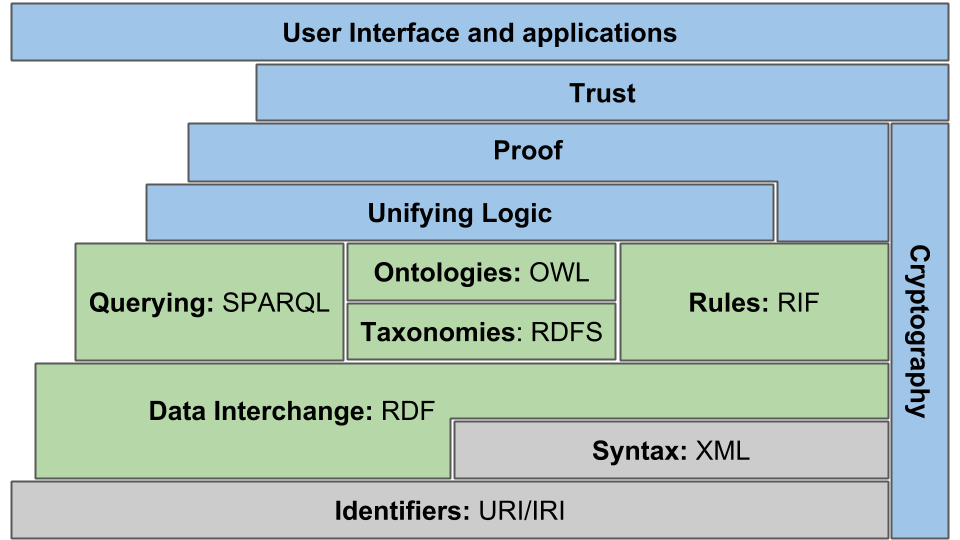
\includegraphics[width=0.8\textwidth]{stack6}
	%\end{adjustwidth}
	\caption[Semantic Web Stack]{Semantic Web Stack.}
	\label{fig:stack}
\end{figure}
%\footnotetext{Source: \url{https://en.wikipedia.org/wiki/Semantic_Web_Stack}}
Each layer placed on top of other layers  depends on  these other layers but not on those above them. Neighbouring layers can, but not necessarily have to make use of each other. 
We go from the bottom of the stack to its top to explain all its elements:

\begin{description}
%  \item[Character Set] To be compatible with the current Web and its applications, but also with textual documents in all languages in general,
%  the Semantic Web relies on Unicode.
 \item[Identifiers] The Semantic Web is a global network which relies on interoperability. In such a big setting, it is crucial that the names of individuals and concepts are unique.
 For their representation Uniform Resource Identifiers (\uris) and Internationalized Resource Identifiers (\iri{}s) are used.  
 \item[Syntax] There are several syntax formats frequently used in the Semantic Web. Standards of the World Wide Web are employed---such as XML or JSON---but also formats 
 only created for the Semantic Web such as for example the Terse RDF Triple Language (Turtle). 
%  The fact that the Semantic Web stack only mentions XML and omits 
%  other notations which are also used
%  is often 
%  a point of criticism.\footnote{See for example the discussion at: \url{https://lists.w3.org/Archives/Public/semantic-web/2016Feb/0121.html}.} 
 \item[Data Interchange]
In order to exchange data it must be agreed on  a common structure to express knowledge. This 
structure should not be too complex for a machine to parse but still 
powerful enough to make simple statements and connections. 
In the Semantic Web the Resource Description Framework (\rdf) was developed with 
that goal in mind. Knowledge is expressed using simple triples consisting of subject,
predicate and object. By using unique names (\iri{}s and \uris) connections between different triples are made. 
Ideally, one resulting graph then forms the Semantic Web.
 \item[Taxonomies] For the simple classification of objects and properties the Semantic Web uses the standard \rdf Schema (\rdf{}S). \rdf{}S extends the basic representation format 
 \rdf by several predicates with a predefined meaning such as for example \texttt{rdfs:subclassOf} to denote that one class is a subclass of another. 
 %
 \item[Ontologies]
 The taxonomy already gives some basic information about concepts and individuals in the web. To express more complex things in a fixed way, ontologies are used. 
 Ontologies can be understood as a collection of statements about concepts, classes and individuals using a broad variety of logical predicates which have a fixed meaning for the computer.
 Even though, in that sense a collection of rules over \rdf data could be understood as an ontology,  in the Semantic Web context the term refers to a set of statements written in the Web 
 Ontology Language (\owl). This language is based on description logics and a reasoner can use these statements to draw conclusions.
 %
 \item[Rules] Alternatively to \owl, but also in combination with this standard, there is another way of stating knowledge about concepts and data in the Semantic Web: rules. 
 Having their origin in classical logic programming, rules are used to directly state which triples or patterns of triples can be concluded from given information. To combine rule-based reasoning 
 with \owl reasoning the Semantic Web Rule Language (swrl) can be used. As a general format to exchange different kinds of rules, the Rule Interchange Format (RIF) was created. 
 There are also many other 
 rule-based logics used in the Semantic Web which are not standardised (yet), one of them is \notationthree Logic (\nthreelogic) 
 which is the subject of this thesis.
 %
 \item[Querying] Independently of whether reasoning is performed on \rdf data or not, there are many situations in which a user or an application wants to retrieve information 
 by searching for triples of a certain kind. Therefore, querying is an important part of the Semantic Web. To query data from \rdf the SPARQL Protocol And RDF Query Language (SPARQL) is used.
 \end{description}
 The different layers described so far have---at least up to some point---already been realised---for all building blocks there exist standards. 
 The higher layers we discuss now
are either not realised yet or the community has not yet agreed on a solution (or even on a concrete definition of the problem). 
% In that sense the  following description might be subjective. For alternative views we recommend for example 
% the introduction done by Hogan \cite{hogan}.
 \begin{description}
 \item[Unifying Logic]
 Above these concepts of querying, ontologies and rule based reasoning, there is the layer of a unifying logic: 
 a logical framework which connects the other concepts and makes it possible interoperate between them. 
The logic should thus support the inference mechanisms of these three underlying concepts and the formats below, in particular \rdf.
 \item[Proof]
 Once this unifying logic is found, it should be possible to provide formal proofs for the derivations done using this logic (and thereby also for all derivations of the underlying standards). 
 These proofs should be exchangeable by different parties and it should be possible to automatically check their correctness. Additional information like for example the source of knowledge 
 used could also form part
 of these proofs.
 \item[Cryptography]
 The cryptography layer lies aside of the layers discussed so far. For all the resources and at all layers of the Semantic Web cryptographic techniques should be used 
 to for example verify the identity of an agent or to implement access control mechanisms. Here, existing Web technologies and protocols like for example RSA or HTTPS but 
 also newer techniques like blockchain could be used.
 \item[Trust]
 The layers proof and cryptography together form the base for the trust layer: only if reasoning steps, sources of information and the trustworthiness of all parties involved
 can be verified and manipulation 
 can be excluded, people and machines can trust the information they get from the Semantic Web.
 \item[User interface and applications]
 This highest layer of the stack is also the broadest: a Semantic Web only makes sense if it is more than a scientific construct. 
 It needs to be used by humans but also by different machines which, following
 the original vision, should be able to interact between each other and make use of the resources available. Of course there are already applications making use of the Semantic Web implemented, but
 together with the progress of the Semantic Web as a whole, we expect a lot more to come.
\end{description}

%After having briefly introduced the Semantic Web Stack, it is worth to mention that there are different points which are 
% Introduction given by Hogan \cite{hogan}.
% Gerber \cite{Gerber} \cite{Gerber2}. Really nice: abstracts from technnologies. Bad: the word ``unifying Logic'' dissapeared.
% 
% Ian Horrocks: two towers \cite{twotowers} -- by supporting the closed world assumption we get two semantic webs.
% 
% 
% \cite{rearch} Paper by Boley, Kifer, etc. ``realistic'' architecture, not just one technology. 
% 
% 
% \subsection{Data Interchange}
% RDF
% 
% \cite{rdf}
% \subsection{Querying}
% \subsection{Ontologies}
% RDFS
% OWL
Introducing the Semantic Web stack, its critical points should also be discussed:

%Above, we explained, that the upper layers of the Semantic Web stack should depend on the lower ones, this particular detail often leads to discussion on several levels  

One problem which often leads to disputes\footnote{See for example: \url{https://lists.w3.org/Archives/Public/semantic-web/2016Feb/0121.html}} 
is that the current stack explicitly names XML~\cite{XML} as a base for the syntax while many applications rather use formats like 
the JSON-based JSON-LD~\cite{jsonld} or Turtle~\cite{turtle}, 
which is also easy to read for humans, to represent \rdf.\footnote{Even though in the case of Turtle this point 
is somehow addressed as the \rdf layer directly 
touches the layer of identifiers which are directly used by Turtle.} This is certainly a valid criticism. 
However, in this thesis we see the formats occurring in the stack as open lists of formalisms which have already been standardized to serve the purpose mentioned 
rather than a simple declaration of the decision in favour of a format. To emphasize this, we added to every layer which is labelled with a standard also the general purpose this layer 
fulfils. These names are not always present in the original stack our figure is based on.

Another detail of the stack which is often criticised has to do with the middle layer: While \owl and SPARQL are concrete logics---in case of \owl 
with sub-logics~\cite{OWLRL}---disposing 
over their own clearly defined unambiguous semantics (see \cite{owlrdfsem,owldsem} 
and \cite{sparql}, respectively), RIF~\cite{rif} is a format to interchange rules. Being designed for that purpose, RIF supports different paradigms with sometimes 
conflicting model-theoretic semantics (eg well-founded vs stable semantics) or even with no model-theoretic semantics at all: 
for the RIF Production Rule Dialect (RIF-PRD)~\cite{rifprd} only operational semantics is defined. 
As a connection between these formats, RIF offers RIF Core \cite{rifcore}, a minimal rule language supporting common features of rule languages which can be 
extended to define the semantics of concrete languages.
This broad support of different forms of rule-based languages makes it easy to create a new rule language and relate it to the standard---in that sense it is really
appealing from a theoretical point of view---but it also forms a burden for the bigger goal
behind the Semantic Web Stack: the realisation of the Semantic Web. Practitioners creating applications want to \emph{use rules}
and not  \emph{create or compare rule languages}. For the outsider the complex RIF landscape can be overwhelming. This is one possible reason why the 
full potential of RIF is barely used in practice. 

% Another aspect weakening the position of RIF in the stack is that its syntax is directly based on XML 
% and not on \rdf which offers different syntactic variants of which only one is \rdf/XML. 
% This makes the connection to \rdf rather loose

As discussed above, the upper layers of the Semantic Web stack should depend on the lower ones. 
Above, we already discussed that in the case of the syntax layer this is not always the case 
since XML is only one syntactical option to represent \rdf. The dependency problem is also given for the upper layers depending on \rdf:

RIF is independent of \rdf and poses own semantic definitions. The integration of \rdf into RIF can be done using so-called slots, an extra note~\cite{rifrdf} 
explains how RIF dialects 
can be semantically aligned with \rdf. 
%\rdf and \owl can be integrated to RIF via so-called slots, the   
%
%Nevertheless, even this group of 
%This means that it is a family of logics which do not all have Semantics defined.
%As it is, RIF is a very good format to \emph{define} languages, but with its oneness   
% Being a very open standard, RIF misses the opportunity to force the community to stick to a certain rule format which is crucial if we have in mind that it was created to 
% serve : the crea Semantic Web.
%RIF is standardised disagreement

SPARQL has its own query semantics which is agnostic about the meaning of \rdf triples. For SPARQL these are only patterns but these patterns need to be aligned 
with the search patterns of SPARQL.

More problematic is the relationship of \owl and \rdf. \owl  has been designed on the base of Description Logics~\cite{dl}. a logical framework based on First Order Logic 
which---in contrast to the latter---has the advantage to be decidable. For \owl there exist two syntaxes, one direct syntax 



In my opinion, only SPARQL is compatible with RDF (but I have to think about it) -> naja, sparql definiert nur query pattern und is in gewissen sinne agnostisch was die bedeutung der triple betrifft.

Here: Problems with Ontology layer

Even the parts realised have certain ``cracks'' or problems. It was mentioned earlier that all higher layers should rely
on the layers beneath them. That said, one would expect that \owl would be compatible with \rdf{}S---and there exists a version which actually is, \owl full. 

Must it even be \emph{one} unifying logic?

\section{The Unifying Logic}



Mention: RDF is only compatible with owl full

\cite{twotowers} think that the rules and owl should not be side by side, they see the open world assumption as problem and want to have the rule layer on top of owl dl.

Maybe also mention that the connection of owl and rdfs is rather artificial -> two semantic definitions...

%\subsection{Rule Based Logics}

History about big discussion open vs. closed world assumption.

Discussion: closed world assumption a problem

comes also in \cite{rearch}.

Solution:scoped negation as failure.

The paper above sees rules without negation as failure such as swrl just as extension of owl and not as belonging to the other format.

rules and owl see each other as black boxes.
we can combine them
-> this reminds me a little bit of validation where we first do dl reasoning and then querying

the paper also see querying as some kind of rule application (I think they are right here).


RIF

SWRL

N3

\cite{N3Logic}

Explain this unifying logic, list the attempts to find one and answer the question: why N3 and not those?



Here or somewhere else mention description logic programs \cite{DLP} which try to combine Description Logic and Logic Programming. - OK, rather their intersection.

\cite{knorr} rules as unifying logic

\cite{unilogic} first attempt to close the rift between rule-based and description logic reasoning, problem remains: open world assumption


What do we expect from the ``unifying logic''?

The vision of the Semantic Web is to enable machines to use the Web just as humans do. For that they need to be able to \emph{understand} and \emph{exchange} data through the Web. 
An unambiguous way to express knowledge is needed, a logic. 
This logic needs to be well defined to avoid misunderstandings and it needs to be agreed on this definition between all possible parties involved.


Different approaches in the ``quest for a unifying logic'': extend owl (nominal schemas, same paper \cite{unilogic}), ``merge'' owl and rules (both mentioned in \cite{unilogic}). We go a third way: rules for all.

approaches consider worst case time complexity (e.g. \cite{unilogic}). -> argue that this is nice but we focus on practical cases.

OWL and rdf is already artificial, rules are natural extension of RDF and the can cover owl.

Later on mention integrity constraints on data bases which are needed for validation.

Artikel von Motnik \cite{DLASP} sagt was ueber default rules for validation -> validation ist ein ziemlich interessantes Thema hier.

unifying logic on application level, not just a construct -> we therefore exclude owl full.

allgemein: answer set programming hat zwei Formen der Nagation.

noch was von Lifschitz und asp zitieren.


Also say why you should go for N3: unifying logic is not just a theoretical construct, it also gives practical advantages: reasoning is often faster when you use only one logic.  

somewhere: reification is not the same as citation.

Knorr hat DL style syntax
It has advantages if you need 
the features of different frameworks. Of course, if you know that, eg only querying is needed you should still go for SPARQL.


% The Unifying Logic needs to be well-defined in itself, it needs to be able to ``understand'' the underlying formats, in particular to query, do DL reasoning and use rules. 
% Additionally it should provide the opportunity to connect to the proof layer.
Requirements:
\begin{description}
 \item[clear semantic definition] 
The meaning of every statement needs to be clearly defined.
 \item[compatibility with existing Web standards]  Existing standards of the Semantic Web need to be supported. 
 In particular, querying, Description Logics, and rule based reasoning need to be covered.
 \item[support of proofs] It must be possible to express, interchange and check all derivations made in the logic.
 \item[capability to handle change] It must be possible to express and reason about change.
\end{description}



\section{Research questions}
Question: Is N3 a suitable candidate to become the unifying logic for the semantic web?

Sub-questions:

Can we give a clear semantic definition of Notation3 Logic?

How does Notation3 Logic interfere with other formats? Can SPARQL, OWL and RIF be expressed?

Is it possible to express proofs in N3?

Can N3 handle change?

I think I need to be more specific. To find that: what do I actually do here?



% \textbf{Part 4: going beyond the limits}
% 
% introduce weighted transition logic to express change
% 
% This part is optional



Somewhere I need to talk about problems, especially decidability and for example the problems of OWL full.

Should I have a chapter about negation as failure?

Problem: blank nodes in SPARQL

%\part{Semantics}

\chapter{Implicit Quantification}\label{problem}\label{semantics}










%When introducing \nthreelogic in Section~\ref{n3examples} we also
% In Section~\ref{n3examples}  we already briefly introduced \nthreelogic by discussing several examples and their intended meaning. We furthermore explained 
% that this \emph{intended meaning} 
% is problematic:
The semantics of \nthreelogic is only defined in an informal way by the \wwwc team submission~\cite{Notation3} and a journal paper~\cite{N3Logic}. 
This leaves room for interpretation and it actually leads to contradicting implementations. 
In this chapter, we take a closer look at this problem and its possible solutions. % and the related \hyperlink{rq2}{Research Question 2}.
%We first briefly discuss the semantics of \rdf, the logic \nthree extends, and have a look at possible challenges
%In order to answer  and test \hyperlink{h2}{Hypothesis 2} we create several test cases .  
We first collect evidence %for this problem 
by giving concrete example formulas which, when given to the reasoners Cwm~\cite{cwm} and EYE~\cite{eye}, lead to different results. 
The discrepancies we encounter are mainly related to 
implicit quantification: \nthree allows the use of quantified variables whose universal or existential quantifier is not explicitly stated but implicitly assumed.
% Having understood this difficulty To understand how such a concept can be formalised, we discuss other frameworks which support implicit quantification and their semantics. Here we especially 
% focus on \rdf, the logic which is extended by \nthree: blank node in \rdf are understood as implicitly existentially quantified.
The problem can be solved by providing a formalisation which clearly indicates how implicit quantification needs to be interpreted. To better understand how such a formalisation 
could look like we discuss different logics supporting some kind of implicit quantification, in particular \rdf and other formats related to the Semantic Web, and discuss
in which aspects they differ 
from \nthree.

% We encounter similar concepts in other logics and especially in 
% %Similar concepts can be found in other logics, in particular in 
% \rdf where blank nodes are understood as implicitly existentially quantified. 
% % To better understand how implicit quantification can be handled in a formal model a closer look to \rdf semantics and the conclude this section
% % by discussing implicit quantification in general.
% In order to find a way to formally describe the semantics of \nthree we take a closer look to \rdf{}'s semantics and implicit quantification 
% 


% To put our observations into context, we then discuss how the concept of implicit quantification is handled in related contexts. In particular we give an overview of 
% \rdf semantics and 
% To formalise the difference in the interpretations of implicit quantification, we define a core logic for \nthree which is very close to the original 
% but only allows explicit quantification. 
% One part of such implicitly quantified variables are also present in the logic \nthree is based on: \rdf understands blank nodes as existentially quantified variables.
% To better understand how the semantics of a language can deal with implicit quantification we next take a look into \rdf semantics
%This chapter is partly based on the following papers: 

%\basedpapers{arndt_ruleml_2015}.
%
\section{Syntax}
Before coming to the main topic of this paper, implicit quantification, we start by defining the general syntax of N3Logic. We exclude built-ins %, as their 
%meaning is mostly defined on the corresponding website, %\footnote{See \url{http://www.w3.org/2000/10/swap/doc/cwmBuiltins}.},  
and explicit quantification (for more information see section \ref{expl}). %\footnote{We explain this choice in section \ref{expl}. }. 
%The latter is, as well as its implicit counterpart, not trivial. We will give a quick explanation of that at the end of this paper.\\
The syntax-definition below is oriented on the context-free grammar as provided at the team submission web page \cite{Notation3}. 
%We limit our developments to the %, at least in our opinion, 
%most important properties of \nthree---quantification, implication and quoting---and skip most inbuilt-predicates of \nthree and \rdf, whose meaning 
%can be found on the corresponding websites. %We start with the vocabulary:


\begin{definition}[Basic N3 vocabulary]\label{voc}
An \emph{N3 alphabet~$A$} consists of the following disjoint classes of symbols:
\begin{itemize}
\item A set $U$ of \uri symbols.
\item A set $V=V_E\mathbin{\dot{\cup}} V_U$  of (quantified) variables, with $V_E$ being the set of existential variables
and $V_U$ the set of universal variables.
\item A set $L$  of literals.
%\item A boolean literal \verb!false!
\item Brackets \verb!{!, \verb!}!, \verb!(!, \verb!)!
\item Logical implication $\verb!=>!$ 
\item Period \verb!.!
\end{itemize}
\end{definition}

%We define the elements of $U$ in the same way as \rdf \cite{rdf}. %in %the corresponding specification~\cite{iri}.
%Like Turtle, \nthree allows to abbreviate URLs as prefixed names~\cite{turtle}.
%Literals are strings beginning and ending with quotation marks `\verb!"!';
%existentials start with `\verb!_:!', universals with `\verb!?!'.\\
%As \nthree does not clearly distinguish between predicates and constants---a single \uri symbol can stand for both at the same time---we have to change the first-order-concept of a 
%term to something similar:

We define the elements of $U$ as in the corresponding specification~\cite{iri}. As for example in Turtle \cite{turtle},
\nthree allows  to abbreviate URLs by using prefixes.
%\nthree allows to abbreviate URLs as prefixed names~\cite{turtle}.
Literals are strings beginning and ending with quotation marks `\verb!"!';
existentials start with `\verb!_:!', universals with `\verb!?!'.
%
Unlike first order logic, \nthree does not distinguish between predicates and constants---%
a single \uri symbol can stand for both at the same time---%
so the first-order-concept of a~\emph{term}
has a~slightly different counterpart in \nthree: an \emph{expression}.
Since the definition of expressions (Definition~\ref{expression})
is closely related to the concept of a~formula (Definition~\ref{formula}),
the two following definitions should be considered together.

%We include the possibility of quoting formulas by introducing \emph{formula expressions}. Additionally to the direct citation of a formula, there are two other 
%kinds of formula-expressions: the empty expression (true) and \verb!false!. As the latter is inherited from \rdf, it can't be understood as a formula itself as the 
%similar expression in first order logic normally is. The declarations as formula expressions enable us to keep that kind of meaning in controlled situations, as will
%be shown in the following chapters.


\begin{definition}[Expressions]\label{expression}
  Let $A$ be an \nthree alphabet.
  The set of \textit{expressions} $E \subset A^{*}$ is
  defined as follows:
  \begin{enumerate}
    \item Each \uri is an expression.
    \item Each variable is an expression.
    \item Each literal is an expression.
    \item \label{list} If $e_1,\ldots,e_n$ are expressions, $\verb!(!e_1 \ldots e_n\verb!)!$ is an expression. 
    %\item \label{false} \verb!false! is an expression.
   % \item $\verb!{ }!$ is an expression.
    \item \label{fe} If $f\in F$ is a formula, then $\verb!{!f\verb!}!$ is an expression. 
  \end{enumerate}
  The expression defined by \ref{list} is called a \textit{list}.
  We call the expressions defined by %\ref{false}--
  \ref{fe}
  \textit{formula expressions} and denote the set of all formula expressions by $\mbox{\textit{FE}}$.
\end{definition}


Note that point \ref{fe} of the definition above makes use of formulas, which are defined as follows:

\begin{definition}[\nthree Formulas]
    \label{formula}
    The set $F$ of \textit{\nthree formulas} over an alphabet $A$ is recursively defined as follows:
    \begin{enumerate}  
      \item \label{1} If $e_1, e_2, e_3$ are expressions, $e_1~ e_2~ e_3$. is a formula, an \textit{atomic} formula.
      \item \label{2} If $t_1, t_2$ are formula expressions, $t_{1} \verb!=>!~t_{2}.$ is a formula, an \textit{implication}.
      \item \label{n} If $f_1$ and $f_2$ are formulas, $f_1 f_2$ is a formula, a \textit{conjunction}.
    \end{enumerate}
\end{definition}

We will refer to a~formula without any variables as a~\textit{ground formula}.
Analogously, we call such kind of expressions \textit{ground expressions}.
We denote the corresponding sets by $F_g$ respectively $E_g$.\\
%Note that 
%Althouh we see this rarely used in practice, t
The definition explicitly allows all expressions in all positions of atomic formulas. 
Literals or even formula expressions can be subjects, objects or predicates.

%Whether a triple with a 
%
%It is rather unlikely th
%It is rather unlikely that any
%Whether an element 
%The meaning of those expressions depends on the respective interpretation.

%We will refer to a~formula without any variables as a~\textit{ground formula}.
%Analogously, we call expressions without any variables \textit{ground expressions}.
%We denote the corresponding sets by $F_g$ respectively $E_g$.
% We are going to define the semantics of a formula. To enable the reader to distinguish between mathematical symbols describing the language and \nthree-constructs (expressions and formulas), 
% we mark the latter by underlinement. 

In the examples in the remainder of this paper, we will use the common \rdf shortcuts:

\begin{remark}[Syntactic variants]\label{rem}
\begin{itemize}
\item A formula consisting of two triple subformulas starting with the same element \verb!<d> <p> <e>. <d> <q> <f>.! can be abbreviated using a semicolon:\newline 
\verb!<d> <p> <e>; <q> <f>.!
\item Two triple formulas sharing the first two elements  \verb!<d> <p> <e>. <d> <p> <f>.! can be abbreviated using a comma: \verb!<d> <p> <e>, <f>.!
%  \item \verb![]! can be used as an expression and is a shortcut for a new existential variable. So \verb![] <p> <d>.! stands for \verb!_:x <p> <d>.!
%  If $[~]$ occurs in a formula $f$ instead of an expression, each instance of $[~]$  can be translated by a new existential variable.
 \item An expression of the form \verb![<p> <o>]! is a shortcut for a new existential variable \verb!_:x!,
   which is subject to the statement \verb!_:x <p> <o>.! %\linebreak
   So \verb! <s> <p> [<q> <o>].! stands for \verb!<s> <p> _:x. _:x <q> <o>.!
 %\item \verb!a! is a~shortcut for \verb!rdf:type!~\cite{RDF}.
 \end{itemize}
\end{remark}



To emphasize the difference between brackets which form part of the \nthree vocabulary, i.e. ``\verb!(!'', ``\verb!)!'', ``\verb!{!'', and ``\verb!}!'', 
and the brackets occurring in mathematical language, we will underline the \nthree brackets in all definitions where both kinds of brackets occur.
 
 \section{Quantification}\label{quantsec}
%The examples of implicit quantification given in Section~\ref{n3examples} were rather  
The example formulas we discussed in Section~\ref{n3examples} were rather simple and understanding their intended meaning was not 
 difficult (maybe with the exception of cited formulas which can lead to discussions \cite{TriGsemantics}). For the only case where 
two different interpretations were plausible -- Formula~\ref{both} which had universals and existentials occurring together --
the \wwwc team submission~\cite{Notation3} contains a clear statement which interpretation needs to be chosen: \\
% This is different when it comes to implicit quantification. Just like \rdf, \nthree allows the 
% The examples of \nthree formulas given so far were rather easy and their interpretation was rather straightforward
% (maybe with the exception of cited formulas which can lead to discussions \cite{TriGsemantics}).
% This is different when it comes to implicit quantification. Just like \rdf, \nthree allows the usage of implicitly existentially quantified variables, called \emph{blank nodes}.
% Blank nodes either start with ``\verb!_:!'' or are expressed using square brackets ``\texttt{[~]}''. 

\MyQuote{ \label{beide} ``If both universal and existential quantification are specified for the same formula, 
then the scope of the universal quantification is outside the scope of the existentials''.}

Unfortunately, not all cases are that clear.
% 
% 
% in Section~\ref{n3examples}, we gave a few examples for \nthree formulas and their intended meanings. Since \nthree aims to extend \rdf, a \wwwc standard with well-defined 
% semantics, the meaning of simple  
%
% In the cases illustrated in Section~\ref{n3examples}, the interpretation of the implicitly quantified formulas was rather easy:
% the variables are existentially and universally quantified at the top of the formula; 
% if they co-occur in the same formula, the universal quantification dominates the existential. 
When implicitly quantified variables occur in deeply nested formulas, 
 their intended meaning is not always obvious and the interpretations of such formulas sometimes differ between reasoning engines. 
%
%In the next subsections we give examples for such ambiguous formulas.
In this section we want to better understand these differences. 
With this goal, we perform several tests on the reasoners Cwm \cite{cwm} and EYE~\cite{eyepaper} and compare their results. 
Cwm and EYE were chosen because they cover most constructs specified in \nthree{}'s \wwwc team submission. 
In contrast to for example FuXi~\cite{fuxi}, they both support rather complex constructs like nested rules. 
% and because they differ in their way to handle 
% implicit universal quantification.
% Further details about how differences can be detected can be found in our previous paper \cite{arndt_ruleml_2015}. % and in \ref{ap1}.



% 
% Before clarifying syntax and semantics of \nthree in a more formal way than presented in Section~\ref{n3examples}, 
% we test how implicit quantification of \nthreelogic is understood in practice. We  take a look to the official sources of \nthree, namely the \wwwc team submission~\cite{Notation3}
% and the journal paper about \nthree~\cite{N3Logic}, and test, how the reasoners Cwm~\cite{cwm} and EYE~\cite{eye} understand them. 
% We choose these two reasoners because of their coverage: while for example FuXi~\cite{fuxi} only supports \nthree datalog -- a subset of \nthree which does not support nested rules --
% the reasoners Cwm and EYE cover a big part of the specifications
% As in \rdf, atomic formulas are triples consisting of subject, predicate and object. They can be intuitively understood as 
% first order formulas of the form \linebreak $\text{predicate}(\text{subject}, \text{object})$. It is also easy to get an idea of the meaning of conjunctions or implications 
% if no variables are involved. Including implicit quantification is more difficult.
% Definition \ref{voc} distinguishes between two kinds of variables: universal and existential variables. 
% As the names indicate, these variables are meant to be implicitly quantified. But how do we have to understand this ``implicit'' quantification?
% Some cases are quite simple. 
% If we have the formulas
% \[
% \verb! _:x :knows :Kurt.! \text{ and } \verb! ?x :knows :Kurt.!
% \]
% It is rather straight forward to understand them as ``someone knows Kurt.'' and ``everyone knows Kurt.'' In first order logic:
% %We can understand that as the fact that Kurt knows someone or something, written in first order logic:
% \[
% \exists x: \text{knows}(x, \text{Kurt}) \text{ and } \forall x: \text{knows}(x, \text{Kurt}).
% \]
%Similarly simple constructions with universals can be understood:
%\[
%\verb! ?x :knows :Kurt.!
%\]
%Means that everyone knows Kurt, in first order:
%\[
%\forall x: \text{knows}(x, \text{Kurt}).
%\]
% But the above grammar also enables us to construct more complicate statements. Does the construct 
% \begin{equation}\label{both} \verb! ?x :loves _:y.!\end{equation} mean 
% ``everybody loves someone'' or ``there is someone
% who is loved by everyone'', in first order formulas: 
% %\[\forall x \exists y : \text{loves}(x,y) \tag{1}\quad \text{ vs. } \exists y \forall x : \text{loves}(x,y)\]
% \stepcounter{equation}
% \begin{equation} % oder auch align
% \forall x \exists y : \text{loves}(x,y)\quad  \text{ vs. }\quad \exists y \forall x : \text{loves}(x,y) \tag{\ref{both}a, b}
% \end{equation}
% 
% 
% In this case we know the answer, the team submission \cite{Notation3} clearly chooses (\ref{both}a): 
% 
% \MyQuote{ \label{beide} ``If both universal and existential quantification are specified for the same formula, 
% then the scope of the universal quantification is outside the scope of the existentials''.}
% %
% And also the reasoners we tested, in particular EYE and cwm, have implemented the first interpretation (\ref{both}a).
% %\\
% 
% Such clarity is lacking when it comes to nested formulas or co-occurring formula expressions which contain variables. 
% We will treat this in the following sections, first for existential variables, then for universals.
%This is the topic of the following sections.

\subsection{Existentials}\label{existentials}
We start our considerations by taking a closer look to implicit existential quantification in nested formulas, 
ie formulas where the blank node occurs within curly brackets \{~\}.  Such constructs are typically used to cite formulas or
to state rules. We take the following example for the latter:
%An example for such a formula is the following:
% 
% To test how both cwm and EYE understand existential quantification, we confronted them with some examples.
% Both reasoners offer the option to output all knowledge they are aware of, this includes all derived formulas and rules as well as the
% input. In most cases, different variables sharing the same name are renamed to be distinguishable. %standardized apart\footnote{Cwm does standardization apart for existentials, 
% %using square brackets ``\texttt{[ ]}'' as introduced in Remark \ref{rem}, EYE employs Prolog's standardization apart.}. %, in EYE this process includes standardization apart\footnote{As EYE is written in Prolog, 
% %Prolog's standardization apart mechanism is used see e.g. CITATION}.   
% Therefore we can use the derived output of such a reasoning process with a simple rule as input as indication of
% how the formula is interpreted. As a first example %for our tests we took 
% we invoked both reasoners with
% a formula with nested existentials:
\begin{equation}\label{eq1}
\verb!_:x :says {_:x :knows :Albert.}.!
 \end{equation}
%  \begin{equation}\label{eqrule}
% \verb!{_:x :knows :Albert.}=>{:Albert :knows _:x.}.!
%  \end{equation}
This triple is interesting because it contains the blank node \texttt{\_:x} at two positions: as a subject of the triple and inside a nested formula. We already know 
that a blank node represents an implicitly existentially quantified variable, but what we do not know yet is: what is the exact position of its quantifier 
and what is the scope of the variable? Depending on the answer, the two occurrences of \texttt{\_:x} could either refer to the same instance of the domain of discourse, 
then the formula means
%The formula could either mean
%
\[\exists x : \text{says}(x, \text{knows}(x, \text{Albert})) \tag{\ref{eq1}a} \label{zwei}\]
\begin{center}\textit{``There exists someone who says about himself that he knows Albert.''}
  \end{center}
  or 
%   it can refer to two (possibly) different individuals. Here, we have two options:
    the \texttt{\_:x} is always quantified in the direct formula it occurs in (ie the brackets \texttt{\{~\}}), then the two existentials can refer to different objects 
  and we get
%  
% \[
% \exists x_1 : \exists x_2: \text{says}(x_1, ( \text{knows}(x_2, \text{Albert})))\tag{\ref{eq1}b} \label{zw1}\]
% \begin{center}\textit{``There exists some $x_1$ and some $x_2$ and  $x_1$ says about $x_2$ that he knows Albert.''}\end{center}
\[
\exists x_1 : \text{says}(x_1, (\exists x_2: \text{knows}(x_2, \text{Albert})))\tag{\ref{eq1}b} \label{zw}\]
\begin{center}\textit{``There exists someone who says that there exists someone (possibly someone else) who knows Albert.''}\end{center}
\begin{lstlisting}[
  float=t,
  caption={Reasoning result of cwm for Formula \ref{eq1}. The two occurrences of the variable \texttt{\_:x} get translated to two blank nodes in square bracket notation. },
  label=cwm1]
§\textcolor{gray}{@prefix : <http://example.org/ex\#>.}§

[ :says { [ :knows :Albert ]. } ].
\end{lstlisting}

\begin{lstlisting}[
  float=t,
  caption={Reasoning result of EYE for Formula \ref{eq1}. The two occurrences of the variable \texttt{\_:x} get translated to two different blank nodes.},
  label=third]
§\textcolor{gray}{PREFIX : <http://example.org/ex\#>}§

_:t_0 :says {_:t_1 :knows :Albert}.
\end{lstlisting}
As explained earlier in Section~\ref{prn3}, \nthree reasoners can be invoked to output the deductive closure of their input files. If we provide 
Cwm and EYE with Formula~\ref{eq1}  and let them derive the deductive closure we get the result displayed in Listings~\ref{cwm1} and \ref{third}, respectively.\footnote{
Unless indicated otherwise we use in this thesis the following versions of the reasoners:
Cwm v 1.197 2007/12/13 15:38:39 syosi and EYE v18.0312.0936}
We see, that Cwm uses the bracket notation \texttt{[~]}  for blank nodes where, as explained in Section~\ref{vars}, every new bracket refers to a fresh new blank node; 
EYE gives them different names (\texttt{\_:t\_1} and \texttt{\_:t\_2}). This behaviour shows, that both reasoners understand the two occurrences of \texttt{\_:x} as different 
blank nodes which results in Interpretation~\ref{zw}.%
\footnote{
Strictly speaking, this example still does not make sure that the reasoners really assume Interpretation~\ref{zw} since both blank nodes could be quantified on top level:
$\exists x_1 : \exists x_2: \text{says}(x_1, ( \text{knows}(x_2, \text{Albert})))$.
To exclude this possibility the reasoners can be tested with Triple~\ref{simple} and the rule \texttt{\{\_:x :knows :Albert.\} => \{:Albert :is :known.\}.}: only if 
the quantifier for the blank node is in the antecedent of the rule, this input results in \texttt{:Albert :is :known.} This is the case for both reasoners.
}
%but we do not know from that example, whether this separation really results in Interpretation~\ref{zw}. It could still be that the reasoners understand the quantifier

% Strictly speaking, this example still does not make sure that the reasoners really assume Interpretation~\ref{zw} since the quantifiers for the blank nodes in the formulas are 
% not written down and the formula could still have the following meaning:
% \[
% \exists x_1 : \exists x_2: \text{says}(x_1, ( \text{knows}(x_2, \text{Albert})))\tag{\ref{eq1}c} \label{zw1}\]
% \begin{center}\textit{``There exists some $x_1$ and some $x_2$ and  $x_1$ says about $x_2$ that he knows Albert.''}\end{center}
% To exclude this possibility, we do one extra test. Depending on the position of the existential quantifier the rule 
% % Is there someone who says about himself that he knows Albert, or does this someone just state that someone exists who knows Albert?
% % In first order logic
% % \[\exists x : \text{says}(x, \text{knows}(x, \text{Albert})) \tag{\ref{eq1}a}\]
% % \hspace{6cm} or
% % \[\exists x_1 : \text{says}(x_1, (\exists x_2: \text{knows}(x_2, \text{Albert})))\tag{\ref{eq1}b} \label{zwei}\]
% % %
% % Listing \ref{third} shows the output of EYE given formula (\ref{eq1}) as only input, Listing \ref{cwm1} the output of cwm. 
% % We clearly see\footnote{To see this evidence 
% % for cwm, recall that every new bracket ``\texttt{[}$\ldots$\texttt{]}'' corresponds with a \emph{new} existential variable, see also Remark \ref{rem} or \cite{turtle} for further information. }
% % that both reasoners favor 
% % option (\ref{zwei}).  
% 
% 
% 
% %\footenotetext
% 
% %\FloatBarrier
% % 
% % 
% % We observe similar behavior using the same existential quantifier in two co-occurring graphs.
% % In an example formula such as 
% %
% \begin{equation} \label{ruru}
% \verb!{_:x :knows :Albert.} => {:Albert :is :known.}.! 
% \end{equation}
% either translates to
% \[
% (\exists x: \text{knows}(x,\text{Albert}))\rightarrow \text{is}(\text{Albert}, \text{known})\tag{\ref{ruru}a}
% \]
% in which case the formula is equivalent to 
% \[
% \forall x:( \text{knows}(x,\text{Albert}))\rightarrow \text{is}(\text{Albert}, \text{known})\tag{\ref{ruru}a'}
% \]
% or it translates to
% \[
% \exists x:( \text{knows}(x,\text{Albert}))\rightarrow \text{is}(\text{Albert}, \text{known})\tag{\ref{ruru}b}
% \]
% These two options can be tested against each other by giving Rule~\ref{ruru} to the reasoners together with Triple~\ref{simple},
% $\verb! :Kurt :knows :Albert.!
% $, if the reasoners derive 
% \begin{equation}
%  \verb!:Albert :is :known.!
% \end{equation}
% we can assume that they favour 
% 
% 
% %So, for EYE, the scope of existential quantification is always only the direct formula expression the existential occurs in but 
% %not it nested dependencies.
% The two \verb!_:x! are interpreted as different variables by both reasoners. In first order logic this would be:
% \[
%  (\exists x_1: \text{knows}(x_1, \text{Albert}))\rightarrow (\exists x_2: \text{knows}(x_2, \text{Kurt}))
% \]
%
%
%
This example shows what is meant by the following quote from the \wwwc team submission \cite{Notation3}:

\MyQuote{
``When formulae are nested, \_: blank nodes syntax \emph{[is]} used 
to only identify blank node in the formula it occurs directly in. 
It is an arbitrary temporary name for a symbol which is existentially quantified within the current 
formula (not the whole file). They can only be used within a single formula, and not within nested formulae.''
}
%
%This means, the scope of an existential quantifier is always only the formula-expression ``\verb!{!$\ldots$\verb!}!'' it occurs in, but not its nested dependency.
%We added these two examples to be able to compare the interpretation of existential quantification with universal quantification.
%Although this section might not seem surprising, we included the above 
%We keep these examples for the scoping of existentials in the paper, to be able to emphasize the different scopes of existential and universal quantification.
In other words: existential variables are always quantified in the direct formula -- marked by curly brackets \texttt{\{~\}} -- they occur in. 
This quantifier does always only count for that formula and not for the nested formulas depending on it.


\subsection{Universals}\label{universals}
The case of implicit existential quantification in \nthree was still clear and the reasoners we tested did not disagree on the meaning of implicitly existentially 
quantified variables. This is different for universal quantification. A typical example for a formula containing universal quantification was given before in Formula~\ref{uni}:
\begin{multline}\tag{\ref{uni}}
 \texttt{\{:Kurt :knows ?x.\} => }%} \\ \texttt{
 \texttt{\{?x :knows :Kurt.\}.}%\nonumber
\end{multline}
It would not be very useful to handle the quantification in this equally as existential quantification. If universal quantifiers where also always quantified on their direct 
formula we would get the interpretation:
\[\tag{\ref{uni}a}
(\forall x_1: \text{knows}(\text{Kurt}, x_1))\rightarrow (\forall x_2: \text{knows}(x_2, \text{Kurt}))
\]
\begin{center}\textit{``If everyone knows Kurt then Kurt knows everyone''}
  \end{center}
Here, we would never be able to write any rules which reason on \rdf triples since this rule only gets invoked for a universal statement -- ``\textit{Everyone knows Kurt.}'' 
--  but it is not possible to 
make universal statements in plain \rdf. Therefore, the interpretation we already discussed earlier in Section~\ref{vars} is correct in this case:
\[\tag{\ref{uni}b}
\forall x:(\text{knows}(\text{Kurt}, x))\rightarrow (\text{knows}(x, \text{Kurt}))
\]
\begin{center}\textit{``Everyone Kurt knows also knows Kurt.''}
  \end{center}
The quantifier for both occurrences of \texttt{?x} is in front of the whole formula. But what happens if the universal variable occurs in a deeper nested formula? 
% We test 
% that on the following example:
% 
% 
%
Here,
the \wwwc team submission states the following:\\

\MyQuote{
 ``There is a also a shorthand syntax ?x which [...] implies that x is universally quantified not in the formula but in its \textbf{parent formula}.''}
We learn that universal variables are quantified on their \emph{parent formula}. Unfortunately neither the \wwwc team submission nor the journal paper about \nthreelogic 
provide us with a definition of that concept. We therefore perform some tests to better understand which formula is the parent.
 
Consider the following formula:
%When it comes to the definition of the scope, universal quantifiers are more complicated. To illustrate that, we consider the following example:
%Another example is the following formula:
%\\ %s and this is also how it is implemented in the reasoners we are considering in this paper, cwm and EYE. 
%It gets even more difficult when it comes to nested rules. As the critical example for this paper, we consider the formula 
\begin{multline}
\texttt{\{\{?x :p :a.\} => \{?x :q :b.\}.\} =>}\\
\texttt{\{\{?x :r :c.\} => \{?x :s :d.\}.\}.} \label{eq2} \end{multline}
Are all \verb!?x! the same? If not, which ones do we have to understand as equal and where are they quantified? 
Of the several options to interpret this formula, two seem to be most likely:
\[\forall x: ((p(x,a)\rightarrow q(x,b))\rightarrow ( r(x,c) \rightarrow s(x,d)))\tag{\ref{eq2}a}\label{ei}\]
\begin{center}or\end{center}
\vspace{-\baselineskip}
\begin{multline}
(\forall x_1: p(x_1,a)\rightarrow q(x_1,b))\rightarrow (\forall x_2: r(x_2,c) \rightarrow s(x_2,d))\tag{\ref{eq2}b}\label{ci}
\end{multline}
%But which interpretation is correct?
% \[
% (\forall x_1: p(x_1,a)\rightarrow q(x_1,b))\rightarrow (\forall x_2: r(x_2,c) \rightarrow s(x_2,d))\tag{\ref{eq2}a}
% \]
% \hspace{6cm}or
% \[\forall x: ((p(x,a)\rightarrow q(x,b))\rightarrow ( r(x,c) \rightarrow s(x,d)))\tag{\ref{eq2}b}\]
%In interpretation \ref{ci}, 
Interpretation~\ref{ei} understands the top formula as the parent of all other formulas, the quantifier for all occurrences of \texttt{?x} is on that formula.
For Interpretation~\ref{ci} the parent of the first two occurrences of \texttt{?x} is the formula 
\begin{equation}
\texttt{\{?x :p :a.\} => \{?x :q :b.\}.}\label{sub1}
\end{equation}
and the parent of the third and fourth occurrence of \texttt{?x} is the formula
\begin{equation}\texttt{\{?x :r :c.\} => \{?x :s :d.\}.}\label{sub2}\end{equation}
Therefore, these formulas carry quantifiers.

If a reasoner follows Interpretation~\ref{ei}, Formula~\ref{eq2} applied on the following rule
\begin{equation}\label{ss1}
 \texttt{\{:e :p :a.\} => \{:e :q :b.\}.}
\end{equation}
results in
\begin{equation}\texttt{\{:e :r :c.\} => \{:e :s :d.\}.}\label{ss2}\end{equation}
While this result cannot be derived by following Interpretation~\ref{ci}. %However, the latter yields Formula~\ref{sub2} when provided with Formula~\ref{sub1}.


If we test the reasoners Cwm and EYE with Formulas~\ref{eq2} and \ref{sub1} as input we get the results displayed in Listing~\ref{cwm2},\footnote{The 
predicate \texttt{log:implies} present in the original output is replaced here by implication arrow \texttt{=>}. The two symbols have the same meaning.} \ref{forth}, respectively.
\begin{lstlisting}[
  float=t,
  caption={Output of cwm for for Formulas~\ref{eq2} and \ref{ss1}. The reasoner does not derive Formula~\ref{ss2}. },
  label=cwm2]  
§\textcolor{gray}{@prefix : <http://example.org/ex\#>.}§
§\textcolor{gray}{   @prefix unive: <\#> .}§
{:e :p :a.}  => {:e :q :b .}.

{@forAll unive:x . {unive:x :p :a .}=>{unive:x :q :b.}.} 
=> 
{@forAll unive:x . {unive:x :r :c .}=>{unive:x :s :d .}.}.
\end{lstlisting}
\begin{lstlisting}[
  float=t,
  caption={Output of EYE for Formulas~\ref{eq2} and \ref{ss1}. The reasoner derives Formula~\ref{ss2}.  },
  label=forth]  
§\textcolor{gray}{PREFIX : <http://example.org/ex\#>}§

{{?U_0 :p :a}=>{?U_0 :q :b}}=>{{?U_0 :r :c}=>{?U_0 :s :d}}.
{:e :p :a} => {:e :q :b}.
{:e :r :c} => {:e :s :d}.
\end{lstlisting}
% The universals in the antecedent and consequent of the main implication reside in two different scopes.
% %This reflects Cwm's interpretation. % as two subformulas:
% Here, it is important that Formula~\ref{eq2} is composed of the subformulas:
% \begin{equation}
% \texttt{\{?x :p :a.\} => \{?x :q :b.\}.}\label{sub1}
% \end{equation}
% \begin{center}  
% and 
% \end{center}
% \begin{equation}\texttt{\{?x :r :c.\} => \{?x :s :d.\}.}\label{sub2}\end{equation} %are direct sub-formulas of formula \ref{eq22}. 
% Syntactically this division is marked by the use of curly brackets \texttt{\{\}}.
% Formula \ref{sub1} has two direct subformulas (again marked by brackets), namely:
% \[\texttt{\{?x :p :a.\}} \text{\hspace{0.5cm} and \hspace{0.5cm}} \texttt{\{?x :q :b.\}}\tag \label{\ref{sub1}a,b}\] 
% while
% \[\texttt{\{?x :r :c.\}} 
% \text{\hspace{0.5cm} and \hspace{0.5cm}} \texttt{\{?x :s :d.\}}
% \tag \label{\ref{sub2}a,b}\]are subformulas of Formula \ref{sub2}. 
%While it is rather easy to understand, how implicitly quantified universals are handled in EYE---they are all universally quantified on top level---it is
%worth to take a closer look into the quantification performed by cwm. 
% Cwm now applies the \wwwc team submission:
% 
% 
% \MyQuote{
%  ``There is a also a shorthand syntax ?x which [...] implies that x is universally quantified not in the formula but in its parent formula.''}
% %
We clearly see that Formula~\ref{ss2} is derived by EYE but not by Cwm. 
We furthermore see that the output of Cwm contains the key word \texttt{@forAll} at in beginning of the antecedent and of the consequent of the main rule in Lines 5 and 7. 
Here, this keyword has the same meaning as the first order symbol $\forall$. Cwm follows Interpretation~\ref{ci}.  We see that 
Cwm and EYE understand the concept of a \emph{parent} differently.
For the remainder of this thesis we write $\textit{parent}_c$ when we refer to the parent formula as implemented in Cwm and $\textit{parent}_e$ 
for the concept of a parent realised in EYE.

The previous example reveals a general problem: 
We needed to explain how the \wwwc team submission is \emph{interpreted} by the reasoners EYE and Cwm.
Of course the term \emph{parent formula} could be understood differently 
and only
specific testing made us come to our conclusion that the above are EYE's and Cwm's interpretations. % of the formula.
Most users are not even aware of the differences in interpretations and the lack of a formalism renders it difficult to discuss or even just express them. %---%
To come to a~clear and unambiguous definition of the logic, 
\nthree needs to be formalised and there needs to be a formalism to express the differences of existing interpretations. 
%This way, user can at least know how the
% The term \emph{parent formula} of a formula $f$ is understood as the next formula $g$ either occurring in curly brackets $\{g\}$ or being the top formula 
% for which $\texttt{\{}f\texttt{\}}$ is a direct component. % of the formula itself or -- in case it is a conjunction -- of one of its conjuncts.
% In our example, Formula~\ref{sub1} is the parent formula of Formulas~\ref{sub1}a and b, and Formula~\ref{sub2} is the parent formula of Formulas~\ref{sub2}a and b.
% This explains the scoping in interpretation \ref{ci}. We refer to this understanding of the concept  parent by using the subscript c, we write $\textit{parent}_c$.
% 
% This is the interpretation EYE applies. For the remainder of this paper we refer to this concept of the term by adding the subscript e, ie $\textit{parent}_e$ 
% refers 
% to the parent formula understood as the top formula.
% 
% 
% 
% 
% As above, we gave formula (\ref{eq2}) as input for both reasoners, cwm and EYE. 
% 
% Lines 1-9 of Listing \ref{forth} show the result of EYE which seems to imply\footnote{Where applicable, 
% EYE employs the ``standardization apart'' mechanism of its programming language Prolog.} that EYE supports the second interpretation (\ref{eq2}b), 
% but as it does not differ from the input, 
% we ran another test to verify that and added the formula 
% \begin{equation}\label{eq4} \verb!{:e :p :a.} => {:e :q :b.}.! \end{equation}
% to the reasoning input in order to see whether the reasoner outputs %(\ref{eq2}b) the reasoner's the result should contain the derived formula  
% \begin{equation}\verb!{:e :r :c.} => {:e :s :d.}.!\end{equation}
% as it would be the case with interpretation (\ref{eq2}b) but not with interpretation (\ref{eq2}a). % this formula cannot be derived. 
% The reasoning output of EYE shown in Listing \ref{forth} (all lines)
% verifies
% that EYE interprets all variables with the same name which occur in one single implication equally regardless of how deeply nested they occur. %variables with the same name in all nested formulas  equally within one single implication.
% 
% In contrast to this, Listing \ref{cwm2} shows the result cwm gives.  Here, the keyword\linebreak %\footnote{ For further explanation of the 
% %keyword \texttt{@forAll} see section \ref{expl}.} 
% ``\verb!@forAll!''
% can be understood as its first order counterpart ``$\forall$'' (see Section \ref{expl}). %Here we see a clear difference between that cwm's interpretation of the input differs from EYE. 
% Cwm understands 
% formula (\ref{eq2}) as stated in interpretation (\ref{eq2}a). Here we see a clear difference between the two reasoners.
% 
% 
% %\FloatBarrier
% 
% 
% After examining universals in co-ordinated expressions such as in the above implication, 
% we are also interested in how those variables are handled in subordinated formula expressions, similar to those in formula (\ref{eq1}). 
% We consider the following formula: 
% \begin{equation}\label{nest}
%  \verb!{?x :p :o.} => {?x :pp {?x :ppp :ooo.}.}.!
% \end{equation}
% To learn how the reasoners interpret this formula, we give the simple formula \begin{equation}\label{spo}\verb!:s :p :o.! \end{equation} as additional input. 
% Listings \ref{eye4} and \ref{cwm4} show the reasoning results of EYE respectively cwm. We clearly see that the two reasoners agree in their interpretation 
% and that this interpretation of formula (\ref{nest}) differs from the interpretation of the existential counterpart formula (\ref{eq1}). 
% 
% 
% 
% 
% 
% %Thus, our formalization has to carefully distinguish the interpretation of nested universals and existentials 
% %This particular difference
% %This difference has to be respected in the formalization in section \ref{formal}.\\
% Having considered the contrary behavior of the reasoners in the interpretation of formula (\ref{eq2}), the obvious question is: 
% how is this interpretation meant to be according to the official sources? The team submission \cite{Notation3} states the following:
% %
% %To be sure that this
% %result has the expected meaning, we did two additional tests. For the first one we added the formula
% %\begin{equation}\label{eq3}
% % \verb!{:c :p :o} => {:c :p :o}.!
% %\end{equation}
% %for the second the formula
% %\begin{equation}
% % \verb!{?x :p :o} => {?x :p :o}.!
% %\end{equation}
% %Listing \ref{forth} shows the result.
% 
% 
% 
% 
% 
% 
% 
% 
% 
% %\begin{lstlisting}[
% %  float=t,
% %  caption={Example of nested implications containing a universal variable \emph{(example2.n3)}},
% %  label=first]
% 
% %§\textcolor{gray}{@prefix : <http://example.org/test\#>.}§
% 
% %{
% %  {?x :p :o.} => {?x :p :o.}.
% %} 
% %=> 
% %{
% %  {?x :pp :oo.} => {?x :pp :oo.}.
% %}.
% %\end{lstlisting}
% 
% 
% 
% 
% 
% 
% 
% \begin{lstlisting}[
%   float=t,
%   caption={Output of EYE for formulas (\ref{nest}) and (\ref{spo}) },
%   label=eye4]  
% §\textcolor{gray}{@prefix : <http://example.org/test\#>.}§
% 
% :s :p :o.
% :s :pp {:s :ppp :ooo}.
% {?U0 :p :o} => {?U0 :pp {?U0 :ppp :ooo}}.
% 
% \end{lstlisting}
% 
% \begin{lstlisting}[
%   float=t,
%   caption={Output of cwm for formulas (\ref{nest}) and (\ref{spo}) },
%   label=cwm4]  
% §\textcolor{gray}{@prefix : <http://example.org/test\#>.}§
% §\textcolor{gray}{   @prefix ex: <\#> .}§
% 
% @forAll ex:x .   
% :s :p :o;
%    :pp {:s :ppp :ooo .}.
% { ex:x :p :o .} => {ex:x :pp {ex:x :ppp :ooo.}.}.
% \end{lstlisting}
% 
% 
% 
% 
%  %
% This quote strengthens the position of cwm but also makes the formalization and implementation of Notation3 challenging, 
% %The scope of a variable is its parent formula, but 
% especially considering it together with our observation on equations (\ref{nest}) and (\ref{spo}): %, this gets more complicated, 
% %as the scoping also includes nested formulas.
% %What if this parent formula
% %depends of another formula containing the same variable?
% If a universal variable occurs in a deeply
% nested formula, the scope of this particular variable can either be its direct parent, the parent of any predecessor containing a variable with the same name
% or even the direct parent of a predecessor's sibling containing the same variable on highest level. %Take for example the formula
% Consider for example the formula
% %\small
% \begin{multline}\label{twovars}
%  \texttt{\{?x :p :o.\}=> \{%} \\ \texttt{
%  \{\{?x :p2 ?y.\} => \{?x :p3 ?y.\}.\}}\\ \texttt{=>\{\{?x :p4 ?y.\} => \{?x :p5 ?y.\}.\}.\}.}
% \end{multline}
% %\normalsize
% Which, according to (III), has to be interpreted as the first order formula 
% \[\forall x: p(x,o)\rightarrow ((\forall y_1: p_2(x, y_1) \rightarrow p_3(x, y_1))\rightarrow(\forall y_2: p_4(x, y_2)\rightarrow p_5(x, y_2))) \]
% Note that in this example, there are two different scopes for \verb!?y!, but only one for \verb!?x!. One can easily think of more  complicated cases. 
% %From here on we invite the interested reader to invent more complicate examples and to test them in both reasoners.
% %There is another aspect which is interesting 
% %in this context. It is not mentioned how nested formulas are expected to  be treated.
% %If universal quantification really behaved as existential quantification with the one and only exception that 
% %the quantifier is on the parent level of the formula, the behavior of the reasoners with respect to formula (\ref{nest}) should be similar to 
% %their handling of formula (\ref{eq1}). 
% %As both reasoners agree in their interpretation of the formulas, we understand this rather as a vagueness 
% %in the formulation and see once again the need to formalize Notation3 logic.
% 
% %\clearpage
% 
% %\FloatBarrier 
% 

\subsection{Explicit Quantification}\label{remarkExplicitQuantification}
We already saw above that apart from implicit quantification, \nthreelogic also provides the possibility to explicitly quantify over variables.
To do so, the quantifiers \verb!@forSome!
and \verb!@forAll! are used. With explicit quantification, Interpretation \ref{both}a of Formula \ref{both} can be expressed as follows:
\begin{multline}\notag
 \texttt{@forAll :y. @forSome :x.}\\\texttt{:x :thinks \{:y :is :pretty\}.}
\end{multline}
Seeing this example, the reader might think that the misunderstandings described above could be avoided by only using explicit quantification and that this notation could 
even be used to explain the differences. Unfortunately, that is not the case. Independently of the order they appear in the formula, universal quantifiers are always understood to
be outside of  existential quantifiers in \nthree~\cite{Notation3}.
The formula
\begin{multline}\notag
 \texttt{@forSome :x. @forAll :y. }\\\texttt{:x :thinks \{:y :is :pretty\}.}
\end{multline}
has the exact same meaning as the previous one, namely Interpretation \ref{both}a.\footnote{We suppose that this has historic reasons: 
When \nthree was created, everything, including quantifiers,  was represented in triples. The order of triples should not matter in any context.}
To express Interpretation \ref{both}b, a more complicated 
construction is needed, which could then again lead to different interpretations. 

The peculiarity described above leads to open questions. %is also one of the reasons we exclude explicit quantification from the considerations in this paper. 
For example, what does the following valid \nthree formula mean?
\begin{multline}
 \texttt{@forSome :x. :x :knows \underline{:y}.}\\ \texttt{@forAll :y. :y :knows :x.}
\end{multline}
The scope of the \texttt{@forAll} is outside of the scope of the \texttt{@forSome}, but what about the first occurrence of \texttt{:y} (underlined in the example)? Is \texttt{:y} a universally 
quantified variable or a constant?
This formula is not supported by Cwm and its intended meaning is not specified in any source we are aware of. 
This and many similar examples make explicit quantification in \nthree a complex topic on its own, which is outside 
the scope of this dissertation. Here we focus on implicit quantification.
\section{Blank nodes in RDF}
% Having seen the uncertainties regarding implicit quantification in the last section  we want to take one more step before approaching the main topic of this chapter which is providing a 
% formal definition of \nthree's semantic
%The goal of this chapter is to formalise the semantics for \nthreelogic. Before we provide a logic  
The previous section showed that the meaning of implicit quantification in \nthree is not always obvious. The problems we encountered arise from the fact 
that is is not easy to informally express where exactly universals and existentials are quantified. We therefore want to provide a formalisation.
To better understand how the specific details of \nthree and in particular implicit quantification 
can be formalised, we take a closer look at the logic it is extending: \rdf.
% \rdf does not support implicit univeral quantification -- this concept is only present in \nthree -- but it understands blanknodes just the same way \nthree does: as implicitely 
% existentially quantified variables.
%
% 
% To better understand how implicit quantification can be covered in formal semantics we further explore 
% % When we define a formal model for 
% % \nthreelogic we need to define the meaning of this concept carefully. 
% % Before we discuss how the uncertainties regarding implicit quantification as exemplified in the previous section can be addressed, we take one step back and have a closer 
% % look on how the concept of 
% % implicit quantification is handled in 
%  the logic \nthree is extending, \rdf.
Here, we do not find implicit universal quantification -- this is a concept that \nthreelogic adds to the \rdf 
model -- but implicit existential quantification 
is also present: as in \nthree blank nodes are understood as implicitly existentially quantified variables.
% %
% %\rdf does not support implicit universal quantification but \nthree's concept of blank nodes to specify implicitly existentially quantified variables is inherited from \rdf.
% %  We therefore  
% %  take a closer look to that concept.
% % Since \nthreelogic is based on \rdf and extends this logic, it makes sense to take a closer look 
% % on how the model theory of \rdf is defined and in particular on how implicit quantification is formalised here. \rdf does not support 
% % implicit universal quantification but the concept of blank nodes which indicate implicit existential quantification is also present here and we discuss that below after introducing
% % the more general concepts. %All
% %Before specifying a model theory for N3 we want to use this section to take a closer look to the logic it is most closely related to, \rdf. We briefly summarise here, how \rdf semantics is defined. 
% We discuss which of the ideas and concepts we encounter in the formalisation of \rdf can also be used to define the semantics of \nthreelogic.

\subsection{RDF semantics}\label{rdfsemantics}
We start by discussing \rdf's formal semantics. 
All definitions we display here are taken from the W3C recommendation~\cite{RDFSemantics}.


% \begin{figure}
% \centering\small
% \begin{tabular}{llr}
%   \hline
% %Syntax: &&\\
% %&&\\
%   \texttt{s ::=} && start: \\
% & \texttt{f}& formula\\
% \texttt{f ::= } & & formulas:                 \\  
%     &  \texttt{s p o.}&                atomic formula\\
%     &  \texttt{f f} &                 conjunction\\
% %&&\\
%  \texttt{s ::=}&&terms:                   \\
%             & \texttt{ex} &                existential variable\\
%       & \texttt{u} &                iri\\
%  \texttt{p ::=}&&terms:                   \\
%       & \texttt{u}\hspace{0.3\textwidth} &                iri\\
%  \texttt{o ::=}&&terms:                   \\
%             & \texttt{ex} &                existential variable\\
%       & \texttt{u} &                iri\\
%       & \texttt{l} &                literals\\
% %      &&\\
%   \hline
% \end{tabular}
% \caption{Overview RDF Syntax \label{RDFSyntax}}
% \end{figure}

As mentioned earlier, \rdf and \nthree (see Section~\ref{n3logic}) distinguish between three kinds of symbols:
% Internationalized Resource Identifiers (\iri{}s), literals, and blank nodes.
% In practice, \iri{}s are Unicode strings that conform to the syntax defined in RFC 3987~\cite{iri}, literals 

\begin{definition}[RDF alphabet]\label{rdfsymbs}
The alphabet of \rdf consists of the following disjoint sets of symbols:
the set $\mathrm{IRI}$ of \iri symbols, the set $\mathrm{L}$ of literals and the set $\mathrm{B}$ of blank node symbols. 
\end{definition}

\iri{}s are all Unicode strings that conform to the syntax defined in RFC 3987~\cite{iri}. 
Literals express concrete values such as numbers, strings or dates and consist of a lexical form combined with a datatype \iri and -- depending on the concrete datatype -- possibly 
an additional
language 
tag.\footnote{Our examples often contain literals without a specific datatype. In these cases the datatype  \url{http://www.w3.org/2001/XMLSchema\#string} is assumed.
\texttt{"example"} stands for \texttt{"example"\textasciicircum\textasciicircum<http://www.w3.org/2001/XMLSchema\#string>}.}
The only syntactic condition the \rdf specification puts on blank nodes is that they need to be disjoint from \iri{}s and literals.
In this thesis we follow the turtle syntax~\cite{turtle} which means that we
either  express blank nodes using square brackets ``\texttt{[~]}'' or strings starting with underscore and column ``\texttt{\_:}''.
These symbols can now be combined into triples and graphs:

\begin{definition}[Triples and graphs]\label{rdftrips}
 For the \rdf alphabet consisting of \iri symbols $\mathrm{IRI}$, literals $L$ and blank nodes $B$ we define:
\begin{itemize}
\item An \emph{\rdf triple} \texttt{s p o.} consists of three components: the \emph{subject}  $\texttt{s}\in \mathrm{IRI}\cup\mathrm{B}$, 
   the \emph{predicate} $\texttt{p}\in\mathrm{IRI}$, and
   the \emph{object} $\texttt{o}\in\mathrm{IRI}\cup\mathrm{B}\cup\mathrm{L}$. We denote the set of all \rdf triples by $\mathcal{T}$.
\item An \emph{\rdf graph} is a set of \rdf triples.   We denote the set of all \rdf graphs by $\mathcal{G}=2^\mathcal{T}$.
\end{itemize}
\end{definition}
% In contrast to \nthree where all kinds of symbols can occur in all positions of a triple, \rdf imposes restrictions on the kinds of symbols which can be used as subject or predicate: 
% predicates need to be \iri{}s -- it is not possible to have quantified variables in that position -- subjects can be \iri{}s or blank nodes. 
% Literals are only allowed in object position. 

For the reader familiar with first order logic there is one detail of \rdf{} syntax -- and thereby also of \nthree{} -- which is very interesting: \rdf does not strictly distinguish between 
constants and predicates. The definition allows all \iri{}s in all positions. It is possible to state for example
\begin{equation}\label{urisubpred}
\texttt{ :Kurt :knows :Albert. :knows a :Predicate. }
\end{equation}
This also influences how the interpretation of \rdf triples and graphs is defined:
%the notion of a \emph{simple interpretation} in \rdf:


%For \rdf graphs we now define the notion of a \emph{simple interpretation}:
% \begin{definition}[Triples and graphs]
% Let  $\mathrm{A}=(\mathrm{IRI},\mathrm{L},\mathrm{B})$ be an \rdf alphabet.
% \begin{itemize}
%  \item An \rdf triple $\texttt{s p o.}$ consists of $\texttt{s}\in \mathrm{IRI}\cup\mathrm{B}$, $\texttt{p}\in\mathrm{IRI}$ and $\texttt{o}\in\mathrm{IRI}\cup\mathrm{B}\cup\mathrm{L}$ 
% \end{itemize} 
%\end{definition}




\begin{definition}[Simple interpretation]\label{si}
A \emph{simple interpretation} $\mathrm{I}$ is a structure consisting of the following elements:
\begin{enumerate}
 \item A non-empty set $\mathrm{IR}$ of resources, called the domain or universe of $\mathrm{I}$.
 \item A set $\mathrm{IP}$, called the set of properties of $\mathrm{I}$.
 \item A mapping $\mathrm{IEXT}: \mathrm{IP} \rightarrow 2^{\mathrm{IR}\times \mathrm{IR}}$
 \item A mapping $\mathrm{IS}:\mathrm{IRI}\rightarrow \mathrm{IR}\cup \mathrm{IP}$
 \item A partial mapping $\mathrm{IL}:\mathrm{L} \nrightarrow \mathrm{IR}$
\end{enumerate}
\end{definition}
Next to the domain of discourse (the set of resources $\mathrm{IR}$) as we know it from first order logic,  we additionally have 
a set of properties $\mathrm{IP}$.
The interpretation function $\mathrm{IS}$ maps \iri{}s to the union of $\mathrm{IR}$ and $\mathrm{IP}$. 
\iri{}s can stand for properties, resources or -- as it is the case in Formula~\ref{urisubpred} -- both. 
%Whether something needs to be a property, 
% The sets $\mathrm{IR}$ and $\mathrm{IP}$ do not need to be disjoint.
For properties there is an additional function to determine their meaning, the \emph{extension} $\mathrm{IEXT}$. 
This function  maps  each property to the set of pairs of resources (which can again also be properties at the same time) for which the property holds.
% for which $p$ holds to it. If our Formula~\ref{urisubpred} from above is for example valid under 
% an interpretation $I$ then we have 
% 
% -- which can as in our example Formula~\ref{urisubpred} also be 
% properties. 
% The values of this function are sets of pairs of elements of the domain .
% 
% to the powerset of all pairs
% of elements of the domain $\mathrm{IR}$. This function is used to determine the meaning of a property by assigning it to the set of all pairs of resources which fulfil it. 
% These resources can at the same time properties. 
For ground graphs, \ie graphs which do not contain blank nodes, we get the following definition:
\begin{definition}[Semantic conditions for ground graphs]
A simple interpretation $I$ can be applied to an element $E\in \mathrm{IRI}\cup\mathrm{L}\cup\mathcal{T}\cup\mathcal{G}$ as follows: 
\begin{enumerate}
 \item If $E$ is a literal then $\mathrm{I}(E)=\mathrm{IL}(E)$
 \item If $E$ is a IRI then $\mathrm{I}(E)=\mathrm{IS}(E)$
 \item If $E$ is a ground triple \texttt{s p o.} then $ \mathrm{I}(E)=\text{true}$ if $(\mathrm{I}(\texttt{s}), \mathrm{I}(\texttt{o}))\in \mathrm{IEXT}(\mathrm{I}(\texttt{p}))$, otherwise 
 $\mathrm{I}(E)=\text{false}$
 \item If $E$ is a ground graph then $\mathrm{I}(E)=\text{false}$ if there exists a triple $E'$ in $E$ for which $\mathrm{I}(E')=\text{false}$, otherwise $\mathrm{I}(E)=\text{true}$ 
 \end{enumerate}
\end{definition}
Note, that the mapping $\mathrm{IL}$ from Definition~\ref{si} is only a partial function, \ie it is not defined for all literal values which are syntactically possible. 
The reason for that is that \rdf also covers the semantics of datatypes\footnote{We do not cover datatype semantics here since it is not relevant for this thesis. We refer the reader interested in that topic 
to \url{https://www.w3.org/TR/rdf11-mt/\#literals-and-datatypes}.} and according to that it is possible that a literal does have a referent. 
Triples whose objects are not in the domain of the function $\mathrm{IL}$ are according to point 3 in the above interpretation false.

Having a notation for the meaning of ground terms we now take a closer look at blank nodes: %how implicit existential quantification in \rdf is handled:
\begin{definition}[Semantic condition for blank nodes]\label{rdfbl}
 If $E\in \mathcal{G}$ is an \rdf graph then  $\mathrm{I}(E)=\text{true}$ if $[\mathrm{I}+\mathrm{A}](E)=\text{true}$ for some mapping $\mathrm{A}: \mathrm{B} \rightarrow \mathrm{IR}$, 
 otherwise $\mathrm{I}(E)=\text{false}$.
\end{definition}
\rdf treats blank nodes as implicitly existentially quantified variables. 
A graph is true under an interpretation if there exists one single mapping which assigns resources to all blank nodes occurring in it such that the interpretation of 
the ground graph is true. If we had to make the implicit quantification in \rdf{} -- or at least of the part which is covered by \rdf semantics -- explicit, we would need to 
always put the quantifier on the top formula. In that sense \rdf is simpler than \nthree: \rdf semantics does not cover such nested constructs as we explained earlier when 
discussing Formula~\ref{eq1}.

% Here, we can use such simple single mapping because \rdf{} -- or at least the part of \rdf which is covered by \rdf semantics -- does 
% not support nested structures.


We finish the subsection by defining the concepts of satisfaction and simple entailment:
\begin{definition}[Satisfaction and simple entailment]
Let $E,F,G\in \mathcal{G}$ be \rdf graphs
\begin{itemize}
\item An interpretation  $\mathrm{I}$ \emph{(simply) satisfies} E, written as $\mathrm{I}\models E$, if $\mathrm{I}(E)=\text{true}$.
\item We call E (simply) satisfiable if there exists a simple interpretation $\mathrm{I}$ such that $\mathrm{I}\models E$, otherwise we call it \emph{(simply) unsatisfiable}.
\item $G$ simply entails $E$, written as $G\models E$, if for every interpretation $I$ which satisfies $G$ ($I\models G$), also satisfies $E$ ($I\models E$). 
\item If $E\models F$ and $F\models E$ we call $F$ and $G$ \emph{equivalent}.
\end{itemize}
\end{definition}
% 
% We now come back to implicit existential quantification: \rdf -- or at least in the part of \rdf which is covered by \rdf semantics -- does not support nested constructs. Therefore
% 
% \begin{equation}
% \verb!:Kurt :denies {_:x rdf:type :Unicorn}. !
% \end{equation}
% 
% 
% 
% We now come back to existential quantification in \rdf: 
% Since \rdf{} -- or at least the part of \rdf which is covered in \rdf semantics -- does not allow for nested structures, blank nodes are simply quantified on top level.
% 
% The case of \nthree is more complicated here.
% To understand that we come back to example Formula~\ref{eq1}:
% \[\tag{\ref{eq1}}
% \verb!_:x :says {_:x :knows :Albert.}.!
%  \]
% As discussed above, we need to understand the two occurrences of \texttt{\_:x} as two different blank nodes. If we assume, that the interpretation function for ground graphs 
% can be extended in 
% a way that is also covers cited graphs and that we can find an interpretation that satisfies the formula 
% \[
% \verb!:John :says {:Kurt :knows :Albert.}.!
%  \]
% it is still not enough to 
% 
% \[
% \exists x_1 : \text{says}(x_1, (\exists x_2: \text{knows}(x_2, \text{Albert})))\tag{\ref{eq1}b} \label{zw}\]
% \begin{center}\textit{``There exists someone who says that there exists someone (possibly someone else) who knows Albert.''}\end{center}
%  
The semantics of  \rdf covers two other kinds of interpretations: D-interpretations which handle literals and their datatypes and \rdf interpretations 
which add a few properties and resources with a predefined meaning to the logic. These concepts are captured by the \rdf vocabulary and contain among others the predicate 
\texttt{rdf:type}\footnote{Here and later on in this thesis the prefix \texttt{rdf:} stands for  \url{http://www.w3.org/1999/02/22-rdf-syntax-ns\#}. } which we used above and 
\texttt{rdf:Property}, the class of all properties. 
% The semantic definitions for some elements of the vocabulary are very strict, \texttt{rdf:type} is thoroughly defined, for some others the specification only includes 
% the intended use.   
% 
% The latter define the semantics
% of the \rdf vocabulary which contains concepts like the  predicate \texttt{rdf:type} from above and \texttt{rdf:Property}, the class of all properties. 
The definitions done in this context can directly be added to a 
possible definition of the semantics of \nthree, entailments defined in this context can be covered by adding rules for that. 
%
We therefore omit the discussion of D-interpretations and \rdf interpretations in this thesis.

\subsection{Structural blank nodes}\label{strucblanks}
Next to the definition of \rdf's semantics covered by the concept of simple, D-, and \rdf interpretations, 
the \rdf specification also includes an informal part explaining the intended use of several elements of the \rdf vocabulary. 
Especially %together with 
the concepts explained in this informal part often require constructs using blank nodes which are not really 
meant to express the existence of a resource in the domain of discourse but 
serve a technical purpose: All knowledge in \rdf needs to be expressed in triples. In some cases these triples are rather artificial and 
need to make use of auxiliary blank nodes. In this thesis we call these blank nodes \emph{structural blank nodes}. 
We further explain how such blank nodes are used on the example of \emph{\rdf collections}. 
%which are used to describe list structures in \rdf.

% 
% Many of the concepts which can be represented employing this vocabulary contain blank nodes which -- as discussed above -- need to be understood
% as implicitly existentially quantified variables.
% 
% We do not discuss  all of them here, but we want to take a closer look to the concept of \emph{\rdf collections}. 
Collections are used to describe list structures in \rdf.
\rdf follows a similar idea as for example Prolog~\cite{Prolog,nilsson} or LISP~\cite{lisp}, which both represent lists using a binary 
function. %\footnote{Note that both standards do not strictly distinguish between relations and functions. We chose to use the term ``relation'' in this context.}
Starting with the empty list, the binary function can be used to recursively construct new lists from existing lists by simply adding new elements at their beginning.
To illustrate the idea let us assume that \texttt{f} is the binary function we use in this context and \texttt{nil} is the empty list. If we want to represent a list consisting of 
\emph{Kurt}, \emph{Albert} and \emph{John} we write:
\begin{equation}\label{flist}
 \texttt{f}(\textit{Kurt}, \texttt{f}(\textit{Albert}, \texttt{f}(\textit{John}, \texttt{nil})))
\end{equation}
As \rdf does not allow the use of compound terms in subject or object position of a triple -- we can only use simple \iri{}s, literals or blank nodes -- the above notation cannot be directly
translated to \rdf. % but requires the usage of additional blank nodes.

To express lists \rdf provides the terms \texttt{rdf:first}, \texttt{rdf:rest} and \texttt{rdf:nil}. 
The term \texttt{rdf:nil} corresponds to the term \texttt{nil} from the example above and represents the empty list. The first and the second argument from the above function 
\texttt{f} are expressed by the predicates \texttt{rdf:first} and \texttt{rdf:rest}, respectively. In order to connect these two arguments, blank nodes are used. The list 
from Formula~\ref{flist} can be represented in \rdf as follows:
% 
% 
% , \rdf represents lists by using first-rest pairs: 
% The term \texttt{rdf:nil} stands for the empty list which has no elements.  To extend any existing list, we can use the predicates \texttt{rdf:first}
% in combination with the list-element we want to add
% and \texttt{rdf:rest} together with the existing list. A list consisting of \texttt{:Kurt}, \texttt{:Albert} and \texttt{:John} then looks as follows:
\begin{equation}\label{firstrest}
\begin{split}
&\texttt{\_:c1 rdf:first :Kurt.}\\
&\texttt{\_:c1 rdf:rest \_:c2.}\\
&\texttt{\_:c2 rdf:first :Albert.}\\
&\texttt{\_:c2 rdf:rest \_:c3.}\\
&\texttt{\_:c3 rdf:first :John.}\\
&\texttt{\_:c3 rdf:rest rdf:nil.}  
\end{split}
\end{equation}
Strictly following the definitions in the previous section the above expression means that \emph{there exist} the lists \texttt{c1}, \texttt{c2} and \texttt{c3} 
and that the first element of list \texttt{c1} is \texttt{:Kurt} and the 
rest of the list is \texttt{c2}, that the list \texttt{c2} has \texttt{:Albert} as first element and list \texttt{c3} as rest and that \texttt{c3} has \texttt{:John} 
as first element and the empty list as 
rest. Using \texttt{\_:c1} in a triple is therefore not the same as directly using a list as for example in the formats mentioned above.
%This is not exactly the same as simply naming the list. % and it is for example not clear whether 

% These can be used to construct   
% This principle is not new and also for example also present in Prolog~\cite[p.119 ff]{nilsson}
For lists as the one above, \rdf provides an extra notation. The collection given in Formula~\ref{firstrest} can also be expressed by simply listing its elements in brackets ``\texttt{( )}'':
\begin{equation}
\texttt{(:Kurt :Albert :John) } 
\end{equation}
This notation is syntactic sugar for the above and even when brackets are used instead of first-rest-ladders in \rdf we still have implicit blank nodes and thereby there is also implicit 
existential quantification present.

\subsection{Referencing formulas in RDF}
In Section~\ref{rdfsemantics} above  we learned that \rdf semantics understands blank nodes as implicitly existentially quantified on top level, \ie if a blank node is occurring in a graph 
its existential quantifier is always assumed to be in front of this graph. In this context we also mentioned that this interpretation makes sense 
because the part of \rdf which is covered
by \rdf semantics does not support the concept of referring to other graphs or formulas. Therefore, constructs as we have seen in Example~\ref{eq1} where we had a blank nodes nested in a
cited formula cannot occur here. 

Next to the  part of \rdf which is covered by \rdf semantics there are concepts in \rdf which are syntactically valid but whose meaning is only informally defined. Some of these 
concepts were created to serve a similar purpose as the citation of graphs in \nthree does: in some way they enable the user to reference triples or graphs. 
For our considerations, it is interesting how exactly blank nodes occurring in these referenced graphs or triples are quantified:
Are they quantified on top level or on a lower level? 

Before we further discuss the concepts for referencing formulas and answer the question above for each of it, 
we discuss an example in \nthree to clarify that the exact position of the existential quantifier matters.
Consider the following formula:
%This is what we discuss below.
% Below, we discuss these formats and take a closer look to the exact position of the quantifier 
% We discuss these 
% % formats here and put a special focus on the quantification of blank nodes occurring in the referenced formulas. 
% 
% 
% % can be done
% In \nthree, the situation is more complicated:
% As discussed in the previous section, 
% a blank node occurring directly in an \nthree formula and a blank node occurring in a nested subformula which share the same name
% %a blank node occurring in a subgraph of a graph which shares the same name 
% % a blank node occurring in a nested subgraph of an \nthree graph which shares the name with a blank node occurring directly in that graph
% % with the same name occurring in a nested \nthree graph
% can refer to different
% resources. We illustrated that on example Formula~\ref{eq1}:
% \[
% \verb!_:x :says {_:x :knows :Albert.}.!
%  \]
% A valid interpretation of this formula was that there is a speaker who talks about someone else who knows Albert. 
% % Having a formula like for example 
% % \[
% % \verb!:John :says {:Kurt :knows :Albert.}.!
% %  \]
% % in mind,
% 
% Seeing this example, the reader might expect that adding a step of standardisation apart,\footnote{See also: \url{https://www.w3.org/TR/rdf11-mt/\#dfn-standardize}.} 
% \ie  a step which simply renames black nodes which are subject to the problem described, enables us to directly use Definition~\ref{rdfbl} to define the meaning of blank nodes 
% in \nthree. This is not the case: According to the \wwwc team submission the blank node is quantified \emph{within} the formula it occurs in 
% (see Quote~II above which was taken from~\cite{Notation3}). This means that the subformula carries the existential quantifier and not the formula as a whole as it would be the case if we followed
% the strategy of combining standardisation apart with Definition~\ref{rdfbl}. 
%To understand the difference, take a look at the following example:\footnote{\texttt{rdf:} stands for  \url{http://www.w3.org/1999/02/22-rdf-syntax-ns\#}. }
% 
% But if we carefully look at the interpretation of the formula we gave above, it even if we rename\footnote{See also standardization apart: \url{https://www.w3.org/TR/rdf11-mt/\#dfn-standardize}.}
% 
% 
% To formalise the interpretations of blank nodes in \nthree, we need a more complicated definition: as Example~\ref{eq1} 
% ($\verb!_:x :says {_:x :knows :Albert.}.!$) showed, the same blank node name 
% 
\begin{equation}\label{denies}
\verb!:Kurt :denies {_:x rdf:type :Unicorn}. !
\end{equation}
An interpretation which puts the existential quantifier on top level would be:
\[
\exists x : \text{denies}(\text{Kurt}, (\text{type}(x, \text{Unicorn})))\tag{\ref{denies}a} \label{dtop}
\]
\begin{center}\textit{
There exists something of which Kurt denies that it is a unicorn.
}
\end{center}
So, if Kurt for example knows for sure that his friend Albert is not a unicorn then this statement is true. There is no statement made whether or not Kurt beliefs 
in the existence of unicorns in general. 

This is different for the interpretation which assumes the quantifier to be nested as the \wwwc team submission for \nthree~\cite{Notation3} imposes. Here we get:
\[
 \text{denies}(\text{Kurt}, (\exists x : \text{type}(x, \text{Unicorn})))\tag{\ref{denies}b} \label{dnest}
\]
\begin{center}\textit{
Kurt denies that unicorns exist.
}
\end{center}
In this case the statement means that Kurt does not believe in the existence of unicorns. The two interpretations are fundamentally different and it is important where we put 
the quantifier for the existentially quantified variable.

Below, we explain the concepts \rdf reification, named graphs, \rdf{}* and singleton properties, and discuss how they understand blank nodes in referenced triples and formulas.






% 
% When we talked about blank nodes in nested \nthree formulas above we mentioned that this or similar concepts are not covered in the semantics of \rdf. However, the syntax of \rdf~\cite{rdf} does contain concepts which can -- 
% depending on the semantics we assume for them -- be understood in a similar way as nested formulas in \nthree. We discuss these below and take a closer look on how they handle implicit existential quantification.

\subsubsection{RDF reification}
As discussed above, \rdf follows a simple triple structure which does not support the use of compound constructs in any position of the triple and it is not possible 
to directly refer to triples or graphs. To overcome this problem in the case of triples and syntactically stay in \rdf, the concept of \emph{reification} was introduced. 
The idea behind this concept is to represent triples by concrete \iri{}s
%as \iri{}s 
or blank nodes
and thereby make them part of the domain of discourse. 

For this purpose, \rdf contains the reification vocabulary consisting of the terms
%  
% 
% 
% Similar to the problem we discussed above when introducing \rdf collections where we could not have binary 
% functions as direct parts of triples and therefore introduced a extra blank nodes
% 
% 
% Reification is a method to add metadata to single triples.  As triples cannot directly be used in subject or object position of other triples 
% 
% 
% 
% In order to allow users to add metadata to triples, \rdf provides a vocabulary: 
% The \rdf reification vocabulary consists of the concepts 
\texttt{rdf:subject}, \texttt{rdf:predicate}, \texttt{rdf:object} and \texttt{rdf:Statement}. If we want to represent a triple like for example 
\begin{equation}
 \texttt{\_:x rdf:type :Unicorn.}
\end{equation}
we can give it a concrete name like for example \texttt{:triple1} and state which \emph{subject}, \emph{predicate} and \emph{object} it has. For our example triple we state:
% 
% 
% These can be used to refer to a triple or statement. 
% The very first \nthree triple 
% we have seen in this thesis, Formula~\ref{simple}, 
% \[
%  \verb! :Kurt :knows :Albert.!
% \]
% can be reified as:
\begin{equation} \label{uniex}
\begin{split}
\texttt{ :triple1 } & \texttt{a rdf:Statement;}\\
&\texttt{rdf:subject \_:x;}\\
&\texttt{rdf:predicate rdf:type;}\\
&\texttt{rdf:object :Unicorn.}
\end{split}
\end{equation}
This enables us to talk about our \texttt{:triple1} and use it further.
We can now for example state:
\begin{equation}\label{reideny}
\texttt{:Kurt :denies :triple1.} 
\end{equation}
The exact meaning of Formula~\ref{uniex} in combination with Formula~\ref{reideny} is not formally 
defined\footnote{For the informal definition of \rdf reification see: \url{https://www.w3.org/TR/rdf11-mt/\#reification}} and we do not want to get deeper into a probable 
formalisation here. But even without such a formal model we can say something about the blank node contained in this example: As the reference to the triple is done in simple \rdf syntax 
without any syntactic extension, Definition~\ref{rdfbl} holds here which states that all blank nodes occurring in simple \rdf 
triples are quantified at graph level. 
An interpretation of the above formulas would thus be similar\footnote{We want to emphasize here that so far Interpretations~\ref{dtop} and \ref{dnest} have no fixed meaning. 
The first order like structure we use here is only meant to clarify the exact position of the quantifier implicitly expressed by the blank node \texttt{\_:x}.} to Interpretation~\ref{dtop} rather than to Interpretation~\ref{dnest}.
% Next to the fact that \rdf reification is only meant to refer to triples but not to their conjunctions this  way of interpreting blank nodes in referenced triples is the main difference 
% between \rdf reification and citation of formulas in \nthree.
%
 In this aspect  and in the fact that reification is only meant to reference triples but not their conjunctions 
 \rdf reification differs from citation in \nthree.

% The \iri\texttt{:triple} now refers to Triple~\ref{simple} and can be used in other contexts. To have a similar notation as Formula~\ref{ref} from above
% \[
%  \verb!:John :says {:Kurt :knows :Albert.}.!
% \]
% we can for example write
% \begin{equation} 
% \begin{split}
% \texttt{:John }\hspace{0.5cm}&\texttt{:says :triple.}\\
% \texttt{ :triple } & \texttt{a rdf:Statement;}\\
% &\texttt{rdf:subject :Kurt;}\\
% &\texttt{rdf:predicate :knows;}\\
% &\texttt{rdf:object :Albert.}
% \end{split}
% \end{equation}
% The meaning of this construct is only informally defined
% \footnote{See: \url{https://www.w3.org/TR/rdf11-mt/\#reification}} and \rdf reification is only meant to refer to triples and unlike nested formulas in \nthree 
% not to conjunctions of triples. But there is another detail which makes \rdf reification only partly comparable with nested formulas in \nthree: The quantifier of implicit existential quantification of a reified triple 
% is always the formula as a whole and cannot be nested in any way. To illustrate that we come back to our example Formula~\ref{denies}. The most straight forward way to represent this formula using reification would be:
% % Apart from the general problem that the semantics of \rdf reification is not defined and that reification only operates on triples and not as nested graphs in \nthree on conjunctions of triples the two concepts also differ 
% % in the way the deal with implicit existential quantification.
% \begin{equation}
%  \begin{split}
%  \texttt{:Kurt }\hspace{0.7cm} & \texttt{:denies :triple2.}\\
%   \texttt{ :triple2 } & \texttt{a rdf:Statement;}\\
% &\texttt{rdf:subject \_:x;}\\
% &\texttt{rdf:predicate rdf:type;}\\
% &\texttt{rdf:object :Unicorn.}
%  \end{split}
% \end{equation}
% According to Definition~\ref{rdfbl}, the blank node \texttt{\_:x} in the above statement is quantified on on top level. 
% This means that we might be able to define the formal semantics of \rdf reification  
% such that the meaning of the formula 
% corresponds to Interpretation~\ref{dtop} but we cannot find a formalisation which results in Interpretation~\ref{dnest}. 
% Here, nested \nthree formulas fundamentally differ from \rdf reification.

% and since the semantics of \rdf reification can only extend the existing definitions 
% for \rdf semantics but not change them,

% 
% Above we discussed how implicit existential quantification on nested formulas or graphs is defined in \nthree. We mentioned that the 
% concept of nested graphs is not covered in the semantics of \rdf. What we did not discuss yet is, that the syntax of \rdf does allow the usage of a similar concept: named graphs.

\subsubsection{Named graphs}
Next to reification which can be used to refer to triples in \rdf, \rdf syntax also provides the option to reference graphs. 
%
% use named graphs. 
For this purpose the RDF Dataset Language TriG~\cite{TriG} was defined. With TriG it is possible to 
list a graph -- a very similar construct to \nthree's nested formula -- next to a name and then use the name in other triples. A possible expression using TriG would be:
\begin{equation}
 \begin{split}
& \texttt{:graph } \texttt{\{ \_:x rdf:type :Unicorn\}}\\
& \texttt{:Kurt } \texttt{:denies :graph.}
%   \texttt{ :triple2 } & \texttt{a rdf:Statement;}\\
% &\texttt{rdf:subject \_:x;}\\
% &\texttt{rdf:predicate rdf:type;}\\
% &\texttt{rdf:object :Unicorn.}
 \end{split}
\end{equation}
The problem with that construct is now, that not only the semantics of named graphs is not formally defined, there is not even a consensus within the Semantic Web community how 
such named graphs need to be interpreted: Does \texttt{:graph} denote a graph? If yes, is that graph open or closed in the above example? If Kurt denies \texttt{:graph} does he then only deny the statement we see above or does 
\texttt{:graph} contain more triples? Where exactly is the scope of the blank node? A list of possible interpretations of named graphs is gathered on a Web site~\cite{TriGsemantics}. 
Here, it is also recommended to indicate the intended meaning of a named graph when using it. As long as the semantics of TriG is not fixed, it is not possible to say how the scoping 
of blank nodes in TriG relates to scoping in \nthree. Depending on how we formalise the meaning of cited formulas in the latter, it is  possible to use \nthree to 
express the relationship between a graph name (\texttt{:graph}) and the graph pattern which stands next to it (\texttt{\{ \_:x rdf:type :Unicorn\}})\cite{n3andnamedgraphs}.

% also a list of 
% different -- sometimes contradicting -- interpretations which are possible for that construct~\cite{TriGsemantics}. 
% 
% 
% here i want to write a little bit about trig and the lack of semantics for it - which is why it can't really help us to define N3's semantics. I want still to emphasize that 
% it is likely that 
% the blank nodes in trig are shared with the overall graph and that this is a problem with the position of the quantifier. This last statement I want to take as a motivation to have a 
% logic with explicit quantification.

\subsubsection{RDF*}
Another way of referring to \rdf triples in an \rdf graph is \rdf{}*\cite{rdfstar,rdfstarposter}. \rdf{}* is not covered by the \wwwc recommendation of \rdf, 
but it recently gained popularity in the community and 
it is therefore very likely that it will be part of the next version of \rdf. We therefore include it in this discussion.
To incorporate triples into triples, \rdf{}* uses angle brackets \texttt{<{}<  >{}>} in a similar way \nthree uses curly brackets \texttt{\{ \}} for graphs. 
An example for such a construct is:
\begin{equation}\label{starex}
\verb!:Kurt :denies <<_:x rdf:type :Unicorn>>. !
\end{equation}
%In contrast to the  notion using curly brackets \texttt{\{ \}} of \nthree, the angle brackets \texttt{<{}<  >{}>} of \rdf{}* can only be used to refer to triples not to graphs. 
As \rdf{}* is currently still at proposal stage, 
its semantics is not fixed yet. Currently two possible ways of interpreting expressions like the one above are discussed:
% 
% To define the meaning of a triple similar to the one we show above two possible formalisations were discussed: 
The 
\texttt{<{}<  >{}>}-notation could either  be understood as syntactic sugar for reification -- which leaves us, as discussed above, without a formal 
definition -- or it can be a proper extension of \rdf. 
To establish the latter solution, the creators of \rdf{}*  introduce the concept of \emph{redundancy}~\cite{rdfstar}: If Formula~\ref{starex} is stated together with the \rdf triple
\begin{equation}\label{star}
 \texttt{\_:x rdf:type :Unicorn.}
\end{equation}
then this last triple is redundant. This definition is motivated by the idea that triples referencing triples are mainly used to add metadata to valid triples. 
Following that logic, stating Formula~\ref{starex} already implies that Formula~\ref{star} is true. 

In this last aspect, \rdf{}* differs from \nthree: The journal paper introducing \nthree clearly states that quoted formulas in \nthree are not necessarily true~\cite[p 11]{N3Logic}. 
We furthermore encounter differences in the interpretation of blank nodes occurring in referenced triples: While \nthree assumes such blank nodes to be existentially quantified 
on the nested formula both possible interpretations of referenced triples in \rdf{}* assume them to be quantified on the top graph.
% 
% 
% In the informal definition of \nthree's semantics we do not find such strong assumptions. 
% In that aspect this interpretation of \rdf{}* and \nthree really differ. 
% 
% If we come back to implicit existential quantification we observe that both alternatives to formalise the semantics of \rdf{}*
% assume nested existential variables to be quantified on top level:
Reification does not support the concept of nesting at all and from the fact that under the second possible formalisation
Formula~\ref{starex} implies Formula~\ref{star} we can conclude that is is not possible to express nested existential quantification with \rdf{}*.
% 
% , the  scope of a nested implicitly existentially quantified variable is always on the top formula: for reification, we already discussed that 
% Another observation we make for both alternatives to formalise 
% the meaning of triples containing triples 
% in \rdf{}* is that 
% both of them understand blank nodes occurring in a referenced triple as being quantified at the top level: reification a 
% We can therefore not learn from these formalisations how nested implicit existential
% quantification can be formalised.
% The alignment of \rdf{}* and \nthree is a desirable goal which we aim to achieve in the future. But for the moment, 
% there is no direct connection between a referenced triple in \rdf{}* and a cited \nthree graph containing one single triple.  

\subsubsection{Singelton Properties}
As a last option to refer to triples in \rdf we discuss singleton properties~\cite{singleton}. Similar to \rdf{}* this approach of referring to triples was 
introduced as an alternative to \rdf reification and does not form part of the standard. The idea behind singleton properties is to use unique \uri{}s for the predicates of triples 
to be referred to. % than indicate that these so-called singleton predicates are special instances of a general property. 
Instead of using the property \texttt{rdf:type} in Triple~\ref{star} we would use a predicate \texttt{rdf:type\#123}:\footnote{In practical cases we would use a more complex identifier than \texttt{123}
to insure that we have indeed a property which is only used once in the Web. The triples indicated here should only be understood as an illustrative example.}
\begin{equation}\label{123}
 \texttt{\_:x rdf:type\#123 :Unicorn.} 
\end{equation}
This so-called \emph{singleton property} then 
can be understood as a special instance of the predicate \texttt{rdf:type}. This can be indicated by adding an extra triple:
\begin{equation}\label{1234}
 \texttt{rdf:type\#123 rdf:singletonPropertyOf rdf:type.}
\end{equation}
The semantics of singleton properties is clearly defined. Singleton properties can only be used once in predicate position and in this position they have the same meaning as
the general predicate they belong to. 
Triple~\ref{123} stated together with Triple~\ref{1234} implies Triple~\ref{star}. 
Additionally, singleton properties can be used in subject or object position. Following our example, we can state:
%If we want to refer to Triple~\ref{123} we could state:
\begin{equation}
 \texttt{:Kurt :denies rdf:type\#123.}
\end{equation}
% The semantics of singleton properties is defined as an extension of \rdf semantics. % and the above triple means that Kurt denies that x is a unicorn. 
% Used in predicate position every singleton property has the same meaning as its generic property, i.e. of the property it is singleton property of.
%The singleton property semantics now sees the predicate 
The singleton property \texttt{rdf:type\#123} is now understood as a resource in the domain of 
discourse. As we know that this property  occurs only once and is therefore only connected to one subject and one object, we can understand it as a reference to the triple 
it forms together with these two elements. In the semantics, it is not clearly defined how we need to understand blank nodes in such referred triples but since in this approach we can only 
refer to triples which are stated on top level where blank nodes have global scoping, it also makes sense to assume the same scoping for the reference to these triples. Here this means that there exists 
an x for which Kurt denies that it is a unicorn. Given that Triple~\ref{123} clearly states that x is indeed a unicorn, we also know that Kurt is wrong with his denial.

The last example shows a clear difference between referring to formulas by using singleton properties and doing so by means of N3: while with the singleton property approach 
it is not possible to talk about a triple which is not true, we can easily do so with N3. Blank nodes are not quantified in the referred triple but globally. 
As reification and \rdf{}*, singleton ptoperties can furthermore only be used to 
refer to triples and not -- as it is possible with named graphs and N3 -- to  graphs.
%Another difference between the approaches is the scopni
%but since the 
%the triples them a simple \rdf triple which is not nested, it makes sense to assume that all cited triples are quantified on top level.
%It is intended that the property \texttt{rdf:type\#123} stands for Triple~\ref{123} as a whole. 

% But,
% according to the semantics, Kurt would also be wrong with his denial: by stating Triple~\ref{123} we indicated that the triple must be true just as we did in Formula~\ref{starex}. 
% Using singleton properties, it is not possible to refer to a triple whose truth value is unknown, we can only add metadata 
% %\todo{that is not really true, add the temporal additions here}
% 




\section{Logics with implicit quantification}
%\subsection{Implicit Quantification}
\label{iq}
Having discussed how implicit quantification is handled in \rdf{} -- \rdf only allows implicit existential quantification and 
in most cases this quantification is not nested\footnote{The only possible exception is TriG where the semantics is not fixed.} -- we now take a broader look 
to other frameworks related to \rdf or rule-based reasoning which support some kind of implicit quantification.

Implicit quantification is widely used in different contexts. Most frameworks around \rdf support the use of \emph{blank nodes}. 
Hogan et al.~\cite{blanks} provide an overview of their meaning and use in these different contexts. 
Being a direct extension of \rdf, the meaning of blank nodes in RDFS is the same as in \rdf, they are assumed as existentially quantified and RDFS does not support the concept of nesting.
% In \rdf and RDFS, blank nodes stand, just as in \nthree, for
% implicitly existentially quantified variables. The quantification is local, \ie the same blank nodes cannot be shared between different documents and the existential quantification 
% always counts for a graph. Traditionally, \rdf does not support nested graph constructions. This means that all blank nodes occurring
% in \nthree triples which  are also valid in \rdf have the same meaning in both frameworks.
% In the newer addition TriG~\cite{TriG} different graph constructs indicated by the \texttt{\{\}}-construct can have common blank nodes.\footnote{\url{https://www.w3.org/TR/trig/\#terms-blanks-nodes}}
% Where these blank nodes are quantified depends on the semantics chosen.
%If we understand these constructs as nested graphs, this is a clear difference to \nthree.\todo{point out that and why this is problematic}
Hogan et al.{} furthermore point out that, despite the clear definition, users do not always understand and use blank nodes as existentially quantified variables in \rdf: 
often blank nodes are rather used to refer a concrete object whose \iri is unknown. % than to express existential knowledge. 
A possible reason 
for that is that SPARQL~\cite{sparql} interprets blank nodes occurring in the queried \rdf graph exactly in that manner. 

% Also in \nthree or at least in the \nthree implementation provided by the 
% EYE reasoner we can find some built-in functions which treat blank nodes that way, an example is the predicate 
% \texttt{e:findall}\footnote{\url{http://eulersharp.sourceforge.net/2003/03swap/eye-builtins.html}} from EYE.
% Built-in functions are excluded from this paper but certainly form a major challenge in our future work. 

Implicit universal quantification can be found in different programming languages and \rdf related frameworks.
In Prolog \cite{Prolog} variables are understood to be universally quantified. The scope of this quantification is the clause in which the variable occurs. This 
is similar to the universal quantification on top level as implemented in EYE.
But as Prolog does not allow the construction of nested rules, 
which form the biggest challenge for the determination of scoping in \nthree, Prolog's quantification is only partly comparable to \nthree's. 
%
The \rdf-query language SPARQL \cite{sparql} supports \emph{query variables} which, if a query is understood as some kind of filter rule, can be seen as universally quantified. 
SPARQL allows nesting of graphs and queries. A SPARQL query consists of two parts, an outer part starting with one of the keywords SELECT, DESCRIBE, ASK, or CONSTRUCT 
which can contain search variables and a WHERE-part which specifies 
the search pattern. If a query is nested in another one, \ie a new query occurs in the WHERE-part of another query, only the universal variables which occur in the SELECT-part of the 
sub-query share their variables with the WHERE-part of the top query.\footnote{\url{https://www.w3.org/TR/2013/REC-sparql11-query-20130321/\#subqueries}} 
The aspect that variables in nested queries are clearly separated in these cases is slightly similar to the separation of different deeply nested graphs in \nthree.
However, when we translate such nested queries to core logic rules, we only need to rename identical variables occurring separately on different levels, the universal quantifier for all variables 
is still on top level.
%But, if we wanted to represent these queries as core logic rules we would need to rename some of the variables, the quantifier would remain on top level.




\newpage
This chapter was partly based on the publications:
\vspace{0.3cm}

\bibentry{arndt_jws_2019}

\vspace{0.3cm}

\bibentry{arndt_ruleml_2015}


\section{N3 Core Logic}\label{core}
The examples in the last section explain how \nthree formulas are interpreted differently by different reasoners. To point out these variations,
we used natural language together with a
first-order-logic-like structure. However, both the natural language and logical structure do not have a fixed definition of their semantics and can 
thus still be understood in different 
ways. In order to dispose of this ambiguity when comparing interpretations, 
 we  now define a new \emph{core logic} of \nthree. 
This logic  supports all important features of \nthree such as the possibility to refer to formulas or to use quantified variables in predicate position, 
but only allows \emph{explicit} quantification. This logic can then be used to make \nthree's implicit quantification explicit.


\begin{figure}

\begin{tabular}{llr}
\hline
Syntax: &&\\
&&\\
\texttt{t ::=}&&                    terms:\\
      & \texttt{v}\hspace{0.15\textwidth} &                variables\\
      & \texttt{c} &                constants\\
      & \texttt{e} &                 expressions\\
      & \texttt{(k)}& lists\\
      & \texttt{()}& empty list\\
      &&\\
\texttt{k ::=}&&                    listcontent\\  
       &\texttt{t}  &\\
       &\texttt{t k}&\\
\texttt{e ::=}&&                    expressions:\\
%      &\texttt{<>} &                true\\
       &\texttt{<f>} &               formula expression\\
       &\texttt{<>} & true\\
       &\texttt{false}       &               false\\
       &&\\
\texttt{f ::= } & &                   formulas:\\  
    &  \texttt{t t t}&                atomic formula\\
    &  \texttt{e} $\rightarrow$ \texttt{e}& implication\\
%    &  \texttt{f} $\rightarrow \bot$ &\\
%    &  \texttt{f} $\rightarrow \top$ &\\
%    &  $\top \rightarrow $ \texttt{f} &\\
%    &   $\bot \rightarrow $ \texttt{f} &\\
    &  \texttt{f f} &                 conjunction\\
    &  \(\forall\)\texttt{v.f}     & universal formula\\
    &  \(\exists\)\texttt{v.f}     & existential formula\\
    \hline
\end{tabular}
\caption{Syntax of the core language $\mathcal{L}$ over $\mathcal{V}\cup\mathcal{C}$.\label{syntax}}
\end{figure}

\subsection{Syntax}
Given disjoint countable sets of variables $\mathcal{V}$ and constants $\mathcal{C}$ we define the core language $\mathcal{L}$ of \nthree over \linebreak
$\mathcal{C}\cup\mathcal{V}$ as displayed in Figure \ref{syntax}. 
In core logic interpretation \ref{zwei} is expressed as:
\[
 \exists \texttt{x. x says <x knows Albert>}
\]
And Interpretation \ref{zw}:
\[
 \exists \texttt{x1. x1 says <}\exists\texttt{x2. x2 knows Albert>} 
\]
%\rv{Nit, but unfortunate choice of the <> symbols, which are used in N3 and elsewhere on the Web to denote IRIs}
%\da{what do you recommend? [] and () are also taken and I need brackets.}
Note that this notation is close to the original \nthree notation. To make a clear distinction between core logic and \nthreelogic, 
we use angle brackets instead of curly brackets and
a different kind of arrow. 
For the same reason, we do not represent constants and variables using \iri{}s (ie we write \texttt{x} instead of \texttt{:x}) in our examples.%
\footnote{Note that the representation of the constants and variables only depends on the choice of $\mathcal{C}$ and $\mathcal{V}$.} 
The main difference between \nthreelogic and core logic is the symbol used for explicit quantification in the latter, 
which is taken from first order logic to emphasize 
that the quantifiers here are interpreted in the order they occur.






Variables in a formula can either occur free or bound:
\begin{definition}[Free variables]\label{free}
The set of free variables of a language element~$\texttt{l}\in\mathcal{L}$, written $\text{FV}(\texttt{l})$ is defined as follows:

\begin{align*}
 \text{FV}(\texttt{v}) &= \{\texttt{v}\}\\
 \text{FV}(\texttt{c}) &= \emptyset\\
 \text{FV}(\texttt{<f>}) &= \text{FV}(\texttt{f})\\
 \text{FV}(\texttt{<>}) &= \emptyset\\
 \text{FV}(\texttt{false}) &= \emptyset\\
 \text{FV}(\texttt{(t}_1\ldots\texttt{t}_n\texttt{)})&=\text{FV}(\texttt{t}_1)\cup\ldots\cup\text{FV}(\texttt{t}_n)\\
 \text{FV}(\texttt{()})&= \emptyset\\
 \text{FV}(\texttt{t}_1\texttt{t}_2\texttt{t}_3) &= \text{FV}(\texttt{t}_1)\cup\text{FV}(\texttt{t}_2)\cup \text{FV}(\texttt{t}_3)\\
 \text{FV}(\texttt{e}_1\rightarrow \texttt{e}_2) &= \text{FV}(\texttt{e}_1)\cup\text{FV}(\texttt{e}_2)\\
 \text{FV}(\texttt{f}_1\texttt{f}_2) &= \text{FV}(\texttt{f}_1)\cup\text{FV}(\texttt{f}_2)\\
 \text{FV}(\forall \texttt{v}.\texttt{f}) &= \text{FV}(\texttt{f})\setminus\{\texttt{v}\}\\
 \text{FV}(\exists \texttt{v}.\texttt{f}) &= \text{FV}(\texttt{f})\setminus\{\texttt{v}\}\\
\end{align*}
We call every language element $\texttt{l}\in \mathcal{L}$ with $\text{FV}(\texttt{l})=\emptyset$ \emph{ground}.
% 
% The set of ground elements of $\mathcal{L}$ is defined as:
% \[
%  \mathcal{L}_g=\{\texttt{l}\in \mathcal{L}| \text{FV}(\texttt{l})=\emptyset\}
% \]
%If a formula $\texttt{f} \in \mathcal{F}$ does not contain free variables, ie $\text{FV}(\texttt{f})=\emptyset$, we call this formula \emph{ground}. 
%Accordingly, we call a term 
%$\texttt{t}\in \mathcal{T}$ with $\text{FV}(\texttt{t})=\emptyset$ \emph{ground}. 
We denote the set of ground language elements by $\mathcal{L}_g$, 
for the set $\mathcal{T}$ of terms as defined in Figure~\ref{syntax}, we define  $\mathcal{T}_g:= \mathcal{L}_g\cap \mathcal{T}$ as the set of ground terms.% By 
%$\mathcal{E}_g := \mathcal{E}\cap \mathcal{T}_g$ we denote the set of ground expressions.
\end{definition}
For example,
in the formula
\[
 \forall \texttt{x. x knows y}
\]
the variable \texttt{x} occurs bound, while \texttt{y} is free.



\subsection{Semantics}
To define the semantics of the core language $\mathcal{L}$ over $\mathcal{V}\cup\mathcal{C}$ we first introduce the notion of structure. 

\begin{definition}[Structure]
A structure over a language $\mathcal{L}$ %alphabet $\mathcal{A}$ 
%\nthree care language
is a triple $\mathfrak{A}=(\mathcal{D}, \mathfrak{a}, \mathfrak{p})$ containing:
\begin{itemize}
 \item A non empty set $\mathcal{D}$ %is a non empty set, 
 called the \emph{domain}. %of $\mathfrak{A}$.
 \item A mapping $\mathfrak{a}: \mathcal{T}_g\rightarrow \mathcal{D}$ 
 called the \emph{object mapping}.
 %is a mapping from the set of ground expressions into the domain of discourse. %is mapping defined on $\mathcal{A}$ with the following properties.
 %\begin{itemize}
 
%  \item For every constant $c\in\mathcal{C}\subset \mathcal{A}$, $\mathfrak{a}(c)\in \mathcal{D}$.
%  \item For every ground expression $e\in \mathcal{E}_{g}$, $\mathfrak{a}(e)\in \mathcal{D}$. 
% %  \Remark{Not sure yet, whether I need some additional restrictions or interpretation functions here. 
% %  Maybe I want to treat two formulas which are logically equivalent equally? N3 reasoners don't do that as far as I know.
% %  N3 paper only says the I shouldn't use knowledge from other formulas.
% %  }
%  %\item For the relation $\text{tr}$, $\mathfrak{a}(\text{tr})\subset \mathcal{D}^3$.
%  \end{itemize}
\item A mapping $\mathfrak{p}: \mathcal{T}_g\rightarrow 2^{\mathcal{D}\times\mathcal{D}}$ called the \emph{predicate mapping}.  %is a mapping on  the domain elements 
%$d\in \mathcal{D}$ such that $\mathfrak{p}(d)\in 2^{\mathcal{D}\times\mathcal{D}}$.
%$\mathfrak{p}:\mathcal{T}_g\rightarrow 2^{\mathcal{D}\times\mathcal{D}}$ is a mapping which maps every ground term into a set of domain pairs.
\end{itemize}
\end{definition}
Similarly to a structure in the classical first order sense, a core logic structure 
consists of a domain of discourse and maps from the terms of the language into that domain. There are two main differences:

Firstly, there is not \emph{one} mapping into the domain of discourse, but \emph{two}. The reason is that in \rdf and \nthree -- and thereby also in its core logic -- the 
same symbol 
can represent a predicate, a subject or an object:
\[
 \texttt{knows a predicate. Albert knows Kurt.}
\]
is a formula of the core language. A structure should map the first occurrence of the term ``\texttt{knows}'' to one element of the domain and its second occurrence to 
a set of pairs of domain elements, since the latter 
represents a relation. 
% \rdf semantics~\cite{RDFSemantics} deals with that case in a similar way: One interpretation function maps from the terms into the set of resources (IR) and properties (IP) 
% and a second mapping assigns 
% a set of resource pairs to all properties. Even though we do not distinguish between resources and properties, the two definitions are compatible. 
% For a resource in the \rdf sense which is not a property, the predicate mapping $\mathfrak{p}$ simply maps into the empty set.  

The second difference is that our structure is only defined for ground terms and not, as it is in other logics, for terms containing variables. 
To define the semantics for these we make use of a grounding function:


\begin{definition}[Grounding Function]
A \emph{grounding function} $\gamma_g$ over a language $\mathcal{L}$ is a mapping from the set of variables $\mathcal{V}$ %in $\mathcal{A}$
into the set of ground terms $\mathcal{T}_g$. % of $\mathcal{A}$. 
By $\gamma_g [x\mapsto t]$ 
 we denote the grounding function which is identical to $\gamma_g$ except for $x\mapsto t$. 
% Likewise we denote a mapping which behaves like a gounding function $\gamma$ 
% but does not change the variable $x$ by $\gamma\{x/x\}$.
\end{definition}

This function can be extended to all elements of the language:

\begin{definition}[Extended Grounding Function]
For a language $\mathcal{L}$ and a  \emph{grounding function} $\gamma_g: \mathcal{V}\rightarrow \mathcal{T}_g$ we define its extension
%is a mapping $\gamma_b:\mathcal{V}\rightarrow \mathcal{T}_g$ which can be extended to a function 
$\gamma:\mathcal{L}\rightarrow \mathcal{L}_g$ as follows: 
\begin{align*}
 \gamma(\texttt{v}) &= \gamma_g(\texttt{v})\\
 \gamma(\texttt{c}) &= c\\
 \gamma(\texttt{<f>}) &= \texttt{<}\gamma(\texttt{f})\texttt{>}\\
 \gamma(\texttt{<>}) &= \texttt{<>}\\
 \gamma(\texttt{false}) &= \texttt{false}\\
 \gamma(\texttt{(t}_1\ldots\texttt{t}_n\texttt{)})&= \texttt{(}\gamma(\texttt{t}_1)\ldots\gamma(\texttt{t}_n)\texttt{)}\\
 \gamma(\texttt{()})&=\texttt{()}\\
 \gamma(\texttt{t}_1\texttt{t}_2\texttt{t}_3) &= \gamma(\texttt{t}_1)\gamma(\texttt{t}_2)\gamma(\texttt{t}_3)\\
 \gamma(\texttt{e}_1\rightarrow \texttt{e}_2) &= \gamma(\texttt{e}_1)\rightarrow\gamma(\texttt{e}_2)\\
 \gamma(\texttt{f}_1\texttt{f}_2) &= \gamma(\texttt{f}_1)\gamma(\texttt{f}_2)\\
 \gamma(\forall \texttt{v}.\texttt{f}) &=  \forall \texttt{v}. \gamma[\texttt{v}\mapsto \texttt{v}](\texttt{f})\\
  \gamma(\exists \texttt{v}.\texttt{f}) &=  \exists \texttt{v}. \gamma[\texttt{v}\mapsto \texttt{v}](\texttt{f})
\end{align*}
\end{definition}

For the definition of an interpretation and meaning we now use the grounding function instead of a classical 
valuation function which maps the set of variables into the domain of discourse. We have two reasons for that:
%We have two reasons for using a grounding function instead of a classical valuation function from the set of variables into the domain of discourse:

The first reason is again related to the lack of distinction 
between objects and predicates. In \nthree it is possible to quantify over predicates. 
These predicates could also be used in subject or object position as in the example formula\footnote{Here and for the remainder of this paper, we use the symbols $\lhexbrace$ and $\rhexbrace$ as auxiliary brackets 
to clarify the structure of the formulas shown.}
%and this aspect needs to be covered by the core logic. A formula of the form
\[
 \forall \texttt{x.}\lhexbrace\texttt{ x a predicate. Albert x Kurt.}\rhexbrace
\]
%is part of the core language.
We need make sure that the universal quantifier takes the relation between the 
two occurrences of \texttt{x} into account. 
We do that by using the same mapping into the set of ground terms for both of them.
%both occurrences of \texttt{x} get assigned 
%to the same constant and
%that a quantifier over a variable occurring 
By doing so we furthermore make sure that a variables in predicate position cannot refer to all elements of $2^{\mathcal{D}\times\mathcal{D}}$ and thereby lead us into second order logic.
Following the idea of  Henkin Semantics \cite{henkin_1950}, we ensure by grounding first that it can only be quantified over 
the countable subset of those relations 
which have a name in $\mathcal{L}$. 
A mapping into first order logic could then be done similarly as it has been performed for KIF \cite{skif}. %\todo{not two paragraphs over grounding, but one}
%To also assign a meaning to variables, we define the following mapping:
%To
%As explained above, the use of a grounding function instead of a direct mapping from the variables into the domain of discourse ensures that we stay in first order logic.

An alternative to perform grounding would have been to use the functions IS and IEXT as defined in \rdf Semantics \cite{RDFSemantics}. 
This brings us to the second reason to perform grounding first: %The reason for not doing that 
%not directly 
%use these functions here and use a grounding function and a predicate mapping instead 
%
%has to do with 
Many of the built-ins defined 
for \nthreelogic\footnote{\url{https://www.w3.org/2000/10/swap/doc/CwmBuiltins}} 
%Many of these functions 
act on the representation layer of the logic. The predicate \texttt{log:equalTo}, for example, 
compares concrete \uri{}s and literals:
\[
 \texttt{dbpedia:Bern log:equalTo \texttt{dbpedia:Bern}.} 
\]
is \texttt{true} while
\[
 \texttt{dbpedia:Bern log:equalTo dbpedia-nl:Bern.}
\]
results in \texttt{false}, even though we can assume that both \uri{}s refer to the same place in Switzerland.
While we do not explicitly define the meaning of built-ins in this paper 
we still want to make sure that our theory is able to cover such cases.
%To be able to define the semantics of such built-ins in our theory, we do the grounding step.

An interpretation for core formulas therefore makes use of a grounding function:


\begin{definition}[Core logic interpretation]
A core logic interpretation $\mathfrak{I}$ is a pair $(\mathfrak{A}, \gamma)$ consisting of a structure $\mathfrak{A}$ and a grounding function $\gamma$.
\end{definition}


With the present definitions we can now define the meaning  of formulas. 


\begin{definition}[Meaning of formulas]
Let $\mathfrak{I}=(\mathfrak{A}, \gamma)$ be a core logic interpretation of a language $\mathcal{L}$. %and $\texttt{f}_1$ and $\texttt{f}_2$ formulas. 
Then:
 \begin{enumerate}
 \item $\mathfrak{I}\models \texttt{t}_1\texttt{t}_2 \texttt{t}_3$ iff 
 $(\mathfrak{a}(\gamma(\texttt{t}_1)), \mathfrak{a}(\gamma(\texttt{t}_3))\in \mathfrak{p}(\gamma(\texttt{t}_2)))$
  %\item $\mathfrak{I}\models \text{tr}(t_1, t_2, t_3)$ iff $(\mathfrak{I}(t_1), \mathfrak{I}(t_3))\in \mathfrak{p}(\mathfrak{I}(t_2))$. %$(\mathfrak{I}(t_1), \mathfrak{I}(t_2), \mathfrak{I}(t_3))\in \mathfrak{a}(tr)$.
  \item $\mathfrak{I}\models \texttt{<f}_1\texttt{>}\rightarrow \texttt{<f}_2\texttt{>}$ iff 
  $\mathfrak{I}\models \texttt{f}_2$ if $\mathfrak{I}\models \texttt{f}_1$.
  \item $\mathfrak{I}\models \texttt{false} \rightarrow \texttt{<f>}$
  \item $\mathfrak{I}\models \texttt{<f>}\rightarrow \texttt{<>}$
  %\item $\mathfrak{I}\models \bot \rightarrow (\phi)$ and $\mathfrak{I}\models (\phi)\rightarrow \top$.
  \item $\mathfrak{I}\models \texttt{<f>} \rightarrow \texttt{false}$ iff $\mathfrak{I}\not \models \texttt{f}$.
  \item $\mathfrak{I}\models \texttt{<>} \rightarrow \texttt{<f>}$ iff $\mathfrak{I}\models \texttt{f}$.
  \item $\mathfrak{I}\models \texttt{f}_1\texttt{f}_2$ iff $\mathfrak{I}\models \texttt{f}_1$ and $\mathfrak{I}\models \texttt{f}_2$.
  \item $\mathfrak{I}\models \forall \texttt{v.f}$ iff $(\mathfrak{A}, \gamma[\texttt{v}\mapsto\texttt{t}])\models\texttt{f}$ for all $t\in \mathcal{T}_g$.
  \item $\mathfrak{I}\models \exists \texttt{v.f}$ iff $(\mathfrak{A}, \gamma[\texttt{v}\mapsto\texttt{t}])\models \texttt{f}$ for some $t\in \mathcal{T}_g$.
 % \item $\mathfrak{I}\models \exists x (\phi)$ iff $(\mathfrak{A}, \gamma\{x/t\})\models \phi$ for some $t\in \mathcal{T}_g$.
 \end{enumerate}
%
We call a formula $\texttt{f}$ \emph{true} in $\mathfrak{I}$ if $\mathfrak{I}\models \texttt{f}$. 
\end{definition}

%Next to the fact that we do not use the functions IS and IEXT from \rdf Semantics, there is another detail which the reader familiar to these definitions might consider 
Note that in \nthree lists are treated as ``first-class citizens'', this means that \nthree does not use \rdf's 
\texttt{rdf:first}-\texttt{rdf:rest} notation to construct lists but allows the treatment of lists as a proper data type (see also \cite[p.6]{N3Logic}). 
This is reflected
in our core logic and its semantics, where we directly map ground lists into the domain of discourse. We do the same for cited formulas since such a treatment allows later
refinement by specifying the mapping function further. %We see this refinement as future work.


The definition of a model is similar to first order logic:

%This enables us to define the 
%concept of a model of or 

\begin{definition}[Model]
 Let $\Phi$ be a set of formulas. We call a core logic interpretation $\mathfrak{I}$ a \emph{model} of $\Phi$ iff every formula in $\Phi$ is true in $\mathfrak{I}$.
\end{definition}

% \Remark{Problem:
%  I think I should guarantee that two
% ``expression-formulas'' which only differ in their variable names, are treated equally. How?
% Using logical equivalence? 
% }

We finish this section by defining the classical concepts of logical consequence and equivalence:

\begin{definition}[Logical consequence]
 Let $\Phi$ be a set of ground formulas. A ground formula $\texttt{f}$ is called a \emph{logical consequence} of $\Phi$ (written: $\Phi\models\texttt{f}$) 
 iff $\texttt{f}$ is true in every model 
 of $\Phi$.
\end{definition}
 Instead of $\{\texttt{f}_1\}\models \texttt{f}_2$ we sometimes write $\texttt{f}_1\models\texttt{f}_2$.

\begin{definition}[Logical equivalence]
 Two formulas $\phi$ and $\psi$ are called logically equivalent ($\phi \equiv \psi$) iff $\phi \models \psi$ and $\psi\models \phi$.
\end{definition}

\label{ela}
%\chapter{Mapping to Core Logic}

\section{Interpretations of N3}\label{n3}
The core logic enables us to give more formal descriptions of the \nthree interpretations explained in Section \ref{quantsec}.
To be able to map an \nthree formula to its possible interpretation we make use of attribute grammars~\cite{attributegrammar,ag2}. 
Below, we explain this concept and specify the different attributes needed for this mapping.



\subsection{N3 Syntax}\label{n3synsec}
% \begin{figure}
% \centering
% \begin{tabular}{lllr}
%   \hline
% %Syntax: &&\\
% %&&\\
% \rowcolor[gray]{.9}\textbf{start}\hspace{0.2\textwidth} & \texttt{s ::=} %&& \\
% & \texttt{f}& formula\\
% \rowcolor[gray]{.9}&      &&\\
% \rowcolor[gray]{.8}\textbf{formulas} & \texttt{f ::= }% & &                 \\  
%     &  \texttt{t t t.}&                atomic formula\\
% \rowcolor[gray]{.8}&    &  \texttt{e => e.}& implication\\
% %    &  \texttt{@forAll :u}     & universal quantification\\
% %    &  \texttt{@forSome :u}     & existential quantification\\
% \rowcolor[gray]{.8}&    &  \texttt{f f} &                 conjunction\\
% %&&\\
% \rowcolor[gray]{.9}\textbf{terms} & \texttt{t ::=}%&&                   \\
%       & \texttt{uv}\hspace{0.2\textwidth} &                universal variable\\
% \rowcolor[gray]{.9}&            & \texttt{ex} &                existential variable\\
% \rowcolor[gray]{.9}&      & \texttt{c} &                constant\\
%  %     & \texttt{l} &                literals\\
% \rowcolor[gray]{.9}&      & \texttt{e} &                 expression\\
% \rowcolor[gray]{.9}&      & \texttt{(k)}& list\\
% \rowcolor[gray]{.9}&      & \texttt{()}& empty list \\
% %      &&\\
% \rowcolor[gray]{.8}\textbf{list content}&\texttt{k ::=}%&& \\
% &\texttt{t}& term\\
% \rowcolor[gray]{.8}&&\texttt{t k} & term tail\\
% %&&\\
% \rowcolor[gray]{.9}\textbf{expressions}&\texttt{e ::=}%&&                    \\
% %      &\texttt{<>} &                true\\
%        &\texttt{\{f\}} &               formula expression\\
% \rowcolor[gray]{.9}&       &\texttt{\{\}} & true\\
% \rowcolor[gray]{.9}&       &\texttt{false}       &               false\\
%   \hline
% \end{tabular}
% \caption{Overview N3 Syntax \label{N3S}}
% \end{figure}


% \begin{figure}
% \centering\small
% \begin{tabular}{lllr}
%   \hline
% %Syntax: &&\\
% %&&\\
% \textbf{start}\hspace{0.2\textwidth} & \texttt{s ::=} %&& \\
% & \texttt{f}& formula\\
% &      &&\\
% \hline
% \textbf{formulas} & \texttt{f ::= }% & &                 \\  
%     &  \texttt{t t t.}&                atomic formula\\
% &    &  \texttt{e => e.}& implication\\
% %    &  \texttt{@forAll :u}     & universal quantification\\
% %    &  \texttt{@forSome :u}     & existential quantification\\
% &    &  \texttt{f f} &                 conjunction\\
% %&&\\
% \hline
% \textbf{terms} & \texttt{t ::=}%&&                   \\
%       & \texttt{uv}\hspace{0.2\textwidth} &                universal variable\\
% &            & \texttt{ex} &                existential variable\\
% &      & \texttt{c} &                constant\\
%  %     & \texttt{l} &                literals\\
% &      & \texttt{e} &                 expression\\
% &      & \texttt{(k)}& list\\
% &      & \texttt{()}& empty list \\
% %      &&\\
% \hline
% \textbf{list content}&\texttt{k ::=}%&& \\
% &\texttt{t}& term\\
% &&\texttt{t k} & term tail\\
% %&&\\
% \hline
% \textbf{expressions}&\texttt{e ::=}%&&                    \\
% %      &\texttt{<>} &                true\\
%        &\texttt{\{f\}} &               formula expression\\
% &       &\texttt{\{\}} & true\\
% &       &\texttt{false}       &               false\\
% &      &&\\&      &&\\&      &&\\&      &&\\
%   \hline
% \end{tabular}
% \caption{Overview N3 Syntax \label{N3S}}
% \end{figure}

\begin{figure}
\centering\small
\begin{tabular}{llr}
  \hline
%Syntax: &&\\
%&&\\
  \texttt{s ::=} && start: \\
& \texttt{f}& formula\\
\texttt{f ::= } & & formulas:                 \\  
    &  \texttt{t t t.}&                atomic formula\\
    &  \texttt{e => e.}& implication\\
%    &  \texttt{@forAll :u}     & universal quantification\\
%    &  \texttt{@forSome :u}     & existential quantification\\
    &  \texttt{f f} &                 conjunction\\
%&&\\
 \texttt{t ::=}&&terms:                   \\
      & \texttt{uv}\hspace{0.3\textwidth} &                universal variable\\
            & \texttt{ex} &                existential variable\\
      & \texttt{c} &                constant\\
 %     & \texttt{l} &                literals\\
      & \texttt{e} &                 expression\\
      & \texttt{(k)}& list\\
      & \texttt{()}& empty list \\
%      &&\\
\texttt{k ::=}&&list content: \\
&\texttt{t}& term\\
&\texttt{t k} & term tail\\
%&&\\
\texttt{e ::=}&&expressions:                    \\
%      &\texttt{<>} &                true\\
       &\texttt{\{f\}} &               formula expression\\
       &\texttt{\{\}} & true\\
       &\texttt{false}       &               false\\
  \hline
\end{tabular}
\caption{Overview N3 Syntax \label{N3S}}
\end{figure}


We start by giving a more accurate definition of \nthree's syntax. An \nthree alphabet contains all symbols which can appear in the concrete representation of an \nthree formula:
\begin{definition}[\nthree Alphabet] \label{alphabet}
Let $C$ be a set of constants, $U$ a set of universal variables and $E$ a set of existential variables. Let these sets be mutually disjoint and disjoint 
with \{\texttt{\{}, \texttt{\}}, \texttt{(}, \texttt{)}, \texttt{=>}, \texttt{false}, \texttt{.}\}.
Then we call
\[\mathcal{A}:=C \,\cup\, U \,\cup, E \,\cup\, \{\texttt{\{}, \texttt{\}}, \texttt{(}, \texttt{)}, \texttt{=>}, \texttt{false}, \texttt{.}\}\] an \emph{\nthree alphabet}. 
\end{definition}
%
In concrete representations constants can either be literal values or IRIs.
Universal variables start with the symbol \texttt{?}, existential variables with \texttt{\_:}. % We call the set of all these symbols together with the other symbols which can occur 
%in the representation of a formula, the symbols \texttt{\{}, \texttt{\}}, and \texttt{=>}, the \textit{terminal symbols} of the grammar.

Given such an \nthree alphabet $\mathcal{A}$, we define an \nthree grammar over $\mathcal{A}$ as displayed  
in Figure \ref{N3S}
where the node \texttt{ex} stands for an existential variable, ie an element of $E$, \texttt{uv} for a universal variable, ie an element of $U$, and \texttt{c} for a constant, ie an 
element of $C$. 
%.  The node \texttt{ex} stands for an , \texttt{uv} and \texttt{c} result furthermore connected to symbols of the alphabet:
%
% \begin{align*}
%  \texttt{ex ::= }& e \text{ with } e\in E\\
%   \texttt{uv ::= }& u \text{ with } u\in U\\
%    \texttt{c ::= }& c \text{ with } c\in C
% \end{align*}
% If we write down \nthree formulas,
% the end of a triple is typically marked by a dot like for example in Formula~\ref{simple}.

It is easy to see that \nthree syntax is very similar to the syntax of the core logic. Some differences only apply to the choice of symbols:   
the curly brackets \texttt{\{\}} can be translated 
into angle brackets \verb!< >! and the \nthree arrow \texttt{=>} into a simple~$\rightarrow$. 
The formula
%To motivate our translation function we begin with some examples. A simple formula
\begin{equation}\label{f1}
 \verb!{:s1 :p1 :o1.} => {:s2 :p2 :o2.}.!
\end{equation}
can be expressed as
\begin{equation}\tag{\ref{f1}'}
 \verb! <s1 p1 o1>! \rightarrow \verb!<s2 p2 o2>!
 \end{equation}
 
A major difference between core logic and \nthree as displayed here is the lack of explicit 
quantification in the latter\footnote{As explained in Section~\ref{remarkExplicitQuantification} we exclude the discussion of 
\nthree's explicit quantification from this chapter. It is therefore also not reflected in the grammar.} %in \nthree as discussed in this paper
%\rv{the footnote contradicts the main text; you probably need to be more precise}
and the existence of two different kinds of variables instead. % which will be the main challenge of the translation tackled in the following sections.
To translate these implicitly quantified variables of \nthree into the explicit ones of the core logic we use 
the structure of the syntax tree. 


\begin{figure}
\hspace*{0.5cm}
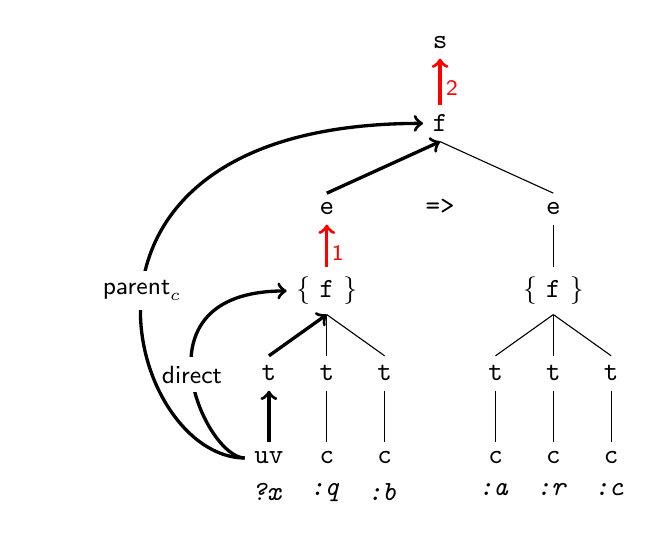
\begin{tikzpicture}
% [
% level 5/.style={level distance=35pt}
% ]
\tikzset{every tree node/.style={align=center,anchor=base}}[sibling distance=150pt]
\Tree [.\texttt{s} \edge[very thick, red,  <-]; [.\node(y){\texttt{f}}; %$\ldots$ 
\edge[very thick,  <-]; 
	[.\node(c){\texttt{e}}; \edge[very thick,  red, <-]; [.\node(a){\{ \texttt{f} \}};   
	               \edge[very thick, <-]; 
	                   [.\texttt{t} \edge[very thick,  <-];  [.\node[label={below:\textit{\texttt{?x}}}](x){\texttt{uv}}; ] ] 
	                   [.\texttt{t} [.\node[label={below:\textit{\texttt{:q}}}]{\texttt{c}}; ] ] 
	                   [.\texttt{t} [.\node[label={below:\textit{\texttt{:b}}}]{\texttt{c}};   ]  ] ] ]
	 \edge[draw=none];  [.\texttt{=>} ] 
	[.\texttt{e} [.{\{ \texttt{f} \}} [.\texttt{t} [.\node[label={below:\textit{\texttt{:a}}}]{\texttt{c}}; ] ] [.\texttt{t} [.\node[label={below:\textit{\texttt{:r}}}]{\texttt{c}}; ] ] [.\texttt{t} [.\node[label={below:\emph{\texttt{:c}}}]{\texttt{c}};  ]  ] ] ]
] ]
%[.\node[label={below:\emph{7}}]{$\texttt{d}^4$}; ]
% \draw[very thick, ->] (x.west)  to  [bend left=90] node [midway,fill=white] {\small{parent}} (y.west);
  \draw[very thick, ->] (x.west)   ..controls +(west:0.5) and +(west:2).. node [midway,fill=white] {\small{direct}} (a.west);
  \draw[very thick, ->] (x.west)..controls +(west:1.5) and +(west:5).. node [midway,fill=white] {\small{$\text{parent}_c$}} (y.west);
   \node[red] (aa) at (-1.3,-2.6) {\footnotesize{1}};
     \node[red] (aaa) at (0.15,-0.5) {\footnotesize{2}};
\end{tikzpicture}\normalsize
\caption{Direct and $\text{parent}_c$ formula. 
% When going through the nodes of the syntax tree from the bottom to the top, the \emph{direct formula} of a component
% \emph{parent formula} of a terminal's direct formula  is
% the formula associated with second node \texttt{f} such that \texttt{f} is a direct child of either an expression \texttt{e}  or the start symbol~\texttt{s}.    
\label{par} }
\end{figure}

To illustrate the idea behind that, we 
%
take  a closer look at one of the concepts used in the informal definitions of \nthree's quantification: %on a concept which is crucial for quantification in \nthree, the concept of parent formulas. %the quantification examples seen so far:
According to the \wwwc team submission~\cite{Notation3} existential variables are quantified on their \emph{direct formula} (Section~\ref{existentials}) and 
universal variables are quantified on their \emph{parent formula} (Section~\ref{universals}). % which therefore need to be identified by a translation mechanism.
%Thus, in order to do a translation from \nthree into core logic, we need to find these
%formulas.
%
%The syntax tree can the concept of 
%To find these two kinds of formulas we can use the syntax tree. %\emph{direct formula} and \emph{parent formula}. 
% which is closely related 
% to quantification in \nthree.
% the behaviour of \nthree's implicit 
% universal quantification as stated in the \wwwc team submission.
%
%
\label{parentformula}
%As discussed in Section~\ref{universals}, implicit universal variables are quantified 
%on the \emph{parent formula} of the formula they \emph{directly occur in}.
Informally 
such a \emph{direct formula} $f$ of a term $t$ is the next formula surrounded by curly brackets \{ \} that contains $t$, or, if such a formula does not exist, 
the top formula. 
In EYE's interpretation, the \emph{parent formula} is now the top formula (concept $\textit{parent}_e$). 
For Cwm, the \emph{parent formula} $g$ of $f$ is the next higher formula surrounded by curly brackets, ie the direct formula of $\{f\}$ ($\textit{parent}_c$). %is a direct component. 
%where \emph{direct} means that  $\{f\}$ is not nested in other \{\}-constructs. 
%
Being the top formula, the $\emph{parent}_e$ \emph{formula} is easy to find. For the \emph{direct formula} and the $\emph{parent}_c$ \emph{formula} we use the syntax tree:
The difference between a simple formula $f$ and a formula in brackets $\{f\}$ is in the grammar point of view the difference between
a \emph{formula} \texttt{f} and a \emph{formula expression}~\texttt{e}.
If we want to find the direct formula of a component and its $\text{parent}_c$, we can go through the syntax tree from the bottom to the top.  
The \emph{direct formula} is then the first formula on that path which is a direct child of either an expression \texttt{e}  or the start symbol~\texttt{s}. 
%ie the 
%first occurrence of a production rule of the form
%$X_0 ::= X_1\ldots X_n$ where $X_0\in \{\texttt{e}, \texttt{s}\}$ and $X_i=\texttt{f}$ for one $i$ with $1\leq i \leq n$.
The $\emph{parent}_c$ \emph{formula} is the second such formula.\footnote{Note that universals on top level like for example in the formula \texttt{?x :p :o.} 
do not have a $\text{parent}_c$. 
We assume here, that these formulas are also quantified on top level. This differs from Cwm which does not support universal quantification on top level.}
%
%
 %Here and in the remainder of this paper we use italic letters to write terminal symbols.
%The parent formula of a universal variable is the second formula (\texttt{f}) we  encounter
%when going up a syntax tree from the node containing the universal to the root. 
%
We illustrate this in Figure~\ref{par} on the syntax tree of the formula:
\begin{equation}
 \texttt{\{?x :q :b\} => \{:a :r :c\}.}\label{for}
\end{equation}
% If we go up the syntax tree from the terminal node \texttt{?x} to the top, we encounter as first formula expression  \texttt{\{?x :q :b.\}}, the formula 
% \texttt{?x :q :b.} is the parent of \texttt{?x}. If we go higher
The direct formula of the terminal node \texttt{?x} is the formula $\texttt{?x :q :b.}$, the
$\text{parent}_c$ formula is the 
top formula. This $\text{parent}_c$ formula carries the universal quantifier for the variable.
 The formula means according to Cwm:
%Thus, the formula means a:
\begin{equation}
\forall \texttt{x. <x q b>}\rightarrow  \texttt{<a r c>.}
 \tag{\ref{for}'}
\end{equation}
Attribute grammars provide a formalism to describe the above process of \emph{going through the syntax tree} in a more precise way. 



\subsection{Attribute Grammars}\label{ag}
\begin{figure}\centering
\begin{tabular}{llclcl}
\hline
\multicolumn{3}{l}{Grammar\hspace*{0.2\textwidth}}&\multicolumn{3}{l}{Synthesized attribute \textit{ds}}\\
%Syntax: &&\\
%&&\\
\hline
\texttt{s ::=}& \texttt{n}&&\texttt{s}.\textit{ds}&$\leftarrow$ & \texttt{n}.\textit{ds}\\
%& \texttt{n}& number\\
 %      &\\
\texttt{n ::= } & %&    \hspace{0.2\textwidth}           numbers:\\  
      \texttt{d} &&  \texttt{n}.\textit{ds} &$\leftarrow$ & %&    \hspace{0.2\textwidth}           numbers:\\  
      \texttt{d}%.\textit{ds}  
      \\%&                digit\\
    &  $\texttt{n}_1 \texttt{n}_2$ &&& $\leftarrow$ & $\texttt{n}_1.\textit{ds} +\texttt{n}_2.\textit{ds}$\\
%\texttt{d ::=}& $i$ with $i\in \{0,1,2,3,4,5,6,7,8,9\}$   \\ 
%\texttt{d ::=}&  \\   
\hline
\end{tabular}
\caption{Context-free grammar producing integers of arbitrary length (left) and definition of the attribute \textit{ds} which composes the digit sum (right). \label{simplegrammar}}
\end{figure}
In this section we give an introduction to attribute grammars~\cite{attributegrammar,ag2}. 
Attribute grammars are defined on top of context-free grammars like the one given above and extend this concept by so-called \emph{attributes}. 
Such attributes 
are defined on the nodes of the syntax tree 
 and can take values.
 These values can depend on other attribute values of the node itself and either its descendent nodes in the syntax tree -- in this case the attribute is called
 \emph{synthesized} -- or 
% they can depend on the node's attributes and 
on the attribute values of the parent node -- in this case it is called \emph{inherited}.
%This formalism is then applied in the following sections to solve, among others, the 
%problem described above.
The definitions used follow the notation of Paakki~\cite{Paakki}.



\subsubsection{Example}
%Before further working with this grammar,
%we use an easier context free grammar to illustrate the idea of attribute grammars. Consider the following context free grammar in  which can be used to generate an integer:
Before providing a formal definition, we illustrate the idea of attribute grammars on a simpler example than the grammar provided above. 
Consider the context-free grammar displayed on the left side of Figure~\ref{simplegrammar}. 
If \texttt{d} can take any value of the alphabet $\mathcal{A}=\{1,2,3,4,5,6,7,8,9,0\}$, %(as a rule $\texttt{d ::= <}\textit{alphabet symbol}{>}$), 
this 
grammar produces integers of arbitrary length.
%
%
%  \begin{figure}
% \begin{tabular}{lcl}
% %Syntax: &&\\
% %&&\\
% \hline
% \texttt{s}.\textit{ds}&$\leftarrow$ & \texttt{n}.\textit{ds}\\
% %& \texttt{n}& number\\
% \texttt{n}.\textit{ds} &$\leftarrow$ & %&    \hspace{0.2\textwidth}           numbers:\\  
%       \texttt{d}  \\%&                digit\\
%     & $\leftarrow$ & \texttt{n}.\textit{ds} +\texttt{n}.\textit{ds}\\
% %\texttt{d}.\textit{ds}&$\leftarrow$ & $i$\\ 
% %\texttt{d ::=}&  \\   
% \hline
% \end{tabular}
% \caption{Rules for the attribute \textit{ds} which produces the digit sum for integers generated by the grammar in Figure~\ref{simplegrammar}. \label{attributeds}}
% \end{figure}
%This grammar can be used to generate an integer of arbitrary length. 
%
A possible\footnote{Note that there are several options to form a tree for 9487, attribute \textit{ds} also computes the digit sum if one of these is chosen.} syntax tree for 9487
is displayed in Figure~\ref{simpletree}. % is displayed in Figure~\ref{simpletree}.
%
\begin{figure}
\begin{center}
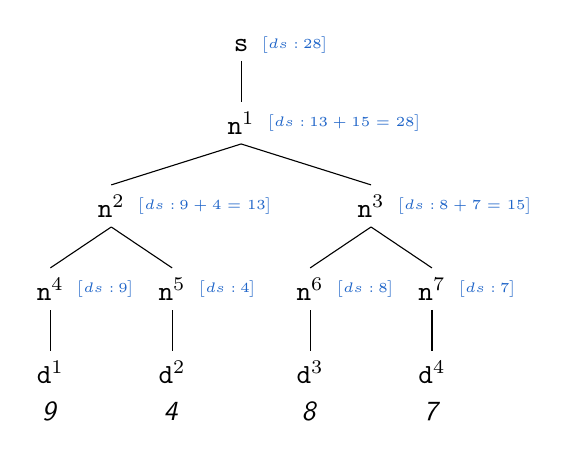
\begin{tikzpicture}
\tikzset{every tree node/.style={align=center,anchor=base}}[sibling distance=300pt]
\Tree [.\node[label={right:\hspace{-0.2cm}\trm{ds:&\hspace{-0.3cm}28}}]{\texttt{s}}; [.\node[label={right:\hspace{-0.2cm}\trm{ds:&\hspace{-0.3cm}13+15=28}}]{$\texttt{n}^1$};
[.\node[label={right:\hspace{-0.2cm}\trm{ds:&\hspace{-0.3cm}9+4=13}}]{$\texttt{n}^2$}; [.\node[label={right:\hspace{-0.2cm}\trm{ds:&\hspace{-0.3cm}9}}]{$\texttt{n}^4$}; 
[.\node[label={below:\emph{9}}]{$\texttt{d}^1$}; ] ] 
[.\node[label={right:\hspace{-0.2cm}\trm{ds:&\hspace{-0.3cm}4}}]{$\texttt{n}^5$}; [.\node[label=below:\emph{4}]{$\texttt{d}^2$}; ] ] ] 
[.\node[label={right:\hspace{-0.2cm}\trm{ds:&\hspace{-0.3cm}8+7=15}}]{$\texttt{n}^3$}; [.\node[label={right:\hspace{-0.2cm}\trm{ds:&\hspace{-0.3cm}8}}]{$\texttt{n}^6$}; 
[.\node[label={below:\emph{8}}]{$\texttt{d}^3$}; ] ] 
[.\node[label={right:\hspace{-0.2cm}\trm{ds:&\hspace{-0.3cm}7}}]{$\texttt{n}^7$}; [.\node[label={below:\emph{7}}]{$\texttt{d}^4$}; ] ] ] ]
]
% \node (b) at (-1.9, -4.1) {} ;
% \node (a) at (-1.9, -3.1) {} ;
% \draw[ugentblue, semithick, ->] (b) to (a);
\end{tikzpicture}
\end{center}
\caption{Syntax tree for 9487 produced by the grammar in Figure~\ref{simplegrammar} 
with attribute values for \emph{ds} (in \color{ugentblue}{\emph{blue}}\color{black}).\label{simpletree}}
\end{figure}
To ease the following discussion, the tree nodes of the same kind are numbered.

If we now want to get the digit sum of an integer produced by that grammar, we can go through the syntax tree from the bottom to the top:
from the nodes resulting in a digit, 
we store that digit. For every node higher in the syntax tree, we take the values of its children and sum them up to a new value. 
Then the values of the start node is the digit sum of 
the integer. 

To formalise this process %of passing information from the bottom of a syntax tree to the top, 
we define the synthesized attribute $\operatorname{\textit{ds}}$. % for all nodes of the syntax tree.
This attribute takes values on each node and these values depend on the production rules of the grammar. 
For each production rule, we define an \emph{attribute rule}.
% For every node $N$ on which an attribute is defined, there are now rules which determine \emph{attribute values} for this node, the \emph{attribute rules}.
% These rules depend on the production rules $X_0 \texttt{ ::= } X_1\ldots X_n$ of the grammar. They can either depend on the rules which have an occurrence of the node on the 
% \emph{right}
% side of 
% the production rule, ie the rules of the form $X_0 \texttt{ ::= } X_1\ldots N \ldots X_n$---in this case they are called \emph{inherited}---%
% or they can depend of the production rules which have the node at the \emph{left} side of the production rule, ie on rules of the form $N \texttt{ ::= } X_1\ldots X_n$---%
% in this case they are called \emph{synthesized}.
% Inherited attributes pass information downwards in the syntax tree, synthesised attributes pass it upwards.
% Since we want the latter, we define our attribute \textit{ds} to be synthesized.
%
% ---in this case they pass information from the top of the syntax tree downwards and are called \emph{inherited}---%
% or they can depend on the rules which have the node on the left hand side---in this case they pass information upwards in the syntax tree and are called \emph{synthesized}. 
% %
%This means that for every node which occurs in a grammar rule there must be a value assigned, the \emph{attribute value}.
%For every node we want to collect in this attribute the digit sum of the number occurring under it.
% for all nodes occurring in the grammar rules.
%In order to pass information from the bottom to the top of the syntax tree as described above, this attribute needs to be \emph{synthesized}.
%Attributes take values for all the nodes they are defined on. %, for a node \texttt{n} and an attribute $a$ we denote that value by $\texttt{n}.a$. 
%These values are determined by so-called \emph{attribute rules}. These are rules which depend on the production rules of the syntax. 
% They can either follow the direction of the 
% production rule---ie define the attribute values of the elements in the body of the production rule based on the attribute values of its head---these are the \emph{inherited} attributes; 
% or they can go in the opposite direction of the production rule---ie define the attribute value of the node in the head of the production rules taking into 
% account the attribute values 
% of the nodes in the body of the rule---these are the \emph{synthesized} attributes. For the process we want to model, we need \textit{ds} to be synthesized since we want to go from the bottom
%to the top of the tree. % ie in the opposite direction of the production rules.
%For our current purpose we need an attribute of the latter kind and let \textit{ds} therefore be synthesized.  
%As our attribute is defined on all nodes, we need to fix one attribute rule for each production rule of the grammar. 
These rules are displayed at the right side
of Figure~\ref{simplegrammar}. 
% Additionally we define that the value $\texttt{d}.\textit{ds}$ is the value of the alphabet symbol connected to \texttt{d} (more formally, we have the grammar 
% rule $\texttt{d ::= <}\textit{alphabet symbol}{>}$ and the attribute rule $\texttt{d}.\textit{ds}\lefttarrow \texttt{<}\textit{alphabet symbol}{>}$).
We denote the attribute value for a node \texttt{n} by \texttt{n}.\textit{ds}. When we use a node resulting in an alphabet symbol of the grammar (in our example \texttt{d}) in an attribute rule,
that symbol refers its alphabet symbol.
Going through the syntax tree from the bottom to the top, we get for 
node $\texttt{n}^4$
%We apply the rules on the syntax tree above. The four terminal nodes have the values:
% $
%  \texttt{d}^1.\textit{ds}=9%;\quad \texttt{d}^2.\textit{ds}= 4;\quad \texttt{d}^3.\textit{ds}= 8;\quad \texttt{d}^4.\textit{ds} = 7
% $
by attribute rule $\texttt{n}.\textit{ds} \leftarrow \texttt{d}$ the value %we get for the nodes $\texttt{n}^4, \texttt{n}^5, \texttt{n}^6$ and $\texttt{n}^7$:
%\[
 $\texttt{n}^4.\textit{ds}=9$. The same rule is used to determine $\texttt{n}^5.\textit{ds}$ to $\texttt{n}^7.\textit{ds}$
 whose values are displayed in Figure~\ref{simpletree}.
%  This is the value 
% of the terminal symbol $\texttt{d}^1$ (9 in this case) upwards to the next node.  
%;\quad \texttt{n}^5.\textit{ds}\leftarrow 4;\quad \texttt{n}^6.\textit{ds}\leftarrow 8;\quad \texttt{n}^7.\textit{ds}\leftarrow 7
%\]
On the next higher level, the attribute value of each node is composed by taking the sum of the attribute values of the direct descendants. This is done by the 
rule $\texttt{n}.\textit{ds}\leftarrow \texttt{n}_1.\textit{ds}+\texttt{n}_2.\textit{ds} $. % bring for the nodes $\texttt{n}^2$ and $\texttt{n}^3$:
We get
 $\texttt{n}^2.\textit{ds}=13$ and
 $\texttt{n}^3.\textit{ds}=15$.
The same rule computes one level higher for $\texttt{n}^1$ the value
$
  \texttt{n}^1.\textit{ds}=28
$
which is then passed to the start node \texttt{s} by the rule $\texttt{s}.\textit{ds}\leftarrow \texttt{n}.\textit{ds}$.
And 28 is indeed the digit sum of 9487.


\subsubsection{Terminology}
% \begin{definition}
% Let  $G=\langle N, \mathcal{A}, P, S\rangle$ be a context free grammar.
% \begin{itemize}
%  \item For each symbol $X\in N\cup \mathcal{A}$ there exists a finite set $A(X)=I(X)\cup S(X)$ of \emph{attributes} with $I(X)\cap S(X) = \emptyset$. We call the set $I(X)$
%  the set of \emph{inherited} attributes and the set $S(X)$ the set of \emph{synthesized} attributes.
%  \item For each left side occurrence $X_0.a$ of a synthesized attribute $a\in S(X)$ in a production rule $p: X_0 \texttt{ ::= } X_1\ldots X_n$ there exists an \emph{attribution rule}
%  \[
%   X.a \leftarrow f(y_1,\ldots, y_k)
%  \]
% where $f$ is a function and $y_i\in A(X_0)\cup A(X_1)\cup\ldots\cup A(X_n)$ for all $1\leq i \leq k$. 
%  \item For each right side occurrence $X_i.a$, $1\leq i \leq n$ of an inherited attribute $a\in I(X)$ in a production rule $p: X_0 \texttt{ ::= } X_1\ldots X_n$ 
%  there exists an \emph{attribution rule}
%  \[
%   X_i.a \leftarrow f(y_1,\ldots, y_k)
%  \]
% where $f$ is a function and $y_i\in A(X_0)\cup A(X_1)\cup\ldots\cup A(X_n)$ for all $1\leq i \leq k$. 
% \end{itemize}
% 
% \end{definition}
%Having seen a concrete example, 
After our example, we now provide a more formal introduction to attribute grammars and fix the terminology we use. 
%
Attribute grammars are defined on top of 
context free grammars
 $G=\langle  N, \mathcal{A}, P, S\rangle$, with $N$ the set of non-terminal symbols,  $\mathcal{A}$ the alphabet or set of terminal symbols, 
$P$ the set of production rules and $S\in N$ a start symbol. 
The set $P$ for the context-free grammar above is displayed in Figure~\ref{simplegrammar}.
This figure also contains all non terminal symbols $N$.
%The alphabet is defined separately and a connection to the alphabet is given by the rule $\texttt{d :: <}\textit{digitsymbol}{>}$.  
The start symbols is \texttt{s}.

For each non-terminal symbol $X\in N$  of the grammar we now define
 a set of attributes $A(X)$. %In our example above, this set of attribute has been for every node $A(X)=\{\textit{ds}\}$.
%
%These attributes are used to pass information through the syntax tree.
%To express that $a\in X$ we use the notation $X.a$.
Each of these attributes either belongs to the set of \emph{inherited} attributes $I(X)$, or to the set of \emph{synthesized} attributes $S(X)$.
%Synthesized attributes are used to pass information from the bottom of a syntax tree to the top like in the example of the previous section, 
%inherited attributes are used for the opposite direction, from the top of a syntax tree to the bottom. 
We assume these two sets of attributes to be disjoint. % $A(X)=I(X)\dot\cup S(X)$.
In our example above we have for each node $X$: $I(X)=\emptyset$, $S(X)=\{\textit{ds}\}$, and $A(X)=\emptyset\cup\{\textit{ds}\}=\{\textit{ds}\}$.
%

To take information, the attributes have assigned values which depend on the production rules they occur in.
%
\begin{definition}[Attribute Occurrence]
Let $G=\langle N, \mathcal{A}, P, S\rangle$ be a context-free grammar and $A:=\bigcup_{X\in N} A(X)$ a set of attributes defined on $N$.
Let $p\in P$
%This assignment depends on the production rules where $X$ occurs in. A rule
be a production rule of the form \[X_0 ::= X_1 \cdots X_n \text{ with } n\geq 1,
\]
\begin{itemize}
\item We say that $p$ has
an \emph{attribute occurrence} $X_i.a$ for the attribute $a$ if $a \in A(X_i)$ for some $i$ with $0\leq i \leq n$.
%\rv{exactly one?}
\item We say that $p$ has a \emph{left-side occurrence}  $X_0.a$ of the attribute $a$, if $a\in A(X_0)$.  
\item We say that $p$ has a \emph{right-side occurrence}  $X_k.a$ of the attribute $a$, if $a\in A(X_k)$ for some $k$ with $1 \leq k \leq n$.
%\rv{exactly one?}
\end{itemize}
\end{definition} 

If we consider another attribute for the grammar in Figure~\ref{simplegrammar}, which is defined only for the node \texttt{d}, the attribute \textit{at},
then the rule
\[
 \texttt{n ::= d} 
\]
has a \emph{right-side occurrence} $\texttt{d}.\textit{at}$ of the attribute \textit{at} while the rule
\[
 \texttt{n ::= n}_1 \texttt{n}_2
\]
does not have any occurrence of \textit{at}.

These occurrences $X_i.a$ now take values, so-called \emph{attribute values}, which are defined by %of a syntezised attribute $X_0.a$ and each occurence of an inherited attribute $X_i.a$, $1\leq i \leq n$, 
 \emph{attribute rules}. These have the form % of the form
\[X_i.a \leftarrow f(y_1\ldots y_n)\]
where $f$ is a function and $y_1\ldots y_n$ are other attribute values. 
An example from above for such an attribute rule is 
\[\texttt{n}.\textit{ds}\leftarrow \texttt{n}_1.\textit{ds}+\texttt{n}_2.\textit{ds} \]
which determines the first occurrence \texttt{n}.\textit{ds} of the attribute \textit{ds} in the production rule
\[
 \texttt{n ::= n}_1 \texttt{n}_2
\]
We denote the set of all
attribute rules for a production rule $p\in P$ by $R(p)$. 
Which exact attribute values can be taken into account when calculating a new attribute value  depends on the kind of attribute:
\begin{definition}[Attribute Grammar]
Let $G=\langle N, \mathcal{A}, P, S\rangle$ be a context-free grammar.
For every element $X\in N$ let $A(X)=I(X)\cup S(X)$ be a finite set of attributes with  $I(X)\cap S(X)=\emptyset$. Let $A=\bigcup_{X\in \mathcal{A}\cup N} A(X)$ 
be the set of all these attributes.
Let  $R=\bigcup_{p\in P} R(p)$ be a finite set of attribute rules.
We call \[AG=\langle G, A, R\rangle\] an \emph{Attribute Grammar} 
if for each production rule $p\in P$ of the form $X_0 \texttt{ ::= } X_1\ldots X_n$ the following holds:
\begin{itemize}
\item for each left-side occurrence $X_0.a$ of a synthesised attribute $a\in S(X_0)$
there exists \emph{exactly one} attribute rule $(X_0.a \leftarrow f(y_1,\ldots,y_k))\in R(p)$ where $f$ is a function and $y_i\in A(X_0)\cup \ldots \cup A(X_n)$ for all $1\leq i \leq k$.
\item for each right-side occurrence $X_i.a$, $1\leq i \leq n$, of an inherited attribute  $a\in I(X_i)$
there exists \emph{exactly one} attribute rule %of the form
$(X_i.a \leftarrow f(y_1,\ldots,y_k))\in R(p)$ where $f$ is a function and $y_j\in A(X_0)\cup \ldots \cup A(X_n)$ for all $1\leq j \leq k$.
\end{itemize}
\end{definition}


%In case of \emph{synthesized attributes} the attribution rules depend on the production rules having the attribute occurrence is on the left side of the rule% 
%the value of an attribute occurrence on the \emph{left} side of a production rule
%is determined taking the attribute values of the right side into account
%---just as we have seen above---% 
%in case of an \emph{inherited attribute} the attribution rules depends on the production rules which have an occurrence on the attribute on the \emph{right}
%side of the rule.
%is determined by taking attribute values of the 
%left hand side into account.
% Above we have seen a synthesized attribute, the attribution rules depended on the production rules carrying the attributed symbol on the left side. In our example, 
% the value of attribute \textit{ds} only depended on the attribute value of \textit{ds} on other nodes. 
% The values can also depend on values of other attributes,
% %These values do not need to be from the same attribute. 
% Note that the attribute value does not only need to depend on  occurrences of the same attribute on different nodes, it could also depend on other values.
% If we for example define our attribute \textit{at} on the node \texttt{d} from above as inherited, a possible attribute rule 
% for the occurrence of the attribute in the rule \texttt{n ::= d} could be:
% \[
%  \texttt{d}.\textit{at} \leftarrow \texttt{n}.\textit{ds}+5
% \]
%or any other value which only depends on attribute values of \texttt{n}.

% Note that the definition states that \emph{inherited} attributes are defined on attribute occurence
% of the right hand side of a rule and \emph{synthesized} attributes are output of the left hand side.
In terms of a syntax tree generated by the grammar synthesized and inherited attributes have exactly the properties mentioned above:  
inherited attributes pass information \emph{down} in the syntax tree, synthesized attributes pass information \emph{upwards}.
We assume the values of synthesized attributes for terminal symbols to be defined externally. The start symbol cannot take an inherited attribute.\footnote{The attentive
reader might have noticed another difference in the structure of the context-free grammar of the core logic (Figure~\ref{syntax}) and the syntax of \nthree (Figure~\ref{N3S}):
the latter has an extra start symbol. The reason for this is rather technical: the attribute grammar we define in the following sections makes use of inherited attributes
defined on the symbol \texttt{f}. Such attributes cannot be defined on a start symbol.
} 


\subsection{Definition of an N3 Attribute Grammar}
\begin{figure}\centering
\begin{tabular}{llll}
\hline
name \hspace*{0.1\textwidth}& type \hspace*{0.1\textwidth}
& defined for \hspace*{0.1\textwidth} &purpose \\
 \hline
 $\eq$ & syn  & $ N$& existentials\\
 \\
 $v_1$ & syn &$ N$& universals in Cwm \\
 $v_2$ & syn &$ N$ & universals in Cwm\\
 $s$ & inh &$\{\texttt{f}, \texttt{t},\texttt{e}, \texttt{k}\}$& universals in Cwm \\
  $q$ & inh &$\{\texttt{f}\}$& universals in Cwm \\
  \\
  $u$ & syn &$ N$& universals in EYE \\
  \\
  $m_c$ & syn  &$ N$& translation Cwm\\
  $m_e$ &syn &$ N$& translation EYE \\
  \hline
\end{tabular}
\caption{Overview of all attributes defined in the \nthree-attribute grammar. The type can be \emph{syn} for synthesized or \emph{inh} for inherited. \label{attributes}}
\end{figure}

After the definition of attribute grammars in the previous section, 
%Having introduced attribute grammars in the previous section, 
we now apply this concept to 
formalise the different interpretations of implicit quantification for \nthreelogic. 
The context-free grammar of \nthree is given in Figure~\ref{N3S} which also contains all symbols of~$N$. The alphabet is given in Definition~\ref{alphabet}. 
The start symbol is~\texttt{s}.

On top of this grammar we now define an attribute grammar in order to be able to produce the two different translations %
of an \nthree formula in core logic, one according to Cwm and the team submission and the other according to EYE.
As a first step we define the sets of attributes for all symbols $X\in N$.
% For all $X\in (N\cup \mathcal{X})\setminus \{\texttt{f}, \texttt{s}\}$ these are 
% \[
%  S(X)=\{\eq, v_1, v_2, u, m_c, m_e\} \text{ and } I(X)=\{s\}
% \]
% For \texttt{s} these are 
% \[
%  S(\texttt{s})=\{\eq, v_1, v_2, u, m_c, m_e\} \text{ and } I(\texttt{s})=\emptyset
% \]
% For \texttt{f} these are
% \[
%  S(\texttt{f})=\{\eq, v_1, v_2, u, m_c, m_e\} \text{ and } I(\texttt{f})=\{s, q\}
% \]
These are displayed in Figure~\ref{attributes}. 
For each of these attributes we also indicated the purpose or context they are used for. This context can be grouped in four parts:  the collection of the variables which are existentially 
quantified under a (sub-)formula (1), the collection
of the universal variables quantified under a (sub-)formula -- once for Cwm (2) and once for EYE (3) -- and attributes to construct the concrete 
expression in core logic which is the translation of the \nthree 
formula dependent on the reasoner (4).
In the following we will go through these four groups one by one, explain the need for the different attributes and provide their definition. We start with attribute $\eq$, which is used for existential scoping. 
%We will explain and define these attributes in this and the following sections.
%We begin with the attribute 
%for existential variables.

\subsubsection{Existentials}\label{exsec}
% tree without labels
% \begin{figure}
% \begin{center}
% \begin{tikzpicture}
% \tikzset{every tree node/.style={align=center}}[sibling distance=140pt]
% \Tree [.\texttt{s} [.\node{$\texttt{f}^1$}; %$\ldots$
% 	[.\node{$\texttt{t}^1$}; [.\node[label={below:\textit{\texttt{\_:x}}}]{$\texttt{ex}^1$}; ] ]          
% 	    % [.t [.\node(x)[label={right: \footnotesize{$v_1=\{\texttt{\textit{?x}}\}$}}]{\texttt{uv}\\{\textit{\texttt{?x}}}}; ] ]  [.t [.\texttt{c}\\{\textit{\texttt{:q}}} ] ] [.t [.\texttt{c}\\{\textit{\texttt{:b}}}   ]  ] ] ]
% 	[.$\texttt{t}^2$ [.\node[label={below:\textit{\texttt{:s}}}]{$\texttt{c}^1$}; ] ] 
% 	[.$\texttt{t}^3$ [.\node(e){\texttt{e}}; [.\node(a){\{$\texttt{f}^2$\}}; 
% 	    [.\node{$\texttt{t}^4$}; [.\node(z)[label={below:\textit{\texttt{\_:y}}}]{$\texttt{ex}^2$}; ] ] 
% 	    [.$\texttt{t}^5$ [.\node[label={below:\textit{\texttt{:k}}}]{$\texttt{c}^2$}; ] ] 
% 	    [.$\texttt{t}^6$ [.\node[label={below:\textit{\texttt{:a}}}]{$\texttt{c}^3$};  ]  ] ] ]
% ] ] ]
% 
%  %\draw[semithick, ->] (z) to  [bend left=90] node [midway,fill=white] {direct} (a);
%  %\draw[semithik, ->] (z) to [bend left=80]  node [midway,fill=white] {$\operatorname{uv}_2=\{\texttt{?x}\}$} (a);
%  %\draw[semithik, ->] (a) to [bend left=80]  node [midway,fill=white] {$\operatorname{sc}=\{\texttt{?x}\}$} (b);
% \end{tikzpicture}\normalsize
% \end{center}
% \caption{Syntax tree for Formula~\ref{eq99}. \label{extreesimple} }
% \end{figure}

% \begin{figure}
% \begin{center}
% \begin{tikzpicture}[
% every tree node/.style={align=center},
% %sibling distance=1cm,
% %level distance =100pt,
% level 2/.style={level distance=40pt},
% level 5/.style={level distance=40pt}
% ]
% \Tree [.\node[label={right:\tr{$\texttt{s}.\eq=\emptyset$}}]{\texttt{s}}; [.\node[label={right:\tr{$\texttt{f}^1.\eq=\{\texttt{\_:x}\}$}}]{$\texttt{f}^1$}; %$\ldots$
% 	[.\node[label={right:\tr{$\texttt{t}^1.\eq=\{\texttt{\_:x}\}$}}]{$\texttt{t}^1$}; [.\node[label={below:\textit{\texttt{\_:x}}}]{$\texttt{ex}^1$}; ] ]          
% 	    % [.t [.\node(x)[label={right: \footnotesize{$v_1=\{\texttt{\textit{?x}}\}$}}]{\texttt{uv}\\{\textit{\texttt{?x}}}}; ] ]  [.t [.\texttt{c}\\{\textit{\texttt{:q}}} ] ] [.t [.\texttt{c}\\{\textit{\texttt{:b}}}   ]  ] ] ]
% 	[.\node[label={right:\tr{$\texttt{t}^2.\eq=\emptyset$}}]{$\texttt{t}^2$}; [.\node[ label={below:\textit{\texttt{:s}}}]{$\texttt{c}^1$}; ] ] 
% 	[.\node[label={right:\tr{$\texttt{t}^3.\eq=\emptyset$}}]{$\texttt{t}^3$}; [.\node(e)[label={right:\tr{$\texttt{e}.\eq=\emptyset$}}]{\texttt{e}}; [.\node(a)[label={right:\tr{$\texttt{f}^2.\eq=\{\texttt{\_:y}\}$}}]{\{$\texttt{f}^2$\}}; 
% 	    [.\node[label={right:\tr{$\texttt{t}^4.\eq=\{\texttt{\_:y}\}$}}]{$\texttt{t}^4$}; [.\node(z)[label={below:\textit{\texttt{\_:y}}}]{$\texttt{ex}^2$}; ] ] 
% 	    [.\node[label={right:\tr{$\texttt{t}^5.\eq=\emptyset$}}]{$\texttt{t}^5$}; [.\node[label={below:\textit{\texttt{:k}}}]{$\texttt{c}^2$}; ] ] 
% 	    [.\node[label={right:\tr{$\texttt{t}^6.\eq=\emptyset$}}]{$\texttt{t}^6$}; [.\node[label={below:\textit{\texttt{:a}}}]{$\texttt{c}^3$};  ]  ] ] ]
% ] ] ]
% \end{tikzpicture}\normalsize
% \end{center}
% \caption{Syntax tree for Formula~\ref{eq99} with values for the attribute $\eq$ (in \tr{blue}). \label{extreesimple} }
% \end{figure}

% tree with long names
% \begin{figure}
% \begin{center}
% \begin{tikzpicture}[
% every tree node/.style={align=center},
% sibling distance=-0.1cm,
% %level distance =100pt,
% level 2/.style={level distance=40pt},
% level 5/.style={level distance=40pt}
% ]
% \linespread{0.5}
% \Tree [.\node[label={right:\tr{$\texttt{s}.\eq=\emptyset$}}]{\texttt{s}}; [.\node[label={right:\tr{$\texttt{f}^1.\eq=\{\texttt{\_:x}\}$}}]{$\texttt{f}^1$}; %$\ldots$
% 	[.\node[label={[align=right]right:{\vspace{3cm}\tr{$\texttt{t}^1.\eq=\{\texttt{\_:x}\}$}}}]{$\texttt{t}^1$}; [.\node[label={below:\textit{\texttt{\_:x}}}]{$\texttt{ex}^1$}; ] ]          
% 	    % [.t [.\node(x)[label={below: \footnotesize{$v_1=\{\texttt{\textit{?x}}\}$}}]{\texttt{uv}\\{\textit{\texttt{?x}}}}; ] ]  [.t [.\texttt{c}\\{\textit{\texttt{:q}}} ] ] [.t [.\texttt{c}\\{\textit{\texttt{:b}}}   ]  ] ] ]
% 	[.\node[label={[align=left] right:\tr{$\texttt{t}^2.\eq=\emptyset$}\hspace{-1cm}}]{$\texttt{t}^2$}; [.\node[ label={below:\textit{\texttt{:s}}}]{$\texttt{c}^1$}; ] ] 
% 	[.\node[label={right:\tr{$\texttt{t}^3.\eq=\emptyset$}}]{$\texttt{t}^3$}; [.\node(e)[label={right:\tr{$\texttt{e}.\eq=\emptyset$}}]{\texttt{e}}; [.\node(a)[label={left:\tr{$\texttt{f}^2.\eq=\{\texttt{\_:y}\}$}}]{\{$\texttt{f}^2$\}}; 
% 	    [.\node[label={[font=\footnotesize, align=center]  left:\hspace{-1.5cm}\tr{$\texttt{t}^4.\eq=\{\texttt{\_:y}\}$}}]{$\texttt{t}^4$}; [.\node(z)[label={below:\textit{\texttt{\_:y}}}]{$\texttt{ex}^2$}; ] ] 
% 	    [.\node[label={[align=right] left:\tr{$\texttt{t}^5.\eq{}={}\emptyset$}\hspace{-0.1cm}}]{$\texttt{t}^5$}; [.\node[label={below:\textit{\texttt{:k}}}]{$\texttt{c}^2$}; ] ] 
% 	    [.\node[label={[align=right] left:\tr{$\texttt{t}^6.\eq=\emptyset$}\hspace{-0.1cm}}]{$\texttt{t}^6$}; [.\node[label={below:\textit{\texttt{:a}}}]{$\texttt{c}^3$};  ]  ] ] ]
% ] ] ]
% \end{tikzpicture}\normalsize
% \end{center}
% \caption{Syntax tree for Formula~\ref{eq99} with values for the attribute $\eq$ (in \tr{blue}). \label{extreesimple} }
% \end{figure}

\begin{figure}
\begin{center}
\begin{tikzpicture}[
every tree node/.style={align=center},
sibling distance=-0.1cm,
%level distance =100pt,
level 2/.style={level distance=40pt},
level 5/.style={level distance=40pt}
]
\linespread{0.5}
\Tree [.\node[label={right:\hspace{-0.2cm}\trm{eq:&\hspace{-0.3cm}\emptyset}}]{\texttt{s}}; [.\node[label={right:\hspace{-0.2cm}\trm{eq:&\hspace{-0.3cm}\{\texttt{x}\}}}]{$\texttt{f}^1$}; %$\ldots$
	[.\node[label={right:\hspace{-0.2cm}\trm{eq:&\hspace{-0.3cm}\{\texttt{x}\}}}]{$\texttt{t}^1$}; [.\node[label={below:\textit{\texttt{\_:x}}}]{$\texttt{ex}^1$}; ] ]          
	    % [.t [.\node(x)[label={below: \footnotesize{$v_1=\{\texttt{\textit{?x}}\}$}}]{\texttt{uv}\\{\textit{\texttt{?x}}}}; ] ]  [.t [.\texttt{c}\\{\textit{\texttt{:q}}} ] ] [.t [.\texttt{c}\\{\textit{\texttt{:b}}}   ]  ] ] ]
	[.\node[label={right:\hspace{-0.2cm}\trm{eq:&\hspace{-0.3cm}\emptyset}}]{$\texttt{t}^2$}; [.\node[ label={below:\textit{\texttt{:s}}}]{$\texttt{c}^1$}; ] ] 
	[.\node[label={right:\hspace{-0.2cm}\trm{eq:&\hspace{-0.3cm}\emptyset}}]{$\texttt{t}^3$}; [.\node(e)[label={right:\hspace{-0.2cm}\trm{eq:&\hspace{-0.3cm}\emptyset}}]{\texttt{e}}; 
	 [.\node(a)[label={right:\hspace{-0.2cm}\trm{eq:&\hspace{-0.3cm}\{\texttt{y}\}}}]{\{$\texttt{f}^2$\}}; 
	    [.\node[label={right:\hspace{-0.2cm}\trm{eq:&\hspace{-0.3cm}\{\texttt{y}\}}}]{$\texttt{t}^4$}; [.\node(z)[label={below:\textit{\texttt{\_:y}}}]{$\texttt{ex}^2$}; ] ] 
	    [.\node[label={right:\hspace{-0.2cm}\trm{eq:&\hspace{-0.3cm}\emptyset}}]{$\texttt{t}^5$}; [.\node[label={below:\textit{\texttt{:k}}}]{$\texttt{c}^2$}; ] ] 
	    [.\node[label={right:\hspace{-0.2cm}\trm{eq:&\hspace{-0.3cm}\emptyset}}]{$\texttt{t}^6$}; [.\node[label={below:\textit{\texttt{:a}}}]{$\texttt{c}^3$};  ]  ] ] ]
] ] ]
\end{tikzpicture}\normalsize
\end{center}
\caption{Syntax tree for Formula~\ref{eq99} with values for the attribute $\eq$ (in \tr{blue}). \label{extreesimple} }
\end{figure}

% \begin{figure}
% \begin{tabular}{lll}
% \hline
% \multicolumn{2}{l}{production rule} & attribute rule\\
%   \hline
% %Syntax: &&\\
% %&&\\
% \texttt{s ::=}&\texttt{f}& $\texttt{s}.\eq \leftarrow \texttt{f}.\eq$\\
%        &&\\
% \texttt{f ::= } &  $ \texttt{t}_1 \texttt{t}_2 \texttt{t}_3.$&   $ \texttt{f}.\eq \leftarrow \texttt{t}_1.\eq\cup \texttt{t}_2.\eq\cup \texttt{t}_3.\eq$ \\
%     &  $\texttt{e}_1 \texttt{=>}  \texttt{e}_2.$& $\texttt{f}.\eq \leftarrow \texttt{e}_1.\eq\cup \texttt{e}_2.\eq$ \\
% %    &  \texttt{@forAll :u}     & universal quantification\\
% %    &  \texttt{@forSome :u}     & existential quantification\\
%     & $ \texttt{f}_1 \texttt{f}_2$ &                $\texttt{f}.\eq \leftarrow \texttt{f}_1.\eq\cup \texttt{f}_2.\eq$ \\
% &&\\
% \texttt{t ::=}& \texttt{uv}\hspace{0.07\textwidth} &                $\texttt{t}.\eq \leftarrow\emptyset$\\
%             & \texttt{ex} &               $\texttt{t}.\eq \leftarrow \{\texttt{ex}\}$\\
%       & \texttt{c} &               $\texttt{t}.\eq \leftarrow\emptyset$\\
%  %     & \texttt{l} &                literals\\
%       & \texttt{e} &                $\texttt{t}.\eq \leftarrow\texttt{e}.\eq $\\
%       & \texttt{(k)}& $\texttt{t}.\eq \leftarrow\texttt{k}.\eq$\\
%       & \texttt{()}& $\texttt{t}.\eq \leftarrow\emptyset$\\
%       &&\\
% \texttt{k ::=}& \texttt{t}& $\texttt{k}.\eq \leftarrow\texttt{t}.\eq$\\
% &\texttt{t k} & $\texttt{k}.\eq \leftarrow\texttt{t}.\eq\cup\texttt{k}.\eq$\\
% &&\\
% \texttt{e ::=}&\texttt{\{f\}} &                $\texttt{e}.\eq \leftarrow\emptyset$\\
%        &\texttt{\{\}} &  $\texttt{e}.\eq \leftarrow\emptyset$\\
%        &\texttt{false}       &                $\texttt{e}.\eq \leftarrow\emptyset$\\
%   \hline
% \end{tabular}
% \caption{Attribute rules for the synthesized attribute $\eq$ (right) and their corresponding production rules (left) from the \nthree grammar (Figure~\ref{N3S}).\label{EQ}}
% \end{figure}

As we have seen in Section~\ref{existentials} the scope on an implicitly existentially quantified variable is the \emph{direct} formula it occurs in. 
The concept of a \emph{direct formula} has been further explained above: 
the direct formula is either the next formula in curly brackets surrounding the existential variable, or -- in case such a formula does not exist -- the formula as a whole.
To recall the idea, consider the following formula:\footnote{Note that structure-wise this formula follows the same pattern as Formula~\ref{eq1}. 
The names of constants are only shortened to
make the presentation of the formula easier.}
% Version without underbrace
\begin{equation}
\texttt{\_:x :s \{\_:y :k :a.\}.} \label{eq99}
\end{equation}
% \begin{equation}
% \underbrace{\texttt{\_:x :s }\underbrace{\texttt{\{\_:y :k :a.\}}}_{\text{direct formula of} \texttt{\_:y}}.}_{\text{direct formula of} \texttt{\_:x}} \label{eq99}
% \end{equation}
The direct formula of variable \texttt{\_:y} is the sub-formula \texttt{\_:y :k :a.} The direct formula of \texttt{\_:x} is
the formula as a whole.
Translated into core logic the formula means:
\begin{equation}\tag{\ref{eq99}'}\label{eq99'}
 \exists \texttt{x.x s <}\exists \texttt{y.y k a>.}
\end{equation}


% The direct formula of variable \texttt{\_:y} is the sub-formula \texttt{\_:y :k :a.} and this is also the formula which carries the existential quantifier for the variable. The direct formula of \texttt{\_:x} is
% the formula as a whole and that is also the formula on which this variable is quantified.
% Translated into core logic the formula means:
% \begin{equation}\tag{\ref{eq99}'}\label{eq99'}
%  \exists \texttt{x.x s <}\exists \texttt{y.y k a>.}
% \end{equation}
% In Section~\ref{n3synsec} we also discussed the idea of using the syntax tree 
% As discussed in Section~\ref{n3synsec} we can use the syntax tree to find a variable's direct formula. This syntax tree is displayed in Figure~\ref{extreesimple} 
% and we again numbered the different occurrences of the same node. 
% To find the direct formula of an existential variable we can go up from the terminal 
% node the variable occurs in till the node in which the 
%Attribute $\eq$ is now used to 
%We now want to define an attribute whose value is the set of existential variables which are quantified within the same direct formula as the node carrying the attribute and occur under this particular node.
In Section~\ref{n3synsec} we discussed the idea of using the syntax tree to find the direct formula. 
If we go upwards in the syntax tree from the occurrence of an existential variable to the next higher node \texttt{e} or \texttt{s}, 
the child formula \texttt{f} of that node
is the existential's direct formula which thus carries its quantifier. %As an example consider 
The syntax tree for our example, Formula~\ref{eq99}, is displayed in Figure~\ref{extreesimple}. 
Here node $\texttt{f}^2$ is such a node
for \texttt{\_:y}  and node $\texttt{f}^1$ for \texttt{\_:x}.

Attribute $\eq$ is now used in this context to keep track of all existential variables which need to be quantified.
%In order to construct a translation as
%
%under such a direct formula. 
If we do a direct translation
of the symbols of the alphabet as mentioned at the end of Section~\ref{n3synsec} and add existential quantifiers whenever we encounter a direct formula, 
the attribute carries for each node the set of
existential variables which are free (see Definition~\ref{free}) under that node and need to be bound when new existential quantifiers are added.

%For the node $\texttt{f}_1$
%In such a process (which will be further explained in Section~\ref{all})
%Let's assume that the quantifiers are added by an synthesized attribute which does this addition whenever a step from a formula \texttt{f} 
%to either the node \texttt{e} or \texttt{s}
%is done (we explain this in detail in Section~\ref{all}), then the value of this attribute on the node $\texttt{f}_1$ is:
% At the step which adds the quantifiers to a translated formula (this is explained in Section~\ref{all}) the value of the attribute $\eq$ is used to know which existential 
% variables need to be quantified.
%To add the existential quantifiers in the translation, we can then make use of the value of $\eq$ whenever we reach a direct formula.
% For the language element 
% \[
%  \texttt{x s <}\exists \texttt{y.y k a>.}
% \]
% Here the variable \texttt{x} is free while \texttt{y} is bound. The value of $\eq$ contains exactly this variable \texttt{x} and
% the translating process uses this information to produce the Formula~\ref{eq99'} as attribute value for the start node \texttt{s}.
%In the translation process whose attributes are further explained in Section~\ref{all} this will be the 
% value of the translation when performing the step from the formula to a node \texttt{s} or \texttt{e} the existential quantifiers are added for all the existential
% variables which occur freely under the node. This would here lead to Formula~\ref{eq99'}. 
% 
% 
% 
% is following this idea: 
% 
% in order to be able to construct such a Core Logic translation as provided in Formula~\ref{eq99'}
% %form Formula~\ref{eq99} 
% we 
% need to know which variables are existentially quantified under a direct formula. 
% The synthesized attribute is passing existentially quantified variables
% upwards in the syntax tree till they reach their direct formula. When constructing a translation, these variables 
% get bound on that direct formula. 
% They are irrelevant for higher nodes of the syntax tree and are therefore not passed further.
% 
% 
% 
%  
% 
% 
% To be able to
% then also construct a translation, we do not only need to find the formulas which carry quantifiers, we also need to pass the quantified variables to that direct formula. 
% This is the purpose of the synthesized attribute $\eq$  
% 
% 
% to perform the translation from  Formula~\ref{eq99} to Formula~\ref{eq99'}.
% This syntax tree is displayed in Figure~\ref{extreesimple}.
% using an attribute grammar, we need to pass the information which variables are existentially quantified
% under a direct formula
% from the place where the symbol occurs, ie the bottom of the syntax tree, to
% this formula. This is the purpose of the synthesized attribute $\eq$. 
%From a core logic's point of view the attribute value of every node is the set of free (see Definition~\ref{free}) existential variables occurring under that node.
% For each node the value of the attribute represents the set of variables occurring in its descendent nodes
% which are quantified on the same direct formula the node occurs in. From the translations point of view, 
% for every node which does not represent a direct formula the value of $\eq$
% is the set of existential variables which occur as free variables (see Definition~\ref{free}) under that node.
\begin{figure}\centering
\begin{tabular}{lll}
\hline
\multicolumn{2}{l}{production rule\hspace*{0.2\textwidth}} & attribute rule\\
  \hline
%Syntax: &&\\
%&&\\
\texttt{s ::=}&\texttt{f}& $\texttt{s}.\eq \leftarrow \emptyset$\\
%       &&\\
\texttt{f ::= } &  $ \texttt{t}_1 \texttt{t}_2 \texttt{t}_3.$&   $ \texttt{f}.\eq \leftarrow \texttt{t}_1.\eq\cup \texttt{t}_2.\eq\cup \texttt{t}_3.\eq$ \\
    &  $\texttt{e}_1 \texttt{=>}  \texttt{e}_2.$& $\texttt{f}.\eq \leftarrow \texttt{e}_1.\eq\cup \texttt{e}_2.\eq$ \\
%    &  \texttt{@forAll :u}     & universal quantification\\
%    &  \texttt{@forSome :u}     & existential quantification\\
    & $ \texttt{f}_1 \texttt{f}_2$ &                $\texttt{f}.\eq \leftarrow \texttt{f}_1.\eq\cup \texttt{f}_2.\eq$ \\
%&&\\
\texttt{t ::=}& \texttt{uv}\hspace{0.07\textwidth} &                $\texttt{t}.\eq \leftarrow\emptyset$\\
            & \texttt{ex} &               $\texttt{t}.\eq \leftarrow \{\texttt{ex}\}$\\
      & \texttt{c} &               $\texttt{t}.\eq \leftarrow\emptyset$\\
 %     & \texttt{l} &                literals\\
      & \texttt{e} &                $\texttt{t}.\eq \leftarrow\texttt{e}.\eq $\\
      & \texttt{(k)}& $\texttt{t}.\eq \leftarrow\texttt{k}.\eq$\\
      & \texttt{()}& $\texttt{t}.\eq \leftarrow\emptyset$\\
%      &&\\
\texttt{k ::=}& \texttt{t}& $\texttt{k}.\eq \leftarrow\texttt{t}.\eq$\\
&$\texttt{t k}_1$ & $\texttt{k}.\eq \leftarrow\texttt{t}.\eq\cup\texttt{k}_1.\eq$\\
%&&\\
\texttt{e ::=}&\texttt{\{f\}} &                $\texttt{e}.\eq \leftarrow\emptyset$\\
       &\texttt{\{\}} &  $\texttt{e}.\eq \leftarrow\emptyset$\\
       &\texttt{false}       &                $\texttt{e}.\eq \leftarrow\emptyset$\\
  \hline
\end{tabular}
\caption{Attribute rules for the synthesized attribute $\eq$ (right) and their corresponding production rules (left) from the \nthree grammar (Figure~\ref{N3S}).\label{EQ}}
\end{figure}
%
%

Following that idea, we define the attribute rules for $\eq$.
%To better understand this idea, we now define the attribute rules:
As $\eq$ is synthesised % and defined for all nodes of the grammar.
%To formalise the idea above we need to define the attribute rules for $\eq$. As $\eq$ is synthesised and defined on all symbols of the grammar, 
we need to state one attribute rule  for each left-side occurrence of an attribute on a production rule of Figure~\ref{N3S}. 
As the attribute is defined for all nodes, we need one attribute rule for each production rule.
% 
% From the production rules occurring at the bottom of the syntax tree, ie the rules only producing symbols of the alphabet, there is one rule which deserves special attention,
% the production rule (\texttt{t ::= ex}): this rule produces an existential variable which at this point occurs as a free variable since we did not find its direct formula yet. 
% The attibute rule for this production rule ($\texttt{t}.\eq \leftarrow \{\texttt{ex}\}$) collects this existential variable in a sigelton set. 
% For all other rules only resulting in symbols of the alphabet the empty set is assigned by the attribution rule since attribute $\eq$ only collects existentials.
% 
% Most other rules now pass the set of existentials upwards in the syntax tree like for example all rules defined for formulas \texttt{f}. There are two exeptions from this:
% 
% 
% 
These attribute rules are displayed in Figure~\ref{EQ} (right) next to their corresponding production rules (left). 
To illustrate how this attribute works, we added the attribute values for each node to the syntax tree in Figure~\ref{extreesimple}.
We explain these rules by going through the tree %The attribute values for each node of the tree are 
%We 
beginning at the bottom.
%To better understand how the rules work, we compute the attribute values for the nodes of the syntax tree in Figure~\ref{extreesimple}.

The production rule (\texttt{t ::= ex}) results in an existential variable and this variable is not quantified under that node.
%When this rule is applied, there is thus Under the node \texttt{t} whose descendent is produced by this rule, there is thus
%exactly one existential variable occurring freely under that node, the existential \texttt{ex}. 
Therefore, the corresponding attribute rule ($\texttt{t}.\eq \leftarrow \{\texttt{ex}\}$) collects this variable in a singleton set 
(values $\texttt{t}^1.\eq$ and $\texttt{t}^4.\eq$). 
%we have the attribute rule .
%For $\texttt{t}^1$ and $\texttt{t}^4$ we get: %whose rule (\texttt{t~::=~ex}) produces existential variables we get via $\texttt{t}.\eq \leftarrow \{\texttt{ex}\}$:
%\[
% \texttt{t}^1.\eq \leftarrow \{\texttt{ex}\}=\{\texttt{\_:x}\}\quad \text{and} \quad  \texttt{t}^4.\eq \leftarrow\{\texttt{ex}\}= \{\texttt{\_:y}\}
%\]
%Here the attribute value stores the existential variable occurring under the node for which the direct formula has not been found yet. 
The attribute rules for other production rules directly resulting in only symbols of the alphabet do not pass any values since there are
no free existential variables occurring under them. 
For the applications of \texttt{t ::= c} %in our syntax tree we get via 
the attribute rule
%
 $\texttt{t}\leftarrow \emptyset$ assigns the empty set to the nodes $\texttt{t}^2$, $\texttt{t}^5$ and $\texttt{t}^6$.
% \[
%  \texttt{t}^2.\eq \leftarrow \emptyset; \quad  \texttt{t}^5.\eq \leftarrow \emptyset;\quad  \texttt{t}^6.\eq \leftarrow \emptyset
% \]
Most other rules now pass the variables from the descendant nodes up to the parents. 
The attribute value  of a
 formula node \texttt{f} 
is the union of its descendants' values. For $\texttt{f}^2$ that is the set $\{\texttt{\_:y}\}$.
% For the production rule ($\texttt{f ::= t}_1 \texttt{t}_2 \texttt{t}_3$) 
% we have the attribute rule $\texttt{f}.\eq \leftarrow \texttt{t}_1.\eq\cup \texttt{t}_2.\eq \cup \texttt{t}_3.\eq$ and get for $\texttt{f}^2$:
% \[
%  \texttt{f}^2 \leftarrow \texttt{t}^4.\eq\cup \texttt{t}^5.\eq\cup \texttt{t}^6.\eq= \{\texttt{\_:y}\}\cup \emptyset \cup \emptyset = \{\texttt{\_:y}\}
% \]
The only exceptions for this behaviour of passing the variables upwards can be found on the attribute rules for the production rules \texttt{s ::= f} 
and \texttt{e ::= \{f\}}. 
As discussed above, the child formulas \texttt{f} of 
\texttt{e} or \texttt{s} are \emph{direct formulas}. % and can thus carry existential quantifiers. 
All free existential variables occurring 
under such direct formulas get bound on these formulas. The attribute rules for \texttt{s ::= f} 
and \texttt{e ::= \{f\}} thus do  not pass any variables upwards. 
%and assign the empty set as
%attribute value. 
% The attribute rule for $\texttt{f}_2$'s parent now deserves special attention. If the production rule (\texttt{e ::= \{f\}}) is applied, we know that \texttt{f} is a 
% \emph{direct formula}, all free existentially quantified variables occurring under the node \texttt{f} are bound by existential quantifiers on this formula in the translation. 
% The attribute rule does thus not pass any existential variable to the parent node. % and has the form $\texttt{e}\leftarrow \emptyset$. 
The attribute value for node \texttt{e} in our syntax tree is the empty set.
% \[
%  \texttt{e}.\eq\leftarrow \emptyset
% \]
This value is again passed upwards via the attribute rule $\texttt{t}.\eq\leftarrow \texttt{e}.\eq$ % for the production rule (\texttt{t ::= e}):
% \[
% \texttt{t}^3.\eq\leftarrow \texttt{e}.\eq= \emptyset 
% \]
and can the be used to determine the attribute value for $\texttt{f}_1$
which is again the union of all its direct descendants' 
values ($\texttt{f}^2.\eq = \{\texttt{\_:x}\}$).
% , again by applying the rule $\texttt{f}.\eq \leftarrow \texttt{t}_1.\eq\cup \texttt{t}_2.\eq \cup \texttt{t}_3.\eq$:
% \[
%  \texttt{f}^2 \leftarrow \texttt{t}^1.\eq\cup \texttt{t}^2.\eq\cup \texttt{t}^3.\eq= \{\texttt{\_:x}\}\cup \emptyset \cup \emptyset = \{\texttt{\_:x}\}
% \]
This node is again a direct formula, it is the child node of the node \texttt{s}. All existential variables are thus bound on $\texttt{f}^2$, the attribute rule does not pass
existential variables upwards. %We get:
%Similarly to the production rule for a formula expression, the attribute rule for the production rule (\texttt{s ::= f}) 
%does not pass any value since the existential variables are bound on this direct formula, we get:
% \[
%  \texttt{s}\leftarrow \emptyset
% \]
%Having for every attribute the set of existentials occurring as free variables under the node enables 

The attribute value of $\eq$ is always the set of free existential variables occurring under a node. For the formulas $\texttt{f}^1$ 
and $\texttt{f}^2$ these are the sets $\texttt{\{\_:x\}}$ and $\texttt{\{\_:y\}}$, respectively. These are exactly the variables existentially quantified on these formulas as can be seen in 
Formula~\ref{eq99'}.
%Of course it is not enough to simply keep track of the existential variables which are free under a node in the syntax tree. 
%We also need to know which variables are universally quantified under each direct formula. This is the topic of the next sections.

% For the existential nodes we get via $\texttt{ex}.\eq$:
% 
% These nodes carry existential variables whose direct formula is not found yet. 
% The rules for the term nodes \texttt{t} are all used to pass information upwards
% 
% 

% \begin{figure}
% \begin{tabular}{rcl}
%   \hline
% %Syntax: &&\\
% %&&\\
% $\texttt{s}.\eq$ & $\leftarrow$ & $\texttt{f}.\eq$\\
%        &&\\
% $ \texttt{f}.\eq$&$ \leftarrow$ & $\texttt{t}_1.\eq\cup \texttt{t}_2.\eq\cup \texttt{t}_3.\eq$ \\
%  $\texttt{f}.\eq$ &  $\leftarrow$ & $\texttt{e}_1.\eq\cup \texttt{e}_2.\eq$ \\
% %    &  \texttt{@forAll :u}     & universal quantification\\
% %    &  \texttt{@forSome :u}     & existential quantification\\
%               $\texttt{f}.\eq$ & $\leftarrow$ & $\texttt{f}_1.\eq\cup \texttt{f}_2.\eq$ \\
% &&\\
%                 $\texttt{t}.\eq$ & $\leftarrow$ &$\emptyset$\\
%            $\texttt{t}.\eq$& $\leftarrow$ & $ \{\texttt{ex}\}$\\
%              $\texttt{t}.\eq$ &$\leftarrow$ & $ \emptyset$\\
%  %     & \texttt{l} &                literals\\
%               $\texttt{t}.\eq$ & $  \leftarrow$ & $ \texttt{e}.\eq $\\
%   $\texttt{t}.\eq$ & $  \leftarrow$ & $ \texttt{k}.\eq$\\
% $\texttt{t}.\eq$ & $  \leftarrow$ & $ \emptyset$\\
%       &&\\
% $\texttt{k}.\eq $ & $ \leftarrow$ & $ \texttt{t}.\eq$\\
%  $\texttt{k}.\eq $ & $ \leftarrow$ & $ \texttt{t}.\eq\cup\texttt{k}.\eq$\\
% &&\\
%               $\texttt{e}.\eq $ & $  \leftarrow$ & $ \emptyset$\\
%    $\texttt{e}.\eq $ & $ \leftarrow$ & $ \emptyset$\\
%                 $\texttt{e}.\eq $ & $ \leftarrow$ & $ \emptyset$\\
%   \hline
% \end{tabular}
% \caption{Attribute rules for the synthesized attribute $\eq$ defined on  the \nthree grammar in Figure~\ref{N3S}.\label{EQsimple}}
% \end{figure}

% 
% The attribute rules which correspond to production rules only resulting in symbols of the 
% alphabet---these are the rules (\texttt{t ::= uv}), (\texttt{t ::= ex}), (\texttt{t ::= c}), (\texttt{t ::= ()}), (\texttt{e ::= \{\}}) and (\texttt{e ::= false})---%
% all produce the empty set as attribute value with one exception:
% For \[\texttt{t ::= ex}
% \text{\quad we define \quad }
%  \texttt{t}.\eq\leftarrow\{\texttt{ex}\}
% \]
% This rule passes every existential variable upwards in the syntax tree. Most of the remaining rules now pass the information they receive from their descendent nodes upwards in the syntax tree. The only rule which does 
% not follow this schema is the rule 
% \[
%  \texttt{e ::= \{f\}}
% \]
% since this rule has a special role:  by passing this rule in the syntax tree we go from the direct formula to the parent formula (see also Section~\ref{n3synsec}). In the translation to Core Logic the formula \texttt{f}
% in this rule carries an existential quantifier which bounds all existential variables freely occurring under it. The corresponding attribute rule
% \[
%  \texttt{e}.\eq \leftarrow \emptyset
% \]
% thus does not pass any existential variable upwards in the syntax tree. We illustrated this situation in Figure~\ref{extree} where we display the syntax tree for Formula~\ref{eq99} together with its attribute values.
% For the nodes which do not have values displayed, the value is always $\emptyset$.
% 
% 
% % From a more declarational point of view, for each node this attribute carries the information which variables occurring  under that node are existentially quantified within the same direct formula the node occurs in. 
% % If we already look from the translation, these are the existential variables which are free in the core logic point of view (see Definition~\ref{free})
% \begin{figure}
% \begin{center}
% \begin{tikzpicture}
% \tikzset{every tree node/.style={align=center,anchor=base}}[sibling distance=140pt]
% \Tree [.s [.\node[label={left: \footnotesize{ $\eq=\{\texttt{\textit{x}}\}$}}]{f}; %$\ldots$
% 	[.\node[label={right: \footnotesize{ $\eq=\{\texttt{\textit{x}}\}$}}]{t}; [.\node[label={right: \footnotesize{$\eq=\{\texttt{\textit{x}}\}$}}]{ex\\\textit{\texttt{\_:x}}}; ] ]          
% 	    % [.t [.\node(x)[label={right: \footnotesize{$v_1=\{\texttt{\textit{?x}}\}$}}]{\texttt{uv}\\{\textit{\texttt{?x}}}}; ] ]  [.t [.\texttt{c}\\{\textit{\texttt{:q}}} ] ] [.t [.\texttt{c}\\{\textit{\texttt{:b}}}   ]  ] ] ]
% 	[.t [.c\\\textit{\texttt{:s}} ] ] 
% 	[.t [.\node[label={left: \footnotesize{ $\eq=\emptyset$}}](e){e}; [.\node[label={left: \footnotesize{ $\eq=\{\texttt{\textit{y}}\}$}}](a){\{f\}}; [.\node[label={left: \footnotesize{ $\eq=\{\texttt{\textit{y}}\}$}}]{t}; [.\node[label={left: \footnotesize{ $\eq=\{\texttt{\textit{y}}\}$}}](z){\texttt{ex}\\{\textit{\texttt{\_:y}}}}; ] ] [.t [.\texttt{c}\\{\textit{\texttt{:k}}} ] ] [.t [.\texttt{c}\\{\textit{\texttt{:a}}}  ]  ] ] ]
% ] ] ]
% \node (xy) at (0.6,-6) {} ;
% \node (x) at (0.85,-5.15) {} ;
% \node (xx) at (1.5,-4.1) {} ;
% \node (xxx) at (1.6,-3.1) {} ;
% \node (y) at (-1.5,-2.9) {};
% \node (a) at (-1.7,-2) {};
% \node (b) at (-0.8, -1) {};
%  \draw[thik, dashed, ->] (xy) to    (x);
%  \draw[thik, dashed, ->] (x) to    (xx);
%   \draw[thik, dashed, ->] (y) to    (a);
%     \draw[thik, dashed, ->] (a) to    (b);
%         \draw[thik, dashed, ->] (xx) to  node {\ding{55}}  (xxx);
%  %\draw[semithick, ->] (z) to  [bend left=90] node [midway,fill=white] {direct} (a);
%  %\draw[semithik, ->] (z) to [bend left=80]  node [midway,fill=white] {$\operatorname{uv}_2=\{\texttt{?x}\}$} (a);
%  %\draw[semithik, ->] (a) to [bend left=80]  node [midway,fill=white] {$\operatorname{sc}=\{\texttt{?x}\}$} (b);
% \end{tikzpicture}\normalsize
% \end{center}
% \caption{Syntax tree for Formula~\ref{eq99} with attribute $\eq$. Attribute $\eq$ is used to pass existentially quantified variables up to their direct formula.
% \todo{new?}
% \label{extree} }
% \end{figure}

% translate implicit existential quantification of \nthree into the explicit quantification of the core logic, 
% we need one attribute which passes all existentially quantified variables occurring under such a direct formula to that formula. 
% That is the purpose of the attribute $\eq$.


% In this subsection we focus on existential quantification and show how the information 
% which variables are quantified on which formula can be stored in attributes. In the following section we do the same for universal variables to 
% then in the subsequent section
% provide further insight how, put together, this leads to concrete core logic translations of \nthree formulas.
% 
% As discussed before, existential variables are quantified on their direct formula. To pass the information which variables are existentially quantified
% on it to such a direct formula we define the synthesized attribute $\eq$ for all symbols $X\in N\cup T$ of our \nthree grammar displayed in Figure~\ref{N3S}. 
% For each production rule
% we now define attribute rules:
% \begin{itemize}
%  \item
% For terminal rules $X ::= Y$, $Y \in T$:
% \[
% X.\eq \leftarrow \begin{cases}
%                   Y,& \text{if}\ X=\texttt{ex}\\
%                   \emptyset, & \text{else}
%                  \end{cases}
% \]
% %with $\operatorname{id}: T\rightarrow T$ being the identity function. 
% \item For the rule $\texttt{e} ::= \texttt{\{f\}}$ we define:
% \[
%  \texttt{e}.\eq \leftarrow \emptyset
% \]
% 
% \item
% For all other rules $X_0 ::= X_1 \ldots X_n$ with $X_i\neq \texttt{e}$ for all $i$ and $X_j\in N$ for at least one $j$, $1\leq i, j \leq n$:
% \[
% X_0.\eq\leftarrow \bigcup_{1\leq j\leq n} X_j.\eq
% \]
% \end{itemize}
% The attribute $\eq$ passes all existentially quantified attributes up in the syntax tree till the direct formula is found, from the direct formula upwards, 
% no variables are passed. We illustrate this in Figure~\ref{extree} where we display the syntax tree for  
% Formula~\ref{eq99}.
% From the rules only resulting in symbols of the alphabet, ie the first three production rules for terms \texttt{t}, only the secod
% \footnote{Note that structure-wise this formula follows the same pattern as Formula~\ref{eq1}. The names of constants are only shortened to
% make the presentation of the formula easier.}
% \begin{equation}
% \texttt{\_:x :s \{\_:y :k :a\}.} \label{eq998}
% \end{equation}
% Translated into core logic this formula means:



%

%
% To produce translations, we need an inherited attribute on \texttt{f} which detects that a formula is a direct formula, ie it either directly follows the start symbol or 
% is part of a formula expression. 
% To understand this, consider the following formula:
% \begin{equation}
%  \texttt{\_:x :p :a. \_:x :q :b.}
% \end{equation}
% 
%  To produce a translation, we additionally need to mark the formulas which can carry a quantifier, the direct formulas. 
%  This is done by the translation attributes which will be introduced in Section~\ref{all}.%These are all formulas \texttt{f} 


%\subsection{Universals}


% \begin{figure*}
% %\begin{minipage}{0.95\textwidth}
% \begin{center}
% \begin{tikzpicture}[%level distance=38pt, %sibling distance=3pt,
% ]
% \tikzset{every tree node/.style={align=center}}%,anchor=base}}
% \Tree [.{\texttt{s}} % \node [ draw, label={[align=left]First\\Second}] {Node}; 
% 	  [.\node%[label={ right: \footnotesize{$v_2=\{\texttt{\textit{x}}\}$, $s=\{\texttt{\textit{x}}\}$, $q=\{\texttt{\textit{x}}\}$}}]
% 	  (a){$\texttt{f}^1$}; 
% 	             [.\node%[label={right: \footnotesize{$v_2=\emptyset$, $s=\{\texttt{\textit{x}}\}$}}]
%            (b){$\texttt{e}^1$}; 
%              [.\{$\texttt{f}^2$\}
%                 [.\node%[label={left: \footnotesize{$v_1=\emptyset$}}, label={right: \footnotesize{$v_2=\{\texttt{\textit{x},\texttt{\textit{y}}}\}$, $s=\{\texttt{\textit{x}},\texttt{\textit{y}}\}$,}}]
%                  {$\texttt{e}^3$}; %$\ldots$
% 	           [.\node%[label={right: \footnotesize{ $\quad v_2=\{\texttt{\textit{x}}, \texttt{\textit{y}}\}$,}}]% $s=\{\texttt{\textit{x}}, \texttt{\textit{y}}\}$}}]
% 	            {\{$\texttt{f}^4$\}}; 
% 	               [.\node%[label={right: \footnotesize{$\quad v_1=\{\texttt{\textit{x}},\texttt{\textit{y}}\}$,}}]% $s=\{\texttt{\textit{x}}, \texttt{\textit{y}}\}$}}]
% 	                {$\texttt{t}^4$}; 
% 	                  [.\node%[label={left: \footnotesize{$v_1=\{\texttt{\textit{x}}\},\quad$}}]{t}; [.\node[label={left: \footnotesize{$v_1=\{\texttt{\textit{x}}\},\quad$}}]% $s=\{\texttt{\textit{x}}, \texttt{\textit{y}}\}$}}]
% 	                  {$\texttt{uv}^2$\\{\textit{\texttt{?x}}}}; ] ] 
% 	                  [.$\texttt{t}^5$ [.$\texttt{c}^3$\\{\textit{\texttt{:q}}} ] ] 
% 	                  [.\node%[label={right: \footnotesize{$ v_1=\{\texttt{\textit{y}}\}$,}}]
% 	                  {$\texttt{t}^6$}; [.\node%[label={right: \footnotesize{$ v_1=\{\texttt{\textit{y}}\}$,}}]% $s=\{\texttt{\textit{x}}, \texttt{\textit{y}}\}$}}]
% 	                  {$\texttt{uv}^3$\\{\textit{\texttt{?y}}}}; ] ] ] ]
% 	           \edge[draw=none]; [.\texttt{=>} ] 
% 	           [.\node%[label={left: \footnotesize{$v_2=\{\texttt{\textit{x}}\},\quad$}}]% $s=\{\texttt{\textit{x}}, \texttt{\textit{y}}\}$}}]
% 	             {$\texttt{e}^4$}; 
% 	              [.\node%[label={left: \footnotesize{$v_1=\{\texttt{\textit{x}}\},\quad$}}]% $s=\{\texttt{\textit{x}}, \texttt{\textit{y}}\}$}}]
% 	                {\{$\texttt{f}^5$\}}; 
% 	              [.\node%[label={left: \footnotesize{$v_1=\{\texttt{\textit{x}}\},\quad$}}]
% 	              {$\texttt{t}^7$}; 
% 	              [.\node%[label={left: \footnotesize{$v_1=\{\texttt{\textit{x}}\},\quad$}}]% $s=\{\texttt{\textit{x}}, \texttt{\textit{y}}\}$}}]
% 	                {$\texttt{uv}^4$\\{\textit{\texttt{?x}}}}; ] ] 
% 	              [.$\texttt{t}^8$ [.$\texttt{c}^4$\\{\textit{\texttt{:r}}} ] ] [.$\texttt{t}^9$ [.$\texttt{c}^5$\\{\textit{\texttt{:c}}} ]  ] ]
%     ] 
%  ] ] 
%             \edge[draw=none]; \texttt{=>} 
% 	       [.\node%[label={left: \footnotesize{$v_2=\{\texttt{\textit{x}}\},\quad$}}]%$s=\{\texttt{\textit{x}}\}$}}]
% 	           (z){$\texttt{e}^2$}; 
% 	          [.\node%[label={left: \footnotesize{$v_1=\{\texttt{\textit{x}}\},\quad$}}]% $s=\{\texttt{\textit{x}}\}$}}]
% 	             (x){\{$\texttt{f}^3$\}};  
% 	          [.\node%[label={left: \footnotesize{$v_1=\{\texttt{\textit{x}}\},\quad$}}]
% 	          (11){$\texttt{t}^1$}; 
% 	          [.\node%[label={left: \footnotesize{$v_1=\{\texttt{\textit{x}}\},\quad$}}]
% 	          (y){$\texttt{uv}^1$\\{{\textit{\texttt{?x}}}}}; ] ] 
% 	          [.$\texttt{t}^2$ [.$\texttt{c}^1$\\{\textit{\texttt{:p}}} ] ] [.$\texttt{t}^3$ [.$\texttt{c}^2$\\{\textit{\texttt{:a}}} ]  ] 
% 	        ] 
% 	   ]    
%  ] ]
% ]
%  %  \draw[semithick, <-] (x) to  [bend right=80] node [midway,fill=white] {$\operatorname{uv}_1=\{\texttt{?x}\}$} (y);
% %   \draw[semithick, <-] (z) to  [bend right=80]  (x);
% %   \draw[semithik, ->] (z) to [bend left=80]  node [midway,fill=white] {$\operatorname{uv}_2=\{\texttt{?x}\}$} (a);
% %   \draw[semithik, ->] (a) to [bend left=80]  node [midway,fill=white] {$\operatorname{sc}=\{\texttt{?x}\}$} (b);
% \end{tikzpicture}%\normalsize
% \end{center}
% \caption{Syntax tree for Formula~\ref{ffff}. \label{treeunisimple}}
% %\end{minipage}
% \end{figure*}
%
%
% 
% \begin{figure}
% %\begin{minipage}{0.95\textwidth}
% \begin{center}
% \begin{tikzpicture}[%level distance=38pt, %sibling distance=3pt,
% ]
% \tikzset{every tree node/.style={align=center}}%,anchor=base}}
% \Tree [.{\texttt{s}} % \node [ draw, label={[align=left]First\\Second}] {Node}; 
% 	  [.\node%[label={ right: \footnotesize{$v_2=\{\texttt{\textit{x}}\}$, $s=\{\texttt{\textit{x}}\}$, $q=\{\texttt{\textit{x}}\}$}}]
% 	  (a){$\texttt{f}^1$}; 
% 	       [.\node%[label={left: \footnotesize{$v_2=\{\texttt{\textit{x}}\},\quad$}}]%$s=\{\texttt{\textit{x}}\}$}}]
% 	           (z){$\texttt{e}^1$}; 
% 	          [.\node%[label={left: \footnotesize{$v_1=\{\texttt{\textit{x}}\},\quad$}}]% $s=\{\texttt{\textit{x}}\}$}}]
% 	             (x){\{$\texttt{f}^2$\}};  
% 		      [.\node%[label={left: \footnotesize{$v_1=\{\texttt{\textit{x}}\},\quad$}}]
% 	                 (11){$\texttt{t}^1$}; 
% 					[.\node%[label={left: \footnotesize{$v_1=\{\texttt{\textit{x}}\},\quad$}}]
% 				(y){$\texttt{uv}^1$\\{{\textit{\texttt{?x}}}}}; ] ] 
% 		      [.$\texttt{t}^2$ 	[.$\texttt{c}^1$\\{\textit{\texttt{:p}}} ] ] 
% 		      [.$\texttt{t}^3$ 	[.$\texttt{c}^2$\\{\textit{\texttt{:a}}} ] ] 
% 	          ] 
% 	       ]  
%           % \edge[draw=none]; \texttt{=>}   
%            [.\node%[label={right: \footnotesize{$v_2=\emptyset$, $s=\{\texttt{\textit{x}}\}$}}]
%            (b){$\texttt{e}^2$}; 
%              [.\{$\texttt{f}^3$\}
%                 [.\node%[label={left: \footnotesize{$v_1=\emptyset$}}, label={right: \footnotesize{$v_2=\{\texttt{\textit{x},\texttt{\textit{y}}}\}$, $s=\{\texttt{\textit{x}},\texttt{\textit{y}}\}$,}}]
%                  {$\texttt{e}^3$}; %$\ldots$
% 	           [.\node%[label={right: \footnotesize{ $\quad v_2=\{\texttt{\textit{x}}, \texttt{\textit{y}}\}$,}}]% $s=\{\texttt{\textit{x}}, \texttt{\textit{y}}\}$}}]
% 	            {\{$\texttt{f}^4$\}}; 
% 	               [.\node%[label={right: \footnotesize{$\quad v_1=\{\texttt{\textit{x}},\texttt{\textit{y}}\}$,}}]% $s=\{\texttt{\textit{x}}, \texttt{\textit{y}}\}$}}]
% 	                {$\texttt{t}^4$}; 
% 	                  [.\node%[label={left: \footnotesize{$v_1=\{\texttt{\textit{x}}\},\quad$}}]{t}; [.\node[label={left: \footnotesize{$v_1=\{\texttt{\textit{x}}\},\quad$}}]% $s=\{\texttt{\textit{x}}, \texttt{\textit{y}}\}$}}]
% 	                  {$\texttt{uv}^2$\\{\textit{\texttt{?x}}}}; ] ] 
% 	                  [.$\texttt{t}^5$ [.$\texttt{c}^3$\\{\textit{\texttt{:q}}} ] ] 
% 	                  [.\node%[label={right: \footnotesize{$ v_1=\{\texttt{\textit{y}}\}$,}}]
% 	                  {$\texttt{t}^6$}; [.\node%[label={right: \footnotesize{$ v_1=\{\texttt{\textit{y}}\}$,}}]% $s=\{\texttt{\textit{x}}, \texttt{\textit{y}}\}$}}]
% 	                  {$\texttt{uv}^3$\\{\textit{\texttt{?y}}}}; ] ] ] ]
% 	           \edge[draw=none]; [.\texttt{=>} ] 
% 	           [.\node%[label={left: \footnotesize{$v_2=\{\texttt{\textit{x}}\},\quad$}}]% $s=\{\texttt{\textit{x}}, \texttt{\textit{y}}\}$}}]
% 	             {$\texttt{e}^4$}; 
% 	              [.\node%[label={left: \footnotesize{$v_1=\{\texttt{\textit{x}}\},\quad$}}]% $s=\{\texttt{\textit{x}}, \texttt{\textit{y}}\}$}}]
% 	                {\{$\texttt{f}^5$\}}; 
% 	              [.\node%[label={left: \footnotesize{$v_1=\{\texttt{\textit{x}}\},\quad$}}]
% 	              {$\texttt{t}^7$}; 
% 	              [.\node%[label={left: \footnotesize{$v_1=\{\texttt{\textit{x}}\},\quad$}}]% $s=\{\texttt{\textit{x}}, \texttt{\textit{y}}\}$}}]
% 	                {$\texttt{uv}^4$\\{\textit{\texttt{?x}}}}; ] ] 
% 	              [.$\texttt{t}^8$ [.$\texttt{c}^4$\\{\textit{\texttt{:r}}} ] ] [.$\texttt{t}^9$ [.$\texttt{c}^5$\\{\textit{\texttt{:c}}} ]  ] ]
%     ] 
%  ] ]
%  ] ] ]
% 
%   \node(fv2) at (0,-2.1){\texttt{=>}};
%  %  \draw[semithick, <-] (x) to  [bend right=80] node [midway,fill=white] {$\operatorname{uv}_1=\{\texttt{?x}\}$} (y);
% %   \draw[semithick, <-] (z) to  [bend right=80]  (x);
% %   \draw[semithik, ->] (z) to [bend left=80]  node [midway,fill=white] {$\operatorname{uv}_2=\{\texttt{?x}\}$} (a);
% %   \draw[semithik, ->] (a) to [bend left=80]  node [midway,fill=white] {$\operatorname{sc}=\{\texttt{?x}\}$} (b);
% \end{tikzpicture}%\normalsize
% \end{center}
% \caption{Syntax tree of Formula~\ref{fff}. \label{treeunisimple}}
% %\end{minipage}
% \end{figure}

% % original figure
% \begin{figure}
% %\begin{minipage}{0.95\textwidth}
% \begin{center}
% \begin{tikzpicture}[%level distance=38pt, %sibling distance=3pt,
% ]
% \tikzset{every tree node/.style={align=center}}%,anchor=base}}
% \Tree [.{\texttt{s}}
% 	  [.\node
% 	  (a){$\texttt{f}^1$};
% %start antecedence 
%            [.\node
%            (b){$\texttt{e}^1$}; 
%              [.\{$\texttt{f}^2$\}
%                 [.\node
%                  {$\texttt{e}^3$}; 
% 	           [.\node
%               {\{$\texttt{f}^4$\}}; 
% 	               [.\node    {$\texttt{t}^1$}; 
% 	                  [.\node[label={below:\textit{\texttt{?x}}}]
% 	                  {$\texttt{uv}^1$}; ] ] 
% 	                  [.$\texttt{t}^2$ [.\node[label={below:\textit{\texttt{:q}}}]{$\texttt{c}^1$}; ] ] 
% 	                  [.\node
% 	                  {$\texttt{t}^3$}; [.\node[label={below:\textit{\texttt{?y}}}]
% 	                  {$\texttt{uv}^2$}; ] ] ] ]
% 	           \edge[draw=none]; [.\texttt{=>} ] 
% 	           [.\node
% 	             {$\texttt{e}^4$}; 
% 	              [.\node
% 	                {\{$\texttt{f}^5$\}}; 
% 	              [.\node
% 	              {$\texttt{t}^4$}; 
% 	              [.\node[label={below:\textit{\texttt{?x}}}]
% 	                {$\texttt{uv}^3$}; ] ] 
% 	              [.$\texttt{t}^5$ [.\node[label={below:\textit{\texttt{:r}}}]{$\texttt{c}^2$}; ] ] [.$\texttt{t}^6$ [.\node[label={below:\textit{\texttt{:c}}}]{$\texttt{c}^3$}; ]  ] ]
%              ] 
%     ] ]
% % stop antecedence
% %start ?x :p :a
% 	       [.\node
% 	           (z){$\texttt{e}^2$}; 
% 	          [.\node
% 	             (x){\{$\texttt{f}^3$\}};  
% 		      [.\node
% 	                 (11){$\texttt{t}^7$}; 
% 					[.\node[label={below:{\textit{\texttt{?x}}}}]
% 				(y){$\texttt{uv}^4$}; ] ] 
% 		      [.$\texttt{t}^8$ 	[.\node[label={below:\textit{\texttt{:p}}}]{$\texttt{c}^4$}; ] ] 
% 		      [.$\texttt{t}^9$ 	[.\node[label={below:\textit{\texttt{:a}}}]{$\texttt{c}^5$}; ] ] 
% 	          ] 
%          ]
% %end ?x :p :a
% 	       ]
% ]
%   \node(fv2) at (0,-2.1){\texttt{=>}};
%  %  \draw[semithick, <-] (x) to  [bend right=80] node [midway,fill=white] {$\operatorname{uv}_1=\{\texttt{?x}\}$} (y);
% %   \draw[semithick, <-] (z) to  [bend right=80]  (x);
% %   \draw[semithik, ->] (z) to [bend left=80]  node [midway,fill=white] {$\operatorname{uv}_2=\{\texttt{?x}\}$} (a);
% %   \draw[semithik, ->] (a) to [bend left=80]  node [midway,fill=white] {$\operatorname{sc}=\{\texttt{?x}\}$} (b);
% \end{tikzpicture}%\normalsize
% \end{center}
% \caption{Syntax tree of Formula~\ref{fff}. \label{treeunisimple}}
% %\end{minipage}
% \end{figure}
% 
% \begin{figure}
% %\begin{minipage}{0.95\textwidth}
% \begin{center}
% \begin{tikzpicture}[%level distance=38pt, %sibling distance=3pt,
% level 1/.style={level distance=40pt},
% level 2/.style={level distance=40pt},
% level 3/.style={level distance=40pt},
% level 4/.style={level distance=40pt},
% level 5/.style={level distance=40pt},
% level 6/.style={level distance=40pt},
% ]
% \tikzset{every tree node/.style={align=center}}%,anchor=base}}
% \Tree [.{
% %\trm{v_1:&\hspace{-0.3cm}\emptyset\\v_2:&\hspace{-0.3cm}\emptyset}
% \scriptsize
% \begin{tabular}{|l|l|}
% \hline
% &\texttt{s}\\
% \hline
% $v_1$\hspace{-0.3cm} & $\emptyset$\\
% $v_2$\hspace{-0.3cm}  & $\emptyset$\\
% \hline
% \end{tabular}
% \normalsize
% }
% \edge[draw=none];	  [.\node
% 	  (a){\scriptsize
% \begin{tabular}{|l|l|}
% \hline
% &$\hspace{-0.1cm}\texttt{f}^1$\\
% \hline
% $\hspace{-0.1cm}v_1$\hspace{-0.1cm} & \hspace{-0.1cm}$\emptyset$\\
% $\hspace{-0.1cm}v_2$\hspace{-0.1cm}  &\hspace{-0.1cm}$\emptyset$\\
% $\hspace{-0.1cm}s$\hspace{-0.1cm}  &$\hspace{-0.1cm}\{\texttt{x},\texttt{y}\}\hspace{-0.2cm}$\\
% $\hspace{-0.1cm}q$\hspace{-0.1cm}  &$\hspace{-0.1cm}\{\texttt{x},\texttt{y}\}\hspace{-0.2cm}$\\
% \hline
% \end{tabular}
% \normalsize};
% \edge[draw=none];[.{\scriptsize
% \begin{tabular}{|l|l|l|}
% \hline
% &$\hspace{-0.1cm}\texttt{e}^1$&$\hspace{-0.1cm}\texttt{e}^2$\\
% \hline
% $\hspace{-0.1cm}v_1$\hspace{-0.1cm} & \hspace{-0.1cm}$\emptyset$&$\hspace{-0.1cm}\{\texttt{x},\texttt{y}\}\hspace{-0.2cm}$\\
% $\hspace{-0.1cm}v_2$\hspace{-0.1cm}  &\hspace{-0.1cm}$\emptyset$&$\hspace{-0.1cm}\{\texttt{x},\texttt{y}\}\hspace{-0.2cm}$\\
% $\hspace{-0.1cm}s$\hspace{-0.1cm}  &$\hspace{-0.1cm}\{\texttt{x},\texttt{y}\}\hspace{-0.2cm}$&$\hspace{-0.1cm}\{\texttt{x},\texttt{y}\}\hspace{-0.2cm}$\\
% \hline
% \end{tabular}
% \normalsize}
% %start antecedence 
%        \edge[draw=none];      [.{\scriptsize
% \begin{tabular}{|l|l|}
% \hline
% &$\hspace{-0.1cm}\texttt{f}^2$\\
% \hline
% $\hspace{-0.1cm}v_1$\hspace{-0.1cm} & \hspace{-0.1cm}$\emptyset$\\
% $\hspace{-0.1cm}v_2$\hspace{-0.1cm}  &\hspace{-0.1cm}$\emptyset$\\
% $\hspace{-0.1cm}s$\hspace{-0.1cm}  &$\hspace{-0.1cm}\{\texttt{x},\texttt{y}\}\hspace{-0.2cm}$\\
% $\hspace{-0.1cm}q$\hspace{-0.1cm}  &$\hspace{-0.1cm}\{\texttt{x},\texttt{y}\}\hspace{-0.2cm}$\\
% \hline
% \end{tabular}
% \normalsize}
%     \edge[draw=none]; [.\node{\scriptsize
% \begin{tabular}{|l|l|l|}
% \hline
% &$\hspace{-0.1cm}\texttt{e}^3$&$\hspace{-0.1cm}\texttt{e}^3$\\
% \hline
% $\hspace{-0.1cm}v_1$\hspace{-0.1cm} & \hspace{-0.1cm}$\emptyset$&$\hspace{-0.1cm}\{\texttt{x},\texttt{y}\}\hspace{-0.2cm}$\\
% $\hspace{-0.1cm}v_2$\hspace{-0.1cm}  &\hspace{-0.1cm}$\emptyset$&$\hspace{-0.1cm}\{\texttt{x},\texttt{y}\}\hspace{-0.2cm}$\\
% $\hspace{-0.1cm}s$\hspace{-0.1cm}  &$\hspace{-0.1cm}\{\texttt{x},\texttt{y}\}\hspace{-0.2cm}$&$\hspace{-0.1cm}\{\texttt{x},\texttt{y}\}\hspace{-0.2cm}$\\
% \hline
% \end{tabular}
% \normalsize};
% 	       \edge[draw=none];    [.\node
%               {\scriptsize
% \begin{tabular}{|l|l|}
% \hline
% &$\hspace{-0.1cm}\texttt{f}^4$\\
% \hline
% $\hspace{-0.1cm}v_1$\hspace{-0.1cm} & \hspace{-0.1cm}$\emptyset$\\
% $\hspace{-0.1cm}v_2$\hspace{-0.1cm}  &\hspace{-0.1cm}$\emptyset$\\
% $\hspace{-0.1cm}s$\hspace{-0.1cm}  &$\hspace{-0.1cm}\{\texttt{x},\texttt{y}\}\hspace{-0.2cm}$\\
% $\hspace{-0.1cm}q$\hspace{-0.1cm}  &$\hspace{-0.1cm}\{\texttt{x},\texttt{y}\}\hspace{-0.2cm}$\\
% \hline
% \end{tabular}
% \normalsize}; 
% 	            \edge[draw=none];   [.\node    {
% 	               \scriptsize
% \begin{tabular}{|l|l|l|l|}
% \hline
% &$\hspace{-0.1cm}\texttt{t}^4$&$\hspace{-0.1cm}\texttt{t}^4$&$\texttt{t}^4$\\
% \hline
% $\hspace{-0.1cm}v_1$\hspace{-0.1cm} & \hspace{-0.1cm}$\emptyset$&\hspace{-0.1cm}$\emptyset$&\hspace{-0.1cm}$\emptyset$\\
% $\hspace{-0.1cm}v_2$\hspace{-0.1cm}  &\hspace{-0.1cm}$\emptyset$&\hspace{-0.1cm}$\emptyset$&\hspace{-0.1cm}$\emptyset$\\
% $\hspace{-0.1cm}s$\hspace{-0.1cm}  &$\hspace{-0.1cm}\{\texttt{x},\texttt{y}\}\hspace{-0.2cm}$&\hspace{-0.1cm}$\{\texttt{x}, \texttt{y}\}\hspace{-0.2cm}$&\hspace{-0.1cm}$\{\texttt{x}, \texttt{y}\}\hspace{-0.2cm}$\\
% \hline
% \end{tabular}
% \normalsize 
% 	               };  ]  
% 	                ]  
% 	            \edge[draw=none];  [.\node
% 	                {\scriptsize
% \begin{tabular}{|l|l|}
% \hline
% &$\hspace{-0.1cm}\texttt{f}^5$\\
% \hline
% $\hspace{-0.1cm}v_1$\hspace{-0.1cm} & \hspace{-0.1cm}$\emptyset$\\
% $\hspace{-0.1cm}v_2$\hspace{-0.1cm}  &\hspace{-0.1cm}$\emptyset$\\
% $\hspace{-0.1cm}s$\hspace{-0.1cm}  &$\hspace{-0.1cm}\{\texttt{x},\texttt{y}\}\hspace{-0.2cm}$\\
% $\hspace{-0.1cm}q$\hspace{-0.1cm}  &$\hspace{-0.1cm}\{\texttt{x},\texttt{y}\}\hspace{-0.2cm}$\\
% \hline
% \end{tabular}
% \normalsize}; 
% 	    \edge[draw=none];  [.{\scriptsize
% \begin{tabular}{|l|l|l|l|}
% \hline
% &$\hspace{-0.1cm}\texttt{t}^4$&$\hspace{-0.1cm}\texttt{t}^4$&$\texttt{t}^4$\\
% \hline
% $\hspace{-0.1cm}v_1$\hspace{-0.1cm} & \hspace{-0.1cm}$\emptyset$&\hspace{-0.1cm}$\emptyset$&\hspace{-0.1cm}$\emptyset$\\
% $\hspace{-0.1cm}v_2$\hspace{-0.1cm}  &\hspace{-0.1cm}$\emptyset$&\hspace{-0.1cm}$\emptyset$&\hspace{-0.1cm}$\emptyset$\\
% $\hspace{-0.1cm}s$\hspace{-0.1cm}  &$\hspace{-0.1cm}\{\texttt{x},\texttt{y}\}\hspace{-0.2cm}$&\hspace{-0.1cm}$\{\texttt{x}, \texttt{y}\}\hspace{-0.2cm}$&\hspace{-0.1cm}$\{\texttt{x}, \texttt{y}\}\hspace{-0.2cm}$\\
% \hline
% \end{tabular}
% \normalsize}  ] ]
%     ] ] 
% % stop antecedence
% %start ?x :p :a 
% 	\edge[draw=none];          [.\node
% 	             (x){\scriptsize
% \begin{tabular}{|l|l|}
% \hline
% &$\hspace{-0.1cm}\texttt{f}^4$\\
% \hline
% $\hspace{-0.1cm}v_1$\hspace{-0.1cm} & \hspace{-0.1cm}$\emptyset$\\
% $\hspace{-0.1cm}v_2$\hspace{-0.1cm}  &\hspace{-0.1cm}$\emptyset$\\
% $\hspace{-0.1cm}s$\hspace{-0.1cm}  &$\hspace{-0.1cm}\{\texttt{x},\texttt{y}\}\hspace{-0.2cm}$\\
% $\hspace{-0.1cm}q$\hspace{-0.1cm}  &$\hspace{-0.1cm}\{\texttt{x},\texttt{y}\}\hspace{-0.2cm}$\\
% \hline
% \end{tabular}
% \normalsize};  
% 		      [.\node
% 	                 (11){\scriptsize
% \begin{tabular}{|l|l|l|l|}
% \hline
% &$\hspace{-0.1cm}\texttt{t}^4$&$\hspace{-0.1cm}\texttt{t}^4$&$\texttt{t}^4$\\
% \hline
% $\hspace{-0.1cm}v_1$\hspace{-0.1cm} & \hspace{-0.1cm}$\emptyset$&\hspace{-0.1cm}$\emptyset$&\hspace{-0.1cm}$\emptyset$\\
% $\hspace{-0.1cm}v_2$\hspace{-0.1cm}  &\hspace{-0.1cm}$\emptyset$&\hspace{-0.1cm}$\emptyset$&\hspace{-0.1cm}$\emptyset$\\
% $\hspace{-0.1cm}s$\hspace{-0.1cm}  &$\hspace{-0.1cm}\{\texttt{x},\texttt{y}\}\hspace{-0.2cm}$&\hspace{-0.1cm}$\{\texttt{x}, \texttt{y}\}\hspace{-0.2cm}$&\hspace{-0.1cm}$\{\texttt{x}, \texttt{y}\}\hspace{-0.2cm}$\\
% \hline
% \end{tabular}
% \normalsize}; 
% 					 ] 
% 	          ] 
% %end ?x :p :a
% 	       ]
% ]]
% %  \node(fv2) at (0,-2.1){\texttt{=>}};
%  %  \draw[semithick, <-] (x) to  [bend right=80] node [midway,fill=white] {$\operatorname{uv}_1=\{\texttt{?x}\}$} (y);
% %   \draw[semithick, <-] (z) to  [bend right=80]  (x);
% %   \draw[semithik, ->] (z) to [bend left=80]  node [midway,fill=white] {$\operatorname{uv}_2=\{\texttt{?x}\}$} (a);
% %   \draw[semithik, ->] (a) to [bend left=80]  node [midway,fill=white] {$\operatorname{sc}=\{\texttt{?x}\}$} (b);
% \end{tikzpicture}%\normalsize
% \end{center}
% \caption{Syntax tree of Formula~\ref{fff}. \label{treeunisimple}}
% %\end{minipage}
% \end{figure}

\subsubsection{Universals in Cwm}\label{unicwm}
% \begin{figure}
% \begin{minipage}{\linewidth}
% \begin{center}
% \scriptsize
% \begin{tikzpicture}[scale=.68,
% level distance=70pt, sibling distance=-5pt,
% level 1/.style={level distance=26pt},
% level 2/.style={level distance=50pt},
% level 3/.style={level distance=30pt},
% level 4/.style={level distance=55pt},
% level 5/.style={level distance=30pt},
% level 6/.style={level distance=55pt},
% level 7/.style={level distance=30pt},
% ]
% \tikzset{every tree node/.style={align=base}}%,anchor=base}}
% \Tree [.\node[label={right:\trm{v_1:&\hspace{-0.3cm}\emptyset\\v_2:&\hspace{-0.3cm}\emptyset}}]{\texttt{s}};
% 	  [.\node
% 	  (a)[label={right:{\hspace{0.5cm}\trmv{\emptyset}{\{\texttt{x}\}}{\{\texttt{x}\}}{\{\texttt{x}\}}}
% 		}]{$\texttt{f}^1$};
% %start antecedence 
%            [.\node
%            (b)[label={right:\hspace{0.2cm}\trmd{\emptyset}{\emptyset}{\{\texttt{x}\}}
% 		     }]{$\texttt{e}^1$}; 
%              [.\node[label={right:\hspace{0.1cm}\trmv{\emptyset}{\{\texttt{x}, \texttt{y}\}}{\{\texttt{x}, \texttt{y}\}}{\{\texttt{y}\}}}]{\{$\texttt{f}^2$\}};
%                 [.\node[label={right:\trmd{\emptyset}{\{\texttt{x},\texttt{y}\}}{\{\texttt{x},\texttt{y}\}}
% 		     }]
%                  {$\texttt{e}^3$}; 
% 	           [.\node[label={right:\trmv{\{\texttt{x}, \texttt{y}\}}{\emptyset}{\{\texttt{x}, \texttt{y}\}}{\emptyset}}]
%               {\{$\texttt{f}^4$\}}; 
% 	               [.\node [label={right:\trmd{\{\texttt{x}\}}{\emptyset}{\{\texttt{x}, \texttt{y}\}}
% 		     }]   {$\texttt{t}^1$}; 
% 	                  [.\node[label={below: \textit{\texttt{?x}}}]
% 	                  {$\texttt{uv}^1$}; ] ] 
% 	                  [.\node[label={right:\trmd{\emptyset}{\emptyset}{\{\texttt{x}, \texttt{y}\}}
% 		     }]{$\texttt{t}^2$}; [.\node[label={below:\textit{\texttt{:q}}}]{$\texttt{c}^1$}; ] ] 
% 	                  [.\node[label={right:\trmd{\{\texttt{y}\}}{\emptyset}{\{\texttt{x}, \texttt{y}\}}
% 		     }]
% 	                  {$\texttt{t}^3$}; [.\node[label={below:\textit{\texttt{?y}}}]
% 	                  {$\texttt{uv}^2$}; ] ] ] ]
% 	           \edge[draw=none]; [.\texttt{ } ] 
% 	           [.\node[label={right:\trmd{\emptyset}{\{\texttt{x}\}}{\{\texttt{x}, \texttt{y}\}}
% 		     }]
% 	             {$\texttt{e}^4$}; 
% 	              [.\node[label={right:\trmv{\{\texttt{x}\}}{\emptyset}{\{\texttt{x}, \texttt{y}\}}{\emptyset}}]
% 	                {\{$\texttt{f}^5$\}}; 
% 	              [.\node[label={right:\trmd{\{\texttt{x}\}}{\emptyset}{\{\texttt{x},\texttt{y}\}}
% 		     }]
% 	              {$\texttt{t}^4$}; 
% 	              [.\node[label={below:\textit{\texttt{?x}}}]
% 	                {$\texttt{uv}^3$}; ] ] 
% 	              [.\node[label={right:\trmd{\emptyset}{\emptyset}{\{\texttt{x},\texttt{y}\}}
% 		     }]{$\texttt{t}^5$}; [.\node[label={below:\textit{\texttt{:r}}}]{$\texttt{c}^2$}; ] ] 
% 		     [.\node[label={right:\trmd{\emptyset}{\emptyset}{\{\texttt{x},\texttt{y}\}\hspace{-6cm}}
% 		     }]{$\texttt{t}^6$}; [.\node[label={below:\textit{\texttt{:c}}}]{$\texttt{c}^3$}; ]  ] ]
%              ] 
%     ] ]
% % stop antecedence
% %start x :p :a
% 	       [.\node[label={right:\trmd{\emptyset}{\{\texttt{x}\}}{\{\texttt{x}\}}
% 		     }]
% 	           (z){$\texttt{e}^2$}; 
% 	          [.\node
% 	             (x)[label={right:\trmv{\{\texttt{x}\}}{\emptyset}{\{\texttt{x}\}}{\emptyset}}]{\{$\texttt{f}^3$\}};  
% 		      [.\node
% 	                 (11)[label={right:\trmd{\{\texttt{x}\}}{\emptyset}{\{\texttt{x}\}}
% 		     }]{$\texttt{t}^7$}; 
% 					[.\node
% 				(y)[label={below: {\textit{\texttt{?x}}}}]{$\texttt{uv}^4$}; ] ] 
% 		      [.\node[label={right:\trmd{\emptyset}{\emptyset}{\{\texttt{x}\}}
% 		     }]{$\texttt{t}^8$}; 	[.\node[label={below: \textit{\texttt{:p}}}]{$\texttt{c}^4$}; ] ] 
% 		      [.\node[label={right:\trmd{\emptyset}{\emptyset}{\{\texttt{x}\}}
% 		     }]{$\texttt{t}^9$}; 	[.\node[label={below: \textit{\texttt{:a}}}]{$\texttt{c}^5$}; ] ] 
% 	          ] 
%          ]
% %end ?x :p :a
% 	       ]
% ]
%   \node(fv2) at (0,-2.1){\texttt{=>}};
%   \node(fv3) at (-3.8,-5.3){\texttt{=>}};
% %  \node() at (-4,-9.8){\color{grey}{\texttt{\{ \{ ?x\hspace{1.4cm}:q\hspace{1.4cm}?y \} => \{ ?x\hspace{1.4cm}:r\hspace{1.4cm}:c \} \} => \{ ?x\hspace{1.4cm}:p\hspace{1.4cm}:a \}}}};
%  %  \draw[semithick, <-] (x) to  [bend right=80] node [midway,fill=white] {$\operatorname{uv}_1=\{\texttt{?x}\}$} (y);
% %   \draw[semithick, <-] (z) to  [bend right=80]  (x);
% %   \draw[semithik, ->] (z) to [bend left=80]  node [midway,fill=white] {$\operatorname{uv}_2=\{\texttt{?x}\}$} (a);
% %   \draw[semithik, ->] (a) to [bend left=80]  node [midway,fill=white] {$\operatorname{sc}=\{\texttt{?x}\}$} (b);
% \end{tikzpicture}\normalsize
% \end{center}
% \caption{Syntax tree of Formula~\ref{fff} with attribute values for the attributes $v_1$, $v_2$, $s$ and $q$ (in \tr{blue}). \label{treeunisimple}}
% \end{minipage}
% \end{figure}
%\begin{landscape}
\begin{sidewaysfigure}
\begin{minipage}{\linewidth}
\begin{center}
\scriptsize
\begin{tikzpicture}[
level distance=70pt, sibling distance=-5pt,
level 1/.style={level distance=26pt},
level 2/.style={level distance=50pt},
level 3/.style={level distance=30pt},
level 4/.style={level distance=55pt},
level 5/.style={level distance=30pt},
level 6/.style={level distance=55pt},
level 7/.style={level distance=30pt},
]
\tikzset{every tree node/.style={align=base}}%,anchor=base}}
\Tree [.\node[label={right:\trm{v_1:&\hspace{-0.3cm}\emptyset\\v_2:&\hspace{-0.3cm}\emptyset}}]{\texttt{s}};
	  [.\node
	  (a)[label={right:{\hspace{0.5cm}\trmv{\emptyset}{\{\texttt{x}\}}{\{\texttt{x}\}}{\{\texttt{x}\}}}
		}]{$\texttt{f}^1$};
%start antecedence 
           [.\node
           (b)[label={right:\hspace{0.2cm}\trmd{\emptyset}{\emptyset}{\{\texttt{x}\}}
		     }]{$\texttt{e}^1$}; 
             [.\node[label={right:\hspace{0.1cm}\trmv{\emptyset}{\{\texttt{x}, \texttt{y}\}}{\{\texttt{x}, \texttt{y}\}}{\{\texttt{y}\}}}]{\{$\texttt{f}^2$\}};
                [.\node[label={right:\trmd{\emptyset}{\{\texttt{x},\texttt{y}\}}{\{\texttt{x},\texttt{y}\}}
		     }]
                 {$\texttt{e}^3$}; 
	           [.\node[label={right:\trmv{\{\texttt{x}, \texttt{y}\}}{\emptyset}{\{\texttt{x}, \texttt{y}\}}{\emptyset}}]
              {\{$\texttt{f}^4$\}}; 
	               [.\node [label={right:\trmd{\{\texttt{x}\}}{\emptyset}{\{\texttt{x}, \texttt{y}\}}
		     }]   {$\texttt{t}^1$}; 
	                  [.\node[label={below: \textit{\texttt{?x}}}]
	                  {$\texttt{uv}^1$}; ] ] 
	                  [.\node[label={right:\trmd{\emptyset}{\emptyset}{\{\texttt{x}, \texttt{y}\}}
		     }]{$\texttt{t}^2$}; [.\node[label={below:\textit{\texttt{:q}}}]{$\texttt{c}^1$}; ] ] 
	                  [.\node[label={right:\trmd{\{\texttt{y}\}}{\emptyset}{\{\texttt{x}, \texttt{y}\}}
		     }]
	                  {$\texttt{t}^3$}; [.\node[label={below:\textit{\texttt{?y}}}]
	                  {$\texttt{uv}^2$}; ] ] ] ]
	           \edge[draw=none]; [.\texttt{ } ] 
	           [.\node[label={right:\trmd{\emptyset}{\{\texttt{x}\}}{\{\texttt{x}, \texttt{y}\}}
		     }]
	             {$\texttt{e}^4$}; 
	              [.\node[label={right:\trmv{\{\texttt{x}\}}{\emptyset}{\{\texttt{x}, \texttt{y}\}}{\emptyset}}]
	                {\{$\texttt{f}^5$\}}; 
	              [.\node[label={right:\trmd{\{\texttt{x}\}}{\emptyset}{\{\texttt{x},\texttt{y}\}}
		     }]
	              {$\texttt{t}^4$}; 
	              [.\node[label={below:\textit{\texttt{?x}}}]
	                {$\texttt{uv}^3$}; ] ] 
	              [.\node[label={right:\trmd{\emptyset}{\emptyset}{\{\texttt{x},\texttt{y}\}}
		     }]{$\texttt{t}^5$}; [.\node[label={below:\textit{\texttt{:r}}}]{$\texttt{c}^2$}; ] ] 
		     [.\node[label={right:\trmd{\emptyset}{\emptyset}{\{\texttt{x},\texttt{y}\}\hspace{-6cm}}
		     }]{$\texttt{t}^6$}; [.\node[label={below:\textit{\texttt{:c}}}]{$\texttt{c}^3$}; ]  ] ]
             ] 
    ] ]
% stop antecedence
%start x :p :a
	       [.\node[label={right:\trmd{\emptyset}{\{\texttt{x}\}}{\{\texttt{x}\}}
		     }]
	           (z){$\texttt{e}^2$}; 
	          [.\node
	             (x)[label={right:\trmv{\{\texttt{x}\}}{\emptyset}{\{\texttt{x}\}}{\emptyset}}]{\{$\texttt{f}^3$\}};  
		      [.\node
	                 (11)[label={right:\trmd{\{\texttt{x}\}}{\emptyset}{\{\texttt{x}\}}
		     }]{$\texttt{t}^7$}; 
					[.\node
				(y)[label={below: {\textit{\texttt{?x}}}}]{$\texttt{uv}^4$}; ] ] 
		      [.\node[label={right:\trmd{\emptyset}{\emptyset}{\{\texttt{x}\}}
		     }]{$\texttt{t}^8$}; 	[.\node[label={below: \textit{\texttt{:p}}}]{$\texttt{c}^4$}; ] ] 
		      [.\node[label={right:\trmd{\emptyset}{\emptyset}{\{\texttt{x}\}}
		     }]{$\texttt{t}^9$}; 	[.\node[label={below: \textit{\texttt{:a}}}]{$\texttt{c}^5$}; ] ] 
	          ] 
         ]
%end ?x :p :a
	       ]
]
  \node(fv2) at (0,-2.1){\texttt{=>}};
  \node(fv3) at (-3.8,-5.3){\texttt{=>}};
%  \node() at (-4,-9.8){\color{grey}{\texttt{\{ \{ ?x\hspace{1.4cm}:q\hspace{1.4cm}?y \} => \{ ?x\hspace{1.4cm}:r\hspace{1.4cm}:c \} \} => \{ ?x\hspace{1.4cm}:p\hspace{1.4cm}:a \}}}};
 %  \draw[semithick, <-] (x) to  [bend right=80] node [midway,fill=white] {$\operatorname{uv}_1=\{\texttt{?x}\}$} (y);
%   \draw[semithick, <-] (z) to  [bend right=80]  (x);
%   \draw[semithik, ->] (z) to [bend left=80]  node [midway,fill=white] {$\operatorname{uv}_2=\{\texttt{?x}\}$} (a);
%   \draw[semithik, ->] (a) to [bend left=80]  node [midway,fill=white] {$\operatorname{sc}=\{\texttt{?x}\}$} (b);
\end{tikzpicture}\normalsize
\end{center}
\caption{Syntax tree of Formula~\ref{fff} with attribute values for the attributes $v_1$, $v_2$, $s$ and $q$ (in \tr{blue}). \label{treeunisimple}}
\end{minipage}
\end{sidewaysfigure}
%\end{landscape}

%\begin{landscape}
\begin{sidewaysfigure}
\begin{minipage}{\linewidth}
\begin{center}\small
 \begin{tabular}{llllll}
\hline

\multicolumn{2}{c}{CFG}& \multicolumn{2}{c}{Synthesized attributes} &\multicolumn{2}{c}{Inherited attributes}\\
\multicolumn{2}{l}{production rules}& \multicolumn{1}{l}{rules for $v_1$}&  \multicolumn{1}{l}{rules for $v_2$}& \multicolumn{1}{l}{rules for $s$}& \multicolumn{1}{l}{rules for $q$} \\
  \hline
%Syntax: &&\\
%&&\\
\texttt{s ::=}&\texttt{f}& $\texttt{s}.v_1 \leftarrow \emptyset$& $\texttt{s}.v_2 \leftarrow \texttt{f}.v_1$& $\texttt{f}.s \leftarrow \texttt{f}.v_1\cup \texttt{f}.v_2$& $\texttt{f}.q\leftarrow \texttt{f}.v_1 \cup \texttt{f}.v_2$\\
       &&&&\\
\texttt{f ::= } &  $ \texttt{t}_1 \texttt{t}_2 \texttt{t}_3.$&   $ \texttt{f}.v_1 \leftarrow \texttt{t}_1.v_1\cup \texttt{t}_2.v_1\cup \texttt{t}_3.v_1$ & $ \texttt{f}.v_2 \leftarrow \texttt{t}_1.v_2\cup \texttt{t}_2.v_2\cup \texttt{t}_3.v_2$& $\texttt{t}_i.s \leftarrow \texttt{f}.s$ \\
    &  $\texttt{e}_1 \texttt{=>}  \texttt{e}_2.$& $\texttt{f}.v_1 \leftarrow \texttt{e}_1.v_1\cup \texttt{e}_2.v_1$ & $\texttt{f}.v_2 \leftarrow \texttt{e}_1.v_2\cup \texttt{e}_2.v_2$& $\texttt{e}_i.s\leftarrow \texttt{f}.s$ \\
%    &  \texttt{@forAll :u}     & universal quantification\\
%    &  \texttt{@forSome :u}     & existential quantification\\
    & $ \texttt{f}_1 \texttt{f}_2$ &                $\texttt{f}.v_1 \leftarrow \texttt{f}_1.v_1\cup \texttt{f}_2.v_1$ &   $\texttt{f}.v_2 \leftarrow \texttt{f}_1.v_2\cup \texttt{f}_2.v_2$&  $\texttt{f}_i.s\leftarrow \texttt{f}.s$ &$\texttt{f}_i.q \leftarrow \emptyset$  \\
&&&\\
\texttt{t ::=}& \texttt{uv}%\hspace{0.07\textwidth} 
&                $\texttt{t}.v_1 \leftarrow\{ \texttt{uv}\}$ &  $\texttt{t}.v_2 \leftarrow\emptyset$&&\\% $\texttt{uv}.s\leftarrow \texttt{t}.s$\\
            & \texttt{ex} &               $\texttt{t}.v_1 \leftarrow \emptyset$&  $\texttt{t}.v_2 \leftarrow\emptyset$& &\\%$\texttt{ex}.s\leftarrow \texttt{t}.s$\\
      & \texttt{c} &               $\texttt{t}.v_1 \leftarrow\emptyset$&  $\texttt{t}.v_2 \leftarrow\emptyset$& &\\ % $\texttt{c}.s\leftarrow \texttt{t}.s$\\
 %     & \texttt{l} &                literals\\
      & \texttt{e} &                $\texttt{t}.v_1 \leftarrow\texttt{e}.v_1 $ &  $\texttt{t}.v_2 \leftarrow\texttt{e}.v_2 $& $\texttt{e}.s\leftarrow \texttt{t}.s$\\
      & \texttt{(k)}& $\texttt{t}.v_1 \leftarrow\texttt{k}.v_1$ &$\texttt{t}.v_2 \leftarrow\texttt{k}.v_2$& $\texttt{k}.s\leftarrow \texttt{t}.s$\\
      & \texttt{()}& $\texttt{t}.v_1 \leftarrow\emptyset$&  $\texttt{t}.v_2 \leftarrow\emptyset$\\
      &&&\\
\texttt{k ::=}& \texttt{t}& $\texttt{k}.v_1 \leftarrow\texttt{t}.v_1$ & $\texttt{k}.v_2 \leftarrow\texttt{t}.v_2$& $\texttt{t}.s\leftarrow \texttt{k}.s$\\
&$\texttt{t k}_1$ & $\texttt{k}.v_1 \leftarrow\texttt{t}.v_1\cup\texttt{k}_1.v_1$ & $\texttt{k}.v_2 \leftarrow\texttt{t}.v_2\cup\texttt{k}_1.v_2$& $\texttt{t}.s\leftarrow \texttt{k}.s$\\
&&&& $\texttt{k}_1.s\leftarrow \texttt{k}.s$\\
&&&\\
\texttt{e ::=}&\texttt{\{f\}} &                $\texttt{e}.v_1 \leftarrow\emptyset$ &  $\texttt{e}.v_2 \leftarrow\texttt{f}.v_1$& $\texttt{f}.s\leftarrow \texttt{e}.s \cup \texttt{f}.v_2$& $\texttt{f}.q \leftarrow \texttt{f}.v_2 \setminus \texttt{e}.s$\\
       &\texttt{\{\}} &  $\texttt{e}.v_1 \leftarrow\emptyset$ &  $\texttt{e}.v_2 \leftarrow\emptyset$\\
       &\texttt{false}       &                $\texttt{e}.v_1 \leftarrow\emptyset$&                $\texttt{e}.v_2 \leftarrow\emptyset$\\
  \hline

\end{tabular}
\end{center}   \normalsize
\caption{Attribute rules for universal quantification in Cwm defined on the context-free grammar of \nthree (Figure~\ref{N3S}).\label{uniatt}}
\end{minipage}
\end{sidewaysfigure}
%\end{landscape}


% \begin{figure*}
% \begin{minipage}{\textwidth}
% \begin{center}
% \small
% \begin{tikzpicture}[
% level distance=70pt, sibling distance=-5pt,
% level 1/.style={level distance=28pt},
% level 2/.style={level distance=40pt},
% level 3/.style={level distance=35pt},
% level 4/.style={level distance=50pt},
% level 5/.style={level distance=30pt},
% level 6/.style={level distance=50pt},
% level 7/.style={level distance=25pt},
% ]
% \tikzset{every tree node/.style={align=center}}%,anchor=base}}
% \Tree [.\node[label={right:\trm{v_1:&\hspace{-0.3cm}\emptyset\\v_2:&\hspace{-0.3cm}\emptyset}}]{\texttt{s}};
% 	  [.\node
% 	  (a)[label={right:{\trmv{\emptyset}{\{\texttt{x}\}}{\{\texttt{x}\}}{\{\texttt{x}\}}}
% 		}]{$\texttt{f}^1$};
% %start antecedence 
%            [.\node
%            (b)[label={right:\trmd{\emptyset}{\emptyset}{\{\texttt{x}\}}
% 		     }]{$\texttt{e}^1$}; 
%              [.\node[label={right:\trmv{\emptyset}{\{\texttt{x}, \texttt{y}\}}{\{\texttt{x}, \texttt{y}\}}{\{\texttt{y}\}}}]{\{$\texttt{f}^2$\}};
%                 [.\node[label={right:\trmd{\emptyset}{\{\texttt{x},\texttt{y}\}}{\{\texttt{x},\texttt{y}\}}
% 		     }]
%                  {$\texttt{e}^3$}; 
% 	           [.\node[label={right:\trmv{\{\texttt{x}, \texttt{y}\}}{\emptyset}{\{\texttt{x}, \texttt{y}\}}{\emptyset}}]
%               {\{$\texttt{f}^4$\}}; 
% 	               [.\node [label={right:\trmd{\{\texttt{x}\}}{\emptyset}{\{\texttt{x}, \texttt{y}\}}
% 		     }]   {$\texttt{t}^1$}; 
% 	                  [.\node[label={below: \textit{\texttt{?x}}}]
% 	                  {$\texttt{uv}^1$}; ] ] 
% 	                  [.\node[label={right:\trmd{\emptyset}{\emptyset}{\{\texttt{x}, \texttt{y}\}}
% 		     }]{$\texttt{t}^2$}; [.\node[label={below:\textit{\texttt{:q}}}]{$\texttt{c}^1$}; ] ] 
% 	                  [.\node[label={right:\trmd{\{\texttt{y}\}}{\emptyset}{\{\texttt{x}, \texttt{y}\}}
% 		     }]
% 	                  {$\texttt{t}^3$}; [.\node[label={below:\textit{\texttt{?y}}}]
% 	                  {$\texttt{uv}^2$}; ] ] ] ]
% 	           \edge[draw=none]; [.\texttt{=>} ] 
% 	           [.\node[label={right:\trmd{\emptyset}{\{\texttt{x}\}}{\{\texttt{x}, \texttt{y}\}}
% 		     }]
% 	             {$\texttt{e}^4$}; 
% 	              [.\node[label={right:\trmv{\{\texttt{x}\}}{\emptyset}{\{\texttt{x}, \texttt{y}\}}{\emptyset}}]
% 	                {\{$\texttt{f}^5$\}}; 
% 	              [.\node[label={right:\trmd{\{\texttt{x}\}}{\emptyset}{\{\texttt{x},\texttt{y}\}}
% 		     }]
% 	              {$\texttt{t}^4$}; 
% 	              [.\node[label={below:\textit{\texttt{?x}}}]
% 	                {$\texttt{uv}^3$}; ] ] 
% 	              [.\node[label={right:\trmd{\emptyset}{\emptyset}{\{\texttt{x},\texttt{y}\}}
% 		     }]{$\texttt{t}^5$}; [.\node[label={below:\textit{\texttt{:r}}}]{$\texttt{c}^2$}; ] ] 
% 		     [.\node[label={right:\trmd{\emptyset}{\emptyset}{\{\texttt{x},\texttt{y}\}\hspace{-6cm}}
% 		     }]{$\texttt{t}^6$}; [.\node[label={below:\textit{\texttt{:c}}}]{$\texttt{c}^3$}; ]  ] ]
%              ] 
%     ] ]
% % stop antecedence
% %start x :p :a
% 	       [.\node[label={right:\trmd{\emptyset}{\{\texttt{x}\}}{\{\texttt{x}\}}
% 		     }]
% 	           (z){$\texttt{e}^2$}; 
% 	          [.\node
% 	             (x)[label={right:\trmv{\emptyset}{\{\texttt{x}\}}{\emptyset}{\emptyset}}]{\{$\texttt{f}^3$\}};  
% 		      [.\node
% 	                 (11)[label={right:\trmd{\{\texttt{x}\}}{\emptyset}{\{\texttt{x}\}}
% 		     }]{$\texttt{t}^7$}; 
% 					[.\node
% 				(y)[label={below: {\textit{\texttt{?x}}}}]{$\texttt{uv}^4$}; ] ] 
% 		      [.\node[label={right:\trmd{\emptyset}{\emptyset}{\{\texttt{x}\}}
% 		     }]{$\texttt{t}^8$}; 	[.\node[label={below: \textit{\texttt{:p}}}]{$\texttt{c}^4$}; ] ] 
% 		      [.\node[label={right:\trmd{\emptyset}{\{\emptyset}{\{\texttt{x}\}}
% 		     }]{$\texttt{t}^9$}; 	[.\node[label={below: \textit{\texttt{:a}}}]{$\texttt{c}^5$}; ] ] 
% 	          ] 
%          ]
% %end ?x :p :a
% 	       ]
% ]
%   \node(fv2) at (0,-2.1){\texttt{=>}};
%  %  \draw[semithick, <-] (x) to  [bend right=80] node [midway,fill=white] {$\operatorname{uv}_1=\{\texttt{?x}\}$} (y);
% %   \draw[semithick, <-] (z) to  [bend right=80]  (x);
% %   \draw[semithik, ->] (z) to [bend left=80]  node [midway,fill=white] {$\operatorname{uv}_2=\{\texttt{?x}\}$} (a);
% %   \draw[semithik, ->] (a) to [bend left=80]  node [midway,fill=white] {$\operatorname{sc}=\{\texttt{?x}\}$} (b);
% \draw[help lines] (-9,-9) grid (7,0);
% \end{tikzpicture}\normalsize
% \end{center}
% \caption{Syntax tree of Formula~\ref{fff} with attribute values for the attributes $v_1$, $v_2$, $s$ and $q$ (in \tr{blue}). \label{treeunisimple}}
% \end{minipage}
%\end{figure*}


The interpretations of \nthree's implicit universal quantification differs between reasoners. 
With a few exceptions\footnote{The developer of Cwm, Tim Berners-Lee, confirmed that these exceptions were not intended
and rather need to be seen as mistakes in the implementation.}, which we also discuss in Appendix~\ref{bugsincwm}, 
Cwm implements interpretation $\emph{parent}_c$ %(from Sections~\ref{universals} and \ref{parentformula}) 
of the 
concept \emph{parent formula} from the \wwwc team submission while 
for EYE the \emph{parent formula} is the top formula ($\emph{parent}_e$). In this section we explain the concept of $\emph{parent}_c$ in more detail
%how implicit universal quantification is interpreted by the former 
and define attributes to place universal quantifiers according to this concept. 
The details on the interpretation following to EYE are discussed in the next section.
%
% the \wwwc team submission and the reasoners cwm and EYE. 
% We therefore treat them separately and present in this section all 
% attributes we use to handle universal quantification as stated in the \wwwc team submission. With a few exceptions cwm follows the 
% 
% 
% As the interpretations of universally quantified variables differ between %the \wwwc team submission and 
% the reasoners cwm and EYE, we will discuss
% them separately.
% We start with universal quantification according to cwm which directly follows \wwwc team submission.
% \todo{there are exceptions to this ``following the team submission'' should I mention them or consider them as bugs?}

%
%
%
%In Section~\ref{universals} we have already seen an example how implicit universal quantification is handled 


In the previous sections we have seen that in contrast to implicitly existentially quantified variables, 
universals are -- according to the \wwwc team submission -- not quantified on the \emph{direct formula}
but on the \emph{parent}.
%As explained above, according to the \wwwc team submission universal 
%variables are not quantified on their direct formula but on their parent formula. 
%The concept of parent formula has been further explained in
This concept has (at least) two conflicting interpretations which have been further explained in 
Section~\ref{parentformula}. One of them is $\text{parent}_c$:  %A $\text{parent}_e$ formula is the top formula. 
The $\text{parent}_c$ is the direct formula of the direct formula or -- in terms of the syntax tree -- the second descendant \texttt{f} of a node \texttt{s} or 
\texttt{e} we find when going up the syntax tree from the bottom to the top.
In the following formula, for example,
\begin{multline}\label{fff}
\texttt{\{\{?x :q ?y.\} => \{?x :r :c.\}.\} =>}
\texttt{\{?x :p :a.\}.}
\end{multline}
the $\text{parent}_c$ of the last occurrence of \texttt{?x} is the formula as a whole,
the $\text{parent}_c$ of \texttt{?y} is the subformula
\[
 \texttt{ \{?x :q ?y.\} => \{?x :r :c.\}.}
\]
or, if we take a look into the formula's syntax tree displayed in Figure~\ref{treeunisimple}, 
the $\text{parent}_c$ of the last \texttt{?x} ($\texttt{uv}^4$) is $\texttt{f}^1$ and 
the $\text{parent}_c$ of \texttt{?y} ($\texttt{uv}^2$) is
$\texttt{f}^2$. Therefore formula $\texttt{f}^1$ carries a universal quantifier for \texttt{?x} and $\texttt{f}^2$ carries a universal quantifier for \texttt{?y}.
The first universal quantifier also covers the other occurrences of \texttt{?x} since the $\text{parent}_c$ formula of these
other occurrences, namely $\texttt{f}^2$, is already 
in scope of this quantifier. %\todo{explain earlier}
Formula~\ref{fff} means:
\begin{equation}\tag{\ref{fff}'}\label{iall}
 \forall \texttt{x. } \texttt{<} \forall \texttt{y. <x q y>} \rightarrow \texttt{<x r c> >} \rightarrow \texttt{<x p a>}
\end{equation}
Similarly to the example of existential quantification, 
we define attributes which pass universal variables occurring under a $\text{parent}_c$ formula up to that $\text{parent}_c$ formula. 
For this purpose, we use two attributes whose values are as follows:
\begin{description}
 \item[$v_1$]  the set of universal variables occurring as direct components under a node.
 \item[$v_2$]  the set of universal variables occurring as direct components of direct components (parent level).
\end{description}
The first attribute $v_1$ is used to pass universal attributes up to their direct formulas, the second attribute $v_2$ is used to further pass these variables from the direct formulas
to the $\text{parent}_c$ formulas. The attributes are again synthesized and we have one attribute rule for each production rule. These attribute rules are displayed in the second and third 
column of the table in Figure~\ref{uniatt}. The first column of the table shows the corresponding production rules. To better explain the attributes, 
we apply them to the syntax tree
of Formula~\ref{fff}. The tree and the corresponding attribute values are displayed in Figure~\ref{treeunisimple}.


% \begin{tabular}{lcccc}
% \hline
% node & \multicolumn{4}{c}{attribute values}\\
%  &$v_1$&$v_2$&$s$&$q$\\
%  \hline
%  $\texttt{t}^1$& $\{\texttt{?x}\}$&$\emptyset$&&\\
%  $\texttt{t}^2$& $\emptyset$&$\emptyset$&&\\
%  $\texttt{t}^3$& $\{\texttt{?y}\}$&$\emptyset$&&\\
%  $\texttt{t}^4$& $\{\texttt{?x}\}$&$\emptyset$&&\\
%  $\texttt{t}^5$& $\emptyset$&$\emptyset$&&\\
%  $\texttt{t}^6$& $\emptyset$&$\emptyset$&&\\
%  $\texttt{t}^7$& $\{\texttt{?x}\}$&$\emptyset$&&\\
%  $\texttt{t}^8$& $\emptyset$&$\emptyset$&&\\
%  $\texttt{t}^9$& $\emptyset$&$\emptyset$&&\\
%  $\texttt{f}^1$& $\emptyset$&$\{\texttt{?x}\}$&&\\
%  $\texttt{f}^2$& $\emptyset$&$\{\texttt{?x}, \texttt{?y}\}$&&\\
%  $\texttt{f}^3$& $\{\texttt{?x}\}$&$\emptyset$&&\\
%  $\texttt{f}^4$& $\{\texttt{?x}, \texttt{?y}\}$&$\emptyset$&&\\
%  $\texttt{f}^5$& $\{\texttt{?x}\}$&$\emptyset$&&\\
%  $\texttt{e}^1$& $\emptyset$&$\emptyset$&&\\
%  $\texttt{e}^2$& $\emptyset$&$\{\texttt{?x}\}$&&\\
%  $\texttt{e}^3$& $\emptyset$&$\{\texttt{?x}, \texttt{?y}\}$&&\\
%  $\texttt{e}^4$& $\emptyset$&$\{\texttt{?x}\}$&&\\
%  $\texttt{s}$& $\emptyset$&$\emptyset$&&\\
% \end{tabular}


\subsubsection*{Passing Variables to their Direct Formula}
Attribute $v_1$ works the exact same way as attribute $eq$ with the only difference that at term level the universals
get captured in a singleton set ($\texttt{t}.v_1\leftarrow\{\texttt{uv}\}$)  instead of the existentials. These universals are then passed upwards to their $\text{parent}_c$ formulas.
% In our example, formula $\texttt{f}^4$ is the parent formula of the first occurrence of \texttt{?x} and of \texttt{?y}, $\texttt{f}^5$ and $\texttt{f}^3$ are the parents of the other 
% occurrences of \texttt{?x}. 
In our example, the formulas $\texttt{f}^1$ and $\texttt{f}^2$ do not have universal variables as direct components, $\texttt{f}^3$ has \texttt{?x}, $\texttt{f}^4$ has \texttt{?x} and \texttt{?y},
and 
formula $\texttt{f}^5$ has \texttt{?x}.
% We start with attribute $v_1$. Similarly to attribute $\eq$ from the previous section, the attribute is used to pass direct components 
% up to their direct formula, the only difference
% between the two attributes is that $v_1$ collects universals instead of existentials. Via the attribute rule $\texttt{t}.v_1\leftarrow \{\texttt{uv}\}$ on the production rule
% (\texttt{t ::= uv}) we get:
% \begin{align}\notag
%  \texttt{t}^1.v_1\leftarrow \{\texttt{uv}^1\}=\{\texttt{?x}\}; \qquad \texttt{t}^3.v_1\leftarrow \{\texttt{uv}^2\}=\{\texttt{?y}\}; \\ 
%  \texttt{t}^4.v_1\leftarrow \{\texttt{uv}^3\}=\{\texttt{?x}\}; \qquad \texttt{t}^7.v_1\leftarrow \{\texttt{uv}^4\}=\{\texttt{?x}\}. \notag
% \end{align}
% The universal variable occur directly under the nodes \texttt{t}, there is no node \texttt{e} or \texttt{s} in between. As for $\eq$ all nodes directly resulting in 
% only other symbols of the alphabet get assigned the empty set as value. Via the rule $\texttt{t}.v_1\leftarrow~\emptyset$ on the rule (\texttt{t ::= c}) we get:
% \begin{align*}\notag
%  \texttt{t}^2.v_1\leftarrow \emptyset; \qquad \texttt{t}^5.v_1\leftarrow \emptyset; \qquad \texttt{t}^6.v_1\leftarrow \emptyset; \\ 
%  \texttt{t}^8.v_1\leftarrow \emptyset; \qquad \texttt{t}^9.v_1\leftarrow \emptyset. \notag
% \end{align*}
% These values are passed upwards via the attribute rule $\texttt{f}.v_1\leftarrow \texttt{t}_1.v_1\cup\texttt{t}_2.v_1\cup \texttt{t}_3.v_1$ on the production rule
% $\texttt{f ::= t}_1 \texttt{t}_2 \texttt{t}_3$:
% \small
% \begin{align}\notag
% \texttt{f}^4.v_1 & \leftarrow \texttt{t}^1.v_1 \cup \texttt{t}^2.v_1\cup \texttt{t}^3.v_1=\{\texttt{?x}\}\cup \emptyset \cup \{\texttt{?y}\} = \{\texttt{?x,?y}\};\\
% \notag \texttt{f}^5.v_1& \leftarrow \texttt{t}^4.v_1 \cup \texttt{t}^5.v_1\cup \texttt{t}^6.v_1=\{\texttt{?x}\}\cup \emptyset \cup \emptyset = \{\texttt{?x}\};\\
% \notag \texttt{f}^3.v_1& \leftarrow \texttt{t}^7.v_1 \cup \texttt{t}^8.v_1\cup \texttt{t}^9.v_1=\{\texttt{?x}\}\cup \emptyset \cup \emptyset = \{\texttt{?x}\};
% \end{align}
% \normalsize
% As in the previous example, most rules behave like that with two exceptions: the attribute rules for the production rules having \texttt{e} or \texttt{s} in their 
% head do not pass the variables upwards since
% on these nodes the variables are no longer direct components, their direct formula is the descendant node \texttt{f}. We get via $\texttt{e}\leftarrow \emptyset$ for
% (\texttt{e~::=~\{f\}}):
% \[
%  \texttt{e}^3.v_1\leftarrow \emptyset; \qquad  \texttt{e}^4.v_1\leftarrow \emptyset; \qquad  \texttt{e}^2.v_1\leftarrow \emptyset;
% \]
% The attribute value on each higher node is now the empty set:
% \begin{align}\nonumber
%  &\texttt{f}^2.v_1 \leftarrow \texttt{e}^3.v_1 \cup \texttt{e}^4.v_1 = \emptyset \cup \emptyset =\emptyset; \quad
%  \texttt{e}^1.v_1 \leftarrow \emptyset;\notag \\
%   &\texttt{f}^1.v_1 \leftarrow \texttt{e}^1.v_1 \cup \texttt{e}^2.v_1 = \emptyset \cup \emptyset =\emptyset; \quad
%    \texttt{s}.v_1 \leftarrow \emptyset\notag 
% \end{align}
% The formulas $\texttt{f}^1$ and $\texttt{f}^2$ do not have universal variables as direct components, $\texttt{f}^3$ has \texttt{?x}, $\texttt{f}^4$ has \texttt{?x} and \texttt{?y},
% and 
% formula $\texttt{f}^5$ has \texttt{?x}.

\subsubsection*{Passing Variables to their Parent Formula}
Attribute $v_2$ now passes  the universal variables which are collected under their direct formula using  $v_1$ to their $\text{parent}_c$ formula.
%, we need another attribute, $v_2$. 
This attribute works in a similar way as the previous one:
at the level where the universal variables of a direct formula \texttt{f} under a node \texttt{e} are found the rule for the synthesized attribute 
takes these values gathered by the attribute $v_1$ and 
passes them upwards till the next formula being 
direct descendant of a node \texttt{s} or \texttt{e} is encountered. This formula is then the $\text{parent}_c$.
%
% While 
% attribute $v_1$ keeps track of the universal variables occurring as direct components in a formula, attribute $v_2$ performs the next step: 
% all variables which occur in a formula expressions 
%In terms of the explanation given at the end of Section~\ref{n3synsec}, 
%
%This attribute is again defined for all nodes.
% 
% To make sure that we know for each parent formula the set of universal variables it is parent of, we need to have an attribute which passes the universal variable directly occurring 
% in a formula's direct formula expression to that formula.
% In terms of the explanation at the end of Section~\ref{n3synsec}, %and the illustration in Figure~\ref{par},
% attribute $v_1$ captures the set of variables which---going from the bottom of the syntax tree to the top---have arrived at the first formula \texttt{f} being direct descendant
%  of a node \texttt{e} or \texttt{s}, attribute
%  $v_2$ is used to capture the second time a value reaches such a node \texttt{f}.

We display the rules for attribute $v_2$ in the third column of Figure~\ref{uniatt}. 
We explain the rules by going through the syntax tree in Figure~\ref{treeunisimple} from the bottom to the top. %The tree contains all attribute values for our example.
The rules only resulting in symbols of the alphabet cannot have direct components. %the attribute values for the nodes  are the empty set.
The attribute rule $\texttt{t}.v_2\leftarrow \emptyset$ for the production rules \texttt{t~::=~uv} and \texttt{t~::=~c} assign the empty set to the term nodes
$\texttt{t}^1$ to $\texttt{t}^9$.
% \begin{align}
%  &\notag \texttt{t}^1.v_2 \leftarrow \emptyset; \quad \texttt{t}^2.v_2 \leftarrow \emptyset; \quad \texttt{t}^3.v_2  \leftarrow \emptyset; 
%  \\
%  &\notag \texttt{t}^4.v_2  \leftarrow \emptyset;\quad \texttt{t}^5.v_2  \leftarrow \emptyset;\quad  \texttt{t}^6.v_2 \leftarrow \emptyset;
%  \\
%  &\notag \texttt{t}^7.v_2 \leftarrow \emptyset; \quad \texttt{t}^8.v_2 \leftarrow \emptyset; \quad \texttt{t}^9.v_2 \leftarrow \emptyset
% \end{align}
These values are passed upwards via the attribute rule $\texttt{f}\leftarrow \texttt{t}_1.v_2\cup \texttt{t}_2.v_2 \cup \texttt{t}_3.v_2$ 
on production rule $\texttt{f ::= t}_t \texttt{t}_2 \texttt{t}_3$, 
the attribute values for $\texttt{f}^3$, $\texttt{f}^4$ and $\texttt{f}^5$ are again the empty set.
% \[
%  \texttt{f}^3.v_2\leftarrow \emptyset; \quad \texttt{f}^4.v_2\leftarrow \emptyset; \quad \texttt{f}^5.v_2\leftarrow \emptyset
% \]
The attribute rule for the next higher level, the production \texttt{e ::= \{f\}} is more interesting. 
The variables which occur as direct components on the formula node \texttt{f} and are captured by the attribute $v_1$
are passed as children of the next $\text{parent}_c$ formula to the node \texttt{e} via the attribute rule $\texttt{e}.v_2\leftarrow \texttt{f}.v_1$. We get: 
$\texttt{e}^2.v_2 =\{\texttt{?x}\}$,
$\texttt{e}^3.v_2 =\{\texttt{?x}, \texttt{?y}\}$ and
$\texttt{e}^4.v_2 =\{\texttt{?x}\}
$.
For $\texttt{f}^2$ these values are passed upwards via the attribute rule $\texttt{f}\leftarrow \texttt{e}_1 \cup \texttt{e}_2$.
% (
%  $\texttt{f}^2.v_2\leftarrow\{\texttt{?x}, \texttt{?y}\}$
% )
As $\texttt{f}^2$ is a direct descendant  of the node $\texttt{e}^1$, it is the $\text{parent}_c$ formula of the variables mentioned above. 
These variables are not passed further through. Instead, the attribute value for $\texttt{e}^1$ is again taken from the attribute $v_1$
(via $\texttt{e}.v_2\leftarrow \texttt{f}.v_1$) which in this case is the empty set.
% \[
%  \texttt{e}^1.v_2\leftarrow \texttt{f}^2.v_1= \emptyset
% \]
With these values we can determine the attribute value for $\texttt{f}^1$ (via $\texttt{f}\leftarrow \texttt{e}_1 \cup \texttt{e}_2$) which in this case is 
the singleton set only containing the variable \texttt{?x}.
% \[
%  \texttt{f}^1.v_2\leftarrow \texttt{e}^1.v_2\cup\texttt{e}^2.v_2=\emptyset \cup \{\texttt{?x}\} = \{\texttt{?x}\}
% \]
The attribute value for \texttt{s} is the empty set. 

For formulas which are direct descendants of a node \texttt{s} or \texttt{e} the value is now the set of universal variables for which the formula is a $\text{parent}_c$:
for $\texttt{f}^1$ that is $\{\texttt{?x}\}$, for $\texttt{f}^2$ it is $\{\texttt{?x}, \texttt{?y}\}$, and for $\texttt{f}^3$, $\texttt{f}^4$ and $\texttt{f}^5$ 
the value is the empty set since these formulas are not 
$\text{parent}_c$ formulas. 

% Considering the fact that universal variables are quantified on their parent formula, we would expect the meaning of Formula~\ref{fff} to be:
% \begin{multline}\notag
%   \forall \texttt{x. < x p a>}\rightarrow\\
%  \texttt{<} \forall \texttt{x.}\forall \texttt{y. < x q y>} \rightarrow \texttt{< x r c> >}^*
% \end{multline}
% But if we look again to the interpretation given earlier in Formula~\ref{iall} this is not the case.
% Formula $\texttt{f}^3$ does not carry a quantifier for \texttt{x} in the interpretation. 
% The reason for that is that variable \texttt{x} is already quantified: $\{\texttt{f}^3\}$ is a direct component of the formula $\texttt{f}^1$ which already carries a quantifier for \texttt{?x}. 
% In the interpretation according to the \wwwc team submission, this quantifier also covers 
% all nested occurrences of of the variable under that same formula thus also for \texttt{?x} under $\texttt{f}^3$.%

%With this result and the knowledge that universal variables are quantified on their parent formula we go back to the interpretation of Formula~\ref{fff}. 

\subsubsection*{Passing Scoped Variables to the Descendants}
When we introduced the concept of a parent formula according to Cwm in Section~\ref{quantsec} we already discussed an important exception from the rule that the quantifier 
for every universal variable is always the $\text{parent}_c$ formula: If the $\text{parent}_c$ formula of a universal variable is already in scope of a quantifier for a 
variable with the same name, then this quantifier also counts for the variable of the child formula (this was explained on Formula~\ref{mixedlevels}). 
Such a behaviour can also be observed on our example formula: Even though
%With the result from above that formula 
%$\texttt{f}^1$ is the $\text{parent}_c$ of \texttt{?x} and 
formula $\texttt{f}^2$ is the $\text{parent}_c$ of the first and second occurrence of \texttt{?x}, % and \texttt{?y},
% there is only one universal quantifier 
% we take again a look to 
% interpretation 
Interpretation~\ref{iall} 
 only contains one universal quantifier for all occurrences of \texttt{?x} in Formula~\ref{fff} and that is on formula $\texttt{f}^1$ which is the $\text{parent}_c$ formula 
 of the last occurrence of \texttt{?x}.
%  To be able to compute Interpretation~\ref{iall} we therefore also need an attribute which passes the 
%  information that a variable is already in scope of a quantifier on a higher level downwards in the syntax tree. This is the purpose of attribute \texttt{s}.
%  
 
% knowing that universal variables are quantified on their $\text{parent}_c$ formula we could expect one universal quantifier for \texttt{x} on formula $\texttt{f}^1$ 
% another universal quantifier for \texttt{x} on formula
% $\texttt{f}^2$ and a third universal quantifier for \texttt{y} on the same formula. If we go back to the interpretation given in Formula~\ref{iall} we 
% only count two universal quantifiers: one for \texttt{x} on $\texttt{f}^1$ and one for \texttt{y} on $\texttt{f}^2$. The reason for that is that, 
% according to Cwm's interpretation,
% the first universal quantifier for \texttt{x} already covers all other occurrences of the universal variable \texttt{?x} in the formula regardless of their level of nesting. 
% As a consequence of that behaviour, adding another conjunct 
% \[
%  \texttt{:s :p \{:a :b ?y.\}.}
% \]
% to our formula also changes the meaning of the latter. The formula
% \begin{multline}\label{ffff}
% \texttt{ \{\{?x :q ?y.\} => \{?x :r :c.\}.\}=>}
% \texttt{\{?x :p :a.\}.}\\
%  \texttt{:s :p \{:a :b ?y.\}.}
% \end{multline}
% means
%  \begin{multline}\tag{\ref{ffff}'} \label{ffff'}
%    \forall \texttt{x.}\forall \texttt{y.}\lhexbrace
%   \texttt{< <x q y>} \rightarrow \texttt{<x r c> >}\rightarrow  \texttt{<x p a>.}\\
%   \texttt{s p <a b y>.\rhexbrace
%   }
%  \end{multline}
% Note that the quantifier for \texttt{y} which is nested in the interpretation of Formula~\ref{fff} is on top level in the interpretation of Formula~\ref{ffff}. 
% This is the case because the conjunction, ie the formula as a whole, is the $\text{parent}_c$ formula of the second occurrence of \texttt{?y} and thus carries a quantifier which 
% also covers the nested occurrence of~\texttt{?y}.

%To be able to cope with that behaviour we need another attribute which keeps track of all the variables which are already quantified on a higher formula of the syntax tree.
%
% 
% formula $\texttt{f}^1$ caries a quantifier for the variable \texttt{x} and formula $\texttt{f}^3$ a quantifier for \texttt{y}. But $\texttt{f}^3$ is also a parent of \texttt{?x} and does
% not carry a quantifier for
% \texttt{x}.
% %
% The reason for that is that the variable is already quantified: $\{\texttt{f}^3\}$ is a direct component of the formula $\texttt{f}^1$ which already carries a quantifier for \texttt{?x}. 
% In the interpretation according to the \wwwc team submission, this quantifier also counts for all nested occurrences of of the variable under that same formula thus also for \texttt{?x} under $\texttt{f}^3$.%
% % \footnote{ The \wwwc team submission does not explicitly state that behaviour. Nevertheless, the intended meaning can be found 
% % by testing the example on the reasoner cwm (see also~\cite{arndt_ruleml_2015} and \url{https://lists.w3.org/Archives/Public/public-cwm-talk/2015JanMar/0003.html}). We furthermore verified 
% % the correctness of this interpretation
% % in a private conversation
% % with the inventors of \nthree. 
% % %In the \wwwc team submission it is only stated that every variable is quantified
% % %  on the parent formula. The behaviour of the logic in the special case presented here can be deducted by running cwm on that formula (see also~\cite{arndt_ruleml_2015}). We also verified the correctness of our formalisation 
% % %  in this case in a private conversation with the inventors of \nthree.
% % }
%
% To compute for each formula the set of variables which are universally quantified on it, we need to keep track of this behaviour. 
% This is done with 
% To take the behaviour $s$ keeps track of this behaviour. 
To be able to handle this exception from the quantification on the $\text{parent}_c$ formula, we define attribute $s$.
%
The value of $s$ is for each node  the set of variables which are universally quantified on the node, 
either by a quantifier on the node itself, or by a quantifier on a higher level.
%Since this attribute needs to pass information downwards in the syntax tree we define it as an inherited attribute. 
%To take care of that specific behaviour we need another attribute. 
%
%in scope  of a quantifier
%which is present due to the occurrence of the same variable in a sibling formula. %
% \footnote{In the \wwwc team submission it is only stated that every variable is quantified
% on the parent formula. The behaviour of the logic in the special case presented here can be deducted by running cwm on that formula (see also~\cite{arndt_ruleml_2015}). We also verified the correctness of our formalisation 
% in this case in a private conversation with the inventors of \nthree.
% }
%Formula $\texttt{f}^3$ is a subformula of formula $\texttt{f}^1$ and that formula already carries a quantifier for the same \texttt{x}.
%To cover this and similar situations, we need an extra attribute which keeps track of all variables which are already quantified on a higher level of the formula.
%
%
%We define attribute $s$ which we construct in such a way that its value on each node is the set 
%of variables which are scoped on that node. This scoping can either be by a quantifier on the formula itself---in case of an node \texttt{f}---or by a quantifier on a higher level. 
%
%Since this attribute is used to pass information downwards in the syntax tree---from the node where the quantifier for a variable occurs to the nodes in its scope---
%The information which variables are already scoped can only be obtained by passing it downwards 
%in the syntax tree---from the node where the quantifier for a variable occurs to the nodes in its scope---%
%we thus define the attribute as inherited.
This kind of information needs to be passed downwards in the syntax tree therefore attribute $s$ is inherited. 
As the value of $s$ is only relevant for potential $\text{parent}_c$ formulas,
% Since we need the knowledge of which variables are already covered only for 
% potential parent formulas, 
we only define the attribute for the node \texttt{f} and all nodes which can occur above \texttt{f} in the syntax tree,
%As in our case the knowledge which variables are already quantified is only important for formula nodes \texttt{f}, we 
%define $s$ only for node \texttt{f} and all nodes which can occur above such a node \texttt{f}, 
These are the nodes $\texttt{f}, \texttt{t}, \texttt{e}$ and $\texttt{k}$. 
%
As $s$ is inherited, this time we need to define an attribute rule for each \emph{right-side} occurrence of $s$ on a production rule.
These rules are displayed in the fourth column of Figure~\ref{uniatt}. We explain them by going through the syntax tree in Figure~\ref{treeunisimple}.

For the occurrence of \texttt{f} in the rule \texttt{s ::= f} we take all the variables of which \texttt{f} is the $\text{parent}_c$ formula since these are
quantified on that highest level.
%Note that this rule is special in the sense that it does not make use 
%of any attribute defined on the node \texttt{s}, it only takes information from another attribute of \texttt{f}.
Via the attribute rule $\texttt{f}.c\leftarrow \texttt{f}.v_1 \cup \texttt{f}.v_2$%
\footnote{Note that here attribute $s$ does not only collect all universal variables 
\texttt{f} is $\text{parent}_c$ of but also 
the universals occurring as direct components. The reason for that is that these variables cannot be passed further upwards. In the original \nthree specification, 
implicitly universally quantified variables on top level are allowed according to the grammar,
but their meaning is not covered in the semantics Cwm applies. We handle this problem by adding quantifiers for them to the top level.
} 
we get:
$ \texttt{f}^1.s=\{\texttt{?x}\}
$.
For the nodes $\texttt{e}^1$ and $\texttt{e}^2$ this information is passed downwards, 
via $\texttt{e}_1.s\leftarrow \texttt{f}.s$ and $\texttt{e}_2.s\leftarrow \texttt{f}.s$ we get the value $\{\texttt{?x}\}$ for both nodes.
% \[
%  \texttt{e}^1.s \leftarrow \{\texttt{?x}\} \text{\quad and \quad } \texttt{e}^2.s \leftarrow \{\texttt{?x}\}
% \]
On the production rule \texttt{e ::= \{f\}}
the nodes \texttt{e} can now again be the direct ancestor of a $\text{parent}_c$ formula \texttt{f}. The set of variables $\texttt{f}.v_2$ the formula \texttt{f} is $\text{parent}_c$ of are 
either quantified on that same formula
%---%
%in that case they are element of the attribute value of $v_2$ on \texttt{f}---%
or they are already quantified beforehand in which case they are already present in $\texttt{e}.s$.
In both cases the union of these values covers all variables quantified at that point, we have as attribute
rule $\texttt{f}.s\leftarrow \texttt{e}.s\cup \texttt{f}.v_2$.
%
%on a higher level---in that case they are contained both values the $s$ value of \texttt{e} and .
%Since the direct descendants  of $\texttt{e}^1$ and $\texttt{e}^2$ can be parent formulas and thus add more quantifiers,  the attribute rule for (\texttt{e ::= \{f\}}) uses 
%the value $\texttt{f}.v_2$, the set of all 
%universal variables \texttt{f} is the parent of. Via $\texttt{f}.s\leftarrow \texttt{e}.s$
We get
$\texttt{f}^2.s =\{\texttt{?x}, \texttt{?y}\}$ and
$\texttt{f}^3.s =  \{\texttt{?x}\}$.
This information is passed further downwards via the attribute rules $\texttt{t}_{1,2,3}.s\leftarrow \texttt{e}.s$.
%$\texttt{t}_2.s\leftarrow \texttt{e}.s$, and $\texttt{t}_3.s\leftarrow \texttt{e}.s$, 
for the production rule
$\texttt{f ::= t}_1\texttt{t}_2\texttt{t}_3$
% \[
%  \texttt{t}^7.s=\texttt{t}^8.s=\texttt{t}^9.s \leftarrow \texttt{f}^3.s= \{\texttt{?x}\}
% \]
and via the rules $\texttt{e}_{1,2}.s\leftarrow \texttt{f}.s$ for $\texttt{f ::= e}_1\texttt{e}_2$, we get $\texttt{t}^{7,8}.s= \{\texttt{?x}\}$ and
 $\texttt{e}^{3,4}.s=\{\texttt{?x},\texttt{?y}\}$. %\text{\quad and\quad}\texttt{e}^4.s\leftarrow \texttt{f}^2.s=\{\texttt{?x},\texttt{?y}\}.
The descendants of these last two expressions are not $\text{parent}_c$ formulas, the attribute thus simply passes their values down to $\texttt{f}^4$ and $\texttt{f}^5$ which then get passed further to
the nodes
% \begin{align}
%   \notag &\texttt{f}^4.s\leftarrow \texttt{e}^3.s\cup \texttt{f}^4.v_2=\{\texttt{?x},\texttt{?y}\}\cup \emptyset=\{\texttt{?x},\texttt{?y}\} \\
%     \notag &\texttt{f}^5.s\leftarrow \texttt{e}^4.s\cup \texttt{f}^5.v_2=\{\texttt{?x},\texttt{?y}\}\cup \emptyset =\{\texttt{?x},\texttt{?y}\}
% \end{align}
 %These values are then further passed down to the descendants of these nodes , 
 $\texttt{t}^1$ to $\texttt{t}^6$. % the values are again passed down
% \begin{align}
%  \notag & \texttt{t}^1.s\leftarrow  \{\texttt{?x},\texttt{?y}\}; \quad \texttt{t}^2.s\leftarrow  \{\texttt{?x},\texttt{?y}\}; \quad \texttt{t}^3.s\leftarrow  \{\texttt{?x},\texttt{?y}\};\\
%  \notag & \texttt{t}^4.s\leftarrow  \{\texttt{?x},\texttt{?y}\}; \quad \texttt{t}^5.s\leftarrow  \{\texttt{?x},\texttt{?y}\}; \quad \texttt{t}^6.s\leftarrow  \{\texttt{?x},\texttt{?y}\}
% \end{align}
For all nodes in our syntax tree for which the attribute $s$ is defined we now capture the set of variables which are scoped under that node.


% \begin{multline}\label{ffff}
% \texttt{ \{\{?x :q ?y.\} => \{?x :r :c.\}\}}\\
% \texttt{=>\{?x :p :a.\}}
% \end{multline}

\subsubsection*{Determining the Universally Quantified Variables for a Formula }
In order to use the information captured by the previous attributes one step is missing: we still need to determine the exact set of universal variables quantified
on a specific formula. For this we define attribute $q$:  %  whose attribute value captures exactly this information: 
for each formula node \texttt{f} the value of $q$ is  
the set of universal variables 
for which \texttt{f} carries a quantifier in the translation. We define $q$ as an inherited attribute on \texttt{f}. The rules for $q$ are listed
in the last column of Figure~\ref{uniatt}. 

If \texttt{f} occurs under the starting node, all variables it is $\text{parent}_c$ of are quantified on that formula. For the rule \texttt{s ::= f} the value of the attribute is the same 
as the value of $v_2$: $\texttt{f}.q= \texttt{f}.v_1\cup\texttt{f}.v_2$.\footnote{As above, this attribute does not only carry the universal variables \texttt{f} is $\text{parent}_c$ 
of but also those which occur directly in the formula.}   In our syntax tree in Figure~\ref{treeunisimple} we get %for $\texttt{f}^1$:
$\texttt{f}^1.q=\{\texttt{?x}\}$.
If a formula is only a conjunct of a conjunction, it does not carry any universal quantifier (remember for example Formula~\ref{ffff}). Therefore the attribute value 
assigned to $\texttt{f}_1$ and $\texttt{f}_2$ on the production rule $\texttt{f ::= f}_1\texttt{f}_2$ is the empty set: $\texttt{f}_{1,2}\leftarrow \emptyset$.
%
For the third rule with a right-side occurrence of \texttt{f}, \texttt{e~::=~\{f\}}, we take the values of the attributes $v_2$ and $q$ into account: the value of $s$ on the
node \texttt{e} contains all the universal variables which are already quantified on that or a higher node. The value of $v_2$ on \texttt{f} contains
all variables which need to be quantified above or at \texttt{f} since \texttt{f} is their parent node. 
The set of universal variables for which \texttt{f} needs to carry a quantifier is
the difference of these two sets: $\texttt{f}.q\leftarrow\texttt{f}.v_2\setminus \texttt{e}.s$.
For the node $\texttt{f}^2$ in our syntax tree we get
%For the remaining nodes \texttt{f} in our example syntax tree in Figure~\ref{treeunisimple} we get:
%\begin{align}
$\texttt{f}^2.q=\{\texttt{?x},\texttt{?y}\}\setminus \{\texttt{?x}\}=\{\texttt{?y}\}$. For the remaining nodes $\texttt{f}^3$, $\texttt{f}^4$ and $\texttt{f}^5$
the attribute value is the empty set.
%  &\notag \texttt{f}^3.q\leftarrow \texttt{f}^3.v_2\setminus \texttt{e}^2.s=\emptyset\setminus \{\texttt{?x}\}=\emptyset\\
%  &\notag \texttt{f}^4.q\leftarrow \texttt{f}^4.v_2\setminus \texttt{e}^3.s=\emptyset\setminus \{\texttt{?x}, \texttt{?y}\}=\emptyset\\
%  &\notag \texttt{f}^5.q\leftarrow \texttt{f}^5.v_2\setminus \texttt{e}^4.s=\emptyset\setminus \{\texttt{?x}, \texttt{?y}\}=\emptyset
%\end{align}
And it is indeed the case that the formula $\texttt{f}^1$ carries a universal quantifier for \texttt{?x} and formula $\texttt{f}^3$ for \texttt{?y}. 
The only thing which still needs to be done to obtain Cwm's interpretation of the formula is to construct the concrete translation. 
The attribute to perform this task is defined below in Section~\ref{all}.
% \begin{description}
%  \item[$q$] For every formula node \texttt{f} the value of attribute $q$ contains the exact set of universal variables for which the translation formula carries a universal quantifier.  
% \end{description}

% %we have seen that this concept of a parent formula is closely related to the syntax tree and that the latter can be used to find the parent.
% We now formalise that idea.
% %To explain our 
% %From the example there, we can already see that we need attributes to pass the 
% %Considering the examples shown in the previous sections 
% To handle universal quantification according to the \wwwc team submission we introduce the following attributes: %  according to this interpretation:
% \begin{description}
%  \item[$v_1$] Synthesized attribute defined for all $X\in T\cup N$ to pass the universal variables occurring in a direct formula up to that formula.
%  \item[$v_2$] Synthesized attribute for all $X\in T\cup N$ to pass the universal variables from a direct formula to the parent.
%  \item[$s$] Inherited attribute for all $X\in (T\cup N)\setminus\{\texttt{s}\}$ to pass the information which variables are already scoped, ie quantified in ancestor nodes, 
%  downwards in the syntax tree.
%  \item[$q$] Inherited attribute defined for \texttt{f} which contains all universal variables which are quantified on \texttt{f}.
% \end{description}
% The need for the first two attributes $v_1$ and $v_2$ is immediately clear from the explanation of the concept \emph{parent formula}.
% Attribute $v_1$ collects the universal variables occurring in the terminal nodes and passes them upwards till the first node \texttt{e} is reached. 
% In such a node \texttt{e} the 
% value of attribute $v_1$ gets passed to attribute $v_2$ whis is then used to pass the variables further upwards to the parent. 
% Attribute $q$ is needed for two things: for every formula it keeps track of whether it is a potential parent formula, 
% ie whether it is the child of either the start node \texttt{s} or a node \texttt{e}. Secondly, 
% we need this attribute to associate the concrete variables quantified under this potential parent formula.
%
% 
% , our attribute grammar needs synthesized attributes to pass variables occurring in a terms up to their direct
% formula's parent.
%the variables directly occurring under a formula 
%node \texttt{f} to that node and synthesized attributes to pass theses variables from the direct formula to its parent. 
%We furthermore need attributes to keep track of the
%variables which are already quantified on a sibling formula.  
% To understand the need for attribute $s$, consider the following implication: 
% 
% % \begin{multline}
% % \texttt{\{\{?x :p :a.\} => \{?x :q :b.\}.\} =>}\\
% % \texttt{\{\{?x :r :c.\} => \{?x :s :d.\}.\}.} \tag{\ref{eq22}} \end{multline}
% %
% The formula as a whole is the parent of two subformulas 
% \begin{equation}\texttt{?x :p :a.}\tag{\ref{fff}.1}\label{p1}\end{equation}
% \begin{center}
%  and
% \end{center}
% \begin{equation}\texttt{\{?x :q ?y.\} => \{?x :r :c.\}}.\tag{\ref{fff}.2}\label{dif} \end{equation}
% Since variable \texttt{?x} directly occurs (ie it is not nested in curly brackets) in Formula~\ref{p1}
% the parent formula~(\ref{fff}) carries a universal quantifier for \texttt{?x}. 
% This quantifier also covers subformula~\ref{dif}, the sibling formula of Formula~\ref{p1}
% in the consequent of the implication.
% This formula is again parent of two formulas 
% \begin{equation}\tag{\ref{dif}.1,2}
%  \texttt{ ?x :q ?y.}\text{\qquad and \qquad }\texttt{?x :r :c.} 
% \end{equation}
% which contain the variable \texttt{?x}. Thus, this second and third occurrence of \texttt{?x} is not quantified on its parent formula but on the direct formula of that parent. Formula~\ref{fff} 
% contains another variable, variable \texttt{?y}. This variable does not occur in Subformula~\ref{p1}. 
% The parent formula of variable \texttt{?y} is Formula~\ref{dif} and this is the formula which carries the universal quantifier for that variable.
% %which contain universal variables.
% %As for the \texttt{?x} in t
% %\texttt{?x} and \texttt{?y}.
% %
% %which are here not quantified at the parent level, but one lever higher. If we slightly modify Formula~\ref{fff} by replacing the first universal variable by a constant 
% %this changes. 
% %
% %
% Translated into core logic the formula means:

%In formula
% 
% 
% 
% 
% 
% 
% As a consequence, Formula~\ref{fff} carries a universal quantifier ($\forall x$). This quantifier also covers the sibling formula of Formula~\ref{fff}
% in the consequence of the implication
% %The whole formula
% %is thus 
% %the implication formula nested in the consequent of that rule
% \begin{equation}\texttt{\{?x :q :b.\} =>\{?x :r :c.\}}.\tag{\ref{fff}.2}\label{dif} \end{equation}
% Thus, the \wwwc team submission interprets the formula as: 
% \begin{multline}\tag{\ref{fff}'}
%  \forall \texttt{x. < x p a>}\rightarrow\\
%  \texttt{< < x q b>} \rightarrow \texttt{< x r c> >}
% \end{multline}
%On the other hand, there is the formula 
% \begin{multline}\label{ffff}
% \texttt{\{:s :p :a.\}=>}\\
% \texttt{ \{\{?x :q :b.\} =>\{?x :r :c.\}\}} \end{multline}
% Formulas~\ref{dif}.1 and \ref{dif}.2 are quantified on Formula~\ref{dif}. Expressed in core logic this formula means:
% \begin{multline}\tag{\ref{ffff}'}
% \texttt{< s p a>}\rightarrow\\
%  \texttt{< } \forall \texttt{x. < x q b>} \rightarrow \texttt{< x r c> >}
% \end{multline}
% 
% 
% The consequent of this implication is exactly the same as in the last example (namely Formula~\ref{dif}), but the antecedent does not contain variables and
% does therefore also not cause the formula as a whole to be universally quantified. The parent formula of the two subformulas containing the variable \texttt{?x}, namely
% \[
%  \texttt{ ?x :q :b.}\text{\qquad and \qquad }\texttt{?x :r :c.} 
% \]
% is Formula~\ref{dif}.
% In this context, this formula thus carries a universal quantifier, the translation of Formula~\ref{ffff} is
%
% The example shows that the scope of universal variables occurring at the same level of a syntax tree can differ and depends on the \emph{context}.
% Attribute $s$ is used to keep track of this context.


%\end{itemize}
% 
% Attribute $q$ thus takes the set of variables which should be quantified on a node \texttt{f} and subtracts the set of attributes already quantified on a higher level. 
% We illustrate the behaviour of all 
% attributes described in Figure~\ref{treeuni} where we display the attributes for the syntax tree of Formula~\ref{fff}.
% To improve readability, we omit most of the attributes whose value is $\emptyset$. 
% 
% As an example, we take a closer look to the attributes of the second occurrence of \texttt{f} on the second level of the syntax tree (marked in red). 
% To calculate the values of the inherited 
% attributes $v_1$ and $v_2$ we apply the attribute rules defined on the production rule \emph{implication} $\texttt{f ::= e}_1 \texttt{=> e}_2$. \\
% For $v_1$ we have:
% \[
%  \texttt{f}.v_1 \leftarrow \texttt{e}_1.v_1\cup \texttt{e}_2.v_1= \emptyset \cup \emptyset = \emptyset
% \]
% There are now variables for which \texttt{f} is the direct formula.\\
% %
% For $v_2$ we have:
% \[
%  \texttt{f}.v_2 \leftarrow \texttt{e}_1.v_2\cup \texttt{e}_2.v_2 = \{ x,y\}\cup\{x\}=\{x,y\}
% \]
% \texttt{f} is the parent formula for the variables $x$ and $y$.
% 
% To determine the value of the two inherited attributes $s$ and $q$ we apply the attribute rules for the production rule \emph{formula expression} $\texttt{e ::= \{f\}}$.\\
% For $s$:
% \[
%  \texttt{f}.s \leftarrow e.s \cup \texttt{f}.v_2 = \{x\}\cup \{x, y\} = \{x, y\}
% \]
% The variables which are scoped on this level are $x$ and $y$.\\
% %
% For $q$:
% \[
%  \texttt{f}.q \leftarrow \texttt{f}.v_2 \setminus \texttt{e}.s = \{x, y\}\setminus \{x\} = \{y\}
% \]
% As to expect considering the interpretation of Formula~\ref{fff} displayed in Formula~\ref{iall}, the considered subformula carries a universal quantifier for $y$. 


% \begin{figure*}
% \begin{minipage}{0.95\textwidth}
% \begin{center}
% \begin{tikzpicture}[level distance=38pt, %sibling distance=3pt,
% ]
% \tikzset{every tree node/.style={align=center,anchor=base}}
% \Tree [.{s} % \node [ draw, label={[align=left]First\\Second}] {Node}; 
% 	  [.\node[label={ right: \footnotesize{$v_2=\{\texttt{\textit{x}}\}$, $s=\{\texttt{\textit{x}}\}$, $q=\{\texttt{\textit{x}}\}$}}]
% 	  (a){f}; 
% 	       [.\node[label={left: \footnotesize{$v_2=\{\texttt{\textit{x}}\},\quad$}}]%$s=\{\texttt{\textit{x}}\}$}}]
% 	           (z){e}; 
% 	          [.\node[label={left: \footnotesize{$v_1=\{\texttt{\textit{x}}\},\quad$}}]% $s=\{\texttt{\textit{x}}\}$}}]
% 	             (x){\{f\}};  
% 	          [.\node[label={left: \footnotesize{$v_1=\{\texttt{\textit{x}}\},\quad$}}](11){t}; [.\node[label={left: \footnotesize{$v_1=\{\texttt{\textit{x}}\},\quad$}}](y){uv\\{{\textit{\texttt{?x}}}}}; ] ] 
% 	          [.t [.c\\{\textit{\texttt{:p}}} ] ] [.t [.c\\{\textit{\texttt{:a}}} ]  ] 
% 	        ] 
% 	   ]  
%            \edge[draw=none]; \texttt{=>}   
%            [.\node[label={right: \footnotesize{$v_2=\emptyset$, $s=\{\texttt{\textit{x}}\}$}}](b){e}; 
%                 [.\node[label={left: \footnotesize{$v_1=\emptyset$}}, label={right: \footnotesize{$v_2=\{\texttt{\textit{x},\texttt{\textit{y}}}\}$, $s=\{\texttt{\textit{x}},\texttt{\textit{y}}\}$,}}]
%                  {\{\textcolor{red}{f}\}}; %$\ldots$
% 	           [.\node[label={right: \footnotesize{ $\quad v_2=\{\texttt{\textit{x}}, \texttt{\textit{y}}\}$,}}]% $s=\{\texttt{\textit{x}}, \texttt{\textit{y}}\}$}}]
% 	            {e}; 
% 	               [.\node[label={right: \footnotesize{$\quad v_1=\{\texttt{\textit{x}},\texttt{\textit{y}}\}$,}}]% $s=\{\texttt{\textit{x}}, \texttt{\textit{y}}\}$}}]
% 	                {\{f\}}; 
% 	                  [.\node[label={left: \footnotesize{$v_1=\{\texttt{\textit{x}}\},\quad$}}]{t}; [.\node[label={left: \footnotesize{$v_1=\{\texttt{\textit{x}}\},\quad$}}]% $s=\{\texttt{\textit{x}}, \texttt{\textit{y}}\}$}}]
% 	                  {uv\\{\textit{\texttt{?x}}}}; ] ] 
% 	                  [.t [.c\\{\textit{\texttt{:q}}} ] ] 
% 	                  [.\node[label={right: \footnotesize{$ v_1=\{\texttt{\textit{y}}\}$,}}]{t}; [.\node[label={right: \footnotesize{$ v_1=\{\texttt{\textit{y}}\}$,}}]% $s=\{\texttt{\textit{x}}, \texttt{\textit{y}}\}$}}]
% 	                  {uv\\{\textit{\texttt{?y}}}}; ] ] ] ]
% 	           \edge[draw=none]; [.\texttt{=>} ] 
% 	           [.\node[label={left: \footnotesize{$v_2=\{\texttt{\textit{x}}\},\quad$}}]% $s=\{\texttt{\textit{x}}, \texttt{\textit{y}}\}$}}]
% 	             {e}; 
% 	              [.\node[label={left: \footnotesize{$v_1=\{\texttt{\textit{x}}\},\quad$}}]% $s=\{\texttt{\textit{x}}, \texttt{\textit{y}}\}$}}]
% 	                {\{f\}}; 
% 	              [.\node[label={left: \footnotesize{$v_1=\{\texttt{\textit{x}}\},\quad$}}]{t}; [.\node[label={left: \footnotesize{$v_1=\{\texttt{\textit{x}}\},\quad$}}]% $s=\{\texttt{\textit{x}}, \texttt{\textit{y}}\}$}}]
% 	                {uv\\{\textit{\texttt{?x}}}}; ] ] 
% 	              [.t [.c\\{\textit{\texttt{:r}}} ] ] [.t [.c\\{\textit{\texttt{:c}}} ]  ] ]
%     ] 
%  ] ]
%  ] ]
% \node[align=left] (f1) at (-4.7,-4.15) {%\footnotesize{$v_1=\{\texttt{\textit{x}}\}$},\\
% \footnotesize{$\quad s=\{\texttt{\textit{x}}\}$}}; 
% \node[align=left] (x) at (-5.5,-6.6) {%\footnotesize{$v_1=\{\texttt{\textit{x}}\}$},\\
% \footnotesize{$\quad s=\{\texttt{\textit{x}}\}$}}; 
% \node[align=left] (e1) at (-4.5,-2.85) {%\footnotesize{$v_2=\{\texttt{\textit{x}}\}$},\\
% \footnotesize{$\quad s=\{\texttt{\textit{x}}\}$}};
% \node[align=left] (t1) at (-5.3,-5.5){%\footnotesize{$v_1=\{\texttt{\textit{x}}\}$,}\\ 
%     \footnotesize{\quad$s=\{\texttt{\textit{x}}\}$}};
% \node[align=left] (x2) at (-1.2,-9.3){%\footnotesize{$v_1=\{\texttt{\textit{x}}\}$,}\\ 
%     \footnotesize{\quad$s=\{\texttt{\textit{x}}, \texttt{\textit{y}}\}$}};
% \node[align=left] (t2) at (-1,-8.15){%\footnotesize{$v_1=\{\texttt{\textit{x}}\}$,}\\ 
%     \footnotesize{\quad$s=\{\texttt{\textit{x}}, \texttt{\textit{y}}\}$}};
% \node[align=left] (y) at (2.5,-9.36){%\footnotesize{$v_1=\{\texttt{\textit{y}}\}$,}\\ 
%     \footnotesize{\quad$s=\{\texttt{\textit{x}}, \texttt{\textit{y}}\}$}};
% \node[align=left] (t3) at (2.4,-8.15){%\footnotesize{$v_1=\{\texttt{\textit{y}}\}$,}\\ 
%     \footnotesize{\quad$s=\{\texttt{\textit{x}}, \texttt{\textit{y}}\}$}};
% \node[align=left] (x3) at (4.6, -9.3){%\footnotesize{$v_1=\{\texttt{\textit{x}}\}$,}\\ 
%   \footnotesize{\quad$s=\{\texttt{\textit{x}}, \texttt{\textit{y}}\}$}};
% \node[align=left] (t4) at (4.7,-8.15){%\footnotesize{$v_1=\{\texttt{\textit{y}}\}$,}\\ 
%     \footnotesize{\quad$s=\{\texttt{\textit{x}}, \texttt{\textit{y}}\}$}};  
% \node[align=left] (f2) at (2.6, -6.85){\footnotesize{$s=\{\texttt{\textit{x}}, \texttt{\textit{y}}\}$}};
% \node[align=left] (e2) at (2.5, -5.5){\footnotesize{$s=\{\texttt{\textit{x}}, \texttt{\textit{y}}\}$}};
% \node[align=left] (f3) at (5.5, -6.85) {\footnotesize{$s=\{\texttt{\textit{x}},\texttt{\textit{y}}\}$}};
% \node[align=left] (e3) at (5.7, -5.5){\footnotesize{$s=\{\texttt{\textit{x}}, \texttt{\textit{y}}\}$}};
% \node[align=left] (f4) at (6.7, -4.15){\footnotesize{$q=\{\texttt{\textit{y}}\}$}};
% 
%  \node(fv2) at (0.8,-1.2){};
%  \node(fs) at (1.7,-1.2){};
%  \node(fq) at (2.7,-1.2){};
%   \node(ev2) at (-4.9,-2.6){};
%   \node(es) at (-4.2,-2.85){};
%   \node(f2v1) at (-5,-3.9){};
%   \node(f2s) at (-4.3,-4.2){};
%   \node(tv1) at (-5.6,-5.2){};
%   \node(ts) at (-5,-5.5){};
%   \node(uvv1) at (-5.8,-6.5){};
%   \node(uvs) at (-5.1,-6.6){};
%    \node(e2v2) at (4.4,-2.6){};
%     \node(e2s) at (5.1,-2.6){};
%      \node(f3s) at (5.9,-3.9){};
%    \node(f3v2) at (4.6,-3.9){};
%     \node(e3v2) at (1.8,-5.2){};
%     \node(f3v1) at (2.7,-3.9){};
%     \node(f4q) at (7, -4.2){};
%      \node(e3s) at (2.8,-5.5){};
%       \node(f4v1) at (1.6, -6.6){};
%       \node(f4s) at (3,-6.9){};
%       \node(t3v1) at (1.8,-7.9){};
%       \node(t2v1) at (-1.5,-7.9){};
%      \node(uv2v1) at (-1.7,-9){};
%      \node(uv3v1) at (2,-9){};
%       \node(t2s) at (-0.5,-8.2){};
%        \node(uv3s) at (3.1,-9.3){};
%         \node(uv2s) at (-0.7,-9.3){};
%          \node(t3s) at (3,-8.2){};
%            \node(e4v2) at (4.9,-5.3){};
%              \node(f5v1) at (4.8,-6.6){};
%               \node(t4v1) at (4.2,-7.9){};
%                \node(uv4v1) at (4.1,-9.1){};
%              \node(e4s) at (6,-5.5){};
%               \node(f5s) at (5.8,-6.8){};
%                \node(t4s) at (5.2,-8.2){};
%                \node(uv4s) at (5.1,-9.3){};
%  \draw[semithik,dashed,  ->] (fv2) to [bend left=60] (fq);
%   %\draw[semithik,dashed,  ->] (ev2) to [bend left=70] (es);
%  \draw[semithik,dashed,  ->] (fv2) to [bend left=40] (fs);
%   \draw[semithik,dashed,  ->] (ev2) to [bend left=40] (fv2);
%    \draw[semithik,dashed,  ->] (fs) to [bend left=70] (es);
%    \draw[semithik,dashed,  ->] (fs) to [bend right=70] (e2s);
%    \draw[semithik,dashed,  <-] (ev2) to [bend left=0] (f2v1);
%    \draw[semithik,dashed,  ->] (es) to [bend left=0] (f2s);
%    \draw[semithik,dashed,  <-] (f2v1) to [bend left=0] (tv1);
%    \draw[semithik,dashed,  ->] (f2s) to [bend left=0] (ts);
%    \draw[semithik,dashed,  <-] (tv1) to [bend left=0] (uvv1);
%    \draw[semithik,dashed,  ->] (ts) to [bend left=0] (uvs);
%    \draw[semithik,dashed,  ->] (e2v2) to [bend right=85] (fv2);
%     \draw[semithik,dashed,  ->] (f3v2) to [bend right=70] (f3s);
%     \draw[semithik,dashed,  ->] (e2s) to [bend left=0] (f3s);
%      \draw[semithik,dashed,  ->] (e3v2) to [bend right=10] (f3v2);
%       \draw[semithik,dashed,  <-] (e2v2) to [bend left=10] (f3v1);
%        \draw[semithik,dashed,  ->] (e2s) to [bend left=15] (f4q);
%      \draw[semithik,dashed,  ->] (f3v2) to [bend right=60] (f4q);
%       \draw[semithik,dashed,  ->] (f3s) to [bend right=10] (e3s);
%        \draw[semithik,dashed,  ->] (f4v1) to [bend right=0] (e3v2);
%         \draw[semithik,dashed,  <-] (f4s) to [bend right=0] (e3s);
%         \draw[semithik,dashed,  ->] (t3v1) to [bend right=0] (f4v1);
%              \draw[semithik,dashed,  ->] (t2v1.north) to [in=270, out=70] (f4v1.south);
%                \draw[semithik,dashed,  ->] (uv2v1) to [bend right=0] (t2v1);
%         \draw[semithik,dashed,  ->] (uv3v1) to [bend right=0] (t3v1);
%         \draw[semithik,dashed,  <-] (t2s.north) to [in=230, out=60] (f4s.south);
%           \draw[semithik,dashed,  ->] (t2s) to [bend right=0] (uv2s);
%             \draw[semithik,dashed,  ->] (t3s) to [bend right=0] (uv3s);
%               \draw[semithik,dashed,  <-] (t3s) to [bend right=0] (f4s);
%                \draw[semithik,dashed,  ->] (e4v2) to [bend right=0] (f3v2);
%                \draw[semithik,dashed,  <-] (e4v2) to [bend right=0] (f5v1);
%                \draw[semithik,dashed,  ->] (t4v1) to [bend right=0] (f5v1);
%                 \draw[semithik,dashed,  <-] (t4v1) to [bend right=0] (uv4v1);
%                  \draw[semithik,dashed,  <-] (e4s) to [bend right=0] (f3s);
%                   \draw[semithik,dashed,  ->] (e4s) to [bend right=0] (f5s);
%                    \draw[semithik,dashed,  <-] (t4s) to [bend right=0] (f5s);
%                     \draw[semithik,dashed,  ->] (t4s) to [bend right=0] (uv4s);
%  %  \draw[semithick, <-] (x) to  [bend right=80] node [midway,fill=white] {$\operatorname{uv}_1=\{\texttt{?x}\}$} (y);
% %   \draw[semithick, <-] (z) to  [bend right=80]  (x);
% %   \draw[semithik, ->] (z) to [bend left=80]  node [midway,fill=white] {$\operatorname{uv}_2=\{\texttt{?x}\}$} (a);
% %   \draw[semithik, ->] (a) to [bend left=80]  node [midway,fill=white] {$\operatorname{sc}=\{\texttt{?x}\}$} (b);
% \end{tikzpicture}%\normalsize
% \end{center}
% \caption{Syntax tree and attributes handling universal quantification for Formula~\ref{fff} according to the \wwwc team submission. \label{treeuni} \todo{new?}}
% \end{minipage}
% \end{figure*}



\subsubsection{Universals in EYE}
After having defined several attributes to handle implicit universal quantification according to Cwm in the previous section, 
we do the same for the reasoner
EYE in this section. EYE understands the term \emph{parent formula} from the \wwwc team submission 
as the top formula.
Universal variables are thus for EYE always quantified on the top level. Formula~\ref{fff} means according to EYE:
\begin{multline}\tag{\ref{fff}''}\label{fff'}
  \forall \texttt{x.}\forall\texttt{y.}
 \texttt{ <{}<x q y>}\rightarrow\texttt{<x r c>{}>}\rightarrow\texttt{<x p a>}
\end{multline}
To deal with universal quantification we therefore only need one attribute that passes all universal variables occurring in a formula to the top level.
%The handling of universal variables is thus easier than the method presented 
%in the previous section: we define one single attribute 
We define the synthesized attribute $u$ for all nodes of the grammar. % which passes the universal variables from the level where they occur, ie the bottom of the syntax tree, to the top.
The value of $u$ for a node is always the set of universal variables occurring anywhere under that node. %The attribute is synthesized and defined on all symbols of the grammar.
The attribute rules for $u$ are displayed in Figure~\ref{EYEAT}. As the calculation of $u$'s attribute values is rather simple, 
we do not discuss these rules in detail and only capture for further considerations the value of the top formula  $\texttt{f}^1.u=\{\texttt{?x}, \texttt{?y}\}$.
\begin{figure}
\begin{tabular}{lll}
\hline
\multicolumn{2}{l}{production rule} & attribute rule\\
  \hline
%Syntax: &&\\
%&&\\
\texttt{s ::=}&\texttt{f}& $\texttt{s}.u \leftarrow \texttt{f}.u$\\
       &&\\
\texttt{f ::= } &  $ \texttt{t}_1 \texttt{t}_2 \texttt{t}_3.$&   $ \texttt{f}.u \leftarrow \texttt{t}_1.u \cup \texttt{t}_2.u \cup \texttt{t}_3.u$ \\
    &  $\texttt{e}_1 \texttt{=>}  \texttt{e}_2.$& $\texttt{f}.u \leftarrow \texttt{e}_1.u \cup \texttt{e}_2.u$ \\
%    &  \texttt{@forAll :u}     & universal quantification\\
%    &  \texttt{@forSome :u}     & existential quantification\\
    & $ \texttt{f}_1 \texttt{f}_2$ &                $\texttt{f}.u \leftarrow \texttt{f}_1.u\cup \texttt{f}_2.u$ \\
&&\\
\texttt{t ::=}& \texttt{uv}\hspace{0.07\textwidth} &                $\texttt{t}.u \leftarrow\{\texttt{uv}\}$\\
            & \texttt{ex} &               $\texttt{t}.u \leftarrow \emptyset$\\
      & \texttt{c} &               $\texttt{t}.u \leftarrow\emptyset$\\
 %     & \texttt{l} &                literals\\
      & \texttt{e} &                $\texttt{t}.u \leftarrow\texttt{e}.u $\\
      & \texttt{(k)}& $\texttt{t}.u \leftarrow\texttt{k}.u$\\
      & \texttt{()}& $\texttt{t}.u \leftarrow\emptyset$\\
      &&\\
\texttt{k ::=}& \texttt{t}& $\texttt{k}.u \leftarrow\texttt{t}.u$\\
&$\texttt{t k}_1$ & $\texttt{k}.u \leftarrow\texttt{t}.u\cup\texttt{k}_1.u$\\
&&\\
\texttt{e ::=}&\texttt{\{f\}} &                $\texttt{e}.u \leftarrow\texttt{f}.u$\\
       &\texttt{\{\}} &  $\texttt{e}.u \leftarrow\emptyset$\\
       &\texttt{false}       &                $\texttt{e}.u \leftarrow\emptyset$\\
  \hline
\end{tabular}
\caption{Attribute rules for the synthesized attribute $u$ (right) and their corresponding production rules (left) from the \nthree grammar (Figure~\ref{N3S}).\label{EYEAT}}
\end{figure}
%
% \begin{figure}
% %\begin{minipage}{0.95\textwidth}
% \begin{center}
% \begin{tikzpicture}[%level distance=38pt, %sibling distance=3pt,
% ]
% \tikzset{every tree node/.style={align=center}}%,anchor=base}}
% \Tree [.{\texttt{s}}
% 	  [.\node
% 	  (a){$\texttt{f}^1$};
% %start antecedence 
%            [.\node
%            (b){$\texttt{e}^1$}; 
%              [.\{$\texttt{f}^2$\}
%                 [.\node
%                  {$\texttt{e}^3$}; 
% 	           [.\node
%               {\{$\texttt{f}^4$\}}; 
% 	               [.\node    {$\texttt{t}^1$}; 
% 	                  [.\node[label={below:\textit{\texttt{?x}}}]
% 	                  {$\texttt{uv}^1$}; ] ] 
% 	                  [.$\texttt{t}^2$ [.\node[label={below:\textit{\texttt{:q}}}]{$\texttt{c}^1$}; ] ] 
% 	                  [.\node
% 	                  {$\texttt{t}^3$}; [.\node[label={below:\textit{\texttt{?y}}}]
% 	                  {$\texttt{uv}^2$}; ] ] ] ]
% 	           \edge[draw=none]; [.\texttt{=>} ] 
% 	           [.\node
% 	             {$\texttt{e}^4$}; 
% 	              [.\node
% 	                {\{$\texttt{f}^5$\}}; 
% 	              [.\node
% 	              {$\texttt{t}^4$}; 
% 	              [.\node[label={below:\textit{\texttt{?x}}}]
% 	                {$\texttt{uv}^3$}; ] ] 
% 	              [.$\texttt{t}^5$ [.\node[label={below:\textit{\texttt{:r}}}]{$\texttt{c}^2$}; ] ] [.$\texttt{t}^6$ [.\node[label={below:\textit{\texttt{:c}}}]{$\texttt{c}^3$}; ]  ] ]
%              ] 
%     ] ]
% % stop antecedence
% %start ?x :p :a
% 	       [.\node
% 	           (z){$\texttt{e}^2$}; 
% 	          [.\node
% 	             (x){\{$\texttt{f}^3$\}};  
% 		      [.\node
% 	                 (11){$\texttt{t}^7$}; 
% 					[.\node[label={below:{\textit{\texttt{?x}}}}]
% 				(y){$\texttt{uv}^4$}; ] ] 
% 		      [.$\texttt{t}^8$ 	[.\node[label={below:\textit{\texttt{:p}}}]{$\texttt{c}^4$}; ] ] 
% 		      [.$\texttt{t}^9$ 	[.\node[label={below:\textit{\texttt{:a}}}]{$\texttt{c}^5$}; ] ] 
% 	          ] 
%          ]
% %end ?x :p :a
% 	       ]
% ]
%   \node(fv2) at (0,-2.1){\texttt{=>}};
%  %  \draw[semithick, <-] (x) to  [bend right=80] node [midway,fill=white] {$\operatorname{uv}_1=\{\texttt{?x}\}$} (y);
% %   \draw[semithick, <-] (z) to  [bend right=80]  (x);
% %   \draw[semithik, ->] (z) to [bend left=80]  node [midway,fill=white] {$\operatorname{uv}_2=\{\texttt{?x}\}$} (a);
% %   \draw[semithik, ->] (a) to [bend left=80]  node [midway,fill=white] {$\operatorname{sc}=\{\texttt{?x}\}$} (b);
% \end{tikzpicture}%\normalsize
% \end{center}
% \caption{Syntax tree of Formula~\ref{fff} with values attribute $u$ (in \color{ugentblue}{blue}). \label{treeeye}}
% %\end{minipage}
% \end{figure}

% The attribute rules capture the universal variable where it occurs. 
% For (\texttt{t ::= uv}) we have the attribute rule $\texttt{t}.u\leftarrow \{\texttt{uv}\}$. Applied on the syntax tree
% in Figure~\ref{treeunisimple} that means:
% \begin{align}
%  &\notag \texttt{t}^1.u\leftarrow \{\texttt{uv}^1\}=\{\texttt{?x}\};\quad
%  \texttt{t}^3.u\leftarrow \{\texttt{uv}^3\}=\{\texttt{?y}\};\\
% &\notag \texttt{t}^4.u\leftarrow \{\texttt{uv}^4\}=\{\texttt{?x}\};\quad
%  \texttt{t}^7.u\leftarrow \{\texttt{uv}^7\}=\{\texttt{?x}\}
% \end{align}
% For all other rules resulting in symbols of the alphabet we again have the empty set as assigned value:
% \begin{align}
%  &\notag \texttt{t}^2.u\leftarrow \emptyset; \quad \texttt{t}^5.u\leftarrow \emptyset;\quad \texttt{t}^6.u\leftarrow \emptyset;\\
%  &\notag \texttt{t}^8.u\leftarrow \emptyset;\quad \texttt{t}^9.u\leftarrow \emptyset
% \end{align}
% All the other rules pass the values upwards.  Via $\texttt{f}.u\leftarrow \texttt{t}_1,u\cup\texttt{t}_2.u\cup\texttt{t}_3.u$ on ($\texttt{f ::= t}_1\texttt{t}_2\texttt{t}_3$) we get:
% \[
%  \texttt{f}^4.u\leftarrow\{\texttt{?x}, \texttt{?y}\};\quad  \texttt{f}^5.u\leftarrow\{\texttt{?x}\};\quad \texttt{f}^3.u\leftarrow\{\texttt{?x}\}
% \]
% And then via $\texttt{e}.u\leftarrow \texttt{f}.u$ for (\texttt{e ::= \{f\}}):
% \[
%  \texttt{e}^3.u\leftarrow \{\texttt{?x}, \texttt{?y}\} \text{\quad and \quad}  \texttt{e}^4.u\leftarrow \{\texttt{?x}\}
% \]
% This is passed upwards via $\texttt{f}.u\leftarrow \texttt{e}_1.u\cup\texttt{e}_2.u$ on ($\texttt{f ::= e}_1\texttt{=> e}_2$):
% \[
%   \texttt{f}^2.u\leftarrow \texttt{e}^3.u\cup\texttt{e}^4.u=\{\texttt{?x}, \texttt{?y}\} \cup \{\texttt{?x}\}=\{\texttt{?x}, \texttt{?y}\}
% \]
% Then, on the next higher level we get: 
% \[
%  \texttt{e}^1.u\leftarrow \{\texttt{?x}, \texttt{?y}\} \text{\quad and \quad}  \texttt{e}^2.u\leftarrow  \{\texttt{?x}\}
% \]
% To then come to:
% \[
%  \texttt{f}^1.u\leftarrow \{\texttt{?x}, \texttt{?y}\}\text{\quad and \quad}  \texttt{s}.u\leftarrow \{\texttt{?x}, \texttt{?y}\}
% \]
% If we construct the translation of Formula~\ref{fff} according to EYE, we now need to add universal quantifiers for all variable captured in the value $\texttt{f}^1.u$ 
% in front of the whole translation. This is done in the following section.
% 
% For EYE all  universal variables occurring in a formula are quantified on top level, regardless of their level of nesting. 
% Thus, Formula~\ref{fff} from the previous section means according to EYE:
% \begin{equation}\tag{\ref{fff}''}
%  \forall \texttt{x.}\forall\texttt{y.<x p a>}\rightarrow\texttt{<}\texttt{<x q y>}\rightarrow\texttt{<x r c>}\texttt{>}
% \end{equation}
% %
% In order to retrieve this interpretation, one single attribute passing all universal variables which occur in a formula to its top level %, one single synthesized attribute $u$ 
% is sufficient to handle universals. 
% For the synthesized attribute $u$ we define
% the following attribute rules on top of the production rules of the \nthree grammar displayed in Figure~\ref{N3S}: 
% \begin{itemize}
% \item
% For terminal rules $X ::= Y$, $Y\in T$:
% \[
% X.u \leftarrow \begin{cases}
%                  Y, % \{\operatorname{id}(Y)\},
%                  & \text{if}\ X=\texttt{uv}\\
%                   \emptyset, & \text{else}
%                  \end{cases}
% \]
% %with $\operatorname{id}: T\rightarrow T$ being the identity function.
% \item For rules $X_0 ::= X_1 \ldots X_n$ with $X_i\in N$ for at least one $i$, $1\leq i \leq n$:
% \[
% X_0.u\leftarrow %\begin{cases}
%                  % \emptyset, & \text{if}\ X_0 \in\{ \texttt{s},  \texttt{e}\}\\
%                   \bigcup_{1\leq i\leq n} X_i.u %,& \text{else}
% 		  %\end{cases}
% \]
% \end{itemize}
% Just like attribute $v_1$ in the case of cwm's universal quantification, on terminal rules attribute $u$ collects every universal variable in a singleton set. 
% On every non-terminal production rule the sets containing the universal variables occurring under a node get joint. In contrast to $v_1$ there are no exceptions 
% for that behaviour.
% The attribute value for the start node is 
% the set of all universal attributes occurring in the formula.

\subsubsection{Generation of the translation}\label{all}
\begin{figure*}
\begin{minipage}{0.95\textwidth}
\begin{center}%\small
 \begin{tabular}{llll}
\hline
\multicolumn{2}{c}{CFG}& \multicolumn{1}{c}{Cwm} &\multicolumn{1}{c}{EYE}\\
\multicolumn{2}{l}{production rules}& \multicolumn{1}{l}{rules for $m_c$}&  \multicolumn{1}{l}{rules for $m_e$} \\
  \hline
%Syntax: &&\\
%&&\\
\texttt{s ::=}&\texttt{f}& $ \texttt{s}.m_c \leftarrow   \dot{\operatorname{\textit{uv}}}(\texttt{f}.q)\  \dot{\operatorname{\textit{ex}}}(\texttt{f}.\eq)\ \texttt{f}.m_c $& $ \texttt{s}.m_e \leftarrow   \dot{\operatorname{\textit{uv}}}(\texttt{f}.u)\  \dot{\operatorname{\textit{ex}}}(\texttt{f}.\eq)\ \texttt{f}.m_e $\\
       &&&\\
\texttt{f ::= } &  $ \texttt{t}_1 \texttt{t}_2 \texttt{t}_3.$&   $ \texttt{f}.m_c \leftarrow \texttt{t}_1.m_c\ \texttt{t}_2.m_c\ \texttt{t}_3.m_c$ &  $ \texttt{f}.m_e \leftarrow \texttt{t}_1.m_e\ \texttt{t}_2.m_e\ \texttt{t}_3.m_e$ \\
    &  $\texttt{e}_1 \texttt{=>}  \texttt{e}_2.$& $\texttt{f}.m_c \leftarrow \texttt{e}_1.m_c\ \underline{\rightarrow}\ \texttt{e}_2.m_c$ & $\texttt{f}.m_e \leftarrow \texttt{e}_1.m_e\ \underline{\rightarrow}\ \texttt{e}_2.m_e$\\
%    &  \texttt{@forAll :u}     & universal quantification\\
%    &  \texttt{@forSome :u}     & existential quantification\\
    & $ \texttt{f}_1 \texttt{f}_2$ &                $\texttt{f}.m_c \leftarrow \texttt{f}_1.m_c\ \texttt{f}_2.m_c$ &  $\texttt{f}.m_e \leftarrow \texttt{f}_1.m_e\ \texttt{f}_2.m_e$ \\
&&&\\
\texttt{t ::=}& \texttt{uv}\hspace{0.07\textwidth} &                $\texttt{t}.m_c \leftarrow\underline{\texttt{uv}}$ &   $\texttt{t}.m_e \leftarrow\underline{\texttt{uv}}$ \\
            & \texttt{ex} &               $\texttt{t}.m_c \leftarrow \underline{\texttt{ex}}$&   $\texttt{t}.m_e \leftarrow \underline{\texttt{ex}}$\\
      & \texttt{c} &               $\texttt{t}.m_c \leftarrow\underline{\texttt{c}}$& $\texttt{t}.m_e \leftarrow\underline{\texttt{c}}$\\ % $\texttt{c}.s\leftarrow \texttt{t}.s$\\
 %     & \texttt{l} &                literals\\
      & \texttt{e} &                $\texttt{t}.m_c \leftarrow\texttt{e}.m_c $ &  $\texttt{t}.m_e \leftarrow\texttt{e}.m_e $\\
      & \texttt{(k)}& $\texttt{t}.m_c \leftarrow\texttt{\underline{(}k}.m_c\texttt{\underline{)}}$ &$\texttt{t}.m_e \leftarrow\texttt{\underline{(}k}.m_e\texttt{\underline{)}}$\\
      & \texttt{()}& $\texttt{t}.m_c \leftarrow\underline{\texttt{<>}}$&  $\texttt{t}.m_e \leftarrow\underline{\texttt{<>}}$\\
      &&&\\
\texttt{k ::=}& \texttt{t}& $\texttt{k}.m_c \leftarrow\texttt{t}.m_c$ & $\texttt{k}.m_e \leftarrow\texttt{t}.m_e$\\
&$\texttt{t k}_1$ & $\texttt{k}.m_c \leftarrow\texttt{t}.m_c\ \texttt{k}_1.m_c$ & $\texttt{k}.m_e \leftarrow\texttt{t}.m_e\ \texttt{k}_1.m_e$\\
&&&\\
\texttt{e ::=}&\texttt{\{f\}} &  $\texttt{e}.m_c \leftarrow   \underline{\texttt{<}} \dot{\operatorname{\textit{uv}}}(\texttt{f}.q)\  \dot{\operatorname{\textit{ex}}}(\texttt{f}.\eq)\ \texttt{f}.m_c 
 \underline{\texttt{>}}$ &  $\texttt{e}.m_e \leftarrow   \underline{\texttt{<}}\dot{\operatorname{\textit{ex}}}(\texttt{f}.\eq)\ \texttt{f}.m_e 
 \underline{\texttt{>}}$\\
       &\texttt{\{\}} &  $\texttt{e}.m_c \leftarrow\underline{\texttt{<>}}$ &   $\texttt{e}.m_e \leftarrow\underline{\texttt{<>}}$\\
       &\texttt{false}       &                $\texttt{e}.m_c \leftarrow\underline{\texttt{false}}$&               $\texttt{e}.m_e \leftarrow\underline{\texttt{false}}$\\
  \hline

\end{tabular}
\end{center}   \normalsize
\caption{Attribute rules for constructing the translation of a formula into core logic according to Cwm ($m_c$) and according to EYE ($m_e$).\label{trans}}
\end{minipage}
\end{figure*}

In order to obtain the different translations from \nthree to core logic, 
one last step is needed: the core logic formulas need to be generated. %Before defining attributes to perform this task, we first define  auxiliary functions. 
%The attributes performing this task make use of auxiliary functions.
We use synthesized attributes to perform this task. To clarify the difference between the signs used in the core formula produced and the
logical symbols we use to describe this production, we underline all terminal symbols belonging to the core logic. 

We start by defining the following auxiliary functions 
which add quantifiers to any set of symbols of the alphabet: %to add the quantifiers missing in \nthreelogic to the newly generated formulas of the Core Logi

Let $\operatorname{\textit{ex}}: 2^\mathcal{A}\rightarrow 2^{\mathcal{A}^*}$ be defined as:
\begin{multline}\notag \operatorname{\textit{ex}}(V):= \{\underline{\exists v_1.}\ldots \underline{\exists v_n.}| v_i \in V; 1\leq i \leq n=|V|; \\ i\neq j \Rightarrow v_1 \neq v_j\}.\end{multline}
%
Let $\operatorname{\textit{uv}}: 2^\mathcal{A}\rightarrow 2^{\mathcal{A}^*}$ be defined as:
\begin{multline}\notag \operatorname{\textit{uv}}(V):= \{\underline{\forall v_1.}\ldots \underline{\forall v_n.}| v_i \in V; 1\leq i \leq n=|V|; \\ i\neq j \Rightarrow v_1 \neq v_j\}.
\end{multline}
%
The range of these two functions are sets, for $\{\texttt{x}, \texttt{y}\}$ we get for example:
\[\textit{ex}(\{\texttt{x}, \texttt{y}\})=\{ \underline{\exists \texttt{x}.\exists \texttt{y}.}, \underline{\exists \texttt{y}.\exists \texttt{x}.}\}.\]
To be able to use the functions to construct from a set of variables a sequence of quantified variables we thus need a selection function.
Let $\operatorname{\textit{select}}: 2^{T*}\rightarrow T^*$ be such a function which, given a set, chooses one element of that set.
We use the notation $\dot{\operatorname{\textit{ex}}}$ and $\dot{\operatorname{\textit{uv}}}$ to denote 
$\operatorname{\textit{select}}\circ \operatorname{\textit{ex}}$ and $\operatorname{\textit{select}}\circ \operatorname{\textit{uv}}$,
respectively. For the empty set the selection function returns the empty string.

With the help of these functions we can define attributes which take the signs of the \nthree formula, 
replace them by the respective sign of the core logic,
and add, where necessary, explicit quantifiers.  We use two different attributes:
\begin{description}
 \item[$m_c$] The value of $m_c$ is the translation of the symbols of the alphabet occurring under a node according to Cwm. 
  \item[$m_e$] The value of $m_e$ is the translation of the symbols of the alphabet occurring under a node according to EYE.
\end{description}
%For both of these attributes, this translation is taking into account whether a formula is the full expression to be interpreted or only a part of it. Only in the former case
%quantifiers are added.
Both attributes are synthesized and defined for all symbols of the grammar. In Figure~\ref{trans} we display the corresponding attribute rules. In most cases these 
rules look very similar: constants, existentials and universals are concatenated, the symbols \texttt{\{} and \texttt{\}} are replaced by \texttt{<} and \texttt{>}, and \texttt{=>}
by $\rightarrow$. 
A different behaviour of the attributes can only be observed at the two places where quantifiers are added, the rules \texttt{e~::=~\{f\}} and \texttt{s~::=~f}.

For the first of these production rules, the rule for the attribute $m_c$ adds quantifiers to the translated sub-formula. 
To get all universally quantified variables at that level, the value of the attribute $q$ (universal variables for a formula according to 
Cwm) is used. 
For existentially quantified variables  we use the value of $\eq$ (existential variables for a formula).
%\rv{previous sentence is complex to follow}
As explained in Section~\ref{impquant} the translation puts first the universal and then the existential quantification.
In contrast to that, the rule for the attribute $m_e$ only adds the existential quantifier since according to its understanding, 
universal quantifiers are only set in front of the top formula. 

For the second of these production rules, the starting rule, attribute $m_c$ behaves as before: universal and existential quantifiers are set using the values of $q$ and $eq$. 
The rules for attribute $m_e$ also add universal quantifiers at that highest level: the quantifiers for the universal variables collected using $u$, the attribute gathering 
all universal variables occurring under a formula. 

With these rules the quantifiers for a formula are only added when it is sure that the formula stands on its own and is not part of a conjunction. To understand the reason for
that behaviour, recall the example in Formula~\ref{ffff}: there, the universal quantifier for \texttt{y} caused by the second conjunct also counted for the first and needed thus to stand in
front of both formulas. In case \texttt{f} is produced using the last rule \texttt{s~::=~f} we know that there are no more conjuncts for the formula and the quantifiers can be added.
For each formula, the translation to core logic generated using the attributes $m_c$ and $m_e$ is the attribute value of $\texttt{s}.m_c$, respectively $\texttt{s}.m_e$.

We finish this section by an example: we again consider the syntax tree of Formula~\ref{fff} displayed in Figure~\ref{treeunisimple}, this time to construct the translations
using the attributes $m_c$ and $m_e$. 
%We list the values for all attributes below. 
To improve readability, we omit  the prefixes for the constants (``\texttt{:}'') and the introducing question-marks (``\texttt{?}'') for universal variables.
Going from the bottom to the top of the tree, the first steps are the same for $m_c$ and $m_e$ and very easy to understand: the symbols are just captured, translated where needed and then concatenated.
For $\texttt{f}^4$ we get for example:
\[
 \texttt{f}^4.m_{c,e}\leftarrow \underline{\texttt{x q y}}
\]
On the next higher level, both attributes do not add quantifiers:
\begin{align*}
\notag& \texttt{e}^3.m_{c}\leftarrow& &\underline{\texttt{<}}\dot{\textit{uv}}(\texttt{f}^4.q)\dot{\textit{ex}}(\texttt{f}^4.\eq) \underline{\texttt{x q y>}}\\
\notag&                             & =& \underline{\texttt{<}}\dot{\textit{uv}}(\emptyset)\dot{\textit{ex}}(\emptyset) \underline{\texttt{x q y>}}=\underline{\texttt{<x q y>}}
\end{align*}
\begin{center} and \end{center}
\begin{align*}
\notag& \texttt{e}^3.m_{e}\leftarrow& &\underline{\texttt{<}}\dot{\textit{ex}}(\texttt{f}^4.\eq) \underline{\texttt{x q y>}}=\underline{\texttt{<x q y>}}
\end{align*}
This is also the case for $\texttt{e}^2$ and $\texttt{e}^4$. As the attributes work analogously for $\texttt{e}^1$ 
with the only difference that at that level the attribute rule for $m_c$
adds a universal quantifier as the value $\texttt{f}^2.q$ is not empty, we also omit these values and take a closer look to the attribute values at \texttt{s}.
For $\texttt{f}^1$ we have \[\texttt{f}^1.m_c\leftarrow \underline{\texttt{<}\forall \texttt{y.<x q y>}\rightarrow\texttt{<x r c>{}>}\rightarrow \texttt{<x p a>}}\]
And get
\begin{align*}
\notag \texttt{s}.m_c&\leftarrow \dot{\textit{uv}}(\texttt{f}^1.q) \dot{\textit{ex}}(\texttt{f}^1.\eq) \texttt{f}^1.m_c\\
\notag &=\dot{\textit{uv}}(\{\texttt{x}\}) \dot{\textit{ex}}(\emptyset) \texttt{f}^1.m_c\\
\notag &= \underline{\forall \texttt{x.}\texttt{<}\forall \texttt{y.<x q y>}\rightarrow\texttt{<x r c>{}>}\rightarrow\texttt{<x p a>}}\\
\notag &= \text{Formula~\ref{iall}}
\end{align*}
And with \[\texttt{f}^1.m_e\leftarrow \underline{\texttt{<{}<x q y>}\rightarrow\texttt{<x r c>{}>}\rightarrow\texttt{<x p a>}}\]
we get:
\begin{align*}
\notag \texttt{s}.m_e&\leftarrow \dot{\textit{uv}}(\texttt{f}^1.u) \dot{\textit{ex}}(\texttt{f}^1.\eq) \texttt{f}^1.m_e\\
\notag &=\dot{\textit{uv}}(\{\texttt{x}, \texttt{y}\}) \dot{\textit{ex}}(\emptyset) \texttt{f}^1.m_e\\
\notag &= \underline{\forall \texttt{x.}\forall\texttt{y.}\texttt{<{}<x q y>}\rightarrow\texttt{<x r c>{}>}\rightarrow \texttt{<x p a>}}\\
\notag &= \text{Formula~\ref{fff'}}
\end{align*}
The attributes deliver the expected result.
% For the terms:
% \begin{align*}
% &\notag\texttt{t}^1.m_{c,e}\leftarrow \underline{\texttt{x}};\
% \texttt{t}^2.m_{c,e}\leftarrow \underline{\texttt{p}};\
% \texttt{t}^3.m_{c,e}\leftarrow \underline{\texttt{a}};\\
% &\notag\texttt{t}^4.m_{c,e}\leftarrow \underline{\texttt{x}};\
% \texttt{t}^5.m_{c,e}\leftarrow \underline{\texttt{q}};\
% \texttt{t}^6.m_{c,e}\leftarrow \underline{\texttt{y}};\\
% &\notag\texttt{t}^7.m_{c,e}\leftarrow \underline{\texttt{x}};\
% \texttt{t}^8.m_{c,e}\leftarrow \underline{\texttt{r}};\
% \texttt{t}^9.m_{c,e}\leftarrow \underline{\texttt{c}};\\
% \end{align*}


% 
% % 
% % Having these functions at our disposal, we start with the definition of the synthesized attribute $m_{c}$ to generate a formula's meaning according to cwm: 
% % \begin{itemize}
% % \item
% % For terminal rules $X ::= Y$, $Y \in T$:
% % \[
% % X.m_{c} \leftarrow \begin{cases}
% %                   \underline{\rightarrow} ,& \text{if } Y=\texttt{=>}\\
% %                   \underline{\texttt{<>}}, &\text{if } Y=\texttt{\{\}}\\
% %                   \underline{Y},& \text{else}
% % \end{cases}
% %                   \]
% % %
% % \item
% % For \emph{formula expression} \texttt{e ::= {f}}:
% % \[
% %  \texttt{e}.m_c \leftarrow   \underline{\texttt{<}} \dot{\operatorname{\textit{uv}}}(\texttt{f}.q)  \dot{\operatorname{\textit{ex}}}(\texttt{f}.\eq) \texttt{f}.m_c 
% %  \underline{\texttt{>}}
% % \]
% % \item For \emph{formula} \texttt{s ::= f}:
% % \[
% %  \texttt{s}.m_c \leftarrow   \dot{\operatorname{\textit{uv}}}(\texttt{f}.q)  \dot{\operatorname{\textit{ex}}}(\texttt{f}.\eq) \texttt{f}.m_c 
% % \]
% % \item For the remaining rules $X_0 ::= X_1 \ldots X_n$:
% % \[
% % X_0.m_{c}\leftarrow 
% %                   X_1.m_{c} \ldots  X_n.m_{c}
% % \]
% % \end{itemize}
% 
% The attribute value $\texttt{s}.m_c$ is the translation of the syntax tree's \nthree formula in Core Logic. To understand the production, we take a closer look at
% the attribute rules. All attributes pass the direct translation of the symbols
% occurring under the node they relate to.
% Only the attribute rules for \emph{formula expression} and \emph{formula} are producing quantifiers for the sets of variables collected by the attributes $q$ and $\eq$. 
% %produce quantifiers and take the requirement that in the same formula the scope of universals is outside the scope of existentials, see 
% Note that the requirement described in Section~\ref{impquant}, that the scope of universals is outside the scope of existentials is  take into account in these rules, 
% universal quantifiers stand before 
% existential ones. %The attribute value $\texttt{s}.m_c$ is the exact translation of the syntax tree's \nthree formula in core logic.
% %As described before, the generation of the quantors 
% To better understand that, we take again a closer look at the start node \texttt{s} of the syntax tree of Formula~\ref{fff} displayed in Figure~\ref{treeuni}.
% %, the start node \texttt{s}.
% For the child node \texttt{f} of \texttt{s} the value of the attribute is 
% \begin{multline}\notag
% \texttt{f}.m_c\leftarrow \underline{\texttt{<x p a>}\rightarrow\texttt{<}\forall \texttt{y.<x q y>}\rightarrow\texttt{<x r c>}\texttt{>.} }\end{multline}	
% The value of $\texttt{f}.q$ is $\{\texttt{x}\}$ and the value for $\texttt{f}.\eq$ is $\emptyset$. We thus get:
% \begin{align}\notag
%  \texttt{s}.m_c & \leftarrow   \dot{\operatorname{\textit{uv}}}(\texttt{f}.q)  \dot{\operatorname{\textit{ex}}}(\texttt{f}.\eq) \texttt{f}.m_c
%  \\ \notag &=\dot{\operatorname{\textit{uv}}}(\{\texttt{x}\})  \dot{\operatorname{\textit{ex}}}(\emptyset)  \texttt{f}.m_c\\ \notag
%  &=\underline{\forall \texttt{x.} \texttt{<x p a>}\rightarrow\texttt{<}\forall \texttt{y.<x q y>}\rightarrow\texttt{<x r c>}\texttt{>.} }
% \end{align}
% 
% % Similarly, we define the synthesized attribute $m_e$ to generate the translation of EYE:
% % \begin{itemize}
% % \item
% % For terminal rules $X ::= Y$, $Y \in T$:
% % \[
% % X.m_{e} \leftarrow \begin{cases}
% %                   \underline{\rightarrow} ,& \text{if } Y=\texttt{=>}\\
% %                   \underline{\texttt{<>}}, &\text{if } Y=\texttt{\{\}}\\
% %                   \underline{Y},& \text{else}
% % \end{cases}
% %                   \]
% % \item
% % For \emph{formula expression} \texttt{e ::= {f}}:
% % \[
% %  \texttt{e}.m_e \leftarrow   \underline{\texttt{<}} \dot{\operatorname{\textit{ex}}}(\texttt{f}.\eq) \texttt{f}.m_c \underline{\texttt{>}}
% % \]
% % \item For \emph{formula} \texttt{s ::= f}:
% % \[
% %  \texttt{s}.m_e \leftarrow   \dot{\operatorname{\textit{uv}}}(\texttt{f}.u)  \dot{\operatorname{\textit{ex}}}(\texttt{f}.\eq) \texttt{f}.m_e 
% % \]
% % \item For the remaining rules $X_0 ::= X_1 \ldots X_n$:
% % \[
% % X_0.m_{e}\leftarrow 
% %                   X_1.m_{e}\ldots X_n.m_{e}
% % \]
% % \end{itemize}
% 
% Note, that in most of the cases $m_e$ acts like $m_c$: terminal symbols are translated of needed, existential quantification takes place
% at the level the existential variable occurs in. The difference between the attributes is lies in their handling of universals, $m_e$ only produces
% universal quantifiers on the very top level (on the rule \texttt{s ::= f}). The attribute collecting all universal variables is, as described before, $\texttt{f}.u$.
% 
% The values for the attributes $m_c$ and $m_e$ are now the translations from \nthree into the Core Logic according to two interpretations.  
% 




% \section{Implementation}\label{impl}
% \todo{@Tom: I am not very sure about this section, do I really need it? I could also not give code examples and merge this section with the evaluation.
% }
% In the previous section we defined an attribute grammar in order to obtain the different interpretations of \notationthree formulas. 
% To use this grammar in practical applications it has to be transferred into programme code.
% With the goal of providing a tool to compare the differences between the interpretations, we implemented this grammar
% using the Utrecht University Attribute Grammar Compiler (UUAGC)~\cite{uuag}. 
% This compiler takes an attribute grammar written in a special format, the Utrecht University Grammar (UUAG) as input and translates it to Haskell code which then can be used for
% further programming. In this chapter we give a brief introduction into the formalism in general, our use of it and our implementation of a comparison tool for different interpretations
% of \nthree
% in Haskell. 
% The entire code can be accessed at \todo{add link}.
% 
% In attribute grammars we define attributes and attribute rules which act on the production rules and its components. To make it easier to refer these rules and components, in UUAG each 
% production rule of the context free grammar underlying the attribute grammar gets assigned a unique name. Also the components are denoted by different signs.
% % This grammar has been implemented in 
% % Haskell~\cite{Haskell} \todo{@Tom: what do you normally cite if you refer to haskell?} using the Utrecht University Attribute Grammar Compiler (UUAGC)~\cite{uuag}. 
% % This compiler supports a special notation to easily write attribute grammars, the Utrecht University Attribute Grammar (UUAG) format. 
% %The formalism used above can be translated directly to UUAG.
% %The notation used in that compiler allows the user to directly state the attribution rules for the different production rules very similar to the formalism introduced above.
% The production rule 
% \[\texttt{f ::= t t t}\]
% from the \nthree grammar in Figure~\ref{N3S}, for example, is represented in our program code as
% \begin{verbatim}
%  data Formula
%    | AtomFormula s, p, o :: Term
% \end{verbatim}
% where the name of the production rule is \texttt{AtomFormula}. The rule states that a \texttt{Formula} can consist of the components \texttt{s}, \texttt{p} and \texttt{o} which are all of the class \texttt{Term}.
% To refer to the \texttt{Formula} (\texttt{f} in our example above)
% the symbol \texttt{lhs} for left hand side can be used.
% The full grammar in UUAG notation is displayed in Listing~\ref{N3SHaskell}. 
% 
% \begin{lstlisting}[
%   float=t,
%   caption={UUAG version of the \nthree syntax defined in Figure~\ref{N3S}. },
%   label=N3SHaskell]
% data S
%    | Start f :: Formula
%  
% data Formula
%    | AtomFormula s, p, o :: Term
%    | Implication e1, e2 :: Expr
%    | Conjunction c1, c2 :: Formula
% 
% data Term
%    | Universal u :: String
%    | Existential ex :: String
%    | Constant c :: String
%    | Expression  e :: Expr
%    | Emptylist el :: String
%    | List l :: Listcontent
% 
% data Listcontent
%    | Single t :: Term
%    | Pair  t :: Term
%            l :: List
% 
% data Expr
%    | BE   b  :: Bool
%    | FE   f  :: Formula
% \end{lstlisting}
% For each kind of node of the production rule system, we can now define attributes. Together with that we also need to define the type of attribute, 
% ie whether it is synthesized (\texttt{syn}) or inherited (\texttt{inh}).
% For the synthesized predicate $\eq$ from above in Section~\ref{exsec}, which is used to collect the existentially quantified variables we declare 
% %for the nodes of the class
% %\texttt{Formula}:
% \begin{verbatim}
% attr Formula
%   syn eq :: {[String]}
% \end{verbatim}
% to indicate that this attribute is synthesized, defined for each node of the class \texttt{Formula}, and that the values of the attribute are lists of strings. 
% Of course $\eq$ is not only defined for \texttt{Formula} and also all the attributes explained above are defined for \texttt{Formula}. For the detailled declaration of attributes we 
% refer to our source code.
% %All the other attributes defined on \texttt{Formula} also need to be listed. The attribute $\eq$ is not only defined for \texttt{Formula}.
% 
% Since $\eq$ is a syntezised attribute, its attribute rules need to be declared for every rule with a \texttt{Formula} in its head, in particular for the rule above. For this rule
% we define
% \begin{verbatim}
% sem Formula
%   | AtomFormula lhs.eq = 
%      (@s.eq `union` @p.eq) `union` @o.eq
% \end{verbatim}
% Meaning that, to obtain the attribute value of the formula produced by the production rule \texttt{AtomFormula} the system must take the union of the attribute values of $\eq$ for
% the nodes \texttt{s}, \texttt{p} and \texttt{q}, just as it is also stated in Section~\ref{existentials}.
% 
% Using this formalism, we implemented the grammar explained in the previous section. The values of the attributes $m_c$ and $m_e$ provide 
% translations of the formula in core logic. As pointed out previously, 
% on string level this translation is not unique, the formulas  $\forall x. \forall y. p(x,y).$ and $\forall y. \forall x. p(x,y).$ have the same meaning. 
% In these kinds of cases, the order chosen by our implementiation corresponds for both translations to the order the variables occur in the input string. This makes the translations comparable. 
% Note that in order to compare the translations, we always need to compare the formula as a whole.  In cwm, the meaning of a conjunction depends on all its conjuncts.
% In the formula
% \[
%  \texttt{\{:a :b \{ ?x :p :o\}\}=>\{:c :d :e\}.?x :q :o.}
% \]
% the first \texttt{?x} is quantified on top level, cwm interprets this formula as:
% \[
%  \forall x. (<b(a, <p(x,o)>)>\rightarrow <d(c,e)>  q(x,o))
% \]
% 
% 
% On the other hand, for the formula
% %Our translation ensures that the order of multiple quantifiers of the same kind and on the same level are always the same.
% %Describe the implementation. Give examples off different interpretations. Link to code.
% \[
%  \texttt{\{:a :b \{ ?x :p :o\}\}=>\{:c :d :e\}.}
% \]
% the quantifier for the \texttt{?x} is within the premise of the rule.

%link to the code, some hints to implementation



\section{Related Work}\label{relwork} %\todo{add RIF~\cite{rif}, SWRL~\cite{swrl}, more rdf rules? maybe I could discuss  alternatives to core logic?}
Our related work section consists of three parts: In the first part we discuss sources that we used to determine the semantics of \nthree logic and logical frameworks 
which are related to \nthree in general. 
Next, we have a broader look into logics that support implicit quantification.
The third part discusses
our methodology which is very similar to the techniques employed to define the semantics of programming languages.




\subsection{\nthree Semantics}
% Here we elaborate, firstly, which sources have been used to determine the semantics of \nthreelogic as presented in this paper, secondly, 
% the relation of \nthree, \rdf and extensions of \rdf to express rules or citations, 
% and, thirdly, logics with cited formulas in general.
\subsubsection{Determining the meaning of \nthree formulas}
To determine the intended meaning of \nthree and formalise it in this paper we made use of several sources: 
In 2008  a paper about 
\notationthree Logic was published~\cite{N3Logic}. 
%\rv{nah, the Web version on Tim's website predates this, and why would a webpage by Tim be less official? https://www.w3.org/DesignIssues/N3Resources}
The paper discusses in an informal way the basic concepts of \nthree such as citations of formulas, rules, and the use of variables. Further informal specifications for \nthree 
are given by %two sources in the Web:
the \wwwc team submission~\cite{Notation3} and a Web page to explain design issues of the Web~\cite{Notation32}.
Both Web pages provide 
insight in the semantics of \nthree by explaining examples, a formal definition is not given.
% \footnote{
% In some cases this last source is inconsistent with the other two sources mentioned here. Given that the design issues page is the oldest source, 
% we used it in cases where more explanation of the design decisions were needed.} 
While the \wwwc team submission is consistent with the paper, the oldest source, the Web page about design issues, sometimes
conflicts with the more recent sources.%
% The interpretation of some concepts has changed since the design Web page was written and 
% conflicts
% with the two other sources we used.
\footnote{As an example take the concept of equality: in the beginning \nthree followed the unique name assumption which was later discarded and only remained in \nthree's 
the built-in \texttt{log:equalTo}. General equality follows the idea of the OWL-concept \texttt{owl:sameAs}.
} 
Therefore it has only been taken into account when further explanation was needed.
%
Despite the differences described above, the implementations of the reasoners Cwm~\cite{cwm} and EYE~\cite{eye} give an indication how \nthree can be 
understood. 
Tests as for example 
described in 
our previous paper~\cite{arndt_ruleml_2015} were performed on these reasoners. 
In case of doubt how an interpretation needs to be or at least is intended to be in a reasoner, questions were sent to the Cwm mailing list\footnote{\url{https://lists.w3.org/Archives/Public/public-cwm-talk/}}
or asked in personal communication.\footnote{The co-author Ruben Verborgh spent the time from July till September 2017 at the Massachusetts Institute of Technology where
he worked with Tim Berners-Lee who developed the Cwm reasoner.}\footnote{Co-author Jos De Roo develops the EYE reasoner.}

\subsubsection{\rdf }
The semantics of the core logic is influenced by the specification of
\rdf semantics~\cite{RDFSemantics}. As \notationthree is meant to be an extension of \rdf the direct semantics described in our previous paper~\cite{arndt_ruleml_2015} as well as 
the elaboration semantics in the present paper are designed to be compatible with \rdf. 
Similarly to \nthree, \rdf does not have a strict distinction between resources and properties. The same \uri can be used in subject and in predicate position.
% to denominate both, a triple
% \[
% \texttt{ :a :a :a.}
% \]
% is valid.
To interpret a constant the interpretation functions (IS and IL) first map the constant to a corresponding element in the domain of discourse,
consisting of the non disjoint sets of resources (IR) and properties (IP).
A second mapping ($\text{IEXT}:\text{IP}\rightarrow 2^{\text{IR}\times\text{IR}}$) from the set of properties into the power-set of pairs of resources is then used to determine the meaning of the predicates. 
%A triple containing a blank node is true if there exists a mapping from this blank node into the domain of discourse such that the triple is true.
This approach is similar to our interpretation functions for core logic
presented in Section~\ref{core} where we have a predicate and an object function to find the interpretation of a ground formula.
A difference between both formalisations is present when it comes to the handling of implicitly quantified variables: 
In \rdf semantics a mapping (A) from the set of blank nodes to the universe of discourse and not to the set of ground terms is used 
to model the implicit existential quantification expressed by a blank node.
%Since \nthree allows variables in predicate position, 
%we ground variables first before using these functions while existentials in \rdf are mapped directly into the set of resources. 
Another difference
between the two specifications can be found in the handling of lists: Lists denoted by the \texttt{()}-notation 
are considered to be first-class citizens of \nthree~\cite{Notation3}. In \rdf this notation 
is a short cut of the first-rest notation 
using blank nodes. Therefore, our core logic specifically deals with lists while in \rdf the meaning of the first-rest predicates is covered instead. 
To support the definitions of \rdf semantics in core logic, rules can be used~\cite[p.6f]{N3Logic}. The predicates \texttt{rdf:first} and \texttt{rdf:rest} are handled as built-in functions in \nthree. 

\subsubsection{Rules for \rdf}
Next to \nthreelogic there are other proposals to add rules to \rdf. The Rule Interchange Format (RIF)~\cite{rif} is a \wwwc standard which was designed to enable the exchange of rules in the Web.
Following that purpose, RIF consists of multiple dialects with sometimes 
conflicting model-theoretic semantics (eg well-founded vs stable semantics) or even with no model-theoretic semantics at all: 
for the RIF Production Rule Dialect (RIF-PRD)~\cite{rifprd} only operational semantics is defined.
To put a logic into the context of RIF and enable exchange, RIF provides the RIF Framework for Logic Dialects  
(RIF-FLD)~\cite{riffld} with some basic semantic definitions which can be extended to fully define the semantics of a rule-based logic.
The interaction of RIF with \rdf is described in an extra document \cite{rifrdf}. RIF rules act on top of \rdf and incorporate triples by using so-called frames. 
These frames only act on the structure of
the triples, the semantics of 
the existing RIF dialects is separated from \rdf semantics but can be aligned. 
This separation between the two semantics is also the reason why we did not choose RIF as a formalism to define the semantics of \nthreelogic.
The idea of \nthreelogic is to naturally extend \rdf by rules and citations. A separation between predicates and constructs of the rule language on the one hand and the 
well-defined semantics of \rdf on the other hand contradicts that goal. 

Another framework to express rules over \rdf triples is the SPARQL Inference Notation (SPIN)~\cite{spin}. As the name indicates, SPIN is defined on top of the Semantic Web query language SPARQL and
uses the SPARQL query option CONSTRUCT to express rules. The difference between SPARQL and SPIN is that the latter employs \rdf to express rules. The semantics of SPIN is inherited
from SPARQL and thereby -- as in RIF -- separated from the semantics of \rdf. In the case of SPIN, this separation is rather problematic: As \rdf does not support the use of SPARQL's query variables,
SPIN employs blank nodes instead. In \rdf these blank nodes are understood as implicitly existentially quantified on top level while the query variable of a SPARQL CONSTRUCT query rather works as a
universally quantified variable with its quantifier on top level. Therefore the semantics of SPIN and \rdf documents is not fully compatible while both follow the same structure.

% SPIN no own semantics, inherits semantics from SPARQL which is not compatible with \rdf. Spin itself uses blank nodes to represent query variables.
% In the SPARQL Inference Notation (SPIN)~\cite{spin}, query variables of SPARQL are represented as blank nodes. Even though, SPIN was designed to represent SPARQL queries in \rdf and should therefore
% make use of \rdf{}'s semantics, the meaning 
% of blank nodes in SPIN differs from conventional \rdf since these need in that context to be understood as universally quantified variables quantified, just as in SPARQL, with their quantifier on top level.  
% 

The Semantic Web Rule Language (SWRL)~\cite{swrl} 
was developed as an extension for the subset OWL DL of the Web Ontology Language (OWL)~\cite{owlold}
and is also compatible with its successor OWL 2 \cite{owl} when following its direct semantics \cite{owldsem}.
Even though this flavour of OWL can be expressed using an \rdf notation it is not fully compatible with \rdf. The direct semantics of OWL ignores, for example, 
\rdf's blank nodes and does 
not understand them as existentially quantified. Furthermore, the expressivity of SWRL is limited to a DL-safe variant of Datalog and does therefore not support nested rules.
For these reasons SWRL was not taken into account when the semantics of our core logic was developed. 

\subsubsection{Grounding function}
The idea of grounding quantified variables instead of directly mapping them to the domain of discourse using a validation function is inspired by Herbrand semantics~\cite{herbrandLogic}.
In Herbrand semantics the set of all ground terms forms the domain of discourse. This is different to our approach where we still have a separated domain of discourse. The relation
between first order logic with its classical Tarskian semantics and Herbrand semantics is further discussed in a companion paper to the source mentioned above \cite{herbrand}.
Every entailment under the classical Tarskian semantics of first order logic is also true under Herbrand semantics. But there are also differences: since 
the existential quantifier only refers to ground terms of the language and cannot be assigned to a nameless element of the domain of discourse, 
it is easy to use negation to construct a counter example for 
the compactness theorem in
Herbrand semantics. How the results of Herbrand semantics can be applied to our core logic is subject to further research.


\subsubsection{Cited formulas}
The citation of \rdf formulas in an \rdf graph as present in \nthreelogic has recently been proposed in another \rdf extension, \rdf{}*~\cite{rdfstarposter}. 
\rdf{}* allows users to annotate triples in a similar way as in \nthree -- a syntactic difference is that the symbols '$<<$' and  '$>>$' are 
used to cite graphs instead of '$\{$' and '$\}$'-- and to then search for such patterns using the query language SPARQL*, an extension of SPARQL. 
The semantics of \rdf{}* and SPARQL* is discussed in an extra paper \cite{rdfstar}. In the case of \rdf{}* cited triples are reduced to \rdf reification.  The problem with this approach is that
the semantics of the
latter is not clearly defined either (see \cite[Appendix D]{RDFSemantics}). We could therefore not base or align the semantics of our core logic with \rdf{}* in its current form. 
Nevertheless, we expect that further research on \rdf{}* will address that problem 
and enable \nthreelogic and \rdf{}* to mutually benefit from each other. % and % us to benefit from  align our own definitions with this \todo{finish}

The development of \nthreelogic has furthermore been influenced by the Knowledge Interchange Format (KIF)~\cite{kif} and the related ISO standard Common Logic (CL)~\cite{ICL}
which are both influenced by McCarthy's Logic of context~\cite{mccarthy}. 
Both support,
such as \nthree, quantified variables in predicate position and the citation of formulas. Their mechanisms to handle the former is similar to \rdf: 
variables get mapped to resources of the domain of discourse. If resources are used as properties a second mapping interprets these properties. Both formalisms support universal and
existential quantification. A difference between them is, that in KIF the set of variables is disjoint from the set of constants 
while CL, similar to \nthree for explicit 
quantification (see Section~\ref{remarkExplicitQuantification}), does not distinguish between variable names and constants. As a consequence, variables cannot occur freely
in CL formulas. Free variables in KIF are universally bound on top level.
%
Similar as it is done in core logic, cited formulas in KIF and in CL are interpreted as single elements of the universe of discourse. 
For KIF, this is done by mapping them directly to their string representation which in KIF needs to be included in the universe of discourse. In CL, a citation
is written as a pair of a name and a text (the cited logical formula(s)). This name can then be used in different contexts.  %, similar to the notation of TriG~\cite{TriG} with interpretation 3.3 from the list of possibilities~\cite{TriGsemantics}.
Both logics also provide a mechanism to relate the quotation to the actual formula they quote. Being out of scope for this paper which focusses 
on implicit quantification, it is also planned to add such a mechanism to our core logic. KIF, CL, but also their predeceasing logic of contexts are the most promising sources 
for this extension of our formalisation.
%We also plan to add such a relation to our formalisation of \nthree. 
%We plan to base our formalisation of this aspect of \nthree on KIF and CL.
%If such formulas contain variables which are quantified outside the quotation, they get ground by the variable assignments related to that quantifier.
%A difference to our current version of Core Logic is that they can be
%A bigger difference between \rdf and \nthree can be found in the handling of lists
%A difference is, that in our approach, 
%universal and existential variables are grounded first instead of being directly mapped into the universe of discourse. The reason for that is that, in contrast to \rdf, \nthree 
%allows variables in predicate position. 
%By  mapping directly into the possibly uncountable domain of discourse our formalisation could have to deal with the problems 
%of higher order logic.
%To not having to deal with higher order logic, we ground thus these variables first to make sure that the set of possible relations 
%remains countable which would not be the case when doing the former.


% does a similar trick: There, one interpretation function maps from the terms into the set of resources (IR) and properties (IP) and a second mapping assigns 
% a set of resource pairs to all properties. In our case, a resource in the \rdf sense which is not a property, the above mapping $\mathfrak{p}$ would simply map into the empty set.  
% 
% 
% Why did we not use an existing logic as core logic?
% 


% Our related work section is divided in three parts; 
% we start by explaining relevant material available about N3Logic, followed by an introduction to 
% \nthree-reasoners and finally a part 
% explaining other logics supporting implicit quantification.


%\subsubsection{Notation3 Reasoners}
%\nthreelogic has been implemented by several reasoners such as FuXi \cite{fuxi}, EYE \cite{eyepaper} or cwm \cite{cwm}.

% The reasoning engines which support N3Logic such as FuXi, cwm or EYE
% do not give a model-theoretic definition of the semantics,
% but as they implement such a definition, they %provide 
% provide an important input when it comes to the question of how uncertainties in the current informal 
% definition can be resolved. 
% FuXi \cite{fuxi} is a forward-chaining production system for Notation3 whose reasoning is based on the RETE algorithm. To ensure decidability, FuXi only supports a subset of Notation3, 
% \nthree-Datalog. 
% The forward-chaining cwm \cite{cwm} reasoner 
% is a general-purpose data processing tool which can be used for querying, checking, transforming 
% and filtering information.
% As the first of its kind, this \nthree reasoner was used to test the implementation of most of the language's concepts.  
% The reasoner therefore supports a major part of the logic.
% EYE \cite{eye} is a high performance reasoner enhanced with Euler path detection. It supports both
% backward and 
% forward 
% reasoning.  
% In its coverage of \nthree it is comparable to cwm, 
%  but it also supports additional concepts not mentioned in the language's specification, such as .
% As this last aspect, the covered extent of the language---especially regarding implicit quantification---is most important for this paper, 
% we use the last two reasoners mentioned for our observations.
%Got the recommendation (but not sure yet whether I will use it) for dynamic predicate logic \cite{dynamiclogic}.

%KIF seems to have citation of formulas, will have to check \cite{kif}.
%There is an article about the semantics of sequence variables in KIF \cite{skif}.

%Iso Common Logic~\cite{commonlogic}. 

\subsection{Implicit Quantification}\label{iq}
Implicit quantification is widely used in different contexts. Most frameworks around \rdf support the use of \emph{blank nodes}. 
Hogan et al~\cite{blanks} provide an overview of their meaning and use in these different contexts. In \rdf and RDFS, blank nodes stand, just as in \nthree, for
implicitly existentially quantified variables. The quantification is local, ie the same blank nodes cannot be shared between different documents and the existential quantification 
always counts for a graph. Traditionally, \rdf does not support nested graph constructions. This means that all blank nodes occurring
in \nthree triples which  are also valid in \rdf have the same meaning in both frameworks.
In the newer addition TriG~\cite{TriG} different graph constructs indicated by the \texttt{\{\}}-construct can have common blank nodes.\footnote{\url{https://www.w3.org/TR/trig/\#terms-blanks-nodes}}
Where these blank nodes are quantified depends on the semantics chosen.
%If we understand these constructs as nested graphs, this is a clear difference to \nthree.\todo{point out that and why this is problematic}
Hogan et al furthermore point out that, despite the clear definition, users do not always understand and use blank nodes as existentially quantified variables in \rdf: 
often blank nodes are rather used to refer a concrete object whose \iri is unknown. % than to express existential knowledge. 
A possible reason 
for that is that SPARQL~\cite{sparql} interprets blank nodes occurring in the queried \rdf graph exactly in that manner. Also in \nthree or at least in the \nthree implementation provided by the 
EYE reasoner we can find some built-in functions which treat blank nodes that way, an example is the predicate 
\texttt{e:findall}\footnote{\url{http://eulersharp.sourceforge.net/2003/03swap/eye-builtins.html}} from EYE.
Built-in functions are excluded from this paper but certainly form a major challenge in our future work. 

Implicit universal quantification can be found in different programming languages and \rdf related frameworks:
in Prolog \cite{Prolog} variables are understood to be universally quantified. The scope of this quantification is the clause in which the variable occurs. This 
is similar to the universal quantification on top level as implemented in EYE.
But as Prolog does not allow the construction of nested rules, 
which form the biggest challenge for the determination of scoping in \nthree, Prolog's quantification is only partly comparable to \nthree's. 
%
The \rdf-query language SPARQL \cite{sparql} supports \emph{query variables} which, if a query is understood as some kind of filter rule, can be seen as universally quantified. 
SPARQL allows nesting of graphs and queries. A SPARQL query consists of two parts, an outer part starting with one of the keywords SELECT, DESCRIBE, ASK, or CONSTRUCT 
which can contain search variables and a WHERE-part which specifies 
the search pattern. If a query is nested in another one, ie a new query occurs in the WHERE-part of another query, only the universal variables which occur in the SELECT-part of the 
sub-query share their variables with the WHERE-part of the top query.\footnote{\url{https://www.w3.org/TR/2013/REC-sparql11-query-20130321/\#subqueries}} 
The aspect that variables in nested queries are clearly separated in these cases is slightly similar to the separation of different deeply nested graphs in \nthree.
However, when we translate such nested queries to core logic rules, we only need to rename identical variables occurring separately on different levels, the universal quantifier for all variables 
is still on top level.
%But, if we wanted to represent these queries as core logic rules we would need to rename some of the variables, the quantifier would remain on top level.


\subsection{Mappings from Representations to Core Logics}
The approach of translating a logical representation into a well defined core logic to explain its semantics has been inspired by the formal description of 
programming languages where this practice is quite 
common. In programming languages, normally the lambda calculus and its extensions are used as a core logic. The general idea is, for example, explained by Pierce~\cite{Pierce}
and has been implemented for several programming languages: Sulzmann et al~\cite{Sulzmann} define System $F_C$, an extension of the polymorphic lambda calculus System F, to provide 
a way to express even rather complicated constructs contained in Haskell and other functional languages, as for example generalised algebraic data types (GADTs) and associated types,
in terms of a well defined logic.
Next to the definition and discussion of the basic properties of that logic, the authors also show how to translate the above mentioned examples from a
source language  into System $F_C$.
Igarashi et al~\cite{Igarashi} follow a similar approach for the programming language Java. To have a logical representation of the core features of Java, they define 
Featherweight Java. This logic can be used to describe and prove essential properties of the programming language. They furthermore discuss how the formalism can be extended 
by adding generic types and methods.

In the Semantic Web context a similar approach to the one represented in this paper can be found for the definition of SPARQL's semantics: 
instead of defining the semantics directly 
on the language itself, expressions of SPARQL are first mapped to the SPARQL algebra %~\cite{cyganiak2005relational} 
for which an evaluation 
semantics is defined.\footnote{\url{https://www.w3.org/TR/2013/REC-sparql11-query-20130321/\#sparqlDefinition}}
Another similar, although slightly different, approach can be found for \rdf. De Bruijn et al~\cite{erdf} embed \rdf into F-Logic and first order logic. The difference to our
approach is that this embedding is not done to define the semantics of \rdf{} -- this is defined directly -- but to research its relation to other logics.
The authors show that \rdf can be represented in the two frameworks.


%Maybe mention somewhere the two semantics of OWL. RDF based semantics is for owl full and includes rdf. Direct semantics has restrictions.

%Paper that maps \rdf to another logic, namely F-Logic \cite{erdf}. Problem: \rdf has a semantics, the mapping is more to show properties of \rdf. I think I won't cite it.


\subsection{Mappings from Representations to Core Logics}
The approach of translating a logical representation into a well defined core logic to explain its semantics has been inspired by the formal description of 
programming languages where this practice is quite 
common. In programming languages, normally the lambda calculus and its extensions are used as a core logic. The general idea is, for example, explained by Pierce~\cite{Pierce}
and has been implemented for several programming languages: Sulzmann et al~\cite{Sulzmann} define System $F_C$, an extension of the polymorphic lambda calculus System F, to provide 
a way to express even rather complicated constructs contained in Haskell and other functional languages, as for example generalised algebraic data types (GADTs) and associated types,
in terms of a well defined logic.
Next to the definition and discussion of the basic properties of that logic, the authors also show how to translate the above mentioned examples from a
source language  into System $F_C$.
Igarashi et al~\cite{Igarashi} follow a similar approach for the programming language Java. To have a logical representation of the core features of Java, they define 
Featherweight Java. This logic can be used to describe and prove essential properties of the programming language. They furthermore discuss how the formalism can be extended 
by adding generic types and methods.

In the Semantic Web context a similar approach to the one represented in this paper can be found for the definition of SPARQL's semantics: 
instead of defining the semantics directly 
on the language itself, expressions of SPARQL are first mapped to the SPARQL algebra %~\cite{cyganiak2005relational} 
for which an evaluation 
semantics is defined.\footnote{\url{https://www.w3.org/TR/2013/REC-sparql11-query-20130321/\#sparqlDefinition}}
Another similar, although slightly different, approach can be found for \rdf. De Bruijn et al~\cite{erdf} embed \rdf into F-Logic and first order logic. The difference to our
approach is that this embedding is not done to define the semantics of \rdf{} -- this is defined directly -- but to research its relation to other logics.
The authors show that \rdf can be represented in the two frameworks.

\newpage
This chapter was partly based on the publications:
\vspace{0.5cm}

\bibentry{arndt_jws_2019}

\vspace{0.3cm}

\bibentry{arndt_ruleml_2015}


%What can we do?
\section{The impact of the difference}\label{eva}
In the previous sections we 
specified how existing interpretations of formulas in \nthreelogic differ in their handling of implicit quantification. Here, 
we take a closer look at these differences. 
% and address research questions (iii) and (iv) from the introduction:\todo{incorporate more or remove}
% \begin{itemize}
%   \item[(iii)] How often does the conceptual difference between the handling of implicit quantification of \nthreelogic lead to conflicting interpretations 
%   of formulas used in practical applications?
%  \item[(iv)] Which kinds of constructs cause these conflicting interpretations in practice and how likely is it that a file containing these constructs is actually 
%  subject to the problem?
% \end{itemize}
% %
How do they impact 
practical cases? In which kinds of applications are they relevant?
In order to answer these questions, we implemented the attribute grammar introduced above and tested for several formulas
whether the two interpretations we formalised 
differ on these examples. %We have applied this program to different datasets.
An explanation of the implementation, the datasets used and the results of our tests -- quantitative and qualitative -- is given below. 

\subsection{Implementation}\label{imp}
For our evaluation we have implemented the attribute grammar as specified above. 
In order to stay close to our format, we used the Utrecht University Grammar (UUAG) and its compiler 
the Utrecht University Attribute Grammar Compiler (UUAGC)~\cite{uuag}. This framework enables the user to specify attribute grammars which 
then get translated to Haskell code and can be used in all kinds of applications. All additional applications and functions were written in Haskell.
%
% 
% As programming language we have chosen Haskell and the grammar itself is written
% using the Utrecht University Attribute Grammar Compiler (UUAGC)~\cite{uuag}. This framework enables the user to specify attribute grammars in a similar format as above, 
% the so-called  Utrecht University Grammar (UUAG), which then gets translated to Haskell code and can be used in all kinds of applications. 


For every \nthree formula, our program produces the syntax tree of the translated core logic formula as well as its string representation in our two 
interpretations.
% , ie  
% according to Cwm, and according to EYE. 
We furthermore implemented a function which compares these translations. Note that in \nthree, 
especially in Cwm's interpretation, every file needs to be treated as one formula. This is because the conjunction is done by
putting triples after each other. It makes a difference whether 
\[
 \texttt{\{:a :b \{:c :d ?x\}\} => \{:e :f :g\}. }
\]
is followed by
\[
  \texttt{:s :p \{\textbf{?x} :p :o\}.} \text{\quad or \quad}  \texttt{:s :p \{\textbf{?y} :p :o\}.}
\]
In the first case Cwm's interpretation puts the quantifier for the variable \texttt{?x} on the top formula; in the second case it is inside the premise of the rule.
We therefore cannot give the meaning of the first implication without taking its context into account. Our function thus always 
compares the meaning of an entire file and then displays the concrete differences between interpretations. All code can be accessed at \url{https://github.com/IDLabResearch/N3CoreLogic}.
% We therefore always compare 
%the interpretation of an entire file.

%In the previous section we defined an attribute grammar in order to obtain the different interpretations of \notationthree formulas. 
% To use the grammar presented in the last section in practical applications it has to be transferred into programme code.
% With the goal of providing a tool to compare the differences between the interpretations, we implemented this grammar
% using the Utrecht University Attribute Grammar Compiler (UUAGC)~\cite{uuag}. 
% This compiler takes an attribute grammar written in a special format, the Utrecht University Grammar (UUAG) as input and translates it 
% to Haskell code which then can be used for
% further programming. 
%In this chapter we give a brief introduction into the formalism in general, our use of it and our implementation of a comparison tool for different interpretations
%of \nthree
%in Haskell. 


%Question: which impact does the different scoping have for real use cases? 

\subsection{Datasets used}\label{data}
To test whether the differences described above can be observed in practical applications,
we used two kinds of datasets: a test dataset of the reasoner 
EYE and several datasets used in previous research projects.

The \emph{EYE dataset}\footnote{Accessible at \url{https://github.com/josd/eye/tree/master/reasoning/}. Our tests are based on the version of October 15, 2017.} 
%
%To get an idea of the impact of the difference in interpretations
%To test the impact of the different interpretations cwm and EYE support for N3 formulas, we chose different datasets:
%\begin{description}
is a collection of test cases for the EYE reasoner.
Some of the tests were created to challenge the reasoner (e.g. parsing of nested expressions, scoping of blank nodes and universals)
and are therefore rather artificial, 
 but the majority of test files was either sent by users of the reasoner to explain problems they had or are minimal examples of practical use cases from different parties.
 In that sense 
 the content of the dataset 
 reflects a big variety of applications created by different users.
 At the moment we tested, the dataset contained 359 \nthree files in 50 folders of which 303 contained implicitly 
quantified universal variables. 
As the latest version of EYE does not support that feature, the tests cases do not include explicit quantification. 

\hyphenation{ORCA DiSSeCt}
The \emph{Project datasets} contain rules we specified in previous projects, in particular: 
%We chose this dataset because of the big number of contributors. 
 %semonstrate there test cases, in that sense the tests are representatibe.
 %\item[cwm dataset]
the projects \emph{ORCA (Ontology based Reasoning for nurse Call)} \cite{ORCA,ORCA2}, \emph{Facts4Workers (Factories for Workers)} \cite{arndt_ruleml_industry_2016} 
and \emph{DiSSeCt (Distributed Semantic software solutions for complex Service Composition)}
\cite{ruleml2017}. 
The rules of the 
\emph{ORCA dataset}\footnote{This 
project was in cooporation with an industry partner and the results might be used in a product. The rules are therefore not public.}
 are written to perform an optimized version of OWL-RL reasoning and to follow a complex decision tree which, depending on the set-up and the 
current situation of a hospital, assign the best staff member to answer a patient call. 
%\end{description}
%
The aim of the rules from the \emph{Facts4Workers} use-case\footnote{Available at \url{https://github.com/IDLabResearch/Facts4Workers/tree/master/n3}.}
is to deal with the diverse infrastructure of modern factories in which different machines are able to perform a huge variety of tasks.
These tasks are described via rules which can be combined to fulfil a desired goal.
%
The last set of rules\footnote{Available at \url{https://github.com/IDLabResearch/data-validation}. },
used in the project \emph{DiSSeCt}, is designed to check \rdf datasets for user-specified constraints. 
%
We chose these datasets because they were produced to be used in practical rather complex applications and not to merely test the reasoner. 
To ensure compatibility with EYE
the datasets do not make use of explicit quantification.

For our tests, we selected only the files which contain universal variables. For the ORCA dataset this selection contained 130 files, for Facts4Workers 25 files,
and for DiSSeCt 84 files.


\subsection{Results}\label{results}
\begin{table}
\begin{center}
\begin{tabular}{rrrr}
\hline
\bf dataset& \bf \#files & \bf \#differences & \bf percentage\\
\hline
 \bf EYE &303 & 81 &  27\%\\
 \bf F4W &25 & 12 &  48\% \\
 \bf ORCA & 130& 27 & 21\%\\
 \bf DiSSeCt & 84&50&  60\%\\
 \hline
 \bf Total & 542 & 179& 31\%\\
 \hline
\end{tabular}
\end{center}
\caption{Results of tests for differences in the interpretations of \nthree files. By \#differences we mean the number of files which are interpreted differently 
by the two reasoners.\label{result}}
\end{table}
For the datasets introduced above, we  tested whether the reasoners interpret every file in the exact same way, ie whether the two 
core logic translations produced by our 
software were the same (accepting differences in the naming of variables and in the order of universal and of existential quantifiers on the same 
level of a formula), 
or whether we can identify differences. The results 
are displayed 
in Table~\ref{result}. We see that every dataset contains files for which the interpretation differs between Cwm and EYE. Nevertheless, 
the portion of affected files varies per dataset and depends on the nature of the data. We have identified three kinds of constructs which can be related with disagreements 
in the interpretation:
\begin{description}
  \item[Proofs] formulas which represent a \emph{proof}, a special kind of \nthree formulas explaining the derivation steps of the reasoner (see also~\cite{PP});
  \item[Built-ins] formulas which contain built-in functions which have a special meaning for one or both reasoners;
  \item[Nesting] formulas which, without using built-in functions, either act on graph patterns or perform
reasoning about rules.
\end{description}
Before taking a closer look at the distribution of these three cases in the different datasets, 
we explain what we mean by \emph{proofs}, \emph{built-ins} and \emph{nesting} in more detail.

%The DiSSeCt dataset contains a very high number of proofs.





%It is too late to change the meaning of blanks, it is not too late for universals.

%\subsection{Qualitative Results}
%Where did we find the differences?
%Mostly in proofs. But also rule producing rules in ORCA. Give examples.
\subsubsection{Proofs}\label{pro}
When drawing conclusions from data, both reasoners are able to provide an explanation for their derivations. For that they both use the \nthree proof 
vocabulary\footnote{\url{https://www.w3.org/2000/10/swap/reason\#}}  
created in the context of the Semantic Web Application
Platform (SWAP)~\cite{SWAP}. The vocabulary makes it possible to express proof steps performed by the reasoners. While Cwm proofs only contain explicit universal 
quantification and are therefore out of scope for our current evaluation, EYE proofs employ implicit universal quantification. 
An example proof step is given in Listing~\ref{proof}.
\begin{lstlisting}[
  float=t,
  caption={Representation of a proof step. },
  label=proof]
§\scriptsize\textcolor{gray}{
@prefix\quad  : <http://example.org/ex\#>.}§
§\scriptsize\textcolor{gray}{@prefix r: <http://www.w3.org/2000/10/swap/reason\#>.}§

 <#lemma1> a r:Extraction;
  r:gives {
    {:s :p ?x1} => {:s :pp ?x1}.
  };
  r:because [ a r:Parsing ].
\end{lstlisting}

We see the proof step of an \texttt{r:Extraction}. This corresponds to conjunction elimination from common first-order calculi: 
if a bigger conjunction is known 
to be correct, so are its conjuncts. %These can be used in further derivations.
Here, this example step 
is based on another step, a \texttt{r:Parsing}, ie reading information from a file.  
The proof steps yield the formula \begin{equation}\texttt{\{:s :p ?x1\} => \{:s :pp ?x1\}.}\label{fo}\end{equation} indicated by the predicate \texttt{r:gives}. 
Interesting from a structural point of view is  
that the formula appears in a formula expression.  For Cwm the variable \texttt{?x1} is therefore universally quantified in this expression. We get the interpretation:
\[
 \texttt{<L1> gives <}\forall \texttt{x. <s p x>}\rightarrow\texttt{<s pp x> >.}
\]
Since the file from which the formula stems contains Formula~\ref{fo} this interpretation is correct in this context. For 
EYE all variables are quantified on top level,  we get: % the interpretation:
\[
\forall \texttt{x. <L1> gives < <s p x>}\rightarrow\texttt{<s pp x> >.}
\]
Yet, if we consider the meaning of the predicate \texttt{r:gives} which indicates the consequences we can draw from the reasoning steps, then this interpretation is also right:
from the fact that Formula~\ref{fo} appears in our data we can for every \texttt{x} conclude that $\texttt{ < <s p x>}\rightarrow\texttt{<s pp x> >.}$ 
Hence in this case the differences 
in the interpretations do not have practical consequences even if the proofs are used for further reasoning.

\nthree reasoning mostly depends on rules containing universal variables. Like in the example, most proofs list the parsing and selection of such rules and 
are therefore often
subject to the problem described. In our datasets, this is the case for all proofs. 

% When a formula is cited
% 
% \texttt{ <\#Lemma1> r:gives \{\{:s :p ?o\}=>\{:s :pp ?o\}\}.}
% 
% Is that ever right? Here I should come to a conclusion.
%\subsection{Findings}
\subsubsection{Built-ins}
% \begin{lstlisting}[
%   float=t,
%   caption={Rule including the predicate \texttt{log:includes}. },
%   label=includes]
% §\scriptsize\textcolor{gray}{PREFIX log: <http://www.w3.org/2000/10/swap/log\#>}§
% §\scriptsize\textcolor{gray}{PREFIX\qquad :\quad<http://example.org/ex\#>}§
%  
% {{:a :b :c} log:includes {:a :b ?x}}
%     => {:d :e :f}. 
% \end{lstlisting}
Another big group of differences in the interpretations of a formula can be observed in connection with built-in functions.
%\rv{I disagree with this phrasing. The problem does not seem to be the built-in functions, but rather the interpretation of formula expressions (which happen to occur more frequently with certain built-ins).}
Both reasoners, Cwm and EYE, provide 
a set of predicates with predefined meanings\footnote{Available at  \url{https://www.w3.org/2000/10/swap/doc/CwmBuiltins} for Cwm, and 
\url{http://eulersharp.sourceforge.net/2003/03swap/eye-builtins.html} for EYE.}
which can be used to, for example, deal with lists (\texttt{rdf:first}), to compare terms (\texttt{log:equalTo}) or to do calculations (\texttt{math:product}). 
Some built-in predicates are reasoner-specific. Using these leads to different reasoning results. % for 
%formulas containing built-ins. %the use of such a predicate can cause differences in the reasoning results,
But even if a
predicate is supported by different reasoners, we often get differences in connection with their usage.
This is because many built-ins deal with graphs or graph patterns. % and do therefore, if used in implications, cause differences in the interpretation. 
% When looking at those differences, we have to keep in mind that some built-in functions are only supported by one of the two reasoners.
% %Files containing these predicates can---regardless of the interpretation of implicit universals---not be exchanged by the two reasoners.
% Since this already causes a compatibility problem on its own---a reasoner cannot produce the same result as another if it is not aware of the special meaning of a predicate---it does not make sense to look deeper into 
% these kinds of examples.
% \todo{less strong}


%Not all of the built-in functions are supported by both reasoners and their use can on its own already lead to differences in the reasoning result. 
%But there are also built-in functions defined for both reasoners which, used in the premise of a rule, can cause disagreements between reasoners. 
As an example consider the built-in predicate \texttt{log:includes}\footnote{Prefix \texttt{log:<http://www.w3.org/2000/10/swap/log\#>.}} % which is defined for both reasoners. In Listing~\ref{includes} we see an example rule 
%applying that built-in function. % \texttt{log:includes}. 
which is supported by both reasoners and compares formula expressions. A triple \texttt{ A log:includes B.} is correct
iff the terms \texttt{A} and \texttt{B} are formula expressions and the triples occuring in \texttt{B} also occur in \texttt{A}. \texttt{ \{:a :b :c\} log:includes \{:a :b :c\}.} 
is correct 
while \texttt{ \{:a :b :c\} log:includes \{:a :b :o\}.}
is not.  %In Listing~\ref{includes} we see an
The following rule contains a triple using \texttt{log:includes} in its antecedent: 
\begin{multline}\notag
 \texttt{\{\{:a :b :c\} log:includes \{:a :b ?x\}\}}\\
   \texttt{ => \{:d :e :f\}.} 
\end{multline}
The shape of this triple is similar to the examples 
given before with the difference that instead of \texttt{:o} or \texttt{:a}, the object of the triple in the right-hand side formula expression is the universal \texttt{?x}. 
Cwm interprets this formula as
\begin{multline}\notag
 \texttt{<}\forall \texttt{x. <a b c> includes <a b x>{}>}\\ \rightarrow \texttt{<d e f>.}
\end{multline}
%And 
Since it is not true that for every \texttt{x} the expression \texttt{<a~b~x>} is included in \texttt{<a b c>} -- think 
for example in the case above, $\texttt{x}=\texttt{o}$ -- %
the consequent of the formula is not derived in Cwm. Opposed to that, EYE understands
\begin{multline}\notag
 \forall \texttt{x.}\texttt{ <{} <a b c> includes <a b x> {}>}\\ \rightarrow \texttt{<d e f>.}
\end{multline}
Here, the antecedent of the implication is fulfilled for $\texttt{x}=\texttt{c}$. EYE derives the new triple \texttt{d~e~f.} 
%Since built-in functions which are
%only supported by one of the reasoners cause a compatibility problem anyway, we discuss here an example of a built-in which is implemented in both reasoners.
The different interpretation of universals changes the reasoning result.


% \begin{verbatim}
%  {{:b :a :c. :e :d :f. :h :g :i. :k :j :l} 
%  log:includes {:k :j :l. ?X :d ?Z}} 
%    => {:logi1 :result true}.
% \end{verbatim}
\begin{lstlisting}[
  float=t,
  caption={Example rule using a nested graph (taken from the project Facts4Workers). },
  label=F4W]
§\scriptsize\textcolor{gray}{@prefix http: <http://www.w3.org/2011/http\#>.}§
§\scriptsize\textcolor{gray}{@prefix math: <http://www.w3.org/2000/10/swap/math\#>.}§
§\scriptsize\textcolor{gray}{@prefix\hspace{0,65cm}:\quad<http://example.org/ex\#>.}§
 
{  
 {?machine :hasProblem ?problem.} 
                      :eventId ?eid.
 
 (?eid 1) math:sum ?nid
}
=>
{
 _:request http:methodName "POST";
      http:requestURI 
            "https://f4w/actions";
      http:body ("stop" ?machine).
      
 {?machine :stoppedBy ?problem.} 
                    :eventId ?nid.
}. 
\end{lstlisting}
\subsubsection{Nesting}\label{nest}

Our examples contain a third kind of differences:
rules which either operate on other rules or on graph structures. Many examples for this can be found in the 
ORCA dataset where rule-producing rules are applied (see \cite{ORCA2}) but also  in the Facts4Workers dataset, where formula expressions 
refer to events.
A (shortened) example of such a reference in a rule is shown in Listing~\ref{F4W}. 

In this example we can perform actions on machines. Such actions can for example be to start or stop the machine, but also to simply do an observation of a problem. Each action performed gets an event id. 
The rule from the example expresses that, if a problem is observed, the very next action to be performed is to stop the machine (here via an http-call). Note, that the different actions or events in this example 
are expressed by formula expressions which contain universal variables. While in EYE the two occurrences of the variable \texttt{?problem} co-refer -- here, 
the universal quantification of implicit universals is always on top level -- this is not the case for Cwm whose interpretation is displayed in Listing~\ref{F4Wcwm}.
We clearly see that the two occurrences of  
\texttt{?problem} are understood as two different variables. The meaning of the rule differs between reasoners 
and the implementation  this use case  does not work with Cwm. 

% Another interesting observation we make when looking closely  to the rule is that the problem we described for \texttt{?problem} does not occur for the variable \texttt{?machine}, a variable which occurs next to 
% \texttt{?problem} in the formula expressions. The reason for that is that \texttt{?machine} also occurs in a list in the consequent of the rule which lifts the quantifier of the variable one level upwards to outside of the rule. The interpretation of this variable does not differ between the two reasoners.


% \begin{multline}\notag
% \forall \texttt{m.}\forall \texttt{i.} \forall \texttt{i2.}
% \\ \texttt{<}\forall \texttt{p.<m hasProblem p> hasId i.(i 1) sum i2>}\\
% \rightarrow\texttt{<}\forall \texttt{p1.}\exists
% \\\texttt{r. r methodBame ``POST''.}\\ \texttt{ r requestURI ``https://f4w/actions''.}\\\texttt{ r body (``stop m).
% <m stoppedBy p2> eventid i2 
% >}
%\end{multline}


\begin{lstlisting}[
  float=t,
  caption={Interpretation of Listing~\ref{F4W} according to Cwm. The occurrences of variable \texttt{?problem} are understood as two different variables. },
  label=F4Wcwm]
§$\forall$§ m. §$\forall$§ i. §$\forall$§ i2.
<
 §$\forall$§ p.
 <m hasProblem p> hasId i.
 (i 1) sum i2 
> 
§$\rightarrow$§
<
 §$\forall$§ p1. §$\exists$§ r. 
 r methodBame 'POST'. 
 r requestURI 'https://f4w/actions'.
 r body ('stop' m).
 <m stoppedBy p1> eventid i2. 
>
\end{lstlisting}

\subsubsection{Distribution of Cases}\label{cases}
Having seen examples for common cases causing differences in the interpretation of \nthree formulas, we return to the numbers of Table~\ref{result}.
%: How are these
%cases distributed within the datasets? 
As these numbers depend on the nature of our datasets, we show in Figure~\ref{datasets} how many files contain proofs, built-ins and nesting of any kind (dark blue)
and for how many files one of these constructs causes conflicting interpretations (light blue).
% To understand the reasons causing the different interpretations in our tests, we analyse their nature:
% How many proofs do they contain? How often do we find nesting of any kind 
% (regardless of the universals involved), and 
% how many of them contain built-ins? The answers to these questions are displayed in Figure~\ref{datasets} (dark blue part). %The figure shows for each dataset how many of the afore mentioned cases it contains. 
Nesting is defined as containing at least one formula expression occurring in another one as in the example
\[\texttt{:a :b \{:c :d \{:e :f :g.\}.\}.}\]
where \texttt{\{:e :f :g.\}} is nested.
Note that the cases we consider are overlapping: proofs can contain built-ins, 
files can have deeply nested formula expressions at one place and use built-ins at other places. Due to the nature of proofs, every proof file is also subject to nesting. 
\begin{figure*}
 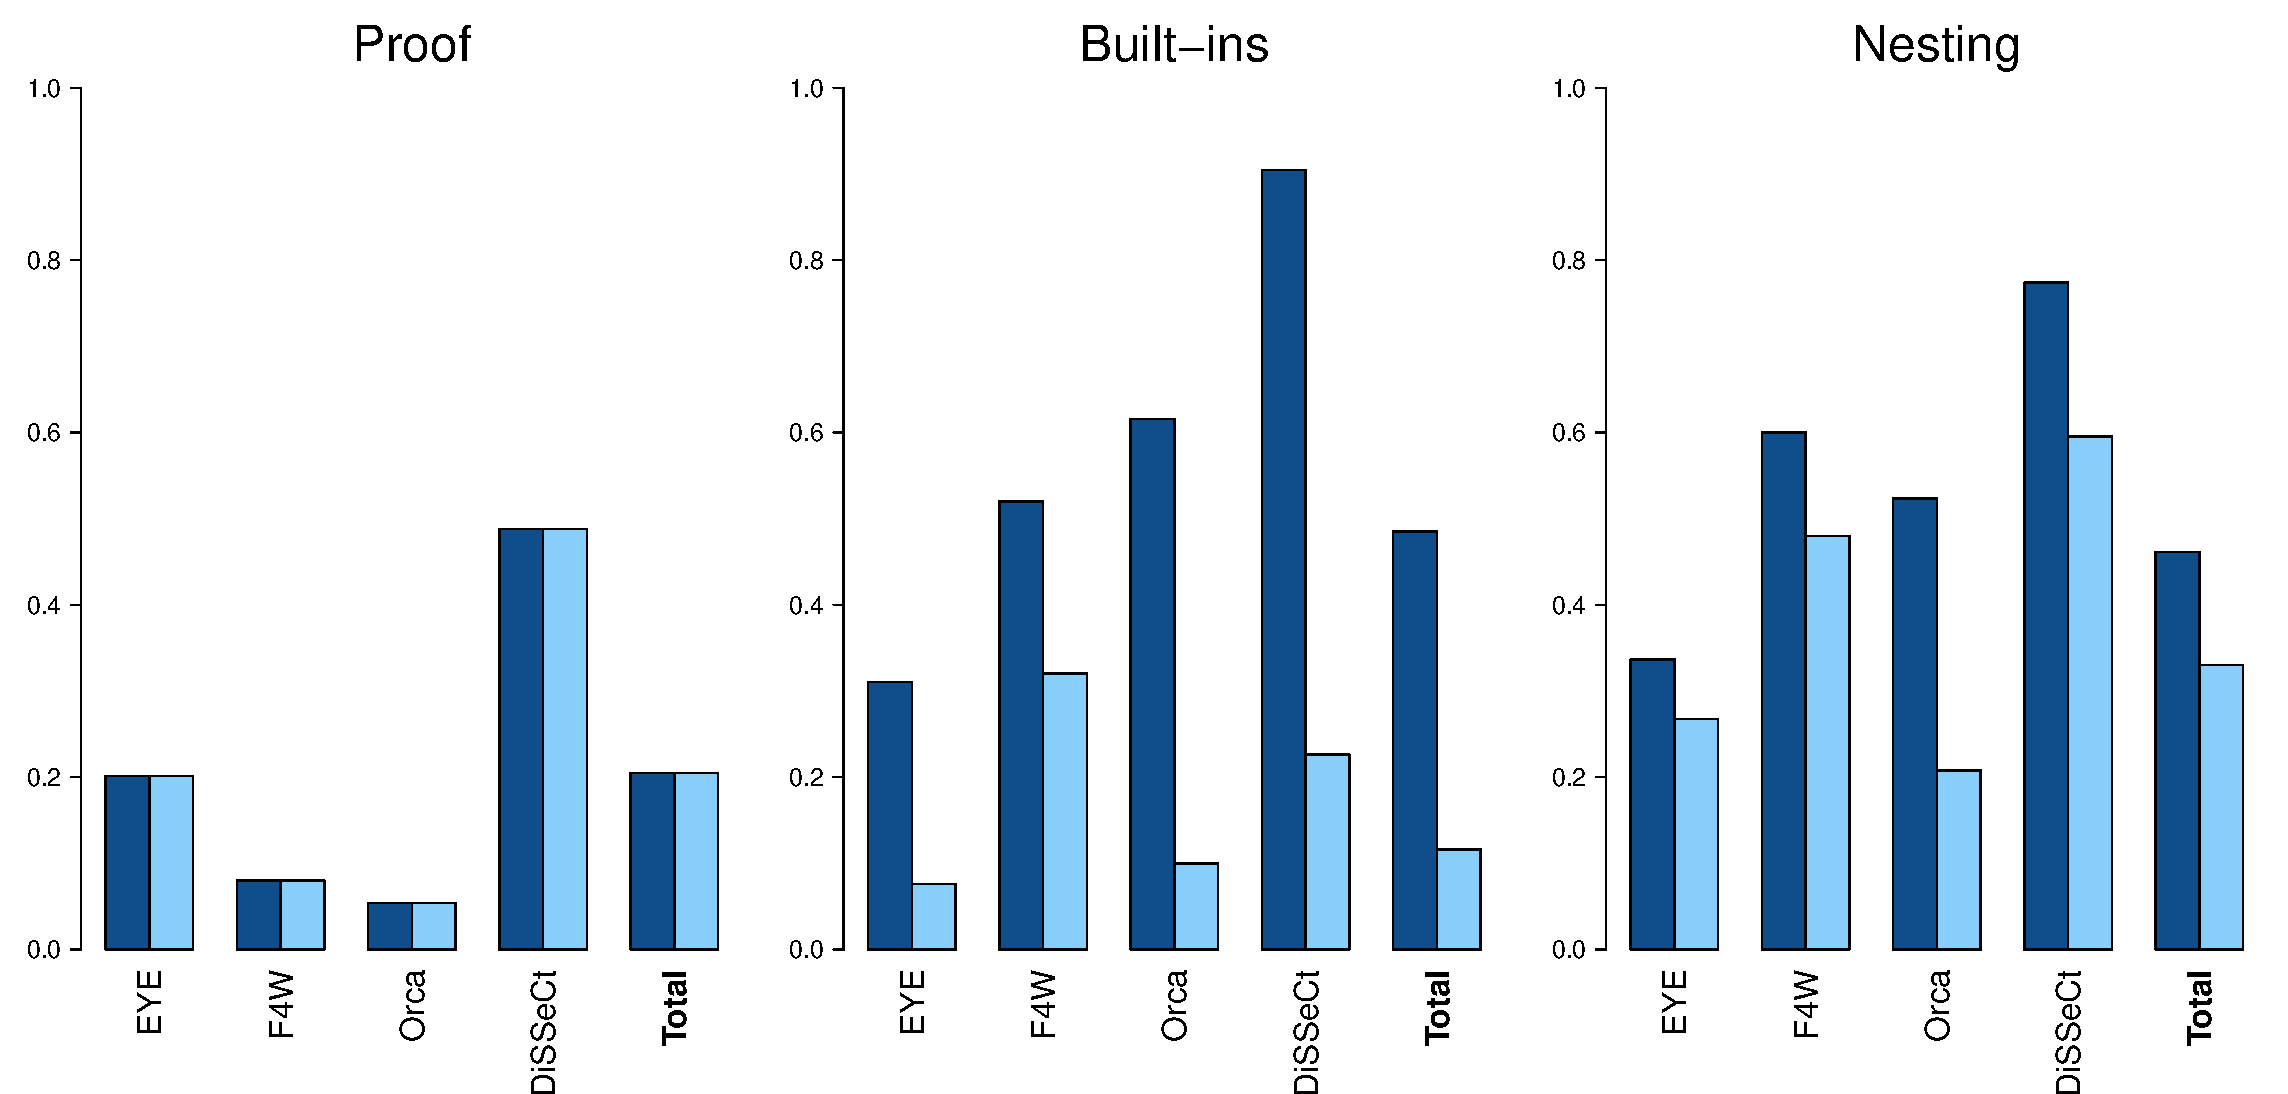
\includegraphics[width=0.95\textwidth]{Rplot06.pdf}
 \caption{Distributions of proofs, built-ins and nesting in datasets. The share in dark blue always represents the files containing the respective feature while light blue is used to represent the cases
 where the feature leads to different interpretations.\label{datasets}}
% \rv{I think this graph can still improve.
%   First, the light blue does not add any information;
%   remove it, so the focus is on the actual information
%   (which makes the figure much more intuitive,
%   as we don't need to read the caption anymore now).
%   Second, consider a different color for the total column.}
% \rv{Can we add extra information,
%   namely the number of cases where there are interpretation differences?
%   So Proofs/EYE now shows 20\%,
%   can we split this into two stacked bars
%   where one is green (no diffs) and one is red (diffs)?}
\end{figure*}

As mentioned above all proof files containing universals and rules cause disagreements which also explains why for the DiSSeCt data set
which consists by 50\% of proofs 60\% of the files are subject to having diverging interpretations. 
The share of built-ins causing differences is rather small, for nesting, which includes the cases of proofs and built-ins, it is rather high. 
Below, we discuss the last two cases in detail. 

%Since almost half of the DiSSeCt data set consists of proofs, it is not surprising that here we also found the highest number of disagreements (60\%).
% Considering Figure~\ref{datasets} it is not surprising that for the DiSSeCt dataset we found the highest share of disagreement between interpretations (60\%):  
% almost half of the dataset consists of proofs. 
% These cause different interpretations whenever rules and universals are involved. 
% The DiSSeCt dataset additionally 
% contains a very high number of built-ins which 
% are often another source of disagreement. 

%  The figure additionally contains the shares of these files where the observed feature (ie proofs, built-ins or nesting) causes problems (light blue). 


\subsubsection*{Disagreements per Formula Type}
To understand how many of the built-ins present in our datasets are causing problems, 
we extended the attribute grammar by additional attributes which test for every built-in whether its subject or its object contains a universal 
variable which -- according to Cwm's interpretation -- is not 
quantified on the $\text{parent}_c$ level of the built in or any higher level. The definition of these attributes can be found in~\ref{cbi}.
 The results of our tests are displayed in Figure~\ref{builtins}. For each dataset we show the percentage of files containing 
at least one built-in construct 
which the two reasoners interpret differently compared to all files containing built-ins. We see that for the whole dataset and most subsets approximately a quarter of all 
files with built-ins contains at least one critical construct. Only in the Facts4Workers dataset this share is higher which can be explained by
the fact that here the built-in \texttt{e:whenGround}\footnote{See \url{http://eulersharp.sourceforge.net/2003/03swap/log-rules.html\#whenGround}. }
 is used in many rules to test whether graph patterns are ground.

 
Similarly to the case just seen, we can ask how many files  of our set of formulas containing nesting have different interpretations caused by deeply nested variables. Since all problems we consider 
in Table~\ref{result} are caused by different interpretations of nested variables -- as this is how we constructed our tests -- we used these numbers to generate Figure~\ref{onlynests}. 
% Here we see how many
% of the files including nesting have conflicting interpretations. 
We observe that, when deep nesting is already present in a file, we suffer from conflicting interpretations in 72\% of the cases.
This is not very surprising since most nested graphs occur in rules which most likely also contain universals, but this figure shows once again, that when using nested graphs, users need to be careful 
with universal variables.

\subsubsection*{Categorisation of Errors}
As a last point in this subsection we categorise the problems observed so far in disjoint groups. 
The reasons for conflicting interpretations of a formula 
can be overlapping. 
% Especially if we have a proof it can be useful to know whether conflicting interpretations are only 
% caused by the proof vocabulary which normally uses graphs -- 
% these cases are rather harmless -- or if built-ins with deeply nested universals in their
% subject or object, or another occurrence of deeper nested universals are involved. 
% a universal variable To test how deeply nested in the formula 
% the deepest nested variable occurs we defined other attributes which we discuss in~\ref{nested}. 
% We measure the depth of a universal variable as one plus the number of formula expressions its quantifier is enclosed in when translating the \nthree formula 
% to its core logic translation according
% to Cwm. If a variable does not occur in a file at all, it has depth 0. Looking back to the formulas we have already seen, we can for 
% example say that in Formula~\ref{fff} the variable \texttt{?y} has depth 2 while \texttt{?x} has depth 1. 
% To calculate the maximum depth of a quantifier in a formula 
% we used attributes. 
% The definition of these can be found in~\ref{nested}.
% 
% Because of the nature of the proof we know that if the maximum depth of the universal quantifiers is two or lower, then the only reason for conflicting interpretations 
% is the use of the 
% predicate \texttt{r:gives} which has a graph as object. If the maximum depth of universal variables is bigger than two, 
% we know that the conflict 
%  found in the proof is more serious and caused by a deeper nesting in one of the formulas occurring in the object of \texttt{r:gives}. 
%
We separate them as follows: 
\begin{description}
\item[Built-in Class] Every formula containing built-in functions used in connection with formula 
expressions containing universals
is counted as such even if this construct occurs in a proof or additionally contains nested graph constructs without built-ins.
\item[Proof Class]
Every proof formula not belonging to the \emph{Built-in Class}
for which the results of all proof steps 
do not contain nested graphs with universal variables which Cwm quantifies on that level are counted as a proof.
\item[Nesting Class]
Every formula not belonging to the two classes above is counted as a nested formula.
\end{description}

To test whether conflicting interpretations are caused by built-ins, we used the attributes introduced above. 
% For the \emph{Proof Class} we needed to determine whether the only reason 
% for conflicting interpretations is the nature of the  proof structure -- in which case the formula is member of the \emph{Proof Class} -- 
% or whether there are universal variables which Cwm quantifies on a deeper level
% than the level of the formula expression cited by \texttt{r:gives} -- these formulas are captured in the \emph{Nesting Class}. 
The method to determine whether a formula representing a proof belongs to the \emph{Nesting Class} or the \emph{Proof Class}  is discussed in~\ref{nested}. 

\begin{figure}
 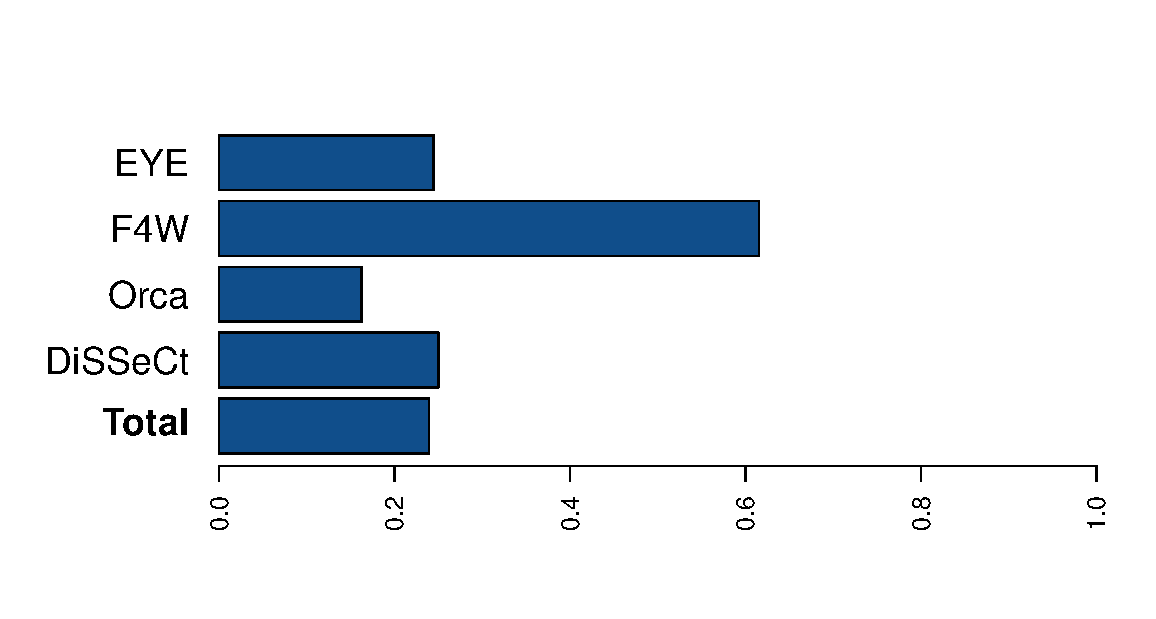
\includegraphics[width=0.49\textwidth]{Rplot10.pdf}
 \caption{Share of files containing built-ins causing conflicting interpretations in
 files containing built-ins. Only in a quarter of all files containing built-ins 
 these occur with deeply nested universals.
\label{builtins}}
\end{figure} 
\begin{figure}
 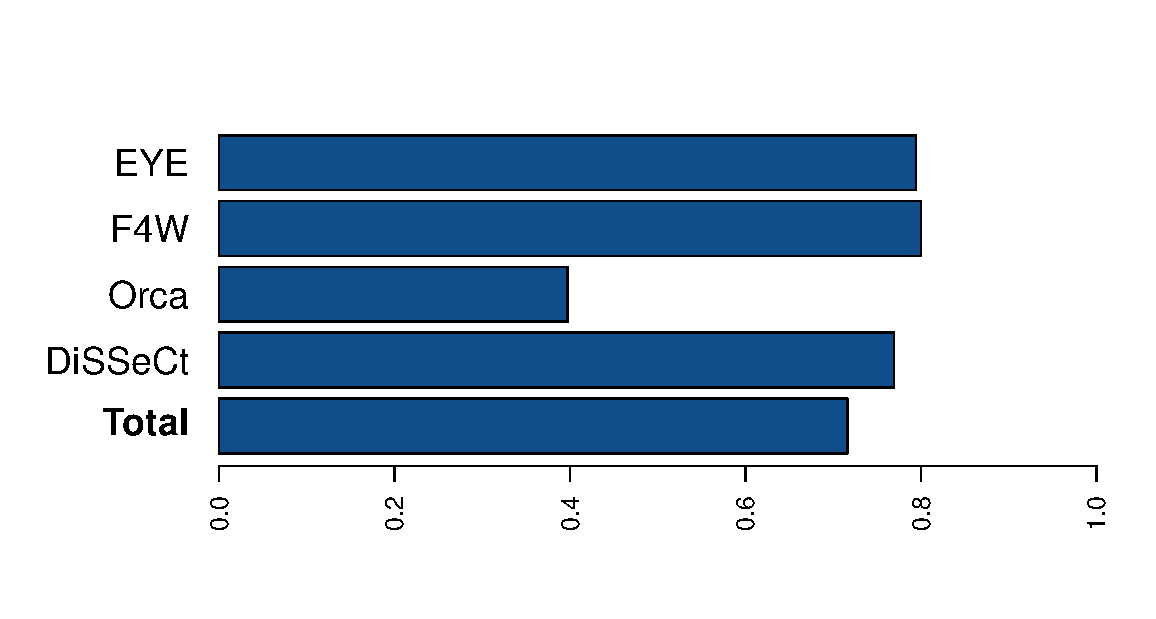
\includegraphics[width=0.49\textwidth]{Rplot12.pdf}
 \caption{Share of files causing conflicting interpretations in
 files which have nested expressions. 72\% of the files containing nesting are interpreted differently by both reasoners.
\label{onlynests}}
\end{figure}

% 
% How are these
% cases distributed within the datasets? 
% To find the different cases we have added two features to our implementation: for every formula parsed, there are evaluation functions providing a number indicating 
% for Cwm's interpretations, how deep the most deeply nested universal quantifiers occur and which variables are quantified under these deeply nested quantifiers.
% If universal quantifiers only occur on top level, the \emph{depth} is one, if a
% universal quantifier occurs in a formula expression which is a direct component of the overall formula, the depth is two, this is for example the case 
% for the formula in Listing~\ref{F4Wcwm}, if a universal quantifier occurs in a formula expression which is component of another formula expression which is a direct component 
% of the overall formula, the depth is three, etc.
% %We do this kind of assignment to determine whether a the formula expressions of a proof contain nested constructions or only rather simple rules as in the example above.
% %
% This assignment enables the above mentioned classification: if a proof has depth two, we know that the proof steps do not lead to formulas with a depth higher than one. 
% If the depth is more than two, we can look up the variables nested more deeply to decide whether they are used in connection with built-in functions or not.


Following this classification, the results of our tests are displayed in Figure~\ref{result2}.
For the overall dataset (last line) half (51\%) of the conflicts between reasoning results occur only because of the different interpretations of proofs. 
As discussed these can be considered as rather harmless. % since they these universal variables normally occur in connection with \texttt{r:gives}.
The next bigger group of differences occurs in connections with built-in functions (31\%). 
Here, not all, but some of the conflicts are unavoidable,
since some built-in functions are not supported by all reasoners. The last group of conflicts (13\%), caused by the simple use of nested graphs or rules 
without direct involvement of built-in functions or proof predicates,  is the most dangerous: while users employing built-in functions are often
aware that the support of these could be limited to one reasoner and therefore also check carefully when they want to switch to a different one, 
this is not the case here. If nested rules and graphs are used without
any special predicates, it is normally expected that the reasoning results from formulas containing these constructions do not differ between reasoners. 
%with these files should be independent of the reasoner. 
The user  has no reason to do extra compatibility checks.

Whether these cases occur depends on the use case: 
In the DiSSeCt dataset, such cases do not occur. This has to do with the fact that the use case here is the test for constraints on \rdf data, ie data 
without formula expressions 
or rules. 
The constraints themselves and the results
are plain \rdf and there is always only one reasoning run applied in order to find constraint violations. In contrast, the Facts4Workers dataset contains
many constructs similar to the one displayed in Listing~\ref{F4W} and does therefore have a rather high occurrence of cases belonging to the last category (33\%).

\begin{figure}
 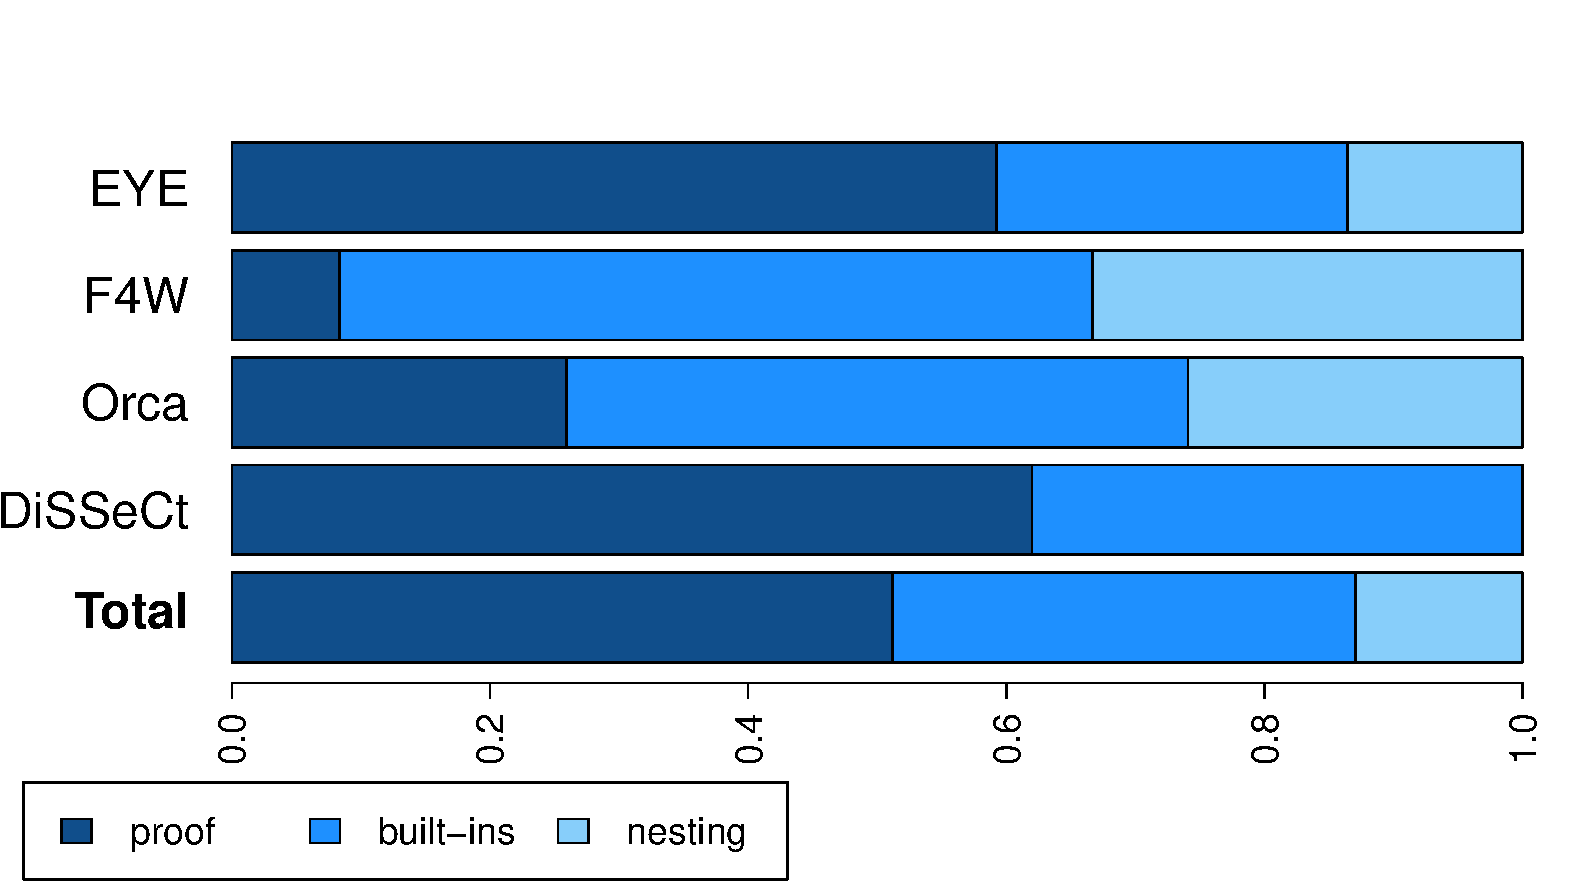
\includegraphics[width=0.49\textwidth]{Rplot14.pdf}
 \caption{Distribution of different cases causing conflicting interpretations by the reasoners Cwm and EYE.\label{result2}}
\end{figure}
% \begin{figure}
% \begin{center}
% \begin{tabular}{lccccccc}
% Dataset & \# of  & \multicolumn{6}{c}{reasons} \\
%         & diff               & \multicolumn{2}{c}{proof}&\multicolumn{2}{c}{built-ins}&\multicolumn{2}{c}{nested graphs}\\
%         &                & \# & \% & \# & \% & \# & \% \\
% \hline
%  EYE  &81 &  48 & 59\% & 22 & 27\%& 11& 14\%\\
%  F4W  &12 &  1 & 8\%& 7 & 58\%& 4& 33\% \\
%  ORCA  &27 & 7 & 26\%&13 & 48\% & 7& 26\% \\
%  DiSSeCt &50& 31 & 62\%&19& 38\%&-&-  \\
%  \hline
% \end{tabular}
% \end{center}
% \caption{Distribution of difference classes per dataset.\label{res2}}
% \end{figure}
% 
% \begin{figure}
% \begin{center}
% \begin{tabular}{lC{1.5cm}C{1.5cm}C{1.5cm}}
% \hline\hline
% Dataset &  \multicolumn{3}{c}{Occurence of reasons for conflicts (in \%)} \\
%         &proof&built-ins&nested graphs\\
% \hline
%  EYE  &  59& 27&  14\\
%  F4W  &   8& 58&  33 \\
%  ORCA  &  26& 48 &  26 \\
%  DiSSeCt & 62& 38&-  \\
%  \hline
%  All & 51&36 &13\\
%  \hline \hline
% \end{tabular}
% \end{center}
% \caption{Distribution of different cases causing conflicting interpretations by the reasoners Cwm and EYE.\label{res2}}
% \end{figure}

\section{Possible solutions}\label{solution}
In the previous section we examined the impact of having different interpretations for nested implicit universal quantification on practical cases and discovered that 31\% of our test files
contained at least one critical construct. This means that the problem is not only of theoretical nature and needs to be addressed. In this section, we discuss possible solutions from two perspectives:
First, we
take the perspective of a
practitioner who -- given the current situation -- needs to make sure that his rules lead to the same result in both reasoners.
Secondly, we take a  broader perspective and clarify
the different positions a standardisation could take.


% and discovered that 
% universal variables are used in nested constructs%such constructs are actually used and sometimes lead to contradictory reasoning results. 
\subsection{Avoiding Conflicts in Practical Cases}
Having seen which kinds of constructs lead to conflicts between the different interpretations of \nthree %and how often they occur in practice,
we now discuss how to deal with those conflicts. One option is to avoid them from the very beginning by not using nested formula expressions. 
The drawback of this solution is that
this also means to not use the full power of \nthree since constructs such as rule-producing rules~\cite{ORCA2} would not be available any more. 
If we want to support \nthree as it is, we need a way to translate from one reasoner to the other.

\subsubsection{EYE formulas interpreted by Cwm}
In order to make \nthree formulas written for the reasoner EYE 
be interpreted in the exact same  way by Cwm, we can use a simple trick: Since we know that the interpretation of implicitly universally quantified variables also depends 
on their contexts, ie on their occurrence in the different conjuncts of a formula, we can add a dummy formula which lifts the scope of deeply nested variables to the top level without changing EYE's interpretation 
of the whole expression.
%that contains universal variables with the same name as the ones occurring in 
%deeply nested formulas. We 
To illustrate that idea we use an example we have seen earlier: remember that in Cwm's interpretation (Interpretation~\ref{iall}) of Formula~\ref{fff} 
the quantifier for the universal variable \texttt{?y} was 
nested while for EYE it was on top level, ie in front of the overall formula (Interpretation~\ref{fff'}). 
If we now add the implication \texttt{\{?y ?y ?y\}=>\{?y ?y ?y\}.}\ to the formula this difference disappears. The formula
\begin{flalign*}\tag{\ref{fff}a}\label{fffa}
&\texttt{\{?y ?y ?y.\}=>\{?y ?y ?y.\}.} \\
&\texttt{\{\{?x :q ?y.\} => \{?x :r :c.\}.\}}\\
&\hspace{4cm}\texttt{=>\{?x :p :a.\}.}\\
\end{flalign*}
has in both reasoners the same interpretation, namely:
\begin{flalign*}\tag{\ref{fffa}'}\label{fffa'}
 & \forall \texttt{x.}\forall\texttt{y.}\\
 &\texttt{\quad<y y y>}\rightarrow\texttt{<y y y>.}\\ 
 &\texttt{\quad< < x q y>} \rightarrow \texttt{< x r c> >}\rightarrow%\\
  %&\hspace{4cm} 
  \texttt{< x p a>.}
\end{flalign*}
Since the antecedent and the consequent of the added rule are exactly the same, its addition does not change the meaning of the whole formula according to EYE. 
For Cwm, the meaning does
change, the quantifier for \texttt{?y} is lifted to the top level and is no longer nested.

While here, the change of meaning has been performed on purpose -- we wanted the formula to have the same interpretation by both reasoners --
phenomena as the one above can also occur rather randomly: In our datasets there are several rules embedded in a bigger context which make use of nested universals but whose
 interpretation does not differ between Cwm and EYE\footnote{A concrete example is the file \url{https://github.com/josd/fluid/blob/master/n3p/sample.n3} in the eye dataset.}. 
 The reason is that they make use of rather arbitrary variable names such as \texttt{?x} and \texttt{?y} 
which are also used in other conjuncts of the same very long formulas. Having that in mind, users of Cwm who want to use nested implicit universal quantification need to be careful
with the variable names they are using to avoid unwanted changes of scope.

\subsubsection{Cwm formulas interpreted by EYE}
Performing the other direction -- making sure that EYE interprets a formula containing universal variables in nested graphs the same way Cwm does -- is more difficult: 
The only way to do so is to use explicit universal quantification as one can easily see recalling Cwm's interpretation of Formula~\ref{fff}: 
\begin{multline}\tag{\ref{fff}'}
 \forall \texttt{x.}
 \texttt{<} \forall \texttt{y.<x q y>} \rightarrow \texttt{<x r c>{}>}\rightarrow\texttt{<x p a>}
\end{multline}
Here the universal quantifier for \texttt{y} is nested, but EYE interprets all implicitly universally quantified variables as quantified on top level.

%Unfortunately, 
Due to the open issues 
mentioned in Section~\ref{remarkExplicitQuantification}, the current version of EYE does not support nested explicit quantification which makes the desired task impossible.
This was different in earlier versions.%
%To get an interpretation such as Formula~\ref{iall} with EYE an older version of the reasoner needs to be used. 
%\rv{The remark about the old version is not that interesting / might be confusing. I would remove it. Or at least phrase it in such a way that I don't have to \enquote{use} an older version, just that it was different in older versions.}
\footnote{In all versions before EYE-2014-12
 nested explicit quantification is allowed.} 
A possible way to make sure that formulas written for Cwm are understood equally by EYE could be to use such an older version of the reasoner.
Then our implementation can be used to generate the representation of an \nthree formula in core logic according to Cwm's interpretation which we could then translate 
 to explicit quantification
in \nthree. But even when doing that, it cannot be guaranteed that this explicit quantification in \nthree works exactly the same way explicit quantification
in core logic does since a formal specification of the former is missing.
Without a clearly defined explicit quantification in EYE, it is not possible for each nested formula to translate Cwm's interpretation to an \nthree formula 
EYE interprets equally.

\subsection{Definition of a Standard}
As discussed above, in the current situation the user writing rules needs to either know beforehand with which reasoning engine he wants to use his rules, or he needs to apply the strategy discussed 
above of adding dummy rules which lift the quantifier of deeply nested implicitly universally quantified variables to the top level. 
Given that \nthreelogic was created for the Semantic Web where interoperability is a very crucial feature, this situation is not acceptable and  
the community needs to come to an agreement. For such an agreement, we see three options which we discuss below.
\subsubsection{Semantics with Nested Universal Quantifiers}
One possible solution could be \todo{Remove!!!}, given that Cwm is the reference implementation of the \wwwc team submission,
to use our specification as a semantics for \nthree and strictly follow that
interpretation. 

One problem with that solution is that it is rather difficult to formalise. 
We needed to define an attribute grammar with four attributes to be able to handle Cwm's implicit universal 
quantification. Following the same approach, scoping on top level only required the definition of one attribute. 
%this kind of formalisation could also be done without employing attribute grammars.
Being a direct realisation of this grammar our implementation is equally complex and so far we did not  encounter an easier way 
to implement the scoping as intended by Cwm.
%When implementing this attribute grammar, we faced the same difficulties and
Even the Cwm reasoner itself has difficulties with implicit universal quantification in some cases (see \ref{bugsincwm}).
To the best of our knowledge, there is no other logical framework supporting implicit universal quantification
which interprets this feature the way Cwm does (we also discuss other frameworks supporting implicit quantification in Section~\ref{iq}).
We therefore suspect that the users' intuition about implicit universal quantification could be opposed to the actual meaning. %But even if that is not the case % and a possible user simply 
%looks up the formalisation to know how implicit universal 
%quantification is understood by the \wwwc team submission,
We furthermore see the
the difficulties when formalising the semantics and implementing a parser or reasoner following it as an indication that end users writing \nthree rules 
could also have problems to 
understand and apply the formalisation of implicit universal quantification according to Cwm. %the \wwwc team submission.

All these reasons make us to rather opt against the possibility to handle implicit universal quantification the way Cwm does.


\subsubsection{Semantics with Quantification on Top Level}
Another possible remedy for the problem at hand would be to strictly follow the interpretation
which understands implicitly universally quantified variables as quantified on top level such as
the reasoner EYE does.

One argument to do so is, that this is easier to formalise and also to implement. The attribute we used for the quantification of EYE was rather simple and just passed all implicitly 
universally quantified variables upwards in the syntax tree. A formalisation could also be made without employing attribute grammars by simply using a universal closure for all universal variables.
As assuming the universal closure for variables freely occurring in  formulas is common practice and done in many frameworks like 
for example Prolog~\cite{Prolog} we expect that users writing \nthree rules can easily understand this behaviour and write their rules 
accordingly.

We therefore favour the interpretation putting the quantifier of implicitly universally quantified variables on the top level.

%which means to assume implicit universal variables to always be quantified on top level. 
% An argument to do so would be that other logical frameworks with implicit universal quantification (like Prolog) also follow this approach. Additionally,
% this kind of universal quantification is rather easy to understand and to implement. 

% Of course this solution deviates from Cwm and thereby most likely from how the \wwwc team submission was meant.
% % the
% % most official document about \nthree and 
% Such a change in the intended meaning of a implicit universal quantification would need to be discussed in the community.

\subsubsection{Exclude Implicit Universal Quantification}
The third solution for the problem explained in this paper would be 
to either not allow implicit universal quantification at all or to at least only allow it in non-nested structures such that the scoping of every implicitly universally quantified variable is clearly
defined in both interpretations. Instead, 
explicit quantification could be employed.
%or at least use it in cases where otherwise interpretations could differ. 
The problem here is that, as explained in Section~\ref{remarkExplicitQuantification},
the meaning of explicit quantification is not clearly defined in the \wwwc team submission either. Problems especially arise if explicit universal quantification is used in combination with explicit
existential quantification -- to be consistent with the implicit case universal quantification always dominates existential quantification if both occur on the same level -- and if constants and 
quantified variables are not clearly distinguished. In order at least make this last opportunity an applicable option, these uncertainties need to be clarified. One possible way to do that would be to
extend the attribute grammar discussed in this paper.

% In order to at least provide the opportunity to apply this last solution to the problem at hand, we plan to extend our interpretation of \nthree to also support 
% explicit quantification. By adding this and other features of \nthree currently not covered in our formalisation, we aim to provide one step further towards the full formal understanding 
% of the power but also the limits of this rule-based logic for the Semantic Web.

% \section{A direct semantics for N3}

\subsection{Formalization of quantification}\label{formal}
%When it comes to semantics of \nthree one aspect where the interpretations chosen by the implementers of reasoning engines differ is the understanding 
%of quantified variables. It is not always clear in which cases the variables with the same name actually mean the same and when they have to be interpreted differently.
%We propose a solution for that problem, which is oriented on the implementation of the EYE-reasoner as it was in December 2013. We start with auxiliary definitions:
%\restdesc descriptions are expressed in the Notation3 (\nthree) rule language~\cite{N3Logic,Notation3}.
%We will introduce the \nthree language and its logic,
%focusing on the aspects relevant to our purposes.
After having discussed the characteristics of implicit quantification in Notation3 in the last section, we now formalize our observations. 
Where possible, we will follow the team submission \cite{Notation3} as this is the most official source indicating how the language is meant to be understood.
%As the dominant reference 
%we will use the team submission as this is the most official source available, which specifies how the logic is meant to be interpreted.
%Where both reasoners differ
%we are following cwm as this reasoner seems to be the closest to the actual specification.

To enable us to distinguish between variables occurring directly in a formula and variables only occurring in formula expressions which are dependent of a formula---as 
it is necessary to interpret for example formula (\ref{eq1})---we give the following definition: 




%%%%%%%%%%%%%%%%%%%%%%%%%%%%%%%%%%%%%%%%%%%%%%%%%%%%%%%%%%%%%%%%%%%%%%%%%%%%%%%%%%%%%%%%%%%%%%%%%%%%%%%%%%%%%%%%%%%%%%%%%%%%%%%%%%%%%%%%%
%Semantics
%%%%%%%%%%%%%%%%%%%%%%%%%%%%%%%%%%%%%%%%%%%%%%%%%%%%%%%%%%%%%%%%%%%%%%%%%%%%%%%%%%%%%%%%%%%%%%%%%%%%%%%%%%%%%%%%%%%%%%%%%%%%%%%%%%%%%%%%%




\begin{definition}[Components of a formula]
Let $f\in F$ be a formula and $c: E \rightarrow 2^E$ a~function such that:
\[c(e)=\begin{cases}
  
  c(e_1)\cup\ldots\cup c(e_n) & \text{if }e=\underline{\texttt{(}}e_1 \ldots e_n\underline{\texttt{)}}\text{ is a list,}\\
  \{e\}  & \text{otherwise.}
\end{cases}\]



We define the set $\textit{comp}(f)\subset E$ of components of $f$ as follows:
 \begin{itemize}
  \item If $f$ is an atomic formula of the form $e_1~ e_2~ e_3.$, $\textit{comp}(f)=c(e_1)\cup c(e_2)\cup c(e_3)$.
  \item If $f$ is an implication of the form $t_{1} \verb!=>!~t_{2}.$, then $\textit{comp}(f)=\{t_1, t_2\}$.
  \item If $f$ is a conjunction of the form $f_1 f_2$, then $\textit{comp}(f)=\textit{comp}(f_1)\cup \textit{comp}(f_2)$.
 \end{itemize}
 Likewise, for $n\in \mathbb{N}_{>0}$, we define the components of level $n$ as:
 \begin{flalign*} 
  \textit{comp}^n(f):= &  
  \{e\in E|\exists f_1,\ldots, f_{n-1}\in F: 
   e\in \textit{comp}(f_1)\wedge  \underline{\texttt{\{}}f_1\underline{\texttt{\}}}\in \textit{comp}(f_2)\wedge \ldots\\& \wedge  \underline{\texttt{\{}}f_{n-1}\underline{\texttt{\}}}\in 
  \textit{comp}(f)\} 
\end{flalign*} 
\end{definition}


The definition allows us to distinguish between direct components and 
nested components. As an example take the following \nthree formula:
%\begin{Verbatim}[fontsize=\normalsize] 
\begin{equation}
\label{cit}		\verb!:John :says {:Kurt :knows :Albert.}.! \end{equation}
%\end{Verbatim}
Direct components are \verb!:John!, \verb!:says! and \verb!{:Kurt :knows :Albert.}! while \verb!:Kurt!,  \verb!:knows! and  \verb!:Albert! are nested components of
level two.

%The definition allows us to distinguish between direct components and 
%nested components. We clarify the deepness of a nesting:

For variables, we can now clarify the deepness of a nesting:



\begin{definition}[Nesting level]
Let $f\in F$ be an \nthree formula and $v\in V$ a variable. The nesting level $n_f(v)$ of $v$ in $f$ 
is defined as follows:
\[
n_f(v):= 
\begin{cases} 
\min\{n\in \mathbb{N}|v\in \textit{comp}^n(f)\} & \text{if } v\in \textit{comp}^n(f) \text{ for some } n.\\
0 & \text{otherwise.}    
         \end{cases}
\]
The nesting level of a formula is defined as: $n(f) = \max_{v\in V} (n_f (v))$.
\end{definition}


As an illustration of the definition, consider the following formula:
\[
 f=\verb! _:x :says {_:y :says {_:x :knows ?z.}.}.!
\]
Here we have $n_f(\verb!_:x!)=1$, $n_f(\verb!_:y!)=2$, $n_f(\verb!?z!)=3$ and $n_f(\verb!?v!)=0$, as the latter does not occur in the formula. The nesting level of that formula is 
$n(f)=3$, as the deepest nested variable \verb!?z! has nesting level 3.

%This definition seems to be a little bit counter-intuitive, especially because we count the nesting level starting from the top of the formula and not, as one might expect, recursively from the bottom.
%The reason for this lies in the way nested universal quantifiers are expected to be interpreted: coming form the top formula, we are always interested in the less nested occurrence of a variable and its 
%direct parent formula, the variables with the same name which depend on this formula and are  are nested deeper are not important for the 


%Variables occurring in \nthree formulas are always implicitly quantified (either universally or existentially). 
%For the interpretation it is crucial to clearly define the scope of each variable. 
%Translated to first order logic, the formula 
%\[
%\verb! {{?x :p :a.} => {?x :q :b.}.} => {{?x :r :c.} => {?x :s :d.}.}.! 
%\]
%should be understood as 
%\[
%(\forall x_1: p(x_1,a)\rightarrow q(x_1,b))\rightarrow (\forall x_2: r(x_2,c) \rightarrow s(x_2,d))
%\]
%and \emph{not} as, for example,
%\[\forall x: ((p(x,a)\rightarrow q(x,b))\rightarrow ( r(x,c) \rightarrow s(x,d)))\]
At first glance this definition might seem counter-intuitive as we count the nesting level starting from the top of the formula and not, as one might expect, from the bottom. This has to do with the
intended meaning of implicitly quantified universals. Only the parent formula of an expression containing a universal is important for its interpretation (see formula (\ref{eq2})). 
All subordinated formulas depending on that formula are handled equally regardless of the degree of their dependency (see formula (\ref{nest})).

The different treatment of universal and existential variables in the interpretation of formulas (\ref{nest}) and (\ref{eq2}) also makes it necessary to define two ways to apply a substitution: 
%one which only acts on the component level and one, 
%which replaces also all nested variable by their substitute:

%it indicates which is the lowest depth a variable occurs and not, as one might expect, the most nested occurrence.  


%\noindent
%To reach this goal, we need to take a closer look to the possible applications of substitutions:

\begin{definition}[Substitution]

Let $A$ be an \nthree alphabet %, $S\subset V$ a set of variables 
and $f\in F$ an \nthree formula over $A$. 
\begin{itemize}
 \item A \emph{substitution} is a finite set of pairs of expressions $\{v_1/e_1, \ldots, v_n/e_n\}$ where each $e_i$ is an expression and each $v_i$ 
 a variable such that $v_i\neq e_i$ and 
 $v_i \neq v_j$,
 if $i\neq j$. 
 %We call each mapping $\sigma: S\cap \text{comp}(f) \rightarrow E$
 %a \textit{component substitution} of $f$. 
 \item %The application $f\sigma$ of a component substitution $\sigma$ 
 For a formula $f$ and a substitution $\sigma=\{v_1/e_1, \ldots, v_n/e_n\}$, we obtain the \emph{component application} of $\sigma$ to $f$, $f\sigma^c$, by simultaneously replacing each $v_i$ 
 which occurs as a \emph{direct component} in $f$ by the corresponding expression $e_i$. 
 \item %The application $f\sigma$ of a component substitution $\sigma$ 
 For a formula $f$ and a substitution $\sigma=\{v_1/e_1, \ldots, v_n/e_n\}$, we obtain the \emph{total application} of $\sigma$ to $f$, $f\sigma^t$, by simultaneously replacing each $v_i$ 
 which occurs as a \emph{direct or nested component} in $f$ by the corresponding expression $e_i$. 
 \end{itemize}
%A substitution $\sigma: S \rightarrow E_g$ is called \textit{ground substitution}, a substitution  $\sigma: S\rightarrow V_E$ \textit{existential substitution}.
\end{definition}

As the definition states, component application of a substitution only changes the direct components of a formula. For a substitution $\sigma=\{\verb!?x!/ \verb!:Kurt!\}$ we obtain:
\begin{multline}
(\texttt{?x :says \{?x :knows :Albert.\}.})\sigma^c  =\nonumber \\ (\texttt{ :Kurt :says \{?x :knows :Albert.\}.})\nonumber
\end{multline}
A total application, in contrast, replaces each \emph{occurrence} of a variable in a formula. with the same example as above, by applying $\sigma$ as a total substitution, we get:
\begin{multline}
(\texttt{?x :says \{?x :knows :Albert.\}.})\sigma^t =\\ (\texttt{:Kurt :says \{:Kurt :knows :Albert.\}.})\nonumber
\end{multline}


%For the following definition, we count the components of each level of a formula $f$ from left to right according to their position in $f$.
This enables us to state how the different kinds of variables in a formula should be treated by an interpretation:




\begin{definition}[Replacements]\label{repl}
Let $f\in F$ be an \nthree formula over an alphabet $A$. Let $v\in V_E$ be an existential and $u\in V_U$ a universal variable. 
For each level $i\in \mathbb{N}$, $i>1$, of $f$, we count with the index $j$ the formula expressions $\underline{\texttt{\{}} f_{ij}\underline{\texttt{\}}}\in \text{comp}^{(i-1)}(f)\cap \text{FE}$ according to
their appearance in $f$ from left to right.


%For each expression $e\in E$ of $A$ let
%$\sigma_e:V\rightarrow E$ be the constant map with $\sigma_e(x)=e$ for all $x\in V$.  
\begin{enumerate}
% \item A \emph{replacement} of $v$ is list $(\sigma_i)_{i\in \mathbb{N}}$ of substitutions $\{x/e_i\}$ for $v$.


 \item 
 An \emph{existential replacement} $\rho_v:F\rightarrow F$ of $v$ is a function consisting of single 
 substitutions $ \{v/e_{ij}\}=\sigma_{ij}$ with $i,j\in \mathbb{N}$ %$(\sigma_{ij})_{i,j \in \mathbb{N}}$ 
 which can be applied by simultaneously performing the component applications $f_{ij}\sigma_{ij}^c$ of the substitutions $\sigma_{ij}$ to the formulas $f_{ij}$. 
 %\\
 %Start with $f=f_{11}$ and perform the following steps:
 % \begin{enumerate}
  
 % \item If $n_f(v)=0$, then $\rho_v(f)=f$.
 %   \item If $n_f(v)>0$ perform the component application of substitution $\sigma_{11}$ on $f$ resulting in $f\sigma_{11}^c$  and perform for each level 
    %perform on each 
   %level 
  % $i>1$ for each formula $f_{ij}$ with $\underline{\texttt{\{}} f_{ij} \underline{\texttt{\}}}\in \text{comp}^{i-1}(f)\cap \text{FE}$ 
   %a component application 
    %of the substitution $\sigma_{ij}$.   
  %\end{enumerate}
  %To emphasize the different substitutions of an existential replacement, we sometimes write it as the set of all its substitutions 
  %$\rho = \{\sigma_{e_f}, \sigma_{e_{f_1}}, \ldots \sigma_{e_{f_n}},\sigma_{e_{f_{1_1}}}\ldots \sigma_{e_{f_{1_m}}}\ldots \sigma_{e_{f_{n_1}}}\ldots \sigma_{e_{f_{n_o}}} $
 \item \label{ur} A \emph{universal replacement}  $\mu_u:F\rightarrow F$ of $u$ is a function consisting of 
 single substitutions $\{u/e_{ij}\}=\sigma_{ij}$ with $i,j \in \mathbb{N}$ %$(\sigma_{ij})_{i,j\in \mathbb{N}}$ 
 which can be applied as follows:\\
 Start with $f=f_{11}$ and perform one of the following steps:
 \begin{enumerate}
 
  %\item If $n_f(u)=0$, then $\mu_u(f)=f$.
  \item \label{a} If $n_{f_{ij}}(u)\leq 2$, perform a total application $ f_{ij}\sigma_{ij}^t$. %of $\sigma_{(i+1)j}$ to $f_{ij}$. %Apply the same componenet substitution to all subformulas  
  %$\underline{\texttt{\{}}f_i\underline{\texttt{\}}}\in \textit{comp}(f)$ and all 
  %to all $u$ with $u\in \textit{comp}^n(f)$ for some $n\in \mathbb{N}$.
  \item \label{b} If $n_{f_{ij}}(u)>2$ 
  repeat %the above mentioned 
  %step (a) or (b) 
  this process
  for each $f_{(i+1) k}$\\with  
  $\underline{\texttt{\{}} f_{(i+1)k} \underline{\texttt{\}}}\in \text{comp}(f_{ij})\cap \text{FE}$. % if $n_{f_{ij}}(u)\leq 2$. 
  %whether 
  %each level 
  %$i\in \mathbb{N}$ formula $f_{ij}$ with $\underline{\texttt{\{}} f_{ij} \underline{\texttt{\}}}\in \text{comp}^{i-1}(f)$ if $n_{f_{ij}}(u)\leq 2$ and perform, if this is the case, a total
  %application $f_{ij}\sigma_{ij}^t$ of $\sigma_{ij}$.
  %, apply this procedure for all $f_i$ with $\underline{\texttt{\{}}f_i\underline{\texttt{\}}}\in \textit{comp}(f)$.
 \end{enumerate}

\end{enumerate}
%For both kinds of replacement
%the subformula index $j$ of a formula $f_{ij}$ is counted from left to right depending on its appearance in $f$.\\
If all substitutions $\sigma_{ij}$ are ground substitutions, i.e. $\sigma_{ij}:\{x\}\rightarrow E_g$, we call the respective replacement \emph{ground}. %\\
%If $V_f$ is the set of variables occurring in $f$ we call all replacements which only consist of substitutions of the form 
%$\sigma_{ij} :\{v\}\rightarrow V_E\setminus V_f$, $v\in V_E$ an %\emph{variable renaming}. Analogously we call it 
%\emph{existential renaming}. 
%Analogously we call $\sigma_{ij} :\{u\}\rightarrow V_U\setminus V_f$, $u\in V_U$
%if the range is $V_E\setminus V_f$ and 
%a \emph{universal renaming}.
%in the case that it is $V_U\setminus V_f$.
 \end{definition}


Note that existential and universal replacements are uniquely defined by the set of their substitutions.\\
%Note, that both definitions can be understood as a set of substitutions which can be applied to 
%Both replacements allow different substitutions for the same variable. While in existential replacement a substitution is always only applied 
%to the \emph{components} of one level of a formula, the substituions used within universal replacement change each \emph{occurrence} of a variable in a (part-)formula. 
The definition states that only existential variables occurring as components in the same (sub-)formula should be treated equally. 
This is different for universal variables. 
To understand how nesting level two is of importance, we come back to our previous example, formula (\ref{eq2}):
\begin{small}\[
f=(\verb!{{?x :p :a.} => {?x :q :b.}.} => {{?x :r :c.} => {?x :s :d.}.}.!) 
\]
\end{small}
For this formula the indexing $f_{ij}$ explained at the beginning of the definition is as follows:\\

\noindent
 \begin{tabular}{ p{3cm}    p{3cm}   p{3cm}  p{3cm} }
%\hline
\multicolumn{4}{l}{ $f_{11}=$}\\
\multicolumn{4}{l}{ $(\texttt{\{\{?x :p :a.\} => \{?x :q :b.\}.\} => \{\{?x :r :c.\} => \{?x :s :d.\}.\}.})$}\\
&&&\\
%\hline
\multicolumn{2}{l}{$f_{21} = $} & \multicolumn{2}{l}{$f_{22} = $}\\
\multicolumn{2}{l}{$(\texttt{\{?x :p :a.\} => \{?x :q :b.\}.})$} & \multicolumn{2}{l}{$(\texttt{\{?x :r :c.\} => \{?x :s :d.\}.})$}\\
&&&\\
  $f_{31}= $& $f_{32}=$& $f_{33}= $& $f_{34}= $\\
    $(\verb!?x :p :a.!)$& $(\verb!?x :q :b.!)$& $( \verb!?x :r :c.!)$& $(\verb!?x :s :d.!)$\\
&&&\\
 \end{tabular}



%$f_{11}=(\texttt{\{\{?x :p :a.\} => \{?x :q :b.\}.\} => \{\{?x :r :c.\} => \{?x :s :d.\}.\}.})$

%{$f_{22} = \texttt{\{?x :r :c.\} => \{?x :s :d.\}.\}.$}

%$f_{11} = f$

%$f_{21} = \verb!{?x :p :a.} => {?x :q :b.}.!$, $f_{22} = \verb!{?x :r :c.} => {?x :s :d.}.!$

%$f_{31}= \verb!?x :p :a.!$, $f_{32}=\verb!?x :q :b.!$, $f_{33}= \verb!?x :r :c.!$, $f_{34}= \verb!?x :s :d.!$.

\noindent Suppose we want to apply a universal replacement $\mu= (\sigma_{ij})_{i,j \in \mathbb{N}}$ for \verb!?x!:\\
As $n_f(\verb!?x!)=3>2$, i.e. \ref{b} is fulfilled, we have to consider the subformulas $f_{21}$ and $f_{22}$ separately.\\
%\[f_{21}=(\verb!{?x :p :a.} => {?x :q :b.}.!)\] \hspace{5cm} and \[f_{22}=(\verb!{{?x :r :c.} => {?x :s :d}.}.!)\] separately.
For $f_{21}$ we get $n_{f_{21}}(\verb!?x!)=2$, which means that \ref{a} is fulfilled. We apply the substitution $\sigma_{21}= \{\verb!?x!/e_{21}\}$ totally on $f_{21}$.\\
We do the same for $f_{22}$. As $n_{f_{22}}(\verb!?x!)=2$, thus \ref{a}, we totally apply the substitution $\sigma_{22}= \{\verb!?x!/e_{22}\}$.
As a result we get:
\begin{small}
\[
\mu(f)=(\verb!{{!e_{21}\verb! :p :a.} => {!e_{21}\verb! :q :b.}.} => {{!e_{22} \verb! :r :c.} => {! e_{22}\verb! :s :d.}.}.!) 
\]
\end{small}
%Both substitutions are applied via total applications such that, 
%if the respective variable occurred in sub-formulas, it would be handled the same way as it is as a~component of 
%$f_{21}$ and $f_{22}$. Note that $e_{21}$ and $e_{22}$ can be different. 
By the total application of the substitutions every nested occurrence of the variable is replaced, we do not have to consider the formulas $f_{3j}$ separately.\\ 
Note that $e_{21}$ and $e_{22}$ can be different. 
Our definition only ensures, that, 
if the same variable occurs in direct sibling formulas, it is treated in the same way, just as in interpretation (\ref{eq2}a).



\subsection{Interpretations and models}\label{semn3}
In this section we are going to embed our concept for evaluation of implicit quantified variables into a definition for the semantics of Notation3.

We start be defining an interpretation function:

%We embed our concepts in the definition of interpretation and semantics:

\begin{definition}[Interpretation]
An interpretation $\mathfrak{I}$ of
an alphabet $A$ consists of:
\begin{enumerate}
\item A set $\mathcal{D}$ called the domain of $\mathfrak{I}$.
\item A function $\mathfrak{a}: 
E_g \rightarrow \mathcal{D}$ called the object function.
\item A function $\mathfrak{p}:
\mathcal{D} \rightarrow 2^{\mathcal{D} \times \mathcal{D}}$ called the predicate function.
\end{enumerate}
\end{definition}

Note that in contrast to the classical definition of \rdf-semantics \cite{rdf} our domain does not distinguish between properties (IP) 
and resources (IR). 
The definitions are nevertheless compatible, as we assume $\mathfrak{p}(p)=\emptyset\in 2^{\mathcal{D} \times \mathcal{D}}$
for all resources p which are not properties (i.e. $p \in \text{IR}\setminus \text{IP}$ in the \rdf-sense). 
By extending given \rdf ground interpretation functions to Notation 3 interpretation functions, the meaning of all valid \rdf triples can be kept in Notation3 Logic. %\\
%Note that 
The main necessary extension would be a function which assigns domain values to ground formula expressions. 
This manner of handling formula expressions makes the expressiveness of such quoting of formulas as in example (\ref{cit}) very similar to \rdf reification \cite{rdf}. 
%Evaluation of concepts within a formula expression can be made via rules. 
%By doing so, we don't allow any extra-evaluation of the ground formulas (as for example 
%By handling ground formulas in that way, we don't allow 
%To use the \rdf ground interpretation functions here 
%By only adding one extra interpretation-function which assigns domain values to formula expressions, \rdf interpretation functions could be used here.  
%Thereby any \rdf-interpretation is also expressible as a Notation3 interpretation.
 %So, the interpretation functions 
%Therefore every \rdf triple can also be interpreted in Notation3.
%Notation3 is more tolerant than \rdf in the sense, that it accepts every kind of expression in all positions (subject, predicate or object).\\ 
%Especially in the object position this makes sense, as it enables us to make statements about formulas as in example (\ref{cit}). We consider 
%the oportunity to use a formula expression in the predicate position as rather theoretical, but we wouln't exclude that there may be cases where 
%this could be a useful feature.\\
%REIFICATION


%This flexibility might raises the question, whether it is really necessary to allow a
%If necessary, the predicate position can easily be restricted.




The following definition combines the replacements of variables and the ground interpretation functions:






\begin{definition}[\label{sem_n3}Semantics of \nthree]
Let $\mathfrak{I}=(\mathcal{D},\mathfrak{a,p})$ be an interpretation of $A$.
Let  $f$ be a formula over $A$ which contains at least one variable, $f_1$ and $f_2$ be ground formulas and $c_1,c_2,p \in E$ be ground expressions.
Then the following holds:
\begin{enumerate}
 \item\label{quant} $\mathfrak{I}\models f$ iff for all universal ground replacements $\mu_1,\ldots,\mu_n$ of the universal variables contained in $f$,  there exist some existential ground replacements
 $\rho_1,\ldots,\rho_m$ of the existential variables in $f$, such that 
 \[\mathfrak{I}\models \rho_1\circ\ldots\circ \rho_m \circ \mu_1\circ\ldots\circ\mu_n(f)\]

 \item $\mathfrak{I} \models c_1\, p\, c_2$. iff $(\mathfrak{a}(c_1),\mathfrak{a}(c_2))\in\mathfrak{p}(\mathfrak{a}(p))$.
 \item \label{conj} $\mathfrak{I} \models f_1 f_2$ iff $\mathfrak{I}\models f_1$ and $\mathfrak{I} \models f_2$.
 \item \label{impl1} $\mathfrak{I} \models \verb!{! f_1 \verb!}! \verb!=>! \verb!{! f_2 \verb!}!$. iff $\mathfrak{I} \models f_2$ if $\mathfrak{I} \models f_1$. 
% \item $\mathfrak{I} \models \verb!{ }! \verb!=>! \verb!{! f_2 \verb!}!$. iff $\mathfrak{I} \models f_2$.
% \item  $\mathfrak{I} \models e \,\verb!=>!\, \verb!{ }!$. for all formula expressions $e$.
% \item \label{fal1} $\mathfrak{I} \models \verb!false! \,\verb!=>!\, e $. for all formula expressions $e$.
 
% \item \label {fal2}$\mathfrak{I} \models \verb!{! f_1 \verb!}! \,\verb!=>!\, \verb!false!$. iff $\mathfrak{I} \not\models f_1$.
\end{enumerate} 
\end{definition}

Number \ref{quant} of the definition respects the constraint explained at the beginning of section \ref{quantsec} and illustrated by example (\ref{both}). % that
%prescribed by the \nthree-website \cite{Notation32}, that in a formula the 
%the scope of all universal quantifications is outside the scope of all existentials. 
This constraint is also the reason, 
why we define two separate mappings which ``ground'' the formulas before further valuation is done.

We finally define a model:

\begin{definition}[Model]
Let $\Phi$ be a set of \nthree formulas. We call an interpretation $\mathfrak{I}=(\mathcal{D},\mathfrak{a,p})$ a \textit{model} of $\Phi$ iff $\mathfrak{I}\models f$ for every formula $f\in \Phi$.
\end{definition}
%
%As in first order logic, we can define the notion of logical implication:

%\begin{definition}[Logical implication]\label{log_impl}
%Let $\Phi$ be a set of \nthree formulas  and $\phi$ a formula over the same \nthree alphabet $A$. We say that $\Phi$ (logical) implies 
%$\phi$ ($\Phi \models \phi$) iff every
%model $\mathfrak{I}\models \Phi$ is also a model of $\phi$.
%\end{definition}


%\section{Findings}







%As a consequence, 
%the interpretation of an existential is slightly different than the of a exisitential quantified variable in first order logic, as it alsways requires the existence of a 
%witness 
%The interpretation of \texttt{false}
%as defined in \ref{fal1} and \ref{fal2} is not supported by every \nthree reasoner. %Nevertheless, we include it in our definition to clarify that not every formula posses a model. 
%Our approach follows the semantics of EYE~\cite{eye}.\\


%\section{Implicit Quantification in other Logics}



\label{exsem}
\newpage
This chapter was partly based on the publications:
\vspace{0.3cm}

\bibentry{arndt_jws_2019}

\vspace{0.3cm}

\bibentry{arndt_ruleml_2015}


%\section{Conclusion}\label{sec:concl}
We conclude this paper in two parts: First, we get back to the research questions which we raised in the introduction and 
summarize how they have been addressed in this paper. In a second part we give an outlook to future work and 
discuss open challenges for the formalisation of \nthreelogic.


\subsection{Review of the Research Questions}
We discuss each research question separately:
\begin{enumerate}
 \item[(i)] \emph{How can we formally express the difference between two interpretations of the same \nthree formula?}
 \end{enumerate}
 To express the interpretations of implicitly quantified variables in \nthreelogic, we defined a core logic (Section~\ref{core}). The syntax of this 
 core logic is very close to the syntax of \nthree and -- apart from some differences in the symbols -- only differs from it in the fact 
 that it only supports explicit 
 quantification. That way, it is easy to express at which position an interpretation sets the quantifier when being faced with implicit quantification
 and to compare different interpretations. 
 For the syntax we also provided a semantics which respects the characteristics 
 of \nthree{} -- like the fact that lists need to be treated as \emph{first-class citizens} -- and allows for further refinement of concepts which have
 not been treated in detail in this paper like the interpretation 
of cited formulas and the definition of \nthree's built-in functions.

To connect an \nthree formula to its core logic counterpart, we chose the concept of attribute grammars (Section~\ref{ag}) and can -- using this concept -- formally
define how an interpretation maps \nthree to core logic.
 \begin{enumerate}
 \item[(ii)] \emph{How do existing interpretations of \nthreelogic conceptually differ in their way of handling implicit quantification?}
% \item[(iii)] What are the consequences of this difference in practice?
% \begin{enumerate}
\end{enumerate}
To answer this research question we first explained that universal quantification is closely related to the concept of a \emph{parent formula} 
(Section~\ref{universals}) which is underspecified in the \wwwc team submission. 
We specified attribute grammars for two different interpretations (Section~\ref{n3}): one seeing the top formula as the \emph{parent formula} of all implicitly universally
quantified variables occurring in it regardless of their level of nesting -- this is the interpretation the reasoner EYE applies -- 
one for which this \emph{parent formula} of an implicitly universally quantified variable is not the direct formula either written in curly brackets \{\} 
or being the top formula
containing the variable
but the next higher formula fulfilling these conditions -- this approach is implemented in Cwm.
\begin{enumerate}
 \item[(iii)] \textit{How often does this conceptual difference lead to conflicting interpretations of formulas used in practical applications?}
 \end{enumerate}
To know whether the conceptual difference in the treatment of implicit universal quantification is not only of theoretical nature but does have impact 
on practical cases we implemented the previously defined attribute grammars in Haskell (Section~\ref{imp}). We applied the implementation to different datasets which were written for 
practical applications and discovered that in 31\% of
all our investigated files at least one construct which is understood differently by the different interpretations can be found (Sections~\ref{data} and \ref{results}).
 \begin{enumerate}
 \item[(iv)]\textit{Which kinds of constructs cause these conflicting interpretations in practice and how likely is it that a file containing 
 these constructs is actually 
 subject to the problem?}
% \item How likely is it that a file containing such constructs leads to conflicting interpretations?
% \end{enumerate}
\end{enumerate}
For the answer of this last question, we looked deeper into the datasets and identified three different categories of constructs which
caused conflicting interpretations, namely proofs, built-ins, and deeply nested formulas without the occurrence of proof-constructs or built-ins 
(Section~\ref{results}). For all these constructs we provided examples and discussed whether the differences in the interpretations are problematic which was especially
the case for nested constructs without built-ins which are not part of a proof. 
We then tested if, given one of these constructs is present in a file, how likely it is 
that this file is treated differently by the two different interpretations. While this was always the case if proofs are present, 
disagreements could also be found for a quarter of the cases containing built-ins and for 72\% of the files containing nested constructs of any kind.
As a last step, we divided the files showing differences in the interpretations into disjoint groups depending on the main reason  causing that difference.
We identified that 13\% of our disagreements were caused by simple nesting without built-ins or proof-constructs. These are the cases we consider as most dangerous 
since files are mostly manually written -- opposed to computer generated proofs -- by users which do not have a specific reasoner in mind.
\\

Especially these cases lead us to the conclusion that the problem of having different interpretations for deeply nested implicit universal quantification needs 
to be addressed by a formalised standard. 
In our opinion, this standard should be easy to understand for users and easy to implement which is why we favour to
the interpretation which understands the top formula as the parent for all universals. 
% But 
% also
% for anyone 
%Being easy to understand and implement, we favour 
% Of the possible solutions we favour the option to follow the the interpretation 
% understanding the top formula as the parent for all universals (Section~\ref{solution}).
% A first, but in our opinion very important, step towards such a standard is to
By providing a way to explicitly express 
the differences between existing interpretations as we did by defining the core logic and showing how attribute grammars can be used to map from
\nthree formulas to that logic, we provided tools which ease the discussion.
Having these tools at hand enables anyone involved to clearly define how he understands implicit universal quantification 
and to test where this interpretation differs
from others. We thereby set a step forward towards the standardisation of \nthree.
% and a mapping from \nthree formula t exemplified of Cwm and EYE in this paper. 
% The newly provided framework enables us and any user to identify the concrete cases where interpretations 
% differ in their understanding of a formula and, hopefully, 
% helps to come to an agreement between different implementers.
% Nested constructs occurring in proofs are often rather harmless. Many cases where built-in functions are involved lead 
% to different interpretations due
% to the fact that not all functions are supported by all reasoners such that the problem of differently defined implicit quantification adds 
% not that much extra damage. But we
% also found cases in almost all of our datasets where nested constructs were occurring without being used in a proof or together with built-in functions. This happened in 13\%
% of the files causing contradictory interpretations. Especially these cases need to be avoided. 

\subsection{Open Challenges and Future Directions} 
While this paper shows how the uncertainties about implicit quantification in \nthree can be clarified the are further challenges lying ahead  
which need to be solved in order to standardise \nthreelogic. 

Next to the clarification of the different ways to interpret implicit quantification in \nthree and a study whether the concrete meaning of existing \nthree files 
changes with a change of the 
interpretation applied, the expressivity of formulas using implicit quantification is an important factor when making a choice how this should be handled. 
Understanding the \emph{parent formula} as the top formula and not as a nested formula makes \nthree with only implicit quantification less expressive. 
Whether this limited expressivity is strong enough to support all the tasks \nthree is meant for and how it compares to other standards needs to be carefully studied 
in order to come to an agreement.

The expressivity of implicit quantification becomes less crucial if \nthree, as intended by the \wwwc team submission, also supports explicit quantification. 
Section~\ref{remarkExplicitQuantification} briefly discusses the problems and uncertainties in the current informal specification. The most important factors are
how the exact position of a quantifier should be taken into account (ie does it make sense that universal quantification always dominates existential quantification) 
and whether or not variables should be separated from constants and have for example a designated name space. These topics need to be discussed in the community. 
We plan to use our core logic to formalise the different options which then, hopefully, leads to an agreement.

Another important topic we excluded from this paper is the formalisation of built-in functions. The \wwwc team submission discusses different predicates which
are considered as part of \nthree like the list functions \texttt{rdf:first} and \texttt{rdf:last} which \nthree inherits from \rdf but also, for example, the predicate 
\texttt{log:equalTo} to state ground equality. We designed the core logic in such way that it can be easily extended to support these and other predicates 
and plan to provide this formalisation as future work.

The last, but probably most critical point, which needs to be tackled in order to standardise \nthree is a clear definition how cited formulas need to be handled. The 
need for such constructs but also the difficulties which come with this kind of standardisation can be observed in \rdf: \rdf reification is excluded 
from the definition of \rdf semantics \cite{RDFSemantics} and 
for the TriG syntax to express named graphs, there is a disagreement about its meaning \cite{TriGsemantics}. We plan to base our own
proposal for 
this part of \nthreelogic on KIF~\cite{kif} and ISO Common Logic~\cite{ICL}.

With the definition of an extendible core logic we provided a framework which can and will help us to clarify all properties of \nthreelogic and thereby
leverage this logic to become a standard for the Semantic Web.


% \chapter{Notation3 Logic as an extension of RDF}
% \section{The semantics of RDF}
% \section{Differences between RDF and Notation3 Logic}





\chapter{Querying and ontology reasoning with Notation3 Logic}\label{others}
In the previous chapters we discussed \nthreelogic, its relation to \rdf and the possibilities to fix its formal semantics. % which is not always clear but can -- once the community comes to an agreement -- be formally specified. 
A clearly defined semantics and compatibility with \rdf were only two requirements on a \emph{Unifying Logic} we identified in Section~\ref{req}.
% After this examination of the logic as a system in itself we now 
% look at the context it was designed for, the Semantic Web. We discussed in Section \ref{req} that 
A \emph{Unifying Logic} for the Semantic Web should furthermore
connect the logical building blocks, \ie the blocks of \emph{Querying}, \emph{Ontologies/Taxonomies} and \emph{Rules}, and it should support the layer of \emph{Proofs}. 
The last point -- proofs -- will be discussed in the following chapter. Here, we focus on \nthree's relation to the logical blocks:
Being a rule logic itself \nthreelogic covers the \emph{Rules} block -- we can perform rule-based reasoning with \nthree.
For \emph{Querying} and \emph{Ontologies/Taxonomies} we need to investigate further: To what extend does \nthreelogic support these two blocks? 
Can it solve the same practical problems as the standards SPARQL and OWL-DL listed in the Semantic Web stack? If yes, is the performance comparable?

%to step back and have a look at the bigger picture: Which tasks can we perform by applying Notation3 Logic?
%Or, coming back to our discussion
%  come back 
% to our initial question
% at this logic of \nthreelogic as a possible candidate to become the unifying logic of the Semantic Web:
% Can we use \nthree to perform the tasks of querying and ontology reasoning in the same use cases SPARQL and OWL are typically used for? 
% How is the performance of the \nthree-based solution in these cases?
In order to answer these questions, we consider two practical use cases which both can be solved by applying a combination of ontology reasoning and querying:\begin{enumerate}
\item a semantic nurse-call system, and
\item a system to perform \rdf validation
\end{enumerate}
Both use cases have been previously implemented by either using OWL-DL or \rdf{}S reasoning and SPARQL querying and we aim to solve them by applying \nthree reasoning instead.
Below, we describe the use cases in detail and discuss how \nthree can 
be used to perform the same tasks as the existing implementations. Both sections finish with a comparison between the approaches. We then conclude our findings.

%\section{General Discussion}\label{gen}
\section{Use case 1: A semantic nurse call system}\label{orca}
% This section consists of three parts: first, we present the use case and the challenges related to it, then we explain how the use case can be approached using \nthree reasoning and as a last part 
% we evaluate our implementation against an implementation which has been done earlier where \owl-DL reasoning and SPARQL querying was employed.
Our first use case is a semantic nurse call system in a hospital:
The system is aware of certain details about personnel and patients represented in an OWL-DL ontology.
Such information can include: personal skills of a staff member, staff competences, patient information, special patient needs, and/or the 
personal relationship between staff members and patients. 
Furthermore, there is dynamic information available, for example, the current location of staff members and their status (busy or free). 
When a call is made, the nurse
call system should be able to assign the best staff member to answer that call. The definition of this ``best'' person
varies between hospitals and can be quite complex. 
The system additionally controls different devices. If for example staff members enter a room with a patient, 
a light should be switched on; if they log into the room's terminal, they should have access to the medical lockers in the room. 

\subsection{Technological challenges}
%Our use case is a nurse call system in a hospital.
The event-driven reasoning system for this use case has to fulfill certain requirements.
\begin{description}
\item[scalability] It should cope with data sets ranging from 1000 to 100,000 relevant triples (ie triples necessary to be included for the reasoning to be correct). 
Especially in bigger hospitals the number of staff members and patients and thereby also the amount of available information about those can be quite big. 
It is not always possible to divide this knowledge into smaller independent chunks as this data is normally full of mutual dependencies. 
\item[functional complexity] It should implement deterministic decision trees with varying complexities. The reasons to assign a nurse to 
a certain patient can be as manifold as the data. Previous work has shown that this complexity is not only theoretically possible but also desired by the 
parties interested in such a semantic system~\cite{accioontold}.
\item[configuration] It should support the ability to change these decision trees at configuration time. Different hospitals have different 
requirements and even in one single hospital those requirements 
can easily change due to eg an increase of available information or a simple change in the hospital's organizational concepts or philosophy.
\item[real-time] It should return a response within 5 seconds to any given event. Especially in such a delicate sector as patient care, seconds can make a difference. 
Even though a semantic nurse call system will not typically be employed to assign urgent emergency calls  through complex decision trees, 
a patient should not wait too long till his possibly pressing request is answered.
\end{description}
% The functional complexity requirement together with the configuration constraint motivate 
% the choice of a reasoning system which supports rules as these can be seen as the most natural way to 
% express decision trees. Even though a numerous amount of OWL DL reasoners support at least one rule format, 
% their reasoning is too slow to meet the scalability and the real-time constraint \cite{ORCA}. \todo{that is the paper used for the first part of this section, so remove reference!}
% Therefore, we chose a rule-based solution. 
%Especially the last argument motivates us to solve the described problem using semantic web technologies as they natively fulfill the semantics requirement.
In a first attempt it has been tried to approach this use case using OWL-DL reasoning:
The represented knowledge can be interpreted by OWL-DL reasoners such as for example Pellet \cite{Pellet}. % or HermiT \cite{hermit}.
Complex decision trees can be handled by subsequent SPARQL queries. It is easy to add new queries or to change the order of existing queries 
and to thereby accommodate for the configuration constraint.
But our tests have shown that such systems inherently are not fast and reliable enough to fulfil the scalability and real-time requirements.
For bigger amounts of data or too complex decision trees, the reasoning times of traditional OWL-DL reasoners grow exponentially, which is not scalable.


 
%\subsection{Implementation} 
% To keep the benefits of an OWL-DL based implementation in a scalable and real-time way, we propose a rule-based solution.
% By using OWL 2 RL rules and resolution instead of classical tableaux reasoning, we can significantly decrease reasoning times and still cover a major subset
% of OWL 2. This approach benefits from the high performance of rule based reasoners. 
% Even for bigger datasets the reasoning times are still faster than with the OWL-DL based approach. %very fast, as we will see later in this paper.  %and is able to reason very fast even over large datasets. 
% %Because of its high performance (see benchmarks mentioned in \cite{eyepaper}), we chose the EYE reasoner for our purposes. As the reasoner is 
% %able to cope with large datasets, our approach meets 
% Also, complex decision trees can directly be implemented in rules. %, as those form the most natural 
% As rules are the most natural representations of such trees, 
% it is easy for a user to understand and change certain priorities 
% or to configure new rules. A further advantage of our approach is that all logic is represented in one single way. Instead of
% OWL plus SPARQL, we can implement the business case by only employing Notation3 Logic (N3). With the aforementioned system, we can meet all necessary requirements.
%We use OWL 2 RL rules to reason about the ontology
% -- syntactically represented Turtle and therefore compatible with \nthree{} -- and add custom rules do model the decision tree. 
% Below, we explain our solution in detail.

\subsection{Ontology reasoning and querying}
Given the shortcomings of the solution using OWL-DL reasoning and SPARQL it makes sense to implement the solution following another approach. 
Below, we describe how we used \nthreelogic to solve the problem.

\subsubsection{OWL RL in \nthree}\label{owlrln3}
If we use a traditional OWL DL reasoner like for example Pellet \cite{Pellet} or HermiT \cite{hermit} to reason over an existing ontology 
this reasoner 
natively understands the concepts which are part of the OWL DL profile and applies 
different inference steps in a predefined order to derive new knowledge. % applying a tableaux algorithm (see for example \cite[chapter 2]{dl}).
%  
% 
% 
% Every \owl ontology has a representation in \rdf/XML (see also Section~\ref{rdfandowl}). This can easily be translated to \rdf/Turtle which then is syntactically compatible with 
% \nthree. 
% 
% 
% 
% % General explanation: ABox, TBox. representation of the knowledge against reasoning.
% % 
% % Say  that N3 is interesting because we can make rule-producing rules.
% % 
% % 
% Traditionally, reasoning over OWL ontologies was performed by description logic based reasoners using (variants of) the tableaux algorithm.
% Prominent examples of such reasoners are Pellet \cite{Pellet} and HermiT \cite{hermit}. 
% Both support---as others of their kind---the full OWL DL profile. 
%As the OWL-DL profile is very expressive and contains a huge variety of different concepts and the complexity of the related reasoning,
As OWL DL is very expressive and contains a huge variety of different concepts, OWL DL reasoners perform rather slow in comparison with, for example, rule-based reasoners. 
% which mostly only
% apply one kind of inference step.
The OWL 2 profiles \cite{OWLRL} aim to overcome this gap 
by defining less expressive
but still powerful subsets of OWL DL. One of these profiles is OWL RL, which was designed to enable rule-based reasoners to cope with OWL ontologies. 

For each OWL concept which forms part of the RL profile the specification lists one or more rule %which can be written in a rule language with at least the expressiveness of Datalog~\cite{datalog}
which can be used to draw conclusions from it. These rules written in a generic \rdf rule language with the expressiveness of Datalog~\cite{datalog} -- ie simple rules which do not allow functions 
or new existential variables in their conclusion
-- and can be translated to 
every rule language being at least equally expressive. 
These rules then either directly act on the syntactical representation of the ontology -- this is what we do in our implementation -- 
or on its translation to the input format of the rule language -- this is for example done by OWLim \cite{owlim} and Oracle's RDF Semantic Graph \cite{oracle}.
%The advantage of specifying rules in a format which is compatible with \rdf and reason directly on the ontology is that it remains transparent which rules are used and 
By using \nthree which is compatible with \rdf/Turtle we make sure that the reasoning performed does not depend on the way the triples are translated to an internal format. 
In that sense we are reasoner independent. This approach furthermore makes it easier for the data consumer to understand or choose which rules are applied.  
% 
% if that is not \rdf.
% %and have been translated and used in different formats and by different reasoners like 
% %as for example the reasoners 
% An example for the latter are the reasoners OWLim \cite{owlim} and Oracle's RDF Semantic Graph \cite{oracle} which both use an internal rule-language 
% for reasoning not directly related to \rdf.
% %  In these last two reasoners, as well as most other reasoners we are aware of, the rules are 
% %  written and stored in an internal rule format which makes it difficult for the user to understand the derivations made or to choose which concepts should be supported by a a reasoner in a 
% %  specific use case.
% %Of course these rule language needs to act on the specific 
% As a consequence the 
 
% In our implementation we use \nthree rules: As the \rdf representation Turtle is fully compatible with \nthree, the syntactic representation of the ontology can directly serve as input 
% for the reasoner. The rules can be written in the same language and thus be exchanged between different reasoners. 
%
% The idea here is that the \rdf representation of the ontology serves as input for the reasoner and the derivations which can be made based on the semantics of the different 
% OWL concepts are supported by rules. These rules need  to be specified in the rule language. % and the website
%We started from an OWL-DL ontology which was used to 
%Possible data which can be processed by our system  
%The ACCIO Ontology
% 
% To be able to support OWL 2 RL reasoning in N3 we used the OWL 2 RL/\rdf rules as listed on the corresponding website~\cite{OWLRL}. 
% Where possible, we made use of existing N3-translations of these rules as provided by EYE~\cite{EYEowl}. 
% Missing concepts were added. 
% The knowledge about patients, staff and the hospital set-up in general was specified using the ACCIO  ontology\footnote{Available at: \url{https://github.com/IBCNServices/
% Accio-Ontology/tree/gh-pages}}\cite{accioont}.
% Even though this ontology is designed for OWL-DL reasoning, the limitation to OWL RL had no impact for 
% our specific use case. %, all derivations needed to cope with the desired decision trees were supported by OWL RL. 
% 
% 
\begin{lstlisting}[
  float=t,
  caption={OWL-RL rule for \texttt{rdfs:subClassOf} class axiom in N3.},
  label=lst:subclass]
§\textcolor{gray}{@prefix rdfs: <http://www.w3.org/2000/01/rdf-schema\#>.}§
§\textcolor{gray}{@prefix rdf: <http://www.w3.org/1999/02/22-rdf-syntax-ns\#>.}§

{?C rdfs:subClassOf ?D. ?X a ?C} => {?X a ?D}.
\end{lstlisting}
% To illustrate the idea of using rules for OWL reasoning, we give a small example: Listing~\ref{lst:subclass} shows 
% the class axiom rule\footnote{The rule is the N3 version of the cax-sco rule in Table 7 on the OWL 2 Profiles website~\cite{OWLRL}.} which is needed 
% to deal with the rdfs concept
%  \verb!subclassOf!. For convenience we omit the prefixes in the formulas below. The empty prefix refers to the ACCIO ontology, 
%  \verb!rdf! and \verb!rdfs! have the same meaning as in Listing~\ref{lst:subclass}. Consider that we have the following T-Box triple stating that the class \verb!:Call!
%  is 
%  a subclass of the class \verb!:Task!:
%  %If the ontology contains the triples
% \begin{equation}
%  \verb!:Call rdfs:subClassOf :Task.! \label{1}
% \end{equation}
% If the A-Box contains an individual which is member of the class \verb!:Call!
% \begin{equation}\verb! :call1 a :Call.! \label{2}\end{equation}
% %a rule based reasoner can use the rule given in listing \ref{lst:subclass} to conclude 
% an OWL DL reasoner would make the conclusion that the individual also belongs to the class \verb!Task! 
% \begin{equation}
%  \verb!:call1 a :Task.! \label{3}
% \end{equation}
% Our rule in Listing \ref{lst:subclass} does exactly the same: as Formula~\ref{1} and Formula~\ref{2} can be unified with the antecedence of the rule, a reasoner derives
% the triple in Formula~\ref{3}. Other concepts can be handled similarly.
% 
%In a first attempt to solve the above-mentioned problem we used a direct translation of 
% How this can be done is explained in the specification of OWL RL~\cite{OWLRL} where the concrete OWL 2 RL/\rdf rules
% are listed in a generic rule language. %as listed on the corresponding website. 
% 
% As \nthree is compatible with Turtle -- one representation format of \rdf -- 
%
%Where possible, we made use of existing N3-translations of these rules as provided by 

Below, we explain OWL RL reasoning in \nthree on a concrete example taken from our use case.
The OWL RL rule we show as well as the other used in our implementation are taken from the EYE website~\cite{EYEowl}. %, where needed, additional rules were added following the 
Knowledge is represented using the ACCIO ontology \cite{accioont} which will be further described in section \ref{ont}.
% The results of this 
% implementation were already promising \cite{arndt_ruleml_2015},\todo{replace reference} but for larger data sets the reasoning took multiple minutes and, thus, did not meet the requirements claimed above. 
% We explain the idea behind these OWL RL rules in \nthree %and how they can be improved
% using
% %We start with 
% an example:
Listing~\ref{lst:subclass} shows 
the class axiom rule\footnote{The rule is the N3 version of the cax-sco rule in Table 7 on the OWL 2 Profiles website~\cite{OWLRL}.} which is needed 
to deal with the \rdf{}s concept  \verb!subclassOf!.
For convenience we omit the prefixes in the formulas below. The empty prefix refers to the ACCIO ontology, 
 \verb!rdf! and \verb!rdfs! have the same meaning as in Listing~\ref{lst:subclass}. Consider that we have the following %TBox 
 triple stating that the class \verb!:Call!
 is 
 a subclass of the class \verb!:Task!:
\begin{equation}
 \verb!:Call rdfs:subClassOf :Task.! \label{1}
\end{equation}
If the ontology %ABox 
contains an individual which is member of the class \verb!:Call!
\begin{equation} \verb! :call1 a :Call.! \label{2}\end{equation}
an OWL DL reasoner would make the conclusion that the individual also belongs to the class \verb!Task!: 
\begin{equation}
 \verb!:call1 a :Task.! \label{3}
\end{equation}
Our rule in Listing \ref{lst:subclass} does exactly the same: as Formula~\ref{1} and Formula~\ref{2} can be unified with the antecedent of the rule, a reasoner derives
Formula~\ref{3}. 
%


\subsubsection{Decision trees}
%REMARK: Still not sure whether we need this section?
%The decision trees which have to be implement
%As mentioned above, decision trees as needed in for real life use cases can be quite complex. 

%Depending on the amount of available information, decision trees for nurse call systems can be quite complex. The ACCIO ontology 
%supports a huge variety of different concepts. %It is possible to model the profile of a patient (among others the 
 
The ACCIO ontology provides the user with a huge variety of concepts which can, eg be used to describe patients (social background, needs, disease), 
staff members (skills, relationships to patients), and situations (locations of persons, states of devices). If all this information is actually available, decision trees
can use all of it and be therefore quite complex. Here, we provide two simple rules which could be part of such a tree and we explain how these rules can
be modified depending on the needs of an individual hospital.
 
 \begin{lstlisting}[
  float=t,
  caption={Rule assigning a preference value to a staff member with status "free" who is close to the call-location. },
  label=lst:ex]
§\textcolor{gray}{@prefix : <http://ontology/Accio.owl\#>.}§
§\textcolor{gray}{@prefix rdf: <http://www.w3.org/1999/02/22-rdf-syntax-ns\#>.}§

{
  ?c rdf:type :Call.
  ?c :hasStatus :Active. 
  ?c :madeAtLocation ?loc. 
  ?p :hasRole [rdf:type :StaffMember].
  ?p :hasStatus :Free.
  ?p :closeTo ?loc.
}
=>
{
  (?p ?c) :assigned 200.
}.
\end{lstlisting}
 
Listing~\ref{lst:ex} shows a rule which, given an active call, assigns a staff member with a certain preference to that call. 
As explained in Section~\ref{prn3}, \nthree reasoners can be used goal-driven: The reasoner outputs all instances of the result of a filter rule which it can derive 
based on the input at hand, in our example all combinations of persons assigned to calls and their preference number. 
By using built-in functions we can now search for the highest or lowest preference number.
%By using built-in functions, such a filter can find the minimum or maximum values for certain conditions.
% Using built-in functions we can write a query which searches 
% % The EYE reasoner works 
% % with filter rules (queries), 
% %This makes it easy to search
% for the assignment of a staff member with the lowest or highest number. 
In our example, lower numbers mean higher preferences. The antecedence of the given rule contains certain constraints: the active call is made on a certain location and
there is a staff member, who is currently free and close to that location. In such a case, our rule assigns the number 200 to the combination of call and staff member.

\begin{lstlisting}[
  float=t,
  caption={Rule assigning a preference value to a busy staff member who has the needed skills to answer the call. },
  label=lst:ex2]
§\textcolor{gray}{@prefix : <http://ontology/Accio.owl\#>.}§
§\textcolor{gray}{@prefix rdf: <http://www.w3.org/1999/02/22-rdf-syntax-ns\#>.}§

{
  ?c rdf:type :Call.
  ?c :hasStatus :Active.
  ?c :hasReason [rdf:type :CareReason].
  ?p rdf:type :Person.
  ?p :hasStatus :Busy.
  ?p :hasRole [rdf:type :StaffMember].
  ?p :hasCompetence [rdf:type :AnswerCareCallCompetence].
}
=>
{
  (?p ?c) :assigned 100.
}.
\end{lstlisting}



Listing~\ref{lst:ex2} displays another rule: here, the reason of the active call is known. We have a staff member who has the required 
skills to answer that kind of calls, but this staff member is currently busy. Our rule assigns the number 100 to this
combination of call and staff member. This means, in our current decision tree, we prefer this assignment to the one described by Listing~\ref{lst:ex}.

Now, it could be, that another hospital has different priorities. Imagine for example that in this new hospital, no busy staff should be called 
if there is still a free staff member available, regardless of the reason of the call. We could easily adapt our decision tree by simply changing the assignment number 
of one of the rules. If we replace the triple \[\verb! (?p ?c) :assigned 100.!\] in line 15 of Listing \ref{lst:ex2} by the triple \[\verb! (?p ?c) :assigned 300.!\]
the reasoner would prefer the assignment expressed by Listings \ref{lst:ex} to~\ref{lst:ex2}.

 
Similarly, we can add extra conditions to the rules. Currently, the rule in listing \ref{lst:ex2} does not take the location of the staff member into account. We can
change that by only adding the triples 
\[ \verb!?c :madeAtLocation ?loc. ?p :closeTo ?loc.!\]
to the antecedence of the rule. To give this new rule a higher priority than the existing one, we would again only have to change the assigned number in the consequence.
Rules with the same number are treated equally.



\subsection{Improving the solution by pre-producing TBox-rules}\label{reasoning}
In a first attempt we implemented the reasoning and querying as explained above and could already perform better than the solution employing \owl reasoning and SPARQL querying. 
However, we could not meet the requirements mentioned above: our reasoning did not scale well and and it did not fulfil the real-time constraint. 
For that reason, we used an optimisation strategy 
which takes advantage of a specific feature of \nthree: 
In \nthree it is possible to write and apply rules having new rules in their consequences, we call these \emph{rule-producing rules}. 

% The key idea of our approach is now that there 
% is some knowledge in the ontology which does not change at execution time of the reasoning system: The fact that a call is a kind of task as specified in Formula~\ref{1} will not be changed 
% by the fact that for example a nurse is moving from one room to another.


% and have been translated and used in different formats and by different reasoners like for example 
%  OWLim \cite{owlim} and Oracle's RDF Semantic Graph \cite{oracle}. In these last two reasoners, as well as most other reasoners we are aware of, the rules are 
%  written and stored in an internal rule format which makes it difficult for the user to understand the derivations made or to choose which concepts should be supported by a a reasoner in a 
%  specific use case.
% Various implementations make use of 
% the OWL 2 RL/\rdf rules as proposed in the specification, among them
%  OWLim \cite{owlim} and Oracle's RDF Semantic Graph \cite{oracle}. 
% As most other implementations we are aware of, these reasoners support their own rule format, 
% and optimizations are done internally using
% the underlying programming language. 
% We propose an optimization which can be done in the logic itself by performing an extra reasoning step.
% We are thereby independent of a specific reasoner.

To better understand how we can benefit from rule-producing rules we go back to the above example: 
By unifying the antecedent of the rule in Listing~\ref{lst:subclass} with Formulas~\ref{1} and \ref{2} we could derive Formula~\ref{3}.
But this unification is rather expensive: The antecedent contains three different variables occurring 
in two different triples which have to be instantiated with the data of the ontology. % and this unification needs to be done whenever a new call is made.
%Our idea is now to make these unifications as early as possible and not
%We use rule-producing rules to do a pre-reasoning step: 
%Our solution now distinguishes between static and dynamic data: 
While information as stated in 
Formula~\ref{2} can change -- patients will make new calls -- statements as Formula~\ref{1} can be considered as fixed.
% and we can thus already perform this part of the unification before 
% we encounter 
The terminology does not change during the reasoning process,
calls are tasks for our ontology. %Our solution makes use of this observation: 
%The ontology contains more triples like Formula~\ref{1} which specify the terminology: % as for example classes and their relationships among each other.
Triples as the above specifying the terminology of an DL ontology are known as the TBox \cite[chapter 1]{dl}. 
%A description logic ontology consists of two parts: the TBox and the ABox \cite[chapter 1]{dl}.
% What is valid for Formula~\ref{1} also counts for 
% the other triples specifying the terminology. 
%In description logic these kinds of triples together form the TBox \cite[chapter 1]{dl}, the terminological knowledge.
Here the broader concepts (classes) and their relationships among each other are specified  
while the ABox contains triples over individuals.
We consider the
TBox as static knowledge which can be used for pre-processing. The idea of our solution is to do as much unification as possible before dealing with (possibly) dynamic data. 
We produce more specialized rules, in the case mentioned above, for example the rule
%
\begin{equation} 
\verb!{?X a :Call.} => {?X a :Task.}.!
\label{4}
\end{equation}
which will derive for every new call, that it is also a task, just as the rule in Listing~\ref{lst:subclass} does.

%Below we describe how we produce specialized rules based on the concepts present in the ontology's TBox, 
%with 
Below we describe our implementation.
% Reasoning in EYE can be considered as a single  process, having as input all necessary files representing the knowledge 
% (ie the necessary ontologies, data, and rule-files), and a query-file that filters the output of the reasoning result.
%We use the EYE reasoner and
We perform two steps:
\begin{enumerate}
 \item Produce a grounded copy of the  TBox. 
 \item Use rules to translate the grounded TBox into specialized rules.
\end{enumerate}

The need of the first step has to do with the fact that 
OWL ontologies represented in \rdf often use \emph{structural blank nodes} (see Section~\ref{strucblanks}):
As for example the union or the intersection of two classes cannot directly serve as subject of object in a triple, an anonymous blank node is normally introduced in such cases to
represent the construct.
% Blank nodes are for example used to represent the anonymous class  
% for concepts as for example intersection or union of classes ontology can contain anonymous classes represented by blank nodes.
Used in rules, 
these blank node class names have a 
limited scope (remember the examples from Section~\ref{existentials}). It is therefore difficult to use them to reference the same class in different rules. 
We will give a more elaborate explanation in the next section. 
After that we will describe the translation step in more detail.



\subsubsection{Grounding the Ontology}
\begin{lstlisting}[
  float=t,
  caption={ACCIO example: a call is both, a patient task and an unplanned task. },
  label=task]
§\textcolor{gray}{@prefix : <http://ontology/Accio.owl\#>.}§
§\textcolor{gray}{@prefix owl: <http://www.w3.org/2002/07/owl\#>.}§
§\textcolor{gray}{@prefix rdf: <http://www.w3.org/1999/02/22-rdf-syntax-ns\#>.}§
§\textcolor{gray}{@prefix rdfs: <http://www.w3.org/2000/01/rdf-schema\#>.}§

:Call  rdfs:subClassOf [ 
                       rdf:type owl:Class ;
                       owl:intersectionOf ( 
                                     :PatientTask
                                     :UnplannedTask
                                   )
                       ].
\end{lstlisting}


Before translating the TBox into rules we have to replace all blank nodes by \uris or literals. To understand the reason for this skolemization step, 
consider Listing~\ref{task}.
The example contains triples which further describe the class \texttt{:Call} from Formula~\ref{2}.
A call is a patient task and an unplanned task, or to be more specific:
There exists an anonymous class of which the class \texttt{:Call} is a subclass and which is the intersection of 
the classes \texttt{:PatientTask} and \texttt{:UnplannedTask}. 
%Even though \nthree supports rules which contain blank nodes,
It is exactly this anonymous class which causes problems. As we discussed in Section~\ref{strucblanks}
blank nodes are not simply variables, they are variables with an implicit existential quantifier and a specific scope. 
If we take the triple
\begin{equation}
 \texttt{:Call rdfs:subClassOf \_:y.}
\end{equation}
from line 6 of Listing~\ref{task}\footnote{Remember that \texttt{[ ]} stands for a ``fresh'' blank node, we chose to name it \texttt{\_:y} to make it easier to refer to it.}
and try to construct a rule from it in an analogous way as we did with Formula~\ref{1} and its resulting Rule~\ref{4} we would most probably come up with something like: 
%Being unlabelled, the blank node can be referred by an arbitrary new blank node name. A translation as done in Formula~\ref{4} would result in a rule like:
\begin{equation}
\verb!{ ?X a :Call. } => { ?X a _:y.}.! 
\label{newblank}
\end{equation}
But here the blank node \texttt{\_:y} is quantified in the consequence of the rule, in \nthree Core Logic this translates to:
\begin{equation}\tag{\ref{newblank}'}
 \forall\texttt{x: <type(x,Call)>}\rightarrow \texttt{<}\exists\texttt{y: type(x,y)>}
\end{equation}
This rule means, that every instance of the class \texttt{:Call} is also instance of \textit{some} other class. 
This knowledge can already be derived from Formula~\ref{4} where we have an example of such a class. 
% 
% and does 
% not have much influence 
% on further reasoning. And even if the blank node in Listing~\ref{task} would be labeled by, for example, \texttt{\_:intersection1} a new rule
% \begin{equation}
% \verb!{ ?X a :Call. } => { ?X a _:intersection1.}.! 
% \label{union}
% \end{equation}
% would have no other meaning than Formula~\ref{4} as in \nthree the scope of a blank node is always only the graph, i.e. the curly brackets \texttt{\{ \}}, 
% in which it occurs  \cite{Notation3, arndt_ruleml_2015}. 
With the local scoping of the blank node in the consequence of the rule, it is impossible to make the connection  between the class mentioned in the rule and the  
%The consequence of the rule would not refer to our 
intersection class of patient tasks and unplanned tasks by using blank nodes. We need to choose a constant representing the intersection class mentioned in Listing~\ref{task} 
which does not not change its scoping when used in the consequence of the rule. 

As \owl ontologies use a lot of such structural blank nodes which here can be understood as anonymous classes, we perform a grounding step.
Our implementation uses the EYE reasoner which provides the option to obtain a skolemized version of any input
\nthree file(s). 
The switch \verb!--no-qvars! replaces every blank node by a unique skolem \iri following the naming convention as described in the \rdf specification \cite{rdf}.
It additionally makes sure that equally named blank nodes only get assigned the same skolem \iri if they actually refer to 
the same thing. Producing a grounded version of the ontology enables us in further reasoning steps to use the 
new identifiers for (formally) anonymous classes in different rules.

\subsubsection{Translation Step}

 \begin{lstlisting}[
  float=t,
  caption={Rule producing new rule for every occurrence of \texttt{rdfs:subClassOf}; based on the \texttt{rdfs:subClassOf} class axiom of Listing~\ref{lst:subclass}.},
  label=lst:subclass2]
§\textcolor{gray}{@prefix rdfs: <http://www.w3.org/2000/01/rdf-schema\#>.}§
§\textcolor{gray}{@prefix rdf: <http://www.w3.org/1999/02/22-rdf-syntax-ns\#>.}§

{?C rdfs:subClassOf ?D.} => {{?X a ?C.}=>{?X a ?D.}.}.
\end{lstlisting}



As explained above, the next step after having produced a grounded version of the ontology's TBox is to produce the new specialized rules. 
Here we use rule-producing rules. %, we make use of a property of Notation3:
%we use rules can not only be applied to derive new triples but also to derive new rules. 
To understand the idea, consider the following example: 
%We explain the 
\begin{multline}\notag
 \texttt{\{}\underbrace{\texttt{:Call rdfs:subClassOf :Task.}}_{\text{\normalsize satisfied ontology triple(s)}} \texttt{\}}\\\texttt{=>\{}\underbrace{\texttt{\{?X a :Call\}=>\{?X a :Task.\}.}}_{\text{\normalsize produced new rule(s)}}\texttt{\}.}
 \end{multline}
%
Just as simple rules enable the reasoner to derive new triples from the fact that its antecedent is fulfilled, the rule above, applied on Formula~\ref{1}, derives a new rule, namely 
Formula~\ref{4}.
Nevertheless, the rule as stated above is too specific to be used for our purpose: if we already knew that the ontology contained the triple in Formula~\ref{1} we could also 
write the rule in Formula~\ref{4} directly instead of writing a rule which will surely produce it. Our rule needs to be more general as we want to handle 
all \texttt{owl:subclassOf} triples in that same way and always produce a rule 
similar to the rule expressed in Formula~\ref{4}. This more general rule can be found in Listing~\ref{lst:subclass2}.  Applied on Formula~\ref{1} the variable \texttt{?C} gets unified with 
the \uri \texttt{:Call} and the variable \texttt{?D} gets unified with \texttt{:Task}, thus, Rule~\ref{4} can be derived. Similarly, an application of the rule in 
Listing~\ref{lst:subclass2} on
triple 
\[
 \verb!:UnplannedTask rdfs:subClassOf :Task.!
\]
results in a new rule 
\[
 \verb!{?X a :UnplannedTask.} => {?X a :Task.}.!
\]

The same principle can be applied for other OWL concepts. Listing~\ref{list} shows a
rule\footnote{The rule is motivated by the cls-int2 rule in Table 6 on \cite{OWLRL}.} which handles the concept \texttt{owl:intersectionOf}. 
Note that this rule uses a built-in predicate of Notation3, \texttt{list:in}. A triple using \texttt{list:in} as a predicate is true  if and only if 
the object is a list and the subject is an entry of that list. 
If we apply this rule to the (now skolemized) intersection expressed in Listing \ref{task}
\begin{multline}\notag
\texttt{:InterClass1 owl:intersectionOf}\\\texttt{ (:PatientTask :UnplannedTask ).}
\end{multline}
  
\noindent two rules will be produced by that:  
\[\texttt{\{?x a :InterClass1\} => \{?x a :PatientTask.\}.}\]
\begin{center}
and
\end{center}
\[\texttt{\{?x a :InterClass1\} => \{?x a :UnplannedTask.\}.}\]

The above example illustrates how useful it is that Notation3 treats lists as first-class citizens and does not rely on reification here (see Sections \ref{strucblanks} and \ref{core}). 
% another useful property of Notation3: 
% Notation3 treats lists themselves, not only their reified version, as elements of the language.
There are many built-in predicates 
which enable the user to write 
clear rules operating on lists. For working with OWL ontologies this is a real advantage as lists are normally used
together with many OWL concepts 
like the above \texttt{owl:intersectionOf} or 
for example \texttt{owl:unionOf}.

If we apply the rule-producing rules as filter rules (see Section \ref{prn3}) in an \nthree reasoning run having the ground version of the ontology's TBox as input, the reasoner
produces a file only containing our specialized rules
% To produce new rules by applying the rules described above, the rule-producing rules have to be applied as filter rules for the reasoner (Section \ref{prn3}).
% 
% Notation3 reasoners
% normally take one ore more input files -- consisting of rules and facts -- and a query file containing rules into account. Based in the input files the reasoner 
% outputs the logical consequences of the filter rules. 
% In our present case these are the specialized rules.
%These rules produced by the two described steps do now 
These rules now replace the TBox and can be used for further reasoning.


\begin{lstlisting}[
  float=t,
  caption={Rule-producing rule for \texttt{owl:intersectionOf}. %A triple using the \nthree predicate \texttt{list:in} is true iff the object is a list and 
  %the subject is in that list.  
  },
  label=list]
§\textcolor{gray}{@prefix list: <http://www.w3.org/2000/10/swap/list\#>.}§
§\textcolor{gray}{@prefix owl: <http://www.w3.org/2002/07/owl\#>.}§

{?C owl:intersectionOf ?L. ?D list:in ?L} => 
                                 {{?X a ?C.}=>{?X a ?D}}.
                              
\end{lstlisting}




\subsection{Evaluation}\label{ev}
The aforementioned methodology replaces generic and complex constructs in the TBox
by specialized rules that provide the same functionality.
To test how much performance we gain by using this pre-processing step 
and by using rules to implement the decision tree compared to the original implementation using OWL DL reasoning and SPARQL querying
% compared to using the traditional \nthree rule set and to applying DL reasoning,
we tested a scenario of our use case with three implementations: the first using the DL reasoner Pellet \cite{Pellet} and SPARQL-querying, 
the second using the traditional rule set processing the triples of the original TBox while reasoning %and 
%acts on top of those together with the actual ABox data,
and the third using the precomputed rule set of specialized rules which replaces the TBox of the ontology. %already take all TBox triples into account, 
% therefore in this case the original TBox is not needed for 
% further reasoning.
All experiments were run on the same hardware settings,\footnote{Intel(R) Xeon(R) E5620@2.40GHz CPU with 12 GB RAM, Debian ``Wheezy''} using two different 
technology stacks.\footnote{
For the implementation with OWL DL+SPARQL: Pellet 3.0 and OWL-API 3.4.5. For the two implementations using \nthree: EYE-Autumn15 09261046Z and SWI-Prolog~6.6.6.}
% technology stack.\footnote{ 
% vs. EYE-Autumn15 09261046Z and SWI-Prolog~6.6.6}


\subsubsection{Ontology and Data}\label{ont}
To represent the data as described above we make use of the ACCIO ontology\footnote{Available at: \url{https://github.com/IBCNServices/Accio-Ontology/tree/gh-pages}} which was designed to represent all aspects of patient care in a hospital. 
At the time of testing the ontology contained ca. 
3,500 triples (414 named classes, 157 object properties,  38 data type properties).
A full description is given by Ongenae et al. \cite{accioont}. 

This ontology was filled with data describing wards in a hospital.
This data was simulated, based on real-life situations, as deducted from user studies~\cite{accioontold}.
The data was scaled by increasing the amount of wards from 1 to 10 to fill the ABox with more data. The description of such a ward contains
approximately 1,000 static triples. Additionally, there was dynamic data such as for example the location of nurses or the status of calls taken into account.

\subsubsection{Test scenario}
We compared the reasoning times of the three implementations by running a scenario, based on a real-life situation.
This scenario consists of a sequence of events, which we list below. The expected outcome of the reasoning is indicated in brackets. 

\begin{enumerate}
\item
A patient launches a call (\emph{assign nurse and update call status})
\item
The assigned nurse indicates that she is busy (\emph{assign other nurse})
\item
The newly assigned nurse accepts the call task (\emph{update call status})
\item 
The nurse moves to the corridor (\emph{update location})
\item 
The nurse arrives at the patients' room (\emph{update location, turn on lights  and update nurse status})
\item 
The nurse logs into the room's terminal (\emph{update status call and nurse, open lockers})
\item 
The nurse logs out again (\emph{update status call and nurse, close lockers})
\item 
The nurse leaves the room (\emph{update location and nurse status and turn off lights})
\end{enumerate}

\subsubsection{Results}
\begin{figure}  
\begin{center}
%\tabcolsep 3pt
%\def\arraystretch{1.1}
\begin{tabular}[b]{l| rrrrrrrr }
 \hline
 \bf wards&\multicolumn{8}{c}{\bf 1 ward} \\
 \bf event&\bf1&\bf2&\bf3&\bf4&\bf5&\bf6&\bf7&\bf8\\ 
   \hline
\bf  DL+SPARQL
  &45.8
  &21.4
  &0.1
  &2.4
  &2.4
  &3.0
  &1.6
  &2.2
  \\
\bf   RL+Rules 
&2.1&
2.1&
2.4&
2.1&
2.1&
2.2&
2.4&
2.1
\\
 \bf  prep+RL+Rules &
0.4&
0.6&
0.7&
0.4&
0.4&
0.4&
0.5&
0.4
 \\
  \hline
 \bf wards& \multicolumn{8}{c}{\bf 10 wards} \\
 \bf event& \bf1&\bf2&\bf3&\bf4&\bf5&\bf6&\bf7&\bf8\\
     \hline
 \bf DL+SPARQL
  &1125.7
&755.6
&0.1
&67.0
&66.7
&25.6
&174.9
&65.8
  \\
  \bf RL+rules 
 & 30.7&
30.7&
34.9&
30.6&
30.6&
30.7&
35.0&
30.5
\\
 \bf  prep+RL+rules &
  6.8&
10.7&
12.2&
8.1&
8.0&
6.7&
9.3&
8.1
 \\
  \hline
\end{tabular}
\end{center}
\caption{Reasoning times using (1) DL+SPARQL querying, 
(2) RL+rules in \nthree, and (3) a preprocessed version of the latter in seconds. OWL RL combined with rules performs better than OWL DL and SPARQL.
Preprocessing further reduces reasoning times.}
\label{fig:resultstable}
\end{figure}
The aforementioned scenario was run 35 times, consisting of 3 warm-up runs and 2 cool-down runs, for 1 ward and 10 wards, for both rule sets.
By averaging the 30 remaining reasoning times per amount of wards and Implementation type, we provide the results shown as a table in Figure~\ref{fig:resultstable}. 


The reasoning times of our strategies using \nthree are in most cases better than the reasoning times of DL+SPARQL. 
%When we review the reasoning times per call for one ward (Figure~\ref{fig:results1ward}), we 
We furthermore observe, that the \nthree implementations have far 
more predictable reasoning times, as they are more robust against more complex decision trees
(eg the decision trees of the first two events are notably more complex than the other events' decision trees).
The implementation using DL+SPARQL is much faster than both \nthree implementations in the third event, because this event does not trigger any reasoning for DL+SPARQL, however, 
%in the EYE implementation a full reasoning cycle is performed for every incoming event.
a full reasoning cycle is performed by the \nthree-implementations. 
With an average reasoning time of about 2 seconds, the \nthree implementation without pre-processing achieves the real-time constraint within small-scale datasets.

%and depicted in Figure~\ref{figure:results}.
%To better understand the impact and depicted in Figure~\ref{figure:results}. 

% \begin{figure}  
% \begin{center}
% \tabcolsep 1.8pt
% \def\arraystretch{1.1}
% \begin{tabular}[b]{l| rrrrrrrr | rrrrrrrr}
%  \hline
%  \bf wards&\multicolumn{8}{c|}{\bf 1 ward} & \multicolumn{8}{|c}{\bf 10 wards} \\
%  \bf event&\bf1&\bf2&\bf3&\bf4&\bf5&\bf6&\bf7&\bf8&\bf1&\bf2&\bf3&\bf4&\bf5&\bf6&\bf7&\bf8\\ 
%    \hline
%   \bf DL+SPARQL
%   &45.8
%   &21.4
%   &0.1
%   &2.4
%   &2.4
%   &3.0
%   &1.6
%   &2.2
%   &1125.7
% &755.6
% &0.1
% &67.0
% &66.7
% &25.6
% &174.9
% &65.8
%   \\
%   \bf RL+Rules 
% &2.1&
% 2.1&
% 2.4&
% 2.1&
% 2.1&
% 2.2&
% 2.4&
% 2.1
%  & 30.7&
% 30.7&
% 34.9&
% 30.6&
% 30.6&
% 30.7&
% 35.0&
% 30.5
% \\
%   \bf prep RL+Rules &
% 0.4&
% 0.6&
% 0.7&
% 0.4&
% 0.4&
% 0.4&
% 0.5&
% 0.4
%  & 6.8&
% 10.7&
% 12.2&
% 8.1&
% 8.0&
% 6.7&
% 9.3&
% 8.1
%  \\
%   \hline
% \end{tabular}
% \end{center}
% \caption{Reasoning times using DL reasoning in combination with SPARQL querying (1), 
% RL-reasoning and rules in \nthree (2) and a preprocessed version of the latter (3) in seconds. The implementations using rule-based reasoning perform better than the one based on DL and SPARQL.
% Preprocessing significantly reduces reasoning times.}
% \label{fig:resultstable}
% \end{figure}








% \begin{figure}[!ht]\centering
% 
% \subfloat[1 ward, reasoning time per event.\label{fig:results1ward}]{%
%       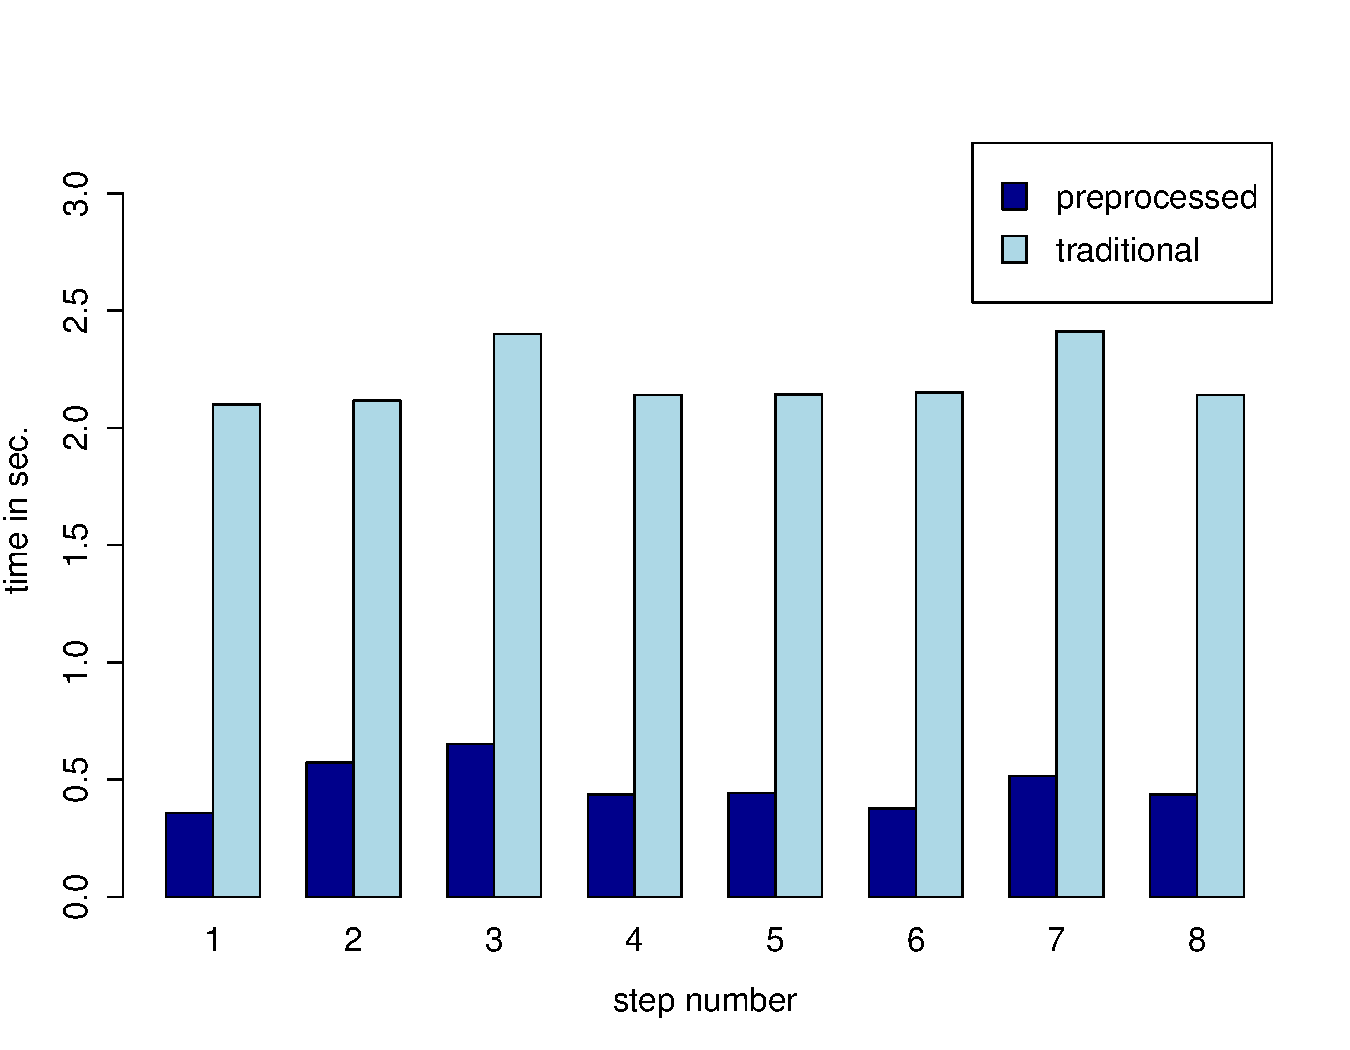
\includegraphics[width=0.5\textwidth]{Rplot26}
%     }
%   %  
%    % 
% %
% %
%     %}%\hfill
%     \subfloat[10 wards, reasoning time per event.\label{fig:results10ward}]{%
%       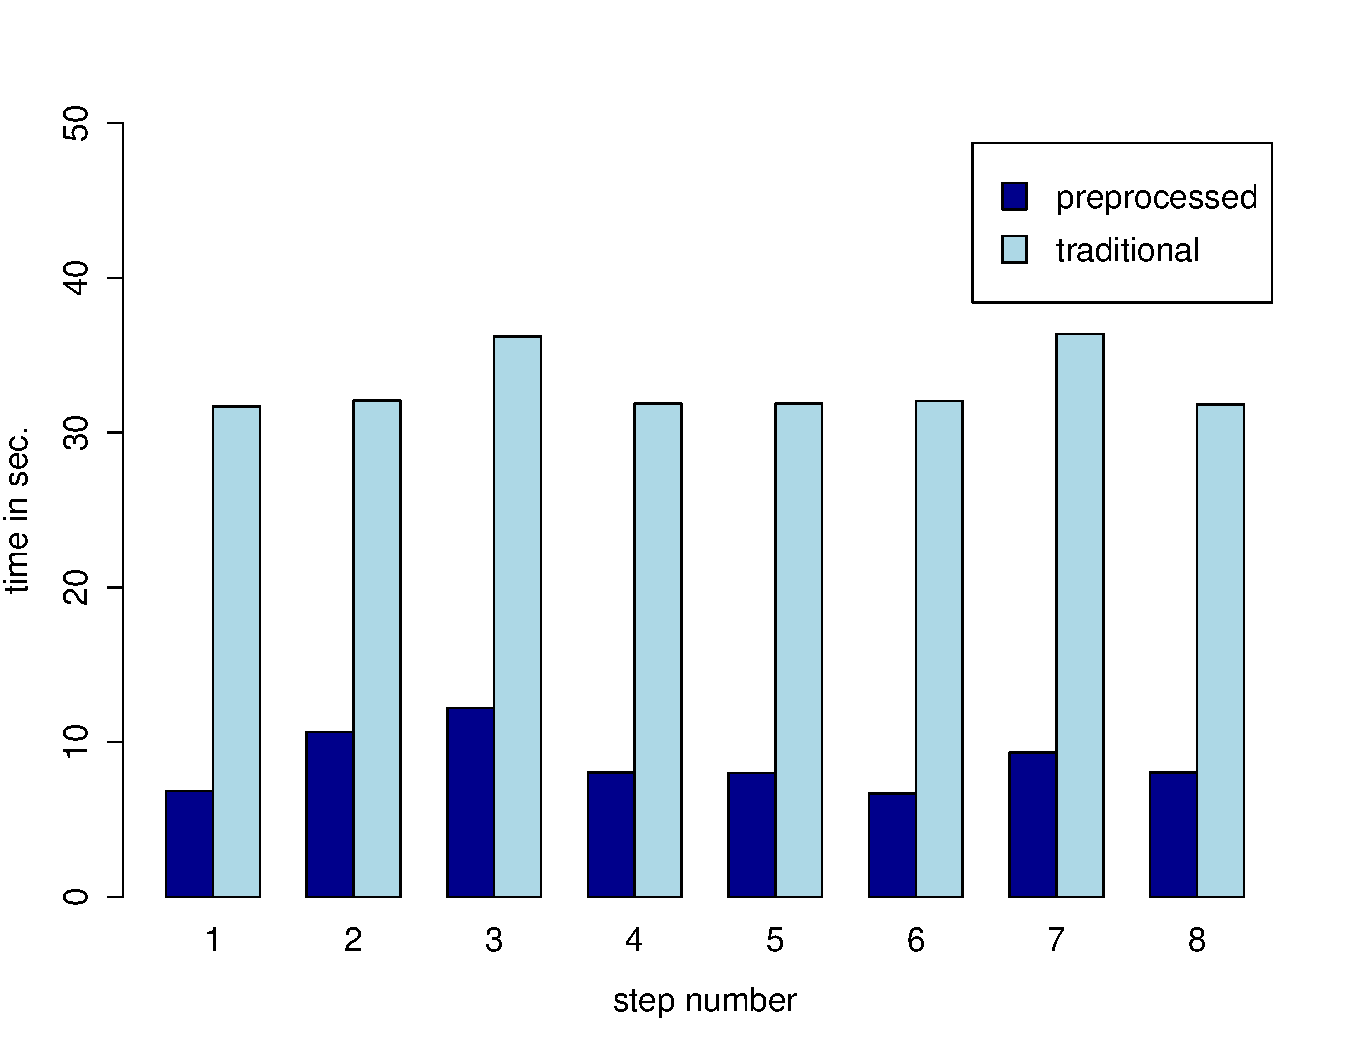
\includegraphics[width=0.5\textwidth]{Rplot27}
%     }
%     \caption{Comparison of reasoning times using preprocessed and traditional rules. The preprocessing step improves reasoning times.
%       }
%     \label{figure:results}
%   \end{figure}
%   
  

To better understand the impact of the preprocessing step, we further compare the reasoning times of the two implementations using \nthree. These are depicted 
in Figure~\ref{figure:results}.
The figure shows that preprocessing the rules improves reasoning times significantly,  consistently requiring only a quarter of the reasoning time.
This trend manifests itself regardless of the amount of dynamic data involved.
Whereas the traditional rule set can no longer be used in a hospital with 10 wards the 
preprocessed rule set still provides reasonable reasoning times. 
 \begin{figure}
\centering
\begin{subfigure}{.5\textwidth}
  \centering
  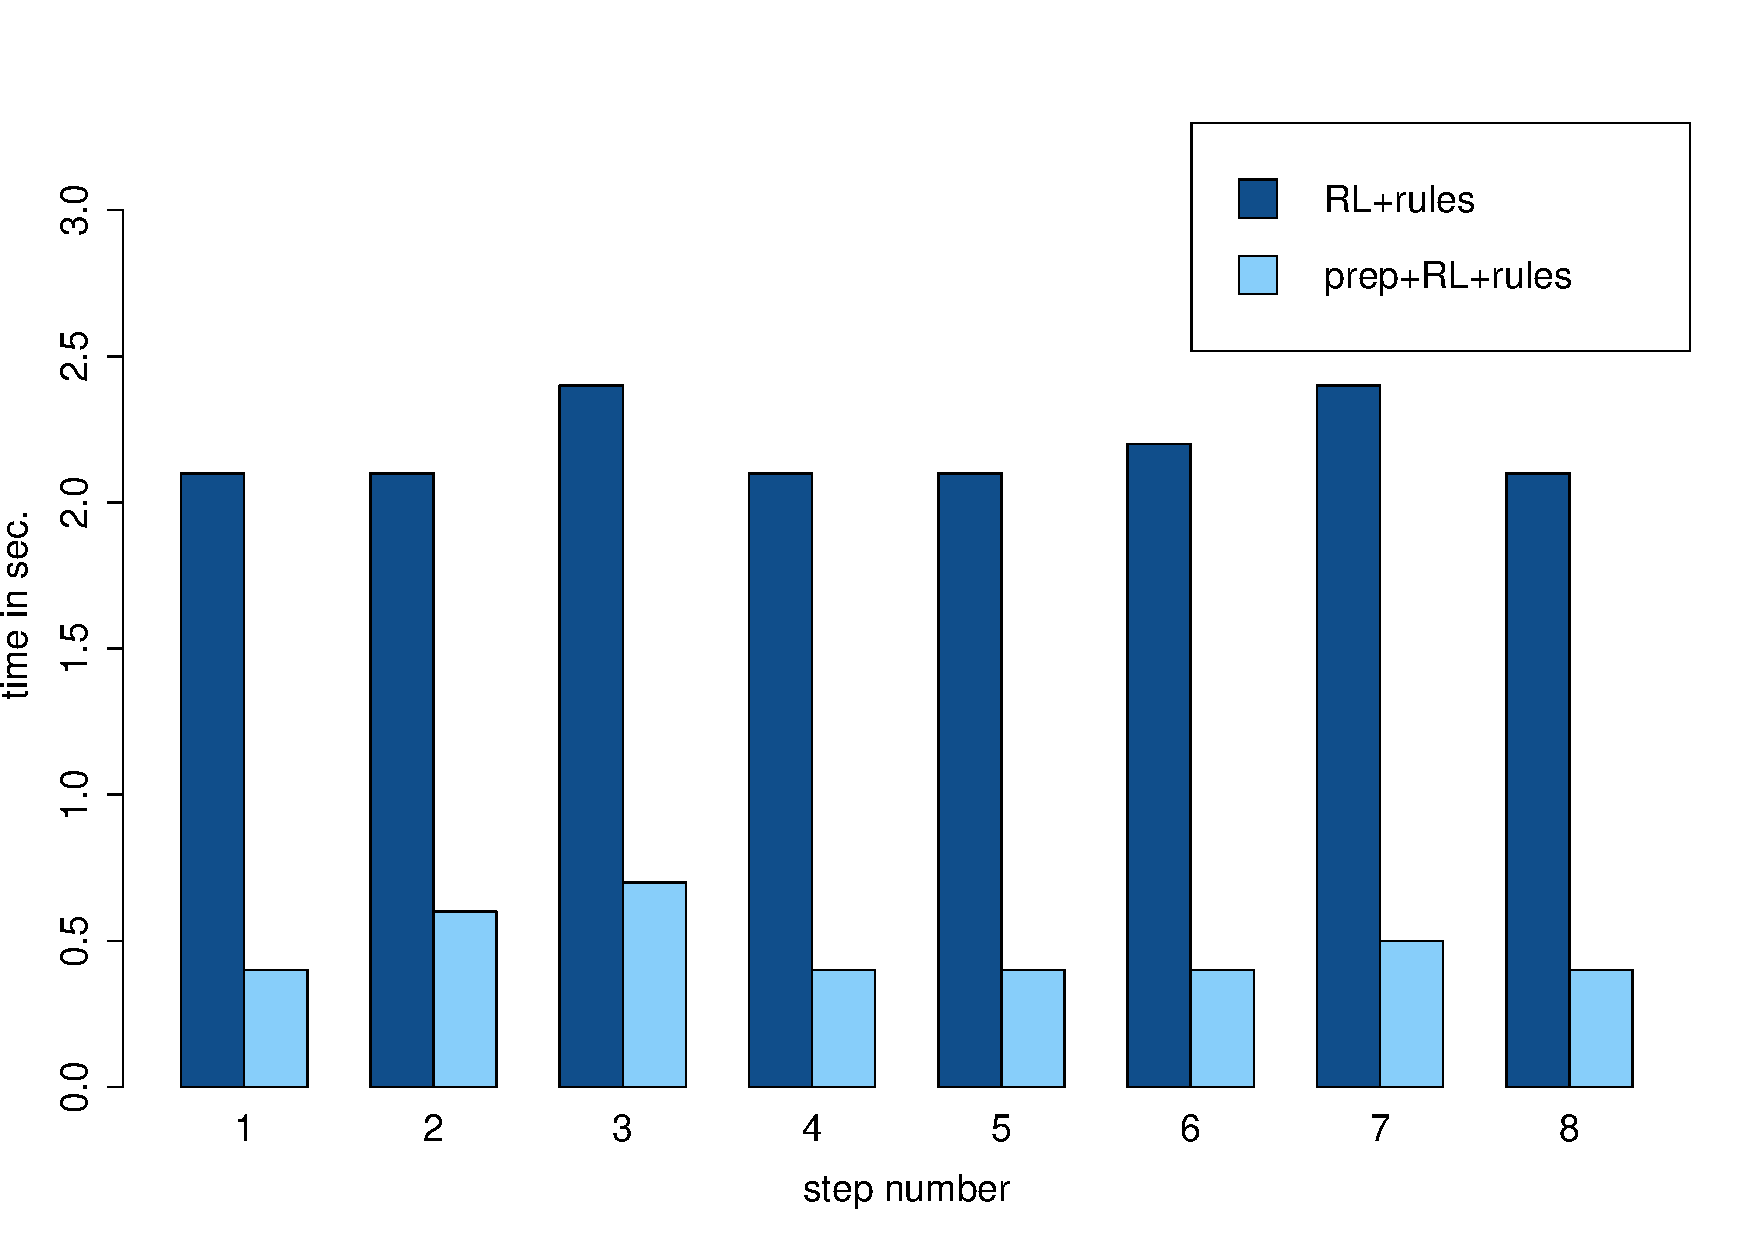
\includegraphics[width=\linewidth]{Rplot11}
  \caption{1 ward, reasoning time per event.}
  \label{fig:results1ward}
\end{subfigure}%
\begin{subfigure}{.5\textwidth}
  \centering
  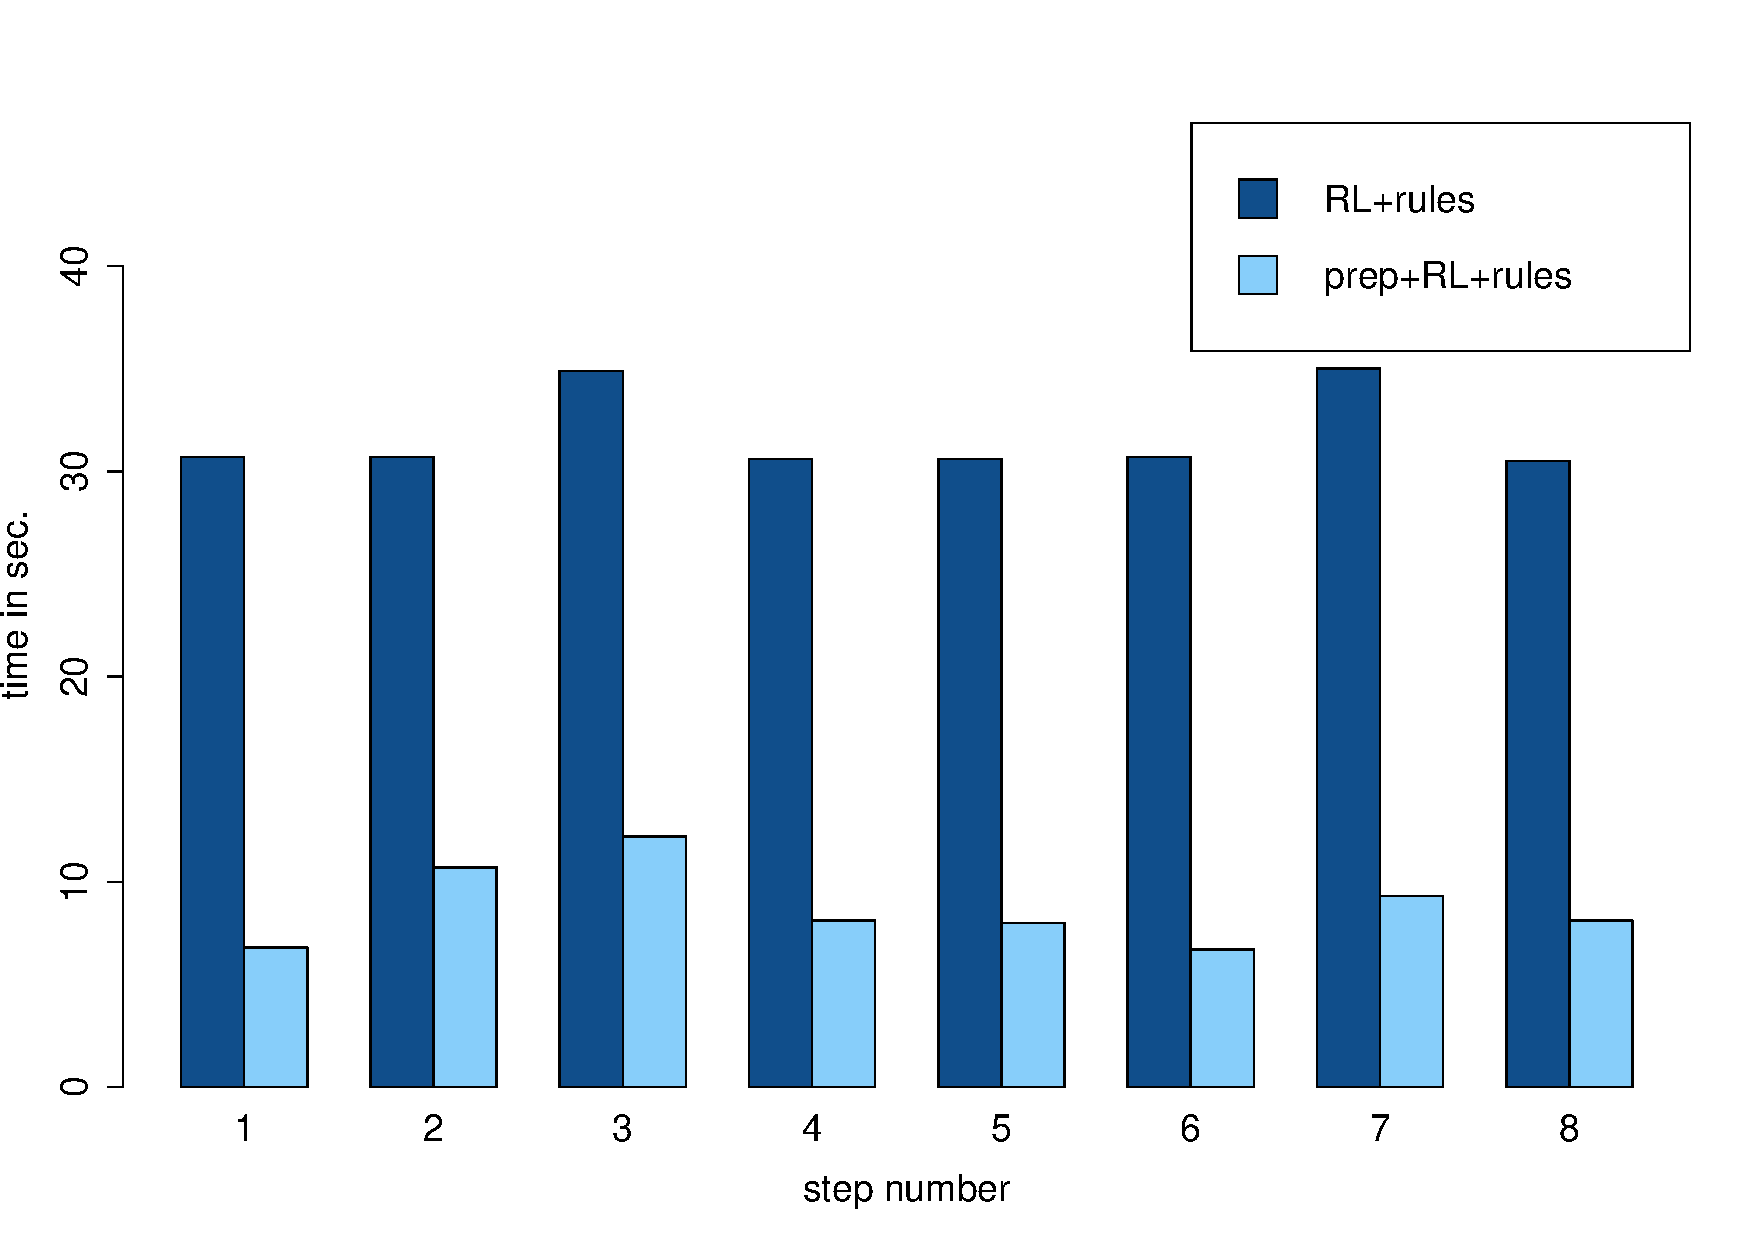
\includegraphics[width=\linewidth]{Rplot13}
  \caption{10 wards, reasoning time per event.}
  \label{fig:results10ward}
\end{subfigure}
\caption{Comparison of reasoning times using preprocessed and traditional RL rules in \nthree. The preprocessing step improves reasoning times.}
\label{figure:results}
\end{figure} 
 
\subsection{Discussion}
Our analysis has shown that the implementation using \owl RL and rules performs much faster than the one using OWL DL and SPARQL querying. The results could be 
further improved by using rule-producing rules, a special feature of \nthree. In this particular use case we can positively answer our initial question whether \nthree reasoning can 
solve the same practical problems as \owl DL reasoning and SPARQL querying with comparable performance. We can even say more: Here, the \nthree solutions outperform \owl DL and SPARQL.
But we also need to be careful: The OWL DL profile is of course more expressive than OWL RL and our good results were achieved by ignoring some derivations. 
In our use case these derivations were not relevant for the queries we wanted to answer and here we also see the actual advantage of using \nthree: We can customise the reasoning according to our needs.
From the various informations which are stated by means of an \owl DL ontology we chose which ones we wanted to use for further reasoning. If we need to be more expressive than \owl RL we can 
extend our rules set and use -- for example -- rules with new blank nodes in the consequent to support \owl ER \cite{owlex}, an \owl profile  which can be supported by existential rules. 
Powerful built-in functions provide us with even more options. By limiting the information we actually use for our conclusions, we can even reason over \owl Full ontologies 
and thereby accept an \owl format which is semantically compatible with \rdf.
% 
% 
% But these derivations 
% were not relevant for the queries we applied in our use case. Even though it was originally planned to solve the problem using OWL DL -- the ontology was created having this and 
% similar use cases in mind -- it was enough to only use OWL RL.  In our implementation we thereby chose which of the information available we want to use further snd here we also see the advantage 
% of using \nthree: OWL DL ontologies 

%semantic compatibility with \rdf.

% Above we compare the reasoning times of a very complex profile, \owl DL, with the less expressive profile \owl RL and it is therefore not surprising that the reasoning 
% is much faster.
% 
% I should say that we compared different things and that OWL DL is more expressive, but that the question here was rather focussed on practical cases and the conclusion we can draw is that we do not 
% always need OWL DL even when a solution was initially using that powerful profile. often, less expressive profiles are enough and these can be defined in a way which is semantically 
% compatible with \rdf.  
% 

%\section{Introduction}
%Modern nurse call systems should provide more than just sending a call to a nurse.


%\\ % We hereby propose a solution for this problem based on Notation3 rules.  %\\
%We use rule based reasoning on top of ontologies to implement this task.
%In a first attempt this problem was solved using an OWL \cite{OWL} ontology and SPARQL \cite{SPARQL} queries.
%To implement a nurse call system which meets these requirements, awareness of the context and  

%The solution we propose in this paper is based on an OWL \cite{OWL} ontology which we process using Notation3 \cite{notation3} rules.
%To implement a nurse call system which meets these requirements, we represented 




%\section{Background}\label{relwork}





\subsection{Business Case}\label{usecase}
Our business case is a nurse call system in a hospital.
The system is aware of certain details about personnel and patients.
Such information can include: personal skills of a staff member, staff competences, patient information, special patient needs, and/or the 
personal relationship between staff members and patients. %All this information is available in an OWL ontology. 
Furthermore, there is dynamic information available, as for example the current location of staff members and their status (busy or free). 
When a call is made, the nurse
call system should be able to assign the best staff member to answer that call. The definition of this ``best'' person
varies between hospitals and can be quite complex. 
Our system should thus be easily adjustable, but also very fast in taking a decision.
%\\
The system additionally controls different devices. If for example staff members enter a room with a patient, 
a decent light should be switched on; if they log into the room's terminal, they should have access to the medical lockers in the room. 
%
%By implementing such a system, 
Especially hospitals are interested in that kind of system as it enables them to organize their work 
%the work in a hospital can be organized 
in a more efficient way: 
\begin{itemize}
 \item Busy nurses get distracted less. They only receive a call if everyone else is also occupied or if the new task is more important than the task 
 they are currently performing.
 \item The system allows giving preference to staff members who are close to the caller. This prevents nurses from covering unnecessary big distances 
 in their anyhow stressful and physically exhausting 
 daily work.
 \item If the system is aware of the reason for a call, it can immediately assign nurses with the required skills. 
 Thus, no time is lost by first calling other staff members who then would have to ask for additional help.
 \item The system can prefer staff members who already know the patient and have a trust relationship with him. This increases the satisfaction of 
 the patient. At the same time, it also saves time for the caregiver, who is in such cases already familiar with the patient's needs and condition.
% \item The system keeps information about patients which can be assessed by the staff member called.
 \item The system is universal, i.e., electronic devices in the hospital can be controlled as well.
 \item The system is adaptable, i.e., hospitals can add their own requirements and priorities.
\end{itemize}

%Traditional nurse call systems don't take any patient-information into account. traditionally a patient makes a call and a random nurse responsible for the room gets the call.
%Our use case is different. We use all information available about a patient and the available nurses to always assign the best nurse (based on the current position of the nurse, the nurse's relation to the patient,
%competences, etc.) to the patient. Taking lots of information into account, such a system needs to be fast: especially in cases of emergencys the patient should not wait longer than number for the nurse.




\subsection{Technological Challenges}
\label{chal}
%Technological challenges - explaining why the business case is difficult to be solved by using traditional technologies

%Semantics: the system should be able to ``understand'' data and draw conclusions. \\
%Scalability: Huge datasets.\\
%Real-time: 5 seconds\\



An event-driven system as described above has to fulfill certain requirements. The system should:
%For the event driven system as described above we identified the following requirements:
%Below, we list the requirements (functional and non-functional) of the event-driven system of which we will devise a rule-based reasoning platform for. This system must
\begin{description}
%\item \emph{State} keep (consistent) state, which means it must be able to update data when an event is triggered,
\item[Scalability] cope with data sets ranging from 1000 to 100~000 relevant triple (i.e., triples necessary to be included for the reasoning to be correct);
\item[Semantics] be able to draw conclusions based on the information it is aware of;
\item[Functional complexity] implement deterministic decision trees with varying complexities; % from 1 to at least 6;
\item[Configuration] have the ability to change these decision trees at configuration time; and
\item[Real-time] return a response within 5 seconds to any given event.
\end{description}

%To meet these requirements different approaches can be taken.

%In a traditional hard coded system a fixed customized solution can be implemented. The main advantages of this approach are that they c 

There are several options to implement a nurse call system as described above. Following a more classical approach, the system could be written in 
an object-oriented programming language 
such as Java or C++. An implementation like this can easily fulfill the real-time and scalability constraints.
But such systems are traditionally hard-coded: they are implemented for a specific use case, and even though 
they might be able to support the required functional complexity, this implementation would be static. The possibility to configure complex decision trees
as postulated by the complexity requirement is rather hard to fulfill using traditional programming. Even more difficult to satisfy is the semantic requirement:
most object oriented languages do not support enough logic to ``understand'' the available information. Knowledge must be stated explicitly, 
as even simple connections between statements such as ``\textit{nurse x has location y}'' and ``\textit{y is location of nurse x}'' cannot be found easily.

Especially the last argument motivates us to solve the described problem using semantic web technologies as they natively fulfill the semantics requirement.
Knowledge can be represented in an OWL ontology which is understood by OWL-DL reasoners such as for example Pellet \cite{Pellet}. % or HermiT \cite{hermit}.
Complex decision trees can be handled by subsequent SPARQL queries. It is easy to add new queries or to change the order of existing queries 
and to thereby accommodate for the configuration constraint.
But our tests have shown that such systems inherently are not fast and reliable enough to fulfill the scalability and real-time requirements.
For bigger amounts of data or too complex decision trees, the reasoning times of traditional OWL-DL reasoners grow exponentially, which is not scalable.

To keep the benefits of an OWL-DL based implementation in a scalable and real-time way, we propose a rule-based solution.
By using OWL 2 RL rules and resolution instead of classical tableaux reasoning, we can significantly decrease reasoning times and still cover a major subset
of OWL 2. This approach benefits from the high performance of rule based reasoners. 
Even for bigger datasets the reasoning times are still faster than with the OWL-DL based approach. %very fast, as we will see later in this paper.  %and is able to reason very fast even over large datasets. 
%Because of its high performance (see benchmarks mentioned in \cite{eyepaper}), we chose the EYE reasoner for our purposes. As the reasoner is 
%able to cope with large datasets, our approach meets 
Also, complex decision trees can directly be implemented in rules. %, as those form the most natural 
As rules are the most natural representations of such trees, 
it is easy for a user to understand and change certain priorities 
or to configure new rules. A further advantage of our approach is that all logic is represented in one single way. Instead of
OWL plus SPARQL, we can implement the business case by only employing Notation3 Logic (N3). With the aforementioned system, we can meet all necessary requirements.
%, which makes our solution the 
%only one being able to fulfill all requirements.
%
%which form the most natu
%As this is the most natural representation
%Our implementation 
%Our solution is able to deal with 
%As the solution above, this implementation covers requirement \ref{sem}. 
%As we keep using 
%Our approach uses knowledge still makes use of 
%
%Our implementation makes use of OWL-RL rules written in Notation3. % \cite{notation3}.  
%As these rules enable us to cope with knowledge stored in OWL ontologies, our approach is general enough
%to be compatible with other semantic systems. 
%As the approach described above, requirement \ref{sem} 
%For our specific use case, OWL-RL was expressive 
%enough the provide the same results as a comparable OWL-DL based solution.
%
%Even though OWL-RL is less expressive than OWL-RL, this difference 
%had no influence to our use case. 
%Our system uses the EYE reasoner \cite{eyepaper} 
%The performance
%of the reasoner 
%whose high performance enables us to significantly increase the reasoning speed compared to an OWL-DL based solution.
%We additionally implemented the decision tree using rules. As rules are the natural representation of decision trees, 
%it is easy for the user to change certain priorities 
%or to add new rules.
%
%Instead of SPARQL-queries, a rule based solution can s


%PROS
%\begin{itemize}
% \item faster than owl
% \item one logic for all, no combination between OWL and query language
% \item EYE is very performant!
%\end{itemize}

 
 

%will especially have problems to meet the ``configuration''-requirement. A change in the decision tree would mean a change in the program code. 
%It is rather difficult to change 
%If a system is implemented in a traditional programming language for a specific use case it is 
%always difficult to change 


%Hard coded systems are not able to ``understand'' the data they are aware of. 


%A traditional hard coded system could not cope with

%A system as described above has to deal with a huge amount of knowledge, it has to reason about that knowledge and is must be able to update its own information 
%according to its conclusions (if a nurse is in a patients room, he is probably not ``free or available'' any more). As every hospital is different, 
%the rules or preferences in which kind of situation which nurse should be called also differs. 
%Our system should be easily adaptable. All this decisions must be taken real time.

%Traditional hard coded systems lack in particular the second last requirement: They are normally not flexible enough. A customized solution
%for a particular use case

%Traditional hard coded systems have problems to fulfill all the requirements mentioned above:
%Traditional hard coded systems are not flexible enough to fulfill these requirements. 
%The are not able to draw conclusions from huge datasets. 

%Although hard coded systems might be able to deal with a huge amount of data, they will not be 
%able to ``understand'' changes in the data and the possible consequences. Furthermore such systems lack the possibility to be changed at configuration time. Every new 
%requirement would require a new implementation of the system.

% Semantic based systems using purely OWL reasoning are on the other hand really good in 
% 
% 
% %Traditional hard coded systems can not easily incorporate all data needed. They are not flexible enough to ``understand'' complex situations. 
% %Rules which staff members should be called in what situations cannot be adapted that easily. 
% 
% Representing knowledge in OWL-ontologies is already an improvement but pure OWL-DL reasoning is too complex for this particular use case.
% Previous tests showed that by only using OWL-2 reasoners without any additional strategies we do not meet the time constraints
% of the real business use case. We need a powerful, but in the meantime fast solution.
% 
% 
% 
% 
% Analysis of the use case gave specifications as listed below.
% \begin{enumerate}
% \item Only a subset of the data is susceptible to change when an event is triggered, and this subset can be defined at initialization time. This subset is quite small (i.e., around $15\%$, irrespective of the total size of the data set), and is clearly defined as only a couple of classes and predicates that introduce dynamic data.
% \item There are events that trigger a state change before any reasoning needs to be done (e.g., a worker walks away from a certain location to another), and there are (similar) events that trigger a state change after the reasoning is done (e.g., a worker walks from his office to the complaint desk, meaning his status changes from 'free' to 'handlingClient').
% \item This reasoning system needs (thus) to be able to cope with state, and more specifically, be able to update a state based on reasoning.
% \item The change of a state is also part of a decision tree (e.g., when a worker is busy with a certain complaint, and he changes location, for example to get a file, consensus is needed whether his status changes from 'handlingClient' to 'away' or not. This consensus could be different for different companies).
% \end{enumerate}
% 
% Conclusions that can be drawn of these observations are as follows:
% \begin{enumerate}
% \item Preprocessing the static data at initialization time can give a significant performance gain, as this preprocessed optimized static data set can be reused every time an event is triggered.
% \item An event-driven reasoning system needs to be able to (programmatically) update the state of the data twice: once before the reasoning, and once after the reasoning. This preliminary update is necessary to avoid having conflicting data states (e.g., a worker being at two distinct locations at the same time when a reasoning occurs).
% \item This second update needs to keep track of the timestamp of when an event was triggered to cope with states that change through reasoning. explain better
% \item Each event actually introduces two reasoning runs: one for the actual reasoning over the event, and one to update the state. This second update also needs to be done by reasoning, as otherwise, the change between states is implemented programmatically, and can no longer be configured at configuration time.
% \end{enumerate}
% 
% Some specific other remarks due to the used technology stack:
% \begin{itemize}
% \item As the EYE-reasoner is a file-based process, the entire application needs to work file-based to persist its state. This also means that for every event, the current state needs to be updated in a file, which introduces some overhead compared to keeping the state in memory.
% \item As each event introduces two reasoning runs, this mean this file reading and writing overhead by EYE is doubled.
% \end{itemize}










\subsection{Rule-based Solution}\label{details}

%Technical details of the rule based solution

%Rule-based solution - technical details, esp. the usage of rules

%We use rules for two things: first to do owl-RL reasoning, second: to do the query. 
In this section, we further explain our solution in three parts.
First, we focus on the technical background and the technologies used. %give %an introduction into the technologies used and explain our choices. %first we give a brief introduction into N3 and the EYE-reasoner. 
In the second part we describe 
how we could improve reasoning times for our use case by employing OWL 2 RL rules written in N3. 
In the third part we show example rules from our decision trees and discuss options to change these rules. %, to give an idea how rules can be changed.

\subsubsection{Background}
Our solution improves on a more classical implementation which employs the OWL 2 reasoner Pellet \cite{Pellet}, and where
the decision tree was implemented via SPARQL queries.
All knowledge was represented using the ACCIO ontology\todo{name!}, which is described %a description is given 
by Ongenae et al. \cite{accioont}. 
Knowledge could either be fixed or dynamic, and updated via an event.
Fixed knowledge is, for example, information about skills of staff members, or patients' preferences.
Dynamic knowledge is, for example, the movement
of a nurse to a certain location, or a new call which is made by a patient.

%From the former implementation we keep the
Our new implementation keeps the knowledge representation of the first attempt but replaces SPARQL and OWL by Notation3 Logic (N3) \cite{N3Logic}.
%The only thing we keep from that former approach in our rule based implementation is 
%We have two kinds of knowledge, 
%We have two sources of knowledge: a static database translated into owl contains all information about staff, patients and physical devices which can be known beforehand. 
%Furthermore we
This logic forms a superset of \rdf and extends the \rdf data model by formulas (graphs), functional predicates, universal variables and logical operators, in particular
the implication operator. %extends the RDF model by adding formulas (literals which are graphs themselves), 
%variables, logical implication, and functional predicates. %, as well as providing an textual syntax alternative to RDF/XML.
These last two features enable the user to express rules. %can be understood by a reasoner.
As %a Notation3 
reasoner we use EYE \cite{eyepaper}, a semibackward reasoning engine enhanced with Euler path detection. 
The main reason for our choice is the high performance of the reasoner. Existing benchmarks and results are listed on the EYE website \cite{eye}. %Eye is especially
%
%The knowledge is represented in an OWL ontology \cite{accioont}
%Explain: Simple example. The reasoner needs a query.
%EYE \cite{eyepaper}.

%\subsection{Representing the knowledge}


\subsubsection{OWL 2 RL in N3}
%We started from an OWL-DL ontology which was used to 
%Possible data which can be processed by our system  
%The ACCIO Ontology
To be able to support OWL 2 RL reasoning in N3 we used the OWL 2 RL/\rdf rules as listed on the corresponding website~\cite{OWLRL}. 
Where possible, we made use of existing N3-translations of these rules as provided by EYE~\cite{EYEowl}. 
Missing concepts were added. Although the ACCIO ontology is designed for OWL-DL reasoning, the limitation to OWL RL had no impact for 
our specific use case. %, all derivations needed to cope with the desired decision trees were supported by OWL RL. 


\begin{lstlisting}[
  float=t,
  caption={OWL-RL rule for \texttt{rdfs:subClassOf} class axiom in N3.},
  label=lst:subclass]
§\textcolor{gray}{@prefix rdfs: <http://www.w3.org/2000/01/rdf-schema\#>.}§
§\textcolor{gray}{@prefix rdf: <http://www.w3.org/1999/02/22-rdf-syntax-ns\#>.}§

{?C rdfs:subClassOf ?D. ?X a ?C} => {?X a ?D}.
\end{lstlisting}
To illustrate the idea of using rules for OWL reasoning, we give a small example: Listing~\ref{lst:subclass} shows 
the class axiom rule\footnote{The rule is the N3 version of the cax-sco rule in Table 7 on the OWL 2 Profiles website~\cite{OWLRL}.} which is needed 
to deal with the rdfs concept
 \verb!subclassOf!. For convenience we omit the prefixes in the formulas below. The empty prefix refers to the ACCIO ontology, 
 \verb!rdf! and \verb!rdfs! have the same meaning as in Listing~\ref{lst:subclass}. Consider that we have the following T-Box triple stating that the class \verb!:Call!
 is 
 a subclass of the class \verb!:Task!:
 %If the ontology contains the triples
\[
 \verb!:Call rdfs:subClassOf :Task.! \tag{1}\label{1}
\]
If the A-Box contains an individual which is member of the class \verb!:Call!
\[\verb! :call1 a :Call.! \tag{2}\label{2}\]
%a rule based reasoner can use the rule given in listing \ref{lst:subclass} to conclude 
an OWL DL reasoner would make the conclusion that the individual also belongs to the class \verb!Task! 
\[
 \verb!:call1 a :Task.! \tag{3}\label{3}
\]
Our rule in Listing \ref{lst:subclass} does exactly the same: as Formula~\ref{1} and Formula~\ref{2} can be unified with the antecedence of the rule, a reasoner derives
the triple in Formula~\ref{3}. Other concepts can be handled similarly.







\subsubsection{Decision Trees }




 


%REMARK: Still not sure whether we need this section?
%The decision trees which have to be implement
%As mentioned above, decision trees as needed in for real life use cases can be quite complex. 

%Depending on the amount of available information, decision trees for nurse call systems can be quite complex. The ACCIO ontology 
%supports a huge variety of different concepts. %It is possible to model the profile of a patient (among others the 
 
The ACCIO ontology~\cite{accioont} provides the user with a huge variety of concepts which can, e.g., be used to describe patients (social background, needs, disease), 
staff members (skills, relationships to patients), and situations (locations of persons, states of devices). If all this information is actually available, decision trees
can use all of it and be therefore quite complex. In this section we provide two simple rules which could be part of such a tree and we explain how these rules can
be modified depending on the needs of an individual hospital.
 
 \begin{lstlisting}[
  float=t,
  caption={Rule assigning a preference value to a staff member with status "free" who is close to the call-location. },
  label=lst:ex]
§\textcolor{gray}{@prefix : <http://ontology/Accio.owl\#>.}§
§\textcolor{gray}{@prefix rdf: <http://www.w3.org/1999/02/22-rdf-syntax-ns\#>.}§

{
  ?c rdf:type :Call.
  ?c :hasStatus :Active. 
  ?c :madeAtLocation ?loc. 
  ?p :hasRole [rdf:type :StaffMember].
  ?p :hasStatus :Free.
  ?p :closeTo ?loc.
}
=>
{
  (?p ?c) :assigned 200.
}.
\end{lstlisting}
 
Listing~\ref{lst:ex} shows a rule which, given an active call, assigns a staff member with a certain preference to that call. The EYE reasoner works 
with filter rules (queries), it is easy to search for the assignment of a staff member with the lowest or highest number. 
In our example, lower numbers mean higher preferences. The antecedence of the given rule contains certain constraints: the active call is made on a certain location and
there is a staff member, who is currently free and close to that location. In such a case, our rule assigns the number 200 to the combination of call and staff member.

\begin{lstlisting}[
  float=t,
  caption={Rule assigning a preference value to a busy staff member who has the needed skills to answer the call. },
  label=lst:ex2]
§\textcolor{gray}{@prefix : <http://ontology/Accio.owl\#>.}§
§\textcolor{gray}{@prefix rdf: <http://www.w3.org/1999/02/22-rdf-syntax-ns\#>.}§

{
  ?c rdf:type :Call.
  ?c :hasStatus :Active.
  ?c :hasReason [rdf:type :CareReason].
  ?p rdf:type :Person.
  ?p :hasStatus :Busy.
  ?p :hasRole [rdf:type :StaffMember].
  ?p :hasCompetence [rdf:type :AnswerCareCallCompetence].
}
=>
{
  (?p ?c) :assigned 100.
}.
\end{lstlisting}








Listing~\ref{lst:ex2} displays another rule: here, the reason of the active call is known. We have a staff member who has the required 
skills to answer that kind of calls, but this staff member is currently busy. Our rule assigns the number 100 to this
combination of call and staff member. This means, in our current decision tree, we prefer this assignment to the one described by Listing~\ref{lst:ex}.

Now, it could be, that another hospital has different priorities. Imagine for example that in this new hospital, no busy staff should be called 
if there is still a free staff member available, regardless of the reason of the call. We could easily adapt our decision tree by simply changing the assignment number 
of one of the rules. If we replace the triple \[\verb! (?p ?c) :assigned 100.!\] in line 16 of Listing \ref{lst:ex2} by the triple \[\verb! (?p ?c) :assigned 300.!\]
the reasoner would prefer the assignment expressed by Listings \ref{lst:ex} to~\ref{lst:ex2}.

 
Similarly, we can add extra conditions to the rules. Currently, the rule in listing \ref{lst:ex2} does not take the location of the staff member into account. We can
change that by only adding the triples 
\[ \verb!?c :madeAtLocation ?loc. ?p :closeTo ?loc.!\]
to the antecedence of the rule. To give this new rule a higher priority than the existing one, we would again only have to change the assigned number in the consequence.
Rules with the same number are treated equally.















\subsection{Results}\label{ev}
%Results - the benefits of the solution, including improvement of KPIs


We compared the reasoning times of our implementation with the results of our former implementation using 
the Pellet reasoner and subsequent SPARQL-queries. 
As a joint test set up we ran a sequence of events, which we list below, the expected reasoning result is indicated in brackets. 

\begin{enumerate}
\item %[Launch Call] 
A patient launches a call (\emph{assign nurse and update call status})
\item
%[Redirected Call] 
The assigned nurse indicates that she is busy (\emph{assign other nurse})
\item
%[Temporarily Accept Call] 
The newly assigned nurse accepts the call task (\emph{update call status})
\item %[Corridor] 
The nurse moves to the corridor (\emph{update location})
\item %[Patient room] 
The nurse arrives at the patients' room (\emph{update location, turn on lights  and update nurse status})
\item %[Log in] 
The nurse logs into the room's terminal (\emph{update status call and nurse, open lockers})
\item %[Log off] 
The nurse logs out again (\emph{update status call and nurse, close lockers})
\item %[Corridor] 
The nurse leaves the room (\emph{update location and call status and turn off lights})
\end{enumerate}

We tested this set-up for two datasets, one dataset consisting of the nurses, hospital rooms and patients of one single ward, the other one for 10 wards.
Figure~\ref{fig:summary} shows the difference in reasoning times of this use case on the same hardware settings\footnote{Debian ``'Wheezy'', Intel(R) Xeon(R) CPU E5620@2.40GHz, 12GB RAM}, using two different technology stacks: the Pellet+SPARQL installation vs. the EYE installation\footnote{Pellet 3.0 and OWL-API 3.4.5 vs. EYE 7995 and SWI-Prolog 6.6.6}.
The timings shown are the sum of all reasoning cycles.

As the figure shows, the reasoning times of EYE are almost one order of magnitude better than the reasoning times of Pellet+SPARQL. 
When we review the reasoning times per call for one ward (Figure~\ref{fig:results1ward}), we see that the EYE installation has far 
more predictable reasoning times, as it is more robust against more complex decision trees
(e.g., the decision trees of the first two events are notably more complex than the other events' decision trees).
Pellet+SPARQL is much faster than EYE in the third event, because this event does not trigger any reasoning for Pellet+SPARQL, however, 
%in the EYE implementation a full reasoning cycle is performed for every incoming event.
a full reasoning cycle is performed by EYE. 
With an average reasoning time of about 2 seconds, the real-time constraint is achieved within small-scale datasets.

%\begin{figure}
% \small
% \begin{tabular}{p{1.3cm} p{1cm} p{1cm}}
% \hline
% \# wards & EYE & Pellet\\
% \hline
% \hline
% 1 & 18 & 79\\
% 10 & 288 & 2~124\\
% \hline
% \end{tabular}
% \normalsize
%\end{figure}



% \begin{figure}
% \begin{center}
% \includegraphics[width=0.7\textwidth]{Rplot18.jpeg}
% \end{center}
% \caption{Comparison of reasoning times of the individual events for 1 ward. EYE is generally faster, and more predictable.}
% \label{fig:results1ward}
% \end{figure}












%   \begin{figure}[!ht]\centering
% %  \CenterFloatBoxes
%  % \begin{floatrow}
%     \subfloat[Sum of reasoning times. % in seconds.
%     \label{fig:summary}]{
% % \begin{tabular}[b]{|l| r | r |}
% % \hline
% %  & 1 ward & 10 wards \\
% %  \hline
% %  \hline
% %  Pellet + SPARQL & 78.9 s & 2~124.1 s\\
% %  \hline
% %  EYE & 17.7 s & 287.7 s \\
% %  \hline
% %  \multicolumn{1}{c}{} \\
% %  \multicolumn{1}{c}{}
% % \end{tabular}
% 
% \small
% \begin{tabular}[b]{p{1.4cm} p{1cm} p{1cm}}
% \hline
% 
% No. of & \multicolumn{2}{c}{Time in sec.}\\
% %wards &\multicolumn{2}{c}{(in sec)} \\
%  wards & EYE & Pellet\\
% \hline
% \hline
% 1 & 18 & 79\\
% 10 & 288 & 2~124\\
% \hline
% &&\\
% &&\\
% &&\\
% \end{tabular} 
% \
% % \begin{tabular}[b]{|l| r | r |}
% % \hline
% %  & 1 ward & 10 wards \\
% %  \hline
% %  \hline
% %  Pellet + SPARQL & 78.9 s & 2~124.1 s\\
% %  \hline
% %  EYE & 17.7 s & 287.7 s \\
% %  \hline
% %  \multicolumn{1}{c}{} \\
% %  \multicolumn{1}{c}{}
% % \end{tabular}
% 
% \normalsize
% 
%     }\hfill
%     \subfloat[1 ward, reasoning time per event.\label{fig:results1ward}]{%
%       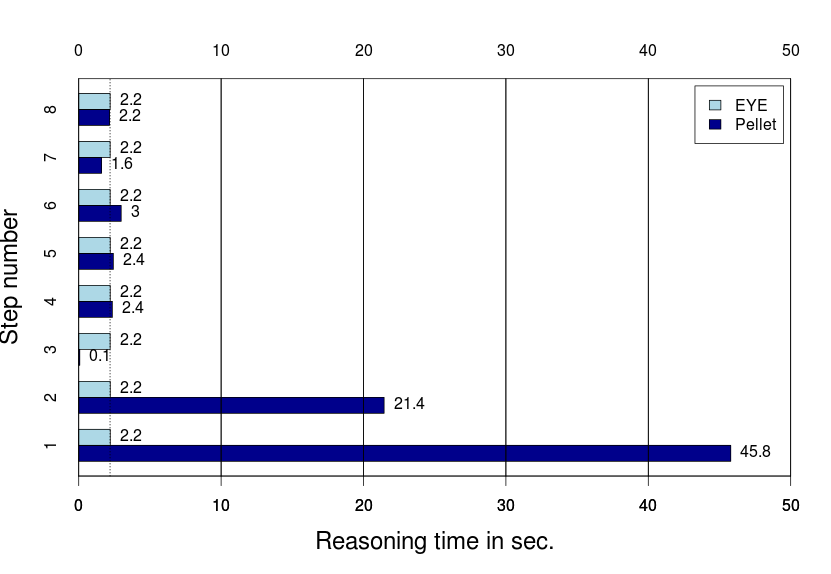
\includegraphics[width=0.6\textwidth]{Rplot14.png}
%     }
%     \caption{Comparison of reasoning times. EYE is generally faster, and more predictable.}
%     \label{figure:results} %\end{floatrow}
%   \end{figure}
  
 \begin{figure}
\centering
\begin{subfigure}{.4\textwidth}
  \centering
  {
% \begin{tabular}[b]{|l| r | r |}
% \hline
%  & 1 ward & 10 wards \\
%  \hline
%  \hline
%  Pellet + SPARQL & 78.9 s & 2~124.1 s\\
%  \hline
%  EYE & 17.7 s & 287.7 s \\
%  \hline
%  \multicolumn{1}{c}{} \\
%  \multicolumn{1}{c}{}
% \end{tabular}

\small
\begin{tabular}[b]{p{1.4cm} p{1cm} p{1cm}}
\hline

No. of & \multicolumn{2}{c}{Time in sec.}\\
%wards &\multicolumn{2}{c}{(in sec)} \\
 wards & EYE & Pellet\\
\hline
\hline
1 & 18 & 79\\
10 & 288 & 2~124\\
\hline
&&\\
&&\\
&&\\
\end{tabular} 
\
% \begin{tabular}[b]{|l| r | r |}
% \hline
%  & 1 ward & 10 wards \\
%  \hline
%  \hline
%  Pellet + SPARQL & 78.9 s & 2~124.1 s\\
%  \hline
%  EYE & 17.7 s & 287.7 s \\
%  \hline
%  \multicolumn{1}{c}{} \\
%  \multicolumn{1}{c}{}
% \end{tabular}

\normalsize

    }
  \caption{Sum of reasoning times.}
  \label{fig:summary}
\end{subfigure}%
\begin{subfigure}{.6\textwidth}
  \centering
  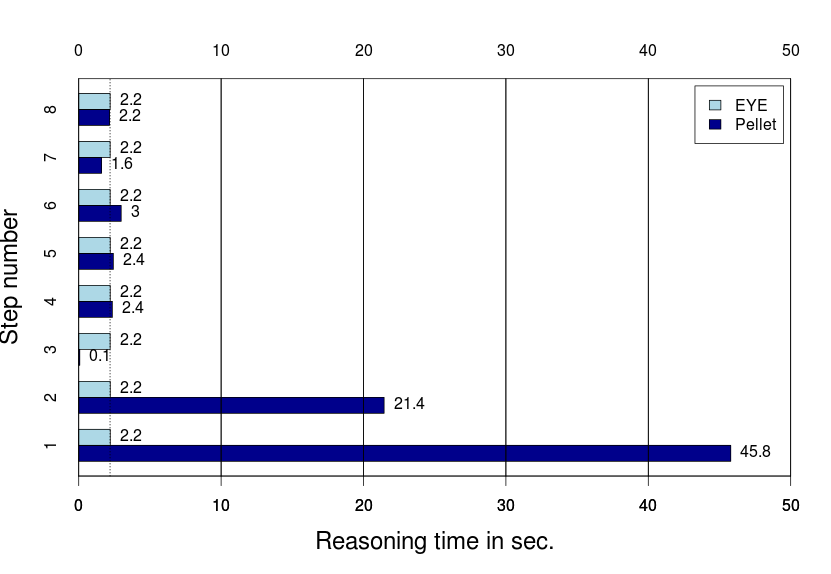
\includegraphics[width=\linewidth]{Rplot14.png}
  \caption{1 ward, reasoning time per event.}
  \label{fig:results1ward}
\end{subfigure}
\caption{Comparison of reasoning times. EYE is generally faster, and more predictable.}
\label{figure:result}
\end{figure} 
  
  
  
%     \begin{figure}[!ht]
%    \subfloat[1 ward\label{subfig-1:dummy}]{%
%       \begin{tabular}[t]{ccc}
% \hline
% \# wards & EYE & Pellet\\
% \hline
% \hline
% 1 & 18 & 79\\
% 10 & 288 & 2~124\\
% \hline
% \end{tabular}
%     }
%     \hfill
%     \subfloat[10 wards\label{subfig-2:dummy}]{%
%       \includegraphics[width=0.4\textwidth]{Rplot15.png}
%     }
%     \caption{Comparison of reasoning times of the individual events. EYE is generally faster, and more predictable.}
%     \label{table:results}
%    
%   \end{figure}
  
  
 
  

  
  
	


% 
% \begin{figure}
% \centering
% \begin{minipage}[t]{.4\textwidth}
% \centering
% \vspace{0pt}
% \includegraphics[width=0.5\textwidth]{Rplot15}
% \caption{This is the caption for figure}
% \end{minipage}\hfill
% \begin{minipage}[t]{.4\textwidth}
% \centering
% \vspace{0pt}
% \captionof{table}{This is the caption for table}
% \begin{tabular}{cc}
% 1 & Item 1 \\
% 3 & Item 2 \\
% 4 & Item 3 \\
% 5 & Item 4 \\
% 5 & Item 5 \\
% \end{tabular}
% \end{minipage}
% \end{figure}
%

  
  
  
  
  
%   \begin{figure}
%   \begin{minipage}[b]{0.6\linewidth}
%     \centering
%     %\includegraphics[width=\linewidth]{example-image}
% 
%  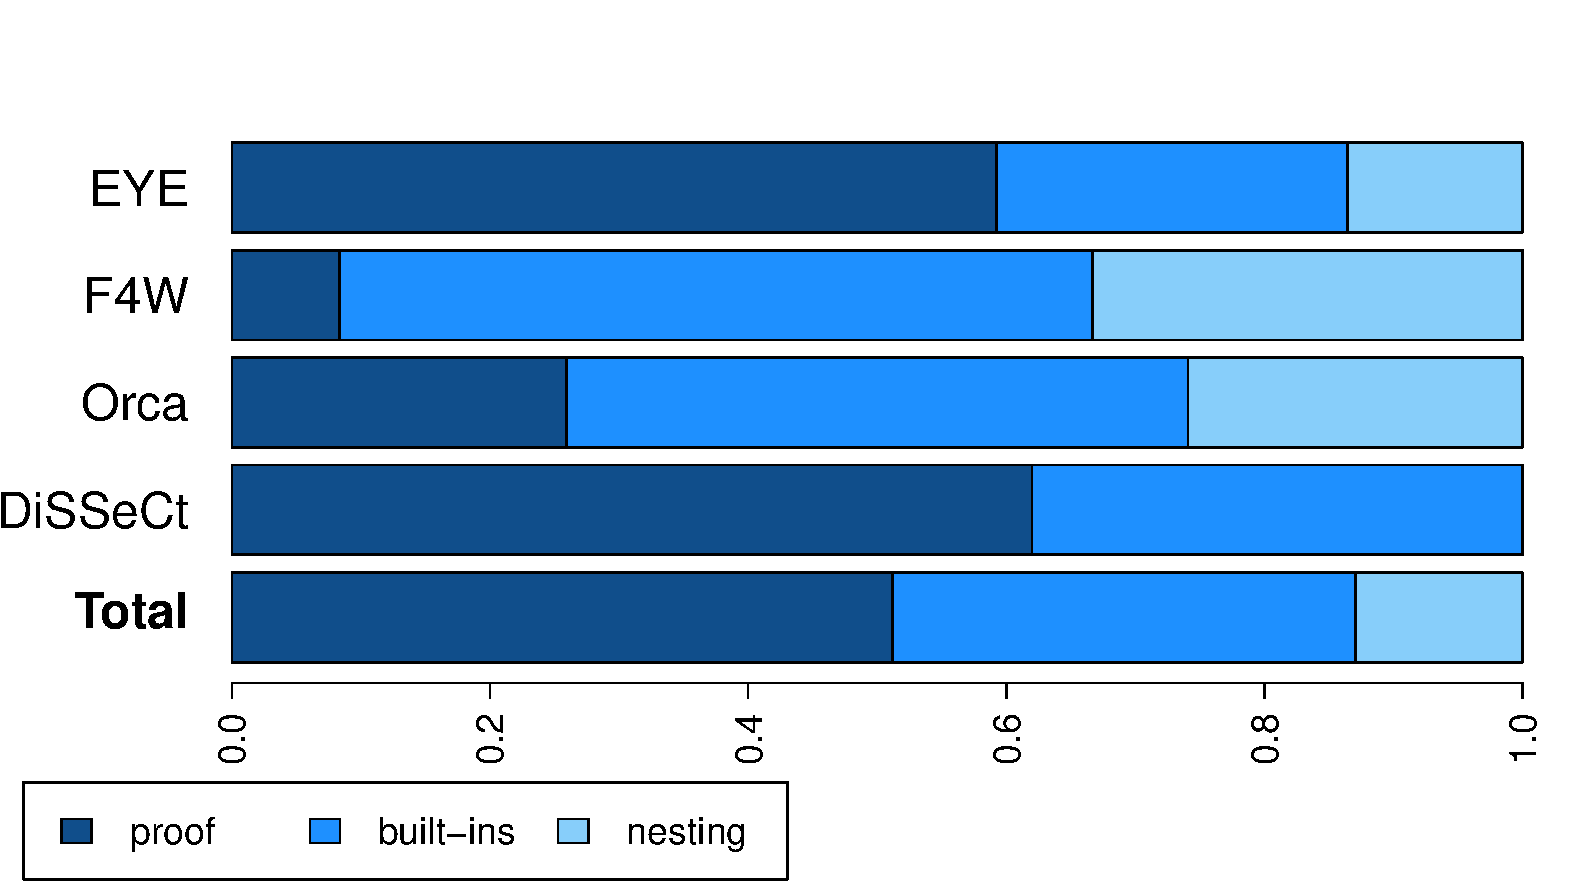
\includegraphics[width=\textwidth]{Rplot14}
% %\hspace{3cm}
%     %\rule{6cm}{6cm} %to simulate an actual figure
%   \caption{Comparison of reasoning times for individual events, 1 ward. EYE is generally faster, and more predictable.}  \label{fig:results1ward}
%   \end{minipage}%
%   \begin{minipage}[b]{0.3\linewidth}
%     \centering
%     \small
% \begin{tabular}{p{1cm} p{1cm} p{1cm}}
% \hline
% Wards & EYE & Pellet\\
% \hline
% \hline
% 1 & 18 & 79\\
% 10 & 288 & 2~124\\
% \hline
% &&\\
% &&\\
% \end{tabular} 
% \normalsize
% \caption{Comparison of the overall reasoning time for both, 1 and 10 wards. Values in seconds.}\label{fig:summary}
% \end{minipage}
% 
% \label{fig:test}
% \end{figure}
  
  
  
  
  
  
%   
  
%  \begin{figure}
%         \centering
%         \begin{subfigure}[b]{0.5\textwidth}
% \small
% \begin{tabular}{p{1.3cm} p{1cm} p{1cm}}
% \hline
% \# wards & EYE & Pellet\\
% \hline
% \hline
% 1 & 18 & 79\\
% 10 & 288 & 2~124\\
% \hline
% \end{tabular}
% \normalsize
%                 %\includegraphics[width=\textwidth]{gull}
%                 \caption{summary}
%                 \label{fig:summary}
%                 
%         \end{subfigure}%
%         ~ %add desired spacing between images, e. g. ~, \quad, \qquad, \hfill etc.
%           %(or a blank line to force the subfigure onto a new line)
% %         \begin{subfigure}[b]{0.3\textwidth}
% %                 \includegraphics[width=\textwidth]{tiger}
% %                 \caption{A tiger}
% %                 \label{fig:tiger}
% %         \end{subfigure}
%         ~ %add desired spacing between images, e. g. ~, \quad, \qquad, \hfill etc.
%           %(or a blank line to force the subfigure onto a new line)
%         \begin{subfigure}[b]{0.5\textwidth}
%                 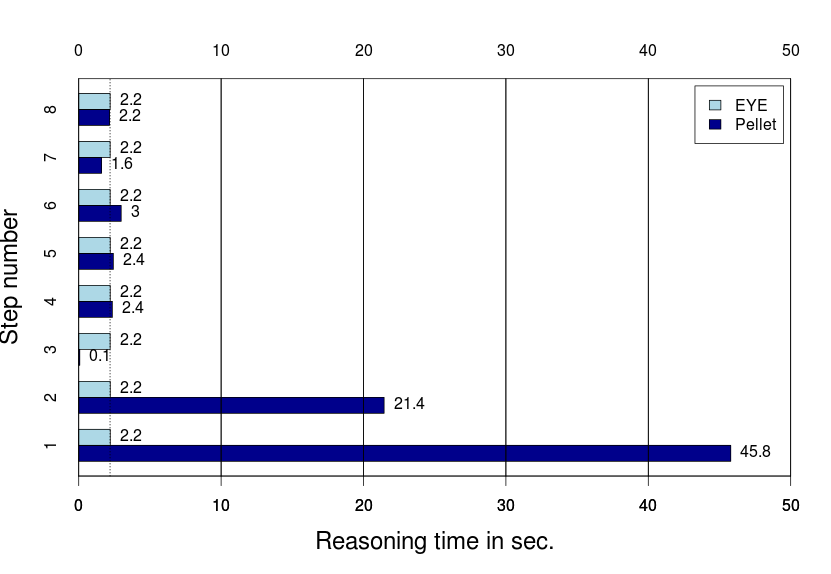
\includegraphics[width=\textwidth]{Rplot14.png}
%                 \caption{1 ward}
%                \label{fig:results1ward}
%         \end{subfigure}
%         \caption{Comparison of reasoning times (all numbers in seconds). EYE is generally faster, and more predictable.} \label{figure:results}
% \end{figure} 
  
  
\subsection{Importance and Impact}

By using rule based reasoning instead of description logic based reasoning, we create a more performant system that is more easily configurable.
The evaluation shows that the current version does not meet the performance requirements to be applied for larger datasets, however, it can already meet the constraints in a small-scaled setting, it is on average faster than more traditional approaches such as Pellet+SPARQL, and it has more robust and predictable reasoning times.

The analysis of converting a decision tree into rules shows how a rule based reasoning method is more suited to implement decision trees, and how it is as such easier configurable to make changes to the implemented decision trees.
The described analysis, being generic, can be used as a guideline for converting decision trees into rules for other use cases as well.

The results of this research are being supervised by Televic Healthcare, the leading eHealth electronics company in Belgium.
This way, the chances that the findings of this research will be commercialized are quite high, and as such, potentially improve the workload of the nurses in a hospital significantly, as elaborated on in~\ref{usecase}.

Further research will involve improving the automatic selection of relevant OWL-RL concepts.
This way, reasoning over unused concepts is avoided, which, as we believe, 
will drastically improve average reasoning times, and more importantly, will make sure that the system will 
scale a lot better than it does now.




% % 
% 
% 
% 
% 
% \documentclass[runningheads,a4paper]{llncs}
% \usepackage[T1]{fontenc}
% \usepackage{amssymb}
% \usepackage{cite}
% \setcounter{tocdepth}{3}
% \usepackage{graphicx}
% \usepackage{subfig}
% \usepackage[capitalize,noabbrev,nameinlink]{cleveref}
% 
% \usepackage{url}
% \usepackage{amsmath} 
% \usepackage{mathtools} 
% %\usepackage{qtree}
% \usepackage{multirow}
% \usepackage{relsize}
% \usepackage{authblk}
% \usepackage{placeins}
% 
% 
% 
% \usepackage{tikz}
% \usetikzlibrary{shapes}
% 
% \usepackage{xspace}
% \newcommand{\A}{\ensuremath{\mathcal{A}}\xspace}
% \newcommand{\B}{\ensuremath{\mathcal{B}}\xspace}
% \newcommand\pa[1]{\ensuremath{\left(#1\right)}}
% 
% 
% 
% 
% 
% 
% 
% 
% 
% 
% 
% 
% 
% % Graphics
% \usepackage{graphicx}
% \setcounter{bottomnumber}{2}
% \usepackage{tikz}
% \usetikzlibrary{arrows,positioning,shapes.misc,calc}
% \definecolor{lightgrey}{RGB}{170, 170, 170}
% \pgfdeclarelayer{background}
% \pgfdeclarelayer{foreground}
% \pgfsetlayers{background,main,foreground}
% \usepackage{pgf-umlsd}
% 
% 
% 
% 
% 
% % Listings and Verbatim environment
% \usepackage{fancyvrb}
% \usepackage{relsize}
% \usepackage{listings}
% \usepackage{verbatim}
% \usepackage{alltt}
% \newcommand\listingsize{\fontsize{9pt}{10pt}}
% \RecustomVerbatimCommand{\Verb}{Verb}{fontsize=\listingsize}
% \RecustomVerbatimEnvironment{Verbatim}{Verbatim}{fontsize=\listingsize}
% \lstset{frame=lines,captionpos=b,numberbychapter=false,escapechar=§,
%         % line numbers
%         numbers=left,
%         numbersep=2ex,
%         numberstyle=\textcolor{lightgrey},
%         xleftmargin=5ex,
%         framexleftmargin=5ex,
%         aboveskip=0.5em,
%         % font style
%         basicstyle=\ttfamily\listingsize\selectfont}
% %\crefname{lstlisting}{Listing}{Listings}
% \definecolor{grey}{RGB}{130,130,130}
% 
% 
% 
% 
% 
% 
% 
% 
% 
% 
% 
% 
% 
% 
% % Acronyms
% \usepackage{xspace}
% \newcommand{\apis}{\mbox{{API}s}\xspace}
% \newcommand{\api}{{API}\xspace}
% \newcommand{\dbpedia}{DBpedia\xspace}
% \newcommand{\cwm}{{\itshape cwm}\xspace}
% \newcommand{\http}{{HTTP}\xspace}
% \newcommand{\notationthree}{Notation3\xspace}
% \newcommand{\nthree}{{N\oldstylenums 3}\xspace}
% \newcommand{\nthreelogic}{N{\oldstylenums 3}Logic\xspace}
% \newcommand{\owls}{\mbox{OWL-S}\xspace}
% \newcommand{\rdf}{RDF\xspace}
% \newcommand{\rest}{REST\xspace}
% \newcommand{\restdesc}{RESTdesc\xspace}
% \newcommand{\sla}{SLA\xspace}
% \newcommand{\soap}{SOAP\xspace}
% \newcommand{\uri}{URI\xspace}
% \newcommand{\uris}{URIs\xspace}
% \newcommand{\iri}{IRI\xspace}
% \newcommand{\URL}{URL\xspace}
% \newcommand{\wsmo}{WSMO\xspace}
% \newcommand{\wwwc}{W3C\xspace}
% 
% 
% 
% 
% 
% 
% 
% 
% 
% 
% 
% 
% 
% 
% 
% 
% 
% %\setlength{\textfloatsep}{10pt plus 100.0pt minus 10.0pt}
% 
% 
% \begin{document}
% 
% \mainmatter
% 
% \title{ Improving OWL RL reasoning in N3 by using specialized rules}
% \author{D\"orthe Arndt\inst{1}%
% %\thanks{}%
% \and Ben De Meester \inst{1} \and Pieter Bonte\inst{2} \and Jeroen Schaballie\inst{2}\and
% Jabran~Bhatti\inst{3} \and  Wim Dereuddre\inst{3} 
% \and Ruben Verborgh\inst{1} \and Femke Ongenae\inst{2} \and Filip~De~Turck\inst{2} \and  Rik Van de Walle\inst{1} \and Erik Mannens\inst{1}}
% %
% \authorrunning{D\"orthe Arndt et al.}
% 
% % the affiliations are given next; don't give your e-mail address
% % unless you accept that it will be published
% \institute{Ghent University -- iMinds -- Multimedia Lab, Belgium\\
% \email{\{doerthe.arndt, ben.demeester, ruben.verborgh\}@ugent.be}
% \and
% IBCN research group, INTEC, Ghent University -- iMinds, Belgium\\
% \email{\{pieter.bonte, jeroen.schaballie, femke.ongenae\}@intec.ugent.be}
% \and
% Televic Healthcare, Belgium\\
% \email{\{j.bhatti, w.dereuddre\}@televic.com}
% }
% 
% 
% \maketitle
% 
% 
% \begin{abstract}
% Semantic Web reasoning can be a complex task: depending on the amount of data and the ontologies involved, traditional OWL DL reasoners can be too slow
% to face %real life 
% problems in real time. An alternative is to use a rule-based reasoner together with the OWL RL/RDF rules as stated in the specification of the OWL 2 language profiles.
% In most cases this approach actually improves reasoning times, but due to the complexity of the rules, not as much as it could. 
% In this paper we present an improved strategy: based on the TBoxes of the ontologies involved in a reasoning task, we create more specific rules which 
% then can be used for further reasoning. We make use of the EYE reasoner and its logic Notation3. In this logic, 
% rules can be employed to derive new rules which makes 
% the rule creation a reasoning step on its own. We evaluate our implementation on a semantic nurse call system.
% Our results show that adding a pre-reasoning step to produce specialized rules improves reasoning times by around 75\%.
% 
% 
% \keywords{Notation3, rule-based reasoning, OWL 2 RL} 
% \end{abstract}


\subsection{Introduction}
With the increasing amount of
 carefully designed ontologies
semantic web reasoning is becoming more popular for industrial applications:  
ontologies can be employed to solve complex problems in domains like medicine, automotive industry 
or finance (e.g., \cite{finance}, \cite{snomed2}). 
Nevertheless, there are still some obstacles which hinder semantic web reasoning from being fully established. One of these is scalability: 
depending on the amount of data and the ontologies involved, traditional OWL DL reasoners can be too slow
to solve 
problems in real time. The different OWL 2 profiles \cite{OWLRL} provide a solution: by
using less expressive but still powerful subsets of OWL DL, reasoning times can be significantly improved.

In this paper we focus on the OWL RL profile which 
is designed to enable rule-based reasoners
to draw the right conclusions from ontology data and concepts. 
The rules for that, as presented in the specification, are complex 
in the sense that they rely on rather complicated patterns occurring in both ABox and TBox which have to be found to draw conclusions.
We propose to improve 
OWL RL reasoning performance 
by adding an extra reasoning 
step. Based on the ontology's TBox, specialized rules can be automatically 
produced to be used for further reasoning on the ABox. 
Due to its expressiveness we use Notation3 Logic \cite{N3Logic} to perform this task.
The highly performant
EYE reasoner \cite{eyepaper} 
is used for reasoning.
As our pre-reasoning step has to be executed only once for every TBox, our approach is especially suitable for situations where the 
same reasoning has to be performed on frequently changing data. We %therefore 
tested our implementation in an event based reasoning set-up: a semantic
nurse call system which controls the technical equipment in a hospital and, for example, assigns the most suitable nurse to a patient's call.
Our tests showed that our pre-reasoning step reduces reasoning times at about 75\% compared to an implementation using the originally proposed rules.



The remainder of this paper is structured as follows: in \cref{relwork} we give an overview of related work. After that, in \cref{usecase}, we explain 
our use case, a semantic nurse call system. \cref{owlrl} gives a general introduction to OWL RL in N3. In \cref{reasoning} we describe our system in more detail, 
focusing in particular on the improved rules themselves and 
 the steps which are necessary to produce them. An evaluation of our implementation is given in \cref{ev}. We summarize our main findings and 
give an outlook to future work in \cref{conc}.


% \subsection{Related Work}\label{relwork}
% 
% 
% Traditionally, reasoning over OWL ontologies was performed by description logic based reasoners using (variants of) the tableaux algorithm.
% Prominent examples of such reasoners are Pellet \cite{Pellet} and HermiT \cite{hermit}. 
% Both support---as others of their kind---the full OWL DL profile. The expressiveness of this profile and the complexity of the related reasoning,
% make these reasoners perform rather slow in comparison with, for example, rule-based reasoners. The OWL 2 profiles \cite{OWLRL} aim to overcome this gap 
% by defining less expressive
% but still powerful subsets of OWL DL. One of these profiles is OWL RL, which was designed to enable rule-based reasoners to cope with OWL ontologies. 
% Various implementations make use of 
% the OWL 2 RL/\rdf rules as proposed in the specification, among them
%  OWLim \cite{owlim} and Oracle's RDF Semantic Graph \cite{oracle}. 
% As most other implementations we are aware of, these reasoners support their own rule format, 
% and optimizations are done internally using
% the underlying programming language. 
% We propose an optimization which can be done in the logic itself by performing an extra reasoning step.
% We are thereby independent of a specific reasoner.
% 
%  
%  
% Notation3 Logic (\nthree) was introduced in 2008 by Tim Berners-Lee et al. \cite{N3Logic}.
% It forms a superset of \rdf and extends the \rdf data model by formulas (graphs), functional predicates, universal variables and logical operators, in particular
% the implication operator. Rules in \nthree can not only be applied to derive new \rdf triples, it is also possible to write and apply rules with new rules in 
% their consequence, and thus to derive new rules. It is exactly this property which made us opt for using \nthree instead of other 
% rule formats like, e.g., SWRL \cite{swrl}.
% 
% There are several reasoners supporting \nthree:
% FuXi \cite{fuxi} is a forward-chaining production system for Notation3 whose reasoning is based on the RETE algorithm. 
% The forward-chaining cwm \cite{cwm} reasoner 
% is a general-purpose data processing tool which can be used for querying, checking, transforming 
% and filtering information.
% EYE \cite{eyepaper} is a reasoner which is enhanced with Euler path detection. 
% It supports 
% backward and 
% forward 
% reasoning and also a user-defined mixture of both. 
% Amongst its 
% numerous features are the option to skolemize blank nodes
% and  the possibility to produce and reuse proofs for further reasoning. 
% The reason why we use EYE in our implementation is its high performance. 
% Existing benchmarks and results are listed in the above-mentioned paper \cite{eyepaper} and on the EYE website \cite{eye}.
% 


 

% \subsection{Use Case}\label{usecase}
% Our use case is a nurse call system in a hospital.
% The system is aware of certain details about personnel and patients represented in an OWL ontology.
% Such information can include: personal skills of a staff member, staff competences, patient information, special patient needs, and/or the 
% personal relationship between staff members and patients. 
% Furthermore, there is dynamic information available, for example, the current location of staff members and their status (busy or free). 
% When a call is made, the nurse
% call system should be able to assign the best staff member to answer that call. The definition of this ``best'' person
% varies between hospitals and can be quite complex. 
% The system additionally controls different devices. If for example staff members enter a room with a patient, 
% a light should be switched on; if they log into the room's terminal, they should have access to the medical lockers in the room. 
% The event-driven reasoning system for this use case has to fulfill certain requirements.
% \begin{description}
% \item[scalability] It should cope with data sets ranging from 1000 to 100,000 relevant triples (i.e., triples necessary to be included for the reasoning to be correct). 
% Especially in bigger hospitals the number of staff members and patients and thereby also the amount of available information about those can be quite big. 
% It is not always possible to divide this knowledge into smaller independent chunks as this data is normally full of mutual dependencies. 
% \item[functional complexity] It should implement deterministic decision trees with varying complexities. The reasons to assign a nurse to 
% a certain patient can be as manifold as the data. Previous work has shown that this complexity is not only theoretically possible but also desired by the 
% parties interested in such a semantic system~\cite{accioont}.
% \item[configuration] It should support the ability to change these decision trees at configuration time. Different hospitals have different 
% requirements and even in one single hospital those requirements 
% can easily change due to e.g., an increase of available information or a simple change in the hospital's organizational concepts or philosophy.
% \item[real-time] It should return a response within 5 seconds to any given event. Especially in such a delicate sector as patient care, seconds can make a difference. 
% Even though a semantic nurse call system will not typically be employed to assign urgent emergency calls  through complex decision trees, 
% a patient should not wait too long till his possibly pressing request is answered.
% \end{description}
% The functional complexity requirement together with the configuration constraint motivate 
% the choice of a reasoning system which supports rules as these can be seen as the most natural way to 
% express decision trees. Even though a numerous amount of OWL DL reasoners support at least one rule format, 
% their reasoning is too slow to meet the scalability and the real-time constraint \cite{ORCA}. \todo{that is the paper used for the first part of this section, so remove reference!}
% Therefore, we chose a rule-based solution. 
%  

\subsection{OWL RL in N3}\label{owlrl}
\hyphenation{EYE ACCIO}

 

In a first attempt to solve the above-mentioned problem we used a direct translation of OWL 2 RL/\rdf rules as listed on the corresponding website~\cite{OWLRL}. 
Where possible, we made use of existing N3-translations of these rules as provided by EYE~\cite{EYEowl}. Missing concepts were added. 
The data was represented using the ACCIO ontology \cite{accioont} which will be further described in section \ref{ont}.
The results of this 
implementation were already promising \cite{arndt_ruleml_2015},\todo{replace reference} but for larger data sets the reasoning took multiple minutes and, thus, did not meet the requirements claimed above. 

We explain the idea behind these OWL RL rules in \nthree and how they can be improved using
%We start with 
an example: Listing~\ref{lst:subclass} shows 
the class axiom rule\footnote{The rule is the N3 version of the cax-sco rule in Table 7 on the OWL 2 Profiles website~\cite{OWLRL}.} which is needed 
to deal with the rdfs concept  \verb!subclassOf!.
For convenience we omit the prefixes in the formulas below. The empty prefix refers to the ACCIO ontology, 
 \verb!rdf! and \verb!rdfs! have the same meaning as in Listing~\ref{lst:subclass}. Consider that we have the following TBox triple stating that the class \verb!:Call!
 is 
 a subclass of the class \verb!:Task!:
\[
 \verb!:Call rdfs:subClassOf :Task.! \tag{1}\label{1}
\]
If the ABox contains an individual which is member of the class \verb!:Call!
\[\verb! :call1 a :Call.! \tag{2}\label{2}\]
an OWL DL reasoner would make the conclusion that the individual also belongs to the class \verb!Task!: 
\[
 \verb!:call1 a :Task.! \tag{3}\label{3}
\]
Our rule in Listing \ref{lst:subclass} does exactly the same: as Formula~\ref{1} and Formula~\ref{2} can be unified with the antecedent of the rule, a reasoner derives
the triple in Formula~\ref{3}. 
%
But this unification is rather expensive: if we take a closer look to the antecedent we see that it contains three different variables occurring 
in two different triples which have to be instantiated with the data of the ontology. In our use case information as stated in 
Formula~\ref{2} can change---patients will make new calls---but statements as Formula~\ref{1} can be considered as fixed: the terminology does not change during the reasoning process,
calls are tasks for our ontology. Our solution makes use of this observation: what is valid for the triple in Formula~\ref{1} also counts for other TBox-triples. We consider the
TBox as static knowledge which can be used for pre-processing. The idea of our solution is to do as much unification as possible before dealing with (possibly) dynamic data. 
We produce more specialized rules, in the case mentioned above, for example the rule
%
\[
\verb!{?X a :Call.} => {?X a :Task.}.!
\tag{4}\label{4}
\]
which will derive for every new call, that it is also a task, just as the rule in Listing~\ref{lst:subclass} does.











\subsection{Producing TBox-rules}\label{reasoning}
In order to achieve the goal explained in the last section, producing specialized rules based on the concepts present in the ontology's TBox, 
we use the EYE reasoner.
Reasoning in EYE can be considered as a single  process, having as input all necessary files representing the knowledge 
(i.e., the necessary ontologies, data, and rule-files), and a query-file that filters the output of the reasoning result.
We have to perform two steps:
\begin{enumerate}
 \item Produce a grounded copy of the  TBox. 
 \item Use rules to translate the grounded TBox into specialized rules.
\end{enumerate}

The need of the first step has to do with the fact that an ontology can contain anonymous classes represented by blank nodes. Used in rules, 
these blank node class names have, due to the semantics of \nthree, a 
limited scope. It is therefore difficult to use them to reference the same class in different rules. 
We will give a more elaborate explanation in the next section. 
After that we will describe the translation step in more detail.



\subsubsection{Grounding the Ontology}
\begin{lstlisting}[
  float=t,
  caption={ACCIO example: a call is both, a patient task and an unplanned task. },
  label=task]
§\textcolor{gray}{@prefix : <http://ontology/Accio.owl\#>.}§
§\textcolor{gray}{@prefix owl: <http://www.w3.org/2002/07/owl\#>.}§
§\textcolor{gray}{@prefix rdf: <http://www.w3.org/1999/02/22-rdf-syntax-ns\#>.}§
§\textcolor{gray}{@prefix rdfs: <http://www.w3.org/2000/01/rdf-schema\#>.}§

:Call  rdfs:subClassOf [ 
                       rdf:type owl:Class ;
                       owl:intersectionOf ( 
                                     :PatientTask
                                     :UnplannedTask
                                   )
                       ].
\end{lstlisting}


Before translating the TBox into rules we have to replace all blank nodes by \uris or literals. To understand the reason for this skolemization step, 
consider the example in Listing~\ref{task}.
The example contains triples which further describe the class \texttt{:Call} from Formula~\ref{2}.
A call is a patient task and an unplanned task, or to be more specific:
the class \texttt{:Call} is subclass of an anonymous class which is the intersection of 
the classes \texttt{:PatientTask} and \texttt{:UnplannedTask}. 
Even though \nthree supports rules which contain blank nodes, it is exactly this anonymous class which causes problems. 
Being unlabeled, the blank node can be referred by an arbitrary new blank node name. A translation as done in Formula~\ref{4} would result in a rule like:
\[
\verb!{ ?X a :Call. } => { ?X a _:newblank.}.! 
\tag{5}\label{newblank}
\]
This rule means, that every instance of the class \texttt{:Call} is also instance of \textit{some} other class. 
This knowledge can already be gained by Formula~\ref{4} and does 
not have much influence 
on further reasoning. And even if the blank node in Listing~\ref{task} would be labeled by, for example, \texttt{\_:intersection1} a new rule
\[
\verb!{ ?X a :Call. } => { ?X a _:intersection1.}.! 
\tag{6}\label{union}
\]
would have no other meaning than Formula~\ref{4} as in \nthree the scope of a blank node is always only the graph, i.e. the curly brackets \texttt{\{ \}}, 
in which it occurs  \cite{Notation3, arndt_ruleml_2015}. 
The consequence of the rule would not refer to our intersection of patient tasks and unplanned tasks.

We perform the grounding step by using the EYE reasoner. The reasoner provides the option to obtain a skolemized version of any input
\nthree file(s). 
The switch \verb!--no-qvars! replaces every blank node by a unique skolem \iri following the naming convention as described in the \rdf specification \cite{rdf}.
It additionally makes sure that equally named blank nodes only get assigned the same skolem \iri if they actually refer to 
the same thing. Producing a grounded version of the ontology enables us in further reasoning steps to use the 
new identifiers for (formally) anonymous classes in different rules.

\subsubsection{Translation Step}

 \begin{lstlisting}[
  float=t,
  caption={Rule producing new rule for every occurrence of \texttt{rdfs:subClassOf}; based on the \texttt{rdfs:subClassOf} class axiom of Listing~\ref{lst:subclass}.},
  label=lst:subclass2]
§\textcolor{gray}{@prefix rdfs: <http://www.w3.org/2000/01/rdf-schema\#>.}§
§\textcolor{gray}{@prefix rdf: <http://www.w3.org/1999/02/22-rdf-syntax-ns\#>.}§

{?C rdfs:subClassOf ?D.} => {{?X a ?C.}=>{?X a ?D.}.}.
\end{lstlisting}



As explained above, the next step after having produced a grounded version of the ontology's TBox is to produce the new specialized rules. Here, we make use of a property of Notation3:
rules can not only be applied to derive new triples but also to derive new rules. 
To illustrate that we consider a simple rule: 


\[
 \texttt{\{}\underbrace{\texttt{:Call rdfs:subClassOf :Task.}}_{\text{\normalsize satisfied ontology triple(s)}} \texttt{\}=>\{}\underbrace{\texttt{\{?X a :Call\}=>\{?X a :Task.\}.}}_{\text{\normalsize produced new rule(s)}}\texttt{\}.}
 \]
%
Just as simple rules enable the reasoner to derive new triples from the fact that its antecedent is fulfilled, the rule above, applied on Formula~\ref{1}, derives a new rule, namely 
Formula~\ref{4}.
Nevertheless, the rule as stated above is too specific to be used for our purpose: if we already knew that the ontology contained the triple in Formula~\ref{1} we could also 
write the rule in Formula~\ref{4} directly instead of writing a rule which will surely produce it. Our rule needs to be more general as we want to handle 
all \texttt{owl:subclassOf} triples in that same way and always produce a rule 
similar to the rule expressed in Formula~\ref{4}. This more general rule can be found in Listing~\ref{lst:subclass2}.  Applied on Formula~\ref{1} the variable \texttt{?C} gets unified with 
the \uri \texttt{:Call} and the variable \texttt{?D} gets unified with \texttt{:Task}, thus, Rule~\ref{4} can be derived. Similarly, an application of the rule in 
Listing~\ref{lst:subclass2} on
triple 
\[
 \verb!:UnplannedTask rdfs:subClassOf :Task.!
\]
results in a new rule 
\[
 \verb!{?X a :UnplannedTask.} => {?X a :Task.}.!
\]

The same principle can be applied for other OWL concepts. Listing~\ref{list} shows a
rule\footnote{The rule is motivated by the cls-int2 rule in Table 6 on \cite{OWLRL}.} which handles the concept \texttt{owl:intersectionOf}. 
Note that this rule uses a built-in predicate of Notation3, \texttt{list:in}. A triple using \texttt{list:in} as a predicate is true  if and only if 
the object is a list and the subject is an entry of that list. 
If we apply this rule to the (now skolemized) intersection expressed in Listing \ref{task}
\[
\texttt{:InterClass1 owl:intersectionOf ( :PatientTask :UnplannedTask ).}
\] 
  
\noindent two rules will be produced by that:  
\[\texttt{\{?x a :InterClass1\} => \{?x a :PatientTask.\}.}\]
\begin{center}
and
\end{center}
\[\texttt{\{?x a :InterClass1\} => \{?x a :UnplannedTask.\}.}\]

The above example illustrates 
another useful property of Notation3: 
Notation3 treats lists themselves, not only their reified version, as elements of the language. There are many built-in predicates 
which enable the user to write 
clear rules regarding lists and to refer to all elements of a given list. For working with OWL ontologies this is a real advantage as lists are normally used
together with many OWL concepts 
like the above \texttt{owl:intersectionOf} or 
for example \texttt{owl:unionOf}.

To produce new rules by applying the rules described above, the rule producing rules have to be applied as filter rules for the reasoner. Notation3 reasoners
normally take one ore more input files---consisting of rules and facts---and a query file containing rules into account. Based in the input files the reasoner 
outputs the logical consequences of the filter rules. In our present case these are the specialized rules.
The rules produced by the two described steps do now replace the TBox of the ontology and can be used for further reasoning.


\begin{lstlisting}[
  float=t,
  caption={Rule-producing rule for \texttt{owl:intersectionOf}. %A triple using the \nthree predicate \texttt{list:in} is true iff the object is a list and 
  %the subject is in that list.  
  },
  label=list]
§\textcolor{gray}{@prefix list: <http://www.w3.org/2000/10/swap/list\#>.}§
§\textcolor{gray}{@prefix owl: <http://www.w3.org/2002/07/owl\#>.}§

{?C owl:intersectionOf ?L. ?D list:in ?L} => 
                                 {{?X a ?C.}=>{?X a ?D}}.
                              
\end{lstlisting}












\subsection{Evaluation}\label{ev}
The aforementioned methodology replaces generic and complex constructs in the TBox
by specialized rules that provide the same functionality.
To test how much performance we gain by using this pre-processing step
we tested a scenario of our use case with two rule sets: the first traditional rule set processes the triples of the original TBox while reasoning and 
acts on top of those together with the actual ABox data,
the second precomputed rule set contains the specialized rules which already take all TBox triples into account, 
therefore in this case the original TBox is not needed for 
further reasoning.
All experiments were run on the same technology stack\footnote{Hardware: Intel(R) Xeon(R) E5620@2.40GHz CPU with 12 GB RAM. Software: Debian ``Wheezy'', 
EYE-Autumn15 09261046Z and SWI-Prolog~6.6.6}.


\subsubsection{Ontology and Data}\label{ont}
To represent the data as described above we make use of the ACCIO ontology which was designed to represent all aspects of patient care in a hospital. 
The ontology contains ca. 
3,500 triples (414 named classes, 157 object properties,  38 data type properties).
A full description is given by Ongenae et al. \cite{accioont}. 

This ontology was filled with data describing wards in a hospital.
This data was simulated, based on real-life situations, as deducted from user studies~\cite{accioont}.
The data was scaled by increasing the amount of wards from 1 to 10 to fill the ABox with more data. The description of such a ward contains
approximately 1,000 static triples. Additionally, there was dynamic data such as for example the location of nurses or the status of calls taken into account.

\subsubsection{Test scenario}
We compared the reasoning times of the two rule sets by running a scenario, based on a real-life situation.
This scenario consists of a sequence of events, which we list below, where the expected outcome of the reasoning is indicated in brackets. 

\begin{enumerate}
\item
A patient launches a call (\emph{assign nurse and update call status})
\item
The assigned nurse indicates that she is busy (\emph{assign other nurse})
\item
The newly assigned nurse accepts the call task (\emph{update call status})
\item 
The nurse moves to the corridor (\emph{update location})
\item 
The nurse arrives at the patients' room (\emph{update location, turn on lights  and update nurse status})
\item 
The nurse logs into the room's terminal (\emph{update status call and nurse, open lockers})
\item 
The nurse logs out again (\emph{update status call and nurse, close lockers})
\item 
The nurse leaves the room (\emph{update location and nurse status and turn off lights})
\end{enumerate}

\subsubsection{Results}
The aforementioned scenario was run 35 times, consisting of 3 warm-up runs and 2 cool-down runs, for 1 ward and 10 wards, for both rule sets.
By averaging the 30 remaining reasoning times per amount of wards and per rule set, we provide the results as shown as a table in Figure~\ref{fig:resultstable}, and depicted in Figure~\ref{figure:results}. 

\begin{figure}  
\begin{center}
\tabcolsep 1.8pt
\def\arraystretch{1.1}
\begin{tabular}[b]{l| rrrrrrrr | rrrrrrrr}
 \hline
 \bf wards&\multicolumn{8}{c|}{\bf 1 ward} & \multicolumn{8}{|c}{\bf 10 wards} \\
 \bf event&\bf1&\bf2&\bf3&\bf4&\bf5&\bf6&\bf7&\bf8&\bf1&\bf2&\bf3&\bf4&\bf5&\bf6&\bf7&\bf8\\ 
  \hline
  \bf traditional 
&2.1&
2.1&
2.4&
2.1&
2.1&
2.2&
2.4&
2.1
 & 30.7&
30.7&
34.9&
30.6&
30.6&
30.7&
35.0&
30.5
\\
  \bf preprocessed &
0.4&
0.6&
0.7&
0.4&
0.4&
0.4&
0.5&
0.4
 & 6.8&
10.7&
12.2&
8.1&
8.0&
6.7&
9.3&
8.1
 \\
  \hline
\end{tabular}
\end{center}
\caption{Reasoning times using traditional rules and preprocessed rules in seconds. Preprocessing significantly reduces reasoning times.}
\label{fig:resultstable}
\end{figure}

% \begin{figure}[!ht]\centering
% 
% \subfloat[1 ward, reasoning time per event.\label{fig:results1ward}]{%
%       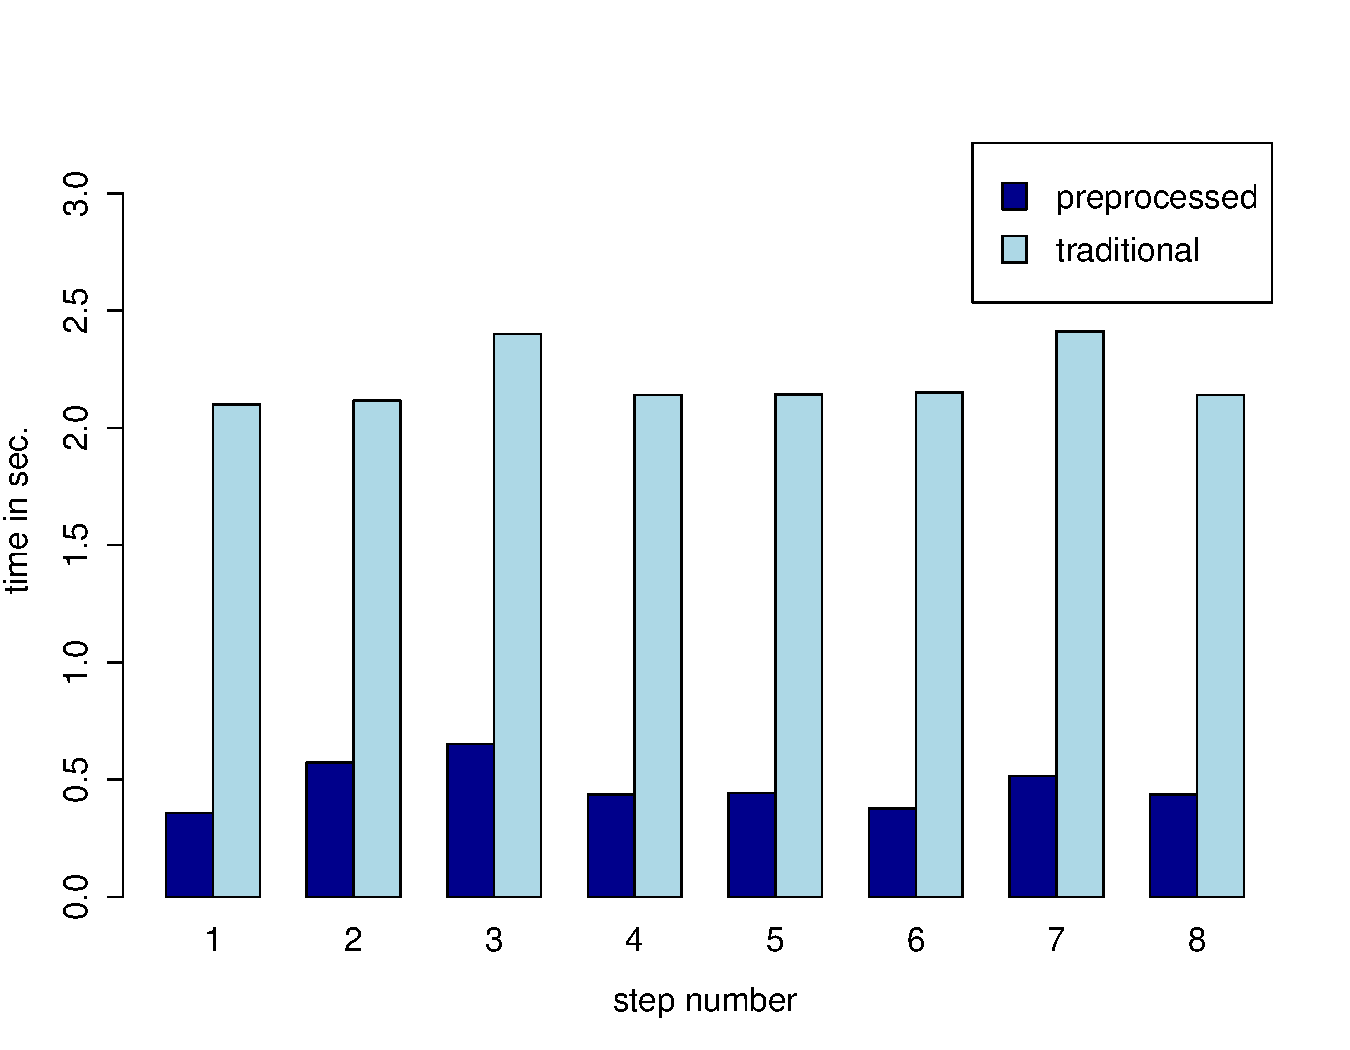
\includegraphics[width=0.5\textwidth]{Rplot26}
%     }
%   %  
%    % 
% %
% %
%     %}%\hfill
%     \subfloat[10 wards, reasoning time per event.\label{fig:results10ward}]{%
%       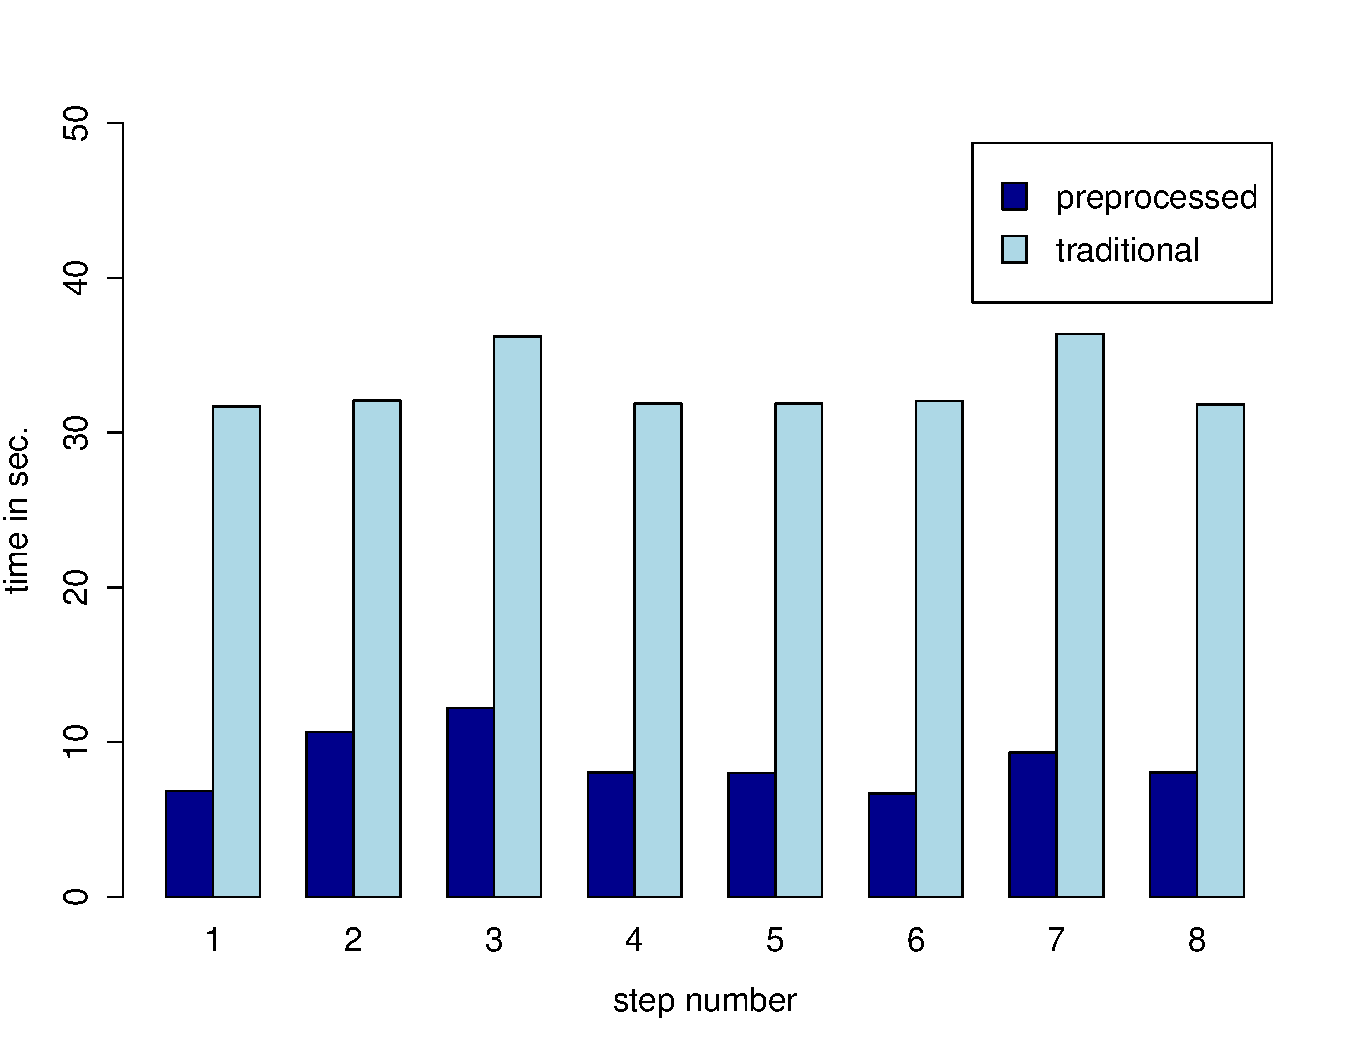
\includegraphics[width=0.5\textwidth]{Rplot27}
%     }
%     \caption{Comparison of reasoning times using preprocessed and traditional rules. The preprocessing step improves reasoning times.
%       }
%     \label{figure:results}
%   \end{figure}
%   
  
\begin{figure}
\centering
\begin{subfigure}{.5\textwidth}
  \centering
  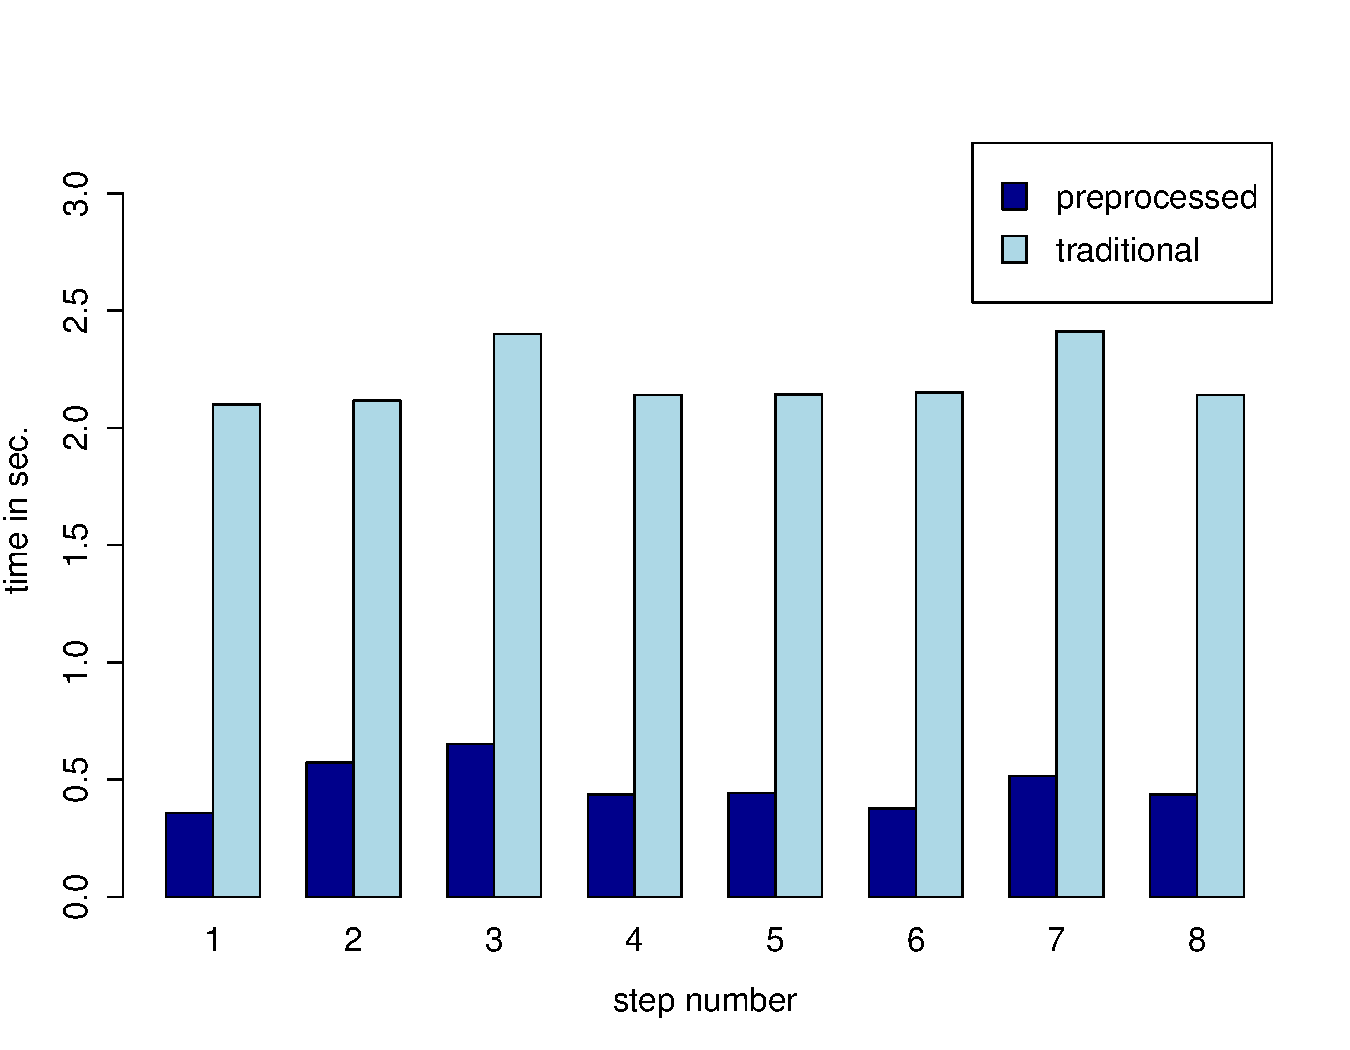
\includegraphics[width=\linewidth]{Rplot26}
  \caption{1 ward, reasoning time per event.}
  \label{fig:results1ward}
\end{subfigure}%
\begin{subfigure}{.5\textwidth}
  \centering
  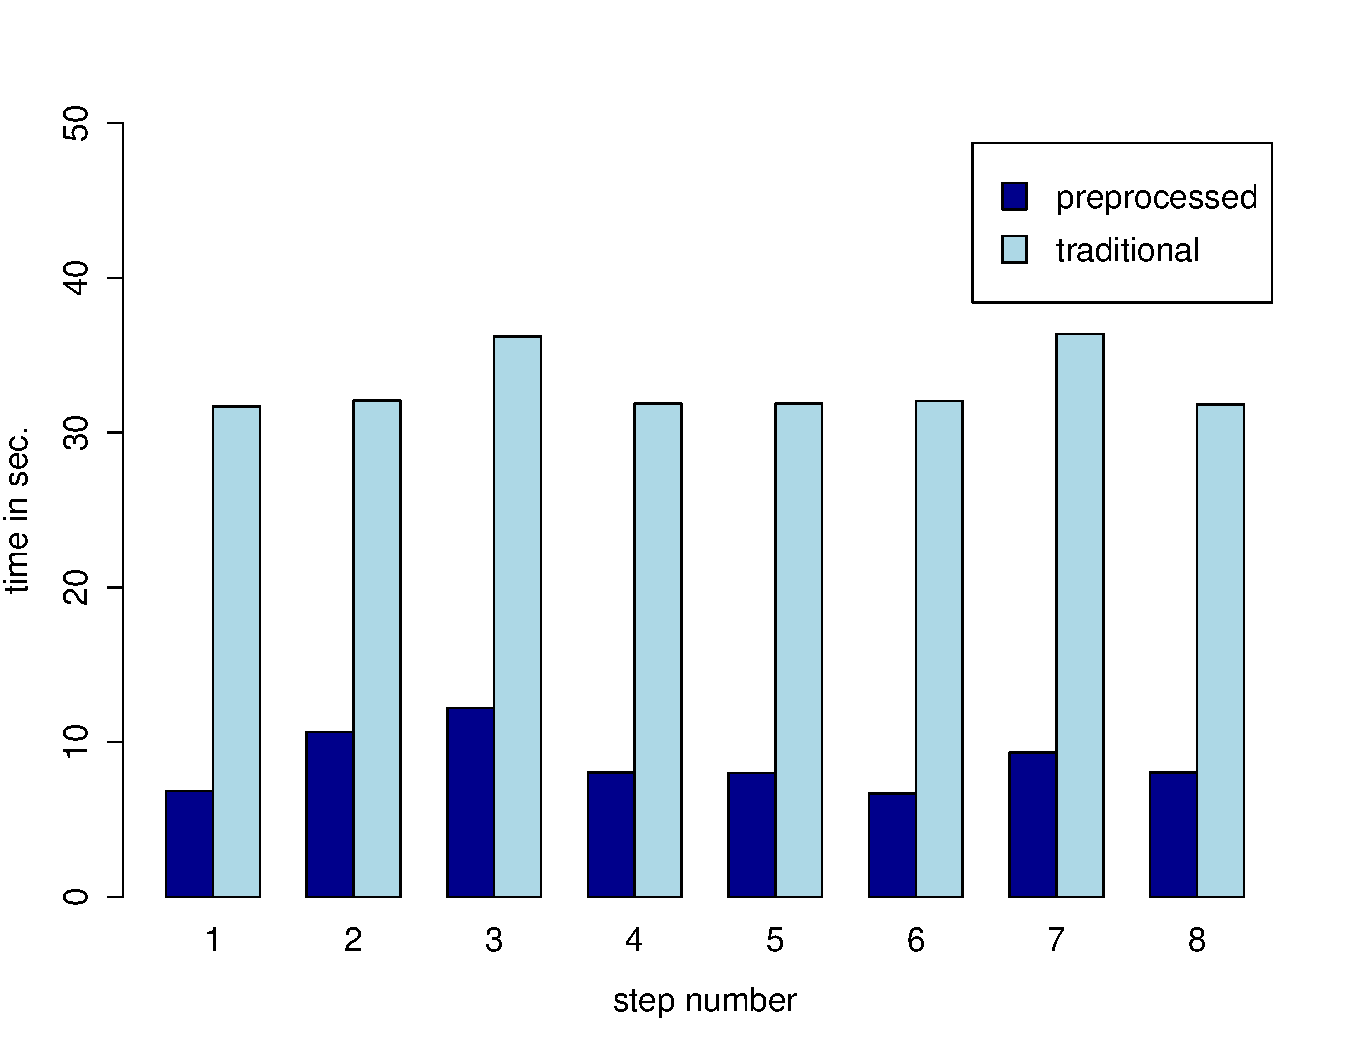
\includegraphics[width=\linewidth]{Rplot27}
  \caption{10 wards, reasoning time per event.}
  \label{fig:results10ward}
\end{subfigure}
\caption{Comparison of reasoning times using preprocessed and traditional rules. The preprocessing step improves reasoning times.}
\label{figure:results}
\end{figure} 
 

The figures show how preprocessing the rules improves reasoning times significantly,  consistently requiring only a quarter of the reasoning time.
This trend manifests itself regardless of the amount of dynamic data involved.
Whereas the traditional rule set can no longer be used in a hospital with 10 wards the 
preprocessed rule set still provides reasonable reasoning times. 
  

\subsection{Conclusion and Future Work}\label{conc}
In this paper we have shown that precomputing and using specialized rules based on the ontology's TBox improve reasoning times of OWL RL reasoning by about 75\%. 
The main cause
for that is that 
the newly computed rules are less complex---in terms of the variables which have to be unified during reasoning---than the
original version of the rules taken from the OWL RL 
profile description. 
Another aspect which makes reasoning faster in our set up is the fact that rules for concepts which are not even present in the ontology's TBox will not get 
produced by the preprocessing step. If for example the rather expensive concept \texttt{owl:sameAs} does not occur in any triple of the considered ontology,
no specialized rules will be produced for this concept.


The presented preprocessing step consists of two simple reasoning runs which can be performed before dealing with additional input data. Using the 
EYE reasoner this preprocessing normally takes only a few seconds. In set ups where the TBox does not change during run time the produced rules can be 
used whenever the ABox data to reason on changes as in the example introduced in this paper. Our approach is independent of the  reasoning done on top of the 
TBox by additional rules. This makes the rule version of the ontology's TBox even more suitable for reuse.


Our approach makes use of the special properties of Notation3 Logic.
By providing the option of using rules to produce new rules this logic is particularly suitable for our purposes. Furthermore Notation3 offers
multiple predicates to act on lists as for example the function \texttt{list:in}.
This eases the implementation of rule producing rules based on OWL predicates as there are many OWL constructs which are normally stated with lists 
in their object position.


Notation3 Logic posses other interesting properties which we are planning to apply in future work: in \nthree, rules can have existential variables in their 
consequence.
Using this particular property it will be possible to also cover OWL EL concepts which are not present in OWL RL. Similarly as done in 
for example OWLim \cite{elowlim} we are planning to include OWL EL in our implementation.  We furthermore want to investigate the actual costs of
processing the different OWL concepts by our newly produced rules. This will enable us to recommend the exclusion of particular concepts if not really needed. 


% $\forall x \exists $
% 
% \paragraph{\textbf{Acknowledgements}} The research activities described in this paper were funded by Ghent University, iMinds, the IWT Flanders, the FWO-Flanders, 
% and the European Union, in the context of the project ``ORCA'', which is a collaboration of Televic Healthcare, Internet-Based Communication Networks and Services (IBCN), and Multimedia Lab (MMLab).


% \FloatBarrier
% 
% 
% 
% \bibliographystyle{splncs03} 
% \bibliography{References} 
% 
% 
% 
% \end{document}


\section{Use Case: Data Validation}

\subsection{Introduction}

The amount of publicly available Linked Open Data (LOD) sets is constantly growing\footnote{See, eg statistics at: \url{http://lod-cloud.net/}.},
however, the diversity of the data employed in applications is mostly very limited:
only a handful of \rdf data is used frequently~\cite{rietveld2015lod}.
One of the reasons for this is that the datasets' quality and consistency varies significantly,
ranging from expensively curated to relatively low quality data~\cite{zaveri2015quality},
and thus need to be validated carefully before use.

One way to assess data quality is to check them against constraints: 
users can verify that certain data are fit for their use case,
if the data abide to their requirements.
First approaches to do that were implementations with hard coded validation rules,
such as Whoknows?~\cite{ketterl2011whoknows}.
Lately, attention has been drawn to formalizing RDF quality assessment, more specifically,
formalizing RDF constraints languages, such as Shape Expressions (ShEx)~\cite{shex} or Resource Shapes (ReSh)~\cite{resh}.
This detaches the specification of the constraints from its implementation.

Constraint languages allow users dealing with RDF data and vocabularies
to express, communicate, and test their particular expectations.
Such languages can either be (i) existing frameworks designed for different purposes, eg 
the query language SPARQL~\cite{hartmann2016,kontokostas2014test},
or the description logic based Web Ontology Language (OWL)~\cite{owlValidation},
or they can be (ii) languages only designed for validation, eg
ShEx~\cite{shex},
ReSh~\cite{resh},
Description Set Profiles (DSP)~\cite{dsp},
or the forthcoming \wwwc recommendation candidate Shapes Constraint Language (SHACL)~\cite{shacl}.
These different languages can be compared
by testing them on commonly supported constraints~\cite{bosch2015rdf,kontokostas2014test},
as conducted by Hartmann (n\'e Bosch) et al~\cite{bosch2015}.

Depending on the users' needs, constraint languages have to be able to cope with very diverse kinds of constraints which 
imply certain \emph{logical requirements}.
Such requirements were investigated by Hartmann et al~\cite{bosch2015} who
identified the Closed World Assumption (CWA) and the Unique Name Assumption (UNA) as crucial for validation. Since both are not 
supported by many Web Logics, Hartmann et al
 particularly emphasize
the difference between reasoning and validation languages
and favour SPARQL based approaches for validation
which -- if needed -- can be combined with OWL DL or QL reasoning.
In this paper, we take a closer look into these findings from a rule-based perspective:  
We show that neither UNA nor CWA are necessary for validation if a rule-based framework containing predicates 
to compare \uris and literals, and supporting
Scoped Negation as Failure (SNAF) is used. This enables us to --
instead of combining separate, successive systems --
do both \rdf validation \emph{and} reasoning in only one system which acts directly on a constraint language. 
We show the feasibility of this approach by providing an
implementation. 
This proof-of-concept is implemented in Notation3 Logic~(\nthreelogic)
and tackles the subset of the constraints
identified by Hartmann et al~\cite{bosch2015} 
which are covered in RDFUnit \cite{kontokostas2014test}.

The remainder of this paper is structured as follows:
In Section \ref{rw} we discuss related work.
In Section \ref{cons} we give an overview of common \rdf validation constraints.
In Section \ref{logic}, we discuss
how different requirements for \rdf validation are met by rule-based logics.
Section \ref{n3} explains the details of our proof of concept
and Section \ref{conc} concludes the paper and provides an outlook 
for future work.




\subsection{Related Work}\label{rw}

%intro
In this section, first,
we will present the state of the art around validation constraint languages.
Then, we will give an overview
of different languages and approaches used for \rdf validation.


%validation: constraints + reasoning
%\rdf validation in general and constraint types
Data quality can be described in many dimensions,
one of them being the intrinsic dimension, namely,
the adherence to a data schema~\cite{zaveri2015quality}.
In the case of \rdf data, this implies adhering to certain constraints.
These have been carefully investigated by several authors (eg Hartmann et al~\cite{hartmann2016}).
%Languages to express constraints
The formulation of (a subset of) these constraints can be done using existing languages (eg the Web Ontology Language (OWL)~\cite{owl}, 
the SPARQL Inferencing Notation (SPIN)~\cite{Knublauch2011}, or SPARQL~\cite{sparql})),
or via dedicated languages
(eg Shape Expressions (ShEx)~\cite{shex}, Resource Shapes (ReSh)~\cite{resh}, Description Set Profiles (DSP)~\cite{dsp}, 
or Shapes Constraint Language (SHACL)~\cite{shacl}.
Their execution is either based on reasoning frameworks, or querying frameworks.

On the one hand, Motik et al \cite{motik2007adding} and Sirin and Tau~\cite{sirin2009towards}
propose alternative semantics for OWL
which support the Closed World Assumption,
and are therefore more suited for constraint validation than the original version.
To know which semantics apply,
constraints have to be marked as such.
Using one standard to express both, validation and reasoning,
is a strong point of this approach,
however,  this leads to ambiguity: %as the exact same formula can have different meanings.
%
If the exact same formula can have different meanings, one of the key properties of the Semantics Web -- interoperability -- is in danger.
Another disadvantage of using (modified) OWL as a constraint language
is its limited expressiveness. 
Common constraints such as mathematical operations
or specific checks on language tags
are not covered by OWL~\cite{hartmann2016}.

On the other hand, SPARQL based querying frameworks for validation execution emerged (eg Hartmann \cite{hartmann2016} or Kontokostas et al \cite{kontokostas2014test}).
Where Hartmann proposes SPIN as base language to support validation constraints, Kontokostas introduces a similar but distinct language to SPIN,
more targeted to validation, so-called Data Quality Test Patterns (DQTP). 
DQTPs are generalized  SPARQL queries containing an extra type of variables. In an extra step, these variables are instantiated based on the  RDFS and OWL axioms used
by the data schema and can then be employed for querying. 
As such, the authors assume a closed world semantics for OWL
but in contrast to the approaches mentioned above,
this special semantics cannot be marked in the ontology itself.
They thus change the semantics of the common Web standard OWL.
To also find implicit constraint validation an extra reasoning step could be added,
but this step would then most probably assume the standard semantics of OWL,
further increasing the possibly of experiencing conflicts between the two contradicting versions of the semantics.
Hartmann proposes a dedicated ontology
to express integrity constraints, and as such,
this method does not involve changing existing semantics.
For both, involving reasoning is not possible without inclusion of a secondary system.



\subsection{\rdf Validation Constraints}\label{cons}


Based on the collaboration of
the W3C \rdf Data Shapes Working Group\footnote{\url{https://www.w3.org/2014/data-shapes/wiki/Main_Page}} and
the DCMI \rdf Application Profiles Task Group\footnote{\url{http://wiki.dublincore.org/index.php/RDF_Application_Profiles}}
with experts from industry, government, and academia,
a set of validation requirements has been defined,
based on which,
81 types of constraints were published,
each of them corresponding to at least one of the validation requirements~\cite{bosch2015rdf}.
This set thus gives a realistic and comprehensive view of what validation systems should support. 


Prior to this, the creators of RDFUnit~\cite{kontokostas2014test} had provided their own set of constraint types they support.
Given the usage of RDFUnit in real-world use cases~\cite{jurion_rdfunit},
this set gives a good overview
of what validation systems should minimally cover.


Table \ref{table:align} shows
the alignment of the 17 types of constraints as supported by RDFUnit
with the relevant constraint types as identified by Hartmann et al~\cite{bosch2015}. 
\sloppy
As can be seen, these types are not mapped one-to-one. 
One constraint from RDFUnit maps to
at least one constraint as identified by Hartmann, 
except for PVT and TRIPLE, which are both not very complex constraints and could thus easily be added to the work of Hartmann et al. 
In this paper, we mainly focus on these 17 constraints which are all covered by our implementation.
To make the topic of constraint validation more concrete, we discuss the examples (TYPEDEP), (INVFUNC) and (MATCH) in more detail  later in this paper 
and refer the interested reader to the above mentioned sources. 

\begin{table}
\caption{Constraints Alignment.
The first column lists the codes as used in RDFUnit;
the second column lists the constraints of Hartmann  following the numbering \cite[appendix]{hartmann2016}; and
the third column lists the description taken from RDFUnit.
}
\label{table:align}
\begin{tabular}{ p{0.2\textwidth} p{0.15\textwidth} p{0.65\textwidth}  } \toprule
\textbf{RDFUnit} & \textbf{Constraint Code} & \textbf{Description} \\ \midrule
 %\hline %\hline 
COMP & A11  &Comparison between two literal values of a resource\\ \midrule
%\hline
MATCH & A20, A21 &A resource's literal value (does not) matches a RegEx\\ \midrule
%\hline
LITRAN & A17, A18 &The literal value of a resource (having a certain type) must (not) be within a specific range\\ \midrule %\hline
TYPEDEP & A4 &Type dependency:  the type of a resource may imply the attribution of another type\\ \midrule %\hline
TYPRODEP & A41 &A resource of specific type should have a certain property\\ \midrule % \hline
PVT & B1 &If a resource has a certain value V assigned via a property P1 that in some way classifies this resource, one can assume the existence of another property P2\\ \midrule %\hline
TRIPLE & B2 &
A resource can be considered erroneous if
there are corresponding hints contained in
the dataset\\ \midrule %\hline
ONELANG & A28 &A literal value has at most one literal for a language\\ \midrule %\hline
RDFS-DOMAIN & A13 &The attribution of a resource's property
(with a certain value) is only valid if the
resource is of a certain type\\ \midrule % \hline
RDFS-RANGE & A14, A15 & The attribution of a resource's property is
only valid if the value is of a certain type\\ \midrule % \hline
RDFS-RANGED & A23 &
The attribution of a resource's property is
only valid if the literal value has a certain
datatype\\ \midrule %\hline
INVFUNC & A2 & Some values assigned to a resource are
considered to be unique for this particular
resource and must not occur in
connection with other resources\\ \midrule % \hline
OWL-CARD & A1, A32--37 & Cardinality restriction on a property\\ \midrule % \hline
OWLDISJC & A70 & Disjoint class constraint\\ \midrule % \hline
OWLDISJP & A69 & Disjoint property constraint\\ \midrule % \hline
OWL-ASYMP & A57 & Asymmetric property constraint\\ \midrule %\hline
OWL-IRREFL & A64 & Irreflexive property constraint \\ \bottomrule
\end{tabular}
\end{table}



\subsection{Features required for Validation}\label{logic}
After having listed the kind of constraints relevant for \rdf validation in the previous section, we will now focus on the suitability of rule-based logics for that task.
Based on the work of Sirin and Tao \cite{sirin2009towards}, and Hartmann et al \cite{bosch2015} who identified the logical requirements constraint 
languages need to fulfil,
we discuss why rule-based logic is a reasonable choice to validate \rdf datasets.




\subsubsection{Reasoning}\label{reasoning}
We start our discussion with reasoning. Hartmann \cite[p. 181]{hartmann2016} points out that performing reasoning in combination with \rdf validation brings several benefits:
constraint violations may be solved, violations which otherwise would stay undetected can be found, and datasets do not need to contain 
redundant data to be accepted by a validation engine. To better understand these benefits, consider the following ontology example:
\begin{equation}\label{subc}
 \texttt{:Reseacher rdfs:subClassOf :Person.}
\end{equation}
And the instance:
\begin{equation}\label{Kurt}
 \verb!:Kurt a :Researcher; :name "Kurt01".!
\end{equation}
If we now have a type dependency constraint (TYPEDEP) saying that every instance of the class \texttt{:Researcher} should also be an instance of the class \texttt{:Person}, 
which we test on the data above,
a constraint validation error would be raised since \texttt{:Kurt} is not declared as a \texttt{:Person}. If we perform the same constraint check after reasoning, the triple
\begin{equation}\label{person}
\verb!:Kurt a :Person.!
\end{equation}
would be derived and the constraint violation would be solved. Without the reasoning, Triple~\ref{person}
would need to be inserted into the dataset to solve the constraint,
leading to redundant data. 

To understand how reasoning 
can help to detect implicit constraints, consider another restriction: suppose that we have a constraint stating that a person's name should not contain 
numbers\footnote{This could be expressed by an extended version of MATCH as for example the constraint ``Negative Literal Pattern Matching'' in~\cite{hartmann2016}.}.
Without reasoning, no constraint validation would be detected because even though the \texttt{:name} of \texttt{:Kurt} contains numbers, \texttt{:Kurt} 
would not be detected as an instance of
\texttt{:Person}.


Hartmann's and many other validation approaches thus suggest to first perform a reasoning step and then do an extra validation step via SPARQL querying. 
The advantage of using rule-based reasoning instead is
that validation can take place during the reasoning process \emph{in one single step}. 
Relying on a rule which supports \texttt{rdfs:subClassOf} as for example presented 
in~\cite{arndt_ruleml_industry_2015}\todo{make reference to other chapter} the aforementioned problem could be detected.
In general, OWL-RL~\cite{OWLRL} can be applied since it is supported by every rule language.
If higher complexity is needed, rule languages with support for existential quantification can be used for OWL QL reasoning.


\subsubsection{Scoped Negation as Failure}
Another aspect which is important for constraint validation is negation.
Hartmann et al claim that the Closed World Assumption is needed to perform validation tasks.
Given that most Web logics assume the Open World Assumption, that would form a barrier for the goal of combining reasoning and validation 
mentioned in the previous section. Luckily, that is not the case.
As constraint validation copes with the local knowledge base,
Scoped Negation as Failure (SNAF), 
inter alia discussed in \cite{damasio2006supporting,kifer2005,polleres2006rules}, is enough.
Among the logics which support this concept are for example FLORA-2~\cite{negflora} or \nthreelogic~\cite{N3Logic}.

In order to understand the idea behind Scoped Negation as Failure,
consider the triples that form Formula~\ref{Kurt}
and suppose that these are the only triples in a 
knowledge base we want to validate. We now want to test the constraint from above that every individual which is declared as a researcher is also declared 
as a person (TYPEDEP). This means our system needs to give a warning if it finds an individual which is declared as a researcher, but not as a person:
\begin{multline}\label{constraint1}
 \forall \texttt{x}: ((\texttt{ x a :Researcher}) \wedge \neg (\texttt{ x a :Person}))\\ \rightarrow (\texttt{:constraint :is :violated.})
\end{multline}
In the form it is stated before, the constraint cannot be tested with the Open World Assumption. 
The knowledge base contains the triple 
\[\texttt{:Kurt a :Researcher.}\]
but not Triple~\ref{person},
but the rule is more general: given its open nature, 
we cannot guarantee that there is no document in the entire Web which declares Triple~\ref{person}.
This changes if we make an addition. Suppose that $\mathcal{K}$ is the
the set of triples
we can derive (either with or without reasoning) from our knowledge base consisting of Formula~\ref{Kurt}. Having $\mathcal{K}$ at our disposal, we can test:
\begin{multline}
 \forall \texttt{x}: ((\texttt{ x a :Researcher})\in \mathcal{K}) \wedge \neg ((\texttt{ x a :Person})\in \mathcal{K}))\\ \rightarrow (\texttt{:constraint :is :violated.})
\end{multline}
The second conjunct is not a simple negation, it is a negation with a certain scope, in this case $\mathcal{K}$. If we added new 
data to our knowledge like for example Triple~\ref{person}, we would have different knowledge $\mathcal{K}'$ for which other statements hold. The truth value of the formula above 
would not be touched since this formula explicitly mentions $\mathcal{K}$. The logic stays monotonic.
%Since we know all triples from $\mathcal{K}$, scoped negation is possible. 
Scoped negation as failure is the kind of negation we actually need in \rdf validation: we do not want to make and
test
statements in the Web in general, we just want to test the information contained in a local file or knowledge base.


\subsubsection{Predicates for Name Comparison}
Next to the Open World Assumption, 
Hartmann et al~\cite{bosch2015}
identify the fact that most Web logics do not base themselves on the Unique Names Assumption (UNA) 
as a barrier for them being used 
for constraint validation. This assumption is for example present in F-Logic \cite{flogic}  and basically states that every element in the domain of discourse
can only have one single name (\uri or Literal in our case).  The reason, why this assumption is in general problematic for the Semantic Web lies in its distributed nature: 
different datasets can -- and actually do -- use different names for the same individual or concept.
For instance, the \uri \texttt{dbpedia:London} refers to the same place in England as 
for example \texttt{dbpedia-nl:London}. In this case this fact is even stated in the corresponding ontologies using the predicate \texttt{owl:sameAs}.

The impact of the Unique Name Assumption for \rdf validation becomes clear if we take a closer look at OWL's inverse functional property and the related constraint (INVFUNC). 
Let us assume that \texttt{dbo:capital} is an \texttt{owl:InverseFunctionalProperty} and our knowledge base contains:
\begin{multline}\label{conflict}
 \texttt{:England dbo:capital :London. :Britain dbo:capital :London.}
\end{multline}
Since \texttt{:England} and \texttt{:Britain} are both stated as having \texttt{:London} as their capital and \texttt{dbo:capital} is an inverse functional property,
an OWL reasoner would derive  
\begin{equation}
 \texttt{:England  owl:sameAs :Britain.}
\end{equation}
Such a derivation cannot be made if the Unique Name Assumption is valid, since the former explicitly excludes this possibility. 

The constraint (INVFUNC) is related to the OWL concept above, but it is slightly different: while OWL's inverse functional property refers to the elements of the domain of
discourse denoted by the name, the validation constraint (INVFUNC) refers to the representation itself. Formula~\ref{conflict} thus violates the constraint. 
Even if our logic does not 
follow the Unique Name Assumption, this violation can be detected if the logic offers predicates to compare names.
In \nthreelogic,
\texttt{log:equalTo} and \texttt{log:notEqualTo}\footnote{\url{https://www.w3.org/2000/10/swap/doc/CwmBuiltins}.} are such predicates: in contrast to
\texttt{owl:sameAs} and \texttt{owl:differentFrom}, they do not compare the resources they denote, but their representation. 
The idea to support these kinds of
predicates is very common. So does, for example,
the Rule Interchange Format (RIF) cover several functions which can handle \uris and strings, 
as we will discuss in the next subsection.
 






\subsubsection{RIF Built-ins}\label{bisec}
In the previous subsection we indicated that a special predicate of a logic,
in this case \texttt{log:notEqualTo}, can be used to do \uri comparisons
and thereby support a concept which would otherwise be difficult to express. 
Such built-in functions are widely spread in rule-based logics
and play an important role in \rdf validation which very often deals with string comparisons, calculations or operations on \uri level.
While it normally depends on the designers of a logic which features are supported, there are also common standards. 

One of them is the Rule Interchange Format (RIF) \cite{rif}
whose aim it is to provide a formalism to exchange rules in the Web. 
Being the result of a \wwwc working group consisting of developers and users 
of different rule-based languages, RIF can also be understood as a reference for the most common features rule based logics might have. 
This makes the list of predicates~\cite{rifpredicates} supported by the different RIF dialects particularly interesting for our analysis. 
%\todo{AD: The next sentence is really loooong!}
And it is indeed the case that by
only using RIF predicates many of the constraints listed in Section \ref{cons} can already be checked: 
negative pattern matching (MATCH) can be implemented by using the predicate 
\texttt{pred:matches}, 
the handling of language tags as required for the constraint ONELANG can be done using \texttt{func:lang-from-PlainLiteral}, 
and for the comparison of literal values (COMP) there are several predicates to compare strings, numbers or dates.


To illustrate  how powerful RIF is when it comes to string validation, we take a closer look at the predicate \texttt{log:notEqualTo} from the previous section. 
In the example above it is used to compare two \uri representations and succeeds if these these two are different. To refer to a \uri value, RIF provides the predicate 
\texttt{pred:iri-string} which converts a \uri to a string and and vice versa. In \nthree notation\footnote{More about that in Section~\ref{n3syn}} 
that could be expressed by:
%\small
\begin{multline}
\texttt{(:England "http://exmpl.com/England") pred:iri-string true.}
\end{multline}
%\normalsize
To compare the newly generated strings, the function \texttt{func:compare} can be used. This function takes two string values as input,
and returns -1 if the first string 
is smaller
than the second one regarding a string order, 0 if the two strings are the same, and 1 if the second is smaller than the first. The example above gives:
\begin{multline}
 \texttt{("http://exmpl.com/Britain" "http://exmpl.com/England")}\\ \texttt{func:compare -1.}
\end{multline}
\sloppy
To enable a rule to detect whether the two \uri names are equal, one additional function is needed: the reasoner has to detect whether the result of the comparison
is not equal to zero. 
That can be checked using the predicate \texttt{pred:numeric-not-equal} which is the RIF version of $\neq$ for numeric values. In the present case the output 
of the comparison would be 
\texttt{true} since $0\neq 1$, a rule checking for the name equality of \texttt{:England} and \texttt{:Britain} using the three predicates would therefore be triggered.

Even though we needed three RIF predicates to express one \nthree predicate, the previous example showed how powerful built-ins in general -- but also the very common RIF predicates
in particular -- are. Whether a rule based Web logic is suited for \rdf validation highly depends on its built-ins. If it supports all RIF predicates, this can be seen as a strong
indication that it is expressive enough.


\subsection{Validation with \nthreelogic}\label{n3}
In the previous section we analysed the requirements
on a rule-based Web logic to be able to combine validation and reasoning:
it should support scoped 
negation as failure, it should provide predicates to compare different \uris and strings, and its built-in functions should be powerful enough to, inter alia, 
access language tags
and do string comparison as they are supported by RIF.
\nthreelogic as it is implemented in the EYE reasoner \cite{eyepaper} fulfils all these conditions. 
With that logic, we were able to implement rules for all the constraints listed in Section~\ref{cons}, and thus 
provide similar functionality as RDFUnit using rule-based Web logics.
Below we discuss the
details of this implementation starting by providing more information about \nthreelogic and EYE. 
The code of our implementation can be accessed at \url{https://github.com/IDLabResearch/data-validation}. 



\subsubsection{\nthreelogic}\label{n3syn}
\nthreelogic was introduced in 2008 by Tim Berners-Lee et al \cite{N3Logic} and is an extension of \rdf:
All \rdf turtle triples are also valid in \nthree. 
As in \rdf, blanknodes are understood as existentially quantified variables and the co-occurrence of two triples as in Formula~\ref{conflict} 
is understood as their conjunction. \nthree furthermore supports universally quantified variables. These are indicated by a leading question mark \texttt{?}. 
\begin{equation}
 \texttt{?x :likes :IceCream.}
\end{equation}
stands for \textit{``Everyone likes ice cream.''},  or in first order logic
\[\forall x: \text{likes}(x, \text{ice-cream})\]
Rules are written using curly brackets \texttt{\{~\}} and the implication symbol \texttt{=>}. The \texttt{rdfs:subClassOf} 
relation from Formula~\ref{subc} can be expressed as:
\begin{equation}\label{rulescl}
 \texttt{\{?x a :Researcher\} => \{?x a :Person\}.}
\end{equation}
Applied on Formula~\ref{Kurt} the rule results in Formula~\ref{person}. 
More details about syntax and semantics of \nthree can be found in our previous paper \cite{arndt_ruleml_2015}.

There are several reasoners supporting \nthree:
FuXi \cite{fuxi} is a forward-chaining production system for Notation3 whose reasoning is based on the RETE algorithm. 
The forward-chaining cwm \cite{cwm} reasoner 
is a general-purpose data processing tool which can be used for querying, checking, transforming 
and filtering information.
EYE \cite{eyepaper} is a reasoner enhanced with Euler path detection. 
It supports 
backward and 
forward 
reasoning and also a user-defined mixture of both. 
Amongst its 
numerous features are the option to skolemise blank nodes
and  the possibility to produce and reuse proofs for further reasoning. 
The reason why we use EYE in our implementation is its generous support for built-ins\footnote{\url{http://eulersharp.sourceforge.net/2003/03swap/eye-builtins.html}}: 
next to \nthree's native built-ins\footnote{\url{https://www.w3.org/2000/10/swap/doc/CwmBuiltins}}, 
RIF, but also several other functions and concepts are implemented. 


\subsubsection{Expressing Constraints}


\begin{lstlisting}[
  float=t,
  caption={Example inverse functional property constraint: No city can be the capital of two countries. },
  label=example2]
§\textcolor{gray}{@prefix rdfcv: \url{<http://www.dr-thomashartmann.de/phd-thesis/rdf-validation/vocabularies/rdf-constraints-vocabulary\#>}.}§
§\textcolor{gray}{@prefix : <http://example.com/constraints\#>.}§
§\textcolor{gray}{@prefix dbo: 	<http://dbpedia.org/ontology/> .}§

:example_constraint a rdfcv:SimpleConstraint ;
  :constraintType :InverseFunctionalProperties ;
  rdfcv:constrainingElement :inverse-functional-properties ;
  rdfcv:leftProperties ( dbo:capital ) ;
  rdfcv:contextClass  dbo:Country .
\end{lstlisting}

Before we can detect violations of constraints using \nthree logic,
these constraints first need to be stated.
This could either be done by directly expressing them in 
rules -- and thereby creating
a new constraint language next to the ones presented in Section~\ref{rw} -- or on top of existing \rdf-based conventions. 
%The first option would require a certain level of knowledge of \nthree and its builtins---for example \nthree's way to express scoped negation as failure---
%While the first option would require a deeper knowledge of \nthree and its built-in functions, the second option just expects the user to know \rdf and  
We opt for the latter and base our present implementation on the work of Hartmann \cite[p.167 ff]{hartmann2016}:
in his PhD thesis, Hartmann presents a lightweight vocabulary to describe any constraint, 
the RDF Constraints Vocabulary (RDF-CV)\footnote{\url{https://github.com/boschthomas/RDF-Constraints-Vocabulary}}. The reason why we chose that vocabulary over 
the upcoming standard
SHACL is its expressiveness. We aim to tackle the 81 constraints identified by Hartmann which are not all expressible in SHACL 
or any other of the constraint languages
mentioned in Section~\ref{rw} \cite[p.52, appendix]{hartmann2016}. As will be shown in the following section, it is not difficult to adopt the rules to different 
constraint languages as long as they are based on \rdf and as such valid \nthree expressions.

RDF-CV supports the concept of so called \emph{simple constraints} which are all the constraints expressible by the means of the vocabulary, in particular 
the ones mentioned in Section~\ref{cons}. Each simple constraint has a constraining element. Where applicable, the names of these elements are inspired by their related 
DL names, but the constraining element can also be for example the name of a SPARQL function. In some cases, the same constraint type 
can be marked by different constraining elements as for example the constraint COMP whose constraining element is the relation 
used to compare values 
(eg the usual numerical orders: $<,>,\leq$, and $\geq$) or there can be different constraint types sharing the same constraining element.
To be sure that cases like this do not cause any ambiguity we additionally assign a \emph{constraint type} to every constraint. 
The names of these types follow the names used by Hartmann~\cite[appendix]{hartmann2016}. 
The TYPEDEP constraint from Section~\ref{reasoning} is for example of constraint type \texttt{:Subsumption}.

In addition to constraining element and constraint type, there are several predicates to assign the constraints to individuals and classes: \emph{context class}, 
\emph{classes}, 
\emph{leftProperties}, 
\emph{rightProperties}, and \emph{constraining values}.
The \emph{context class} of a constraint fixes the set of individuals for which a constraint must hold. For the subsumption constraint mentioned above, that would be 
the class \texttt{:Researcher}, the constraint talks about \emph{every} individual labelled as \emph{researcher}. 
There could be other classes involved. In our subsumption example that is the superclass the  
individuals should belong to, \texttt{:Person}. Every researcher should also be labelled as \emph{person}. %The whole subsumption example is displayed in Listing~\ref{subcc}. 
Since these kinds of properties can be multiple, 
they are given in a
list. How and if the predicate  \emph{classes} is used depends on the constraint.
The predicates \emph{leftProperties} and \emph{rightProperties} are used to do similar statements about properties. The constraint INVFUNC as displayed in 
Listing~\ref{example2} makes for example use of it to 
relate the constraint specified to the predicate it is valid for. The objects of the predicates \emph{leftProperties} and \emph{rightProperties} are lists. The predicate 
\emph{constraining value}
 is used for the predicates where a literal value is needed to further specify a constraint. An example for such a constraint is MATCH as described in Section~\ref{reasoning}. To 
 express, that a name should not contain numbers, the predicate \emph{constraining value} connects the constraint to the string pattern,
 \texttt{"[1-9]"} in the present case. 



\subsubsection{Constraint Rules}\label{rules}
\begin{lstlisting}[
  float=t,
  caption={Rule for inverse functional property (INVFUNC). The predicate \texttt{log:notEqualTo} compares the resources based on their URI and thereby supports 
  the Unique Name Assumption. },
  label=invfunc]
§\textcolor{gray}{@prefix rdfcv: \url{<http://www.dr-thomashartmann.de/phd-thesis/rdf-validation/vocabularies/rdf-constraints-vocabulary\#>} .}§
§\textcolor{gray}{@prefix : <http://example.com/constraints\#> .}§
§\textcolor{gray}{@prefix list: <http://www.w3.org/2000/10/swap/list\#>.}§
§\textcolor{gray}{@prefix log: <http://www.w3.org/2000/10/swap/log\#> .}§

{
?constraint a rdfcv:SimpleConstraint;
  :constraintType :InverseFunctionalProperties;
  rdfcv:constrainingElement :inverse-functional-properties;
  rdfcv:leftProperties ?list;
  rdfcv:contextClass  ?Class.
  
?object a ?Class.
?property list:in ?list.
?x1 ?property ?object.
?x2 ?property ?object.
?x1 log:notEqualTo ?x2
}
=>
{
[] a :constraintViolation;
    :violatedConstraint ?constraint.
}.
\end{lstlisting}


Having seen in the last section one possible way to describe constraints on \rdf datasets, this section explains how these descriptions can be used. We employ rules
which take the expressed constraints and the \rdf dataset to be tested into account and generate triples indicating constraint validations, if present. 
We illustrate that by an example: In  Listing~\ref{invfunc} we provide a rule handling the constraint INVFUNC. Lines 7--11 contain the details of the constraint. The rule
applies for simple constraints of the type \emph{inverse functional properties} for which a context class \texttt{?Class} and a list \texttt{?list} of left properties 
is specified.
This part of the rule's antecedence unifies with the constraint given in Listing \ref{example2}. Lines 13--18 describe which situation in the tested data causes 
a constraint violation: for an \texttt{?object} which is an instance of \texttt{?Class}, there are two subjects, \texttt{?x1} and \texttt{?x2}, defined 
which are both connected 
to \texttt{?object} via \texttt{?property}. This \texttt{?property} is an element of \texttt{?list},
and the names, ie the \uri- or string-representations, of \texttt{?x1} and \texttt{?x} differ. The latter is expressed using the predicate
\texttt{log:notEqualTo}\footnote{As explained in Section~\ref{bisec} 
there are alternative ways to express the predicate \texttt{log:notEqualTo} in \nthree, the antecedence of the entire rule could also be expressed only using RIF predicates.} 
(Line 18). Together with Listing~\ref{example2} that violation is thus detected if two different resource names 
for resources of the class \texttt{dbo:Country} are connected via the predicate \texttt{dbo:capital} to the same object. Assuming that \texttt{:Britain} and \texttt{:England}
are both instances of the class \texttt{dbo:Country}, the triples in Formula~\ref{conflict} lead to the violation:
\begin{equation}
 \texttt{\_:x a :violaton; :violatedConstraint :example\_constraint.}
\end{equation}
The example shown relies on descriptions following the vocabulary Hartmann suggests, but our approach can easily be adapted for 
other \rdf based constraint vocabularies. All  we need is a consistent way to express constraints in \rdf. 
Note that our rules act directly on constraint descriptions and \rdf datasets: while the SPARQL based approaches \cite{hartmann2016,kontokostas2014test} mentioned 
in Section~\ref{rw} rely on an extra mapping step
to instantiate the search patterns. If reasoning needs to be included into the data validation, a rule based system can do reasoning, mapping and constraint validation 
in one single step  where other systems need to perform three.


\subsection{Conclusion and Future Work}\label{conc}
In this paper we investigated the requirements a rule based Web logic needs to fulfil to be suitable for \rdf validation:
it should support Scoped Negation as Failure, it should provide predicates for name comparison, and its built-ins should be powerful enough to, for example, 
do string comparisons or access language tags.  Together with the capability to meet its primary purpose, Web reasoning, such a Web logic is
a strong alternative to the common approach of either combining reasoning and validation in two different steps, for example by first performing OWL reasoning and 
then executing SPARQL queries on top of the result as done by Hartmann \cite{hartmann2016}, or only executing SPARQL queries and thereby ignoring possible 
implicit constraint violations
as done in RDFUnit~\cite{kontokostas2014test}. Rule based Web logics fulfilling the requirements still provide the same expressivity as SPARQL with the additional advantage
of supporting reasoning. Validation and reasoning can thus be done by \emph{one single system} in \emph{one single step}. 
%
The practical feasibility of this approach has been shown by providing a proof-of-concept in \nthreelogic which supports all RDFUnit constraint types. 
As such, we allow users to assess 
their data quality more easily using a single rule based validation system, and potentially uncovering more errors. Thus, improving data quality on the Semantic Web overall.

In future work, we are planning to extend our implementation:
we aim to cover all of the 81 constraints identified by Hartmann et al \cite{bosch2015} which are not specific to SPARQL. We furthermore 
envisage to extend the supported \rdf constraint vocabularies and to align our efforts with SHACL.  
Another direction of future research will be a better combination of performant reasoning and validation, following the ideas provided in previous work~\cite{arndt_owled_2015}.
Further evaluation on performance is also to be conducted.

\todo{add evaluation results from Ben's paper}
%\section{Use case: Data Validation}
\label{validation}


\section{Conclusion}
In order to answer the question whether \nthreelogic can solve the same practical problems as SPARQL and OWL DL reasoning with a comparable performance we considered two use cases:
A semantic nurse call system and a system for \rdf validation.  

The nurse call system has been previously implemented using OWL DL reasoning to draw conclusions from the ontology involved
and SPARQL querying to select a nurse based on the reasoning 
result. 
We implemented a system which combined ontology reasoning and querying using only one framework: \nthreelogic. To draw conclusions from 
the knowledge expressed in the ontology, we applied OWL RL reasoning. 
% While this was enough for our use case, such rules 
% making sense of the concepts used in OWL ontologies could be further extended if needed. 
The decision tree
for assigning nurses to a call depending on the current context has been implemented by directly using \nthree rules. 
We compared the execution times of both implementations and saw that the solution using \nthree performed faster which was caused by two reasons:
Firstly, we only took the \owl concepts which were relevant for our use case into account and not all inference steps included in the profile OWL DL. 
This optimisation could be made because \nthreelogic is very flexible: using rules we can choose which OWL concepts we want to support. 
Since \nthree also supports existential rules and is in most reasoners enriched with various built-ins, we can go beyond OWL RL if needed 
(see also Section~\ref{owln3} below).
The second reason for the good performance was that two different tasks -- querying and ontology reasoning -- could be performed by one single framework and
not by two 
different ones as in the original implementation. Here, \nthree completes the task of a \emph{unifying logic} and connected the building blocks \emph{Querying} and 
\emph{Ontologies/Taxonomies}.

For the second use case  we considered -- \rdf data validation -- SPARQL is normally seen as the method of choice~\cite[p. 143]{hartmann2016}. By implementing 
rules for the constraint types supported by RDFUnit -- a very popular engine to test constraints on \rdf datasets -- 
we showed that this typical use case for querying 
can also be supported by \nthreelogic. The comparison of our implementation with RDFUnit showed that both implementations are comparable in terms of accuracy and 
execution times. For small datasets our implementation was faster, for datasets containing more than 100,000 triples RDFUnit performed better.
The real advantage of using \nthree reasoning instead of SPARQL querying was in this case again the fact that our system can be easily extended to perform more complex 
reasoning.

Both use cases we considered were originally approached using OWL DL reasoning and/or SPARQL querying and we could retrieve 
comparable -- and in some aspects even better -- results by applying 
\nthreelogic instead. This indicates that \nthreelogic -- if equipped with the right set of built-in predicates -- can connect the layers \emph{Querying}
and \emph{Ontologies/Taxonomies} for the Semantic Web stack just as we expect it from a \emph{Unifying Logic}.




\newpage
This chapter was partly based on the publications:
\vspace{0.3cm}

\bibentry{arndt_ruleml_industry_2015}

\vspace{0.3cm}

\bibentry{arndt_owled_2015}

\vspace{0.3cm}

\bibentry{arndt_rulemlrr_2017}

\vspace{0.3cm}

\bibentry{ben}

\chapter{Proofs in N3}\label{proof}
%\section{A Proof Calculus for N3}
By now, we have discussed three of the four characteristics we identified as crucial for a \emph{Unifying Logic} for the Semantic Web (Section~\ref{req}): 
A clearly defined semantics, 
syntactic and semantic compatibility with \rdf, and the power to connect the logical building blocks \emph{Querying}, \emph{Ontologies/Taxonomies} and \emph{Rules}. 
The fourth aspect in this list, the support of the layer \emph{Proof}, is the topic of the following two chapters. It should be possible to express and exchange proofs
 by making use of the \emph{Unifying Logic}. % of the Semantic Web should support proofs:
% It needs to be possible 
% to express proofs in that logic in 
These proofs should not only support the layer of \emph{Trust} but should also be suitable to be used in practical applications.  

We discuss the relationship of \nthreelogic and the layer of \emph{Proofs} in two steps: Firstly, 
we further elaborate in this chapter on the SWAP~\cite{SWAP} proof vocabulary\footnote{\url{http://www.w3.org/2000/10/swap/reason\#}} 
which we already briefly discussed in Section~\ref{proofintro}. 
We formally define the calculus it expresses and prove its correctness. 
In the following chapter we will then take a closer look to the practical applications of proofs: next to establishing 
trust, proofs can, for example, also be used to do planning or to identify the potentially critical streams in a bigger set-up of streaming sensors. 
%Below, we explain these two use cases in more detail.
% vocabulary
% introduced in the context of the Semantic Web Application Platform (SWAP)~\cite{SWAP}

% In the previous chapters we discussed how the semantics of \nthreelogic can be defined, its relation to \rdf and its ability to connect the logical building blocks
% of the Semantic Web Layer cake. 
% Having dons that, we covered three of the four requirements we had on a unifying logic 
% As discussed in Section~\ref{req}, all these aspects are crucial for a logic to become the unifying logic of the Semantic Web.
% we identified all these aspects as crucial properties for a \emph{Unifying logic} for the Semantic Web but there 
% was one more relevant aspect for such a logic: it should support the \emph{Proof} layer. 

\section{The direct semantics of N3}
%\section{A proof calculus for N3}
\label{nthree}
We start this chapter with formal considerations: To be able to discuss about the possible applications of proofs in \nthree, we first need to 
clarify the calculus behind it and -- most important -- prove its correctness based on the semantics of \nthree. We already know, 
that this semantics of \nthree is 
rather problematic: In Section~\ref{semofn3} we formalised two possible alternatives to understand the meaning of nested implicitly universally quantified variables
and it is very likely, that there are even more ways to understand implicit quantification in \nthree. 
%Even though we stated our own preferences, we  rather would like this matter to be discussed in the community instead of making a concrete choice here. 
Since we want to keep our findings valid for all implementations -- proofs should 
be exchangeable among the different reasoners -- we limit our considerations about the proof calculus to those formulas whose implicitly universally
quantified variables are not ambiguous. These are the formulas in which such variables do not occur in deeply nested expressions. We call such formulas \emph{simple formulas}. 
Below, we define the semantics of such formulas. %\todo{here or somewhere else: why are we not using the elaboration semantics?}
Opposed to the previous chapters, we will use a direct approach here, mainly because this makes the later proofs concerning the proof calculus easier to follow. 
 



%\subsection{Semantics of simple formulas}
In our previous examples, implicit universal quantification in \nthree always lead to a problem when it occurred deeply nested in a formula. While example 
Formula~\ref{uni} from Section~\ref{vars}
\begin{multline}\notag
 \texttt{\{:Kurt :knows ?x.\} => }%} \\ \texttt{
 \texttt{\{?x :knows :Kurt.\}.}%\nonumber
\end{multline}
had a clear meaning in both interpretations, namely
\[
 \forall \texttt{x}: \texttt{<Kurt knows x>}\rightarrow \texttt{<x knows Kurt>}
\]
we had two conflicting interpretations for Formula~\ref{fff}:
\begin{multline}\notag
\texttt{\{\{?x :q ?y.\} => \{?x :r :c.\}.\} =>}
\texttt{\{?x :p :a.\}.}
\end{multline}
The problem with that last formula was that Cwm and EYE differ in their understanding of the concept \emph{parent}  
for universal variables which only occur nested -- ie surrounded by at least two pairs of curly brackets \texttt{\{~\}} -- in a formula.  Here, that is the case 
for the universal variable
\texttt{?y}. For Cwm, the next higher formula surrounded by curly brackets is the parent, it carries the quantifier -- that is the formula \texttt{\{?x :q ?y.\} => \{?x :r :c.\}.} in the example --
while for EYE the top formula is always the parent. \emph{Simple formulas} are now the formulas where universal variables do not occur nested 
and which are therefore interpreted 
equally by both reasoners. 

In order to formally define \emph{simple formulas}, we first introduce the concept of nested components.
The definitions that follow rely on the syntax definitions we gave in Section~\ref{n3synsec}, in particular the \nthree alphabet (Definition~\ref{alphabet}) 
and the grammar given in 
Figure~\ref{N3S}. 
%These definitions state how terms and expressions can be constructed and how these can be composed to formulas. We had three different kinds of formulas:
% As we are going to use this terminology below, we repeat here the three different kinds of formulas we had:
% \begin{enumerate}
%  \item \emph{atomic formulas} \texttt{t t t.} consisting of three terms,
%  \item \emph{implications} \texttt{e => e.} where \texttt{e} are expressions, and
%  \item \emph{conjunctions} \texttt{f f} consisting of two formulas.
% \end{enumerate}
%
% %\todo{cite \cite{semN3}}
% 
% %\todo{Plan: stay with my formalisation (improves version), then limit to nesting level 2 and say that we have existential rules. Maybe cite a nice paper aboout existential rules.
% %What do you think Ruben?}
% \restdesc descriptions are expressed in the Notation3 (\nthree) rule language~\cite{N3Logic,Notation3}.
% We will introduce the \nthree language and its logic,
% focusing on the aspects relevant to our purposes. Our formalization is based on the formalization we gave in a previous paper \cite{semN3} and the informal
% semantic descriptions given in the above mentioned sources.
% %F\todo{cite \cite{semN3}}
% %\todo{Stay with the new formalisation of use simple FOL in the first place?}
% %%%%%%%%%%%%%%%%%%%%%%%%%%%%%%%%%%%%%%%%%%%%%%%%%%%%%%%%%%%%%%%%%%%%%%%%%%%%%%%%%%%%%%%%%%%%%%%%%%%%%%%%%%%%
% % Syntax
% %%%%%%%%%%%%%%%%%%%%%%%%%%%%%%%%%%%%%%%%%%%%%%%%%%%%%%%%%%%%%%%%%%%%%%%%%%%%%%%%%%%%%%%%%%%%%%%%%%%%%%%%%%%%
% \nthree augments the RDF model with symbols for quantification, implication, and statements about formulas:
% 
% 
% \begin{definition}[Basic N3 vocabulary]
% An \emph{N3 alphabet~$A$} consists of the following disjoint classes of symbols:
% \begin{itemize}
% \item A set $U$ of \uri symbols.
% \item A set $V=V_E\mathbin{\dot{\cup}} V_U$  of (quantified) variables, with $V_E$ being the set of existential variables
% and $V_U$ the set of universal variables.
% \item A set $L$  of literals.
% \item A boolean literal \verb!false!
% \item Brackets \verb!{!, \verb!}!, \verb!(!, \verb!)!
% \item Logical implication $\verb!=>!$ 
% \item Period \verb!.!
% \end{itemize}
% \end{definition}
%
% 
% 
% We define the elements of $U$ as in the corresponding specification~\cite{iri}.
% \nthree allows to abbreviate URLs as prefixed names~\cite{turtle}.
% Literals are strings beginning and ending with quotation marks `\verb!"!';
% existentials start with `\verb!_:!', universals with `\verb!?!'.
% 
% \nthree does not distinguish between predicates and constants---%
% a single \uri symbol can stand for both at the same time---%
% so the first-order-concept of a~\emph{term}
% has a~slightly different counterpart in \nthree: an \emph{expression}.
% Since the definition of expressions (Definition~\ref{expression})
% is closely related to the concept of a~formula (Definition~\ref{formula}),
% the two following definitions should be considered together.
% 
% \begin{definition}[Expressions]\label{expression}
%   Let $A$ be an \nthree alphabet.
%   The set of \textit{expressions} $E \subset A^{*}$ is
%   defined as follows:
%   \begin{enumerate}
%     \item Each \uri is an expression.
%     \item Each variable is an expression.
%     \item Each literal is an expression.
%     \item \label{list} If $e_1,\ldots,e_n$ are expressions, $\verb!(!e_1 \ldots e_n\verb!)!$ is an expression. 
%     \item \label{false} \verb!false! is an expression.
%     \item $\verb!{ }!$ is an expression.
%     \item \label{fe} If $f\in F$ is a formula, then $\verb!{!f\verb!}!$ is an expression. 
%   \end{enumerate}
%   The expression defined by \ref{list} is called a \textit{list}.
%   We call the expressions defined by \ref{false}--\ref{fe}
%   \textit{formula expressions} and denote the set of all formula expressions by $\mbox{\textit{FE}}$.
% \end{definition}
%
%
% Note that point \ref{fe} of the definition above makes use of formulas, which are defined as follows:
% 
% \begin{definition}[\nthree Formulas]
%     \label{formula}
%     The set~$F$ of \textit{\nthree formulas} over alphabet~$A$ is recursively defined as follows:
%     \begin{enumerate}  
%       \item \label{1} If $e_1, e_2, e_3 \in E$, then the following is a formula, called \textit{atomic} formula: \[e_1~ e_2~ e_3.\] 
%       \item \label{2} If $t_1, t_2$ are formula expressions then the following is a formula, called \mbox{\textit{implication}}: \[t_{1} \verb!=>!~t_{2}.\] 
%       \item \label{n} If $f_1$ and $f_2$ are formulas, then the following is a formula, called \textit{conjunction}: \[f_1 f_2\] 
%     %  \item Nothing else is a formula.
%     \end{enumerate}
% \end{definition}
% 
% We will refer to a~formula without any variables as a~\textit{ground formula}.
% Analogously, we call expressions without any variables \textit{ground expressions}.
% We denote the corresponding sets by $F_g$ respectively $E_g$. 
% An formula or expression which does not contain universal variables is called \emph{universal free}. 
% The set of universal free formulas (possibly containing existentials) is denoted by $F_e$, the set of universal free expressions by $E_e$.
% 
% In the examples in the remainder of this paper, we will use the common \rdf shortcuts:
% 
% \begin{remark}[Syntactic variants]
% \begin{itemize}
% \item A formula consisting of two triple subformulas starting with the same element \verb!<d> <p> <e>. <d> <q> <f>.! can be abbreviated using a semicolon: \verb!<d> <p> <e>; <q> <f>.!\\ 
% Two triple formulas sharing the first two elements  \verb!<d> <p> <e>. <d> <p> <f>.! can be abbreviated using a comma: \verb!<d> <p> <e>, <f>.!
%   \item \verb![]! can be used as an expression and is a shortcut for a new existential variable. So \verb![] <p> <d>.! stands for \verb!_:x <p> <d>.!
%   %If $[~]$ occurs in a formula $f$ instead of an expression, each instance of $[~]$  can be translated by a new existential variable.
%  \item An expression of the form \verb![<p> <o>]! is a shortcut for a new existential variable \verb!_:x!,
%    which is subject to the statement \verb!_:x <p> <o>.!
%    So \verb! <s> <p> [<q> <o>].! stands for \verb!<s> <p> _:x. _:x <q> <o>.!
%  \item \verb!a! is a~shortcut for \verb!rdf:type!~\cite{RDF}.
%  \end{itemize}
% \end{remark}
% 
In the definitions and examples which follow we will make use of the brackets occurring in \nthree's syntax \texttt{\{}, \texttt{\}}, \texttt{(}, \texttt{)} and of auxiliary 
brackets we use in mathematical expressions.
 To emphasize the difference between these two kinds of brackets,
%  brackets which form part of the \nthree vocabulary, i.e. ``\verb!(!'', ``\verb!)!'', ``\verb!{!'', and ``\verb!}!'', 
%  and the brackets occurring in mathematical language,
 we will underline the \nthree brackets in all definitions where both kinds of brackets occur.
% 
% 
%%%%%%%%%%%%%%%%%%%%%%%%%%%%%%%%%%%%%%%%%%%%%%%%%%%%%%%%%%%%%%%%%%%%%%%%%%%%%%%%%%%%%%%%%%%%%%%%%%%%%%%%%%%%%%%%%%%%%%%%%%%%%%%%%%%%%%%%%
%Semantics
% %%%%%%%%%%%%%%%%%%%%%%%%%%%%%%%%%%%%%%%%%%%%%%%%%%%%%%%%%%%%%%%%%%%%%%%%%%%%%%%%%%%%%%%%%%%%%%%%%%%%%%%%%%%%%%%%%%%%%%%%%%%%%%%%%%%%%%%%%
% As in \rdf, s
% Simple N3 triples of the form \verb!:s :p :o! can be understood as a first order formula $p(s,o)$. We call \texttt{:p} the predicate, \texttt{:s} 
%  the subject and \texttt{:o} the object of a triple. More complicated constructs often contain variables:
% in Notation3 existential and universal variables %occurring in formulas 
% are implicitly quantified. 
Using that notation, we define:
% The scope of this quantification depends on how deeply nested
% a variable occurs in a formula. To be able to make statements about that we define:



\begin{definition}[Components of a formula]
Given an \nthree alphabet $\mathcal{A}$.
Let $\mathcal{F}$ be the set of \nthree formulas and $\mathcal{T}$ 
the set of terms over $\mathcal{A}$. Let $f\in \mathcal{F}$ be a formula and $c:\mathcal{T} \rightarrow 2^\mathcal{T}$ a~function such that:
\[c(e)=\begin{cases}
  
  c(e_1)\cup\ldots\cup c(e_n) & \text{if }e=\underline{\texttt{(}}e_1 \ldots e_n\underline{\texttt{)}}\text{ is a list,}\\
  \{e\}  & \text{otherwise.}
\end{cases}\]



We define the set $\textit{comp}(f)\subset \mathcal{T}$ of \emph{direct components} of $f$ as follows:
 \begin{itemize}
  \item If $f$ is an atomic formula of the form $t_1~ t_2~ t_3.$, $\textit{comp}(f)=c(t_1)\cup c(t_2)\cup c(t_3)$.
  \item If $f$ is an implication of the form $e_{1} \verb!=>!~e_{2}.$, then $\textit{comp}(f)=\{e_1, e_2\}$.
  \item If $f$ is a conjunction of the form $f_1 f_2$, then $\textit{comp}(f)=\textit{comp}(f_1)\cup \textit{comp}(f_2)$.
 \end{itemize}
 Likewise, for $n\in \mathbb{N}_{>0}$, we define the \emph{components of level $n$} as:
 \begin{flalign*} 
  \textit{comp}^n(f):= &  
  \{t\in \mathcal{T}|\exists f_1,\ldots, f_{n-1}\in \mathcal{F}: 
   t\in \textit{comp}(f_1)\wedge  \underline{\texttt{\{}}f_1\underline{\texttt{\}}}\in \textit{comp}(f_2)\wedge \ldots\\& \wedge  \underline{\texttt{\{}}f_{n-1}\underline{\texttt{\}}}\in 
  \textit{comp}(f)\} 
\end{flalign*} 
For all $n>2$ we call the components  $t\in\textit{comp}^n(f)$ \emph{nested components} of $f$.
\end{definition}


%The definition allows us to 
Now, we can distinguish between direct components and 
nested components. In example Formula~\ref{ref} from above:
\[
  \texttt{:John :says \{:Kurt :knows :Albert.\}.}
\]
 \verb!:John!, \verb!:says! and \verb!{:Kurt :knows :Albert.}! are direct components while \verb!:Kurt!,  \verb!:knows! and  \verb!:Albert! are nested components of
level two. %\nthree allows more complex structures, formulas like
% % \begin{Verbatim}[fontsize=\normalsize] 
% %          {?x :p :o.} => {:s :p2 {{?x :p3 :o3}=>{?x :p4 :o4.}.}.}.
% % \end{Verbatim}
% \[
% \verb! {{?x :p :a.} => {?x :q :b.}.} => {{?x :r :c.} => {?x :s :d.}.}.! 
% \]
% where for example the predicate \verb!:p! occurs as a component of level three are valid in \nthree. 
% Such deeply nested structures require a careful treatment of scoping for variables occurring in them. 
% Note for example that the above formula should be interpreted as
% \[
% (\forall x_1: p(x_1,a)\rightarrow q(x_1,b))\rightarrow (\forall x_2: r(x_2,c) \rightarrow s(x_2,d))
% \]
% and \emph{not} as
% \[\forall x: ((p(x,a)\rightarrow q(x,b))\rightarrow ( r(x,c) \rightarrow s(x,d)))\]
% Due to this particularities and because deeply nested structures are no requirement for our framework, we limit the
% considerations of
% this paper to \emph{simple formulas}
% and refer the reader interested in more details to the corresponding publication \cite{semN3}.

Having this definition at hand, we can define ground formulas for \nthree. These are similar to the same concept in \nthree 
Core Logic (Definition~\ref{free}) and will become relevant in the following sections.

\begin{definition}[Ground and universal-free formulas and terms]
Let $\mathcal{A}$ be an \nthree alphabet and let $E$ be the set of existential and $U$ the set of universal variables.
\begin{itemize}
\item We call an \nthree formula $f$ over $\mathcal{A}$ \emph{ground} 
iff $\operatorname{comp}^n(f)\cap E=\emptyset$ and $\operatorname{comp}^n(f)\cap U=\emptyset$ for all $n\in\mathbb{N}$. We denote the set of ground formulas by $\mathcal{F}_g$.
\item We call a term $t$ \emph{ground} iff $t$ is either a constant or a formula expression $\texttt{\{}f\texttt{\}}$ where $f\in \mathcal{F}_g$. We denote the set of all ground terms by $\mathcal{T}_g$.
\item We call an \nthree formula $f$ over $\mathcal{A}$ \emph{universal-free} 
iff $\operatorname{comp}^n(f)\cap U=\emptyset$ for all $n\in\mathbb{N}$. We denote the set of universal-free formulas by $\mathcal{F}_e$.
\item We call a term $t$ \emph{universal-free} iff $t$ is either a constant, an existential or a formula expression $\texttt{\{}f\texttt{\}}$ where $f\in \mathcal{F}_e$. We denote the set of all ground terms by $\mathcal{T}_e$.
\end{itemize}
\end{definition}

A \emph{ground} formula is thus a formula which does neither contain universal nor existential variables. 
The definition of \emph{simple formulas} also uses the concept of \emph{components}:

\begin{definition}[Simple formulas]
Let $\mathcal{A}$ be an \nthree alphabet and let $U$ be the set of universal variables.
We call an \nthree formula $f$ \emph{simple} iff  $\operatorname{comp}^n(f)\cap U=\emptyset$ for all $n \in \mathbb{N}$, $n>2$.
\end{definition}

Following the idea we discussed above, for all universal variables occurring in \emph{simple formulas} we have
\[
 \text{parent}_c=\text{parent}_e
\]
Both interpretations thus quantify all universal variables on top level. 
% Universal variables in \emph{simple formulas} can be understood as universally quantified on the top level of the formula.
% The formula 
% \[
%  \verb!{?x :p :o1.} => {?x :q :o2.}.!
% \]
% is interpreted as 
% \[
%  \forall x: p(x, o_1)\rightarrow q(x, o_2)
% \]

As we have seen earlier (Section~\ref{existentials}),
the scope of an existential variable is always the formula expression it occurs in as a direct component. The above Formula~\ref{eq1} 
% \[
%  \verb!{_:x :p :o1.} => {_:x :q :o2.}.!
% \]
\[
 \verb!_:x :says {_:x :knows :Albert.}.!
\]

is interpreted as 
\[
 \exists \texttt{x1. x1 says <}\exists\texttt{x2. x2 knows Albert>} 
\]

% \[
% (\exists x_1: p(x_1, o_1))\rightarrow (\exists x_2: q(x_2, o_2))
% \]


% 
% As quantification is implicit, we need to clarify the concept of variables which are free and \emph{accessible}. 
% By accesible we mean that the variable is quantified in the respective formula.
% To understand the need of such a definition consider the following example:
% \[
%  \verb!{?x :p _:y.} => {?x :q _:y.}.!
% \]
% This has to be interpreted as 
% \[\forall x: (\exists y_1: p(x, y_1))\rightarrow (\exists y_2: q(x, y_2))\]
% While the scope of the universal variable is the whole implication, the scope of the existential is limited to antecedent and consequent of the rule. 
% With our definition from above, this means, that universal quantification can be applied to components of level two or one, existential 
% quantification only to components of level one:
% 
% %\todo{example: why}
% \begin{definition}[Accessible variables]
%  Let $f$ be a simple \nthree formula over an alphabet $A$. We define the set of \emph{accessible universals} $\operatorname{AC}_U(f)$ and the set of \emph{accessible
%  existentials} $\operatorname{AC}_E(f)$ as of $f$ follows:
%  \[\text{AC}_U(f):=(\text{comp}^1(f)\cup\text{comp}^2(f))\cap V_U 
% \text{\hspace{0.5cm} and \hspace{0.5cm}}
% \text{AC}_E(f) := 
% \text{comp}(f)\cap V_E
% \]
%  The set of \emph{accessible variables} of $f$ is defined as: $\text{AC}(f)=\text{AC}_U(f)\cup\text{AC}_E(f)$.
% \end{definition}

%To incorporate this fact we will make use the component's definition above as every  
%Furthermore, we need substitutions:

% \begin{definition}[Substitution]
% %
% Let %$\mathfrak{I}$ be an Interpretation of an \nthree alphabet $A$ and 
% $W \subset V$ a set of variables in an \nthree alphabet $A$ and $f$ an \nthree formula.
% \begin{itemize}
% \item A substitution  $\sigma$ of $W$ %in $\mathfrak{I}$ 
% is a map $\sigma:W\rightarrow E$ from $W$ into the set of expressions of $A$. %domain of $\mathfrak{I}$.
% \item We retrieve the \emph{application} $f\sigma$ of a substitution $\sigma$ on a formula $f$ by replacing every variable $x$ of the domain of $\sigma$ which occurs in $f$
% by $\sigma(x)$.
% %By $f\sigma$ we denote the \emph{application} of the substitution $\simga$ on the formula $f$
% \end{itemize}
% \end{definition}
% 
% We will denote substitutions as sets of pairs of the form $x/e$ which indicates that $\sigma: x \mapsto e$. We write $\sigma=\{x_1/e_1,\ldots , x_n/e_n\}$.



The existential quantification of blank nodes, in contrast to universal quantification, 
only counts for the direct formula they occur in and not for their subordinated formulas. 
We thus define two ways to apply a substitution:


\begin{definition}[Substitution]
%
Let $\mathcal{A}$ be an \nthree alphabet 
and $f\in \mathcal{F}$ an \nthree formula over~$\mathcal{A}$. 
\begin{itemize}
 \item A \emph{substitution} is a finite set of pairs of terms $\{v_1/t_1, \ldots, v_n/t_n\}$ where each $t_i$ is an term and each $v_i$ is either an existential 
 or a universal such that $v_i\neq t_i$ and 
 $v_i \neq v_j$,
 if $i\neq j$.  
 \item 
 For a formula $f$ and a substitution $\sigma=\{v_1/t_1, \ldots, v_n/t_n\}$, we obtain the \emph{component application} 
 of $\sigma$ to $f$, $f\sigma^c$, by simultaneously replacing each $v_i$ 
 which occurs as a \emph{direct component} in $f$ by the corresponding expression $t_i$. 
 \item 
 For a formula $f$ and a substitution $\sigma=\{v_1/t_1, \ldots, v_n/t_n\}$, we obtain the \emph{total application} of $\sigma$ to $f$, $f\sigma^t$, 
 by simultaneously replacing each $v_i$ 
 which occurs as a \emph{direct or nested component} in $f$ by the corresponding expression~$t_i$. 
 \end{itemize}
\end{definition}

As the definition states, component application of a substitution only changes the direct components of a formula. 
For a substitution $\mu=\{\verb!_:x!/ \verb!:Kurt!\}$ we obtain:
\begin{multline}
(\texttt{\_:x :says \{\_:x :knows :Albert.\}.})\mu^c  =\nonumber \\ (\texttt{ :Kurt :says \{\_:x :knows :Albert.\}.})\nonumber
\end{multline}
A total application of $\sigma=\{\verb!?x!/ \verb!:Kurt!\}$ in contrast, replaces each \emph{occurrence} of a variable in a formula: 
\begin{multline}
(\texttt{?x :says \{?x :knows :Albert.\}.})\sigma^t =\\ (\texttt{:Kurt :says \{:Kurt :knows :Albert.\}.})\nonumber
\end{multline}





%Given a substitution $\sigma$, by $\sigma\{x/e\}$ we denote 
%the substitution which is identical to $\sigma$ except for $x\mapsto e$.


% But even for simple formulas there is one property regarding the behavior of existential variables (blank nodes) which deserves special treatment: 
% the scope of an existential variable is always limited to the formula expression (i.e. the brackets \verb!{!~\verb!}!) it occurs in. The formula
% \[
%  \verb!_:x :says {_:x :knows :Albert.}.!
% \]
% 
% Is interpreted as
% \[
% %\exists x : \text{says}(x, \text{knows}(x, \text{Albert})) 
% %\textit{\quad or \quad}
% \exists x_1 : \text{says}(x_1, (\exists x_2: \text{knows}(x_2, \text{Albert})))\]
% 
% and \emph{not} as 
% \[
%  \exists x : \text{says}(x, \text{knows}(x, \text{Albert}))
% \]
% 
% We will assume in our formalization that existential variables 

% As the definition states, component application of a substitution only changes the direct components of a formula. For a substitution $\sigma=\{\verb!?x!/ \verb!:Kurt!\}$ we obtain:
% \[
% (\verb!?x :says {?x :knows :Albert.}.!)\sigma^c = (\verb!:Kurt :says {?x :knows :Albert.}.!)
% \]
% A total application, in contrast, replaces each \emph{occurrence} of a variable in a formula. with the same example as above, by applying $\sigma$ as a total substitution, we get:
% \[
% (\verb!?x :says {?x :knows :Albert.}.!)\sigma^t = (\verb!:Kurt :says {:Kurt :knows :Albert.}.!)
% \]

%For the following definition, we count the components of each level of a formula $f$ from left to right according to their position in $f$.
%This enables us to state how the different kinds of variables in a formula should be treated by an interpretation:




% \begin{definition}[
% Formula expressions with unaccessible 
% variables]\label{evilexpressions}
% Let $A$ be an \nthree alphabet. 
% For a formula $g\in F$ over $A$ we define the set of %ungroundable 
% formula expressions which contain for $g$ unaccessible universals %,  $\text{FE}_X(g)$ 
% as follows:
% \[ \text{FE}_U(g):=\{\underline{\texttt{\{}}f\underline{\texttt{\}}}\in \text{FE}| \forall v\in V_U: n_f(v)\neq 1 \text{ and if } n_f(v)>1 \text{ then } n_g(v)=0  \} \]
% By $\text{FE}_U:=\bigcup_{g\in F} \text{FE}_U(g)$ we denote the union of all formula expressions of that kind. %with unaccessible universals. 
% The set of formula expressions with unaccessible existentials is defined as:
% \[
%  \text{FE}_E=\{\underline{\texttt{\{}}f\underline{\texttt{\}}}\in \text{FE}|\exists n\in \mathbb{N}: \text{comp}^n(f)\cap U_E\neq \emptyset\}
% \]
% By $\text{FE}_X:=\text{FE}_U\cup \text{FE}_E$ we denote the set of all formula expressions containing unaccessible variables, 
% by $\text{FE}_X(g):=\text{FE}_U(g)\cup \text{FE}_E$ the corresponding set for the formula~$g$.
% \end{definition}
% 
% Note that existential and universal replacements are uniquely defined by the set of their substitutions.\\
% %Note, that both definitions can be understood as a set of substitutions which can be applied to 
% %Both replacements allow different substitutions for the same variable. While in existential replacement a substitution is always only applied 
% %to the \emph{components} of one level of a formula, the substituions used within universal replacement change each \emph{occurrence} of a variable in a (part-)formula. 
% This definition states that only existential variables occurring as components in the same (sub-)formula should be treated equally. 
% This is different for universal variables. 
% To understand how nesting level two is of importance, we come back to our previous example:
% \[
% f=(\verb!{{?x :p :a.} => {?x :q :b.}.} => {{?x :r :c.} => {?x :s :d.}.}.!) 
% \]
% Suppose we want to apply a universal replacement $\mu= (\sigma_{ij})_{i,j \in \mathbb{N}}$ for \verb!?x!:
% 
% As $n_f(\verb!?x!)=3>2$ we have to consider the subformulas
% \[f_{21}=(\verb!{?x :p :a.} => {?x :q :b.}.!)\] and \[f_{22}=(\verb!{{?x :r :c.} => {?x :s :d}.}.!)\] separately.
% 
% For $f_{21}$ we get $n_{f_{21}}(\verb!?x!)=2$. Therefore we apply the substitution $\sigma_{21}= \{\verb!?x!/e_{21}\}$.
% The same holds for $f_{22}$. We get $n_{f_{22}}(\verb!?x!)=2$. Hence we apply the substitution $\sigma_{22}= \{\verb!?x!/e_{22}\}$.
% As a result we get:
% \[
% \mu(f)=(\verb!{{!e_{21}\verb! :p :a.} => {!e_{21}\verb! :q :b.}.} => {{!e_{22} \verb! :r :c.} => {! e_{22}\verb! :s :d.}.}.!) 
% \]
% 
% 
% Both substitutions are applied via total applications such that, 
% if the respective variable occurred in sub-formulas, it would be handled the same way as it is as a~component of 
% $f_{21}$ and $f_{22}$. Note that $e_{21}$ and $e_{22}$ can be different. Our definition only ensures, that, 
% if the same variable occurs in direct sibling formulas, it is treated in the same way.

For simple formulas we can now define interpretation and semantics:
%We embed our concepts in the definition of interpretation and semantics:

\begin{definition}[Interpretation]
An interpretation $\mathfrak{I}$ of
an \nthree alphabet $\mathcal{A}$ consists of:
\begin{enumerate}
\item A set $\mathcal{D}$ called the domain of $\mathfrak{I}$.
\item A function $\mathfrak{a}: 
\mathcal{T}\setminus (U\cup E) \rightarrow \mathcal{D}$ called the object function.
\item A function $\mathfrak{p}:
\mathcal{D} \rightarrow 2^{\mathcal{D} \times \mathcal{D}}$ called the predicate function.
\end{enumerate}
\end{definition}

Note that the above definition is very close to the definition of a structure in \nthree Core Logic (Definition~\ref{n3corestructure}) 
and thereby also to structures in \rdf (Section~\ref{rdfsemantics} and \cite{RDFSemantics}).
%Note that in contrast to the classical definition of \rdf-semantics \cite{RDFSemantics} 
The main difference is that our domain does not distinguish between properties (IP) 
and resources (IR). 
The definitions are nevertheless compatible, as we assume $\mathfrak{p}(p)=\emptyset\in 2^{\mathcal{D} \times \mathcal{D}}$
for all resources $p$ which are not properties (i.e. $p \in \text{IR}\setminus \text{IP}$ in the \rdf-sense). 
% By extending given \rdf ground interpretation functions to Notation3 interpretation functions, 
% the meaning of all valid \rdf triples can be kept in Notation3 Logic. %\\
% 
%The main necessary extension would be a function which assigns domain values to formula expressions. 
As for \nthree Core formulas, we define the structure of simple \nthree formulas only for ground terms and use a substitution (grounding function) instead of a classical valuation 
function which maps the variables directly into the domain of discourse. The reason for that is the same as discussed above: cited formulas should not be ``\emph{referentially transparent}''~\cite[p.7]{N3Logic}, ie 
an interpretation needs to treat the formula expressions \texttt{\{:Superman :can :fly\}} and \texttt{\{:ClarkKent :can :fly\}} differently even if \texttt{:Superman} and \texttt{:ClarkKent} refer to the same 
element of the domain of discourse. As a consequence, the representation level also needs to be taken into account when we assign the meaning to variables.
For our definition of \nthree's direct semantics for simple formulas, we now take the two different ways of applying such a substitution into account:





\begin{definition}[Direct semantics of \nthree\label{sem_n3}]
Let $\mathfrak{I}=(\mathcal{D},\mathfrak{a,p})$ be an interpretation of an \nthree alphabet $\mathcal{A}$, let $U$ be the set of universal variable of $\mathcal{A}$ and $E$ the set of existentials,
and let  $f$ be a \emph{simple} formula over $\mathcal{A}$. % which contains at least one variable, $f_1$ and $f_2$ be ground formulas and $c_1,c_2,p \in E$ be ground expressions.
Then the following holds:
\begin{enumerate}
 \item\label{quant1} If $f$ contains universal variables then $\mathfrak{I}\models f$ iff $\mathfrak{I}\models f\sigma^t$ 
 for every substitution $\sigma: U\rightarrow \mathcal{T}_e$. 
 \item \label{quant2} If $f$ is universal-free and $W=\text{comp}(f)\cap E \neq \emptyset$ then $\mathfrak{I}\models f$ 
 iff $\mathfrak{I}\models f\mu^c$ for some substitution $\mu: W\rightarrow \mathcal{T}_g$.
%\end{enumerate %\begin{enumerate}
  %\item  \label{quant} If $\text{AC}(f)\neq \emptyset$ then
  %$\mathfrak{I}\models f$ iff for all substitutions 
  %$\sigma: \text{AC}_U(f)\rightarrow E_g$ %\cup\text{FE}_E$ 
  %there 
  %exist a substitution $\mu: \text{AC}_E(f) \rightarrow E_g$ %\cup \text{FE}_E$ 
  %such that:
  %$\mathfrak{I}\models f\sigma \mu$
  \item If $f$ is universal free and $\text{comp}(f)\cap E=\emptyset$:
  \begin{enumerate}
   \item If $f$ is an atomic formula $t_1\, t_2\, t_3$, then  $\mathfrak{I} \models t_1\, t_2\, t_3$. 
  iff $(\mathfrak{a}(t_1),\mathfrak{a}(t_3))\in\mathfrak{p}(\mathfrak{a}(t_2))$.
  \item If $f$ is a conjunction $f_1f_2$, then  $\mathfrak{I}\models f_1 f_2$ iff $\mathfrak{I}\models f_1$ and $\mathfrak{I}\models f_2$.\label{conj}
  \item If $f$ is an implication\label{implication} then %of the form 
  \begin{itemize}
  %\item %$\verb!{! f_1 \verb!}! \verb!=>! \verb!{! f_2 \verb!}!$, then 
  \item $\mathfrak{I} \models \verb!{! f_1 \verb!}! \verb!=>! \verb!{! f_2 \verb!}!$ iff $\mathfrak{I} \models f_2$ if $\mathfrak{I} \models f_1$.
  %
  \item \label{fal2} %$\verb!{! f_1 \verb!}! \,\verb!=>!\, \verb!false!$. then 
  $\mathfrak{I} \models \verb!{! f_1 \verb!}! \,\verb!=>!\, \verb!false!$. iff $\mathfrak{I} \not\models f_1$.
   \item $\mathfrak{I} \models \verb!{ }! \verb!=>! \verb!{! f_2 \verb!}!$. iff $\mathfrak{I} \models f_2$.
   \item $\mathfrak{I} \models \texttt{false => }e$ and $\mathfrak{I}\models e\texttt{ => \{~\}}.$, for every expression $e$.
   \end{itemize}
 \end{enumerate}
\end{enumerate}
  
\end{definition}

Note that by first handling universal variables (point \ref{quant1} in the definition) and then treating existentials (point \ref{quant2}) the definition makes sure 
that in case of conflicts the universal quantifier is outside of the existential. In N3 the statement
\[
 \verb!?x :loves _:y.!
\]
has to be interpreted as $\forall x \exists y: \text{loves}(x,y)
\text{ and \emph{not} as }
\exists y \forall x : \text{loves}(x,y)$.


\noindent
We now define a model:

\begin{definition}[Model]
Let $\Phi$ be a set of \nthree formulas. We call an interpretation $\mathfrak{I}=(\mathcal{D},\mathfrak{a,p})$ a \textit{model} of $\Phi$ iff $\mathfrak{I}\models f$ for every formula $f\in \Phi$.
\end{definition}
%
As in first order logic, we can define the notion of logical implication:

\begin{definition}[Logical implication]\label{log_impl}
Let $\Phi$ be a set of \nthree formulas  and $\phi$ a formula over the same \nthree alphabet $A$. We say that $\Phi$ (logical) implies 
$\phi$ ($\Phi \models \phi$) iff every
model $\mathfrak{I}\models \Phi$ is also a model of $\phi$.
\end{definition}

% To conclude this section and to make a connection to other formalisms we summarize:
% \begin{itemize}
%  \item Simple triples in N3 of the form \verb!:s :p :o.! can be understood as a first order formula $p(s,o)$ with $p$ being a predicate, $s$ and $p$ being 
%  constants. We call $s$ the subject of the formula, $p$ the predicate and $o$ the object.
%  \item N3 supports implicit quantification. 
%   For \emph{simple} formulas the scope of a universal variable is always the formula itself, 
% \end{itemize}


%\todo{elaborate}

%Note that if we restrict Notation3 Logic to nesting level
%The presented subset of Notation3 Logic corresponds to 



\section{A proof calculus for N3}\label{cal}
%\subsection{Anatomy of a~Hypermedia API Composition Proof}
\label{sec:ProofAnatomy}
\todo{define simple formulas = formulas without nesting -> for these we can define direct semantics which will make the following considerations easier since we do not need to 
use the attribute grammer we introduced above and, even better, we do not need to deal with the ambiguity issues we deacribed above.} 


The \nthree proof vocabulary created in the context of the Semantic Web Application Platform (SWAP) \cite{SWAP} enables us to formalize proofs in a~machine-readable way.
This subsection gives a short introduction into the terminology used and the resulting proofs,
focusing on the aspects relevant to our purposes.

A proof is a conjunction of \nthree formulas describing 
inference steps
a reasoner has performed to come to a certain conclusion, so called \textit{proof steps}. 




The vocabulary distinguishes between four different kinds of proof steps. We write them as deduction rules, using ``$\vdash$''.

\begin{definition}[Proof steps]\label{proofsteps}
Let $\mathcal{F}$ be the set of simple formulas over an \nthree alphabet $\mathcal{A}$, $U$ the set of universals and $E$ the set of existentials in $\mathcal{A}$,  $\Gamma\subset \mathcal{F}$ a set of formulas and
$f,f_1,f_2, g\in \mathcal{F}$. 
A \textit{proof step} is one of the following inference rules:
\begin{enumerate}
 \item \emph{Axiom:} If $f \in \Gamma$ then $\Gamma \vdash f$.%Parsing: The step of reading formulas out of a source file. If we see each soucre file as a formula, this step can be understood as 
 \item \emph{Conjunction elimination:} If $\Gamma \vdash f_1f_2$ then $\Gamma \vdash f_1$ and $\Gamma \vdash f_2$.
 \item \emph{Conjunction introduction:} Let $\Gamma\vdash f_1$ and $\Gamma \vdash f_2$ and 
 let \[\sigma: U\rightarrow U\setminus (\bigcup_{n\in \mathbb{N}_{>0}}\text{comp}^n(f_1) )  %\text{comp}^1(f_1)\cup\text{comp}^2(f_1)) 
 \text{ and } %$\mu$ be a substitution with
 \mu:E\rightarrow E\setminus \text{comp}(f_1)\] be substitutions. Let $f_2'= f_2\sigma^t\mu^c$ 
 %
 %$\rho_1, \ldots, \rho_m$ be existential %and $\mu_1,\ldots, \mu_n$ universal 
 %renamings such that 
 %$\Gamma \vdash f_1f_2'$ for \[
 %$f_2'= \rho_1\circ \ldots \circ \rho_m(f_2)$ with % being a renamed version of $f_2$ such that
 %$\text{comp}(f_1)\cap \text{comp}(f_2') \cap V_E = \emptyset$ %and $\text{comp}^2(f_1)\cap \text{comp}^2(f_2') \cap V_U = \emptyset$
 %
%  is a renamed version of $f_2$ such that \[\{\text{comp}(f_1)\cup \text{comp}^2(f_1)\}\cap \{\text{comp}(f_2')\cup \text{comp}^2(f_2')\}\cap V=\emptyset,\] 
%  then $\Gamma \vdash f_1f_2'$.
then \[\Gamma \vdash f_1f_2'\]
 \item \emph{Generalized modus ponens:} If $\Gamma \vdash \verb!{!f_1\verb!}=>{!f_2\verb!}.!$ and $\Gamma \vdash g$ %\mu_{1}\circ\ldots\circ\mu_{n}(f_1)$ then 
 and there exists a substitution $\sigma:\text{comp}(f_1)\cap U \rightarrow \mathcal{T}_e$ such that 
 \[
  (\verb!{!f_1\verb!}=>{!f_2\verb!}.!)\sigma^t= (\verb!{!f_1'\verb!}=>{!f_2'\verb!}.!)\text{ and }
 f'_1=g\] 
 %universal replacements $\mu_{1}, \ldots, \mu_{n}$  %for the variables in  $\verb!{!f_1\verb!}=>{!f_2\verb!}!.$ %$\Gamma \vdash \mu_{1}\circ\ldots\circ\mu_{n}(f_2)$.
%such that \[\mu_{1}\circ\ldots\circ\mu_{n}(\verb!{!f_1\verb!}=>{!f_2\verb!}.)!=  (\verb!{!f_1'\verb!}=>{!f_2'\verb!}.!) \text{ and } f_1'=g\] 
then $\Gamma \vdash f_2'$.
 \end{enumerate}
\end{definition}


\begin{theorem}[Correctness of proof calculus]\label{correctness}
Let $\Phi$ be a set of \nthree formulas  and $\phi$ a formula over the same \nthree alphabet $\mathcal{A}$. Let $U$ be the set of universals and $E$ the set of existentials in $\mathcal{A}$. 
Then the following holds:
\[ \text{If } \Phi \vdash \phi \text{ then } \Phi \models \phi.\]
\end{theorem}

%\todo{Dörthe: reference repl~\label{repl} missing}

\begin{proof}

We prove that every proof step is correct.
%\begin{addmargin}[3cm]{2cm}
%Inhalt
%\end{addmargin} 
\begin{enumerate}
%\leftskip1.5em %this is a quick fix, if you know a better solution, please apply it here
 \item \emph{Axiom:} For the axiom step the claim is trivial, as it corresponds to Definition~\ref{log_impl}.
 \item \emph{Conjunction elimination:}
 Let $\Phi\models f_1 f_2 $ and let  $\mathfrak{I}=(\mathcal{D},\mathfrak{a,p})$ be a model for $\Phi$ and $f_1 f_2$. 
 \begin{itemize}
 \item If $f_1 f_2$ is universal-free and $\text{comp}(f_1f_2)\cap E=\emptyset$, the claim follows immediately 
 from Definition  \ref{sem_n3}.\ref{conj}. 
 
 \item If $f_1f_2$ universal free and $\text{comp}(f_1f_2)\neq \emptyset$ let $\mu:\text{comp}(f_1f_2)\rightarrow \mathcal{T}_g$ be a substitution such that
 $\mathfrak{I}\models (f_1f_2)\mu^c$. Then $\mathfrak{I}\models (f_1\mu^c) (f_2\mu^c)$, thus  $\mathfrak{I}\models (f_1\mu^c)$ and 
 $\mathfrak{I}\models (f_2\mu^c)$.
 \item If $f_1f_2$ are not universal free, then $\mathfrak{I}\models (f_1f_2)\sigma^t$ for all substitutions $\sigma:U\rightarrow \mathcal{T}_e$. 
 
 The claim follows by the same 
 argument as above.
 \end{itemize}
%  If $f_1 f_2$ is not ground let $\mu_1,\ldots ,\mu_n$ be universal replacements and $\rho_1,\ldots \rho_m$ existential replacements for all variables 
%  occurring in $f_1 f_2$ as defined in 
%  Definition~\ref{sem_n3}.\ref{quant} such that:
%  \[
%   \mathfrak{I}\models \rho_1\circ \ldots \circ \rho_m \circ \mu_1 \circ \ldots \circ \mu_n (f_1 f_2)
%  \]
% It follows immediately by Definition \ref{repl} and \ref{sem_n3}.\ref{conj}:
%   \[
%   \mathfrak{I} \models \rho_1\circ \ldots \circ \rho_m \circ \mu_1 \circ \ldots \circ \mu_n (f_1 )
%  \] 
% To prove the claim for $f_2$ we take into account, that according to Definition \ref{repl} the only 
% substitution of an existential or universal replacement, which changes 
% variables in both subformulas $f_1$ and $f_2$ from $f_1f_2$ is $\sigma_{11}$.
% We construct new replacements $\nu'$ for each replacement $\nu = (\sigma_{ij})_{i,j \in \mathbb{N}}$ from above as follows:\\
% Let $k_1:=0$ and for each level $i$ of $f_1$ let $k_i := |\text{comp}^{(i-1)}(f_1)\cap \text{FE}|$ be the number of formula expressions. % of $f_1$. 
% We define
% $\nu' := (\sigma_{i (j+k_i)})_{i,j \in \mathbb{N}}.$ Then the following holds:
%   \[
%   \mathfrak{I} \models \rho_1'\circ \ldots \circ \rho_m' \circ \mu_1' \circ \ldots \circ \mu_n' (f_2 )
%  \]
 \item \emph{Conjunction introduction:} 
 Let $\Phi\models f_1$, $\Phi\models f_2$ and let  $\mathfrak{I}=(\mathcal{D},\mathfrak{a,p})$ be a model for $\Phi$, $f_1$ and $f_2$. 
 %As $f_2'$ is just a renamed version of $f_2$, $\Phi\models f_2'$. The claim follows by Definition \ref{sem_n3}.\ref{conj}.
%An existential renaming does not change the meaning of a formula.
As the renaming substitutions $\sigma$ and $\mu$ do not change the meaning of a formula, for  $f_2'= f_2\sigma^t\mu^c$ the following holds:
%an existential renaming does not change the meaning of a formula, 
$\mathfrak{I}\models f_2'$. 
%If $f_1$ or $f_2'$ is universal free 
It immediately follows that $\mathfrak{I}\models f_1f_2'$. %If $f_1f_2'$ both contain universals
%for $f_2'= \rho_1\circ \ldots \circ \rho_m(f_2)$, $\rho_1,\ldots,\rho_m
% Let $\rho^1_1, \ldots, \rho^1_{m_1},\rho^2_1, \ldots, \rho^2_{m_2}$ be existential replacements and $\mu^1_1,\ldots \mu^1_{n_1}, \mu^2_1,\ldots \mu^2_{n_2}$ universal 
% replacements as in Definition \ref{sem_n3}.\ref{quant} such that:
%  \[
%   \mathfrak{I}\models \rho^1_1\circ \ldots \circ \rho^1_{m_1} \circ \mu^1_1 \circ \ldots \circ \mu^1_{n_1} (f_1)
%  \]
% \text{ and }
%  \[
%   \mathfrak{I}\models \rho^2_1\circ \ldots \circ \rho^2_{m_2} \circ \mu^2_1 \circ \ldots \circ \mu^2_{n_2} (f_2')
%  \]
% We construct new replacements for each variable $v$ %\in \text{dom}(\nu^1)\cup \text{dom}(\nu^2)$ 
% which occurs in $f_1$ or $f_2'$:
% 
% %If $v$ only occurs in one of the two formulas, 
% % If $v$ only occurs in $f_1$ we keep the replacement and rename and renumber it 
% % to 
% % $\rho'_l$ resp. $\mu'_l$. 
% If $v$ only occurs in one of the formulas there is only one replacement $\nu^1$ or $\nu^2$ for $v$, we add an additional arbitrary 
% replacement $\nu^2$ respectively $\nu^1$ with $\text{dom}(\nu^i)= \{v\}$ to our set of replacements.
% %If there is no replacement $\nu^1$ or $\nu^2$ for $v$ we add an arbitrary 
% %If the variable only occurs in $f_2'$ 
% %we add a new substitution 
% %Now, we always have two replacements for the same variable. We take these the two replacements
% Now, there are always two replacements for each variable $v$. We combine those two replacements
% $\nu^1=(\sigma^1_{ij})_{i,j \in \mathbb{N}}$ and $\nu^2=(\sigma^2_{ij})_{i,j \in \mathbb{N}}$ %for $v$ 
% and % the same variable, 
% construct a new replacement $\nu'=(\sigma'_{ij})_{i,j \in \mathbb{N}}$: 
% Let $k_1:=0$ and for each level $i$ of $f_1$ let $k_i := |\text{comp}^{(i-1)}(f_1)\cap \text{FE}|$ be the number of formula expressions. We define the substitutions 
% $\sigma_{ij}'$ :
% \[
% \sigma_{ij}':= \begin{cases}
%                \sigma^1_{ij} & \text{ if } j \leq k_i \\
%                \sigma^2_{i (j+k_i)} & \text{ else.}
%               \end{cases}
% \]
% The new replacements can be combined and ordered, such that
%  \[
%   \mathfrak{I}\models \rho'_1\circ \ldots \circ \rho'_{m} \circ \mu'_1 \circ \ldots \circ \mu'_{n} (f_1f_2')
%  \]
% As this procedure can be done with every set of replacements \linebreak $\rho^1_1, \ldots, \rho^1_{m_1},\rho^2_1, \ldots, \rho^2_{m_2},\mu^1_1,\ldots \mu^1_{n_1}, \mu^2_1,\ldots \mu^2_{n_2}$, 
% the claim follows by Definition \ref{sem_n3}.\ref{quant} and \ref{sem_n3}.\ref{conj}.
\item \emph{Generalized modus ponens:} the claim follows directly from Definitions \ref{sem_n3}.\ref{quant1} %, \ref{sem_n3}.\ref{quant2}   
and~\ref{sem_n3}.\ref{fal2}.
\end{enumerate}
\end{proof}

Applied on a API composition problem, we get the following consequence:
\begin{corollary}[Correctness of API composition proofs]
Let $(H,g,R,B)$ be an API composition problem and $g'$ an instance  of $g$ then the following holds:
\[\text{If }H\cup R \cup B \vdash g' \text{ then }H\cup R \cup B \models g'\]
\end{corollary}

%The corollary ensures that every proof we get for an API composition problem is actually an evidence for the
%The corrollary ensures that every proof we get by applying the calculus is actually correct. 
%Unfortunately, the proof calculus is not complete
%as the following example shows: 


% According to the semantics introduced in chapter \ref{nthree} from \[\texttt{\{\{<a><b><c>.\}=> false.\}=> false.\}.}\] 
%  follows \[\texttt{<a><b><c>.}\]%although this holds with the definition of the semantics introduced in chapter \ref{nthree}. \\
%  As there is proof-step similar to $\bot$-elimination in first order logic, this cannot be shown applying the introduced calculus.
%  
 


We will examine the generalized modus ponens in more detail,
as this is the proof step where implication rules, 
such as \restdesc descriptions, are applied.

\label{sec:Reasoning}
\begin{lemma}\label{lemma:Reasoning}
Let $A$ be an \nthree alphabet, %$\Gamma\subset F$ a set of formulas, 
$f\in F_g$ a simple ground formula and $\verb!{!f_1\verb!}=>{!f_2\verb!}!\in F$ a simple implication formula %of nesting level 2 
where all 
universal variables which occur in $f_2$ %do 
also occur in $f_1$. If the generalized modus ponens is applicable to $f$ and $\verb!{!f_1\verb!}=>{!f_2\verb!}!$ then
the resulting formula does not contain universal variables.
\end{lemma}

\begin{proof}
 %Let  $\mu_{1}, \ldots, \mu_{n}$ be 
 %universal replacements 
 Let $\sigma:V_U\rightarrow E_e$ be a substitution %such that 
 such that  $(\verb!{!f_1\verb!}=>{!f_2\verb!}.!)\sigma^t= \verb!{!f\verb!}=>{!f_2'\verb!}.!$ 
As $f$ is a ground formula, $\text{range}(\sigma|_{V_U\cap(\text{comp}^1(f_1)\cup \text{comp}^2(f_1))}) \subset E_g$. 
Due to the condition that every universal variable of $f_2$ 
is also in $f_1$, i.e. 
\[((\text{comp}^1(f_2)\cup \text{comp}^2(f_2))\cap V_U )\subset (\text{comp}^1(f_1)\cup \text{comp}^2(f_1))\cap V_U)\]
the claim follows. 
%
 %As the implication
 %has nesting level 2, by Definition \ref{repl}, from each replacement only the first substitution $\sigma^{\mu_i}_{11}=: \sigma_{\mu_i}$ 
 %gets totally applied to the whole implication 
 %and we obtain
 %there are, by definition \ref{repl}, some substitutions $\sigma_1\ldots\sigma_n$ such that 
 %\[\mu_{1}\circ\ldots\circ\mu_{n}(\verb!{!f_1\verb!}=>{!f_2\verb!}.!)=(\verb!{!f_1\verb!}=>{!f_2\verb!}.!)\sigma_{\mu_1}^t\ldots\sigma_{\mu_n}^t.\]
 %Therefore all 
 %universal variables which are replaced in $f_1$ are also replaced by the same substitution in $f_2$.
\end{proof}


As \http requests in \restdesc descriptions only contain
one leading existential to represent the \http message, and 
\restdesc descriptions 
fulfill the conditions of Lemma~\ref{lemma:Reasoning}
%have nesting level~2,
we arrive at the following consequence:

\begin{corollary}
\label{corollary}
Every application of a ~restdesc description to a ground formula results in a~sufficiently specified \http request 
and a postcondition which does not contain any universal variables.
\end{corollary}

% Additional to the above mentioned steps proof steps themseves, %, the reasoner is able to apply existential renaming. 
% the substitutions done during the reasoning process %as well as those applied in generalized modus ponens 
% can be 
% described by the vocabulary\footnote{The vocabulary's rdf definition can be found at: \url{http://www.w3.org/2000/10/swap/reason\#}.}.
%Additional to the replacements done during the application of the generalized modus ponens, the proofs shown within this paper will also include existential renaming. 
%Although this is not expressed as a proof step cannot be expressed as a proof step, the vocabulary provides the opportunity to describe the substitutions made in such a pre-step.
%The reasoning vocabulary\footnote{The vocabulary's definition can be found at: \url{http://www.w3.org/2000/10/swap/reason\#}.}
%enables us to name the aforementioned proof steps. 
%their outcome, and the resources used to come to a conclusion. 
The first step of Definition \ref{proofsteps} includes from a technical point of view also the parsing of a source.
In the \nthree proof vocabulary%
\footnote{The vocabulary's RDF definition can be found at: \url{http://www.w3.org/2000/10/swap/reason\#}.}
we will discuss next,
this step is therefore named after this action.

\begin{definition}[Proof vocabulary]
Let $A$ be an \nthree alphabet and $\mathfrak{I}=(\mathcal{D}, \mathfrak{a}, \mathfrak{p})$ be an 
interpretation of its formulas. Let $\verb!x!, \verb!y!,  \verb!y!_1, \ldots, \verb!y!_n \in U$ be \nthree representations of 
proof steps and $\verb!z!_1,\verb!z!_2,\verb!z!_3\in U$.
\begin{enumerate}
 \item 
 Proof step types:
 \begin{itemize}
\item $\mathfrak{I}\models \verb!x a r:Proof.!$ iff \verb!x! is the proof step which leads to the proven result.
\item $\mathfrak{I}\models \verb!x a r:Parsing.!$ iff \verb!x! is a parsed axiom. %This step involves parsing the resources.
\item $\mathfrak{I}\models \verb!x a r:Conjunction.!$ iff \verb!x! is a conjunction introduction.
\item $\mathfrak{I}\models \verb!x a r:Inference.!$ iff \verb!x! is a generalized modus ponens.
\item $\mathfrak{I}\models \verb!x a r:Extraction.!$ iff \verb!x! is a conjunction elimination.
\end{itemize}
 \item 
 Proof predicates:
\begin{itemize}
\item $\mathfrak{I}\models \verb!x r:gives {!f\verb!}!$. iff $f\in F$ is the formula obtained by applying \verb!x!.
\item $\mathfrak{I}\models \verb!x r:source u!$. iff \verb!x! is a parsed axiom and $\verb!u!\in U$ is the \uri of the %parsing's 
parsed axiom's
source. 
\item $\mathfrak{I}\models \verb!x r:component y!$. iff \verb!x! is a conjunction introduction and $\verb!y!$ is a proof step which gives one of its components.
\item $\mathfrak{I}\models \verb!x r:rule y.!$ iff \verb!x! is a generalized modus ponens and $\verb!y!$ is the proof step which leads to the applied implication.
\item $\mathfrak{I}\models \verb!x r:evidence (y!_1,\ldots,\verb!y!_n\verb!)!$. iff \verb!x! is a generalized modus ponens and $\verb!y!_1,\ldots, \verb!y!_n$ 
are the proof steps which lead to the formulas used for the unification with the antecedent of the implication.
\item $\mathfrak{I}\models \verb!x r:because y!$. iff \verb!x! is a conjunction elimination and $\verb!y!$ is the proof step which yields the to-be-eliminated conjunction.
\end{itemize}
\item
Substitutions:
\begin{itemize}
 \item $\mathfrak{I}\models \verb!x r:binding z!_1.$ iff \verb!x! includes a substitution $\verb!z!_1$.
 \item $\mathfrak{I}\models \verb!z!_1 \verb! r:variable z!_2.$ iff $\verb!z!_1$ is a substitution whose domain is $\{\verb!z!_2\}$.
 \item $\mathfrak{I}\models \verb!z!_1 \verb! r:boundTo z!_3.$ iff $\verb!z!_1$ is a substitution whose range is $\{\verb!z!_3\}$.
\end{itemize}

\end{enumerate}
\end{definition}

To produce a proof for an API composition problem, the reasoner needs to be aware of all formulas at its disposal (in our case $H \cup R \cup B$) and of the goal 
which it is expected to prove.
The latter is given to the reasoner as the consequence of a~\textit{filter rule}
$\verb!{!f\verb!} => {!g\verb!}.!$%, the \textit{filter rule}.
This triggers the reasoner to prove an instance of~$f$ and in case of success,
return each provable ground instance of $g$ if possible,
or a provable instance containing existentials otherwise.
For brevity, not all reasoners display every proof step in a proof:
especially conjunction elimination and introduction are often omitted.
However, to the best of our knowledge,
all reasoners' proofs contain all applications of $\verb!r:Inference!$ leading to a goal~$g$,
which allows us to measure a~proof's length by counting applications of the generalized modus ponens.

\section{Simple formulas}
%\newpage
\section{Conclusion}

\clearpage
\newpage
This chapter was partly based on the publications:
\vspace{0.3cm}

\bibentry{PP}

\vspace{0.3cm}

\bibentry{arndt_ruleml_2015}

\chapter{Applications of proofs: Adaptive API composition}\label{restdesc}
%\section{Proof calculus}
\label{sec:ProofAnatomy}
The \nthree proof vocabulary created in the context of the Semantic Web Application Platform (SWAP) \cite{SWAP} enables us to formalize proofs in a~machine-readable way.
This subsection gives a short introduction into the terminology used and the resulting proofs,
focusing on the aspects relevant to our purposes.

A proof is a conjunction of \nthree formulas describing 
inference steps
a reasoner has performed to come to a certain conclusion, so called \textit{proof steps}. 




The vocabulary distinguishes between four different kinds of proof steps. We write them as deduction rules, using ``$\vdash$''.

\begin{definition}[Proof steps]\label{proofsteps}
Let $F$ be the set of simple formulas over an \nthree alphabet $A$, $\Gamma\subset F$ a set of formulas and
$f,f_1,f_2, g\in F$. 
A \textit{proof step} is one of the following inference rules:
\begin{enumerate}
 \item \emph{Axiom:} If $f \in \Gamma$ then $\Gamma \vdash f$.%Parsing: The step of reading formulas out of a source file. If we see each soucre file as a formula, this step can be understood as 
 \item \emph{Conjunction elimination:} If $\Gamma \vdash f_1f_2$ then $\Gamma \vdash f_1$ and $\Gamma \vdash f_2$.
 \item \emph{Conjunction introduction:} Let $\Gamma\vdash f_1$ and $\Gamma \vdash f_2$ and 
 let \[\sigma: V_U\rightarrow V_U\setminus(\text{comp}^1(f_1)\cup\text{comp}^2(f_1)) 
 \text{ and } %$\mu$ be a substitution with
 \mu:V_E\rightarrow V_E\setminus \text{comp}(f_1)\] be substitutions. Let $f_2'= f_2\sigma^t\mu^c$ 
 %
 %$\rho_1, \ldots, \rho_m$ be existential %and $\mu_1,\ldots, \mu_n$ universal 
 %renamings such that 
 %$\Gamma \vdash f_1f_2'$ for \[
 %$f_2'= \rho_1\circ \ldots \circ \rho_m(f_2)$ with % being a renamed version of $f_2$ such that
 %$\text{comp}(f_1)\cap \text{comp}(f_2') \cap V_E = \emptyset$ %and $\text{comp}^2(f_1)\cap \text{comp}^2(f_2') \cap V_U = \emptyset$
 %
%  is a renamed version of $f_2$ such that \[\{\text{comp}(f_1)\cup \text{comp}^2(f_1)\}\cap \{\text{comp}(f_2')\cup \text{comp}^2(f_2')\}\cap V=\emptyset,\] 
%  then $\Gamma \vdash f_1f_2'$.
then \[\Gamma \vdash f_1f_2'\]
 \item \emph{Generalized modus ponens:} If $\Gamma \vdash \verb!{!f_1\verb!}=>{!f_2\verb!}.!$ and $\Gamma \vdash g$ %\mu_{1}\circ\ldots\circ\mu_{n}(f_1)$ then 
 and there exists a substitution $\sigma:\text{comp}(f_1)\cap V_U \rightarrow E_e$ such that 
 \[
  (\verb!{!f_1\verb!}=>{!f_2\verb!}.!)\sigma^t= (\verb!{!f_1'\verb!}=>{!f_2'\verb!}.!)\text{ and }
 f'_1=g\] 
 %universal replacements $\mu_{1}, \ldots, \mu_{n}$  %for the variables in  $\verb!{!f_1\verb!}=>{!f_2\verb!}!.$ %$\Gamma \vdash \mu_{1}\circ\ldots\circ\mu_{n}(f_2)$.
%such that \[\mu_{1}\circ\ldots\circ\mu_{n}(\verb!{!f_1\verb!}=>{!f_2\verb!}.)!=  (\verb!{!f_1'\verb!}=>{!f_2'\verb!}.!) \text{ and } f_1'=g\] 
then $\Gamma \vdash f_2'$.
 \end{enumerate}
\end{definition}


\begin{theorem}[Correctness of proof calculus]\label{correctness}
Let $\Phi$ be a set of \nthree formulas  and $\phi$ a formula over the same \nthree alphabet $A$.  Then the following holds:
\[ \text{If } \Phi \vdash \phi \text{ then } \Phi \models \phi.\]
\end{theorem}

%\todo{Dörthe: reference repl~\label{repl} missing}

\begin{proof}

We prove that every proof step is correct.
%\begin{addmargin}[3cm]{2cm}
%Inhalt
%\end{addmargin} 
\begin{enumerate}
\leftskip2.5em %this is a quick fix, if you know a better solution, please apply it here
 \item \emph{Axiom:} For the axiom step the claim is trivial, as it corresponds to Definition~\ref{log_impl}.
 \item \emph{Conjunction elimination:}
 Let $\Phi\models f_1 f_2 $ and let  $\mathfrak{I}=(\mathcal{D},\mathfrak{a,p})$ be a model for $\Phi$ and $f_1 f_2$. 
 If $f_1 f_2$ is universal free and $\text{comp}(f_1f_2)\cap V_E=\emptyset$, the claim follows immediately 
 from Definition  \ref{sem_n3}.\ref{conj}. \\
 If $f_1f_2$ universal free and $\text{comp}(f_1f_2)\neq \emptyset$ let $\mu:\text{comp}(f_1f_2)\rightarrow E_g$ be a substitution such that
 $\mathfrak{I}\models (f_1f_2)\mu^c$. Then $\mathfrak{I}\models (f_1\mu^c) (f_2\mu^c)$, thus  $\mathfrak{I}\models (f_1\mu^c)$ and 
 $\mathfrak{I}\models (f_2\mu^c)$.\\
 If $f_1f_2$ are not universal free, then $\mathfrak{I}\models (f_1f_2)\sigma^t$ for all substitutions $\sigma:V_U\rightarrow E_e$. 
 The claim follows by the same 
 argument as above.
%  If $f_1 f_2$ is not ground let $\mu_1,\ldots ,\mu_n$ be universal replacements and $\rho_1,\ldots \rho_m$ existential replacements for all variables 
%  occurring in $f_1 f_2$ as defined in 
%  Definition~\ref{sem_n3}.\ref{quant} such that:
%  \[
%   \mathfrak{I}\models \rho_1\circ \ldots \circ \rho_m \circ \mu_1 \circ \ldots \circ \mu_n (f_1 f_2)
%  \]
% It follows immediately by Definition \ref{repl} and \ref{sem_n3}.\ref{conj}:
%   \[
%   \mathfrak{I} \models \rho_1\circ \ldots \circ \rho_m \circ \mu_1 \circ \ldots \circ \mu_n (f_1 )
%  \] 
% To prove the claim for $f_2$ we take into account, that according to Definition \ref{repl} the only 
% substitution of an existential or universal replacement, which changes 
% variables in both subformulas $f_1$ and $f_2$ from $f_1f_2$ is $\sigma_{11}$.
% We construct new replacements $\nu'$ for each replacement $\nu = (\sigma_{ij})_{i,j \in \mathbb{N}}$ from above as follows:\\
% Let $k_1:=0$ and for each level $i$ of $f_1$ let $k_i := |\text{comp}^{(i-1)}(f_1)\cap \text{FE}|$ be the number of formula expressions. % of $f_1$. 
% We define
% $\nu' := (\sigma_{i (j+k_i)})_{i,j \in \mathbb{N}}.$ Then the following holds:
%   \[
%   \mathfrak{I} \models \rho_1'\circ \ldots \circ \rho_m' \circ \mu_1' \circ \ldots \circ \mu_n' (f_2 )
%  \]
 \item \emph{Conjunction introduction:} 
 Let $\Phi\models f_1$, $\Phi\models f_2$ and let  $\mathfrak{I}=(\mathcal{D},\mathfrak{a,p})$ be a model for $\Phi$, $f_1$ and $f_2$. 
 %As $f_2'$ is just a renamed version of $f_2$, $\Phi\models f_2'$. The claim follows by Definition \ref{sem_n3}.\ref{conj}.
%An existential renaming does not change the meaning of a formula.
As the renaming substitutions $\sigma$ and $\mu$ do not change the meaning of a formula, for  $f_2'= f_2\sigma^t\mu^c$ the following holds:
%an existential renaming does not change the meaning of a formula, 
$\mathfrak{I}\models f_2'$. 
%If $f_1$ or $f_2'$ is universal free 
It immediately follows that $\mathfrak{I}\models f_1f_2'$. %If $f_1f_2'$ both contain universals
%for $f_2'= \rho_1\circ \ldots \circ \rho_m(f_2)$, $\rho_1,\ldots,\rho_m
% Let $\rho^1_1, \ldots, \rho^1_{m_1},\rho^2_1, \ldots, \rho^2_{m_2}$ be existential replacements and $\mu^1_1,\ldots \mu^1_{n_1}, \mu^2_1,\ldots \mu^2_{n_2}$ universal 
% replacements as in Definition \ref{sem_n3}.\ref{quant} such that:
%  \[
%   \mathfrak{I}\models \rho^1_1\circ \ldots \circ \rho^1_{m_1} \circ \mu^1_1 \circ \ldots \circ \mu^1_{n_1} (f_1)
%  \]
% \text{ and }
%  \[
%   \mathfrak{I}\models \rho^2_1\circ \ldots \circ \rho^2_{m_2} \circ \mu^2_1 \circ \ldots \circ \mu^2_{n_2} (f_2')
%  \]
% We construct new replacements for each variable $v$ %\in \text{dom}(\nu^1)\cup \text{dom}(\nu^2)$ 
% which occurs in $f_1$ or $f_2'$:
% 
% %If $v$ only occurs in one of the two formulas, 
% % If $v$ only occurs in $f_1$ we keep the replacement and rename and renumber it 
% % to 
% % $\rho'_l$ resp. $\mu'_l$. 
% If $v$ only occurs in one of the formulas there is only one replacement $\nu^1$ or $\nu^2$ for $v$, we add an additional arbitrary 
% replacement $\nu^2$ respectively $\nu^1$ with $\text{dom}(\nu^i)= \{v\}$ to our set of replacements.
% %If there is no replacement $\nu^1$ or $\nu^2$ for $v$ we add an arbitrary 
% %If the variable only occurs in $f_2'$ 
% %we add a new substitution 
% %Now, we always have two replacements for the same variable. We take these the two replacements
% Now, there are always two replacements for each variable $v$. We combine those two replacements
% $\nu^1=(\sigma^1_{ij})_{i,j \in \mathbb{N}}$ and $\nu^2=(\sigma^2_{ij})_{i,j \in \mathbb{N}}$ %for $v$ 
% and % the same variable, 
% construct a new replacement $\nu'=(\sigma'_{ij})_{i,j \in \mathbb{N}}$: 
% Let $k_1:=0$ and for each level $i$ of $f_1$ let $k_i := |\text{comp}^{(i-1)}(f_1)\cap \text{FE}|$ be the number of formula expressions. We define the substitutions 
% $\sigma_{ij}'$ :
% \[
% \sigma_{ij}':= \begin{cases}
%                \sigma^1_{ij} & \text{ if } j \leq k_i \\
%                \sigma^2_{i (j+k_i)} & \text{ else.}
%               \end{cases}
% \]
% The new replacements can be combined and ordered, such that
%  \[
%   \mathfrak{I}\models \rho'_1\circ \ldots \circ \rho'_{m} \circ \mu'_1 \circ \ldots \circ \mu'_{n} (f_1f_2')
%  \]
% As this procedure can be done with every set of replacements \linebreak $\rho^1_1, \ldots, \rho^1_{m_1},\rho^2_1, \ldots, \rho^2_{m_2},\mu^1_1,\ldots \mu^1_{n_1}, \mu^2_1,\ldots \mu^2_{n_2}$, 
% the claim follows by Definition \ref{sem_n3}.\ref{quant} and \ref{sem_n3}.\ref{conj}.
\item \emph{Generalized modus ponens:} the claim follows directly from Definitions \ref{sem_n3}.\ref{quant1} %, \ref{sem_n3}.\ref{quant2}   
and~\ref{sem_n3}.\ref{fal2}.
\end{enumerate}
\end{proof}

Applied on a API composition problem, we get the following consequence:
\begin{corollary}[Correctness of API composition proofs]
Let $(H,g,R,B)$ be an API composition problem and $g'$ an instance  of $g$ then the following holds:
\[\text{If }H\cup R \cup B \vdash g' \text{ then }H\cup R \cup B \models g'\]
\end{corollary}

%The corollary ensures that every proof we get for an API composition problem is actually an evidence for the
%The corrollary ensures that every proof we get by applying the calculus is actually correct. 
%Unfortunately, the proof calculus is not complete
%as the following example shows: 


% According to the semantics introduced in chapter \ref{nthree} from \[\texttt{\{\{<a><b><c>.\}=> false.\}=> false.\}.}\] 
%  follows \[\texttt{<a><b><c>.}\]%although this holds with the definition of the semantics introduced in chapter \ref{nthree}. \\
%  As there is proof-step similar to $\bot$-elimination in first order logic, this cannot be shown applying the introduced calculus.
%  
 


We will examine the generalized modus ponens in more detail,
as this is the proof step where implication rules, 
such as \restdesc descriptions, are applied.

\label{sec:Reasoning}
\begin{lemma}\label{lemma:Reasoning}
Let $A$ be an \nthree alphabet, %$\Gamma\subset F$ a set of formulas, 
$f\in F_g$ a simple ground formula and $\verb!{!f_1\verb!}=>{!f_2\verb!}!\in F$ a simple implication formula %of nesting level 2 
where all 
universal variables which occur in $f_2$ %do 
also occur in $f_1$. If the generalized modus ponens is applicable to $f$ and $\verb!{!f_1\verb!}=>{!f_2\verb!}!$ then
the resulting formula does not contain universal variables.
\end{lemma}

\begin{proof}
 %Let  $\mu_{1}, \ldots, \mu_{n}$ be 
 %universal replacements 
 Let $\sigma:V_U\rightarrow E_e$ be a substitution %such that 
 such that  $(\verb!{!f_1\verb!}=>{!f_2\verb!}.!)\sigma^t= \verb!{!f\verb!}=>{!f_2'\verb!}.!$ 
As $f$ is a ground formula, $\text{range}(\sigma|_{V_U\cap(\text{comp}^1(f_1)\cup \text{comp}^2(f_1))}) \subset E_g$. 
Due to the condition that every universal variable of $f_2$ 
is also in $f_1$, i.e. 
\[((\text{comp}^1(f_2)\cup \text{comp}^2(f_2))\cap V_U )\subset (\text{comp}^1(f_1)\cup \text{comp}^2(f_1))\cap V_U)\]
the claim follows. 
%
 %As the implication
 %has nesting level 2, by Definition \ref{repl}, from each replacement only the first substitution $\sigma^{\mu_i}_{11}=: \sigma_{\mu_i}$ 
 %gets totally applied to the whole implication 
 %and we obtain
 %there are, by definition \ref{repl}, some substitutions $\sigma_1\ldots\sigma_n$ such that 
 %\[\mu_{1}\circ\ldots\circ\mu_{n}(\verb!{!f_1\verb!}=>{!f_2\verb!}.!)=(\verb!{!f_1\verb!}=>{!f_2\verb!}.!)\sigma_{\mu_1}^t\ldots\sigma_{\mu_n}^t.\]
 %Therefore all 
 %universal variables which are replaced in $f_1$ are also replaced by the same substitution in $f_2$.
\end{proof}


As \http requests in \restdesc descriptions only contain
one leading existential to represent the \http message, and 
\restdesc descriptions 
fulfill the conditions of Lemma~\ref{lemma:Reasoning}
%have nesting level~2,
we arrive at the following consequence:

\begin{corollary}
\label{corollary}
Every application of a ~restdesc description to a ground formula results in a~sufficiently specified \http request 
and a postcondition which does not contain any universal variables.
\end{corollary}

% Additional to the above mentioned steps proof steps themseves, %, the reasoner is able to apply existential renaming. 
% the substitutions done during the reasoning process %as well as those applied in generalized modus ponens 
% can be 
% described by the vocabulary\footnote{The vocabulary's rdf definition can be found at: \url{http://www.w3.org/2000/10/swap/reason\#}.}.
%Additional to the replacements done during the application of the generalized modus ponens, the proofs shown within this paper will also include existential renaming. 
%Although this is not expressed as a proof step cannot be expressed as a proof step, the vocabulary provides the opportunity to describe the substitutions made in such a pre-step.
%The reasoning vocabulary\footnote{The vocabulary's definition can be found at: \url{http://www.w3.org/2000/10/swap/reason\#}.}
%enables us to name the aforementioned proof steps. 
%their outcome, and the resources used to come to a conclusion. 
The first step of Definition \ref{proofsteps} includes from a technical point of view also the parsing of a source.
In the \nthree proof vocabulary%
\footnote{The vocabulary's RDF definition can be found at: \url{http://www.w3.org/2000/10/swap/reason\#}.}
we will discuss next,
this step is therefore named after this action.

\begin{definition}[Proof vocabulary]
Let $A$ be an \nthree alphabet and $\mathfrak{I}=(\mathcal{D}, \mathfrak{a}, \mathfrak{p})$ be an 
interpretation of its formulas. Let $\verb!x!, \verb!y!,  \verb!y!_1, \ldots, \verb!y!_n \in U$ be \nthree representations of 
proof steps and $\verb!z!_1,\verb!z!_2,\verb!z!_3\in U$.
\begin{enumerate}
 \item 
 Proof step types:
 \begin{itemize}
\item $\mathfrak{I}\models \verb!x a r:Proof.!$ iff \verb!x! is the proof step which leads to the proven result.
\item $\mathfrak{I}\models \verb!x a r:Parsing.!$ iff \verb!x! is a parsed axiom. %This step involves parsing the resources.
\item $\mathfrak{I}\models \verb!x a r:Conjunction.!$ iff \verb!x! is a conjunction introduction.
\item $\mathfrak{I}\models \verb!x a r:Inference.!$ iff \verb!x! is a generalized modus ponens.
\item $\mathfrak{I}\models \verb!x a r:Extraction.!$ iff \verb!x! is a conjunction elimination.
\end{itemize}
 \item 
 Proof predicates:
\begin{itemize}
\item $\mathfrak{I}\models \verb!x r:gives {!f\verb!}!$. iff $f\in F$ is the formula obtained by applying \verb!x!.
\item $\mathfrak{I}\models \verb!x r:source u!$. iff \verb!x! is a parsed axiom and $\verb!u!\in U$ is the \uri of the %parsing's 
parsed axiom's
source. 
\item $\mathfrak{I}\models \verb!x r:component y!$. iff \verb!x! is a conjunction introduction and $\verb!y!$ is a proof step which gives one of its components.
\item $\mathfrak{I}\models \verb!x r:rule y.!$ iff \verb!x! is a generalized modus ponens and $\verb!y!$ is the proof step which leads to the applied implication.
\item $\mathfrak{I}\models \verb!x r:evidence (y!_1,\ldots,\verb!y!_n\verb!)!$. iff \verb!x! is a generalized modus ponens and $\verb!y!_1,\ldots, \verb!y!_n$ 
are the proof steps which lead to the formulas used for the unification with the antecedent of the implication.
\item $\mathfrak{I}\models \verb!x r:because y!$. iff \verb!x! is a conjunction elimination and $\verb!y!$ is the proof step which yields the to-be-eliminated conjunction.
\end{itemize}
\item
Substitutions:
\begin{itemize}
 \item $\mathfrak{I}\models \verb!x r:binding z!_1.$ iff \verb!x! includes a substitution $\verb!z!_1$.
 \item $\mathfrak{I}\models \verb!z!_1 \verb! r:variable z!_2.$ iff $\verb!z!_1$ is a substitution whose domain is $\{\verb!z!_2\}$.
 \item $\mathfrak{I}\models \verb!z!_1 \verb! r:boundTo z!_3.$ iff $\verb!z!_1$ is a substitution whose range is $\{\verb!z!_3\}$.
\end{itemize}

\end{enumerate}
\end{definition}

To produce a proof for an API composition problem, the reasoner needs to be aware of all formulas at its disposal (in our case $H \cup R \cup B$) and of the goal 
which it is expected to prove.
The latter is given to the reasoner as the consequence of a~\textit{filter rule}
$\verb!{!f\verb!} => {!g\verb!}.!$%, the \textit{filter rule}.
This triggers the reasoner to prove an instance of~$f$ and in case of success,
return each provable ground instance of $g$ if possible,
or a provable instance containing existentials otherwise.
For brevity, not all reasoners display every proof step in a proof:
especially conjunction elimination and introduction are often omitted.
However, to the best of our knowledge,
all reasoners' proofs contain all applications of $\verb!r:Inference!$ leading to a goal~$g$,
which allows us to measure a~proof's length by counting applications of the generalized modus ponens.

 \begin{lstlisting}[
  float=t,
  caption={The initial knowledge of the agent \emph{(agent\_knowledge.n3)}},
  label=lst:Knowledge]
§\textcolor{gray}{@prefix dbpedia: <http://dbpedia.org/resource/>.}§

<lena.jpg> a dbpedia:Image.
\end{lstlisting}

\begin{lstlisting}[
  float=t,
  caption={A filter rule expressing the agent's goal \emph{(agent\_goal.n3)}},
  label=lst:Goal]
§\textcolor{gray}{@prefix dbpedia-owl: <http://dbpedia.org/ontology/>.}§

{ <lena.jpg> dbpedia-owl:thumbnail ?thumbnail. }
=>
{ <lena.jpg> dbpedia-owl:thumbnail ?thumbnail. }.
\end{lstlisting}

\begin{lstlisting}[
  float=p,
  caption={Example hypermedia API composition proof},
  label=lst:Proof]
§\textcolor{gray}{@prefix dbpedia: <http://dbpedia.org/resource/>.}§
§\textcolor{gray}{@prefix dbpedia-owl: <http://dbpedia.org/ontology/>.}§
§\textcolor{gray}{@prefix ex: <http://example.org/image\#>.}§
§\textcolor{gray}{@prefix http: <http://www.w3.org/2011/http\#>.}§
§\textcolor{gray}{@prefix n3: <http://www.w3.org/2004/06/rei\#>.}§
§\textcolor{gray}{@prefix r: <http://www.w3.org/2000/10/swap/reason\#>.}§

§\bfseries<\#proof> a r:Proof, r:Conjunction;\label{ln:Proof}§
  r:component <#lemma1>;
  r:gives { <lena.jpg> dbpedia-owl:thumbnail _:sk3. }.

§\bfseries<\#lemma1> a r:Inference;\label{ln:Lemma1}§
  r:gives { <lena.jpg> dbpedia-owl:thumbnail _:sk3. };
  r:evidence (<#lemma2>);
  r:binding [ r:variable [ n3:uri "var#x0"]; r:boundTo [ n3:nodeId "_:sk3"]];
  r:rule <#lemma7>.
  
§\bfseries<\#lemma2> a r:Inference;\label{ln:Lemma2}§
  r:gives { _:sk4 http:methodName "GET".
            _:sk4 http:requestURI _:sk3.
            _:sk4 http:resp _:sk5.
            _:sk5 http:body _:sk3.
            <lena.jpg> dbpedia-owl:thumbnail _:sk3.
            _:sk3 a dbpedia:Image.
            _:sk3 dbpedia-owl:height 80.0. };
  r:evidence (<#lemma3>);
  r:binding [ r:variable [ n3:uri "var#x0"]; r:boundTo [ n3:uri "lena.jpg"]];
  r:binding [ r:variable [ n3:uri "var#x1"]; r:boundTo [ n3:nodeId "_:sk3"]];
  r:binding [ r:variable [ n3:uri "var#x2"]; r:boundTo [ n3:nodeId "_:sk4"]];
  r:binding [ r:variable [ n3:uri "var#x3"]; r:boundTo [ n3:nodeId "_:sk5"]];
  r:rule <#lemma4>.
  
§\bfseries<\#lemma3> a r:Inference;\label{ln:Lemma3}§
  r:gives { _:sk0 http:methodName "POST".
            _:sk0 http:requestURI "/images/".
            _:sk0 http:body <lena.jpg>.
            _:sk0 http:resp _:sk1.
            _:sk1 http:body <lena.jpg>.
            <lena.jpg> ex:comments _:sk2.
            <lena.jpg> ex:smallThumbnail _:sk3. };
  r:binding [ r:variable [ n3:uri "var#x0"]; r:boundTo [ n3:uri "lena.jpg"]];
  r:binding [ r:variable [ n3:uri "var#x1"]; r:boundTo [ n3:nodeId "_:sk0"]];
  r:binding [ r:variable [ n3:uri "var#x2"]; r:boundTo [ n3:nodeId "_:sk1"]];
  r:binding [ r:variable [ n3:uri "var#x3"]; r:boundTo [ n3:nodeId "_:sk2"]];
  r:binding [ r:variable [ n3:uri "var#x4"]; r:boundTo [ n3:nodeId "_:sk3"]];   
  r:evidence (<#lemma6>);
  r:rule <#lemma5>.
  
§\bfseries<\#lemma4> a r:Extraction;§§\label{ln:Lemma4}§ r:because [ a r:Parsing; r:source <desc_thumbnail> ].
§\bfseries<\#lemma5> a r:Extraction;§§\label{ln:Lemma5}§ r:because [ a r:Parsing; r:source <desc_images> ].
§\bfseries<\#lemma6> a r:Extraction;§§\label{ln:Lemma6}§ r:because [ a r:Parsing; r:source <agent_knowledge> ].
§\bfseries<\#lemma7> a r:Extraction;§§\label{ln:Lemma7}§ r:because [ a r:Parsing; r:source <agent_goal> ].
\end{lstlisting}

\newcommand\lineref[1]{[\textit{line~\ref{#1}}]}
\newcommand\linesref[2]{[\textit{lines~\ref{#1}--\ref{#2}}]}

%\newpage

%\section{Applications of Proofs}
%
\subsection{\restdesc Descriptions}\label{rd}

\restdesc descriptions are designed to explain how a hypermedia API can be used to perform a specific action. 
Such a process of using an API consists of different steps:
given all needed information, the client sends an \http request to the hypermedia API on a server.
The API interprets the request and,
if possible, reacts by fulfilling the indicated task
or retrieving the information requested. The server sends a~response and thereby creates a new situation. As mentioned in \cref{api}, this process 
is called an API operation.
Hypermedia APIs are commonly able to perform different kinds of operations.

To describe such an operation in \nthree
%As this process makes use of \http, a %we start with a closer look to this protocol and how it can be expressed in \nthree. we start by giving a short overview of the \http predicates used in this paper, how this protocol can be expressed in \nthree
%For the description of hypermedia API operations an \nthree 
a formalization of \http
is needed. 
We use the \rdf vocabulary as defined in the corresponding W3C Working Draft \cite{httprdf}.
In order to facilitate the understanding of the following sections, we give a short overview of the \http predicates used in this paper.

\begin{definition}[\http predicates\label{httppr}]
Let $A$ be an \nthree alphabet,
$M$ be a set of \http method names,
$\{ \texttt{"GET"},\texttt{"POST"},\texttt{"PUT"},\linebreak[1]
\texttt{"DELETE"},\texttt{"HEAD"},\texttt{"PATCH"}\}\subset M \subset L$,
$\verb!u!\in U$ an \http message,
$\verb!v!\in U\cup L$
and $\mathfrak{I}=(\mathcal{D},\mathfrak{a,p})$ an interpretation of $A$.
Then:


\begin{itemize}
 \item  $\mathfrak{I}\models$ \verb!u http:headers v.! iff \texttt{v} is an \http header of \verb!u!.
 \item $\mathfrak{I}\models$ \verb!u http:body v.! iff \verb!v! is the \http body of \verb!u!. 
  \item $\mathfrak{I}\models$ \verb!u http:methodName v.! iff $\verb!u!$ is a request and 
  $\verb!v!\in M$ its method name.
  \item $\mathfrak{I}\models$ \verb!u http:requestURI v.! iff $\verb!u!$ is a request and $\verb!v!$ is its \URL.
  \item $\mathfrak{I}\models$ \verb!u http:resp v.! iff $\verb!u!$ is a request and $\verb!v!$ is its responding \http message.
\end{itemize}
\end{definition}

% \begin{definition}[\http Request]
%  
% \end{definition}

This vocabulary can be used to describe \http-requests.  Such a request must always have a method name and a request \uri.
%With the usual prefix definitions for \texttt{owl}\footnote{\texttt{@prefix owl: <http://www.w3.org/2002/07/owl\#>} }, 
%\texttt{rdf}\footnote{@prefix rdf: <http://www.w3.org/1999/02/22-rdf-syntax-ns\#> .} and \texttt{xsd}\footnote{@prefix xsd: <http://www.w3.org/2001/XMLSchema\#> .},
Using owl-vocabulary, such requests can be defined by the following class:
%If we use the above 
%\begin{lstlisting}[
%  float=t,
%  caption={OWL description of the class \texttt{http:Request}},
%  label=request]
%§\textcolor{gray}{@prefix rdf: <http://www.w3.org/1999/02/22-rdf-syntax-ns\#> .}§
%§\textcolor{gray}{@prefix owl: <http://www.w3.org/2002/07/owl\#> }§
%§\textcolor{gray}{@prefix xsd: <http://www.w3.org/2001/XMLSchema\#> .}§
%§\textcolor{gray}{@prefix http: <http://www.w3.org/2011/http\#>.}§
\begin{verbatim}
http:Request rdfs:subClassOf http:Message, 
    [
    rdf:type     owl:Restriction ;
    owl:onProperty http:methodName ;
    owl:qualifiedCardinality "1"^^xsd:nonNegativeInteger
    ],
    [ 
    rdf:type owl:Restriction ;
    owl:onProperty http:requestURI ;
    owl:qualifiedCardinality "1"^^xsd:nonNegativeInteger
    ] .
\end{verbatim}
    %\end{lstlisting}
These two properties also have to be specified in an \http request description:
%This enables us to define an \http request description:

\begin{definition}[\http request description]
  \label{def:HttpRequestDescription}
 Let $A$ be an \nthree alphabet which contains a set $H$ of \http predicates including those defined in Definition~\ref{httppr}. 
  \begin{itemize}
  % \item An \http request    
\item An \emph{\http request description} is a conjunction $f=f_1 f_2 \ldots f_n\in F$ of atomic formulas with the following properties:
\begin{itemize}
 \item All atomic formulas $f_i$ share the same existential variable $\verb!_:x!\in V_E$ as a subject.
 \item The predicate of each formula $f_i$ is an \http-predicate, i.e. $f_i$ has the form $\verb!_:x :h!_i \verb!:o!_i\verb!.!$ with $\verb!:h!_i\in H$.
 \item The conjunction $f$ contains one atomic formula $f_i$ with the predicate\linebreak \verb! http:methodName!
 %\item The conjunction $f$ contains 
 and one formula $f_j$ with the predicate\linebreak 
 \verb! http:requestURI!.
 \item The object of every atomic formula $f_i=\verb!_:x :h!_i \verb!:o!_i\verb!.!$ with $\verb!h!_i \neq \verb!http:resp!$ is either a universal variable, 
 a URI or a literal, $\verb!:o!_i\in V_U\cup U\cup L$.
\end{itemize}
 %let  
 %$\verb!_:x! \in V_E$ be an existential variable 
 %and $f_1, f_2,\ldots, f_n\in F$, $n \in \mathbb{N}$, $n\geq 2$, be \nthree formulas over $A$.

%  \item We call an \nthree 
%  formula $f=f_1 f_2 \ldots f_n\in F$ 
%  an \textit{\http request description} if:
%  
%  \begin{itemize}
% \item for all $i\leq n$: $f_i=\verb!_:x! \verb! p!_i \verb! b!_i.$ with $\verb!p!_i\in H$, $\verb!b!_i\in V_U\cup U \cup L$.
% \item for one $k\leq n$:  $f_k=\verb!_:x! \verb! http:methodName! \verb! b!_k$. 
% \item for one $j\leq n$:  $f_j=\verb!_:x! \verb! http:requestURI! \verb! b!_j$.  
% \end{itemize}
\item  We call an \http request description $f=f_1\ldots f_n$ \textit{sufficiently specified},
if  $\texttt{:o}_i\in E_g$ for every triple $f_i=\texttt{\_:x :h}_i \texttt{:h}_i$ with $\texttt{:p}_i\neq \texttt{http:resp}$. % i.e. 
%$\texttt{:o}_i\in E_g$
  %if it contains, with the exception of \verb!_:x!, only ground expressions.
\end{itemize}

\end{definition}


The definition reflects %the \emph{minimal} requirements 
the syntactical requirements
to an \http request description, %, such a description 
it should contain  the URL and the method name of the described request and it can contain additional information which can be
described using the \http-predicates.
%it can always contain more formulas.
If the object of these formulas are instantiated, i.e. sufficiently specified, they can be sent to a server and, 
if they contain all necessary information, executed by an API which will return the \http response.
\restdesc descriptions enable us to specify
the intended functionality of a~hypermedia API's operations:

\begin{definition}[\restdesc description]
Let $A$ be an \nthree alphabet containing the predicates defined in Definition \ref{httppr}, $F$ the set of formulas over $A$.
A \restdesc description $f\in F$ of a hypermedia API operation is a \emph{simple} \nthree formula %an \nthree implication %with nesting level $n(f)= 2$, 
%with $\text{comp}^n(f)=\emptyset$ for all $n>2$
of the form:
\[	  \verb!{ precondition } => { http-request  postcondition }.!\]
where \verb!precondition!, \verb!http-request! and \verb!postcondition! are \nthree formulas over $A$ with the following properties:
\begin{enumerate}
 \item \emph{\texttt{precondition}} describes the resources needed to execute the operation and does not contain %the expression \texttt{false} and none 
 any existential variable. %And $comp^n(\texttt{precondition}) = \emptyset$ for all $n>1$.
 \item \emph{\texttt{http-request}} is an \http request description which describes a request which can be used to obtain the desired 
 result of executing the operation. % and 
 It contains no triple having the same subject as the \verb!http-request!.
All universal variables which occur in \verb!http-request!
 do also occur in \verb!precondition!. 
 
 \item \emph{\texttt{postcondition}} describes one or more results obtained by the execution of the operation. All universal variables contained in \verb!postcondition! 
also occur in \verb!precondition!. 
\end{enumerate}


\end{definition}
By making sure that the subject of any triple in the postcondition is different than the subject of the request, we make both syntactical distinguishable. 
%By prohibiting components of a higher level than~2,
%we especially exclude nested rules.
Note that a RESTdesc description is an existential rule as defined in the Datalog$^{\pm}$ framework \cite{datalogpm}:
our restriction on universal variables,
that all universals in the head of the rule should also occur in the body,
%exclude all rules with new 
is very similar to Datalog \cite{datalog}
%rules which introduce new universal variables are excluded and
%and
%But as 
and our rules 
 allow (and expect) new existentials in the consequence. 
%  The reason for this will become clear in the following sections, but the basic idea here is
%  to express knowledge and situations which cannot be obtained by reasoning 
%  using existential variables: we are aware of the existence of facts or instances, but we have to act
%  to get further details.
 %As we will further explain in the following sections
%We will see in the coming sections, especially in section
%we cannot guarantee that the models of ground formulas (facts)
%and \restdesc rules are finite,
%as is the case with Datalog. 
%\todo{make the connection to datalog stronger}
%\todo{!}

The reasons for the restrictions will become more clear in \cref{sec:Reasoning},
where we show that for every ground instance of the precondition,
the \http request is sufficiently specified and the postcondition will not contain any universal variables.
From an operational point of view, the remaining existential variables in the postcondition
are those which are expected to be grounded through the execution of the \http request.

\begin{lstlisting}[
  float=t,
  caption={\restdesc description of the action ``obtaining a~thumbnail'' \emph{(desc\_thumbnail.n3)}},
  label=lst:Thumbnail]
§\textcolor{gray}{@prefix dbpedia: <http://dbpedia.org/resource/>.}§
§\textcolor{gray}{@prefix dbpedia-owl: <http://dbpedia.org/ontology/>.}§
§\textcolor{gray}{@prefix ex: <http://example.org/image\#>.}§
§\textcolor{gray}{@prefix http: <http://www.w3.org/2011/http\#>.}§

{ ?image ex:smallThumbnail ?thumbnail. }
=>
{
  _:request http:methodName "GET";
            http:requestURI ?thumbnail;
            http:resp [ http:body ?thumbnail ].

  ?image dbpedia-owl:thumbnail ?thumbnail.
  ?thumbnail a dbpedia:Image;
             dbpedia-owl:height 80.0.
}.
\end{lstlisting}

%To illustrate our definition on a~concrete hypermedia API example,
\Cref{lst:Thumbnail} shows a~description
that explains the \verb!smallThumbnail! relation in a~hypermedia API.
The \emph{precondition} demands the existence of
a~\verb!smallThumbnail! hyperlink
between an \verb!?image! resource
and a~\verb!?thumbnail! resource.
The \http request
is a~\verb!GET! request to the \URL of \verb!?thumbnail!.
The response to this request will be a~representation of \verb!?thumbnail!.
These characteristics of this representation are detailed in the remainder of the \emph{postcondition}.
This states that the original \verb!?image!
will be in a~\verb!thumbnail! relationship
(the meaning of which is defined by the \dbpedia ontology~\cite{DBpedia})
with \verb!?thumbnail!.
Furthermore, \verb!?thumbnail! will be an \verb!Image!
and have a~\verb!height! of \verb!80.0!.

There are two different ways to interpret this description:
First the declarative, static way as defined in \cref{nthree},
which could be phrased as
\enquote{the existence of the \texttt{smallThumbnail} relationship
implies the existence of a~\texttt{GET} request
which leads to an~80px-high thumbnail of this image.}

The second interpretation is the operational, dynamic way.
In this case, a~software agent has a~description of the world,
against which the description is \emph{instantiated},
i.e., the rule is applied.

Thus, given a~concrete set of triples, such as:
\begin{Verbatim}
    </photos/37> ex:smallThumbnail </photos/37/thumb>.
\end{Verbatim}
the description in \cref{lst:Thumbnail} would be instantiated to: 
\begin{Verbatim}
    _:request http:methodName "GET";
              http:requestURI </photos/37/thumb>;
              http:resp [ http:body </photos/37/thumb> ].

    </photos/37> dbpedia-owl:thumbnail </photos/37/thumb>.
    </photos/37/thumb> a dbpedia:Image;
                       dbpedia-owl:height 80.0.
\end{Verbatim}
Thereby, the description has been instantiated into a~concrete \http request
that can be executed by the agent.
Note how this instantiation directly results in RDF triples,
which can be interpreted by any RDF-compatible client.
The request has been sufficiently specified
as defined in Definition~\ref{def:HttpRequestDescription}.
In addition, the instantiated postcondition
explains the properties realized by this concrete request.
Here, an \http \verb!GET! request to \url{/photos/37/thumb}
will result in a~thumbnail of the image \url{/photos/37}
that will have a~height of 80~pixels.
This dynamic interpretation is helpful to agents
that want to understand the impact
of performing a~certain action on resources they have at their disposition.

\begin{lstlisting}[
  float=b,
  caption={\restdesc description of the action ``uploading an image'' \emph{(desc\_images.n3)}},
  label=lst:Images]
§\textcolor{gray}{@prefix dbpedia: <http://dbpedia.org/resource/>.}§
§\textcolor{gray}{@prefix dbpedia-owl: <http://dbpedia.org/ontology/>.}§
§\textcolor{gray}{@prefix ex: <http://example.org/image\#>.}§
§\textcolor{gray}{@prefix http: <http://www.w3.org/2011/http\#>.}§

{ ?image a dbpedia:Image. }
=>
{
  _:request http:methodName "POST";
            http:requestURI "/images/";
            http:body ?image;
            http:resp [ http:body ?image ].
  ?image ex:comments _:comments;
         ex:smallThumbnail _:thumb.
}
\end{lstlisting}

\restdesc descriptions are not limited to \verb!GET! requests.
They can also describe state-changing operations,
for instance, those realized through the \verb!POST! method.
\Cref{lst:Images} shows a~description for an image upload action.
The postconditions contain existential variables that are not referenced
(\verb!_:comments! and \verb!_:thumb!),
which might appear strange at first sight.
However, these triples are important to an agent
as they convey an \emph{expectation} of what happens when an image is uploaded.
Concretely, any uploaded image will receive a~\verb!comments! link
and a~\verb!smallThumbnail! link.
Even though the exact values will only be known at runtime
when the actual \verb!POST! request is executed,
at design-time, we are able to determine that there will be several links.
The meaning of those links is in turn expressed by other descriptions,
such as the one in \cref{lst:Thumbnail} discussed~above.

%\subsection{Sensdesc}
%\chapter{Applications of proofs}
%\section{Proofs in Use: RESTdesc}
% \documentclass{tlp}
% \usepackage{amsmath, amssymb, bbm}
% \usepackage[utf8]{inputenc}
% 
% % Typography
% \usepackage[scaled=0.8]{beramono}
% \usepackage[T1]{fontenc}
% \usepackage{microtype}
% \usepackage{csquotes}
% \usepackage{needspace}
% 
% % References
% \usepackage[hyphens]{url}
% \usepackage[hidelinks]{hyperref}
% \usepackage[capitalize,nameinlink,noabbrev]{cleveref}
% \let\UrlFont\em
% 
% % Graphics
% \usepackage{graphicx}
% \setcounter{bottomnumber}{2}
% \usepackage{tikz}
% \usetikzlibrary{arrows,positioning,shapes.misc,calc}
% \definecolor{lightgrey}{RGB}{170, 170, 170}
% \pgfdeclarelayer{background}
% \pgfdeclarelayer{foreground}
% \pgfsetlayers{background,main,foreground}
% \usepackage{pgf-umlsd}
% \usepackage{caption}
% \usepackage{subcaption}
% 
% % Indication of to-dos
% \newcommand{\todo}[1]{\noindent\textcolor{red}{{\bf \{TODO}: #1{\bf \}}}}
% 
% % Indication of questions
% \newcommand{\question}[1]{\noindent\textcolor{blue}{{\bf \{Question}: #1{\bf \}}}}
% 
% 
% % Listings and Verbatim environment
% \usepackage{fancyvrb}
% \usepackage{relsize}
% \usepackage{listings}
% \usepackage{verbatim}
% \usepackage{alltt}
% \newcommand\listingsize{\fontsize{9pt}{10pt}}
% \RecustomVerbatimCommand{\Verb}{Verb}{fontsize=\listingsize}
% \RecustomVerbatimEnvironment{Verbatim}{Verbatim}{fontsize=\listingsize}
% \lstset{frame=lines,captionpos=b,numberbychapter=false,escapechar=§,
%         % line numbers
%         numbers=left,
%         numbersep=2ex,
%         numberstyle=\textcolor{lightgrey},
%         xleftmargin=5ex,
%         framexleftmargin=5ex,
%         aboveskip=1em,
%         % font style
%         basicstyle=\ttfamily\listingsize\selectfont}
% \crefname{lstlisting}{Listing}{Listings}
% \definecolor{grey}{RGB}{130,130,130}
% 
% % Acronyms
% \usepackage{xspace}
% \newcommand{\apis}{\mbox{{API}s}\xspace}
% \newcommand{\api}{{API}\xspace}
% \newcommand{\dbpedia}{DBpedia\xspace}
% \newcommand{\cwm}{{\itshape cwm}\xspace}
% \newcommand{\http}{{HTTP}\xspace}
% \newcommand{\notationthree}{Notation3\xspace}
% \newcommand{\nthree}{{N\oldstylenums 3}\xspace}
% \newcommand{\nthreelogic}{N{\oldstylenums 3}Logic\xspace}
% \newcommand{\owl}{\mbox{OWL}\xspace}
% \newcommand{\owls}{\mbox{OWL-S}\xspace}
% \newcommand{\rdf}{RDF\xspace}
% \newcommand{\rest}{REST\xspace}
% \newcommand{\restdesc}{RESTdesc\xspace}
% \newcommand{\sla}{SLA\xspace}
% \newcommand{\soap}{SOAP\xspace}
% \newcommand{\uri}{URI\xspace}
% \newcommand{\uris}{URIs\xspace}
% \newcommand{\iri}{IRI\xspace}
% \newcommand{\URL}{URL\xspace}
% \newcommand{\wsmo}{WSMO\xspace}
% \newcommand{\wwwc}{W3C\xspace}
% \newtheorem{theorem}{Theorem}
% \newtheorem{definition}[theorem]{Definition}
% \newtheorem{remark}[theorem]{Remark}
% \newtheorem{lemma}[theorem]{Lemma}
% \newtheorem{corollary}[theorem]{Corollary}
% 
% \submitted{August 15, 2013}
% \revised{December 18, 2013, November 13, 2014, August 31, 2015}
% \accepted{December 9, 2015}
% 
% \begin{document}
% 
% \title[The Pragmatic Proof:    Hypermedia API Composition and Execution]{%
%        The Pragmatic Proof:\\* Hypermedia API Composition and Execution
% }
% \author[Ruben Verborgh et al.]
% {
%   RUBEN VERBORGH, D\"ORTHE ARNDT, SOFIE VAN HOECKE\\
%   Ghent University -- iMinds -- Multimedia Lab\\
%   Sint-Pietersnieuwstraat 41,\\
%   9000 Ghent, Belgium
%   \and
%   JOS DE ROO and GIOVANNI MELS\\
%   Agfa Healthcare\\
%   Moutstraat 100,\\
%   9000 Ghent, Belgium
%   \and
%   THOMAS STEINER and JOAQUIM GABARRO\\
%   Universitat Polit\`ecnica de Catalunya\\
%   Department {\scriptsize LSI}\\
%   08034 Barcelona, Spain
% }
% 
% \maketitle
% 
% \begin{abstract}
% Context
% Machine clients are increasingly making use of the Web to perform tasks.
% While Web services traditionally mimic remote procedure calling interfaces,
% a~new generation of so-called hypermedia APIs works through hyperlinks and forms,
% in a~way similar to how people browse the Web.
% % Need
% This means that existing composition techniques,
% which determine a~procedural plan upfront,
% are not sufficient to consume hypermedia APIs,
% which need to be navigated at runtime.
% Clients instead need a~more dynamic plan
% that allows them to follow hyperlinks and use forms with a~preset goal.
% % Task
% Therefore, in this article,
% we show how compositions of hypermedia~APIs can be created by generic Semantic Web reasoners.
% This is achieved through the generation of a~proof
% based on semantic descriptions of the APIs' functionality.
% To pragmatically verify the applicability of compositions,
% we introduce the notion of \mbox{pre-execution} and \mbox{post-execution proofs}.
% The runtime interaction between a~client and a~server is guided by proofs
% but driven by hypermedia,
% allowing the client to react to the application's actual state indicated by the server's response.
% % Findings
% We~describe how to generate compositions from descriptions,
% discuss a~computer-assisted process to generate descriptions,
% and verify reasoner performance on various composition tasks
% using a~benchmark suite.
% % Conclusion
% The experimental results lead to the conclusion that proof-based consumption of hypermedia APIs
% is a~feasible strategy at Web scale.
% \\
% % Perspectives
% \end{abstract}
% 
% \begin{keywords}
%   composition, proof, reasoning, Semantic Web, hypermedia APIs, Web APIs
% \end{keywords}
% 
% \maketitle
% 
% \clearpage

%\subsection{Introduction}

% \subsection{Hard-coded API contracts on a~hypermedia-driven Web}
% The World Wide Web,
% on which millions of servers together offer billions of information resources,
% has been designed as a~distributed hypermedia application~\cite{bernerslee_1992}.
% \enquote{Hypermedia} means that pieces of information can be connected to each other;
% therefore, consuming information
% does not require any knowledge of servers' internal information structures.
% Instead, users of the Web follow \emph{hyperlinks} and fill out \emph{forms}
% to move from one piece of information to the next.
% This architectural decision has been essential for the global growth of the Web:
% people can browse websites by clicking links,
% regardless of whether they have used them before.
% Fielding called this principle
% \emph{\enquote{hypermedia as the engine of application state}} \cite{REST},
% because servers send hypermedia documents,
% which clients use to advance the state of the interaction.
% Rather than relying on a~pre-determined set of actions
% that would have been communicated through a~separate channel,
% such hypermedia documents let clients select steps just-in-time.
% This ensures the Web's temporal scalability:
% if a~server decides to change its interface,
% clients do not have to be reprogrammed---%
% they simply receive hypermedia documents with different~links.
% 
% As more and more people found their way to the Web,
% it seemed evident that automated clients would also start using the Web autonomously.
% The immediate barrier was that all resources on the Web
% were only available in human languages,
% which machines cannot accurately interpret yet.
% A~logical step for programmers,
% who deal with Application Programming Interfaces (APIs) in software development,
% was to retrofit a~system for API operations
% to the Web's \http interface~\cite{HTTP}.
% Instead of navigating links without prior knowledge,
% machines executed a~pre-defined list of commands
% that they translated into \http requests.
% As such, those APIs follow a~proprietary Remote Procedure Calling (RPC) protocol
% \emph{on~top~of} \http,
% which---despite the label \enquote{Web~services} or \enquote{Web~{APIs}}---%
% has consequently few in common with the~Web.
% 
% As expected, such proprietary APIs with a~fixed contract
% cannot withstand evolution very well.
% If the server changes the API,
% clients have to be reprogrammed.
% While incompatible API changes are uncommon in closed environments,
% servers on the Web are in constant evolution,
% as witnessed by the short lifespan of websites and APIs.
% The hypermedia mechanism that guides clients through the Web---%
% and thus allows them to cope with changes---%
% is notably absent from RPC APIs.

% \subsubsection{Hypermedia APIs as native Web citizens}
% \label{sec:RESTConstraints}
% A~decade after the invention of the Web,
% Fielding analyzed the architectural principles that contributed to its world-wide growth,
% which he captured in the Representational State Transfer (REST) architectural style~\cite{REST}.
% Unlike the RPC APIs discussed above,
% APIs that follow the REST principles are native Web citizens,
% and thus more resilient to change~\cite{verborgh_jod_2014}.
% The distinguishing characteristic of REST is its \emph{uniform interface},
% consisting of four constraints~\cite{REST}:
% 
% \begin{description}
%   \item[Identification of resources]
%   The essential unit of information in REST architectures is a~\emph{resource},
%   a~conceptual entity that must be \emph{uniquely identifiable}.
%   On the Web, this means that each resource must have its own URL.
%   For example, \verb!http://example.org/weather/london/2014/05/01!
%   could identify the weather in London on a~particular day.
% 
%   \item[Resource manipulation through representations]
%   Resources are conceptual and cannot be transfered;
%   clients and servers instead exchange \emph{representations}.
%   Depending on the client's capabilities,
%   client and server agree on one of multiple possible representations of each resource
%   (e.g., HTML for humans, JSON or RDF for machines).
%   For example, the weather in London with the above URL
%   would be represented as a~JSON document
%   when requested by a~JavaScript application.
% 
%   \item[Self-descriptive messages]
%   Rather than defining custom actions,
%   as is the case with APIs in typical programming languages,
%   REST APIs use a~limited set of commands defined by a~protocol.
%   For example, the Web uses HTTP's \verb!GET! and \verb!PUT!,
%   which have a universal meaning,
%   rather than \verb!showWeather! or \verb!setWeather!.
% 
%   \item[Hypermedia as the engine of application state]
%   Also known as the \emph{hypermedia constraint},
%   this principle indicates that the client should be able
%   to perform the interaction with the server solely through hypermedia.
%   On the Web, this happens through \emph{hypermedia controls}
%   such as hyperlinks and forms.
%   Another perspective on this is that all communication should happen \emph{in-band}
%   instead of \emph{out-of-band}:
%   clients engage in an interaction through hypermedia representations of resources
%   rather than through pre-defined contracts.
%   REST APIs are thus \emph{hypermedia-driven}~\cite{fielding_2008}.
%   For example, tomorrow's weather is linked from today's weather,
%   rather than having to craft a~new weather request by hand.
% \end{description}
% 
% Unfortunately, many APIs mistakenly label themselves as \enquote{REST},
% giving a~rather unclear meaning to the term \enquote{REST API};
% in particular, the fourth constraint is often missing.
% As a~result, the term \enquote{\emph{hypermedia API}} is used
% to distinguish those APIs that follow all REST constraints~\cite{RESTfulWebApis},
% and thus inherit their architectural benefits.
% 
% An important consequence of the REST architectural constraints
% is that there is no observable difference
% between \emph{websites} and \emph{hypermedia APIs}.
% The term \enquote{website} is commonly applied when the consumers are humans,
% and \enquote{hypermedia~API} is used for machine clients.
% However, they only differ in the kind of representations they offer:
% human-readable or machine-readable.
% By offering multiple representations,
% a~\emph{single} hypermedia API/website can serve
% both humans and machine clients,
% as opposed to the two separated interfaces we commonly see~\cite{verborgh_jod_2014}.
% 
% \subsection{Generic clients of hypermedia APIs}\label{API_comp}
% Once APIs have been made accessible for machines,
% the question becomes:
% how can we create clients that perform tasks using such APIs?
% And more specifically,
% can we build generic clients that do not have to be preprogrammed
% for a~specific task?
% For example, given an API for shipping packages,
% an API for user profiles, and an API of online bookstore,
% how can we deliver a~book on a~user's wish~list to their doorstep?
% Indeed, in addition to interpreting an API's responses,
% clients should be able to reason about an APIs' functionality
% and how it can be combined with other APIs to perform a~complex task.
% This question has been the subject of much literature
% for classical Web services,
% where the APIs were composed into a~static plan
% that had to be executed step-by-step.
% Such a~plan, and the mechanism to generate it, would only be valid
% as long as all involved APIs did not undergo any changes,
% which is a~rather unrealistic assumption on the Web.
% 
% The situation is fundamentally different for hypermedia APIs:
% because of the hypermedia constraint,
% no such static plan can (nor should) be created beforehand,
% because hypermedia APIs can only be consumed by following hypermedia controls.
% On the other hand, clients should somehow know
% what links they must follow,
% because only certain links will lead them
% to successful completion of the desired~goal.
% This gives rise to an approach where we need a~high-level plan
% that guides the runtime, hypermedia-driven execution of Web APIs.
% 
Having discussed the theory behind proofs in \nthreelogic in the previous chapter, we now turn to practical applications of proofs: Since the proofs produced by \nthree reasoners are again written 
in this format, they can easily be used in other Semantic Web applications. The application we want to discuss here is a system to automatically combine and execute RESTful API operations
in the Web. If we describe such operations by using \nthree rules, a proof applying these rules can be understood as a plan. This plan can then be executed and -- if needed -- updated.
As our proofs use Semantic Web technology, background information, like the preferences of the person using the system or simple information about the resources involved in the plan,
can always be taken into account. By only using \emph{simple rules} in our descriptions, these plans are furthermore reasoner-independent and can be exchanged, adapted and reused 
throughout the Web. This last property makes our procedure to create plans particularly well suited for RESTful Web APIs %as these 
%are made to be used by different parties.
as these are designed to cope with the distributed and fast changing nature of the Web and to be used and combined for different applications and by different parties 
in an open environment.
%which are themselves designed to cope with the 
%\todo{briefly introduce the problem, say what APIs and REST is. Introduce both acronyms!}

The remainder of this chapter is structured as follows: %In the remainder of this chapter we explain the details of our approach.
% 
% this chapter, we introduce and formalise a~proof-based method
% to produce such high-level plans,
% and detail their execution through hypermedia.
In the next section, we give a short introduction to Web APIss and ways to semantically describe them. %discuss the background necessary to understand this chapter, in particular %Web services, Web APIs and their descriptions to put our work in context with existing technology.
%we describe related work in the domain of Web services and Web APIs.
%followed by a~justification of the chose technologies in \cref{sec:Technologies}.
We then introduce hypermedia API descriptions in Section~\ref{sec:RESTdesc}.
Section~\ref{sec:Proof} explains the use of proofs
to validate hypermedia API compositions,
the generation of which is detailed in Section~\ref{sec:Composition}.
We then discuss the limits and shortcomings of our approach (Section~\ref{sec:limits}) and another possible application of the idea to use proofs for planning, a system to detect 
sensors relevant for fault detection in complex environments (Section~\ref{sec:sensdesc}).
%The feasibility of the approach is evaluated in \cref{sec:Evaluation}.
Finally, we end the article in Section~\ref{sec:Conclusion} with conclusions.

\section{Hypermedia APIs and their semantic descriptions}
In this chapter we use \nthreelogic to describe Application Programming Interfaces (APIs) which are designed following the
Representational
State Transfer (REST) architectural style \cite{REST}. Before we come to the details of our approach we first introduce
% \section{Describing Web services and Web APIs}
% \label{sec:RelatedWork}
%\subsection{Web APIs}
%As a first step we want to detail how Web APIs are commonly described in the Web, we want to have a clarify
%We start by 
the terms about Web APIs which are relevant for our considerations:

\begin{description}\label{api}
  \item[A~Web server] uses the HTTP~protocol \cite{HTTP}
    to offer data and/or actions,
    which are often exclusively located on this server.
    In other words, the server performs a~data lookup or computation
    that another device cannot or does not.
  \item[A~Web client] consumes resources offered by a~Web~server.
  \item[A~Web API] is a~machine-accessible interface
    to data and/or actions offered by a~server through HTTP.
%     Traditionally, \enquote{Web service} is used for RPC-based XML interfaces,
%     whereas \enquote{Web API} is used for more lightweight APIs,
%     such as those based on JSON.
  \item[A~Web API operation]
    is a~single HTTP request from a~Web client to a~Web API.
    Interactions between a~client and a~server consist of one or more operations.
  \item[A~hypermedia control] is a~hyperlink or form
    that allows clients to navigate from one resource to another.
  \item[A~hypermedia API] is a~Web API
    that follows all REST architectural constraints \cite{REST}.
    In particular, it is designed such that its (human or machine) clients
    should perform the interaction through hypermedia controls.
\end{description}

% A~characteristic of hypermedia APIs is that they,
% in contrast to RPC~APIs,
% are not action-based but resource-based.
% As such, the border between data and actions is blurred;
% they are effectively modeled as one and the same.
% For example, an RPC~API might offer access to image resizing functionality
% by adding a~dedicated action named \verb!resizeImage!.
% A~hypermedia API would instead expose a~resource for the original image
% such as \verb!/images/381/!,
% which would allow access to resized images
% through a~links towards the resource \verb!/images/381/thumbnail/!.
% This structuring around resources
% considerably simplifies the planning process,
% as actions do not have to be considered as separate entities.
% Consequently, as we will see in \cref{sec:RESTdesc},
% rules and data need not be treated differently.
% 
% Integrating hypermedia APIs into an application nowadays requires manual development work,
% such as writing the \http request templates
% and parsing the returned \http responses.
% Instructions on how to write this code can often be found
% on the API's website in the form of human-readable API documentation.
% In order to automate this process, \emph{machine-readable documentation} is necessary.
% On the lowest level, this documentation describes the message format and modalities.
% On a~higher level, it explains the specific functionality offered by the hypermedia API,
% so a~machine can autonomously decide whether the API is appropriate for a~certain use case.

% \subsubsection{The Semantic Web}
% To create machine-readable information in general,
% we can use standards from the Semantic Web~\cite{SemanticWeb},
% which is a~vision that enables autonomous clients to use the Web.
% A~central standard is \rdf~\cite{RDF},
% which is a~machine-interpretable language consisting of data triples
% $(\textit{subject}, \textit{predicate}, \textit{object})$.
% For instance, the following triple describes the relationship
% between Leonhard Euler and Daniel Bernoulli:
% \begin{Verbatim}
%   <http://dbpedia.org/resource/Leonhard_Euler>
%       <http://xmlns.com/foaf/0.1/knows>
%           <http://dbpedia.org/resource/Daniel_Bernoulli>.
% \end{Verbatim}
% %\todo{Check after writing the next section whether and how this part has to be rewritten}
% Various RDF syntaxes exist;
% some of them, such as Notation3 (\nthree,~\cite{Notation3})
% extend the RDF model with features such as variables and quantification.
% The proof-based algorithm in this paper
% uses the \nthree reasoner EYE~\cite{eyepaper} to generate plans.
% We chose N3 over other formalisms such as Prolog~\cite{Prolog}
% or Datalog~\cite{datalog}
% because RDF---and thus N3---is native to the Web.
% This is exemplified in the triple above:
% the predicate that relates Euler to Bernoulli
% can be seen as a~(typed) hyperlink from the first URL to the other.
% Thereby, the hyperlink concept that is crucial for the Web and hypermedia APIs,
% can be represented in the most straightforward way in RDF/N3.
% Furthermore, the presence of RDF means that we can reuse ontological constructs
% from well-known vocabularies such as RDFS~\cite{RDFS} or OWL~\cite{OWL}.
% For example, the domain and range of the \verb!foaf:knows! predicate
% are \verb!foaf:Person!.
% Hence, using the triple above and this ontological knowledge,
% additional triples can be derived,
% expressing that Euler and Bernoulli are instances of \verb!foaf:Person!.
% Such derived knowledge could then be used
% for hypermedia API operations
% that require \verb!foaf:Person! instances as input.
% 

% Machine-readable documentation of Web services
% has been a~topic of intense research
% for at least a~decade.
% There are many approaches to service description
% with different underlying service models.
% \owls~\cite{OWLS} and WSMO~\cite{WSMO} are the most well-known
% Semantic Web Service description paradigms.
% They both allow to describe the high-level semantics of services
% whose message format is WSDL~\cite{WSDL}.
% Though extension to other message formats is possible,
% this is rarely seen in practice.
% Semantic Annotations for WSDL~(SAWSDL, \cite{SAWSDL})
% aim to provide a~more lightweight approach for bringing semantics to WSDL services.
% Composition of Semantic Web services has been well documented,
% but all approaches focus on RPC interactions and require specific software~\cite{CurrentComposition}.
% In contrast, the proposed approach works for REST interactions and exclusively
% relies on \emph{generic} Semantic Web reasoners.
% While automated approaches to create descriptions are being researched~\cite{Leandro},
% they are not the focus of this paper.

%Having said what Web APIs are, we now discuss the several approaches to semantically describe them.
Our approach is designed for hypermedia APIs. While for more lightweight Web APIs several semantic description formats exist~\cite{verborgh_rest_2014}
% 
% For more lightweight Web APIs several description formats have emerged in the recent years~\cite{verborgh_rest_2014}. %\todo{this is the survey paper, I think it is nice to cite.}
% Linked Open Services~(LOS, \cite{LOS}) expose functionality on the Web
% using Linked Data technologies, such as HTTP and RDF.
% Input and output parameters are described with graph patterns embedded inside RDF string literals to achieve quantification, which RDF does not support natively.
% Linked Data Services~(LIDS, \cite{LIDS}) define interface conventions supported by a~lightweight model.
% None of these methods, however, use the hypermedia principles of REST.
% Several methods aim to enhance existing technologies
% to deliver annotations of Web APIs.
% HTML for RESTful Services~(hRESTS, \cite{hRESTS})
% is a~microformats extension
% to annotate HTML descriptions of Web APIs in a~machine-processable way.
% SA-REST~\cite{SAREST} provides an extension of hRESTS
% that describes other facets such as data formats and programming language bindings.
% MicroWSMO~\cite{MicroWSMO,Maleshkova2009},
% an extension to SAWSDL that enables the annotation of RESTful services,
% supports the discovery, composition, and invocation of Web APIs,
% but requires additional software.
% Data-Fu~\cite{DataFu} uses rules to describe client-server interactions;
% however, these rules are tightly bound to a~server's information structure
% and are equivalent to a~fixed declarative program in RPC style.
% This paper instead introduces a~flexible, hypermedia-driven technique
% for the REST architectural style.
the description of hypermedia APIs is a relatively new field.
Hydra~\cite{HydraVocabulary} is a~vocabulary to support API descriptions,
but does not directly support automated composition.
\restdesc~\cite{verborgh_wsrest_2012}
is a~description format
for hypermedia APIs that describes them in terms of resources and~links.
\restdesc is expressed in \nthree
and will be used as a~description format in this chapter.
The Resource Linking Language (ReLL, \cite{ReLL}) features media types, resource types, and link types as first-class citizens for descriptions.
The authors of ReLL also propose a~method
for ReLL API composition~\cite{ReLLComposition}
using Petri nets to describe the machine-client navigation.
However, in contrast to \restdesc, it does not support
automatic, functionality-based composition.

% \subsection{Semantic Web Reasoning}
% \label{subsec:RelatedReasoning}
% The Pellet reasoner~\cite{Pellet} and the various reasoners of the Jena framework~\cite{Jena}
% are the most commonly known examples of publicly available Semantic Web reasoners.
% Pellet is a~reasoner on ontological constructs~\cite{OWL},
% while Jena offers various ontological and rule-based reasoners.
% The rule reasoner is the most flexible,
% as it allows to incorporate custom derivations,
% but it uses a~rule language that is specific to Jena and therefore not interchangeable.
% 
% Another category of reasoners uses \nthree,
% leveraging the language's support of formulas and quantification for RDF
% to provide a~logical framework for inferencing~\cite{N3Logic}.
% The first \nthree reasoner was the forward-chaining \cwm~\cite{cwm},
% which is a~general-purpose data processing tool for \rdf,
% including tasks such as querying and proof-checking.
% Another important \nthree reasoner is EYE~\cite{eyepaper},
% whose features include backward-chaining and high performance.
% A~useful capability of both \nthree reasoners
% is their ability to generate and exchange \emph{proofs},
% which can be used for software synthesis or API composition~\cite{Manna,Waldinger}.
% 
% 
% \section{Justification of Chosen Technologies}
% \label{sec:Technologies}
% In this section, we explain and justify the technological choices made in this article.
% First, we detail our choice for REST Web APIs, emphasizing the fundamental differences with RPC~APIs.
% Second, we argue why we choose Notation3 instead of other logic programming languages.
% 
% \subsubsection{REST Web APIs}
% \label{subsec:TechnologiesREST}
% With the exception of RESTdesc,
% existing techniques for Web service and Web API description
% (discussed in \cref{subsec:WebServiceDescription,subsec:WebAPIDescription})
% focus exclusively on interactions that follow the RPC model.
% Algorithms that create compositions of such services or APIs
% will essentially produce a~list of calls that have to be issued.
% This process is visualized in \cref{fig:RPC}.
% Two things are of particular interest in this diagram:
% \begin{itemize}
%   \item While subsequent calls might use output from earlier tasks
%         (and might even be conditional based on such output),
%         the type of calls made is not influenced by the RPC~API.
%         The \emph{control flow} is dictated by the composition,
%         based on descriptions of each call.
%         The API itself does not provide any information
%         about which next steps can be taken
%         and how these should be performed.
%         The role of descriptions is thus three-fold:
%         a)~explaining which order of calls are possible;
%         b)~describing how to perform calls;
%         c)~expressing the functionality of~calls.
%   \item Consequently, all control information is in the descriptions and composition;
%         the server does not send any control information.
%         The client thus fully relies on the descriptions and composition for control information.
% \end{itemize}
% 
% We conclude that, apart from their label, Web services or APIs that follow the RPC communication style
% have only a~minor connection to the Web.
% While technically, they tunnel their calls over the HTTP protocol,
% nothing in their principled workings is tied to the Web's core principles,
% which include hypermedia documents and~hyperlinks.
% 
% \begin{figure}[t]
%   \begin{subfigure}{0.46\linewidth}
%     \includegraphics[width=\linewidth]{RPC}
%     \caption{RPC composition and interaction}
%     \label{fig:RPC}
%   \end{subfigure}
%   \hfill
%   \begin{subfigure}{0.46\linewidth}
%     \includegraphics[width=\linewidth]{REST}
%     \caption{REST composition and interaction}
%     \label{fig:REST}
%   \end{subfigure}
%   \caption{Interaction differences between clients of RPC and REST APIs}
%   \label{fig:RPCvsREST}
% \end{figure}
% 
% In contrast, an API that follows the REST architectural style
% provides (information) \emph{resources} rather than (procedural) \emph{calls} as its interface.
% It replies to a~request for a~resource with a~\emph{hypermedia representation},
% which contains hyperlinks and forms that provide access to possible next steps.
% \Cref{fig:REST} illustrates this principle:
% a~client first requests a~resource~$A$,
% which results in a~hypermedia document.
% This documents contains a~link to~$B'$,
% which is a~concrete instantiation of the~$B$
% the client should look for according to the composition.
% Using the control information in the hypermedia document,
% the client then performs an action on~$B'$.
% This indicates two major differences compared to~RPC:
% \begin{itemize}
%   \item The REST control flow is not fully dictated by the composition.
%         The composition only provides a~high-level plan of what needs to happen,
%         whereas concrete actions are performed through hypermedia controls.
%         Descriptions have only one function,
%         namely expressing the functionality provided by a~certain resource type.
%         The access order or an explanation of how the call is executed
%         are determined at runtime based on the REST API's responses.
%   \item As such, the client needs to derive a~control flow at runtime
%         by combining high-level steps from a~composition
%         with concrete actions from hypermedia documents obtained from the server.
% \end{itemize}
% 
% Note how REST APIs do have a~strong connection to the Web's core principles,
% as clients use hypermedia documents and hyperlinks to perform tasks.
% Unlike the RPC style, this is similar to human consumption of the Web:
% when we want to perform a~certain task, we also have a~high-level plan in mind
% (e.g., ordering a~package involves entering a~delivery address)
% that becomes concrete through hypermedia controls
% (e.g., using a~form to submit that delivery address).
% This allows for a~much looser coupling~\cite{WebLooselyCoupled},
% as descriptions and compositions do not need to contain interaction details.
% 
% Furthermore, because of the emphasis on links,
% REST APIs are closely related to RDF.
% If an API outputs in an RDF-based format (such as Turtle, JSON-LD, or N3),
% the client obtains a~list of triples,
% which are essentially typed links (if we interpret the property as a~relation specifier).
% Following these links to realize a~concrete action
% is an example of hypermedia-driven Web API consumption,
% which is what we will outline in this article.
% We stress that this is not possible with existing descriptions and algorithms
% for RPC Web services and Web APIs,
% as they cannot incorporate runtime control information originating from the API.
% 
% \subsection{Notation3}
% \label{subsec:TechnologiesN3}
% In this article, we use the Notation3 (\nthree) language and associated logic framework
% to generate and execute compositions of REST Web APIs.
% We justify this choice on both a~practical level
% and a~theoretical level, as detailed in the subsections below.
% 
% \paragraph{Practical Arguments}
% The Linked Data Cloud contains billions of triples in the RDF model~\cite{LODCloud}.
% In order for this knowledge to be reused,
% we need a~logic with support for triples.
% Whereas typical programming languages can all support triples in some way,
% treating them as first-class citizens decreases the effort of working with them.
% For instance, while the popular Jena library provides triple support for Java,
% an RDF document is not a~Java document,
% so the RDF will need to be converted in Java-specific objects.
% Programmatic access and manipulation happens through these objects
% instead of directly at the RDF level.
% In contrast, \nthree is a~superset of the Turtle serialization of RDF.
% This means that each valid RDF document, when expressed in Turtle,
% is by definition a~valid \nthree document.
% As such, reasoners that support \nthree natively support triples,
% without the impedance mismatch of other languages.
% This means that all RDF responses on the Web,
% including those of RDF Web~APIs,
% can be interpreted directly by \nthree reasoners.
% Usage of \nthree thus brings direct compatibility
% with a~body of billions of knowledge facts on the Web.
% 
% Additionally, hundreds of ontologies are expressed as RDF triples using RDFS and OWL.
% That means they use RDF triples with RDFS and OWL predicates and objects
% to define ontological meaning.
% Because they are expressed as triples, \nthree reasoners can process them.
% However, since many common RDFS and OWL constructs
% have been captured in publicly available \nthree rules~\cite{EYE},
% \nthree reasoners can also apply their semantics
% without requiring native support for neither RDFS nor~OWL.
% For example, the OWL class \verb!owl:SymmetricProperty!
% is implemented by stating that for properties~$p$ that are symmetric,
% the existence of a~triple $(s, p, o)$ implies the existence of $(o, p, s)$.
% Therefore, by using \nthree, we can directly incorporate available ontological~knowledge.
% 
% Finally, the most important reason to choose \nthree as an underlying description format
% is that it can combine the above aspects together with descriptions of Web~APIs.
% As argued above, the hypermedia-driven nature of REST Web APIs maps well to the RDF model.
% If we use an \nthree rule to describe Web~APIs,
% we can directly reason on the combination of Web~API descriptions,
% existing triples, and existing ontologies.
% Concretely, if a~Web API returns an RDF response,
% we can directly combine that response with the composition,
% thereby instantiating a~result placeholder with the actual results.
% This is the core mechanism of the execution process
% detailed in \cref{sec:PrePostProof}.
% Furthermore, the closeness of RDF responses to N3~rules
% plays an important role in description generation,
% as discussed in \cref{sec:Generation}.
% 
% \subsubsection{Arguments Related to Logic Programming}
% %The approach we are going to describe in this paper 
% In order to be suitable for the approach we describe in this paper, a logical framework has to fulfill certain requirements:
% 
% %requires  has to fulfill certain requirements which are:
% \begin{description}
%  \item[Semantic Web compatibility] As described above it is crucial for a format describing RESTful Web APIs to act directly on the Semantic Web. Logical knowledge
%  in the Semantic Web is usually expressed in RDF triples. The chosen logic should natively support this format. 
%  \item[Rules] Our framework describes the possible use of hypermedia APIs using rules. We therefore need a logic which supports rules.
%  \item[Proofs] Our approach makes use of proofs produced by a reasoner. These proofs are then used for further reasoning. The logic of choice should 
%  be supported by a reasoner which is able to provide such proofs. Furthermore there needs to be a format to express proofs using the logic.
%  \item[Conjunctions in the head of a rule] While conjunctions in the head of a rule are normally considered syntactic sugar \cite{sugar}, they become important if 
%  rules appear in a proof for the following reason:
%  in our approach we use the instantiated conjunction in the head of a rule as it occurs in a proof to infer concrete practical instructions. 
%  To understand this idea consider a simple example: imagine that we have a source $s$ which is aware of 
%  the birth date of any person. In a first order style
%  we could describe that using the following rule
%  \[
%  \forall x:  \text{person}(x)\implies (\exists y: \text{birthDateOf}(x, y) \wedge \text{canBeAskedFor}(s,y))
%  \]
% If we now ask for the birth date of $\text{person}(\text{leonhard\_euler})$,
% %, we ask for any $x$ fulfilling
% %$
% % \text{birthDateOf}(\text(leonhard\_euler),x). 
% %$
% we get as a result that there exists a birth date: \[\exists y: \text{birthDateOf}(\text{leonhard\_euler}, y).\] 
% %But the proof for that 
% But the present rule derives more, we also get an instruction how to get this particular information: %, the actual birth date:
% %This information would also
% %would contain other useful information, we would see that there is also a source for that information which can be asked to retrieve more concrete knowledge 
% %(i.e. the actual birth date): 
% \[
%  \exists y: \text{birthDateOf}(\text{leonhard\_euler}, y) \wedge \text{canBeAskedFor}(s,y)
% \]
% As one rule derives both, the fact that there exists a birth date and an actual instruction how to get it, both things would appear in a proof, while
% in case of having rules with atomic heads we would have to specifically ask for the instruction.
% %
% %
% %By using a rule conjunct
% %If our goal is to obtain the concrete birth date,
% % we cannot include canBeAskedFor in the query,
%  %because
% But there could be many ways %how this information could be retrieved. 
% to obtain %the explicit information: 
% that birth date: maybe we could invoke a service calculating it by knowing the exact age of the person and the date of death, 
% maybe it is an even more complex process of first asking for the names of the
% concrete sources and then asking these sources for information. Such things are not known beforehand.
% %there could be another source which does not require the 
% %This additional information could be manifold: 
% %while we here have a predicate \emph{canBeAskedFor} to describe a possibility to obtain the information, 
% %this information could look totally different in another case. It could also be possible that the process of information retrieval is
% %more complex. For example: first we have to find the source then we have to ask the source etc. %It is easy to imagine more complex cases.
% Therefore it is not a solution to simply include the \emph{canBeAskedFor} predicate in the query.
%  %
%  %To understand this need, take the following rule as an example
% %  To get an idea of this principle consider the following rule:
% %  \[
% %   \verb!{:p a :preconfition}=>{:r a :request,}!
% %  \]
% %The head 
% This is the same in our case where these \emph{sources} are web services. 
% %A rule's head does not only need to contain the facts which are 
% %relevant to prove the desired goal but also the additional information needed by a web client.
% By using only rules with (quantified) atomic heads we would lose relevant information in the proof. 
% The logic needs thus to support conjunction in the head of a rule. 
% % \todo{Ruben thinks this argument needs to be stronger:
% %       what exactly can we not do if there are no conjunctions in the head?
% %       Maybe an example will help?
% %       \ldots only if time allows though (it probably doesn't).
% %       Or just a pointer to where we do that.}
% % %
% %The need of the conjunction will become clearer later in this paper when we explain or approach by an 
% %A more elaborated example is given in \Cref{example}.
%  \item[Existential quantification in the head of a rule]
% The algorithm presented in this paper employs proofs to make, execute and adjust a plan of sequent API calls in order to achieve a given goal. 
% The possible calls are described using rules with existentially quantified variables in their head. 
% This can be understood as follows: given a certain situation, there exists a call which can be executed to obtain a new situation. While some 
% details of this ``new situation'' are already clear before executing the call, some things can only be known afterwards.
% This kind of uncertainty is crucial for our algorithm. The logical framework should support existentially quantified variables in the head of rules. 
% \end{description}
% 
% 
% %A closer look to the last 
% 
% 
% Given the first requirement, we take a closer look into Semantic Web frameworks:
% RDF, RDFS and OWL do not natively support rules, but there are several rule formats defined on top of them. 
% Among them, SWRL \cite{swrl}, WRL \cite{wrl} or RIF \cite{rif}. 
% 
% 
% The Semantic Web Rule Language (SWRL) was built on top of OWL and can be understood as its rule extension. %In its expressivity it is often compared to Datalog.
% Rules are expressed in terms of OWL concepts
% (classes, properties, individuals, etc.). SWRL thereby inherits OWL's strong separation between classes and individuals which can form a burden when
% reasoning over plain RDF data.
% To the best of our knowledge there is no reasoner which outputs complete proofs for derivations done applying SWRL rules. 
% SWRL supports conjunctions in the head of a rule but it does not allow new existential variables in that position.
% Especially the missing support for existential rules and the fact that there is no exchangeable proof produced by SWRL reasoners
% made us opt against this rule language.
% %All this arguments together m
% 
% 
% %
% %chosing a 
% %using a logical framework designed for the semantic web is a good choice. 
% 
% The Web Rule Language (WRL) and the Rule Interchange Format (RIF) are both based on Frame Logic (F-Logic) \cite{flogic}.
% F-Logic was invented to combine object oriented and declarative programming. It extends classical predicate calculus with the concepts of objects,
% classes, and types. Object oriented ideas such as inheritance are supported as well as classical rule inference. 
% This richness of features made F-Logic a good choice to base the rule-based ontology language WRL on, and---as it was designed for rule exchange---even 
% a better choice for RIF. Both, WRL and RIF have variants which support conjunction in the head of a rule. Neither the Basic Logic Dialect (BLD) of RIF nor
% WRL do allow new existentials in the head of a rule. The direct reasoning support for both formats is very limited, 
% the IRIS system \cite{iris} provides reasoner for both but does not support proofs. %Even though RIF it not used as the core language of many systems, 
% As far as we know there is also no other reasoner which produces proofs based on RIF rules.
% Nevertheless, RIF can indeed serve as an exchange format for rules.
% 
% %Recently there 
% 
% 
% In contrast to the above mentioned formats, N3 Logic fulfills all of the requirements mentioned above. It is a rule language which easily combines with RDF, RDFS 
% and---via OWL RL---also with OWL. The two most common reasoners for N3, cwm and EYE, 
% both output and check proofs. N3 rules can have conjunctions and existentially quantified variables in their head. 
% %Furthermore there is a huge variety of built in functions  
% Therefore, we chose N3 for our purposes.
% 
% %Note that the last requirement, existential rules in the consequent of a rule, forms a strong link to the Datalog$^{\pm}$-framework.
% 
% Note that by fulfilling the last requirement, support of existential variables in the head of rules, Notation3 Logic is strongly 
% related to 
% %between our approach and the logics and reasoning defined in 
% the Datalog$^{\pm}$ framework \cite{datalogpm,exrules}.
% Several recent approaches support reasoning with existential rules on top of  ontologies as for example 
% %there is a strong movement in to make existential rules applicable to the semantic web. Implementations like 
% Graal \cite{graal} or IRIS$^\pm$ \cite{irispm}. These implementations are very promising, but still under development. Their rule format is
% not as close to RDF as N3 is
% and there is no support for proofs yet.
% %Furthermore, we are not aware of any system which is able to output proofs.
% 
% 
% %\todo{Remark: close relation to datalog +-}
% %A closer look to especially the last requirement mentioned above make the use of a logic in the Datalog$^{\pm}$ framework a desirable choice. 
% 
% 
% 
% 
% 
% 
% 
% 










\section{Describing Hypermedia APIs with \restdesc}
\label{sec:RESTdesc}
After having discussed the background and most important terms when talking about hypermedia APIs, we now explain how such APIs can be described by using \nthree rules. We start by explaining the example 
use case we are going to base the explanations in this chapter on.

\subsubsection{Example Use Case}\label{usecase}
As a~guiding example, we introduce an exemplary hypermedia API
in the domain of image processing.
It offers functionality such as the following:
\begin{itemize}
  \item uploading images
  \item resizing an image
  \item changing the colors of an image
  \item combining multiple images
  \item \ldots
\end{itemize}
Since hypermedia APIs follow the REST architectural constraints,
this functionality is realized in a~resource-oriented, hypermedia-driven way.
For instance, the API does \emph{not} offer methods such as \verb!resizeImage!;
rather, it exposes \verb!image! and \verb!thumbnail! resources,
which are connected to each other through hyperlinks and/or forms.
In order to enable machines to interpret responses of this API,
these resources are available as representations in the machine-readable format RDF.

The problem statement is to make a~generic Web client
that can autonomously reach a~complex goal such as
``obtain a~scaled, black-and-white version of \verb!image.jpg!'',
without hard-coding any knowledge about this API.
The client should be able to execute complex instructions
on (combinations of) other hypermedia APIs as well.

Since this API is a~hypermedia API,
we cannot create a~detailed plan in advance,
because the exact steps are not known at design time.
However, at the same time,
an automated client cannot only follow hypermedia controls,
because there would be no way to know
whether the controls it chooses lead to the given goal.
In other words,
while hypermedia gives machines access to resources via links,
it does not explain them the functionality offered through those links.

\restdesc descriptions~\cite{verborgh_wsrest_2012,verborgh_mtap_2013}
allow to express the functionality of hypermedia APIs
by explaining the role of a~hypermedia control in an~API.
That way, if a~machine client encounters a~hypermedia control,
it can interpret the results of following it.
Furthermore, \restdesc descriptions allow the composition of a~high-level plan
that can guide machine clients through an interaction with a~hypermedia API.

In the remainder of \cref{sec:RESTdesc},
we formalise \restdesc.
\Cref{sec:Proof,sec:Composition} detail hypermedia API composition and execution,
using the above image processing hypermedia API as an example.




\subsection{\restdesc Descriptions}\label{rd}

\restdesc descriptions are designed to explain how a hypermedia API can be used to perform a specific action. 
Such a process of using an API consists of different steps:
given all needed information, the client sends an \http request to the hypermedia API on a server.
The API interprets the request and,
if possible, reacts by fulfilling the indicated task
or retrieving the information requested. The server sends a~response and thereby creates a new situation. As mentioned in \cref{api}, this process 
is called an API operation.
Hypermedia APIs are commonly able to perform different kinds of operations.

To describe such an operation in \nthree
%As this process makes use of \http, a %we start with a closer look to this protocol and how it can be expressed in \nthree. we start by giving a short overview of the \http predicates used in this paper, how this protocol can be expressed in \nthree
%For the description of hypermedia API operations an \nthree 
a formalization of \http
is needed. 
We use the \rdf vocabulary as defined in the corresponding W3C Working Draft \cite{httprdf}.
In order to facilitate the understanding of the following sections, we give a short overview of the \http predicates used in this paper.

\begin{definition}[\http predicates\label{httppr}]
Let $\mathcal{A}$ be an \nthree alphabet,
$M$ be a set of \http method names,
$\{ \texttt{"GET"},\texttt{"POST"},\texttt{"PUT"},\linebreak[1]
\texttt{"DELETE"},\texttt{"HEAD"},\texttt{"PATCH"}\}\subset M \subset C$,
$\verb!u!\in C$ an \http message,
$\verb!v!\in C$
and $\mathfrak{I}=(\mathcal{D},\mathfrak{a,p})$ an interpretation of $\mathcal{A}$.
Then:


\begin{itemize}
 \item  $\mathfrak{I}\models$ \verb!u http:headers v.! iff \texttt{v} is an \http header of \verb!u!.
 \item $\mathfrak{I}\models$ \verb!u http:body v.! iff \verb!v! is the \http body of \verb!u!. 
  \item $\mathfrak{I}\models$ \verb!u http:methodName v.! iff $\verb!u!$ is a request and 
  $\verb!v!\in M$ its method name.
  \item $\mathfrak{I}\models$ \verb!u http:requestURI v.! iff $\verb!u!$ is a request and $\verb!v!$ is its \URL.
  \item $\mathfrak{I}\models$ \verb!u http:resp v.! iff $\verb!u!$ is a request and $\verb!v!$ is its responding \http message.
\end{itemize}
\end{definition}

% \begin{definition}[\http Request]
%  
% \end{definition}

This vocabulary can be used to describe \http-requests.  Such a request must always have a method name and a request \uri.
%With the usual prefix definitions for \texttt{owl}\footnote{\texttt{@prefix owl: <http://www.w3.org/2002/07/owl\#>} }, 
%\texttt{rdf}\footnote{@prefix rdf: <http://www.w3.org/1999/02/22-rdf-syntax-ns\#> .} and \texttt{xsd}\footnote{@prefix xsd: <http://www.w3.org/2001/XMLSchema\#> .},
% Using owl-vocabulary, such requests can be defined by the following class:
% %If we use the above 
% %\begin{lstlisting}[
% %  float=t,
% %  caption={OWL description of the class \texttt{http:Request}},
% %  label=request]
% %§\textcolor{gray}{@prefix rdf: <http://www.w3.org/1999/02/22-rdf-syntax-ns\#> .}§
% %§\textcolor{gray}{@prefix owl: <http://www.w3.org/2002/07/owl\#> }§
% %§\textcolor{gray}{@prefix xsd: <http://www.w3.org/2001/XMLSchema\#> .}§
% %§\textcolor{gray}{@prefix http: <http://www.w3.org/2011/http\#>.}§
% \begin{verbatim}
% http:Request rdfs:subClassOf http:Message, 
%     [
%     rdf:type     owl:Restriction ;
%     owl:onProperty http:methodName ;
%     owl:qualifiedCardinality "1"^^xsd:nonNegativeInteger
%     ],
%     [ 
%     rdf:type owl:Restriction ;
%     owl:onProperty http:requestURI ;
%     owl:qualifiedCardinality "1"^^xsd:nonNegativeInteger
%     ] .
% \end{verbatim}
    %\end{lstlisting}
These two properties also have to be specified in an \http request description:
%This enables us to define an \http request description:

\begin{definition}[\http request description]
  \label{def:HttpRequestDescription}
 Let $\mathcal{A}$ be an \nthree alphabet which contains a set $H$ of \http predicates including those defined in Definition~\ref{httppr}. Let $U$ be the set of universals and $E$ 
 be the set of existentials in $\mathcal{A}$. 
  \begin{itemize}
  % \item An \http request    
\item An \emph{\http request description} is a conjunction $f=f_1 f_2 \ldots f_n\in \mathcal{F}$ of atomic formulas with the following properties:
\begin{itemize}
 \item All atomic formulas $f_i$ share the same existential variable $\verb!_:x!\in E$ as a subject.
 \item The predicate of each formula $f_i$ is an \http-predicate, i.e. $f_i$ has the form $\verb!_:x :h!_i \verb!:o!_i\verb!.!$ with $\verb!:h!_i\in H$.
 \item The conjunction $f$ contains one atomic formula $f_i$ with the predicate\linebreak \verb! http:methodName!
 %\item The conjunction $f$ contains 
 and one formula $f_j$ with the predicate\linebreak 
 \verb! http:requestURI!.
 \item The object of every atomic formula $f_i=\verb!_:x :h!_i \verb!:o!_i\verb!.!$ with $\verb!h!_i \neq \verb!http:resp!$ is either a universal variable, 
 or a constant  (i.e., a URI or a literal), $\verb!:o!_i\in U\cup C$.
\end{itemize}
 %let  
 %$\verb!_:x! \in V_E$ be an existential variable 
 %and $f_1, f_2,\ldots, f_n\in F$, $n \in \mathbb{N}$, $n\geq 2$, be \nthree formulas over $A$.

%  \item We call an \nthree 
%  formula $f=f_1 f_2 \ldots f_n\in F$ 
%  an \textit{\http request description} if:
%  
%  \begin{itemize}
% \item for all $i\leq n$: $f_i=\verb!_:x! \verb! p!_i \verb! b!_i.$ with $\verb!p!_i\in H$, $\verb!b!_i\in V_U\cup U \cup L$.
% \item for one $k\leq n$:  $f_k=\verb!_:x! \verb! http:methodName! \verb! b!_k$. 
% \item for one $j\leq n$:  $f_j=\verb!_:x! \verb! http:requestURI! \verb! b!_j$.  
% \end{itemize}
\item  We call an \http request description $f=f_1\ldots f_n$ \textit{sufficiently specified},
if  $\texttt{:o}_i\in \mathcal{T}_g$ for every triple $f_i=\texttt{\_:x :h}_i \texttt{:o}_i$ with $\texttt{:p}_i\neq \texttt{http:resp}$. % i.e. 
%$\texttt{:o}_i\in E_g$
  %if it contains, with the exception of \verb!_:x!, only ground expressions.
\end{itemize}

\end{definition}


The definition reflects %the \emph{minimal} requirements 
the syntactical requirements
to an \http request description, %, such a description 
it should contain  the URL and the method name of the described request and it can contain additional information which can be
described using the \http-predicates.
%it can always contain more formulas.
If the object of these formulas are instantiated, i.e. sufficiently specified, they can be sent to a server and, 
if they contain all necessary information, executed by an API which will return the \http response.
\restdesc descriptions enable us to specify
the intended functionality of a~hypermedia API's operations:

\begin{definition}[\restdesc description]
Let $\mathcal{A}$ be an \nthree alphabet containing the predicates defined in Definition \ref{httppr}, $\mathcal{F}$ the set of formulas over $\mathcal{A}$.
A \restdesc description $f\in \mathcal{F}$ of a hypermedia API operation is a \emph{simple} \nthree formula %an \nthree implication %with nesting level $n(f)= 2$, 
%with $\text{comp}^n(f)=\emptyset$ for all $n>2$
of the form:
\[	  \verb!{ precondition } => { http-request  postcondition }.!\]
where \verb!precondition!, \verb!http-request! and \verb!postcondition! are \nthree formulas over $\mathcal{A}$ with the following properties:
\begin{enumerate}
 \item \emph{\texttt{precondition}} describes the resources needed to execute the operation and does not contain %the expression \texttt{false} and none 
 any existential variable. %And $comp^n(\texttt{precondition}) = \emptyset$ for all $n>1$.
 \item \emph{\texttt{http-request}} is an \http request description which describes a request which can be used to obtain the desired 
 result of executing the operation. % and 
 It contains no triple having the same subject as the \verb!http-request!.
All universal variables which occur in \verb!http-request!
 do also occur in \verb!precondition!. 
 
 \item \emph{\texttt{postcondition}} describes one or more results obtained by the execution of the operation. All universal variables contained in \verb!postcondition! 
also occur in \verb!precondition!. 
\end{enumerate}


\end{definition}
By making sure that the subject of any triple in the postcondition is different than the subject of the request, we make both syntactical distinguishable. 
%By prohibiting components of a higher level than~2,
%we especially exclude nested rules.
Note that a RESTdesc description is an existential rule as defined in the Datalog$^{\pm}$ framework \cite{datalogpm}:
our restriction on universal variables,
that all universals in the head of the rule should also occur in the body,
%exclude all rules with new 
is very similar to Datalog \cite{datalog}
%rules which introduce new universal variables are excluded and
%and
%But as 
and our rules 
 allow (and expect) new existentials in the consequence. 
%  The reason for this will become clear in the following sections, but the basic idea here is
%  to express knowledge and situations which cannot be obtained by reasoning 
%  using existential variables: we are aware of the existence of facts or instances, but we have to act
%  to get further details.
 %As we will further explain in the following sections
%We will see in the coming sections, especially in section
%we cannot guarantee that the models of ground formulas (facts)
%and \restdesc rules are finite,
%as is the case with Datalog. 
%\todo{make the connection to datalog stronger}
%\todo{!}

The reasons for the restrictions will become more clear in \cref{sec:Reasoning},
where we show that for every ground instance of the precondition,
the \http request is sufficiently specified and the postcondition will not contain any universal variables.
From an operational point of view, the remaining existential variables in the postcondition
are those which are expected to be grounded through the execution of the \http request.

\begin{lstlisting}[
  float=t,
  caption={\restdesc description of the action ``obtaining a~thumbnail'' \emph{(desc\_thumbnail.n3)}},
  label=lst:Thumbnail]
§\textcolor{gray}{@prefix dbpedia: <http://dbpedia.org/resource/>.}§
§\textcolor{gray}{@prefix dbpedia-owl: <http://dbpedia.org/ontology/>.}§
§\textcolor{gray}{@prefix ex: <http://example.org/image\#>.}§
§\textcolor{gray}{@prefix http: <http://www.w3.org/2011/http\#>.}§

{ ?image ex:smallThumbnail ?thumbnail. }
=>
{
  _:request http:methodName "GET";
            http:requestURI ?thumbnail;
            http:resp [ http:body ?thumbnail ].

  ?image dbpedia-owl:thumbnail ?thumbnail.
  ?thumbnail a dbpedia:Image;
             dbpedia-owl:height 80.0.
}.
\end{lstlisting}

%To illustrate our definition on a~concrete hypermedia API example,
\Cref{lst:Thumbnail} shows a~description
that explains the \verb!smallThumbnail! relation in a~hypermedia API.
The \emph{precondition} demands the existence of
a~\verb!smallThumbnail! hyperlink
between an \verb!?image! resource
and a~\verb!?thumbnail! resource.
The \http request
is a~\verb!GET! request to the \URL of \verb!?thumbnail!.
The response to this request will be a~representation of \verb!?thumbnail!.
These characteristics of this representation are detailed in the remainder of the \emph{postcondition}.
This states that the original \verb!?image!
will be in a~\verb!thumbnail! relationship
(the meaning of which is defined by the \dbpedia ontology~\cite{DBpedia})
with \verb!?thumbnail!.
Furthermore, \verb!?thumbnail! will be an \verb!Image!
and have a~\verb!height! of \verb!80.0!.

There are two different ways to interpret this description:
First the declarative, static way as defined in \cref{nthree},
which could be phrased as
\enquote{the existence of the \texttt{smallThumbnail} relationship
implies the existence of a~\texttt{GET} request
which leads to an~80px-high thumbnail of this image.}

The second interpretation is the operational, dynamic way.
In this case, a~software agent has a~description of the world,
against which the description is \emph{instantiated},
i.e., the rule is applied.

\begin{lstlisting}[
  float=t,
  caption={\restdesc description of the action ``uploading an image'' \emph{(desc\_images.n3)}},
  label=lst:Images]
§\textcolor{gray}{@prefix dbpedia: <http://dbpedia.org/resource/>.}§
§\textcolor{gray}{@prefix dbpedia-owl: <http://dbpedia.org/ontology/>.}§
§\textcolor{gray}{@prefix ex: <http://example.org/image\#>.}§
§\textcolor{gray}{@prefix http: <http://www.w3.org/2011/http\#>.}§

{ ?image a dbpedia:Image. }
=>
{
  _:request http:methodName "POST";
            http:requestURI "/images/";
            http:body ?image;
            http:resp [ http:body ?image ].
  ?image ex:comments _:comments;
         ex:smallThumbnail _:thumb.
}
\end{lstlisting}


Thus, given a~concrete set of triples, such as:
\begin{Verbatim}
    </photos/37> ex:smallThumbnail </photos/37/thumb>.
\end{Verbatim}
the description in \cref{lst:Thumbnail} would be instantiated to: 
\begin{Verbatim}
    _:request http:methodName "GET";
              http:requestURI </photos/37/thumb>;
              http:resp [ http:body </photos/37/thumb> ].

    </photos/37> dbpedia-owl:thumbnail </photos/37/thumb>.
    </photos/37/thumb> a dbpedia:Image;
                       dbpedia-owl:height 80.0.
\end{Verbatim}
Thereby, the description has been instantiated into a~concrete \http request
that can be executed by the agent.
Note how this instantiation directly results in RDF triples,
which can be interpreted by any RDF-compatible client.
The request has been sufficiently specified
as defined in Definition~\ref{def:HttpRequestDescription}.
In addition, the instantiated postcondition
explains the properties realized by this concrete request.
Here, an \http \verb!GET! request to \url{/photos/37/thumb}
will result in a~thumbnail of the image \url{/photos/37}
that will have a~height of 80~pixels.
This dynamic interpretation is helpful to agents
that want to understand the impact
of performing a~certain action on resources they have at their disposition.

\restdesc descriptions are not limited to \verb!GET! requests.
They can also describe state-changing operations,
for instance, those realized through the \verb!POST! method.
\Cref{lst:Images} shows a~description for an image upload action.
The postconditions contain existential variables that are not referenced
(\verb!_:comments! and \verb!_:thumb!),
which might appear strange at first sight.
However, these triples are important to an agent
as they convey an \emph{expectation} of what happens when an image is uploaded.
Concretely, any uploaded image will receive a~\verb!comments! link
and a~\verb!smallThumbnail! link.
Even though the exact values will only be known at runtime
when the actual \verb!POST! request is executed,
at design-time, we are able to determine that there will be several links.
The meaning of those links is in turn expressed by other descriptions,
such as the one in \cref{lst:Thumbnail} discussed~above.

%\FloatBarrier
\section{Proof of a~Composition's Correctness}
\label{sec:Proof}

% \begin{figure}[b]
%   \centering
%   \begin{tikzpicture}[<-, semithick,
%                       every node/.style={circle,draw,minimum size=20,inner sep=0}]
%     % vertices
%     \node (I) at(0.0, 0.5) {$I$};
%     \node (1) at(2.0, 0.5) {$C_1$};
%     \node (2) at(4.0, 1.0) {$C_2$};
%     \node (3) at(4.0, 0.0) {$C_3$};
%     \node (4) at(6.0, 0.5) {$C_4$};
%     \node (G) at(8.0, 0.5) {$G$};
% 
%     % edges
%     \path
%       (G) edge [               ] (4)
%       (4) edge [bend right = 10] (2)
%       (4) edge [bend left  = 10] (3)
%       (2) edge [bend right = 10] (1)
%       (G) edge [bend right = 20] (2)
%       (3) edge [bend left  = 10] (1)
%       (1) edge [               ] (I)
%       (3) edge [bend left  = 15] (I)
%       ;
% 
%     % legend
%     \draw [->] (4.7,-0.3) -- (5.1,-0.3)
%           node[right, draw=none, inner sep=3]{\emph{``is a~dependency of''}};
%   \end{tikzpicture}
%   \vspace{-4em}
%   \caption{A composition is a~connected, directed, acyclic graph.}
%   \label{fig:Composition}
% \end{figure}

%%%%%%%%%%%%%%%%%%%%%%%%%%%%%%%%%%%%%%%%%%%%%%%%%%%%%%%%%%%%%%%%%%%%%%%%%%%%%%%%%%%%%%%%%%%%%%%%%%%%%%%%%%%%%%%%%%%%%%%%%%%%%%%%%%%%%%%%%%%%%%%%%%%%%%%%%%%%%%%%%%%%%%%%%%%%%%%%%%%%%%%%%%%%%%%%%%
\subsection{Compositions of Hypermedia APIs}
\label{subsec:Definition}
Having introduced a formal way to describe the function of hypermedia APIs in the last section,
we will now focus on the proofs which can be created using these rules.
More concretely, we examine proofs which confirm that a certain combination of API calls brings us to a desired goal.
We therefore take a closer look at the problem itself.
Given a set of possible API operations,
we want to achieve a~goal from an initial state.
Furthermore, we might have some additional knowledge that can be incorporated.
The above can be expressed in \nthree as follows:

\begin{definition}[API composition problem]\label{apicomp}
Let~$\mathcal{F}$ be the set of simple \nthree formulas over an alphabet~$\mathcal{A}$ which contains the predicates defined in definition \ref{httppr}.
An \textit{API composition problem} consists of the following formulas:
\begin{itemize}
 \item A set $H\subset \mathcal{F}_g$ of ground formulas capturing all resource and application states the client is currently aware of,  the \textit{initial state}.
 \item 
 A formula $g\in \mathcal{F}$ with $\text{comp}^2(g)=\emptyset$, which does not contain existential variables, the \textit{goal state} which
  indicates on a symbolic level what the client wants to achieve.
 \item A set $R$ of
 \restdesc descriptions or conjunctions of  \restdesc descriptions, describing
 all hypermedia APIs available to the client, the \textit{description formulas}.
 
 \item 
 A (possibly empty) set of \nthree formulas $B$, the \textit{background knowledge}, 
 where each $b\in B$ is either a ground formula or an implication $e_1\verb!=>! e_2.$ %with\linebreak
 %$\text{comp}^n(e_1\verb!=>! e_2.) = \emptyset$ for all $n>2$,
 which does not contain existential variables and 
 where each universal variable $e_2$ contains %ere $e_2$ does not contain existential variables and
% each universal variable it contains 
does also occur in $e_1$.%, and where the expression \texttt{false} does not occur in $e_1$.
\end{itemize}
\end{definition}

Note that we put syntactical restrictions on our definitions: as already mentioned in \Cref{rd}, RESTdesc descriptions are
existential rules. The constraints put on the background knowledge make the rules contained in it expressible in Datalog \cite{datalog}. The initial state
contains only ground formulas and as the goal does not contain nested constructions or existential variables it can also be expressed in a Datalog rule.
This makes the whole problem at our disposal expressible in Datalog$^\pm$ \cite{datalogpm}. The reason for this restrictions 
%For technical reasons which
will become clear in \cref{sec:Reasoning},
%we put syntactical restrictions on the way to describe a problem.
%Note that similarly to the way we did it with the restrictions put on the definition of RESTdesc descriptions, we 
%can also make a link to another logical framework here: the initial state consists of facts 
\\
If we talk about a proof as explained above, we mean evidence for the fact that
from $H\cup R \cup B$ follows $g'$, where $g'$ is a valid instance of $g$. 
As a normal hypermedia API composition problem tries to actually achieve real states
and obtain instantiated objects, our final target is to make $g'$ ground.

\subsection{Pre-proofs versus Post-proofs}
\label{sec:PrePostProof}
The focus of this section is not how to create proofs
but how to verify their correctness,
given that creation has already been performed.
This is not unlike the notion of proof 
% in the classical Semantic Web vision~\cite{SemanticWeb},
% 
as we have seen it in the previous chapter
where it is defined as~a means to assert the validity of a~piece of (static) information.
In this chapter, we extend this classical notion or proofs
to also include \emph{dynamic} information,
{\it i.e.,} data generated by Web~APIs.
As a~consequence of this dynamic nature,
we introduce two different kinds of proofs for an API composition problem $(H, g, R, B)$ as defined in Definition \ref{apicomp}:

%\clearpage

\begin{description}
\item [a~{\bf pre-execution proof} \emph{(``pre-proof'')}]\hspace{-1ex},
      in which the assumption is made that execution of all API operations
      will behave as~expected, i.e., a proof in a classical sense which provides evidence for
      \[ H\cup R \cup B \models g'\]
\item [a~{\bf post-execution proof} \emph{(``post-proof'')}]\hspace{-1ex},
      in which an additional evidence for the goal %we additionally include %results from %
      is provided by
      the API operations' actual execution results,
      which are purely static data. 
      This means 
      the resulting proof itself confirms that %For an API composition problem this means we 
      \[H \cup R \cup B \cup \{\text{execution results}\} \models g'' \]
      %and 
      %\[H \cup R \cup B \cup \{\text{execution results}\} \not \models \texttt{false} \]
      %for an instance $g''$ of $g$.
%       in that sense the post proof makes a connection to the ``real world''.
      %We call a post-execution proof \textbf{proper} if 
      %it is no pre-proof for the same API-operation.
      %it is a proof for  \[H \cup R \cup B \cup \{\text{execution results}\} \models g'' \] but not for \[ H\cup R \cup B \models g'\]
\end{description}
with $g'$ and $g''$ being instances of $g$.
Note that technically speaking,
for the same API operation every pre-proof is also a post-proof but,
if its execution actually yields a non-empty result,
not every post-proof is a pre-proof.
We are especially interested in the post-proofs of an API operation which are not its pre-proofs,
and call those proofs
\textbf{proper post-execution proofs}.
In other words, proper post proofs are those proofs
that actually make use of the information gained by the API call.
Intuitively, we expect those proofs to be shorter than the initial pre-proof,
as they have more relevant knowledge at their disposal.

The distinction between pre- and  (proper) post-proof exists because,
although error handling is possible,
one can never \emph{guarantee} that a~composition that has proven to work in theory
will \emph{always} and reliably achieve the desired result in practice,
since the individual steps can fail.
Some errors (such as disk failures or power outages) cannot be predicted
and may cause a~composition not to reach a~goal that would normally be possible.
Furthermore, a~composition can only be as adequate
as its individual descriptions, which could contain mistakes.
Therefore, the pre-proof necessarily has to make the additional assumption
that all APIs will function according to their description.
The pre-proof's objective thus becomes:
\emph{``assuming correct behavior of all APIs,
      the composition must lead to the fulfilment of the~goal.''}

While a~pre-proof can be validated before a~composition's execution,
the creation and validation of a~proper post-proof can only happen
when the execution's results are available.
At that stage, however, the environment's nature is no longer dynamic,
since the APIs' results are effectively available as data.
A~proper post-proof is therefore equivalent to a~data-based proof,
wherein the executed API operations contribute to the provenance information.
This provenance can be used to link the proper post-proof to the pre-proof,
indicating whether the non-failure assumption has corresponded to reality.
In the ideal case, this assumption indeed holds
and the proper post-proof is essentially a~revision of the pre-proof
in which the actual values returned by the hypermedia APIs are filled in.
The objective of the post-proof is thus
\emph{``given the execution results of some API operations,
      the composition must lead to the fulfilment of the~goal.''}
Thereby, a~proper post-proof after one operation
becomes the pre-proof of the next operation,
as indicated in Figure~\ref{fig:Proofs}.

Regular proofs do not contain dynamic information that needs to be obtained at runtime.
The extension to pre-proofs that contain dynamic information,
necessary to verify the correctness of a~composition \emph{before} it is executed,
requires a~mechanism to express when API operations are performed.
\restdesc descriptions can be considered rules
that \emph{simulate} the execution of a~hypermedia API,
using existentially quantified variables as placeholders for the API's results,
which are still unknown at the time the pre-proof is to be verified.

\begin{figure}[t]
  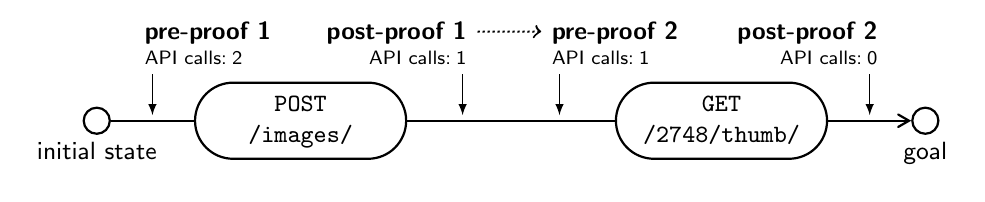
\begin{tikzpicture}[
      line width=.8pt,
      label distance = -1pt,
      state/.style = {
        circle, fill=white, draw=black,
        prefix after command={\pgfextra{\tikzset{
          every label/.style={black}, font=\small,
        }}},
      },
      request/.style = {
        rounded rectangle, draw=black, fill=white,
        text width=60pt, text depth=12pt, inner sep=5pt, align=center,
        font=\ttfamily\fontsize{9pt}{11pt}\selectfont\bfseries,
      },
      connector/.style = {
        black, line width=.8pt, -angle 60,
      },
      proof/.style = {
        black, draw,
        shorten <=2pt, shorten >=11pt, latex-,
        font=\small, inner sep=-2pt,
      },
      pretopost/.style = {
        black, draw, line width=.8pt, densely dotted, ->,
      },
      preproof/.style  = { align=left,  anchor=west, xshift=-.9pt },
      postproof/.style = { align=right, anchor=east, xshift=-.4pt },
      node distance = 75pt,
    ]
    \node[state,label=below:initial state] (Initial) {};
    \node[request,right=30pt of Initial] (POST) {POST\\ /images/};
    \node[request,right=of POST] (GET) {GET\\ /2748/thumb/};
    \node[state,label=below:goal,right=30pt of GET] (Goal) {};
    \begin{pgfonlayer}{background}
      \draw[connector] (Initial) -- (Goal);
    \end{pgfonlayer}
    \path[proof] (POST.west) ++(-15pt,0pt) -- ++(0pt,28pt)
      node[preproof]  {\textbf{\itshape pre-proof~1}\\[-2pt]\scriptsize API calls:~\kern-.2ex 2};
    \path[proof] (POST.east) ++(+20pt,0pt) -- ++(0pt,28pt)
      node[postproof] {\textbf{\itshape post-proof~1}\\[-2pt]\scriptsize API calls:~\kern-.2ex 1};
    \path[proof] (GET.west)  ++(-20pt,0pt) -- ++(0pt,28pt)
      node[preproof]  {\textbf{\itshape pre-proof~2}\\[-2pt]\scriptsize API calls:~\kern-.2ex 1};
    \path[proof] (GET.east)  ++(15pt,0pt)  -- ++(0pt,28pt)
      node[postproof, xshift=1.4pt] {\textbf{\itshape post-proof~2}\\[-2pt]\scriptsize API calls:~\kern-.2ex 0};
    \makeatletter
    \pgfsys@transformcm{1}{0}{0.23}{1}{-8pt}{0pt}
      \path[pretopost] ($(POST.east) + (26.0pt,32.2pt)$) -- ($(GET.west) + (-26pt,32.2pt)$);
    \makeatother
  \end{tikzpicture}
  \caption{A~proper post-proof of one operation becomes the pre-proof of the next.}
  \label{fig:Proofs}
\end{figure}

\subsection{Anatomy of a~Hypermedia API Composition Proof}
\label{sec:ProofAnatomy} 

Applied on a API composition problem, we get the following consequence:
\begin{corollary}[Correctness of API composition proofs]
Let $(H,g,R,B)$ be an API composition problem and $g'$ an instance  of $g$ then the following holds:
\[\text{If }H\cup R \cup B \vdash g' \text{ then }H\cup R \cup B \models g'\]
\end{corollary}

%The corollary ensures that every proof we get for an API composition problem is actually an evidence for the
%The corrollary ensures that every proof we get by applying the calculus is actually correct. 
%Unfortunately, the proof calculus is not complete
%as the following example shows: 


% According to the semantics introduced in chapter \ref{nthree} from \[\texttt{\{\{<a><b><c>.\}=> false.\}=> false.\}.}\] 
%  follows \[\texttt{<a><b><c>.}\]%although this holds with the definition of the semantics introduced in chapter \ref{nthree}. \\
%  As there is proof-step similar to $\bot$-elimination in first order logic, this cannot be shown applying the introduced calculus.
%  
 


We will examine the generalized modus ponens in more detail,
as this is the proof step where implication rules, 
such as \restdesc descriptions, are applied.

\label{sec:Reasoning}
\begin{lemma}\label{lemma:Reasoning}
Let $A$ be an \nthree alphabet, %$\Gamma\subset F$ a set of formulas, 
$f\in F_g$ a simple ground formula and $\verb!{!f_1\verb!}=>{!f_2\verb!}!\in F$ a simple implication formula %of nesting level 2 
where all 
universal variables which occur in $f_2$ %do 
also occur in $f_1$. If the generalized modus ponens is applicable to $f$ and $\verb!{!f_1\verb!}=>{!f_2\verb!}!$ then
the resulting formula does not contain universal variables.
\end{lemma}

\begin{proof}
 %Let  $\mu_{1}, \ldots, \mu_{n}$ be 
 %universal replacements 
 Let $\sigma:V_U\rightarrow E_e$ be a substitution %such that 
 such that  $(\verb!{!f_1\verb!}=>{!f_2\verb!}.!)\sigma^t= \verb!{!f\verb!}=>{!f_2'\verb!}.!$ 
As $f$ is a ground formula, $\text{range}(\sigma|_{V_U\cap(\text{comp}^1(f_1)\cup \text{comp}^2(f_1))}) \subset E_g$. 
Due to the condition that every universal variable of $f_2$ 
is also in $f_1$, i.e. 
\[((\text{comp}^1(f_2)\cup \text{comp}^2(f_2))\cap V_U )\subset (\text{comp}^1(f_1)\cup \text{comp}^2(f_1))\cap V_U)\]
the claim follows. 
%
 %As the implication
 %has nesting level 2, by Definition \ref{repl}, from each replacement only the first substitution $\sigma^{\mu_i}_{11}=: \sigma_{\mu_i}$ 
 %gets totally applied to the whole implication 
 %and we obtain
 %there are, by definition \ref{repl}, some substitutions $\sigma_1\ldots\sigma_n$ such that 
 %\[\mu_{1}\circ\ldots\circ\mu_{n}(\verb!{!f_1\verb!}=>{!f_2\verb!}.!)=(\verb!{!f_1\verb!}=>{!f_2\verb!}.!)\sigma_{\mu_1}^t\ldots\sigma_{\mu_n}^t.\]
 %Therefore all 
 %universal variables which are replaced in $f_1$ are also replaced by the same substitution in $f_2$.
\end{proof}


As \http requests in \restdesc descriptions only contain
one leading existential to represent the \http message, and 
\restdesc descriptions 
fulfill the conditions of Lemma~\ref{lemma:Reasoning}
%have nesting level~2,
we arrive at the following consequence:

\begin{corollary}
\label{corollary}
Every application of a ~restdesc description to a ground formula results in a~sufficiently specified \http request 
and a postcondition which does not contain any universal variables.
\end{corollary}

% Additional to the above mentioned steps proof steps themseves, %, the reasoner is able to apply existential renaming. 
% the substitutions done during the reasoning process %as well as those applied in generalized modus ponens 
% can be 
% described by the vocabulary\footnote{The vocabulary's rdf definition can be found at: \url{http://www.w3.org/2000/10/swap/reason\#}.}.
%Additional to the replacements done during the application of the generalized modus ponens, the proofs shown within this paper will also include existential renaming. 
%Although this is not expressed as a proof step cannot be expressed as a proof step, the vocabulary provides the opportunity to describe the substitutions made in such a pre-step.
%The reasoning vocabulary\footnote{The vocabulary's definition can be found at: \url{http://www.w3.org/2000/10/swap/reason\#}.}
%enables us to name the aforementioned proof steps. 
%their outcome, and the resources used to come to a conclusion. 
% The first step of Definition \ref{proofsteps} includes from a technical point of view also the parsing of a source.
% In the \nthree proof vocabulary%
% \footnote{The vocabulary's RDF definition can be found at: \url{http://www.w3.org/2000/10/swap/reason\#}.}
% we will discuss next,
% this step is therefore named after this action.
% 
% \begin{definition}[Proof vocabulary]
% Let $A$ be an \nthree alphabet and $\mathfrak{I}=(\mathcal{D}, \mathfrak{a}, \mathfrak{p})$ be an 
% interpretation of its formulas. Let $\verb!x!, \verb!y!,  \verb!y!_1, \ldots, \verb!y!_n \in U$ be \nthree representations of 
% proof steps and $\verb!z!_1,\verb!z!_2,\verb!z!_3\in U$.
% \begin{enumerate}
%  \item 
%  Proof step types:
%  \begin{itemize}
% \item $\mathfrak{I}\models \verb!x a r:Proof.!$ iff \verb!x! is the proof step which leads to the proven result.
% \item $\mathfrak{I}\models \verb!x a r:Parsing.!$ iff \verb!x! is a parsed axiom. %This step involves parsing the resources.
% \item $\mathfrak{I}\models \verb!x a r:Conjunction.!$ iff \verb!x! is a conjunction introduction.
% \item $\mathfrak{I}\models \verb!x a r:Inference.!$ iff \verb!x! is a generalized modus ponens.
% \item $\mathfrak{I}\models \verb!x a r:Extraction.!$ iff \verb!x! is a conjunction elimination.
% \end{itemize}
%  \item 
%  Proof predicates:
% \begin{itemize}
% \item $\mathfrak{I}\models \verb!x r:gives {!f\verb!}!$. iff $f\in F$ is the formula obtained by applying \verb!x!.
% \item $\mathfrak{I}\models \verb!x r:source u!$. iff \verb!x! is a parsed axiom and $\verb!u!\in U$ is the \uri of the %parsing's 
% parsed axiom's
% source. 
% \item $\mathfrak{I}\models \verb!x r:component y!$. iff \verb!x! is a conjunction introduction and $\verb!y!$ is a proof step which gives one of its components.
% \item $\mathfrak{I}\models \verb!x r:rule y.!$ iff \verb!x! is a generalized modus ponens and $\verb!y!$ is the proof step which leads to the applied implication.
% \item $\mathfrak{I}\models \verb!x r:evidence (y!_1,\ldots,\verb!y!_n\verb!)!$. iff \verb!x! is a generalized modus ponens and $\verb!y!_1,\ldots, \verb!y!_n$ 
% are the proof steps which lead to the formulas used for the unification with the antecedent of the implication.
% \item $\mathfrak{I}\models \verb!x r:because y!$. iff \verb!x! is a conjunction elimination and $\verb!y!$ is the proof step which yields the to-be-eliminated conjunction.
% \end{itemize}
% \item
% Substitutions:
% \begin{itemize}
%  \item $\mathfrak{I}\models \verb!x r:binding z!_1.$ iff \verb!x! includes a substitution $\verb!z!_1$.
%  \item $\mathfrak{I}\models \verb!z!_1 \verb! r:variable z!_2.$ iff $\verb!z!_1$ is a substitution whose domain is $\{\verb!z!_2\}$.
%  \item $\mathfrak{I}\models \verb!z!_1 \verb! r:boundTo z!_3.$ iff $\verb!z!_1$ is a substitution whose range is $\{\verb!z!_3\}$.
% \end{itemize}
% 
% \end{enumerate}
% \end{definition}
% 
% To produce a proof for an API composition problem, the reasoner needs to be aware of all formulas at its disposal (in our case $H \cup R \cup B$) and of the goal 
% which it is expected to prove.
% The latter is given to the reasoner as the consequence of a~\textit{filter rule}
% $\verb!{!f\verb!} => {!g\verb!}.!$%, the \textit{filter rule}.
% This triggers the reasoner to prove an instance of~$f$ and in case of success,
% return each provable ground instance of $g$ if possible,
% or a provable instance containing existentials otherwise.
% For brevity, not all reasoners display every proof step in a proof:
% especially conjunction elimination and introduction are often omitted.
% However, to the best of our knowledge,
% all reasoners' proofs contain all applications of $\verb!r:Inference!$ leading to a goal~$g$,
% which allows us to measure a~proof's length by counting applications of the generalized modus ponens.

 \begin{lstlisting}[
  float=t,
  caption={The initial knowledge of the agent \emph{(agent\_knowledge.n3)}},
  label=lst:Knowledge]
§\textcolor{gray}{@prefix dbpedia: <http://dbpedia.org/resource/>.}§

<lena.jpg> a dbpedia:Image.
\end{lstlisting}

\begin{lstlisting}[
  float=t,
  caption={A filter rule expressing the agent's goal \emph{(agent\_goal.n3)}},
  label=lst:Goal]
§\textcolor{gray}{@prefix dbpedia-owl: <http://dbpedia.org/ontology/>.}§

{ <lena.jpg> dbpedia-owl:thumbnail ?thumbnail. }
=>
{ <lena.jpg> dbpedia-owl:thumbnail ?thumbnail. }.
\end{lstlisting}

\begin{lstlisting}[
  float=p,
  caption={Example hypermedia API composition proof},
  label=lst:Proof]
§\textcolor{gray}{@prefix dbpedia: <http://dbpedia.org/resource/>.}§
§\textcolor{gray}{@prefix dbpedia-owl: <http://dbpedia.org/ontology/>.}§
§\textcolor{gray}{@prefix ex: <http://example.org/image\#>.}§
§\textcolor{gray}{@prefix http: <http://www.w3.org/2011/http\#>.}§
§\textcolor{gray}{@prefix n3: <http://www.w3.org/2004/06/rei\#>.}§
§\textcolor{gray}{@prefix r: <http://www.w3.org/2000/10/swap/reason\#>.}§

§\bfseries<\#proof> a r:Proof, r:Conjunction;\label{ln:Proof}§
  r:component <#lemma1>;
  r:gives { <lena.jpg> dbpedia-owl:thumbnail _:sk3. }.

§\bfseries<\#lemma1> a r:Inference;\label{ln:Lemma1}§
  r:gives { <lena.jpg> dbpedia-owl:thumbnail _:sk3. };
  r:evidence (<#lemma2>);
  r:binding [ r:variable [ n3:uri "var#x0"]; r:boundTo [ n3:nodeId "_:sk3"]];
  r:rule <#lemma7>.
  
§\bfseries<\#lemma2> a r:Inference;\label{ln:Lemma2}§
  r:gives { _:sk4 http:methodName "GET".
            _:sk4 http:requestURI _:sk3.
            _:sk4 http:resp _:sk5.
            _:sk5 http:body _:sk3.
            <lena.jpg> dbpedia-owl:thumbnail _:sk3.
            _:sk3 a dbpedia:Image.
            _:sk3 dbpedia-owl:height 80.0. };
  r:evidence (<#lemma3>);
  r:binding [ r:variable [ n3:uri "var#x0"]; r:boundTo [ n3:uri "lena.jpg"]];
  r:binding [ r:variable [ n3:uri "var#x1"]; r:boundTo [ n3:nodeId "_:sk3"]];
  r:binding [ r:variable [ n3:uri "var#x2"]; r:boundTo [ n3:nodeId "_:sk4"]];
  r:binding [ r:variable [ n3:uri "var#x3"]; r:boundTo [ n3:nodeId "_:sk5"]];
  r:rule <#lemma4>.
  
§\bfseries<\#lemma3> a r:Inference;\label{ln:Lemma3}§
  r:gives { _:sk0 http:methodName "POST".
            _:sk0 http:requestURI "/images/".
            _:sk0 http:body <lena.jpg>.
            _:sk0 http:resp _:sk1.
            _:sk1 http:body <lena.jpg>.
            <lena.jpg> ex:comments _:sk2.
            <lena.jpg> ex:smallThumbnail _:sk3. };
  r:binding [ r:variable [ n3:uri "var#x0"]; r:boundTo [ n3:uri "lena.jpg"]];
  r:binding [ r:variable [ n3:uri "var#x1"]; r:boundTo [ n3:nodeId "_:sk0"]];
  r:binding [ r:variable [ n3:uri "var#x2"]; r:boundTo [ n3:nodeId "_:sk1"]];
  r:binding [ r:variable [ n3:uri "var#x3"]; r:boundTo [ n3:nodeId "_:sk2"]];
  r:binding [ r:variable [ n3:uri "var#x4"]; r:boundTo [ n3:nodeId "_:sk3"]];   
  r:evidence (<#lemma6>);
  r:rule <#lemma5>.
  
§\bfseries<\#lemma4> a r:Extraction;§§\label{ln:Lemma4}§ r:because [ a r:Parsing; r:source <desc_thumbnail> ].
§\bfseries<\#lemma5> a r:Extraction;§§\label{ln:Lemma5}§ r:because [ a r:Parsing; r:source <desc_images> ].
§\bfseries<\#lemma6> a r:Extraction;§§\label{ln:Lemma6}§ r:because [ a r:Parsing; r:source <agent_knowledge> ].
§\bfseries<\#lemma7> a r:Extraction;§§\label{ln:Lemma7}§ r:because [ a r:Parsing; r:source <agent_goal> ].
\end{lstlisting}

\newcommand\lineref[1]{[\textit{line~\ref{#1}}]}
\newcommand\linesref[2]{[\textit{lines~\ref{#1}--\ref{#2}}]}

%\newpage

\subsection{Discussion of a~Composition Proof Example}\label{example}
\subsubsection{\bfseries Overview}
\Cref{lst:Proof} displays an example of a hypermedia API composition proof.
In addition to the two \restdesc descriptions from \cref{lst:Thumbnail,lst:Images}
($R$ in an API composition problem),
it involves the goal file \cref{lst:Goal} (\texttt{\{g\} => \{g\}.})
and the input file \cref{lst:Knowledge} (the initial knowledge $H$).
%the purpose of which will be explained in \cref{sec:Composition}.
The proof, generated by EYE~\cite{eyepaper},
explains how, given an image, a~thumbnail of this image can be obtained.
Its main element is \verb!r:Proof!~\lineref{ln:Proof},
which is a~conjunction of different components, indicated by \verb!r:component!.
In this example, there is only one,
but there can be multiple.
The conclusion of the proof
(object of the \verb!r:gives! relation)
is the triple
\verb!<lena.jpg> dbpedia-owl:thumbnail _:sk3 !%
(with \verb!_:sk3! an existential variable).
This captures the fact that \verb!lena.jpg! has a~certain thumbnail,
which is the consequent of the filter rule in \cref{lst:Goal}.

\vspace{-1em}

\paragraph{\bfseries Extractions and inferences}
EYE represents \verb!r:extraction!s and \verb!r:inference!s as lemmata,
which can be reused in different proof steps.
The extractions, Lemmata~4 to~7~\linesref{ln:Lemma4}{ln:Lemma7}, are fairly trivial as none of the underlying formulas is a real conjunction and will therefore not be discussed in detail.
In this proof, they just give the formulas specified in \cref{lst:Thumbnail} to 4 with renamed variables.
The inferences describe the actual reasoning carried out
and thus merit a~closer inspection.
We will follow the path backwards from the proof's conclusion,
tracing back inferences until we arrive at the atomic facts
that are the starting point of the proof.

\vspace{-1em}

\paragraph{\bfseries Filter rule}
The justification for the conclusion
consists in this case of a~single component, namely Lemma~1~\lineref{ln:Lemma1}.
This lemma is an application of the modus ponens using the implication of Lemma~7,
which is the file \verb!agent_goal.n3! shown in \cref{lst:Goal}.
This rule has been instantiated 
according to the variable bindings indicated by \verb!r:binding!:
here, the variable \verb!?thumbnail! (\verb!var#x0!)
is bound to the existential variable \verb!_:sk3!.
The unification uses a part of the result of Lemma~2 as indicated by \verb!r:evidence!, the performed conjunction elimination is not listed in this proof.
\sloppy Substituting \verb!_:sk3! for \verb!?thumbnail! in \cref{lst:Goal}
indeed gives the desired conclusion
\verb!<lena.jpg> dbpedia-owl:thumbnail _:sk3!,
which contributes to the final~result.

\vspace{-1em}

\paragraph{\bfseries Thumbnail operation}
Lemma~2~\lineref{ln:Lemma2} is another \verb!r:inference!,
this time applying the rule from Lemma~4,
which is the \restdesc description in \cref{lst:Thumbnail}
that explains what happens when an image is uploaded. 
The instantiation is again detailed with \verb!r:binding! statements.
The \verb!?image! variable (\verb!var#x0!) is bound to \verb!lena.jpg!,
the \verb!?thumbnail! variable (\verb!var#1!) to the existential \verb!_:sk3!.
This is only possible because a~ statement
\verb!<lena.jpg> ex:smallThumbnail _:sk3! is proven; 
its derivation will be detailed shortly.
The other variables \verb!var#x2! and \verb!var#x3!
refer to the request and response resources in the consequent of \cref{lst:Thumbnail}
and are instantiated with new existentials (\verb!_:sk4! and \verb!_:sk5!).
This lemma is in turn made possible by another one.

\vspace{-1em}

\paragraph{\bfseries Upload operation}
Lemma~3~\lineref{ln:Lemma3} explains the derivation of the triple
that is a~necessary condition for Lemma~2:
\verb!<lena.jpg> ex:smallThumbnail _:sk3!.
The rule used for the inference is that
from the upload action in \cref{lst:Images} (Lemma~5),
instantiated with the initial knowledge of the agent
that it has access to an image (\cref{lst:Knowledge} / Lemma~6).
Substituting this knowledge into the rule
by binding \verb!?image! (\verb!var#x0!)
 to \verb!lena.jpg!,
gives the triples of the instantiated consequent,
as shown by the \verb!r:gives! predicate.
Note in particular the newly created existential \verb!_:sk3!;
this entails the triple \verb!<lena.jpg> ex:smallThumbnail _:sk3!
which is needed for Lemma~2.
Lemma~3 itself is justified by Lemma~6 (\cref{lst:Knowledge}),
which is a~simple extraction that stands on itself.
Hence, we have reached the starting proof's starting~point.

\vspace{-1em}

\paragraph{\bfseries From start to end}
As a~summary, we will briefly follow the proof in a~forward way.
Extracted from the background knowledge in \cref{lst:Knowledge},
the triple \verb!<lena.jpg> a dbpedia:Image!
triggers the image upload rule from \cref{lst:Thumbnail},
which yields \verb!<lena.jpg> dbpedia-owl:thumbnail _:sk3!
for some existential variable \verb!_:sk3!.
This triple in turn triggers the thumbnail rule from \cref{lst:Thumbnail},
which yields \verb!<lena.jpg> ex:smallThumbnail _:sk3!.
Finally, this is the input for the filter rule from \cref{lst:Goal},
which yields the final result of the proof:
the image has some thumbnail.
So given the background knowledge
and the two hypermedia API descriptions,
this proof verifies that the goal follows from them.

\subsection{Hypermedia API Operations inside a~Proof}
The proof in \cref{lst:Proof} is special
in the sense that some of its implication rules,
namely \cref{lst:Thumbnail,lst:Images},
are actually hypermedia API descriptions.
That means they do not fulfill an actual ontological implication.
Instead, they convey dynamic information.
Therefore, those steps in the proof
can be interpreted as \http requests that should be performed
in order to achieve the desired result.
This proof is indeed a~pre-proof:
it is valid under the assumption
that the described \http requests will behave as expected,
which can never be guaranteed on an environment such as the Internet.
The instantiation of a~hypermedia API description
turns it into the description of a~concrete API operation.
For instance, Lemma~3~\lineref{ln:Lemma3} contains the following operation:
\begin{Verbatim}
    _:sk0 http:methodName "POST".
    _:sk0 http:requestURI "/images/".
    _:sk0 http:body <lena.jpg>.
    _:sk0 http:resp _:sk1.
    _:sk1 http:body <lena.jpg>.
    <lena.jpg> ex:comments _:sk2.
    <lena.jpg> ex:smallThumbnail _:sk3.
\end{Verbatim}
This instructs an agent to perform
an \http \verb!POST! request (\verb!_:sk0!) to \verb!/images/!
with \verb!lena.jpg! as the request body.
This request will return a~response (\verb!_:sk1!)
with a~representation of \verb!lena.jpg!,
which will contain \verb!ex:comments! and \verb!ex:smallThumbnail! links.
Since this is a~hypermedia API,
the link targets are not yet known at this stage.
Therefore, they are represented by generated existential variables \verb!_:sk2! and \verb!_:sk3!.
At runtime, the \http request will return the actual link targets,
but at the pre-proof stage,
it suffices to know that some target for those links will exist.

Indeed, the outcome of this rule---the fact that \emph{some} \verb!smallThumbnail! links will exist---%
serves as input for the next API operation in Lemma~2 \lineref{ln:Lemma2}.
The consequent of this rule is instantiated as follows:
\begin{Verbatim}
    _:sk4 http:methodName "GET".
    _:sk4 http:requestURI _:sk3.
    _:sk4 http:resp _:sk5.
    _:sk5 http:body _:sk3.
    <lena.jpg> dbpedia-owl:thumbnail _:sk3.
    _:sk3 a dbpedia:Image.
    _:sk3 dbpedia-owl:height 80.0
\end{Verbatim}
This describes a~\verb!GET! request (\verb!_:sk4!) to the URL \verb!_:sk3!,
which will return a~representation of a~thumbnail that is 80~pixels high.
This request is interesting because it is \emph{incomplete}:
\verb!_:sk3! is not a~concrete URL that can be filled in. 
However, this identifier is the same variable as the one in Lemma~3,
so this description essentially states
that whatever will be the target of the \verb!smallThumbnail! link in the previous \verb!POST! request
should be the URL of the present \verb!GET! request.
The existential variables thus serve as placeholders
for values that will be the result of actual API operations.

While the proof above is a~pre-proof,
a~proper post-proof can be obtained by actually executing the \verb!POST! \http request,
which has all values necessary for execution
(as opposed to the \verb!GET! request where the URL is still undetermined).
This execution will result in a~concrete value
for the \verb!comments! and \verb!smallThumbnail! link placeholders \verb!_:sk2! and \verb!_:sk3!.
They lead to a~proper post-proof that uses these concrete values,
and hence that proof does not need the assumption that the \verb!POST! request will execute successfully
(because evidence shows it did).
\Cref{fig:UmlDiagram} shows the UML sequence diagram
of an example interaction between the client and the server.


\begin{figure}
  \begin{sequencediagram}
  \renewcommand\unitfactor{0.4}
    \newthread[white]{c}{Client}
    \newinst[8]{s}{Server}
\scriptsize
    \begin{callself}{c}{Create pre-proof for the first operation (\cref{lst:Proof})}{}\end{callself}

    \begin{sdblock}{First operation}{}
      \begin{call}{c}{\texttt{POST /images/}}{s}
        {\textit{hypermedia representation~$R_1\thinspace$of \texttt{lena.jpg}}}
      \end{call}
    \end{sdblock}

    \begin{callself}{c}{Create post-proof after the first operation}
                       {this post-proof becomes the pre-proof for the second operation}\end{callself}

    \begin{sdblock}{Second operation}{}
      \begin{call}{c}{\texttt{GET /images/2748/thumb/} \textit{(via link found in~$R_1$)}}{s}
        {\textit{hypermedia representation~$R_2\thinspace$of a~thumbnail of \texttt{lena.jpg}}}
      \end{call}
    \end{sdblock}
  \end{sequencediagram}
  \caption{
    The \emph{a~posteriori} UML sequence diagram of an example execution
    shows how the second operation happened through a~link in the first operation.
  }
  \label{fig:UmlDiagram}
\end{figure}
\normalsize

As stated in its definition,
a~pre-proof implicitly assumes that each API will indeed deliver the functionality
as stated in its \restdesc description.
The proof thus only holds under that assumption.
For example, if a~power outage occurs during the calculation of the aspect ratio,
the placeholder will not be instantiated with an actual value during the execution,
which can pose a~threat to subsequent hypermedia API operations that depend on this value.
However, the failure of a~single API operation
does not necessarily imply the intended result cannot be achieved.
Rather, it means the assumption of the pre-proof was invalid
and an alternative pre-proof---a~new hypermedia API composition---should be created,
starting from the current application state.
Such a~pragmatic approach to proofs containing hypermedia API operations is unavoidable:
no matter how low the probability of a~certain operation to fail,
failures can never be eliminated.
Therefore, pragmatism ensures that planning in advance is possible.
Each proof should be stored along with its assumptions
in order to understand the context it which it can be used.

\section{Hypermedia-driven Composition Generation and Execution}
\label{sec:Composition}
In contrast to fully plan-based methods,
the steps in the composition obtained through reasoner-based composition of hypermedia APIs
are not executed blindly.
Instead, the interaction is driven by the hypermedia responses from the server;
the composition in the proof only serves as \emph{guidance} for the client,
and as a~guarantee (to the extent possible) that the desired goal can be reached.
The composition that starts from the current state
helps an agent decide what its next step towards that goal should be.
Once this step has been taken, the rest of the pre-proof is discarded
because it is based on outdated information.
After the request,
the state is augmented with the information inside the server's response.
This new state becomes the input for a~new pre-proof
that takes into account the actual situation,
instead of the expected (and incomplete) values from the hypermedia API description.
In this section, we will detail this iterative composition generation
and execution.

\subsection{Goal-oriented Composition Generation}
Creating a~composition that satisfies a~goal comes down
to generating a~proof that supports the goal.
Inside this proof, the necessary hypermedia API operations will be incorporated as instantiated rules.
Proof-based composition generation,
unlike other composition techniques,
requires no composition-specific tools or algorithms.
A~generic reasoner that supports the rule language in which the hypermedia APIs are described
is capable of generating a~proof containing the composition.
For example, since \restdesc descriptions are expressed in the \nthree language,
compositions of hypermedia APIs described with \restdesc
can be performed by any \nthree reasoner with proof support.
The fact that proof-based composition can be performed by existing reasoners
is an advantage in itself,
because no new software has to be implemented and tested.
Furthermore, this offers the following benefits.
\begin{description}
\item[Incorporation of external knowledge]
  Existing RDF knowledge can directly be incorporated into the composition process.
  Whereas composition algorithms that are specifically tailored to certain description models
  usually operate on closed worlds,
  generic Semantic Web reasoners are built to incorporate knowledge from various sources.
  For example, existing OWL and RDF ontologies can be used
  to compose hypermedia APIs described with different vocabularies.
\item[Evolution of reasoners]
  Many implementations of reasoners exist
  and they continue to be updated to allow enhanced performance and possibilities.
  The proof-based composition method directly benefits from these innovations.
  This also counters the problem that many single-purpose composition algorithms
  are seldom updated after their creation because they are so specific.
\item[Independent validation]
  When dealing with proof and trust on the Web,
  it is especially important that the validation can happen by an independent party.
  Since different reasoners and validators exist,
  the composition proof can be validated independently.
  This contrasts with other composition approaches,
  whose algorithms have to be trusted.
\end{description}

In order to make a~reasoner generate a~pre-proof of a~composition,
it must be invoked with the initial state, the available hypermedia APIs, and the desired goal.
Here, we will examine the case for \nthree reasoners
and hypermedia APIs described with \restdesc\ \nthree rules,
but the principle of proof-based composition is generalizable
to all families of inference rules.

The hypermedia API descriptions include all those APIs available to the client.
In practice, the number of supplied available hypermedia APIs
would be substantially higher than the number of APIs in the resulting composition.
The background knowledge can, for example, consist of ontologies and business rules.
The reasoner will try to infer the goal state,
asserting the other inputs as part of the ground truth.
The initial state and background knowledge should correspond to reality,
regardless of the results of the actual execution,
provided the descriptions are accurate.
In contrast, the API description rules only hold under the assumption of successful execution,
due to the nature of the pre-proof.

%\clearpage

If the reasoner can infer the goal state given the ground truth,
we can conclude that a~composition \emph{exists}.
To obtain the details of the composition,
the reasoner must return the proof of the inference,
i.e., the data and rules applied to achieve the goal.
Inside this proof,
there will be placeholders for return values by the server
that are unknown at design-time.
The proof will be structured as in \cref{lst:Proof},
where the initial state was \cref{lst:Knowledge},
the goal state \cref{lst:Goal},
and the descriptions \cref{lst:Thumbnail,lst:Images}.
No background knowledge was needed,
but it could have been useful for instance
if the image of the initial state was described in different ontology,
in which case the conversion to the \dbpedia ontology would be necessary.

\subsection{Hypermedia-driven Execution}
\label{subsec:Execution}
In order to achieve a~certain goal in a~hypermedia-driven way,
the following process steps can be followed.
\begin{definition}[Pragmatic proof algorithm]
\label{def:PPAlgorithm}
Given an API composition problem with an initial state $H$, goal $g$,
description formulas $R$ and background knowledge $B$,
we define the pragmatic proof algorithm as follows:
\begin{enumerate}
\item
  Start an \nthree reasoner to generate a pre-proof for $(R, g, H, B)$. %$g$ by using  $\verb!{!g\verb!}=>{!g\verb!}!.$ as a 
  %filter rule and applying the knowledge and rules from $H, B$ and $R$. 
  \begin{enumerate}
  \item If the reasoner is not able to generate a proof, halt with \emph{failure}.
  %\item If the there exists a proof and this proof does not contain any rule of $R$, halt with \emph{success}.
  \item Else scan the pre-proof for applications of rules of $R$, set the number of these applications to $n_{\text{pre}}$.
  \end{enumerate} 
  \item Check $n_{\text{pre}}$:
  \begin{enumerate}
  \item If $n_{\text{pre}}=0$%If the there exists a proof and this proof does not contain any rule of $R$, 
  %If no such application can be found
  , halt with \emph{success}.
  \item Else %store the number of applications of rules of $R$ as $n_{\text{pre}}$ and 
  continue with Step~3.
  \end{enumerate}
%   
% \item[1a.]
%   The existence of a~proof indicates that the goal can be reached
%   from the current state (under the assumption that all API operations behave as described).
%   If no proof can be~generated, the goal cannot be reached and the process terminates with \verb!fail!.
% \item[1b.]
%   If the proof does not make use of any element of $R$,
%   then the current state directly entails the goal
%   and the agent proceeds to Step~5.
\item
  Out of the pre-proof, select a sufficiently specified \http request description which is part of 
  the application of a rule $r\in R$.%\footnote{Because of corollary \ref{corollary} and definition \ref{apicomp}, this description always exists.}
\item  Execute the described HTTP request
  and parse the (possibly empty) server response to a set of ground formulas $G$. 
\item  Invoke the reasoner with the new 
  API composition problem $(R, g, H\cup G, B)$ to produce a post-proof.
%   \begin{enumerate}
%    \item If the reasoneris not able to produce a proof, go back to Step~1 with the new API composition problem $(R\setminus \{ r\}, g, H, B)$.
%    \item Else continue with Step 7.
%   \end{enumerate}
 \item  Determine $n_{\text{post}}$:
 \begin{enumerate}

 \item If the reasoner was not able to generate a~proof,
 set $n_{\text{post}}:=n_{\text{pre}}.$

%  \item If the reasoner was not able to generate a post-proof (e.g., failed integrity constraints),
%        set $n_{\text{post}}:=n_{\text{pre}}$

 \item Else scan the proof for the number of inference steps which are using rules from $R$ and set this number of steps to $n_{\text{post}}$.  
  %\footnote{Because of corollary \ref{corollary} and definition \ref{apicomp}, this description always exists.}
  \end{enumerate}
  \item Compare $n_{\text{post}}$ with $n_{\text{pre}}$:
 \begin{enumerate}
 %\item If the execution fails, go back to step 1 with the new reduced set of \restdesc rules $R_{new}:= R\setminus \{r\}$.
 \item If $n_{\text{post}} \geq n_{\text{pre}}$ %the number of Inferences using rules from $R$ is not lower than in the pre-proof, %HTTP requests %the execution succeeds, parse the server's response 
	go back to Step~1 with the new API composition problem $(R\setminus \{ r\}, g, H, B)$. %with the new reduced set of \restdesc rules $R_{new}:= R\setminus \{r\}$.
 \item If $n_{\text{post}} < n_{\text{pre}}$, the post-proof
 can be used as the next pre-proof.
       Set $n_{\text{pre}}:=n_{\text{post}}$ and continue with Step~2.
 \end{enumerate}
%   \item[3.]
%   The \http request is executed to perform the API operation.
%   After that the server's response is parsed
%   and the resulting set of ground formulas $G$ is added to the existing state to get a new state $H\cup G$.
% \item[4.]
%   The reasoner is invoked with the new state and the API descriptions
%   to generate a~post-proof.
% \item[4a.]
%   If the execution delivered a~result matching the expectations,
%   the proof now contains one less \verb!r:inference! step
%   as the proof can now directly use the obtained knowledge
%   instead of instantiating a~hypermedia API description with placeholders.
%   The \emph{post}-proof of this iteration
%   corresponds to the next iteration's \emph{pre-}proof,
%   starting from the next Web~API~operation.
%   Proceed with Step~1b.
% \item[4b.]
%   If the number of \verb!r:inference! applications is not lower, or the reasoner detects that there exists no model for $H\cup G$, $B$, $R$ and $g$,
%   the hypermedia API did not deliver the expected result.
%   In that case, we can no longer rely on the corresponding API description,
%   it is removed from $R$.
%   Proceed with Step~1 using $H, B, g$ and the reduced  set of description formulas.
% \item[5.]
%   If no API operations are left in the proof, its result is reported to the user
%   and the process terminates successfully.
  
\end{enumerate}
\end{definition}

Before having a more theoretical look at the results of this algorithm,
let us run through a~possible execution
of the composition example introduced previously.

\newcommand\stepref[1]{\emph{(Step~#1)}}
\begin{itemize}
  \item \stepref{1} Given the background knowledge, initial state, and goal,
        the reasoner generates the pre-proof from \cref{lst:Proof},
        which contains $n_{\text{pre}} = 2$ API operations.
  \item \stepref{2} $n_{\text{pre}} \neq 0$, so continue with Step~3.
  \item \stepref{3} The HTTP request to upload the image
        is the only one that is sufficiently instantiated,
        so it is selected.
  \item \stepref{4} Execute the \http request
        by posting the image to \verb!/images/!,
        and retrieve a~hypermedia response.
        Inside this hypermedia response,
        there is a~\verb!comments! link to \verb!/comments/about/images/37!
        and a~\verb!smallThumbnail! link to \verb!/images/37/thumb/!.
        They are added to~$G$.
  \item \stepref{5} A~post-proof is produced from the new state,
        revealing that the goal can now be completed with one API operation.
        Indeed, only an \http \verb!GET! request to \verb!/image/37/thumb! is needed.
  \item \stepref{6} The above means that $n_{\text{post}} = 1$.
  \item \stepref{7} $n_{\text{post}} = 1 < n_{\text{pre}} = 2$,
        so set $n_{\text{pre}} := 1$ and continue with Step~2.
  \item \stepref{2} $n_{\text{pre}} = 1 \neq 0$, so continue with Step~3.
  \item \stepref{3} Select the only remaining HTTP request in the pre-proof.
  \item \stepref{4} Execute the \verb!GET! request to \verb!/image/37/thumb!
        and thereby obtain a~representation of the thumbnail of the image.
  \item \stepref{5} Generate the post-proof;
        it consists entirely of data
        as the necessary information to reach the goal has been obtained.
  \item \stepref{6} No rules of~$R$ are applied, so $n_{\text{post}} = 0$.
  \item \stepref{7} $n_{\text{post}} = 0 < n_{\text{pre}} = 1$,
        so set $n_{\text{pre}} := 0$ and continue with Step~2.
  \item \stepref{2} $n_{\text{pre}} = 0$, so halt with \textit{success}.
\end{itemize}

\noindent
This example shows how the proof guides the process,
but hypermedia drives the interaction.
For instance, the \URL needed for the \verb!GET! request was not hard-coded:
it was obtained as a~hypermedia control from the server.
This means that, even if the server changes its internal \URL structure
or the layout of the representation,
the interaction can still take place.
The client needs the RESTdesc descriptions to find out whether the complex goal is possible
and what first steps it should take.
Otherwise, it would have no way of knowing
that the upload of an image results in a~link to the thumbnail.
However, once this expectation is there,
the client navigates through hypermedia.
We can compare this to driving with a~map:
the map gives the overall picture,
but the actual wayfinding happens based on the actual roads and scenery
when somebody undertakes the journey.

There are several reasons, why the situations in 1(a) or 6(a) can occur:
the reasoner could have a~technical problem, it could detect inconsistencies
(a fulfilled antecedent of a rule with false in the consequent), it could simply be that 
there is no instance $g'$ of $g$ which is a logical consequence of $H \cup R\cup B$, but even
if such a $g'$ exists the reasoning problem is undecidable.
This is because RESTdesc descriptions are rules with new existential variables in the consequence,
which makes the problem in general undecidable, as discussed by \cite{Baget}.

%\clearpage
%\noindent
However, we can show that the following holds:
\begin{theorem}
Given an execution of the algorithm in \cref{def:PPAlgorithm}
that requires $n$~executions of the reasoner (in Steps 1 and~5).
If all $n$~reasoning runs terminate, the algorithm terminates as well.
Furthermore, if the algorithm halts with \emph{success},
its output is a~ground instance of the goal state.

\end{theorem}

\begin{proof}
We first show termination:
if the algorithm does not terminate, it especially never reaches the Steps 1(a) and 2(a) and
%
Steps 1 and 2 always result in option (b). 
%We take a closer look to the proofs checked in Step 3:
All formulas in $H\cup B$ are either ground formulas
or simple rule formulas % of level~2 
which do not contain existentials 
and which fulfill Lemma~\ref{lemma:Reasoning}.
Therefore no atomic formula or conjunction of atomic formulas
which can be obtained by applying the proof steps from Definition \ref{proofsteps}
on $H\cup B$
contains universals %of nesting level 1 
or existentials.
If for a pre-proof $n_{\text{pre}}>0$ holds, it must 
%therefore, the results of the application of these rules are ground
%For a pre-proof that contains at least one application of a \restdesc rule it follows
%with 
by Corollary~\ref{corollary} %and definition \ref{apicomp} %follows that if a pre-proof contains 
%every pre-proof for an API composition problem 
%that it contains a 
contain at least one
sufficiently specified \http request description. So, Step 3 and the following Steps~4--6 can always be executed.
%this description always exists.
Step 7(a) reduces the set of \restdesc descriptions, it can only be performed $|R|$ times.
Starting from a fixed pre-proof $\text{pre}_0$, Step~7(b) can only be applied $n_{\text{pre}_0}$ times.
Thus, the algorithm terminates.%\\

As every operation which changes the API composition problem for the pre-proof to be checked in Step 2, preserves the syntactic properties of the 
sets of formulas involved, it is enough to show that the result of every pre-proof of an API composition problem which does not contain 
applications of \restdesc rules is ground. %This is the case because of the properties
This follows by the same arguments as above. As $H\cup B \cup \{ \texttt{\underline{\{}g\underline{\}} => \underline{\{}g\underline{\}}.}\}$ 
only contains ground formulas and rules which fulfill
the conditions of Lemma~\ref{lemma:Reasoning},
it is not possible to derive atomic formulas or conjunctions of atomic formulas which contain existentials or universals %at nesting level 1,
thus the result of the proof is ground.
% If the algorithm succeeds, it ends with Step~3, resulting in the proven \nthree formula $g'$ which,
% by definition of the filter, is an instance or a conjunction
% of instances of the goal $g$. If $n(g)=0$, $g=g'$ is the only instance of $g$.
% It remains to prove, that, if $n(g)=1$,  $g'$ is ground.
% 
% If Step 2.(a) detects that a proof generated in Step~1 or~6 
% does not contain any application of rules of~$R$,
% all formulas used in the proof are either ground formulas
% or rules of level~2 which do not contain existentials %in the consequences
% and which fulfill Lemma~\ref{lemma:Reasoning};
% therefore, the results of the application of these rules are ground---thus $g'$ is ground.
% 
% If the proof contains applications of rules of $R$, there is at least one application of such a rule 
% to a formula of the initial state or one of its ground consequences 
% derived using the background knowledge or conjunction elimination or introduction.
% The consequence of that rule contains by Corollary~\ref{corollary} a sufficiently specified \http request description.
% 
% This \http request description will be selected in Step~4 and executed in Step~5.
% Since a~successful application solely adds ground instances $G$ to $H$,
% the post-proof---if the reasoner finds one---%
% has the same formal properties as the pre-proof.
% 
% If the reasoner is not able to find a post-proof,
% Step~8(a) only reduces the set $R$ and starts again with Step~1, 
% therefore the new pre-proof will have the same formal properties 
% as the first pre-proof generated.
%the proper post-proof generated in Step~6
%will have the same properties as described above.
\end{proof}

% \subsection{Semi-Automated Description Generation}
% \label{sec:Generation}
% One of the bottlenecks with traditional description-based methods of Web APIs and services
% is that these descriptions have to be created, which is mostly a~manual task.
% Consequently, without a~method that facilitates the creation of such descriptions,
% the overall concept of description-based composition and execution
% might not successfully transition from theory to practice.
% This section explains how RESTdesc descriptions can be created
% by a~computer-assisted process.
% 
% We define \emph{semi-automated RESTdesc description generation}
% as a~process that takes as input a~series of HTTP requests and responses
% performed by one or more persons,
% and provides as output skeletons for RESTdesc descriptions,
% which a~user can then further refine to a~final description.
% We rely on the fact that RESTdesc descriptions
% capture the \emph{expectations} of resources.
% For example, \cref{lst:Images} captures the expectation that
% the upload of an image will result in links to comments and a~thumbnail.
% RESTdesc thus describes the generic hypermedia controls
% that will be available on such image resources.
% 
% \begin{lstlisting}[
%   float=t,
%   caption={
%     Example user interaction with a~Web API,
%     used as input for the RESTdesc description generation process.
%   },
%   label=lst:Interaction]
% §\textbf{HTTP request~1: POST to /images/ with image1.jpg as body}§
% §\textbf{HTTP response~1:}§
% @prefix ex: <http://example.org/image#>.
% @prefix dbpedia: <http://dbpedia.org/resource/>.
% 
% </images/24> a dbpedia:Image.
%              ex:comments </images/24/comments>.
%              ex:smallThumbnail </images/24/thumbnail>.
% 
% 
% §\textbf{HTTP request~2: GET to /images/24/thumbnail}§
% §\textbf{HTTP response~2:}§
% @prefix dbpedia: <http://dbpedia.org/resource/>.
% @prefix dbpedia-owl: <http://dbpedia.org/ontology/>.
% 
% </images/24> dbpedia-owl:thumbnail </images/24/thumbnail>.
% </images/24/thumbnail> a dbpedia:Image;
%                        dbpedia-owl:height 80.0.
% 
% 
% §\textbf{HTTP request~3: POST to /images/ with image2.jpg as body}§
% §\textbf{HTTP response~3:}§
% @prefix ex: <http://example.org/image#>.
% @prefix dbpedia: <http://dbpedia.org/resource/>.
% 
% </images/25> a dbpedia:Image.
%              ex:comments </images/25/comments>.
%              ex:smallThumbnail </images/25/thumbnail>.
% 
% 
% §\textbf{HTTP request~4: GET to /images/25/thumbnail}§
% §\textbf{HTTP response~4:}§
% @prefix dbpedia: <http://dbpedia.org/resource/>.
% @prefix dbpedia-owl: <http://dbpedia.org/ontology/>.
% 
% </images/25> dbpedia-owl:thumbnail </images/25/thumbnail>.
% </images/25/thumbnail> a dbpedia:Image;
%                        dbpedia-owl:height 80.0.
% \end{lstlisting}
% 
% The idea behind the process is
% to extract the hypermedia controls from a~series of requests performed by people.
% We will describe the strategy using an exemplary series of interactions,
% displayed in \cref{lst:Interaction}.
% To create this particular series,
% a~user uploaded two images and obtained their thumbnails.
% 
% First, the process needs to identify the different kinds of steps and thus resources.
% This happens by performing clustering on the HTTP responses with, for instance,
% a~string similarity algorithm as distance function.
% In this case, responses 1 and~3 are highly similar,
% and so are responses 2 and~4.
% Therefore, they are assigned into two different clusters.
% Note that such clustering is especially realistic
% because Web APIs typically generate responses based on templates,
% which contributes to a~high structural similarity
% for responses of the same kind that hence follow the same template.
% User interaction can influence the clustering sensitivity,
% and possibly manually change assignments.
% Since the two clusters, corresponding to 2 types of operations,
% are correct in this example, nothing needs to change.
% 
% Next, for each cluster,
% the common elements in responses and their corresponding requests are identified.
% In this case, the first cluster contains two \verb!POST! requests to \verb!/images/!,
% and both responses contain some resource that is an image,
% and has a~link to comments and images.
% This allows the algorithm to produce a~skeleton as follows:
% \begin{Verbatim}
% { ?object1 a :localFile. }
% =>
% {
%   _:request http:methodName "POST";
%             http:requestURI "/images/";
%             http:body ?object1;
%             http:resp [ http:body _:object2 ].
%   _:object2 a dbpedia:Image;
%             ex:comments _:object3;
%             ex:smallThumbnail _:object4.
% }
% \end{Verbatim}
% Note how this is very close to \cref{lst:Images}.
% The user can still improve this description
% by specifying that \verb!?object1! and \verb!_object2! are the same entity,
% and that \verb!?object1! is a~\verb!dbpedia:Image! already in the antecedent.
% After these changes, and possibly renaming variables and blank nodes for legibility,
% the description is the same as that of \cref{lst:Images} and thus correct.
% 
% Identifying common elements in the second cluster
% leads to the following skeleton:
% \begin{Verbatim}
% {}
% =>
% {
%   _:request http:methodName "GET";
%             http:requestURI _:object1;
%             http:resp [ http:body _:object1 ].
%   _:object2 dbpedia-owl:thumbnail _:object1.
%   _:object1 a dbpedia:Image;
%             dbpedia-owl:height 80.0.
% }.
% \end{Verbatim}
% The fact that the request~URI and the body refer to the same entity (\verb!_:object1!)
% can be deduced from the properties of the \verb!GET! method in the HTTP specification.
% These properties do not apply to \verb!POST!,
% which is why the previous skeleton could not make this assumption.
% The current skeleton is still incomplete, since it does not have a~precondition.
% More specifically, we need to obtain the request~URI somehow.
% Given the sequence of the requests in \cref{lst:Interaction},
% the process can detect that the concrete instances of \verb!_:object1!
% (\verb!/images/24/thumbnail! and \verb!/images/25/thumbnail!)
% were already mentioned in a~previous response body.
% Hence, it can place the pattern containing those instances in the antecedent
% and connect the components that had identical values with the same variable names:
% \begin{Verbatim}
% { ?object2 ex:smallThumbnail ?object1. }
% =>
% {
%   _:request http:methodName "GET";
%             http:requestURI ?object1;
%             http:resp [ http:body ?object1 ].
%   ?object2 dbpedia-owl:thumbnail ?object1.
%   ?object1 a dbpedia:Image;
%            dbpedia-owl:height 80.0.
% }.
% \end{Verbatim}
% The user can now optionally rename the variable placeholders
% to obtain the exact same description as in \cref{lst:Thumbnail}.
% 
% This shows how descriptions such as \cref{lst:Thumbnail,lst:Images}
% can be generated.
% Note that this process is not fully automated, but human-assisted.
% That is, it requires a~repeated sequence of human steps as input
% in order to sufficiently cluster and generalize descriptions.
% Furthermore, hints and corrections from users might be necessary,
% as over- or undergeneralizations will occur inevitably in some cases.
% Yet such an assisted process significantly decreases the burden
% of full manual description.
% The fact the RESTdesc descriptions focus on REST APIs facilitates the process:
% it can make additional assumptions on the behavior of the uniform interface,
% and hyperlinks from previous responses can be reused.
% 
% Most important for this assisted generation of descriptions
% is the close relationship between N3 and RDF.
% As we have shown above, the RDF triples in the Web API's responses
% serve as a~direct prototype for the consequent of the generated skeletons.
% For example, the triple
% \verb!</images/24>! \verb!dbpedia-owl:smallThumbnail! \verb!</images/24/thumbnail>.!
% directly leads to the inclusion of
% \verb!_:object2! \verb!dbpedia-owl:smallThumbnail! \verb!_:object4!
% in the first skeleton.
% Not only does this simplify the generation process,
% the connection between the generated description
% and the original response is also apparent for users,
% which makes it easier for them as well.
% 

\todo{Cite \cite{verborgh_phd_2014} for evaluation.}
% 
% \section{Evaluation}
% \label{sec:Evaluation}
% \subsection{Composition Algorithm Benchmark}
% This article discusses a~proof-based method to compose and execute hypermedia APIs.
% Specific to this method, in contrast to traditional Web service composition methods,
% is that the composition should be regenerated at each step.
% This makes the feasibility of the approach depend
% on whether the composition cost is within reasonable limits.
% Therefore, an evaluation should assess whether
% composition happens sufficiently fast
% for realistic composition lengths
% and in presence of a~realistic number of possible hypermedia APIs
% that can be used in compositions.
% 
% To verify this, we developed a~benchmark framework%
% \footnote{Available at \url{http://github.com/RubenVerborgh/RESTdesc-Composition-Benchmark}.}
% for hypermedia API composition,
% consisting of two main components:
% \begin{description}
% \item[a~hypermedia API description generator]\hspace{-1ex},
% which deterministically generates single- or multi-connected chains
% of example hypermedia API descriptions with a~chosen length,
% specifically tailored to enable compositions;
% \item [an automated benchmarker]\hspace{-1ex},
% testing how well a~reasoner performs
% on creating proofs for compositions of varying lengths and complexity.
% \end{description}
% 
% Below is one of the example descriptions,
% generated by the tool with parameters \verb!3!~(description chain length)
% and \verb!2!~(number of needed connections per description).
% \begin{Verbatim}
%     {
%       ?a1 ex:rel2 ?b1.                 # Generated input conditions
%       ?a2 ex:rel2 ?b2.
%     }
%     =>
%     {
%       _:request http:methodName "GET"; # Generated HTTP request
%                 http:requestURI ?a1;
%                 http:resp [ http:body ?b1 ].
%       ?a1 ex:rel3 ?b1.                 # Generated output conditions
%       ?a2 ex:rel3 ?b2.
%     }.
% \end{Verbatim}
% 
% The goal would be a~filter rule of the following form:
% \begin{Verbatim}
%     {
%       ?a1 ex:rel3 ?b1.                 # Output conditions of the
%       ?a2 ex:rel3 ?b2.                 # last API operation in the chain
%     }
%     =>
%     {
%       ?a1 ex:rel3 ?b1.
%       ?a2 ex:rel3 ?b2.
%     }.
% \end{Verbatim}
% Herein, the conditions in the antecedent
% are only satisfiable by creating a~chain
% from the first description towards the last.
% 
% As this example shows,
% descriptions are structurally identical to RESTdesc descriptions of existing hypermedia APIs
% and therefore representative examples.
% Other descriptions will be generated
% such that the input and output conditions can be matched,
% so the composition algorithm can form chains
% (in this example, with links to two previous descriptions).
% 
% \subsection{Parameters and Measurements}
% The main parameters that determine the difficulty of generating a~composition are:
% \begin{enumerate}
% \item the \textbf{number} of API operations in the resulting composition:~$n$
% \item the number of \textbf{dependencies} between hypermedia API operations in the composition:~$d$
% \item the \textbf{total} number of hypermedia APIs supplied to the reasoner
%       (not all necessarily part of the composition):~$t$
% \end{enumerate}
% 
% To measure the influence of the first two parameters,
% we test the generation of a~composition with a~resulting length of~$n$
% and with $d$~dependencies between each hypermedia API operation,
% where $n$ ranges from 2 to~1,024 and $d$ from 1 to~3.
% These ranges have been chosen such that their upper bounds exceed
% those of compositions for regular use cases,
% which typically involve only a~few API operations
% with few interdependencies.
% The goal is therefore whether performance is acceptable for small values---%
% success on larger values comes as an added bonus.
% 
% 
% To test the third parameter~$t$,
% we will keep $n$ and $d$ fixed at 32 and~1 respectively
% (\textit{i.e.,} already a~large composition)
% and add a~number of \emph{dummy} APIs~($n'=t-n$) that can be composed with the other APIs,
% but are not needed in the resulting composition.
% It is important to understand that most real-world scenarios will be a~mixture
% of the above situations:
% compositions are generally graphs with a~varying number of dependencies,
% created in presence of a~non-negligible number of descriptions that are irrelevant to the composition under construction.
% Therefore, by measuring these aspects independently,
% we can predict the performance in those situations.
% 
% The measurements have been split in
% \emph{parsing}, \emph{reasoning}, and \emph{total} times.
% Parsing represents the time during which the reasoner internalizes the input
% into an in-memory representation.
% This was measured by presenting the inputs to the reasoner,
% without asking for any operation to be performed on them.
% Since the parsing step can often be cached and reused in subsequent iterations,
% it is worthwhile evaluating the actual reasoning time separately.
% Parsing and reasoning together make up for the total time.
% 
% \subsection{Results}
% 
% The benchmark was executed on one 2.4~GHz core of an Intel Xeon processor
% on Ubuntu Server 12.04.
% The results are summarized below;
% full results are available
% at \url{http://github.com/RubenVerborgh/RESTdesc-Composition-Benchmark-Results}.
% 
% \subsubsection{EYE reasoner}
% \Cref{tbl:EYE1,tbl:EYE2} show the benchmark results achieved by the EYE reasoner~\cite{eyepaper},
% version 2014-09-30 on SWI-Prolog 6.6.6.
% The results in the first column teach us that
% starting the reasoner introduces an overhead of $\approx 40$~ms.
% This includes process starting costs, which are highly machine-dependent.
% 
% Inspecting \cref{tbl:EYE1} from left to right,
% we see the reasoning time increases with the composition length~$n$
% and remains limited to a~few hundred milliseconds in almost all cases.
% The absolute increase in reasoning time for a~higher number of dependencies~$d$
% never crosses 150~ms for small to medium values of~$n$,
% but becomes larger for high~$n$.
% \cref{tbl:EYE2} shows that the reasoning time hardly increases in presence of dummies.
% 
% \vspace{-1em}
% 
% \subsubsection{\cwm reasoner}
% The same experiments have been performed with the \cwm reasoner~\cite{cwm},
% whose results are shown in \cref{tbl:cwm1,tbl:cwm2}.
% The \cwm reasoner is not as strongly performance-optimized as EYE,
% which is clearly visible in the results.
% Also, we were only able to test for values of~$n$ up to~256,
% because out-of-memory errors appeared for large values.
% Despite this fact, we still see acceptable results for small-to-medium-sized compositions.
% We note a~higher start-up time of $\approx$~140~ms.
% Reasoning time increases faster than linearly in~$n$,
% which is also the case for increasing~$d$.
% The presence of dummies bothers \cwm more than EYE,
% and serious issues start to appear at $n'=$~512.
% 
% \begin{table}[t]
%   \caption{The EYE reasoner manages to create even lengthy compositions in a~timely manner (\emph{average times of 50~trials}).}
%   \label{tbl:EYE1}
%   \fontsize{8pt}{9pt}\selectfont
%   \begin{tabular*}{\textwidth}{@{\extracolsep{\fill}} r r r r r r r r r r}
%     \hline\hline
%     \hspace{5.2ex}\bf \#APIs~$n$ & \bf 4 & \bf 8 & \bf 16 & \bf 32 & \bf 64 & \bf 128 & \bf 256 & \bf 512 & \bf 1,024 \\
%     \hline
%     \bf{$d$=$1$~dep.}&&&&&&&&&\\
%     parsing & 39~ms & 41~ms & 45~ms & 55~ms & 74~ms & 114~ms & 183~ms & 323~ms & 597~ms\\
%     \em reasoning &  \em 16~ms &  \em 19~ms &  \em 33~ms &  \em 21~ms &  \em 43~ms &  \em 48~ms &  \em 108~ms &  \em 268~ms &  \em 903~ms\\
%     total & 56~ms & 61~ms & 79~ms & 76~ms & 118~ms & 162~ms & 292~ms & 591~ms & 1,500~ms\\
%     \hline
%     \bf{$d$=$2$~dep.}&&&&&&&&&\\
%     parsing & 39~ms & 44~ms & 59~ms & 61~ms & 90~ms & 126~ms & 212~ms & 383~ms & 728~ms\\
%     \em reasoning &  \em 22~ms &  \em 60~ms &  \em 22~ms &  \em 56~ms &  \em 45~ms &  \em 113~ms &  \em 311~ms &  \em 1,044~ms &  \em 3,640~ms\\
%     total & 61~ms & 105~ms & 82~ms & 117~ms & 136~ms & 239~ms & 524~ms & 1,427~ms & 4,369~ms\\
%     \hline
%     \bf{$d$=$3$~dep.}&&&&&&&&&\\
%     parsing & 41~ms & 50~ms & 53~ms & 73~ms & 97~ms & 146~ms & 250~ms & 460~ms & 890~ms\\
%     \em reasoning &  \em 29~ms &  \em 18~ms &  \em 39~ms &  \em 48~ms &  \em 105~ms &  \em 263~ms &  \em 787~ms &  \em 2,660~ms &  \em 9,105~ms\\
%     total & 70~ms & 68~ms & 93~ms & 122~ms & 203~ms & 409~ms & 1,037~ms & 3,121~ms & 9,995~ms\\
%     \hline\hline
%   \end{tabular*}
% \end{table}
% \begin{table}[t]
%   \caption{Even a~large number of dummies does not significantly disturb
%   EYE's reasoning time (\emph{average times of 50~trials}).}
%   \label{tbl:EYE2}
%   \fontsize{8pt}{9pt}\selectfont
%   \begin{tabular*}{\textwidth}{@{\extracolsep{\fill}} r r r r r r r r}
%     \hline\hline
%     \bf \# dummies~$n'$ & \bf 2,048 & \bf 4,096 & \bf 8,192 & \bf 16,384 & \bf 32,768 & \bf 65,536 & \bf 131,072\\
%     \hline
%     \bf{$n$=32, $d$=1~dep.}&&&&&&&\\
%     parsing & 1,221~ms & 2,405~ms & 4,586~ms & 8,959~ms & 17,700~ms & 35,823~ms & 74,394~ms\\
%     \em reasoning & \em 47~ms & \em 66~ms & \em 71~ms & \em 177~ms & \em 403~ms & \em 633~ms & \em 1,042~ms\\
%     total & 1,268~ms & 2,471~ms & 4,657~ms & 9,136~ms & 18,104~ms & 36,456~ms & 75,437~ms\\
%     \hline\hline
%   \end{tabular*}
% \end{table}
% 
% \begin{table}[t]
%   \caption{The \cwm reasoner performs worse than EYE,
%   but still creates smaller compositions acceptably fast (\emph{average times of 50~trials}).}
%   \label{tbl:cwm1}
%   \fontsize{8pt}{9pt}\selectfont
%   \begin{tabular*}{\textwidth}{@{\extracolsep{\fill}} r r r r r r r r}
%     \hline\hline
%     \hspace{5.2ex}\bf \#APIs~$n$ & \bf 4 & \bf 8 & \bf 16 & \bf 32 & \bf 64 & \bf 128 & \bf 256\\
%     \hline
%     \bf{$d$=$1$~dep.}&&&&&&&\\
%     parsing & 139~ms & 155~ms & 186~ms & 271~ms & 566~ms & 1,721~ms & 6,119~ms\\
%     \em reasoning &  \em 43~ms &  \em 106~ms &  \em 320~ms &  \em 1,149~ms &  \em 4,456~ms &  \em 18,266~ms &  \em 82,856~ms\\
%     total & 183~ms & 262~ms & 506~ms & 1,421~ms & 5,022~ms & 19,987~ms & 88,975~ms\\
%     \hline
%     \bf{$d$=$2$~dep.}&&&&&&&\\
%     parsing & 143~ms & 161~ms & 201~ms & 300~ms & 637~ms & 1,904~ms & 6,509~ms\\
%     \em reasoning &  \em 119~ms &  \em 473~ms &  \em 1,946~ms &  \em 8,016~ms &  \em 31,189~ms &  \em 136,806~ms &  \em 582,810~ms\\
%     total & 263~ms & 634~ms & 2,147~ms & 8,317~ms & 31,827~ms & 138,710~ms & 589,319~ms\\
%     \hline
%     \bf{$d$=$3$~dep.}&&&&&&&\\
%     parsing & 147~ms & 168~ms & 216~ms & 328~ms & 701~ms & 2,088~ms & 7,396~ms\\
%     \em reasoning &  \em 190~ms &  \em 739~ms &  \em 2,843~ms &  \em 10,708~ms &  \em 43,429~ms &  \em 182,949~ms &  \em 776,569~ms\\
%     total & 337~ms & 908~ms & 3,059~ms & 11,036~ms & 44,130~ms & 185,037~ms & 783,965~ms\\
%     \hline\hline
%   \end{tabular*}
% \end{table}
% 
% \begin{table*}[t]
%   \caption{The \cwm reasoner does not perform well when the number of dummies increases
%            (\emph{average times of 50~trials}).}
%   \label{tbl:cwm2}
%   \fontsize{8pt}{9pt}\selectfont
%   \begin{tabular*}{\textwidth}{@{\extracolsep{\fill}} r r r r r r r}
%     \hline\hline
%     \bf \#dummies~$n'$ & \bf 16 & \bf 32 & \bf 64 & \bf 128 & \bf 256 & \bf 512\\
%     \hline
%     \bf{$n$=32, $d$=1~dep.}&&&&&\\
%     parsing & 406~ms & 576~ms & 1,057~ms & 2,548~ms & 7,682~ms & 26,678~ms\\
%     \em reasoning &  \em 1,107~ms &  \em 1,083~ms &  \em 1,116~ms &  \em 2,173~ms &  \em 12,908~ms &  \em 110,775~ms\\
%     total & 1,513~ms & 1,659~ms & 2,173~ms & 4,721~ms & 20,590~ms & 137,453~ms\\
%     \hline\hline
%   \end{tabular*}
% \end{table*}
% 
% \subsubsection{Analysis}
% The main cause of the difference in performance between EYE and \cwm
% are due to the different reasoning mechanisms.
% EYE~is a~backward-chaining reasoner,
% which starts from the goal and works towards the initial state,
% whereas \cwm is forward-chaining,
% exploring inferences from the initial state onwards
% until the goal has been reached.
% This explorative behavior demands more processor time,
% since all possible paths have to be tried,
% even those that do not contribute to the composition.
% This is most apparent in the experiment with dummies:
% \cwm tries to use them and eventually finds they are not necessary;
% EYE will only parse them but never tries to use them in the composition.
% 
% \vspace{-1em}
% \subsubsection{Discussion}
% The main question of these experiments
% is whether the results are generalizable to real-world hypermedia API compositions.
% On the one hand,
% we have to investigate the difference between the generated API descriptions
% and actual hypermedia API descriptions.
% On the other hand,
% we have to verify if the resulting reasoning times are acceptable
% for realistic compositions in a~Web-scale environment.
% 
% First, the generated descriptions have been tailored to closely mimic actual \restdesc descriptions.
% The following characteristics of actual descriptions are also found in the generated ones.
% They contain a~number of pre-conditions, determined by the parameter~$d$,
% and an equal number of post-conditions.
% They describe the \http request that has to be performed
% to execute a~hypermedia API operation.
% The parameters of the request are obtained through placeholders from the pre-conditions,
% so they have to be instantiated.
% \\
% In contrast, some characteristics are different.
% All requests are~\Verb!GET! requests,
% whereas real-world APIs also use other \http verbs.
% However, this has no impact on the reasoner.
% Furthermore, all descriptions employ predicates with a~shared \uri namespace.
% This is done to ensure that a~composition always exists.
% However, this too has no impact on reasoning or parsing time.
% Therefore, the generated descriptions simulate real-world descriptions reliably.
% 
% Second, we note that only the reasoning times are important,
% because the parsing results can be cached.
% The maximum tested composition length~$n$ is large compared to
% what one could expect from realistic compositions.
% In practice, compositions of only a~few API operations will be necessary,
% yet both reasoners perform acceptably on small to medium composition sizes.
% Furthermore, EYE is capable of creating compositions of a~few hundred API operations
% in just a~few hundred milliseconds.
% Also, the number of dependencies~$d$ of each API will likely be limited,
% with most calls only depending on a~single other operation.
% Yet even if this is not the case,
% EYE can fluently cope with multiple dependencies.
% The final parameter we have to check is the total number of APIs~$t$,
% since reasoners should be able to create compositions out of large API repositories.
% Given that ProgrammableWeb contains 10,000~APIs~\cite{ProgrammableWeb},
% the fact that EYE merely needs $\approx$~230~ms
% to create a~composition in presence of more than 130,000~dummy APIs,
% indicates that proof-based composition is a~viable strategy for the years to come.
% 
% 

\section{Limits of the apporach}\label{sec:limits}
Here I want to explain that it is difficult to express change in RESTdesc and that we cannot generate more than on path. Maybe I also want to mention that the reasoner
in some cases only stops if we apply specific strategies.
\section{Extending the RESTdesc idea: SENSdesc}\label{sec:sensdesc}
Having had a closer look to the advantages and shortcomings of the idea of using proofs as plans we now discuss another application of the idea:
We can use existential rules to describe possible sensor measurements and their meaning for the context they are used in. We 
explain that idea on an example taken from the health care domain.
%In a certain sense such measurements are similar to \texttt{GET}-requests: Every new value produced adds information to the database.


% Modern developments confront us with an ever increasing amount of streaming data: different sensors in environments like hospitals or factories 
% communicate their measurements to other applications. Having this data at disposal faces us with a new challenge: the data needs to be integrated to
% existing frameworks. As the availability of sensors can rapidly change, these need to be flexible enough to easily incorporate new systems without having to be explicitly
%  configured. Semantic Web applications offer a solution for that enabling computers to `understand' data. 
% But for them the pure amount of data and different possible queries which can be performed on it can
% form an obstacle.
% This paper tackles this problem:
% we present a formalism to describe 
% stream queries in the ontology context in which they might become relevant. 
% These descriptions enable us to
% automatically decide based on the actual setting and the problem to be solved 
% which and how sensors should be monitored further. 
% This helps us to limit the streaming data taken into account for
% reasoning tasks and make stream reasoning more performant. 
% We illustrate our approach on a health-care use case where different sensors are used to measure data on patients and their surrounding in a hospital.
% }
% 
% \onecolumn \maketitle \normalsize \vfill

%\subsection{Introduction}
With the development of new technologies 
and the possibility to rapidly produce and store more and many different kinds of data, health care
systems have new opportunities: Next to the classical electronic health records (EHR) of patients, they can
 use background data clarifying diseases, their diagnosis and possible cure, 
 organisational data (e.g.\ the availability and competences of staff members in a hospital)
but also
data produced by sensors for example to measure values on patients (e.g.\
their blood pressure or pulse), or to control the patient's ambience in a hospital (e.g.\ the illumination or temperature in his room).
To combine these in a meaningful way, Semantic Web reasoning systems are particularly well suited: their declarative approach allows the user to 
explain concepts represented by the data and to specify how for example the known EHR and newly measured values of a patient relate to each other.
If the system knows how to interpret the values of a specified kind of sensor, it is easy to add and remove new instances of this type. 
But as most computer systems, Semantic Web implementations also have to cope with the challenges of 
Big data\footnote{\url{http://www.ibmbigdatahub.com/infographic/four-vs-big-data}}: 
if they have to deal with with a huge \emph{volume}  and  different forms of data (\emph{variety}), which can come in a high \emph{velocity}, 
for example in data streams, and in different levels of quality (\emph{veracity}), the performance of the systems can be rather poor.



Our approach aims to tackle this problem: in a setting where many sensors are present and a request constantly needs to be answered, 
we find the sensors relevant for this specific goal. 
These sensors and their results can then be monitored more closely while others, not relevant for the problem, can be ignored. 
By that, the amount of data taken into account can be reduced.
%Our approach makes use of ontology reasoning, that way the goals to be monitored can be written in a very general way. We employ OWL-RL \cite{OWLRL} reasoning to handle OWL ontologies. 
To do so, we developed a special format to describe possible sensor queries consisting of three parts: the context in which a sensor query becomes relevant, 
the  query itself, and the consequence 
in terms of the ontology used. Together with the related knowledge the descriptions enable a reasoner to produce a formal proof which we %logical rules to perform reasoning 
use
to find the sensor queries contributing to the goal.

The remainder of this section is structured as follows: 
In Section~\ref{usecasenew} we illustrate a scenario in which our application can be used. This serves as a running example throughout the whole section. 
% In Section~\ref{back} we  
% provide the background knowledge needed to understand our solution. 
In Section~\ref{implementation} we explain the details of our implementation including our new description format and the use of
formal 
proofs to determine relevant sensor queries. 
In Section~\ref{rel} we discuss the relation of our approach to other research.
%We conclude our paper by Section~\ref{conclusion}.

\subsection{Use case}\label{usecasenew}
Our use case  is set in a hospital.  This hospital is equipped with a large number of different sensors to monitor, among others, 
the temperature and light intensity in a room, 
 values related to the patient's health, 
e.g.\ pulse, blood pressure and body temperature, and the location of staff members and patients. 
We want to enable a computer to use this data in order to answer requests or to detect critical situations.
These situations do not only depend on the sensor values themselves, but also on their surrounding: 
patients, their diseases, settings in the hospital like rooms and locations of the sensors and many more aspects could influence the decision, whether a 
sensor value is normal or alarming.
Such surroundings can change: patients enter and leave the hospital, sensors are added or removed.
Our system should thus take the context into account, and easily adapt to possible changes.
We therefore use Semantic Web technology and 
  describe the data itself and 
the context of the sensor setting in a machine understandable way. If the system \emph{understands} the concept of a light sensor, 
it knows how to deal with a new instance of such a 
device. Only the new sensor and its surrounding need to be described, the concrete use of the sensor, e.g.\ threshold values, can be deducted from the knowledge.
%
The ontology we use includes the hospital and its rooms, 
the patients and their diseases, 
and the descriptions and locations of the different sensors. 
We aim to find in the current setting all possible kinds of problems which could be detected by a sensor. 

In our ontology, we call these problems 
 \emph{faults}.  Such faults could be caused by many reasons like an alarming sensor value 
(e.g.\ the luminance, sound or temperature in a room is a above or below a critical threshold),
or faulty sensors (e.g.\ a temperature, luminance or sound sensor does not work properly).
As stated, faults depend on context like 
patient profiles and locations or the general sensor set-up in the hospital: 
While a pulse of 110/min might 
be alarming for a grown-up, it is totally normal for an infant. 
Similarly, whether the light in a room is too bright depends on who is using the room: a patient suffering from a concussion is more sensitive to light than a patient 
treated for Parkinson. In an empty room the light intensity does not influence the well-being of the patients and is therefore irrelevant in our case. 

This relevance of context makes the detection of faults a 
complex task. While 
in a small or simple setting where either context 
is irrelevant 
or the number of sensors is small, 
it is no problem to perform reasoning on the sensor data 
whenever a value changes, this is different for the given situation. Each reasoning task takes time 
(depending on its complexity
the task can take seconds on a common computer (remember for example the performance results we had in Section~\ref{orca})
and  %we cannot expect 
the performance of computers present 
in  hospitals 
is often limited. 


We therefore want to find out early in the current setting 
(e.g.\ rooms of patients, patients' diagnosis): 
\begin{enumerate}
 \item Which sensors are relevant to our request, i.e.\ which sensors could detect a fault? 
 \item Which values are critical for these sensors?
\end{enumerate}
This allows us to monitor only these sensors and queries, and just perform complex reasoning when critical values are measured. 



% This section introduces the background required to understand the details of our implementation. In particular these are: the logic employed, \nthree \cite{N3Logic},  
% the notion of proofs in \nthree, and
% the possibility of performing OWL reasoning in \nthree. 

% 
% \subsubsection{N3Logic}
% Invented about a decade ago by Tim Berners-Lee et al. \cite{N3Logic},  
% \nthreelogic (\nthree) forms a superset of \rdf \cite{rdf}. 
% As in \rdf, 
% simple \nthree statements are expressed by triples consisting of \uris, literals and blank nodes (starting with \texttt{\_:}). The latter stand for existentially 
% quantified variables. The formula
% \[
% \texttt{\_:x :likes :ice-cream.}
% \]
% means: \textit{`There exists someone who likes ice cream.'} 
% Additionally to these existential variables, \nthree supports universal variables starting with the symbol \texttt{?}: %The formula 
% \[
% \texttt{?x :likes :ice-cream.}
% \]
% means: \textit{`Everyone likes ice-cream.'} Universal variables are mostly used in rules, 
% which 
% we state
% using curly brackets \texttt{\{ \}} and the implication symbol \texttt{=>}: %The formula
% \begin{equation}\label{rule}
% \small
%  \texttt{\{?x a :Child\}=>\{?x :likes :ice-cream\}.}
%  \normalsize
% \end{equation}
% stands for: \textit{`If x is a child then x likes ice cream.'} or shorter \textit{`All children like ice-cream.'}
% The same notation of curly brackets can be used to cite formulas:
% \[
% \texttt{ :Ana :knows \{:Ben :likes :ice-cream.\}.}
% \]
% This means: \textit{`Ana knows that Ben likes ice-cream.'}
% A more detailed introduction to the syntax and  semantics of \nthree can be found in the corresponding specification \cite{Notation3}.

% 
% \subsubsection{Proofs in N3}\label{proof}
% \begin{lstlisting}[
%   float=t,
%   caption={Example inference step. Formula~\ref{out} gets derived by applying the rule in Formula~\ref{rule} (lemma 1) on Formula~\ref{in} (lemma 2). 
%   },
%   label=example2:sensdesc]
% §\textcolor{gray}{PREFIX : <http://example.org/sensdesc\#>}§
% §\textcolor{gray}{PREFIX r: \\
%                          <http://www.w3.org/2000/10/swap/reason\#>}§
% 
% <#lemma3> a r:Inference; 
%  r:gives {:Ben :likes :ice-cream.}; 
%  r:evidence (<#lemma2>);
%  r:rule <#lemma1>.
% \end{lstlisting}
% \nthree expressions as introduced above can be given to a reasoner which then derives new knowledge from that
% and provides 
% a proof.
% A proof is a description of all the steps  
% performed to come to a conclusion. 
% Given a set of triples and rules $D$, and a goal $g$, i.e.\ a formula which should be verified, 
% these steps can be: (1) reading a valid formula, i.e.\ an \emph{axiom} from $D$, this formula can either be a simple triple or rule,
% or a conjunction of these,
% (2) perform \emph{conjunction-elimination}, i.e.\ select one conjunct from a conjunction, 
% (3) apply a rule to a set of triples (\emph{modus ponens}), 
% or (4)
% perform a \emph{conjunction introduction}, i.e.\ form the conjunction of two or more proven formulas. 
% 
% The proofs produced by \nthree reasoners are themselves given in the \nthree format using the 
% vocabulary 
% of the Semantic Web Application
% Platform (SWAP) \cite{SWAP}.
% Each step mentioned above has a name: (1) \texttt{r:Parsing}\footnote{The prefix \texttt{r} refers 
% here and for the remainder of this paper to the name space \url{http://www.w3.org/2000/10/swap/reason\#}.
%  } is the name for axiomatizing,  
% (2) \texttt{r:Extraction} stands for conjunction elimination, 
% (3) \texttt{r:Inference} refers to the modus ponens, and
% (4) \texttt{r:Conjunction} to conjunction introduction. 
% The connection of these steps to their results is expressed using the predicate \texttt{r:gives}.
% The valid formulas directly taken into account for the proof steps \texttt{r:Extraction},
% \texttt{r:Conjunction} and \texttt{r:Inference} 
% are displayed by referring the reasoning step which lead to them (\texttt{r:because}, \texttt{r:component}, and the pair \texttt{r:rule} and \texttt{r:evidence}, respectively).
% In case of \texttt{r:Parsing} the source is given (using \texttt{r:source}).
% 
% As the step \texttt{r:Inference} is particularly important for our application we consider an example: 
% Listing~\ref{example2:sensdesc} explains, how the reasoner\footnote{All proofs and proof steps shown in this paper are produced by the EYE reasoner~\cite{verborgh_software_2015}.} 
% applies Rule~\ref{rule}  to the fact:
% \begin{equation}\label{in}
%  \texttt{:Ben a :Child.}
% \end{equation}
% and comes to the result 
% \begin{equation}\label{out}
%  \texttt{:Ben :likes :ice-cream.}
% \end{equation}
% In the example, Rule~\ref{rule} is obtained by a \texttt{r:Parsing} and \texttt{r:Extraction} (not displayed here) which together lead to Lemma~1, 
% the rule is thus the result of this lemma. The same steps performed on another input lead to Lemma~2 which has Formula~\ref{in} as a result. 
% 
% Listing~\ref{example2:sensedesc} specifies Lemma~3 which is an instance of the proof step
% \texttt{r:Inference} (line~4). 
% This lemma takes the result of Lemma~2 (i.e.\ Formula~\ref{in}) as input triple. This is indicated using the predicate \texttt{r:evidence} (line 6).
% It then applies the rule derived by Lemma~1 (i.e.\ Rule~\ref{rule}) on it. This relation is expressed by using the predicate \texttt{r:rule} (line~7). 
% This leads to (\texttt{r:gives}) Formula~\ref{out} as a conclusion (line~5).
% 
% A proof contains all such applications of rules which contributed to the derivation of the goal.
% Further information about the proof calculus 
% can be found in our previous work%
% ~\cite{pragmaticproof}.
% 




%\subsubsection{OWL and N3} \label{owln3}



\subsection{Implementation}\label{implementation}
%After having explained use case and background knowledge, 
%we now clarify how we solve the problem at hand, 
Our implementation uses \nthreelogic %, existential rules and \owl reasoning performed in \nthree (see Section~\ref{orca}) 
to identify the 
sensors and sensor queries which can be used to detect alarming situations. 
The basic idea of our approach is, given a description of the hospital's setting, to use existential rules  
to describe possible sensor queries and their meaning 
in terms of the ontology. We call that format SENSdesc. 
Together with a general goal, i.e.\ a request to be answered, 
a reasoner can employ all the knowledge to produce a proof. 
If this proof contains the instantiated version of a sensor query, this occurrence
indicates that in the given context this query is relevant  and needs to be monitored. 
We explain the details of this idea below. 

\subsubsection{Description of context}
\begin{lstlisting}[
  float=t,
  caption={Instance of a patient with a light sensivity of 200 who is located in a room with a light sensor.},
  label=bob]
§\textcolor{gray}{PREFIX   : <http://example.org\#>}§
§\textcolor{gray}{PREFIX Ar: <...RoleCompetenceAccio.owl\#>}§
§\textcolor{gray}{PREFIX Du: <...ontologies/DUL.owl\#>}§
§\textcolor{gray}{PREFIX SN: <...SSNiot.owl\#>}§
§\textcolor{gray}{PREFIX WA: <...WSNextensionAccio.owl\#>}§

:bob Du:hasRole [ a Ar:PatientRole];
   Du:hasLocation :room21;
   WA:lightTreshold 200.

:lightsensor17 
    Du:hasLocation :room21;
    a SN:LightSensor.
\end{lstlisting}
To be able to use the knowledge about context in a hospital to determine which sensors need to be observed carefully and for which values, this context knowledge needs 
to be described in a machine understandable way. Like in Section~\ref{orca}, our implementation again uses   
the ACCIO ontology\footnote{Available at: \url{https://github.com/IBCNServices/Accio-Ontology/tree/gh-pages}}~\cite{accioont}. 
ACCIO makes use of other well established ontologies e.g.\ the Semantic Sensor Ontology~\cite{ssn},
and was designed for %to represent different aspects of patient care in a
continuous care settings. It covers all concepts relevant to our use case.
A simple example of the use of the ontology is given in Listing~\ref{bob}.\footnote{In this and all the following listings the dots (...)
  in the prefix declaration stand for \url{http://IBCNServices.github.io/Accio-Ontology/}.}
We see specifications about someone named \texttt{:bob} who is a patient and currently present at 
a location called \texttt{:room21}. 
In this \texttt{:room21} there is furthermore a light sensor (\texttt{:lightsensor17}).
We also see that \texttt{:bob} has
a light threshold value
of 200 assigned. Such an assignment can either be derived by reasoning (e.g.\ if 
Bob has a concussion and all patients with a concussion have this light threshold value) or it can be set individually to a patient (e.g.\ by a doctor).
%Below, we show how our system uses this knowledge.

\subsubsection{Ontology reasoning}
\begin{lstlisting}[
  float=t,
  caption={Axiom using \texttt{owl:someValuesFrom}.%\footnotemark
  },
  label=ex]  
§\textcolor{gray}{\footnotesize{PREFIX WA: <...WSNextensionAccio.owl\#>}}§
§\textcolor{gray}{\footnotesize{PREFIX SN: <...SSNiot.owl\#>}}§
§\textcolor{gray}{\footnotesize{PREFIX owl:<http://www.w3.org/2002/07/owl\#>}}§

WA:LuminanceAboveThresholdFault 
 a owl:Class ;
 owl:equivalentClass [ 
  a owl:Restriction;
  owl:onProperty SN:hasSymptom;
  owl:someValuesFrom 
   WA:LuminanceAboveThresholdSymptom 
 ].
\end{lstlisting}

To incorporate the knowledge specified in the ontology, we again use the OWL-RL rules introduced in Section~\ref{orca}. 
But for this  use case, we need to extend them:
%Next to \nthree and \rdf there is a third format typically used in the Semantic Web to represent knowledge, the Web Ontology Language (OWL)~\cite{owl}.
% This Description-Logic-based format is very strong in its expressiveness but the tableaux algorithm normally used to reason 
% on it is rather slow compared to other mechanisms~\cite{Krötzsch2012,arndt_ruleml_industry_2015}.
% 
% Our implementation uses OWL ontologies  
% over which we reason using the rule based logic \nthree.
% OWL has the sub-profiles \cite{OWLRL}, OWL RL, QL and EL.
% %
% The profile OWL-RL contains all constructs expressible by simple Datalog~\cite{datalog} rules. This is natively supported by \nthree  \cite{arndt_owled_2015}. 
% But as \nthree 
% also covers existential rules, i.e.\ rules with existentially quantified variables in
% their conclusion, it also supports OWL constructs not present in OWL-RL.  
For the OWL predicate \texttt{owl:someValuesFrom}
OWL RL only supports the subclass version. While we also need the other direction.

%There is for example a rule in OWL RL to draw from the triples
The property restriction \texttt{owl:someValuesFrom} for a predicate \emph{p} on a class \emph{C} means, that each instance of \emph{C} 
has at least one value connected to it via \emph{p}. 
The object of \texttt{owl:someValuesFrom} determines the class to which 
that connected value belongs.
To illustrate that we display the description of the example class \texttt{WA:LuminanceAboveThresholdFault} in Listing~\ref{ex}. 
This class covers a special kind of faults and is defined (using \texttt{owl:equivalentClass}) as the 
class of all instances which have a symptom (\texttt{SN:hasSymptom}) being an instance of the class \texttt{WA:LuminanceAboveThresholdSymptom}.  
Given
\begin{align}\label{from}
&\hspace{-0.1cm}\texttt{:observation1 SN:hasSymptom [}\notag\\&\hspace{0.1cm}\texttt{a WA:LuminanceAboveThresholdSymptom].}
\end{align}
the description enables the reasoner to apply the RL rule in Listing~\ref{rl} \footnote{
  In the actual implementation we have two rules handling this case: one to derive an \texttt{owl:subClass}-relation form a \texttt{owl:equivalentClass}-statement
  and one rule like the one displayed but acting on \texttt{owl:subClass} instead of \texttt{owl:equivalentClass}.
  We shortened it here to one rule keep the examples short.
 } and conclude that
\begin{multline}\label{to} \texttt{:observation1 a}\\\texttt{ WA:LuminanceAboveThresholdFault.}%\texttt{:bright a Ac:LightIntensity.}
\end{multline}
But the mechanism also needs to work the other way around. 
Given an instance of a class with a  \texttt{owl:someValuesFrom} restriction on a property \emph{p}  like in 
Formula~\ref{to} where \texttt{:observation1} is a \texttt{ WA:LuminanceAboveThresholdFault}, it can be derived that there \emph{exists} an 
object 
of the class indicated in the class axiom which is connected to that instance via \emph{p}. 
In our example, that is an instance of the class \texttt{WA:LumincanceAboveThresholdSymptom} connected to our \texttt{:observation1} via the property \texttt{SN:hasSymptom}. 
The existential rule displayed in Listing~\ref{example3} produces the expected result, it derives Formula~\ref{from} from Formula~\ref{to} and Listing~\ref{ex}.  
By implementing this and other rules, we extended the set of OWL  concepts supported by our rule based implementation.
\begin{lstlisting}[
  float=t,
  caption={OWL RL rule for \texttt{owl:someValuesFrom.}%\footnotemark
  },
  label=rl]
§\textcolor{gray}{PREFIX owl:<http://www.w3.org/2002/07/owl\#>}§

{?D owl:equivalentClass ?C.
 ?C owl:someValuesFrom ?Y. 
 ?C owl:onProperty ?P. 
 ?U ?P ?V.
 ?V a ?Y.
}=>{?U a ?D}.
 \end{lstlisting}



\subsubsection{Sensor queries}
Our concept, SENSdesc, describes possible sensor queries via existential rules of the form
\begin{align*}
 \texttt{\{ pre-condition \} =>} &\texttt{\{ query-description.}\\&\texttt{\quad post-condition.\qquad\}} 
\end{align*}
where the three parts are as follows:
\begin{description}
\item[Pre-condition:] This part specifies the kind of sensor the description is valid for, the situation in which the query can be done and  
additional knowledge relevant for the query.
\item[Query description:] This part specifies how exactly a query has to look like. 
Additional parameters relevant for the query can also be added here.
\item[Post-condition:] Here we describe the consequences of the query-result. 
\end{description}
For pre- and post-condition it is crucial to use vocabulary specified in the surrounding ontology. Only with further background knowledge about the terms 
and contexts used, reasoning can take place. 
We illustrate the concept of a SENSdesc rule in Listing~\ref{sensdesc}.
\begin{lstlisting}[
  float=t,
  caption={Existential rule for \texttt{owl:someValuesFrom}. 
  },
  label=example3]
§\textcolor{gray}{PREFIX owl:<http://www.w3.org/2002/07/owl\#>}§
  
{?x a ?C
 ?C owl:equivalentClass 
   [ owl:onProperty ?property; 
     owl:someValuesFrom ?from ].
}=>{?x ?property _:e. _:e a ?from.}.
\end{lstlisting}

The \emph{pre-condition} (lines 9--14) describes the situation in which our description is relevant: 
A patient has a light threshold defined %---such a definition can either be done directly for a patient by a physician
%or it can be derived by reasoning taking for example a threshold value for all concussion patients into account---%
and there is a light sensor at the same location as the patient. In our example this is the case for our patient \emph{Bob} from Listing~\ref{bob}.

The \emph{query-description}, lines 16--19, states which query has to be performed to the light sensor. The example query here tests if the measured value 
is above the threshold.
Note that sensor and threshold value
are expressed by universal variables taking values from pre-condition. Both depend on the context data.

The \emph{post-condition}, lines 21--24, describes the consequence of a successful sensor query: if the query triggers, a  
\texttt{WA:LuminanceAboveThresholdSymptom} is observed.
In the ontology, the observation of this symptom can---depending on the further context---have several consequences. 
Here, via Listing~\ref{ex}, we can get a \texttt{WA:LuminanceAboveThresholdFault}.

\begin{lstlisting}[
  float=t,
  caption={Example description. For a patient for whom a lightThreshold is defined, light sensors at his location can test whether the light is below this threshold.},
  label=sensdesc]
§\textcolor{gray}{PREFIX   : <http://example.org\#>}§ 
§\textcolor{gray}{PREFIX Ar: <...RoleCompetenceAccio.owl\#>}§
§\textcolor{gray}{PREFIX Du: <...ontologies/DUL.owl\#>}§
§\textcolor{gray}{PREFIX SN: <...SSNiot.owl\#>}§
§\textcolor{gray}{PREFIX sosa: <http://www.w3.org/ns/sosa/>}§
§\textcolor{gray}{PREFIX WA: <...WSNextensionAccio.owl\#>}§

{
#§\emph{pre-condition}§
?p Du:hasRole [ a Ar:PatientRole];
   Du:hasLocation ?l;
   WA:lightTreshold ?t.
?s Du:hasLocation ?l;
   a SN:LightSensor.
}=>{
#§\emph{query-description}§
?s :sensorQuery { 
  ?s :value _:v. 
  _:v :greaterThan ?t }.

#§\emph{post-condition}§
?s sosa:hasObservation _:o.
_:o SN:hasSymptom [ a 
 WA:LuminanceAboveThresholdSymptom].
}.
\end{lstlisting}


\subsubsection{Goal}
% As explained earlier, an \nthree reasoner is typically invoked with a \emph{goal}. This goal is a logical rule serving as a filter.
% If this rule can be applied to the given input or its logical consequences, the reasoner provides a formal proof 
%  in which the goal is the last rule
% applied.
As mentioned in Section~\ref{usecasenew}, we want to know in our example, which 
faults could be detected by a sensor using the current data consisting of ontology, description of the context and SENSdesc rules to describe possible sensor queries. 
To do so, we search for all instances of the class \texttt{SN:Fault} the reasoner can detect. 
The goal for this looks as follows:
\begin{equation}\label{goal}
 \texttt{\{?x a SN:Fault\}=>\{?x a SN:Fault\}.}
\end{equation}
Remember that event though antecedence and consequence are the same, the rule 
is not redundant because it is marked
as a goal. The reasoner looks for cases where this rule can be applied and provides a proof for them.

\subsubsection{Making use of proofs}

\begin{lstlisting}[
  float=*,
  caption={(Simplified) Example proof for the goal displayed in Formula~\ref{goal} taking into account the data from Listings 2--6 and an additional rule to handle \texttt{owl:subclassOf}.
  Lemma 4 includes an instatiated version of the SENSdesc description.
  },
  label=fault ]
§\textcolor{gray}{PREFIX owl: <http://www.w3.org/2002/07/owl\#>}§
§\textcolor{gray}{PREFIX SN: <http://IBCNServices.github.io/Accio-Ontology\
        /SSNiot.owl\#>}§
§\textcolor{gray}{PREFIX sosa: <http://www.w3.org/ns/sosa/>}§
§\textcolor{gray}{PREFIX WA: <http://IBCNServices.github.io/Accio-Ontology\
       /WSNextensionAccio.owl\#>}§
§\textcolor{gray}{PREFIX : <http://example.org\#>}§
§\textcolor{gray}{PREFIX r: <http://www.w3.org/2000/10/swap/reason\#>}§

[] a r:Proof, r:Conjunction;
  r:component <#lemma1>;
  r:gives { _:sk_1 a SN:Fault. }.

<#lemma1> a r:Inference;
  r:gives { _:sk_1 a SN:Fault. };
  r:evidence (<#lemma2>); r:rule <#lemma5>.

<#lemma2> a r:Inference;
  r:gives { _:sk_1 a SN:Fault.};
  r:evidence (<#lemma3> <#lemma7>); r:rule <#lemma8>.

<#lemma3> a r:Inference;
  r:gives { _:sk_1 a WA:LuminanceAboveThresholdFault.};
  r:evidence (<#lemma4> <#lemma6>); r:rule <#lemma9>.
 
<#lemma4> a r:Inference;
  r:gives {
    :lightsensor17 :sensorQuery {
      :lightsensor17 :value _:sk_0.
      _:sk_0 :greaterThan 200
    }.
    :lightsensor17 sosa:hasObservation _:sk_1.
    _:sk_1 SN:hasSymptom _:sk_2.
    _:sk_2 a WA:LuminanceAboveThresholdSymptom.
  };
  r:evidence (<#lemma10>); r:rule <#lemma11>.

<#lemma5>  a r:Extraction; 
           r:because [ a r:Parsing; r:source <Formula6>].
<#lemma6>  a r:Extraction; 
           r:because [ a r:Parsing; r:source <Listing2>].
<#lemma7>  a r:Extraction; 
           r:because [ a r:Parsing; r:source <Formula7>].
<#lemma8>  a r:Extraction; 
           r:because [ a r:Parsing; r:source <owl_sub.n3>].
<#lemma9>  a r:Extraction; 
           r:because [ a r:Parsing; r:source <Listing3>].
<#lemma10> a r:Extraction; 
           r:because [ a r:Parsing; r:source <Listing5>].
<#lemma11> a r:Extraction; 
           r:because [ a r:Parsing; r:source <Listing6>].           
\end{lstlisting}
\normalsize

Having the goal, the different SENSdesc descriptions including the one from above, the OWL ontology and the \nthree rules to perform OWL reasoning 
%as described in Section~\ref{owln3}
at our disposal, we can start an \nthree 
reasoner and produce a proof. 
This proof enables us to find the sensors and the concrete sensor queries relevant to our problem. We illustrate that idea on  our example.
Additionally to the axioms mentioned above, our ontology also contains the triple:
\begin{multline}
\texttt{WA:LuminanceAboveThresholdFault }\\ \texttt{ rdfs:subClassOf SN:Fault.}
\end{multline}
This indicates that every instance of the class \texttt{WA:LuminanceAboveThresholdFault} is also an instance of the class \texttt{SN:Fault}.
Using the data displayed in this section and the goal in Formula~\ref{goal} the reasoning process produces the proof in Listing~\ref{fault}. 
From the different proof steps (lemmas) composing the proof, there is one particularly interesting:  Lemma~4 (lines 27--38) describes 
the application of our SENSdesc rule (\texttt{r:Inference}) leading to:
%
\small
\begin{verbatim}

:lightsensor17 :sensorQuery {
  :lightsensor17 :value _:sk_0.
  _:sk_0 :greaterThan 200 }.
:lightsensor17 sosa:hasObservation _:sk_1.
_:sk_1 SN:hasSymptom _:sk_2.
_:sk_2 a WA:LuminanceAboveThresholdSymptom.

\end{verbatim}
\normalsize
%
These triples contain a concrete sensor query to the sensor \texttt{:lightsensor17}: 
if the value of this sensor is greater than 200 we need to add
the observation of a \texttt{WA:LuminanceAboveThresholdSymptom} 
to the knowledge. 
We thus know from the the proof that in our current setting 
this particular sensor is important and needs to be monitored with the indicated value. 

This technique of looking for inference steps applying SENSdesc rules can be generalised: 
If we additionally had another sensor in another room where another patient with a defined light threshold value was located, 
this sensor with the corresponding threshold value 
would also appear in the proof while light sensors located in rooms with no patients or with patients 
without a defined luminance threshold value will not be listed. In that way we find the sensors and queries relevant to our particular problem.

\subsection{Streams in the Semantic Web}\label{rel}
% The approach presented in this section is influenced by other research:
% In previous work, we developed a format to describe RESTful API calls via existential rules in \nthree, RESTdesc.\footnote{\url{http://restdesc.org/}}
% Just as in SENSdesc, we used existential rules consisting of three parts, pre-condition, call-description, and post-condition to describe possible events, in this case possible 
% API calls.
% To make plans towards a goal, proofs containing instantiated descriptions of API calls were employed. We explain this
% idea in our previous paper \cite{pragmaticproof}. 
% In this sense this paper can be seen as an extension of RESTdesc, which was developed for API calls, to sensor queries. Both formats, RESTdesc and SENSdesc 
% can be combined in an environment where APIs and sensors are present.

% The use case required to perform OWL reasoning in a rule-based logic.
% The idea to do so is not new and has been implemented in several systems.
% Classically, rule-based systems support the OWL RL profile. 
% Examples are RDFox \cite{Nenov2015} and OWLIM \cite{owlim} or the implementation of OWL RL rules in Prolog \cite{owlrlinprolog}. 
% But also the other profiles have been implemented using rules: Kr\"otsch discusses the implementation of OWL EL \cite{Krotzsch}. 
% The support for OWL QL in OWLIM is implemented using rules~\cite{OWLIM2}.
% In our case the rules had to be in \nthree, their implementation is based on our previous work on OWL RL \cite{arndt_ruleml_industry_2015,arndt_owled_2015}. 
We discuss the connection between our work and Semantic Web stream processing and reasoning. 
A complete overview of this topic can be found in \cite{streamreasoning}.
RDF stream processing systems are classically divided into two categories:
 Complex Event Processing systems (CEP) and Data Stream Management Systems (DSMS). 
 While the former normally have timestamped triples and the detection 
 of patterns within these as subject, the latter focus on the data produced in fixed time periods, so called windows. 
An overview of systems can be found at~\cite{streams}. 
To query on streams, 
several languages have been developed, e.g.  
C-SPARQL, CEQLS and $\text{SPARQL}_\text{stream}$. 
Recent research aims to unify them into the language RSP-QL~\cite{rspql-language}. 
Our approach is independent of these languages since reasoning only happens on top 
of query results whose consequences are defined in the SENSdesc descriptions. 
In that aspect it also differs from  ontology based data access (OBDA) on streams such as e.g.~\cite{obdaStream}. 
OBDA takes sensor queries as input which are rewritten based on ontology knowledge
to easier sensor queries to perform on the stream. 
In our approach, we do not have a sensor query on top of ontology and streams, 
we have a simple goal, which can not directly contain informations about streams and or windows. 
This kind of information can only be expressed in the query description part of our SENSdesc rules. 


\subsection{SENSdesc and RESTdesc}
% In this paper we presented a new format to describe possible sensor queries and explained how it can be used together with formal proofs to determine in a 
% setting where many sensors are available, which sensors and which queries are relevant to keep track of user defined goals. Once these sensors are known, they can be carefully 
% monitored and---in case they detect the situations they are looking for---new reasoning can be triggered. This strategy saves us from
% having performance problems due to constant reasoning on the output of all available sensors.
% 
% In the future we plan to improve the description of sensor queries in SENSdesc. 
% Integrating existing formats for stream querying like RSP-QL make it easier to 
% detect and execute the sensor queries in a proof. Furthermore, we plan to test our implementation in bigger settings and contexts where more sensors are available.
% Only by this, we can be sure that the performance of our approach does not suffer from the inclusion of expensive concepts like existential rules.
% 
% 
The approach presented follows the idea of RESTdesc -- proofs are used to select services -- but it only suffers from one of the main problems which can 
occur when applying RESTdesc
(Section~\ref{sec:limits}):
All sensor data can be understood as new information which can be added to the knowledge at hand, we do not need to take care of \emph{change}. 
In the given scenario we do not need alternative proofs (\emph{choice}), if we have a set of sensors which we can monitor to detect a fault, we do not need an alternative. 
Nevertheless, we can use the approach to search for alternative ways to detect a fault if one sensor is failing, we only need to re-run the reasoner excluding 
the description of that particular sensor. Only the problems caused by the fact that we use \emph{existential rules} here can form an obstacle in the presented set-up, but for 
this case we suggest, as above, to apply different reasoning strategies till sensors detecting a fault can be found.


\section{Conclusion}
\label{sec:Conclusion}
In this article,
we explained a~novel solution to automated composition and execution of hypermedia APIs.
A~crucial part in generating a~composition
is the ability to determine whether it will satisfy a~given goal
without any undesired effects.
This has led us to the approach of a~pragmatic proof,
wherein hypermedia API operations are incorporated as inference rules.
We distinguish between a~pre-execution proof and a~post-execution proof,
where the former has the additional assumption that all hypermedia API operations will succeed,
hence the ``pragmatic'' label of the method.

We selected an RDF-based method and logic for this task,
in order to bridge between existing Web technologies
and concepts from logic programming.
A~benefit of proof-based composition is that it does not require new algorithms and tools,
but can be applied with existing Semantic Web reasoners.
Those reasoners can easily incorporate external sources of knowledge
such as ontologies or business rules.
Furthermore, the performance of composition generation improves
with the evolution of those reasoners.
Also, the fact that a~third-party tool is used allows independent validation of the composition.

Our approach is a~special use case for proofs,
which have traditionally been regarded as a~part of trust on the Semantic Web.
While pre-proofs partly contribute to this,
they also have the added functionality of generating a~composition during that process.
It will be interesting to explore other opportunities
to exploit the power of proof creation
and the mechanisms behind it.
This application can serve as an example of how to apply such ideas.

In the past, we have already employed the method
in the domain of sensor APIs~\cite{verborgh_ssn_2012},
yet we want to extend the approach to other domains such as multimedia analysis and transcoding~\cite{verborgh_mtap_2013,vanlancker_mtap_2013}.
In the longterm, we aim at offering the composition method described in this article
as a~hypermedia API itself,
so it can be used for dynamic mash-up and composition~generation.

Another interesting path is to explore the limits of the used logic.
For instance, it would currently be impossible to express the deletion of resources,
even though this is a~common operation on the Web
and even has a~designated HTTP method \verb!DELETE!.
We are currently experimenting with capturing explicitly described states
inside RESTdesc descriptions to account for these situations.

%\todo{comment: we could mention that we are also monitoring the results of the ongoing research regarding Datalog$^\pm$ with great interest. 
%Depending on the result we would like to put certain restrictions on our RESTdesc rules to ensure decidability.}

A~crucial part of the proof-based method is that the interaction remains driven by hypermedia.
In contrast to traditional approaches,
where a~plan determines the full interaction,
the composition here serves as a~guideline to complete the interaction.
Until the moment machines are able to autonomously interpret
the meaning of following a~hyperlink---%
like we humans can---%
guiding them through a~hypermedia application with descriptions and proofs
can be the~pragmatic~alternative.



\clearpage
\newpage
This chapter was partly based on the publications:
\vspace{0.3cm}

\bibentry{PP}

\vspace{0.3cm}

\bibentry{sensdesc}




% \chapter{Going beyond: modeling change}
% \section{Weighted Transition Logic}
% not sure whether or not I have time to write this section. If not I should write a journal after the PhD.


\chapter{Conclusions}\label{concl}\label{conclusion}
\section{Review of the research questions}
I want to go through the research questions one by one:

We showed clear ways to define the semantics of \nthree, the decision which specification we want to use depends on the community (here I want to also talk about our W3C community group)

We also clarified the relation of \nthree and \rdf: \nthree is compatible with \rdf and truely extends it. 

\nthree can be used for ontology reasoning and querying. But practice also needs to show whether we encounter practical cases where we get problems.

\nthree supports the layer of proof and makes this layer part of the semantic web (here I am currently considering to change the requirement in that direction). Proofs should not only be 
producible, the produced proofs should also be part of the web and therefore again have a strong connection to \rdf.

We also showed  practical applications for proofs.


\section{Open challenges and future directions}
Define proof vocabulary which reflect the reasoning steps performed by the reasoners.

Work of the community group.

Further investigate the ontology reasoning.

Go beyond RESTdesc (here I want to mention or at least give a hint that we had GPS4IC).

%\afterpage{\null\blankpage}

%     \part{Papers}
%     \let\oldchaptername\chaptername
%     \let\oldthechapter\thechapter
% 
% %    \renewcommand\thechapter{\Roman{chapter}} % if you want roman numbering
%     \renewcommand{\chaptername}{Paper}
% 
%     \chapter{Variational Two-Particle Density Matrix Calculation for the Hubbard Model Below Half Filling Using Spin-Adapted Lifting Conditions}
%     \label[mypaper]{paper1}
%     \includepdf[pages=-]{papers/paper1.pdf}

    % APPENDIX &
    %%%%%%%%%%%%

%\afterpage{\null\blankpage}

\bookmarksetupnext{level=part} % puts the bookmark at the same level as a part
\begin{appendices}
%    \chapter{List of publications}\label{app-papers}

\begin{itemize}
%\item \bibentry{ward-doci}
    % Verstichel2014, 218Verstichel_2012, 99Verstichel_2013, chemps1, chemps3
  \item B. Verstichel, W. Poelmans, S. De Baerdemacker, S. Wouters, D. Van Neck, 
      \textquote{Variational optimization of the 2DM: approaching three-index accuracy using extended cluster constraints},
      \textit{The European Physical Journal B} \textbf{87}, 59 (2014)
  \item  S. Wouters, W. Poelmans, P.W. Ayers, D. Van Neck,
      \textquote{CheMPS2: a free open-source spin-adapted implementation of the density matrix renormalization group for ab initio quantum chemistry}, 
      \textit{Computer Physics Communications}, \textbf{185}, 1501-1514 (2014)
  \item M. Van Houteghem, A. Ghysels, T. Verstraelen, W. Poelmans, M. Waroquier, V. Van Speybroeck,
      \textquote{Critical analysis of the accuracy of models predicting or extracting liquid structure information},
      \textit{Journal of Physical Chemistry B}, \textbf{118}, 2451–2470, (2014)
  \item S. Wouters, W. Poelmans, S. De Baerdemacker, P.W. Ayers, D. Van Neck,
      \textquote{CheMPS2: Improved DMRG-SCF routine and correlation functions},
      \textit{Computer Physics Communications}, \textbf{191}, 235-237, (2015)
  \item W. Poelmans, M. Van Raemdonck, B. Verstichel, S. De Baerdemacker, A. Torre, L. Lain, G. Massaccesi, D. Alcoba, P. Bultinck,  D. Van Neck, 
      \textquote{Variational optimization of the second order density matrix corresponding to a seniority-zero configuration interaction wave function},
      \textit{Journal of Chemical Theory and Computation}, \textbf{11}, 4064-4076, (2015) 
\end{itemize}

% vim: syntax=tex spell spelllang=en tw=150


 \chapter{Problems in Cwm}\label{bugsincwm}
 \begin{lstlisting}[
  float=t,
  caption={Output of Cwm when provided with Formula~\ref{cwmbug1}. },
  label=cwmbug1int]
§\textcolor{gray}{@prefix : <http://example.org/ex\#>}§
§\textcolor{gray}{@prefix c: <\#>}§
   
@forAll c:x .
:a :b {
  :c :d {:e :f {c:x :g :h.}.}.
}.
{c:x :p :o.} => {c:x :q :o.}.
\end{lstlisting}
In this section we explain where the Cwm's interpretations of \nthree formulas as specified in this paper differ
from the actual implementation. %and the \wwwc team submission of \nthree~\cite{Notation3}. 
We start with a simple example. Consider the formula:  
%
\begin{multline}\label{cwmbug1} 
\texttt{\{?x :p :o\}=>\{?x :q :o\}.}\\
\texttt{:a :b \{:c :d \{:e :f \{?x :g :h\}\}\}.}
\end{multline}
According to the formalisation provided in this paper, the occurrences of the variable \texttt{?x} in the implication  are universally quantified on its
$\text{parent}_c$ formula which is the overall formula.
This quantification then also counts for the third occurrence of \texttt{?x} which is more deeply nested. In core logic this formula can be represented as:
\begin{multline}\tag{\ref{cwmbug1}'}\label{cwmbugint}
 \forall \texttt{x. <x p o>}\rightarrow\texttt{<x q o>.}\\
 \texttt{<a b <c d <e f <x g h>{}>{}>.}
\end{multline}
In this case this is also the result Cwm gives. In Listing~\ref{cwmbug1int} we display the reasoning result of Cwm\footnote{Version: v 1.197 2007/12/13 15:38:39 syosi} when provided with Formula~\ref{cwmbug1}. The output is produced by using the option 
\texttt{-{}-think} which makes the reasoner derive the deductive closure of its input dataset. During this process Cwm also translates all implicit universal quantification into its explicit counterpart.
But if we now change the order of the conjunction to
\begin{multline}\label{cwmbug2}
\texttt{:a :b \{:c :d \{:e :f \{?x :g :h\}\}\}.}\\
\texttt{\{?x :p :o\}=>\{?x :q :o\}.}
\end{multline}
%
we get a different result.
%\rv{Okay, but this is a bug, right? In that case, I'd remove the appendix.}
According to the formalisation this formula has the same meaning as the previous one namely Interpretation~\ref{cwmbugint}. 
In Listing~\ref{cwmbug2int} we display the reasoning output of Cwm for this formula. We clearly see that in this interpretation an extra universal quantifier for the
deeply nested occurrence of \texttt{?x} is added (line 7). For Cwm the interpretation of the conjunction depends on the order of its conjuncts. 
 Cwm does its translation from implicit to explicit quantification while parsing. 
Whenever a new universal variable is encountered which is not quantified yet a universal quantifier is added on its $\text{parent}_c$ level. 
This mechanism does not take the later encounter of universal variables on higher 
levels into account. Such a mechanism would have a negative impact on the performance of Cwm. Similar examples can be easily constructed.
\begin{lstlisting}[
  float=t,
  caption={Output of Cwm when provided with Formula~\ref{cwmbug2}. },
  label=cwmbug2int]
§\textcolor{gray}{@prefix : <http://example.org/ex\#>}§
§\textcolor{gray}{@prefix c: <\#>}§
   
@forAll c:x .
:a :b {
  :c :d {
    @forAll c:x. 
    :e :f {c:x :g :h.}.
  }.
}.
{c:x :p :o.} => {c:x :q :o.}.
\end{lstlisting}
%
% \todo{Mention somewhere that there is no difference between operators and predicates?}
% \section{Reasoning Output}\label{ap1}
% In this appendix we give evidence for the different interpretations of the formulas displayed in Sections \ref{ovw} and \ref{n3} by the reasoners EYE\footnote{Version: v16.1027.1037 beta}
% and cwm\footnote{Version: v 1.197 2007/12/13 15:38:39 syosi}. 
% We limit our explanations to the cases which are not covered by our previous publication~\cite{arndt_ruleml_2015}. 
% This is in particular the scoping of existential quantification in EYE which changed since then.
% 
% In Section \ref{ovw} we talk about the meaning of formula \ref{eq1} 
% \[
% \verb!_:x :says {_:x :knows :Albert.}.!
%  \]
% 
% which is for EYE:
% \[\exists x : \text{says}(x, \text{knows}(x, \text{Albert})) \tag{\ref{eq1}a} \]
% \textit{``There exists someone who says about himself that he knows Albert.''}
% 
% 
% and for cwm:
% %               
% \[
% \exists x_1 : \text{says}(x_1, (\exists x_2: \text{knows}(x_2, \text{Albert})))\tag{\ref{eq1}b} \]
% \textit{``There exists someone who says that there exists someone (possibly someone else) who knows Albert.''}
% 
% Both reasoners, EYE and cwm, offer the option to output the deductive closure of the formulas they were given. 
% The reasoning output of cwm for Formula \ref{eq1} is displayed in Listing \ref{cwm1}. 
% We see that both existentials are expressed by different square brackets which always stand for new variables, thus, cwm supports interpretation \ref{eq1}b.
% \begin{lstlisting}[
%   float=t,
%   caption={Reasoning result of cwm for Formula \ref{eq1} },
%   label=cwm1]
% §\textcolor{gray}{@prefix : <http://example.org/ex\#>.}§
% 
% [ :says { [ :knows :Albert ]. } ].
% \end{lstlisting}
% 
% 
% To test how EYE interprets that formula, we need to add an additional rule:
% \begin{multline}\label{eq111}
%  \texttt{\{?x :says \{?x :knows :Albert.\}\} =>} \\ \texttt{ \{:s :p :o.\}.}
% \end{multline}
% This rule is interpreted as: 
% \[
%  \forall x: \text{says}(x, \text{knows}(x,Albert))\rightarrow p(s,o)
% \]
% This means that the rule should only lead to the result 
% \[\verb!:s :p :o.!\] 
% if interpretation \ref{eq1}a is implemented, but not in case of interpretation \ref{eq1}b. 
% Listing \ref{eye1} displays the output of asking EYE for the deductive closure of Formula \ref{eq1} and \ref{eq111}, and indeed, the triple appears in the output.
% Thus, EYE supports interpretation \ref{eq1}a.
% %Running the reasoners with that option lead to the results displayed in Listings \ref{cwm1} and \ref{eye1}.
% 
% 
% 
% 
% \begin{lstlisting}[
%   float=t,
%   caption={Reasoning result of eye for Formula \ref{eq1} and Formula \ref{eq111} },
%   label=eye1]
% §\textcolor{gray}{PREFIX : <http://example.org/ex\#>}§
% 
% _:e_x_1 :says 
%            {_:e_x_1 :knows :Albert}.
% :s :p :o.
% 
% {?U_0 :says {?U_0 :knows :Albert}} 
%  => {:s :p :o}.
% \end{lstlisting}
% 
% % If we give thi\ref{eq1} is given to the reasoners cwm and EYE, we get the results shown in Listings \ref{cwm1} and \ref{eye1} (Lines 1-4) respectively.
% % Cwm again uses the \verb![]!-notation, 
% % the occurrences of ``\verb!_:x!'' are translated into two different new blank nodes; cwm chooses~\ref{zw}.
% 
% % If we now take a closer look into the output of EYE (Listing~\ref{eye1}, Lines 1--4) we see that there, both 
% % occurrences of \verb!_:x! get translated into the same variable \verb!_:e_x_1!. As the EYE reasoner gives different names to variables it interprets differently, this output 
% % is already an indication that EYE prefers the first interpretation (\ref{zwei}). 
% % To better illustrate that this is actually the case we ran the EYE reasoner again with the additional formula 
% % 
% % Together with EYE's interpretation of universally quantified variables as explained in the next subsection, this should lead to the result \[\verb!:s :p :o.!\] if EYE actually 
% % treats both variables as the same. The result of the reasoning with Formulas \ref{eq1} and \ref{eq111} is shown in Listing \ref{eye1}, Lines 1-5. 
% % We see that EYE indeed chooses the 
% % second interpretation \ref{zw}\footnote{Note that this is different than it used to be when our previous paper \cite{arndt_ruleml_2015} was written,
% % the scoping of EYE recently changed.}.
% % 
% % The reasons for this difference are manifold and have for example been influenced by the handling of blank nodes in TriG \cite{TriG}. In the \wwwc team submission, the topic is
% % handled by an informal text.
% % 
% % 
% % there is for example the addition of named graphs (TriG \cite{TriG}) to \rdf and the fact that identically labeled 
% % blank nodes in different named graphs are understood as the same instances. On the other hand there is the \wwwc team submission \cite{Notation3} whose informal text
% % seems to favor interpretation \ref{zw}.
% 
% % For both interpretations there are good reasons. The \wwwc team submission \cite{Notation3} 
% % states that 
% % in case of nested formulas blank nodes are  ``\textit{used to only identify blank node in the formula it occurs directly in}'', which supports cwm's point of view. 
% % On the other hand the inclusion of TriG \cite{TriG} into \rdf makes is also desirable to be in line with that specification and there it is states that 
% % ``\textit{Blank\-Nodes sharing the same label in differently labeled graph statements are considered to be the same BlankNode}'', which corresponds 
% % with the position EYE is taking.
% 
% 
% 
% 
% %This example is particularly interesting, because interpretation \ref{zwei} is the interpretation the EYE reasoner chooses while \ref{zw} is how cwm understands the formula. 
% 
% 
% 
% 
% 
% 
% 
% 
% %Consider the following implication:
% %If we take a look into implicitly existentially quantified variables, we find differences in the interpretations. %As \nthreelogic allows nesting for cited formulas and rules
% %Implicit existential quantification gets ambiguous 
% %Whenever there is some kind of nesting involved, in particular when it is used in cited formulas and rules, formulas can be ambiguous. 
% %To start with a less controversial example, consider the following rule:
% %Another case where the scope of implicit quantification is not intuitively clear is the case of existential variables occurring in rules. The formula
% \begin{multline}\label{exrule}
%  \texttt{ \{\_:x :knows :Kurt\} =>}\\ \texttt{ \{\_:x :knows :Albert\}.}
% \end{multline}
% This formula could be understood as:
% %\small
% \begin{multline}
%  (\exists x_1:\text{knows}(x_1, \text{Albert}))\rightarrow \\ (\exists x_2:\text{knows}(x_2, \text{Kurt}))\tag{\ref{exrule}a}\label{exra}
% \end{multline}
% \textit{``If there exists someone who knows Albert, then there also exists someone (probably different) who knows Kurt.''}
% \normalsize
% \begin{center}or\end{center}
% \[
%  \exists x: (\text{knows}(x, \text{Albert}))\rightarrow (\text{knows}(x, \text{Kurt}))\tag{\ref{exrule}b}\label{exrb}
% \]
% \textit{``There exists someone and if this someone knows Albert, then he also knows Kurt.''}
% 
% By giving this formula to an \nthree reasoner, 
% 
% To understand how this formula is interpreted by the reasoners cwm and EYE\footnote{\todo{add versions}}, we invoked them with Formula \ref{exrule} and the additional fact:
% \begin{equation}\label{help}
% \verb! :Kurt :knows :Albert.!
% \end{equation}
% % We added the last formula because in case of interpretation~\ref{exra}, this formula would cause the production of a new triple 
% % \begin{equation}
% %  \verb! [ :knows :Kurt.]!
% % \end{equation}
% %
% Both reasoners offer the option
% to display all conclusions they can draw from a given set of formulas, the output of this process is presented 
% in Listings~\ref{cwm2} and~\ref{eye2}. 
% To understand the reasoning result of cwm (Listing \ref{cwm1}), the reader has to know that in \nthree the symbol ``\texttt{[ ]}'' represents a new ``fresh'' blank node.
% We see in Lines~5--6 in both listings, that the variables are actually understood as being different, the derivations of the triples in Line~4 furthermore show 
% that both reasoners also put the quantifiers at the same position as in Interpretation~\ref{exrb}.
% 
% 
% \begin{lstlisting}[
%   float=t,
%   caption={Reasoning result of cwm for Formulas \ref{exrule} and \ref{help}.},
%   label=cwm2]
% §\textcolor{gray}{ @prefix : <http://example.org/ex\#> .}§
% 
% :Albert :knows :Kurt .
% [ :knows :Albert ].   
% { [ :knows :Kurt ].} => 
%           { [ :knows :Albert ].}.
% \end{lstlisting}
% 
% 
% \begin{lstlisting}[
%   float=t,
%   caption={Reasoning result of EYE for Formula \ref{exrule} and \ref{help}. },
%   label=eye2]
% §\textcolor{gray}{PREFIX : <http://example.org/ex\#>}§
% 
% :Albert :knows :Kurt.
% _:sk_0 :knows :Albert.
% {?U_1 :knows :Kurt} => 
%             {_:sk_0 :knows :Albert}.
% \end{lstlisting}
% 
% 
% 
% Both formulas we examined in this subsection use a \texttt{\{~\}}-construction to refer formulas. %so one might wonder why EYE makes a difference between the two constructions.
% Cwm does not make a difference between the types of occurrences and follows the \wwwc team submission:
% 
% %That this is the case can be shown if we additionally run the reasoner with the rule
% \MyQuote{
% ``When formulae are nested, \_: blank nodes syntax \emph{[is]} used 
% to only identify blank node in the formula it occurs directly in. 
% It is an arbitrary temporary name for a symbol which is existentially quantified within the current 
% formula (not the whole file). They can only be used within a single formula, and not within nested formulae.''
% }
% 
% But what exactly does EYE do? %If we take a closer look into the specification of EYE, we can read on there Web-page\footnote{\url{http://eulersharp.sourceforge.net/README}}:
% As stated on the EYE website\footnote{\url{http://eulersharp.sourceforge.net/README}}, EYE differentiates between different literals. In an Implication if the form $L_1\verb!=>!L_2$,
% both $L_1$ and $L_2$ are understood as different literals, every statement which does not occur in a rule is understood as being part of the remaining literal of formulas. 
% The scope of an existential is then this literal. So in the above examples, the difference is that the existentials in Formula~\ref{exrule} occurred in premise and conclusion
% of a rules---and thereby in different literals---while in Formula~\ref{eq1} both variables were part of the same literal, the remaining literal.
% 

\chapter{Attributes and Methods for Evaluation}
For the evaluation in Section~\ref{cases} we defined several attributes. In this section, we display the definition of these attributes
and explain how they have been used for the categorisation
of different cases. 
\section{Critical Built-in Constructs}\label{cbi}
\begin{figure*}
\begin{minipage}{\textwidth}
\begin{center}\scriptsize
\begin{tabular}{llll}
\hline
\multicolumn{2}{l}{production rule}& rules for $b$ & rules for $bi$ \\
  \hline
%Syntax: &&\\
%&&\\
\texttt{s ::=}&\texttt{f}& $\texttt{s}.b\leftarrow \emptyset$& $\texttt{s}.\bi \leftarrow \texttt{f}.\bi$\\
       &&\\
\texttt{f ::=}&  $ \texttt{t}_1 \texttt{t}_2 \texttt{t}_3.$
                  &   $\texttt{f}.\biu \leftarrow f_1( \texttt{t}_2.m_c,  (\texttt{t}_1.u  \cup \texttt{t}_3.u),$%, \bigcup_{i=1}^3 \texttt{t}_i.\biu)$
                  %(\texttt{t}_1.\biu \cup \texttt{t}_2.\biu   \cup \texttt{t}_3.\biu))$
       &   $ \texttt{f}.\bi \leftarrow \max(\texttt{t}_1.\bi, \texttt{t}_2.\bi, \texttt{t}_3.\bi)$                                                       \\
       &&\hspace{2cm}$(\texttt{t}_1.\biu \cup \texttt{t}_2.\biu   \cup \texttt{t}_3.\biu))$&\\
    &  $\texttt{e}_1 \texttt{=>}  \texttt{e}_2.$ & $\texttt{f}.\biu \leftarrow \texttt{e}_1.\biu \cup  \texttt{e}_2.\biu$& $\texttt{f}.\bi \leftarrow \max(\texttt{e}_1.\bi,  \texttt{e}_2.\bi)$\\
%    &  \texttt{@forAll :u}     & universal quantification\\
%    &  \texttt{@forSome :u}     & existential quantification\\
    & $ \texttt{f}_1 \texttt{f}_2$ &                $\texttt{f}.\biu \leftarrow \texttt{f}_1.\biu\cup\texttt{f}_2.\biu$ &                $\texttt{f}.\bi \leftarrow \max(\texttt{f}_1.\bi,\texttt{f}_2.\bi)$ \\
&&\\
\texttt{t ::=}& \texttt{uv} 
&                $\texttt{t}.\biu \leftarrow \emptyset $&                $\texttt{t}.\bi \leftarrow 0$ \\
            & \texttt{ex}&               $\texttt{t}.\biu \leftarrow \emptyset$ &               $\texttt{t}.\bi \leftarrow 0$\\
      & \texttt{c}&               $\texttt{t}.\biu \leftarrow \emptyset$ &               $\texttt{t}.\bi \leftarrow 0$\\
 %     & \texttt{l} &                literals\\
      & \texttt{e}&                $\texttt{t}.\biu \leftarrow\texttt{e}.\biu $ &                $\texttt{t}.\bi \leftarrow\texttt{e}.\bi $ \\
      & \texttt{(k)}& $\texttt{t}.\biu \leftarrow\texttt{k}.\biu$& $\texttt{t}.\bi \leftarrow\texttt{k}.\bi$\\
      & \texttt{()}& $\texttt{t}.\biu \leftarrow \emptyset$& $\texttt{t}.\bi \leftarrow 0$\\
      &&\\
\texttt{k ::=}& \texttt{t}& $\texttt{k}.\biu \leftarrow\texttt{t}.\biu$& $\texttt{k}.\bi \leftarrow\texttt{t}.\bi$ \\
&$\texttt{t k}_1$& $\texttt{k}.\biu \leftarrow \texttt{t}.\biu \cup \texttt{k}_1.\biu$ & $\texttt{k}.\bi \leftarrow \max(\texttt{t}.\bi, \texttt{k}_1.\bi)$ \\
&&\\
\texttt{e ::=}&\texttt{\{f\}}&                $\texttt{e}.\biu \leftarrow \emptyset$ &                $\texttt{e}.\bi \leftarrow f_2 (\texttt{f}.\bi ,(\texttt{f}.\biu \setminus \texttt{e}.s))$\\
       &\texttt{\{\}} &  $\texttt{e}.\biu \leftarrow \emptyset$ &  $\texttt{e}.\bi \leftarrow 0$\\
       &\texttt{false}      &                $\texttt{e}.\biu \leftarrow \emptyset$ &                $\texttt{e}.\bi \leftarrow 0$\\
  \hline
\end{tabular}\normalsize
\caption{Attribute rules for the synthesized attributes $\biu$ (middle) and $\bi$ (right), and their corresponding production rules (left) 
from the \nthree grammar (Figure~\ref{N3S}).
The attributes test whether a formula contains built-ins whose subject or object has universals which are not quantified on the parent or any higher level of the built-in.
\label{eval}}
\end{center}
\end{minipage}
\end{figure*}
To identify the built-in constructs in our datasets which are causing conflicting interpretations 
we extend the attribute grammar by the two synthesized attributes $b$ and $bi$. We display the rules for these attributes in Figure~\ref{eval}.

Attribute $b$ is used to pass the set of universal variables occurring in the subject or object position of a built-in predicate upwards in the syntax tree to the 
$\text{parent}_c$ formula of that built-in. Here, it is most interesting how the attribute behaves for the production rule of a simple triple, 
\ie the rule $\texttt{f := t}_1 \texttt{t}_2 \texttt{t}_3$. In that case we make use of the attributes $m_c$ and $u$ which have been defined in Section~\ref{unicwm} 
and apply function $f_1: \mathcal{T}\times 2^{U}\times 2^{U}\rightarrow 2^{U}$  which 
is defined as follows: 
%
%To collect these variables we make use of attribute $u$ defined in Section~\ref{unicwm}.
%For $f_1: \mathcal{T}\times 2^{U}\times 2^{U}\rightarrow 2^{U}$ we have the following definition:
\[
 f_1(t, s_1, s_2) :=\begin{cases} s_2 & \texttt{if } t \text{ is no built-in symbol} \\ s_1 & \text{else} \end{cases} 
\]
The first argument of the function is the actual value of the predicate which can either be a built-in or not. In the case it is not a built-in, 
the function simply passes the information collected by the attribute so far upwards. If the predicate is a built-in, the values of the attribute $u$ for
subject and object get 
collected, \ie all universal variables which occur in these two positions. For the other production rules the attribute value is either the empty set 
-- in case we have a rule resulting in a terminal node of the tree -- or it gets passed upwards through the tree. The only exception is the production rule
\texttt{e ::= \{f\}} for which the attribute value of \texttt{e} is the empty set since \texttt{f} is a $\text{parent}_c$ formula. For this formula the attribute 
value $\texttt{e}.s$ with $s$ defined as in Section~\ref{unicwm} gives information which variables are already quantified on a higher level. This is used 
in the definition of attribute $bi$.

Attribute $bi$ carries the information whether or not a built-in predicate has been found whose subject or object contains one or more universal variable which Cwm's 
interpretation quantifies either on the same level the built-in function occurs or any lower level. If this is the case, the value of the attribute is 1, else it is 0.
If we look at Figure~\ref{eval} we see that the rules for this attribute mostly simply pass information upwards with one exception: For the production rule 
\texttt{e ::= \{f\}} we apply the function $f_2:  \mathbb{N}\times 2^{U\times U}\rightarrow \mathbb{N}$ which is defined as follows:
% 
% % which test for every built-in whether its subject or its object contains a universal 
% % variable which -- according to Cwm's interpretation -- is not 
% % quantified on the $\text{parent}_c$ level of the built in or any higher level. 
% % These new synthesized attributes 
% % make use of the attributes $u$ and $s$ to get the scoping information. % their full definition can be found in~\ref{cbi}.
% which are used to determine whether a formula contains built-ins whose subject or object contains universal variables which according to Cwm's 
% interpretation
% are quantified either on the same level 
% the built-in occurs (if the built-in does not occur on top-level) or on a deeper level. Our attributes depend on the attributes $s$ and $u$ defined in Section~\ref{unicwm}. 
% We display the attribute rules in Figure~\ref{eval}. The attribute $\bi$ collects the information whether a built-in with nested universals has been found in a subformula (in this case its value is 1 otherwise 0).
% The attribute $\biu$ collects all universal variables which are found in the subject or object of a built-in function and passes them upwards to the next formula expression.
% 
% The function $f_1:  \mathbb{N}\times 2^{U\times U}\rightarrow \mathbb{N}$ is defined as follows:
\[
 f_2 (n, s) := \begin{cases} 0 &\text{if } n=0 \text{ and } s=\emptyset\\ 1 & \text{else}\end{cases} 
\]
To better understand this definition, we take a closer look to the arguments the function is used with in the attribute definition: The first argument is simply used 
to pass the information that a problematic built-in construct has been found upwards in the syntax tree. So, if its value is 1, the application of function 
$f_2$ should also result in 1 (second case). As the second argument, we have the difference of $\texttt{f}.b$ -- the variables we collected using attribute $b$ -- and $\texttt{e}.s$
-- the variables which are quantified on the $\text{parent}_c$ level of the formula.  If this difference is not empty, this means that we found a variable 
which occurs in the subject or object position of a built-in (collected by $b$) which Cwm quantifies either on the same level as the built-in or on a lower level. 
These are the constructs which are problematic in our consideration. In these cases function $f_2$ will result in 1, else its value is 0.

% This function thus tests in our application whether either an occurrence of a built-in together with a nested variable has already been found, in that case we have $n=1$ -- % 
% the information about that finding is just passed upwards -- %
% or whether the universal
% variables we have found so far in connection with a built-in are not scoped on a higher level. For the latter we compare the value of the attribute $\biu$ 
% which collects all universal variables found
% in the subject or predicate of a built-in with the set of all universal variables scoped on a higher level of the formula expression, collected by the attribute $s$.
% 
% For $f_2: \mathcal{T}\times 2^{U\times U}\times 2^{U\times U}\rightarrow 2^{U\times U}$ we have the following definition:
% \[
%  f_2(t, s_1, s_2) :=\begin{cases} s_2 & \texttt{if } t \text{ is no built-in symbol} \\ s_1\cup s_2 & \text{else} \end{cases} 
% \]
% Remember that the attribute $m_c$ is used to generate the translation of the \nthree formula to core logic according to Cwm. In the cases where we have a built-in as predicate
% the values of that attribute is just the name of the built-in. The function now acts differently depending on whether a built-in is found here or not. 
% In the latter case it only passes the nested variables 
% occurring with built-ins further upwards. In the former case, all variables which occurred in predicate or object position of the built-in are also passed upwards. 
% When the calculated set then reaches
% function $f_1$ it checks whether these variables are already scoped in the formula expression the built-in occurs in.


\section{Nested Universals}\label{nested} 
The reasons for conflicting interpretations of a formula 
can be overlapping. 
Especially for proofs we want to know whether conflicts are only 
caused by the proof vocabulary which normally uses graphs -- 
these cases are rather harmless -- or if either a built-in construct in combination with a formula expression containing a universal variable which is quantified within this expression
or some other occurrence of a universal variable quantified on level nested inside the result of a proof step is causing the disagreement of interpretations. 

For built-ins we use the attributes defined in \ref{cbi}.
%
To find deeply nested universals we introduce the concept of depth: we measure the depth of a universal variable as one plus
the number of formula expressions its quantifier is enclosed in when translating the \nthree formula 
to its core logic translation according
to Cwm. If a variable does not occur in a formula at all, it has depth 0. As an example consider Formula~\ref{fff} from Section \ref{unicwm}:
\begin{multline}\tag{\ref{fff}}
\texttt{\{\{?x :q ?y.\} => \{?x :r :c.\}.\} =>}
\texttt{\{?x :p :a.\}.}
\end{multline}
Here, variable \texttt{?z} has depth 0 -- it does not occur in the formula --  variables \texttt{?y} and \texttt{?x} have depths 2 and 1, respectively. 

In order to determine the depth of the deepest nested variable in a formula we define two attributes: the inherited attribute $c$ and the synthesized attribute $d$. The first attribute $c$
simply goes downwards in the syntax tree and counts every formula expression it encounters on the way down.  
To understand attribute $d$ we first take a closer look to the formula involved,
$f_3: 2^{U}\times\mathbb{N}\times\mathbb{N}\rightarrow \mathbb{N}$ is defined as follows:
\[
 f_3(s, n, m) := \begin{cases}
                  m &\text{if } s=\emptyset\\
                  \max(n,m) &\text{else}
                     \end{cases}
\]
Attribute $d$ now takes this formula to check for every formula expression and for the top formula whether
according to Cwm's translation there is at least one quantifier for universal variables  at that level (remember that the set of universals quantified at each level is captured by
attribute $q$). If so, it takes the depth of the current formula which is captured by attribute $c$ 
and compares it with the values for $d$ already found in the depending nodes. From these two values it takes the maximum. 
If there are no universal quantifiers at a node, the attribute only passes the maximum value for $d$ of the depending nodes upwards. The value $\texttt{s}.d$ is now the depth of the deepest 
nested universal in the formula.

\begin{figure}
%\begin{minipage}{0.95\textwidth}
\begin{center}%
\small
\begin{tabular}{llll}
\hline
\multicolumn{2}{l}{production rule} & rules for $d$ & rules for $c$\\
  \hline
%Syntax: &&\\
%&&\\
\texttt{s::=}&\texttt{f}& $\texttt{s}.d \leftarrow f_3(\texttt{f}.q, 1, \texttt{f}.d)$& $ \texttt{f}.c \leftarrow 1$\\
       &&\\
\texttt{f::=} &$\texttt{t}_1 \texttt{t}_2 \texttt{t}_3.$&   $ \texttt{f}.d \leftarrow \max_i \texttt{t}_i.d$ 
                                                             & $\texttt{t}_i.c \leftarrow \texttt{f}.c$\\
    &$\texttt{e}_1 \texttt{=>}  \texttt{e}_2.$& $\texttt{f}.d \leftarrow \max_i \texttt{e}_i.d$ & $\texttt{e}_i.c \leftarrow \texttt{f}.c$ \\
%    &  \texttt{@forAll :u}     & universal quantification\\
%    &  \texttt{@forSome :u}     & existential quantification\\
    &$\texttt{f}_1 \texttt{f}_2$ &                $\texttt{f}.d \leftarrow \max_i \texttt{f}_i.d$  &     $\texttt{f}_i.c \leftarrow \texttt{f}.c$\\
&&\\
\texttt{t::=}&\texttt{uv} %\hspace{1cm}
&                $\texttt{t}.d \leftarrow 0$ %\hspace{2cm} 
&              \\
            &\texttt{ex} &               $\texttt{t}.d \leftarrow 0$&              \\
      &\texttt{c} &               $\texttt{t}.d \leftarrow 0$&               \\
 %     & \texttt{l} &                literals\\
      &\texttt{e} &                $\texttt{t}.d \leftarrow\texttt{e}.d $ &   $\texttt{e}.c \leftarrow\texttt{t}.c$        \\
      &\texttt{(k)}& $\texttt{t}.d \leftarrow\texttt{k}.d$& $\texttt{k}.c \leftarrow\texttt{t}.c$\\
      &\texttt{()}& $\texttt{t}.d \leftarrow 0$& \\
      &&\\
\texttt{k::=}&\texttt{t}     & $\texttt{k}.d \leftarrow\texttt{t}.d$ & $\texttt{t}.c \leftarrow\texttt{k}.c$\\
&$\texttt{t k}_1$              & $\texttt{k}.d \leftarrow \max(\texttt{t}.d, \texttt{k}_1.d)$ & $\texttt{t}.c, \texttt{k}.c \leftarrow \texttt{k}.c$\\
&&\\
\texttt{e::=}&\texttt{\{f\}} &  $\texttt{e}.d \leftarrow f_3 (\texttt{f}.q ,\texttt{f}.c, \texttt{f}.d )$&   $\texttt{f}.c \leftarrow \texttt{e}.c+1$           \\
       &\texttt{\{\}}        &  $\texttt{e}.d \leftarrow 0$ & \\
       &\texttt{false}       &  $\texttt{e}.d \leftarrow 0$&   \\
  \hline
\end{tabular}
\normalsize
\caption{Attribute rules for the synthesized attribute $d$ (middle) and the inherited $c$ (right), and their corresponding production rules (left) 
from the \nthree grammar (Figure~\ref{N3S}).
The attributes keep track of the deepest nested universal in a formula.
\label{neval}}
\end{center}
%\end{minipage}
\end{figure}

Because of the nature of the proof we know that if the maximum depth of the universal quantifiers is two or lower, then the only reason for conflicting interpretations 
is the use of the 
predicate \texttt{r:gives} which has a graph as object. If the maximum depth of universal variables is bigger than two, 
we know that the conflict 
 found in the proof is more serious and caused by a deeper nesting in one of the formulas occurring in the object of \texttt{r:gives}.
 

% \begin{equation}\label{eq11}
% \verb!:Kurt :says {_:x :knows :Albert.}.!
%  \end{equation}
% 
% can without further explanation either stand for 
% \[
%  \exists x: \text{says}(\text{Kurt}, \text{knows}(x, \text{Albert}))\tag{\ref{eq11}a} \label{eq11a}
% \]
% \textit{
% `` There exists someone of whom Kurt says that he knows Albert.''
% }
% \begin{center}or\end{center}
% \[
% \text{says}(\text{Kurt}, (\exists x: \text{knows}(x, \text{Albert})))\tag{\ref{eq11}b} \label{eq11b}
% \]
% \textit{``Kurt says that there exists someone who knows Albert.''}

% \MyQuote{
% ``When formulae are nested, \_: blank nodes syntax \emph{[is]} used 
% to only identify blank node in the formula it occurs directly in. 
% It is an arbitrary temporary name for a symbol which is existentially quantified within the current 
% formula (not the whole file). They can only be used within a single formula, and not within nested formulae.''
% }








% 
% 
% Conclusion: For cwm and the team submission, everything in curly brackets is a new formula and every existentially quantified formula is on quantified in that particular formula.
% 
% EYE distinguishes between implications and cited formulas. In implications the 
% 
% \begin{lstlisting}[
%   float=t,
%   caption={Reasoning result of cwm for Formula \ref{eq22} },
%   label=cwm3]
% §\textcolor{gray}{@prefix   : <http://example.org/ex\#>.}§
% §\textcolor{gray}{@prefix ex: <\#> .}§
% 
% {@forAll ex:x.
%    {ex:x :p :a.} => {ex:x :q :b.}.}     
% => 
% {@forAll ex:x.
%   {ex:x :r :c.}=>{ex:x :s :d.}.}.
% \end{lstlisting}
% 
% \begin{lstlisting}[
%   float=t,
%   caption={Reasoning result of eye for Formula \ref{eq22} and Formula \ref{eq2222} },
%   label=eye3]
% §\textcolor{gray}{PREFIX : <http://example.org/ex\#>}§
% 
% {{?U_0 :p :a} => {?U_0 :q :b}} 
% => 
% {{?U_0 :r :c} => {?U_0 :s :d}}.
% 
% {:s :r :c} => {:s :s :d}.
% {:s :p :a} => {:s :q :b}.
% \end{lstlisting}
% 
% We give these formulas to both reasoners to learn how the formula is interpreted and get the results as shown in Listings~\ref{cwm3}, and \ref{eye3}. As the initial
% result of EYE was inconclusive, we added the following formula:
% \begin{equation}\label{eq2222}
%  \texttt{\{:s :p :a.\} => \{:s :q :b.\}.}
% \end{equation}
% 
% 
% 
% 
% 
% If the reasoner follows interpretation~\ref{ei} that formula would derive the rule
% \[
%  \verb!{:s :r :c} => {:s :s :d}.!
% \]
% And indeed we see in the output of the EYE reasoner (Listing~\ref{eye3}) that the rule was produced, EYE follows Interpretation~\ref{ei}. 
% The result of cwm (Listing~\ref{cwm3}) contains the \nthree construct \verb!@forAll! although that is not always the case (see Section~\ref{remarkExplicitQuantification}), 
% here it can be understood as its first order counter part. We see that
% cwm follows Interpretation~\ref{ci}.
% 
% In EYE, the quantification of universal variables is always put on top level, but how exactly is the rule for cwm? Here the \wwwc team submission gives us an indication:
% 
% \MyQuote{
%  ``Apart from the set of statements, a formula also has a set of URIs of symbols which are universally quantified, 
%  and a set of URIs of symbols which are existentially quanitified. Variables are then in general symbols which have been quantified. 
%  There is a also a shorthand syntax ?x which is the same as :x 
%  except that it implies that x is universally quantified not in the formula but in its parent formula.''}
% 
% So, if we find a new universal variable which is not quantified yet, we need to set a quantifier on its parent level. 
% Having this in mind, we assume that adding a simple dummy rule 
% like 
% \begin{equation}\label{dummy}
%  \texttt{\{?x ?x ?x.\}=>\{?x ?x ?x.\}.}
% \end{equation}
% would cause cwm to understand Formula~\ref{eq22} the same way EYE does. And this is indeed the behavior we can observe if we provide cwm with Formulas~\ref{dummy}, \ref{eq2222} and 
% \ref{eq22} as displayed in Listing~\ref{cwm33}. In this case the existence of another rule using the same quantifiers (here Rule~\ref{dummy}) changes the meaning of our initially
% examined rule (Rule~\ref{eq22}). \todo{In the actual implementation of cwm it 
% makes a difference whether I state my dummy rule before or after the actual rule. I assume that this is simply a bug in cwm. Or should I mention that?}
% 
% \begin{lstlisting}[
%   float=t,
%   caption={Reasoning result of cwm for Formulas \ref{dummy},\ref{eq2222} and 
% \ref{eq22} },
%   label=cwm33]
% §\textcolor{gray}{@prefix   : <http://example.org/ex\#>.}§
% §\textcolor{gray}{@prefix ex: <\#> .}§
% 
% @forAll ex:x .
%     
% {:s :p :a.} => {:s :q :b.}.
% {:s :r :c.} => {:s :s :d.}.
%     
% {ex:x ex:x ex:x.}=>{ex:x ex:x ex:x.}.
% 
% {{ex:x :p :a.} => {ex:x :q :b.}.}     
% => 
% {{ex:x :r :c.} => {ex:x :s :d.}.}.
% \end{lstlisting}
% 
% \todo{I think this section is already long, should I add an example of subordination as the one below?}
% \begin{equation}\label{nest}
%  \verb!{?x :p :o.} => {?x :pp {?x :ppp :ooo.}.}.!
% \end{equation}
\end{appendices}


\backmatter

    \bookmarksetupnext{level=part} % puts the bookmark at the same level as a part

    \bibliography{refs}

\end{document}

% vim: spell spelllang=en
